
%%%%%%%%%%%%%%%%%%%%%%%%%%%%%%%%%%%%%%%%%%%%%%%%%%%%%%%%%%%%%%%%%%%%%%%%%%%%%%%
%
%  EGSnrc dosxyznrc manual
%  Copyright (C) 2021 National Research Council Canada
%
%  This file is part of EGSnrc.
%
%  EGSnrc is free software: you can redistribute it and/or modify it under
%  the terms of the GNU Affero General Public License as published by the
%  Free Software Foundation, either version 3 of the License, or (at your
%  option) any later version.
%
%  EGSnrc is distributed in the hope that it will be useful, but WITHOUT ANY
%  WARRANTY; without even the implied warranty of MERCHANTABILITY or FITNESS
%  FOR A PARTICULAR PURPOSE.  See the GNU Affero General Public License for
%  more details.
%
%  You should have received a copy of the GNU Affero General Public License
%  along with EGSnrc. If not, see <http://www.gnu.org/licenses/>.
%
%%%%%%%%%%%%%%%%%%%%%%%%%%%%%%%%%%%%%%%%%%%%%%%%%%%%%%%%%%%%%%%%%%%%%%%%%%%%%%%
%
%  Authors:         Blake Walters, 2001
%                   Iwan Kawrakow, 2001
%                   Dave Rogers, 2001
%
%  Contributors:    Frederic Tessier
%                   Marc-Andre Renaud
%
%%%%%%%%%%%%%%%%%%%%%%%%%%%%%%%%%%%%%%%%%%%%%%%%%%%%%%%%%%%%%%%%%%%%%%%%%%%%%%%


%Some conventions:
%	DOSXYZnrc, the code name is in capitals, standard font
%	all file names are in {\tt   }  or \verb+    +
%	the code name ctcreate is also {\tt ctcreate}
%
\documentclass[12pt,twoside]{article}      %twoside messes up indexm and keys
%\usepackage{showkeys}   %this messes up some split commands

%\usepackage[breaklinks]{hyperref}
\usepackage{hyperref}
\hypersetup{colorlinks=true, citecolor=blue, linkcolor=blue, filecolor=blue, urlcolor=blue}
\urlstyle{same}

\usepackage{html}
\usepackage{fancyhdr}
\usepackage{amsmath}  %changed from amstex which is now obsolete
\usepackage{float}
\usepackage{rotating}
\usepackage{enumitem}
\setlength{\textwidth}{16.51cm}
\setlength{\textheight}{23.5cm}
\setlength{\oddsidemargin}{0.0in}
\setlength{\evensidemargin}{0.0in}
\setlength{\topmargin}{-1.5cm}
\setlength{\parindent}{1.5em}
\setlength{\topsep}{0ex}
\setlength{\itemsep}{0ex}

\newcommand{\Co}{$^{60}$Co}
\newcommand{\parsp}{~\hspace*{1.5em}}
\setlength{\parskip}{0.1in}
\setlength{\baselineskip}{0.4in}
\newcommand{\head}[1]{\begin{center}\begin{Large}{\bf #1}
                                              \end{Large}\end{center}}
\newcommand{\cen}[1]{\begin{center} #1 \end{center}                   }
\newcommand{\etal}{{\em et.al.}}
\newcommand{\etc}{{\em etc}}

%*** UW does not have the following files and needs them
%DR  You must have this to use latex2html

\renewcommand{\footrulewidth}{0.4pt}
\renewcommand{\headrulewidth}{0.4pt}

%\rfoot[{\sffamily {\rightmark}}]{{\sffamily {\rightmark}}}

\lhead[{\sffamily \thepage~}]{{\sffamily NRCC Report PIRS-794(revB) }}
\rhead[{\sffamily DOSXYZnrc Users Manual}]{{\sffamily ~\thepage}}
\rfoot[{\sffamily \rightmark}]{{\sffamily \leftmark}}
\lfoot[{{\sffamily \leftmark}}]{{\small Last edited $Date: 2013/09/24 14:49:18 $
}}

\cfoot{}

\makeindex
\newcommand{\indexm}[1]{\index{#1}}
%Use the above for final runs  - following is for drafting
%\newcommand{\indexm}[1]{\marginpar{{\tiny {\sf #1}}}\index{#1}}
%above doesn't work well with twosided

\renewcommand{\refname}{}


\begin{document}

\begin{htmlonly}
For information about the authors and/or institutions involved with this
work, use the links provided in the author list.\\
\begin{rawhtml}
<br><br>
\end{rawhtml}

\begin{rawhtml}
<br><br>
\end{rawhtml}

Postscript versions of the entire paper are available.  You may have to
download the compressed version to disk, uncompress or gunzip them and
then read or print them.
\htmladdnormallink{(pdf version 2.0 Mb)}{pirs794.pdf}
\htmladdnormallink{(uncompressed version 4.5 Mb)}{pirs794.ps}
\htmladdnormallink{(gzip version 2.2 Mb)}{pirs794.ps.gz}
\begin{rawhtml}
<br>
\end{rawhtml}

Use the Up button to get back to this page from within the document.
\begin{rawhtml}
<BR> <HR> <P>
\end{rawhtml}
\copyright
Copyright 1995-2021, National Research Council of Canada
Ottawa
\begin{rawhtml}
<BR> <HR> <P>
\end{rawhtml}
\end{htmlonly}

\pagestyle{empty}

\vspace*{-2cm}

\title{DOSXYZnrc Users Manual}
\begin{center}
{\sffamily \bfseries \Huge DOSXYZnrc Users Manual \vspace{5mm}\\}
\begin{large}
B. Walters, I. Kawrakow and D.W.O. Rogers \\
\end{large}
%\vspace*{0.3cm}
{Ionizing Radiation Standards}\\
{National Research Council of Canada,}
Ottawa K1A 0R6\\

Printed: \today  \vspace{7mm}\\
\hfill NRCC Report {\sf PIRS-794revB       }\\

%\maketitle
\vspace*{-2cm}
\begin{htmlonly}       %%%%%%%%%%%%%%%%%%%%%%%%%%%%%%%%%%%%%%%%%%%%%%
\begin{rawhtml}
<center>
\end{rawhtml}
\end{htmlonly}       %%%%%%%%%%%%%%%%%%%%%%%%%%%%%%%%%%%%%%%%%%%%%%
\begin{figure}[H]
\begin{center}
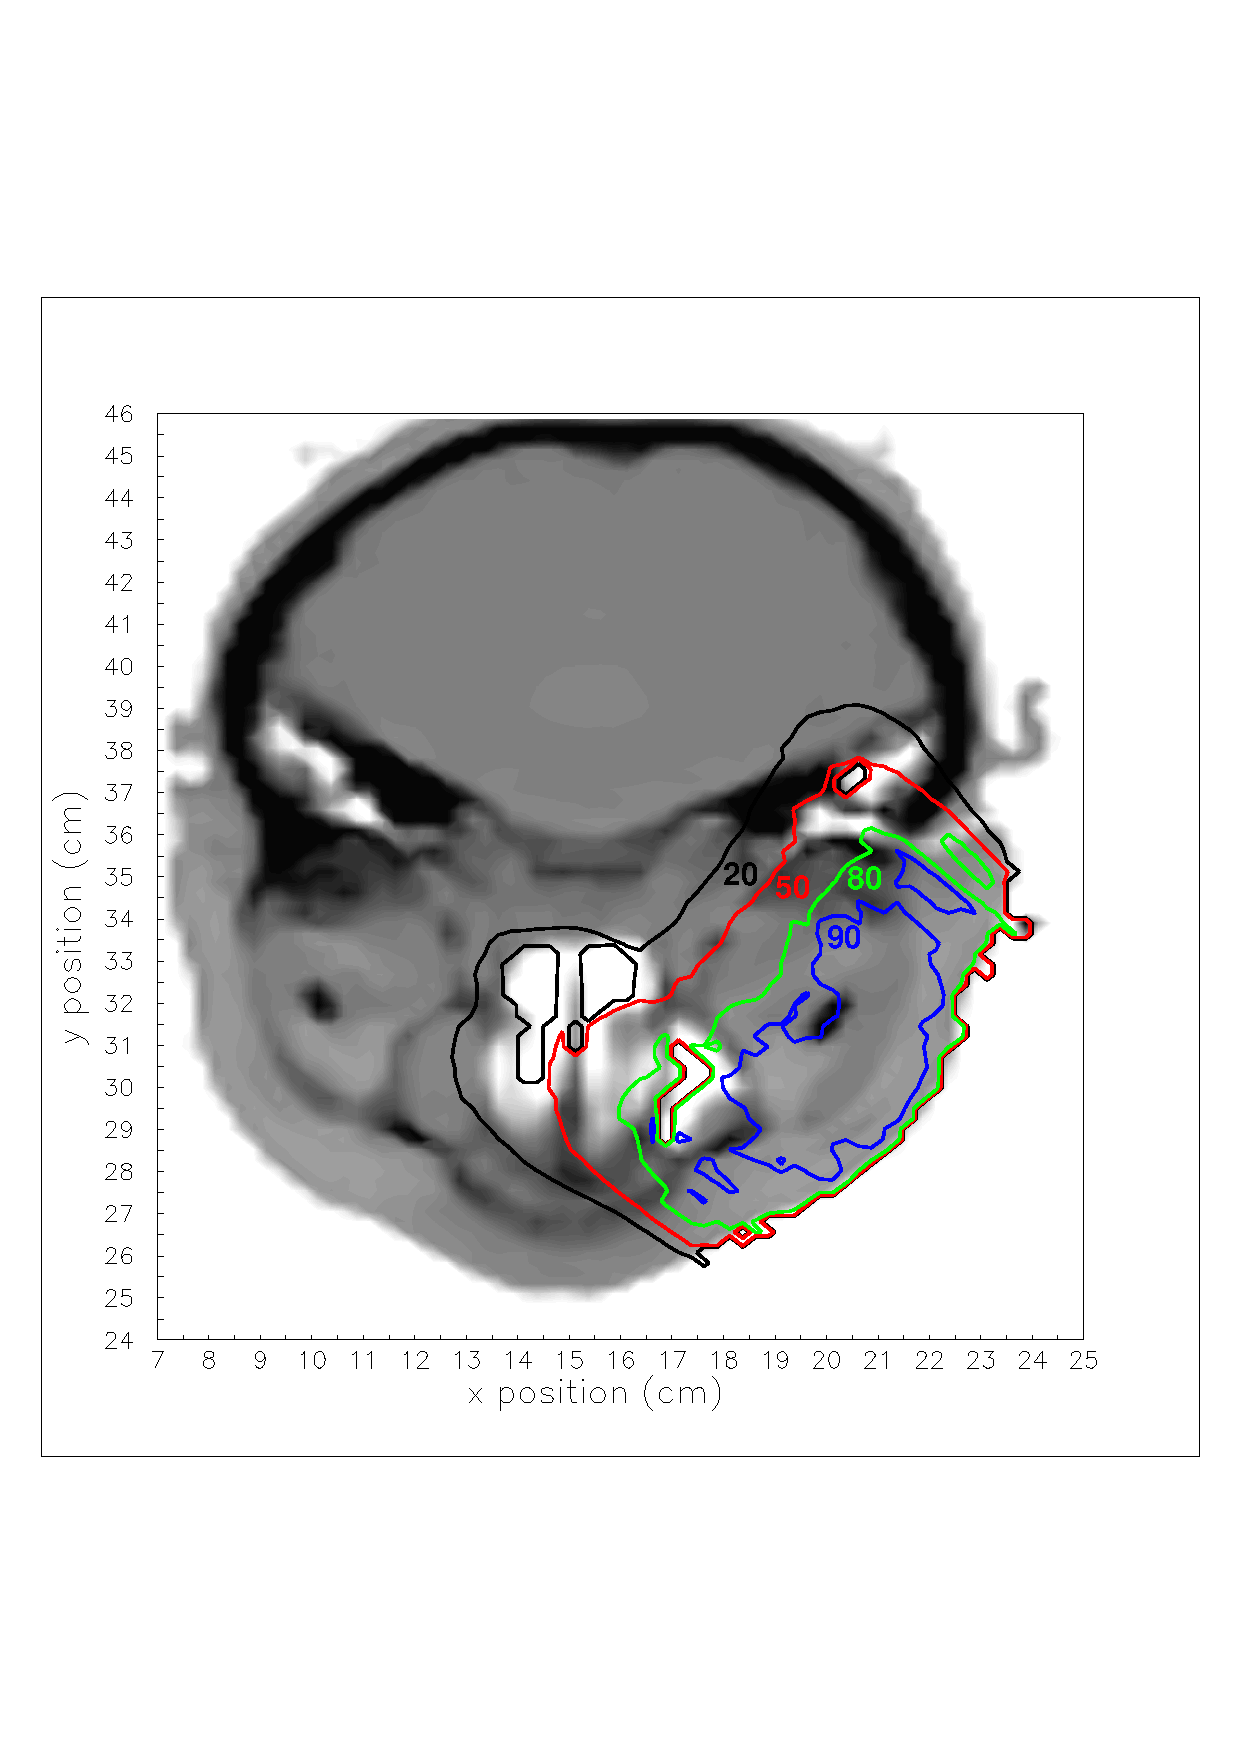
\includegraphics[height=20cm]{figures/CT_example_msmodel}
\end{center}
\end{figure}
\begin{htmlonly}       %%%%%%%%%%%%%%%%%%%%%%%%%%%%%%%%%%%%%%%%%%%%%%
\begin{rawhtml}
</center>
\end{rawhtml}
\end{htmlonly}       %%%%%%%%%%%%%%%%%%%%%%%%%%%%%%%%%%%%%%%%%%%%%%


\vfill
\copyright NRC Canada, 2021
\end{center}

\newpage
\pagestyle{fancy}
\pagenumbering{arabic}
\setcounter{page}{2}

\newpage

\setlength{\parindent}{0em}

\begin{center}
\begin{Large}
{\bf Abstract}
\end{Large}
\end{center}
\indexm{abstract}
DOSXYZnrc is an EGSnrc-based Monte Carlo simulation code for calculating
dose distributions in a rectilinear voxel phantom and is based directly
on the DOSXYZ code developed for the EGS4 code system (see NRC Report
PIRS-509B). DOSXYZnrc is part of the OMEGA-BEAM system of codes developed
at NRC.  Density and material in every voxel may vary.  A variety of beams
may be incident on the phantom, including full phase-space files from
BEAMnrc  and beams characterized using Beam Characterization models. The
companion program {\tt ctcreate} is capable of reading in a CT data set
of Hounsfield numbers and converting it into the information needed by
DOSXYZnrc to simulate transport in a phantom (i.e.  ~the appropriate
material and density are specified in each voxel).  Any of the available
beams can be incident on this CT phantom.  The code includes a restart
facility and can be run on parallel computing platforms.  The statistical
analysis is based on a history by history method as opposed to the batch
method used in DOSXYZ.

This user's manual covers general DOSXYZnrc inputs, geometries and outputs.  It
contains information on how to compile and run DOSXYZnrc using the EGSnrcMP
system. It also describes
the use of {\tt ctcreate}.

\begin{latexonly}
\vspace{11.5cm}
\end{latexonly}

\rule{16.3cm}{0.6mm}\\
\begin{small}
The figure on the front page shows a PAW visualisation of the isodose
curves from a DOSXYZ simulation in which a Clinac 2100c 18MeV electron
beam (simulated using a multiple-source model--with 35 million initial
histories) was
incident on the head and neck of a CT phantom.  The visualisation was
implemented by Daryoush Sheikh-Bagheri.

\end{small}

\newpage

\indexm{contents}
\tableofcontents

\newpage

%\pagestyle{myheadings}

\section{Introduction}

\subsection{Overview}
DOSXYZnrc is a general-purpose Monte Carlo EGSnrc\cite{Ka99a,KR00}
\indexm{EGSnrc}
user-code for 3-dimensional absorbed dose calculations. EGSnrc/DOSXYZnrc
simulates the transport of photons and electrons in a Cartesian volume and
scores the energy deposition in the designated voxels. DOSXYZnrc is ``stand
alone'', in the usual EGSnrc sense in that it is controlled by
the {\tt \*.pegs4dat} and {\tt \*.egsinp} files and
is capable of writing out ASCII formatted dose distribution arrays.  The
code uses the EGSnrcMP system which is described in detail in its own
Users Manual\cite{Ka03}.
There is also a graphical user interface (GUI) which allows
input files to be created and executed graphically\cite{TR99}.  Much of the information
in this manual is conveniently accessible via the GUI's help files.


The geometry is a rectilinear volume with
\indexm{geometry coordinate system}
the X-Y plane on the page,  X to the right, Y down the page
and the Z-axis into the page.
Voxel dimensions are completely variable in all three directions. Every
voxel (volume element) can have different materials and/or varying
densities (for use with CT data).  The code allows sources such as a
monoenergetic diverging or parallel beam, phase-space data generated by a
BEAMnrc simulation, or a model-based beam reconstruction produced by BEAMDP.
\indexm{BEAMDP}

DOSXYZnrc has a number of important and unique features such as dose
component calculations, a wide variety of source configurations and beam
reconstruction techniques, CT to phantom conversion
(via {\tt ctcreate}), restart capabilities, phase-space redistribution, \etc.
\indexm{ctcreate}

{\tt ctcreate} is a stand alone program which converts CT data sets into the
data needed for DOSXYZnrc to do a simulation. At present it handles ADAC
Pinnacle, AAPM, CADPLAN and DICOM formats for the CT files.
\indexm{Pinnacle CT}
If you develop extensions, why not
\indexm{CADPLAN CT}
\indexm{DICOM CT}
share them with your colleagues?  Send them to us and we will integrate
them into the standard distribution with full acknowledgement of the
source.

The DOSXYZnrc code, in common with the BEAMnrc system is written for a
preprocessor of Fortran77 called {\tt MORTRAN}. The user does not need
to know {\tt MORTRAN} to use the code, but its elements are needed for
modifications (see refs~\cite{Ne85} or \cite{KR00}).

\subsection{History of DOSXYZnrc}

\indexm{history of DOSXYZnrc}

DOSXYZ started out as a demonstration code that Dave Rogers wrote in March
1986 to show Ralph Nelson that special purpose coding of rectilinear
voxels was faster than using Ralph's more general macros.  At about that time
it was used to estimate the time required to do a full Monte Carlo
treatment planning calculation and the results published 3 years later in
a book chapter\cite{RB90}.  It then became the basis for a Monte Carlo
timing benchmark\cite{BR92} which was regularly updated and available
on the WWW for many years (until 2000).
The OMEGA project took this code over and
added a variety of different source routines with coding contributions
from Charlie Ma, Bruce Faddegon, George Ding, Dave Rogers,  Alex Bielajew,
and Paul Reckwerdt.  More recent modifications have reduced the array
space used by the code, and added beam characterization inputs (Charlie
Ma), btree inputs, (Brian Geiser, but no longer supported), correlated
sampling (Mark Holmes, but no longer supported).
Blake Walters and Mark Holmes added the CT
reading ability in summer 1996.  Blake Walters separated out the
{\tt ctcreate} code in summer 1997 to make the DOSXYZ code much smaller and
thus
able to handle much larger array sizes.  Blake Walters added the
{\tt dsurround} option for reducing simulation time for depth-dose curves
and dose profiles and also the coding for parallel processing in 1998.
\indexm{ctcreate} In 1999, an option was added to allow the user to
run N parallel jobs using a phase space source that exists in N
separate pieces (option now only available using the old
{\tt pprocess} script and not with the new built-in parallel processing
functionality).

Prior to the 1999 revD of this manual, the authors included Paul
Reckwerdt, Mark Holmes and Brian Geiser who had been involved with the
original code to read Pinnacle CT data sets, correlated sampling and
BTREE beam modelling respectively.  These extensions are either no longer
used or are not supported and, thus, these authors are no longer included
as authors of the users manual.  Manuals and/or notes by Geiser and Holmes
are available separately describing BTREE\cite{Ge95} and
correlated sampling\cite{Ho99}.  This latter manual used to be part of
the DOSXYZ Users Manual prior to 1999.

In 2001, with the help of Iwan Kawrakow, Blake Walters ported the
DOSXYZ code to the EGSnrc system to give DOSXYZnrc. At the same time
the statistical analysis routines were converted to a much improved,
history by history approach\cite{Wa02a} instead of the standard batch
approach used in DOSXYZ.

In 2004, Iwan Kawrakow and Blake Walters ported DOSXYZnrc to the new
EGSnrcMP system\cite{Ka03}.  This eliminated the exclusive use of Linux/Unix scripts
and allowed DOSXYZnrc to be compiled and run on Windows-based systems in
addition to Linux/Unix platforms.  At this time, DOSXYZnrc operates
similarly to a standard EGSnrcMP user code, although it is only distributed
as part of the OMEGA/BEAM system.

Although Charlie Ma is no longer an author of the DOSXYZnrc version of the
code, his major contributions to the original EGS4 version still remain.

\vfill

\subsection{Compatibility of DOSXYZ and DOSXYZnrc}

After renaming a DOSXYZ input file from {\tt filename.egs4inp} to {\tt
filename.egsinp}, the file can be used directly by DOSXYZnrc.  This is
because DOSXYZnrc assumes particular default values for all of the
additional EGSnrc input parameters needed.  However, a better approach is
to use the GUI for DOSXYZnrc ({\tt dosxyznrc\_gui}) to read in the DOSXYZ file
and then output the DOSXYZnrc input file with all of the defaults
explicitly stated.  For further information, see
section~\ref{egsnrc_inputs} on page~\pageref{egsnrc_inputs}.

The results of calculations with DOSXYZ and DOSXYZnrc will be very similar
for most situations.  The one systematic difference is that the
relativistic spin corrections to the multiple scattering cause the
depth-dose curves for electron beams to be about 1.5\% more penetrating in
water for a given
electron energy\cite{Wa00}.
\index{DOSXYZ!differences}
\index{DOSXYZ!input file compatibility}
\vfill
\newpage


\section{Compiling/running DOSXYZnrc}
\indexm{compiling!DOSXYZnrc}

\subsection{Files Related to DOSXYZnrc and ctcreate}
\label{filesect}

\indexm{\$HEN\_HOUSE}
As an EGSnrcMP user code, the DOSXYZnrc files are mostly contained in
the directory {\tt \$HEN\_HOUSE/user\_codes/dosxyznrc/},
while {\tt ctcreate} files are
\indexm{ctcreate}
in {\tt \$OMEGA\_HOME/progs/ctcreate/}.  For a general description of the
file structure see Chapter 1 of the BEAMnrc User's Manual \cite{Ro04a}.
\indexm{file structure}

The following describes some files related to DOSXYZnrc:

\begin{description}

\index{dosxyznrc\_gui}
\item[{\tt dosxyznrc\_gui}] This is the Tcl graphical user interface for
creatingi, modifying or executing DOSXYZnrc input files.  Files
related to this are located in
{\tt \$OMEGA\_HOME/progs/gui/dosxyznrc}.  See the GUI manual\cite{TR99}
for more details.
\indexm{graphical user interface}


\item [{\tt egsnrc\_cshrc\_additions} (or {\tt egsnrc\_bashrc\_additions})]
Located in\\ {\tt \$HEN\_HOUSE/scripts}.  If using a Linux/Unix system,
this file must be sourced
in the user's {\tt .cshrc} (or {\tt .bashrc}) file.  It defines useful
aliases for compiling/running DOSXYZnrc.
\indexm{files!egsnrc\_cshrc\_additions}
\indexm{files!egsnrc\_bashrc\_additions}
\indexm{egsnrc\_cshrc\_additions}
\indexm{egsnrc\_bashrc\_additions}

\indexm{Makefile}
\indexm{files!Makefile}
\item [{\tt Makefile}] Located in {\tt \$HEN\_HOUSE/user\_codes/dosxyznrc}.
This file is used by the GNU {\tt make} utility to handle compilation of
\indexm{config.conf}
\indexm{beamnrc.spec}
DOSXYZnrc.  Includes\\ {\tt \$HEN\_HOUSE/specs/config.conf}
(where {\tt config} is the configuration you are using) and
{\tt \$HEN\_HOUSE/specs/beamnrc.spec} files to define environment variables
\indexm{RANDOM}
\indexm{ranmar}
and compiler options.  Also, with the {\tt RANDOM} variable, it defines
the random number generator used (current default is {\tt ranmar}).  Finally,
\indexm{SOURCES}
it defines the variable {\tt SOURCES} which determines the
macros and MORTRAN sources that are
\indexm{mortjob.mortran}
concatenated together to create {\tt mortjob.mortran} (the code that is
actually MORTRAN compiled).
There are two versions of this file, called {\tt Makefile.MS} and  {\tt
Makefile.NOMS}, on the distribution. The default  {\tt Makefile} is  {\tt
Makefile.NOMS} which does not use multiple source models  (source 4, beam
characterization models).  {\tt Makefile.MS} is to be used when Multiple
Source models are to be used (read the file for instructions).
\indexm{beam characterization models}
\indexm{source routines!beam characterization}

\indexm{dosxyznrc.make}
\indexm{files!dosxyznrc.make}
\item[{\tt dosxyznrc.make}] Located in {\tt \$HEN\_HOUSE/user\_codes/dosxyznrc}.  This is an empty file that must exist for compilation using the
{\tt make} utility.

\item[{\tt dosxyznrc.mortran}]  Located in {\tt \$HEN\_HOUSE/user\_codes/dosxyznrc}.  Main {\tt MORTRAN} source code.
\indexm{files!dosxyznrc.mortran}
\indexm{dosxyznrc.mortran}

\item[{\tt srcxyznrc.mortran}]  Located in {\tt \$HEN\_HOUSE/user\_codes/dosxyznrc}.
Subroutines for source configuration inputs + energy spectrum
\indexm{files!srcxyznrc.mortran}
\indexm{srcxyznrc.mortran}

\item[{\tt srcxyznrc.macros}]  Located in {\tt \$HEN\_HOUSE/user\_codes/dosxyznrc}.
{\tt MORTRAN} macros required by {\tt srcxyznrc.mortran}
\indexm{files!srcxyz.macros}
\indexm{srcxyznrc.macros}

\indexm{files!read\_write\_pardose.c}
\indexm{read\_write\_pardose.c}
\indexm{.pardose}
\item[{\tt read\_write\_pardose.c}]  Located in {\tt \$HEN\_HOUSE/user\_codes/dosxyznrc}.  C subroutines used in DOSXYZnrc to
write and read binary {\tt .pardose} output during parallel jobs.  If you
have a C or C++ compiler, then this is compiled when the OMEGA/BEAM
\indexm{read\_write\_pardose.o}
system is installed and {\tt read\_write\_pardose.o} is put
in directory {\tt \$HEN\_HOUSE/lib/config}, where {\tt config} is the
name of your configuration.  If you do not have a C or C++ compiler, then
\indexm{parallel calculations}
this file is not compiled, and the built-in parallel functionality of
DOSXYZnrc cannot be used.

\indexm{files!dosxyznrc\_config.spec}
\indexm{dosxyznrc\_config.spec}
\item[{\tt dosxyznrc\_config.spec}]  (where {\tt config} is the
name of your configuration) Located in\\
{\tt \$HEN\_HOUSE/specs}.  This file is created during OMEGA/BEAM
installation and determines whether or not
the compiled C routines for reading/writing {\tt .pardose} files,
{\tt read\_write\_pardose.o}, are linked in at compile time or not.
If they are to be linked (i.e., you have a C or C++ compiler and
{\tt read\_write\_pardose.c} was compiled successfully), then
\indexm{PARDOSE\_OBJECTS}
the variable {\tt PARDOSE\_OBJECTS} in this file is set
to\\ {\tt \$(EGS\_LIBDIR)read\_write\_pardose.o}, where\\
{\tt \$(EGS\_LIBDIR)}={\tt \$HEN\_HOUSE/lib/config}.  If the
routines are not to be linked at compile time (i.e., you do not
have a C or C++ compiler or {\tt read\_write\_pardose.c} was not
compiled successfully), then {\tt PARDOSE\_OBJECTS} is left blank.

\item[{\tt dosxyznrc\_user\_macros.mortran}] Located in
{\tt \$HEN\_HOUSE/user\_codes/dosxyznrc}.  \\
{\tt MORTRAN} macros that
the user may change  - includes defaults for various options such as beam
models, \etc.  Note that {\tt dosxyznrc\_user\_macros} is also used
by ctcreate to define the maximum dimensions of the DOSXYZnrc phantom
output.
\indexm{files!dosxyznrc\_user\_macros.mortran}
\indexm{dosxyznrc\_user\_macros.mortran}

\item[{\tt dosxyznrc.io}]  Located in {\tt \$HEN\_HOUSE/user\_codes/dosxyznrc}.  This file assigns file names to Fortran unit numbers for output
files not opened explicitly in {\tt dosxyznrc.mortran}.  Currently, the
only files that use this are the {\tt .egslst} file (Fortran unit 1) and
the {\tt .errors} file (Fortran unit 15).
\indexm{files!dosxyznrc.io}
\indexm{dosxyznrc.io}

\indexm{files!phsp\_macros.mortran}
\indexm{phsp\_macros.mortran}
\item[{\tt phsp\_macros.mortran}] {\tt MORTRAN} macros used to read
phase space sources.  This file is always picked up from the
{\tt \$HEN\_HOUSE/utils} directory.

\indexm{files!iaea\_phsp\_macros.mortran}
\indexm{iaea\_phsp\_macros.mortran}
\item[{\tt iaea\_phsp\_macros.mortran}] {\tt MORTRAN} macros used to handle
IAEA-format phase space sources.  Located in the
{\tt \$HEN\_HOUSE/utils} directory, this file is only included if
EGSnrc was installed on a machine with a working C++ compiler and the
library of IAEA phase space handling routines
({\tt \$HEN\_HOUSE/iaea\_phsp/iaea\_phsp.a}) was compiled successfully.
Otherwise, these macros are defined as blank ({\tt \{;\}}) in
{\tt phsp\_macros.mortran} and IAEA functionality does not exist.

\item[{\tt beammodel\_macros.mortran}]    {\tt MORTRAN} macros required
by the multiple-source model for beam reconstruction (source 4), stored in
{\tt \$OMEGA\_HOME/progs/beamdp}.
\indexm{files!beammodel\_macros.mortran}
\indexm{beammodel\_macros.mortran}
\indexm{BEAMDP}

\item[{\tt beammodel\_routines.mortran}]    {\tt MORTRAN} subroutines
required by the multiple-source model for beam reconstruction (source 4),
stored in {\tt \$OMEGA\_HOME/progs/beamdp}.
\indexm{files!beammodel\_routines.mortran}
\indexm{beammodel\_routines.mortran}

\indexm{files!DOSXYZnrc\_examples}
\indexm{DOSXYZnrc\_examples}
\item[{\tt DOSXYZnrc\_examples/}] A subdirectory of
{\tt \$HEN\_HOUSE/user\_codes/dosxyznrc}.  This directory contains sample
input files for DOSXYZnrc.

\end{description}

The following is a description of some of the files related to
{\tt ctcreate}:

\begin{description}

\indexm{files!Makefile}
\indexm{Makefile}
\item[{\tt Makefile}] Located in {\tt \$OMEGA\_HOME/progs/ctcreate}.
Used by the GNU {\tt make} utility, this file
\indexm{SOURCES}
\indexm{mortjob.mortran}
directs the compilation of {\tt ctcreate}.  The {\tt SOURCES} variable defines
the macros and MORTRAN sources concatenated to create {\tt mortjob.mortran}
(which is ultimately MORTRAN compiled)

\item[{\tt ctcreate.mortran}] Located in {\tt \$OMEGA\_HOME/progs/ctcreate}.
This is the main {\tt MORTRAN} source code for
{\tt ctcreate}.
\indexm{files!ctcreate.mortran}
\indexm{ctcreate.mortran}

\indexm{files!ReadCT\_DICOM.c}
\indexm{ReadCT\_DICOM.c}
\indexm{DICOM format}
\item[{\tt ReadCT\_DICOM.c}] Located in {\tt \$OMEGA\_HOME/progs/ctcreate}.
This is a C subroutine for reading CT images in DICOM format.  It is linked
to {\tt ctcreate.mortran} at compile time.

\indexm{files!tags\_ct.h}
\indexm{tags\_ct.h}
\indexm{DICOM format}
\item[{\tt tags\_ct.h}] Located in {\tt \$OMEGA\_HOME/progs/ctcreate}.  This
is a C header file used with {\tt ReadCT\_DICOM.c}.  It defines the
hexadecimal data identifiers used in DICOM image format.

\item[{\tt lnblnk1\_function.mortran}]{\tt MORTRAN} macro to provide the
FORTRAN {\tt lnblnk} function for all configurations.  This is picked
up from {\tt \$HEN\_HOUSE/src}.
\indexm{files!lnblnk1\_function.mortran}
\indexm{lnblnk1\_function.mortran}

\end{description}

\subsection{Compiling and Running DOSXYZnrc}
\label{candrsect}

The commands for compiling and running DOSXYZnrc are
similar to those for other EGSnrcMP user codes
(see the EGSnrcMP Users Manual\cite{Ka03}).
For EGS4 users, please note that file extensions have
changed from, {\em eg,} {\tt file.egs4inp} to {\tt file.egsinp}.
\indexm{.egsinp}
\indexm{.egs4inp}
\indexm{files!.egsinp}
\indexm{files!.egs4inp}

\indexm{DOSXYZnrc!installation}
DOSXYZnrc is normally compiled on your user area as part of the
OMEGA/BEAM user set up
(see the BEAMnrc Manual \cite{Ro04a} for configuration instructions).
To compile DOSXYZnrc independently
(e.g., necessary if you have changed some parameters in \\
{\tt dosxyznrc\_user\_macros.mortran}), ensure that
{\tt Makefile}, {\tt dosxyznrc.make},\\ {\tt dosxyznrc.mortran},
{\tt dosxyznrc\_user\_macros.mortran}, {\tt srcxyznrc.mortran},\\
{\tt srcxyznrc.macros}, and {\tt dosxyznrc.io}
exist in your\\ {\tt \$EGS\_HOME/dosxyznrc} directory (they
should have been copied there automatically from
{\tt \$HEN\_HOUSE/user\_codes/dosxyznrc} during
OMEGA/BEAM configuration).
Then, from {\tt \$EGS\_HOME/dosxyznrc}, compile DOSXYZnrc by typing:
\indexm{make}
\begin{verbatim}
make [options]
\end{verbatim}
The options for {\tt make} are:
\indexm{make!options}
\begin{verbatim}
make              Compile with default optimization
make opt          turned on.  Default optimization is level 2 (-O2).

make noopt        Compile with no optimization

make debug        Compile executable for debugging.

make fortran      Do mortran compilation only, leaving behind the Fortran
                  file dosxyznrc.F.

make clean        Remove the Fortran file, mortjob.mortran file,
                  dosxyznrc.mortlst file and the executable.
\end{verbatim}

\indexm{mf}
\indexm{egsnrc\_cshrc\_additions}
\indexm{egsnrc\_bashrc\_additions}
\indexm{compile\_user\_code}
To preserve compatibility with old usage, the {\tt mf} command is also
available for compiling DOSXYZnrc on a Linux/Unix system (you must have
sourced\\
{\tt \$HEN\_HOUSE/scripts/egsnrc\_cshrc\_additions} or\\
{\tt \$HEN\_HOUSE/scripts/egsnrc\_bashrc\_additions} from your
{\tt .cshrc} or {\tt .bashrc} file).  {\tt mf} is
aliased to the script {\tt \$HEN\_HOUSE/scripts/compile\_user\_code}.

To use {\tt mf}, go into {\tt \$EGS\_HOME/dosxyznrc} and type:
\begin{verbatim}
m[f] dosxyznrc [a] [opt|noopt|debug]
\end{verbatim}
\index{mf!options}
The options for {\tt mf} are:
\verb+mf         =>+ Mortran and Fortran compile and then link\\
\verb+m          =>+ Mortran compile and create the Fortran file\\
\verb+opt        =>+ use optimization (default level 2)\\
\verb+noopt      =>+ use no optimization\\
\verb+debug      =>+ create executable ready for a debug run\\
The parameter ``{\tt a}" is not used and is only present for compatibility
with the previous version of {\tt mf}.

Once you have successfully compiled DOSXYZnrc, the executable,
{\tt dosxyznrc*}, will be left in your {\tt \$EGS\_HOME/bin/config} directory
(where {\tt config} is the name of the configuration that you are using).

\indexm{running DOSXYZnrc}
\indexm{input file}
\indexm{pegs data file}
To run DOSXYZnrc interactively from the command line, go into
{\tt \$EGS\_HOME/dosxyznrc} and type:
\begin{verbatim}
dosxyznrc -i inputfile -p pegsdata
\end{verbatim}
where the input file is {\tt \$EGS\_HOME/dosxyznrc/inputfile.egsinp} and the
file\\
 {\tt pegsdata.pegs4dat} contains the PEGS4 data set (it can be on
{\tt \$EGS\_HOME/pegs4/data} or if not found there, on
{\tt \$HEN\_HOUSE/pegs4/data}).

\index{ex}
If you are using a Unix/Linux system, then you can also start
an interactive DOSXYZnrc run using
the {\tt ex} (aliased to {\tt \$HEN\_HOUSE/scripts/run\_user\_code})
command:
\begin{verbatim}
ex dosxyznrc inputfile pegsdata
\end{verbatim}
{\tt ex} is provided to preserve compatibility with old usage.

\indexm{parallel jobs}
\indexm{batch jobs}
\indexm{running DOSXYZnrc!in batch}
If you are using a Linux/Unix system then you can also run DOSXYZnrc
in batch mode.  Batch submission is required for parallel jobs.
Batch submission uses the {\tt exb} command, which is aliased to
the script {\tt \$HEN\_HOUSE/scripts/run\_user\_code\_batch}.  The syntax
of the {\tt exb} command is:
\begin{verbatim}
exb dosxyznrc inputfile pegsdata [short|medium|long] [batch=batch_sys] [p=N]
\end{verbatim}
\indexm{queues}
\indexm{at} \indexm{NQS} \indexm{PBS} \indexm{keg} \indexm{SGE}
The {\tt [short|medium|long]} option defines the name of the
queue that is used (default is {\tt long} as at NRC).  The {\tt batch\_sys} input
defines the network queuing system to use.  Currently,
{\tt batch\_sys} can be set to {\tt at} (the standard Unix batch
command), {\tt pbs} (to use PBS), {\tt keg} (to use Sun's SGE) or
{\tt nqs} (for NQS).  The default is {\tt at} unless otherwise specified
by setting the environment variable {\tt \$EGS\_BATCH\_SYSTEM}.  Finally,
{\tt N} is used if you are submitting parallel jobs and is set equal to
the number of jobs that you want to split the simulation into.
\indexm{running DOSXYZnrc in parallel}
\indexm{\$EGS\_BATCH\_SYSTEM}

\indexm{temporary working directory}
Once a run is started, a temporary working directory is created as
a subdirectory of\\
{\tt \$EGS\_HOME/dosxyznrc}.  This temporary working directory
has the name\\
{\tt egsrun\_pid\_inputfile\_hostname}, where where {\tt pid} is the process ID number and {\tt hostname} is the name of the
computer the job is running on.  All output files are written
to this temporary directory.  At the end of the run, the files are moved into
{\tt \$EGS\_HOME/dosxyznrc} and the temporary working directory is
deleted.  For more information on temporary working directories, see the
EGSnrcMP Users Manual\cite{Ka03}.

\indexm{.3ddose}
\indexm{files!.3ddose}
\indexm{STATDOSE}
\indexm{output files}
\indexm{.egslst}
\indexm{.pardose}
DOSXYZnrc outputs the following files: {\tt
inputfile.egslst, inputfile.egslog} (for batch runs only, where it
contains screen output), {\tt
inputfile.egsdat} (which can be used to restart the calculation) and {\tt
inputfile.3ddose} which contains a summary of the data in all regions and
can be used by STATDOSE to create {\tt xmgr/xmgrace} graphs (see ``STATDOSE
Users Manual''\cite{MC95} ).  If this is a parallel run, then the
individual jobs will output binary {\tt .pardose} files instead of
{\tt .3ddose} files.  The {\tt .pardose} are then combined automatically at
the end of the parallel run to create a {\tt .3ddose} file.  See section~\ref{parallelcalc} for more information on parallel runs.
Note that the \indexm{inputfile} {\tt
.egslst} file can become VERY long and thereby become useless so use it
carefully for getting the dose which usually can
be more effectively obtained  via the
{\tt .3ddose} output file.
\indexm{xmgrace}
\indexm{xmgr}
\indexm{files!.egslog}
\indexm{.egsinp}
\indexm{files!.egslst}
\indexm{files!.egsdat}
\indexm{.egsdat}
\indexm{.egslog}

\indexm{compiling DOSXYZnrc!from the GUI}
\indexm{running DOSXYZnrc!from the GUI}
\indexm{dosxyznrc\_gui}
The DOSXYZnrc code can also be compiled and run from the
{\tt dosxyznrc\_gui}\cite{TR99}.
To compile DOSXYZnrc, select ``Compile'' from the ``Run'' menu.  This
will open up a window which gives you the different {\tt make} options
(ie optimization vs no optimization, debug, etc).  To run the code
from the GUI, you must first load an existing input file or create a new
one (new inputs or changes to an input file must first be saved before
running).  Then select ``Run'' from the ``Run'' menu.  This will open
up a window in which you can either run DOSXYZnrc interactively
or else submit to a queue (or start a parallel run).  Batch runs will use
the PBS queueing system unless otherwise specified in the
\indexm{\$EGS\_BATCH\_SYSTEM environment\\ variable}
{\tt \$EGS\_BATCH\_SYSTEM} environment variable.  Dialog that would normally
appear on screen during an interactive run now appears in the GUI
run window.

For more information about compiling and running user codes, see the
EGSnrcMP Users Manual\cite{Ka03}.

\subsubsection{Including source 4/beam characterization}

\label{include4}
\indexm{beam characterization models}
\indexm{files!beammodel\_macros.mortran}
\indexm{beammodel\_macros.mortran}
\indexm{files!beammodel\_routines.mortran}
\indexm{beammodel\_routines.mortran}
\indexm{source routines!beam characterization} To implement beam
characterization models in DOSXYZnrc, copy\\ {\tt beammodel\_macros.mortran}
and {\tt beammodel\_routines.mortran}, to the user's {\tt dosxyznrc} area
from {\tt \$OMEGA\_HOME/progs/beamdp}. Also copy {\tt Makefile.MS}
from\\ {\tt \$HEN\_HOUSE/user\_codes/dosxyznrc/} to the user's {\tt
dosxyznrc} area
 and rename it {\tt Makefile}.
Then recompile.
\indexm{BEAMDP}


\subsection{Statistical Analysis}

The statistical analysis in the original DOSXYZ code was done using a standard
batching technique.  Starting with DOSXYZnrc the statistics on the doses are determined by grouping scored quantities
(i.e., energy deposited) on a history-by-history basis
and then determining the uncertainties.
For most sources, this simply means
grouping quantities by incident particle.  However, for phase space sources,
where more than one incident particle may be traced back to a single
primary history, quantities are grouped by primary history.  For more
information, see the published paper on history by history
statistics in DOSXYZnrc and BEAMnrc\cite{Wa02a}.
\indexm{statistics}
\indexm{uncertainties}
\indexm{batch statistics}

It is worth noting that the method used takes into account the latent
variance in any phase space file being used as a source (i.e. the
uncertainty introduced by the statistical variations in the phase space
file). Hence, one cannot reduce the uncertainty in any dose calculation
below that level by recycling the data a large number of times.  However,
one can get an artificially low statistical result which ignores this
latent variance
if the phase space source is allowed to restart the phase space file
instead of using the recycle option (whereby each particle is used multiple
times as it is read in - see section~\ref{nrcycl}, page~\pageref{nrcycl}).
Thus, in order to get accurate uncertainty estimates,
restarting the phase space file should be avoided.
\indexm{NRCYCL}
\indexm{restart phase space}


\section{DOSXYZnrc Input Parameters}
\indexm{input parameters for DOSXYZnrc}

\subsection{Descriptions in DOSXYZnrc Source Code}
\label{DOSXYZ_input}

This section describes input parameters for DOSXYZnrc. The following descriptions
can be found in the beginning of the {\tt dosxyznrc.mortran} source code.
\indexm{graphical user interface}
The graphical user interface facilitates creation of these input files
and contains a great deal of on-line help\cite{TR99}.

\begin{small}
\input{inputs/dosxyznrc.inp}
\end{small}
\clearpage
\section{Source Routines}
\subsection{Source Types in DOSXYZnrc}
\indexm{source routines!summary}
The following source types have been developed for DOSXYZnrc:
\vspace*{-5mm}
\begin{itemize}
\item Parallel rectangular beam incident from the front (isource = 0)
\item Parallel rectangular beam  incident from any direction (isource = 1)
\item Phase-space source, particles incident from any direction
(isource = 2)
\item Point source incident from the front (isource = 3)
\item Beam characterization model, particles incident from any direction
(isource = 4)
\item Uniform isotropically radiating parallelepiped within DOSXYZnrc volume\\
(isource = 6)
\item Parallel rectangular beam incident from multiple angles (isource = 7)
\item Phase-space source incident from multiple angles (isource = 8)
\item Full BEAM treatment head simulation as source (isource = 9)
\item Full BEAM treatment head simulation as source incident from multiple
angles (isource = 10)
\item Phase space source incident
from multiple angles, with multiple SSD's and isocentres--options to run source through a shared library
geometry (defined by BEAM or other MLC code) and synchronize with geometry settings in the case of
a BEAM shared library (isource = 20)
\item BEAM treatment head simulation incident from multiple angles, with multiple SSD's and isocentres--options
to synchronize with BEAM geometry settings and run source through a shared library geometry (other MLC code) (isource = 21)
\end{itemize}
For all sources, the first input record is:\\
{\tt iqin, isource, ......}\\

\clearpage

\subsection{isource = 0: Parallel Rectangular Beam Incident from Front}
\indexm{source routines!isource = 0}
\indexm{source routines!parallel front}

The uniform parallel rectangular beam is always assumed to be incident parallel
to the Z-axis from the front of the phantom. The input parameters are:

\begin{description}
\item [~~~~{\tt iqin}] Charge of the incident beam (-1: electron, 0: photon, 1: positron)
\indexm{iqin}
\item [~~~~{\tt isource}] = 0
\item [~~~~{\tt xinl,xinu}] Lower and upper x-bounds on the phantom surface
\indexm{xinl,xinu}
\item [~~~~{\tt yinl,yinu}] Lower and upper y-bounds on the phantom surface
\indexm{yinl,yinu}
\item [~~~~{\tt thetax}] Angle of the beam relative to the x-axis (degrees)
\indexm{thetax}
\item [~~~~{\tt thetay}] Angle of the beam relative to the y-axis (degrees)
\indexm{thetay}
\item [~~~~{\tt thetaz}] Angle of the beam relative to the z-axis (degrees)
\indexm{thetaz}

\end{description}

\begin{figure}[htbp]
\begin{center}
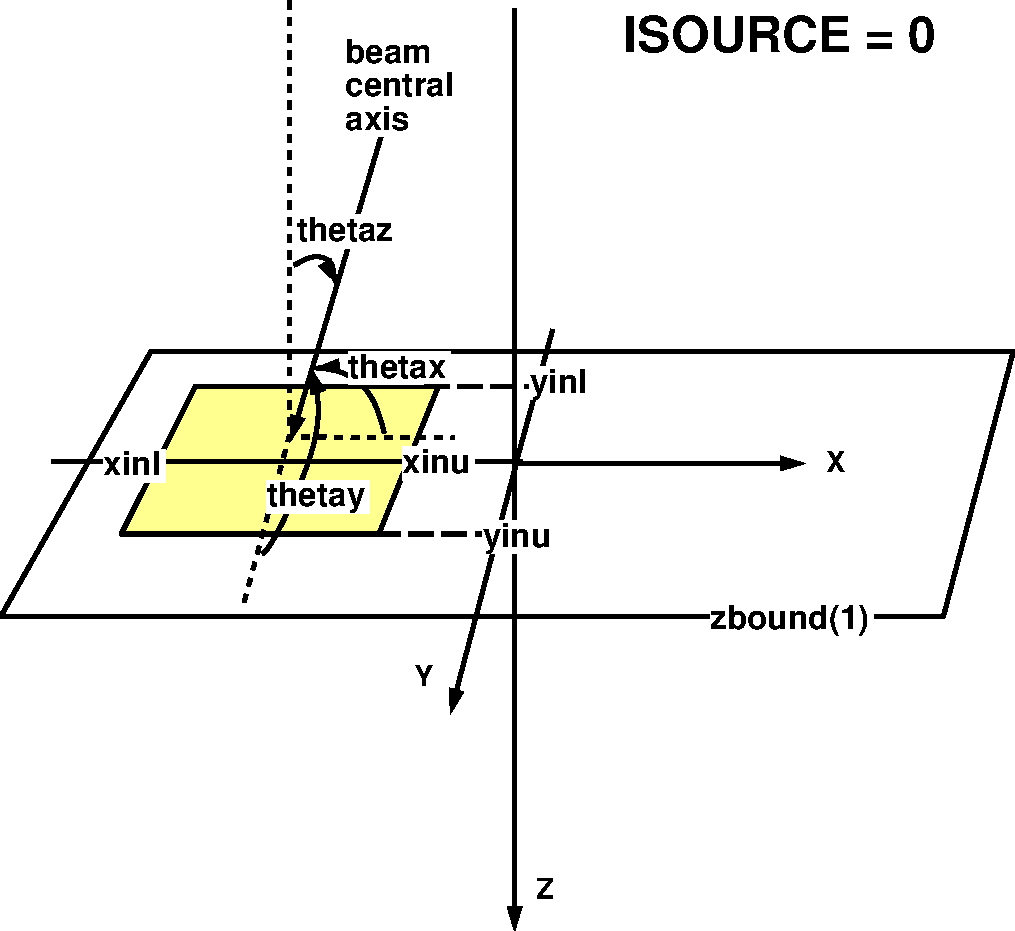
\includegraphics[height=12cm]{figures/src0}
\caption{Parallel rectangular beam (isource=0) showing the beam field, defined by
{\tt xinu}, {\tt xinl, yinu}, and {\tt yinl} on the phantom surface and the
beam directions, {\tt thetax}, {\tt thetay}, and {\tt thetaz}.
The angles {\tt thetax} and {\tt thetay} are relative to the positive x- and y-axes respectively,
while {\tt thetaz} is measured relative to the negative z-axis.}
\label{fig_src0}
\end{center}
\end{figure}
\indexm{xinl,xinu}
\indexm{yinl,yinu}
\indexm{thetax}
\indexm{thetay}
\indexm{thetaz}

\clearpage

\rfoot[]{}

\subsection{isource = 1: Parallel Rectangular Beam Incident from Any Direction}
\indexm{source routines!isource = 1}
\indexm{source routines!parallel any direction}

This uniform parallel rectangular beam may be incident from any direction. The input parameters are:

\begin{description}
\item [~~~~{\tt iqin}] Charge of the incident beam (-1: electron, 0: photon, 1: positron)
\indexm{iqin}
\item [~~~~{\tt isource}] = 1
\item [~~~~{\tt xiso/yiso/ziso}] x-, y-, z-coordinates of the isocenter.  The
isocenter is normally inside the phantom.
\indexm{xiso,yiso,ziso}

\item [~~~~{\tt theta}]   Angle between the +z direction and a line joining
the center of the beam where it strikes the phantom surface to the
isocenter.  In a polar coordinate system, this angle is known as the polar
angle and normally has a range 0-180 degrees.  Note that a centred beam
incident along the +z-axis (ie from the top) has {\tt theta}=180 degrees.
{\tt theta} is
not to be confused with {\tt thetaz} for isource=0, for which case {\tt
thetaz}=0 degrees to aim the source=0 beam along the +z-axis.
\indexm{thetaz}
\indexm{theta}


\item [~~~~{\tt phi}]      Angle  between the +x direction and the
projection on the x-y plane of the line joining the center of the beam on
the phantom surface to the isocenter on the xy plane.  In a polar
coordinate system, this angle is known as the azimuthal angle and normally
has a range 0-360 degrees.
\indexm{phi}

\item [{\tt xcol}/{\tt ycol}]  Total x- and y-widths of the beam on
the plane perpendicular to the beam direction, defined by the center of
the beam and the isocenter
\indexm{ycol}
\indexm{xcol}

\item [{\tt phicol}]  Angle by which the collimator is rotated in the
collimator plane perpendicular to the beam direction.  {\tt phicol} is
determined for {\tt theta}={\tt phi}=0.  The positive sense of rotation is
counterclockwise as one sights down the beam direction.  Note that the
effect of setting {\tt phicol}=90 degrees is the same as switching the
values of {\tt xcol} and {\tt ycol} when {\tt theta} and {\tt phi} are 0
or are both multiples of 90 degrees.
\indexm{theta}
\indexm{phicol}
\end{description}

\clearpage

\rfoot[{\sffamily \rightmark}]{{\sffamily \leftmark}}

\begin{figure}[htbp]
\begin{center}
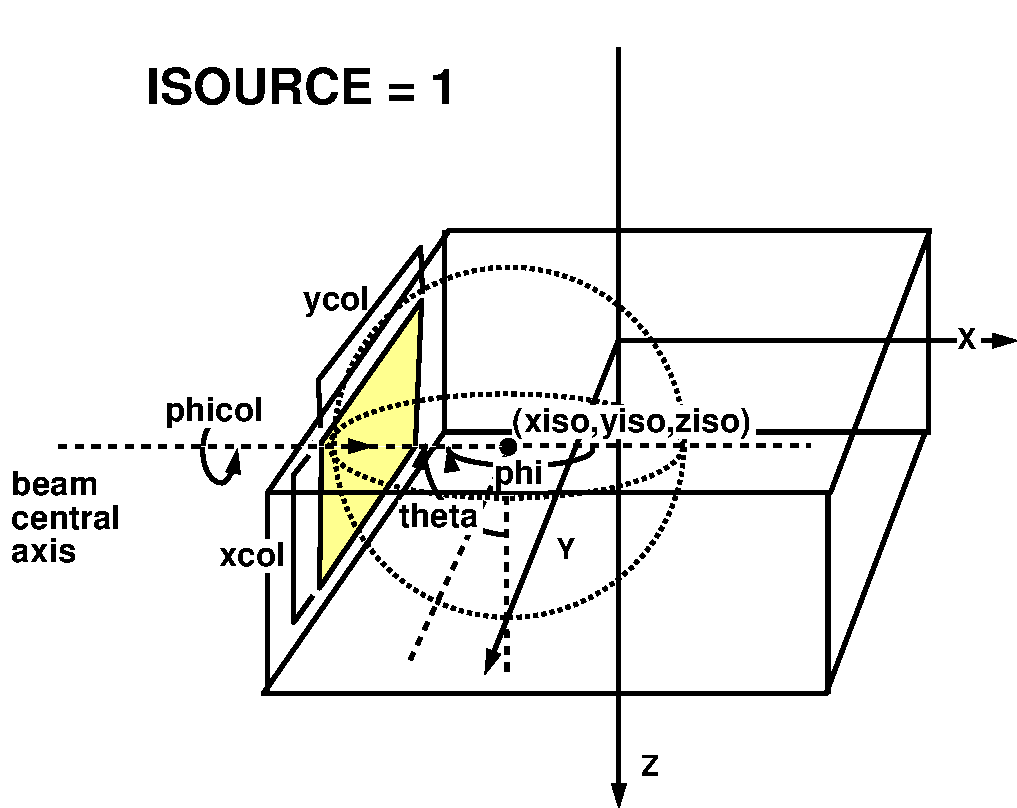
\includegraphics[width=16cm]{figures/src1}
\caption{Parallel rectangular beam incident from any direction (isource=1).  A
polar coordinate system is set up at the isocenter, (xiso,yiso,ziso).  The
position of the beam collimator is then defined using the angles, {\tt
theta} and {\tt phi}.  In the particular example shown in this figure,
with the beam incident on the centre of the negative Y face of the volume,
{\tt theta} is 90 degrees and {\tt phi} is 180 degrees.  The dimensions of
the rectangular collimator are given by {\tt xcol} and {\tt ycol}.  An
additional degree of freedom is available by allowing the collimator to
rotate in its own plane by angle {\tt phicol}.  Note that source 1 is
always incident right on the phantom surface (ie particles do not travel
through air to get to the phantom)}
\label{fig_src1}
\end{center}
\end{figure}
\indexm{xiso,yiso,ziso}
\indexm{theta}
\indexm{phi}
\indexm{phicol}

\clearpage

\subsection{isource = 2: Phase-Space Source Incident from Any Direction}
\label{source2sect}
\indexm{source routines!isource = 2}
\indexm{source routines!phase space}

This source uses a phase-space file generated during a BEAMnrc simulation at
any flat scoring plane of a linear accelerator geometry. A user can choose
any particular type of particles from the phase-space file and score dose
components using the {\tt LATCH} filter. The field size of the incident
\indexm{LATCH} beam can be reduced using the parameter {\tt BEAM\_SIZE}.
There is also a
\indexm{BEAM\_SIZE} parameter called {\tt ISMOOTH} which
can be set to 1 if one wants to shift
\indexm{ISMOOTH} the particles to
their symmetrical positions with respect to x- and y-axis in the
phase-space file for repeated use of these phase-space particles. For {\tt
ISMOOTH} = 0, no shift will be made when phase-space particles are
re-used.  {\tt LATCH} filter, {\tt BEAM\_SIZE} and {\tt ISMOOTH} are input
later in the file.
\indexm{re-use of phase space}

Input parameters for a phase-space source are:
\begin{description}
\item [~~~~{\tt iqin}] Charge of the incident beam (-1: electron, 0:
\indexm{iqin}
            photon, 1: positron, 2: all particle types)
\item [~~~~{\tt isource}] = 2
\item [~~~~{\tt xiso/yiso/ziso}] x-, y-, z-coordinates of the isocenter
\indexm{xiso,yiso,ziso}
                 (normally located within the phantom)
\item [~~~~{\tt theta}]   Same as for isource=1.
\indexm{theta}

\item [~~~~{\tt phi}]     Same as for isource=1.
\indexm{phi}
\item [~~~~{\tt dsource}]      For a BEAMnrc format phase space source, this
is the absolute distance from the isocenter to the
source center, which is, by definition, the origin of the phase-space
plane (origin may not even be in the beam).  For an IAEA format phase
space source, this is the distance from the isocentre to the primary
source ({\it i.e.} the source used to generate the phase space file), or
SAD.
\indexm{dsource}

\item [~~~~{\tt phicol}]  Angle by which the source is rotated in the
                     source plane perpendicular to the beam direction.
                     {\tt phicol} is determined for {\tt theta}={\tt phi}=0.
                     The positive sense of rotation is counterclockwise
                     as one sights down the beam direction.
\indexm{phicol}

\indexm{DBS}
\indexm{directional bremsstrahlung splitting}
\item [~~~~{\tt i\_dbs}] Set to 1 if the phase space source was generated
using directional bremsstrahlung splitting (DBS) in BEAM {\bf AND} you
wish to reject photons directed outside the splitting field (which will
all be fat).  Set to 0 otherwise.  Note that {\tt i\_dbs} is read in as
a real and converted to integer.
\indexm{i\_dbs}

\item [~~~~{\tt r\_dbs}] Radius (in cm) of the DBS splitting field in
the BEAMnrc simulation used to generate this source. Only needed if {\tt
i\_dbs} = 1.
\indexm{r\_dbs}

\item [~~~~{\tt ssd\_dbs}] SSD (in cm) where the DBS splitting field radius
was defined in the BEAMnrc simulation used to generate this source.
Only needed if {\tt i\_dbs} = 1.
\indexm{ssd\_dbs}

\item [~~~~{\tt z\_dbs}] Z value (in cm) in the BEAMnrc simulation
where this phase space source was scored.  This will be at the back of
a component module (CM).  Only needed if {\tt i\_dbs} = 1.
\indexm{{\tt z\_dbs} }

\item [~~~~{\tt e\_split}]  Number of times to split charged particles
as soon as they enter the phantom geometry.  Split particles have their
weight reduced by a factor of 1/{\tt e\_split}.  This is only used
in conjunction with photon splitting ({\tt n\_split}, see Section~\ref{nsplitsect}) and
prevents higher-weight contaminant electrons from compromising statistics
in photon beams.  For maximum efficiency, it is suggested that you
set {\tt e\_split}={\tt n\_split}, the photon splitting number.
\indexm{source 2!charged particle splitting}
\indexm{e\_split}

\indexm{{\tt FILNAM}}
\item [~~~~{\tt FILNAM}] The full name (including extension) of the phase space file
(including the directory path).  In the case of an IAEA-format phase space
source, the full name of the phase space data ({\tt .IAEAphsp}) file
\indexm{IAEA phase space source}
is input here.  The header ({\tt .IAEAheader}) file as assumed to exist
in the same directory.  For more information about IAEA-format date, see
the BEAMnrc Manual.

\end{description}

{\tt theta}, {\tt phi} and {\tt dsource} can be set to place the source
anywhere inside the phantom or the surrounding region; the medium and the
thickness of the surrounding region is input by the user.  Particles from
the phase space which are initially outside both the phantom and surrounding
region are terminated immediately.  If the medium of the surrounding
region is air, for example,  the phase-space particles will be transported
{\it properly} through air to the surface of the phantom. A particle
history is terminated if it is determined that the particle will not make
it to the phantom surface (the particle loses all its energy in the
surrounding region or it escapes through the outer boundaries of the
surrounding region).


Note that, for source 2, the user must set {\tt enflag} = 2 or 3, input
the \indexm{enflag}
mode of the phase-space file (0 or 2), and input the medium number and the
thickness for the surrounding region.  The user should also input the
phase-space file name after the above inputs.  These other inputs are
described in sections 5 and 6 below.  For more information related to
phase-space sources, see the section on phase-space files in the
BEAMnrc User's Manual
\cite{Ro04a}.

The value of {\tt phicol} must be set to 180 degrees in order for the X-Y
coordinates in a BEAMnrc-generated phase space source to map onto the
equivalent X-Y coordinates in DOSXYZnrc.  This is because of the general
coordinate transformation done going from BEAMnrc to DOSXYZnrc.

\subsubsection[DBS Inputs]{Inputs related to directional bremsstrahlung
splitting}
\label{i_dbs_sect}

\indexm{DBS}
\indexm{directional bremsstrahlung splitting}
\indexm{fat photons}
If you have used the directional bremsstrahlung splitting (DBS) variance
reduction technique (see the BEAMnrc User's Manual\cite{Ro04a} for more
details) to
generate the phase space source, then it is recommended that you use
the inputs {\tt i\_dbs}, {\tt r\_dbs}, {\tt ssd\_dbs} and {\tt z\_dbs} to
prevent unsplit, high-weight (``fat") photons which are outside the
splitting field from compromising your dose statistics.
{\tt r\_dbs} and {\tt ssd\_dbs} (the DBS splitting field radius and
SSD in cm) are available directly from the inputs for DBS in the BEAM
simulation, while {\tt z\_dbs} is simply the Z value at the back of the
component module (CM) in the BEAMnrc simulation in which this phase space source was scored.  If
{\tt i\_dbs} is set to 1, then before a photon is used in the DOSXYZnrc
simulation, it is projected along its trajectory from {\tt z\_dbs}
to {\tt ssd\_dbs} (we assume {\tt ssd\_dbs}$\geq${\tt z\_dbs}).  If it
falls outside {\tt r\_dbs} at {\tt ssd\_dbs}, then the photon is
not used in the DOSXYZnrc simulation.  In the context of the BEAM simulation
this photon will not have been split and will be fat (but this information
is not carried in the phase space file except indirectly because of the
larger weight which is not a unique specifier).  To be able to ignore these
fat photons and thereby increase the efficiency considerably, it is
important to ensure that the dose from the photons being ignored is
negligible. This can usually be arranged by making the splitting field big
enough.
\indexm{DBS}
\indexm{directional bremsstrahlung splitting}

Note that charged particles are not
rejected with this technique, which means that if you do not want fat charged
particles to compromise dose statistics (especially near the surface of a
phantom) then you must use the electron splitting option in DBS
(again, see the BEAMnrc User's Manual for more details).

\subsubsection{IAEA format phase space sources}
\label{src2iaeasect}
\indexm{source 2!IAEA format phase space file}
In the case of an IAEA format phase space source, the input, {\tt dsource} (see above), defines the distance
from the primary source ({\it i.e.} the source used to generate the phase space file) to the phantom
isocentre, or SAD.  This is because, unlike BEAMnrc format phase space files, the incident Z-position of
particles is available and read from either the phase space data (in the case of 3-D phase space files) or the header file
(in the case of planar phase space files, such as those scored by BEAMnrc).  The input value of {\tt dsource} is then
subtracted from this Z-position to give the distance along the beam axis from the phantom isocentre to the
particle incident position.

The ability of source 2 to automatically handle IAEA phase space files in which the Z-position for each
particle is scored (3-D data) is particularly useful in cases where the phase space data available for
an accelerator is scored on a non-planar surface (as is the case with the data that Varian has made
available for their TrueBeam accelerators) or when using 3-D phase space data scored by an upstream
DOSXYZnrc simulation (see Section~\ref{phspoutsect}).

\begin{figure}[htbp]
\begin{center}
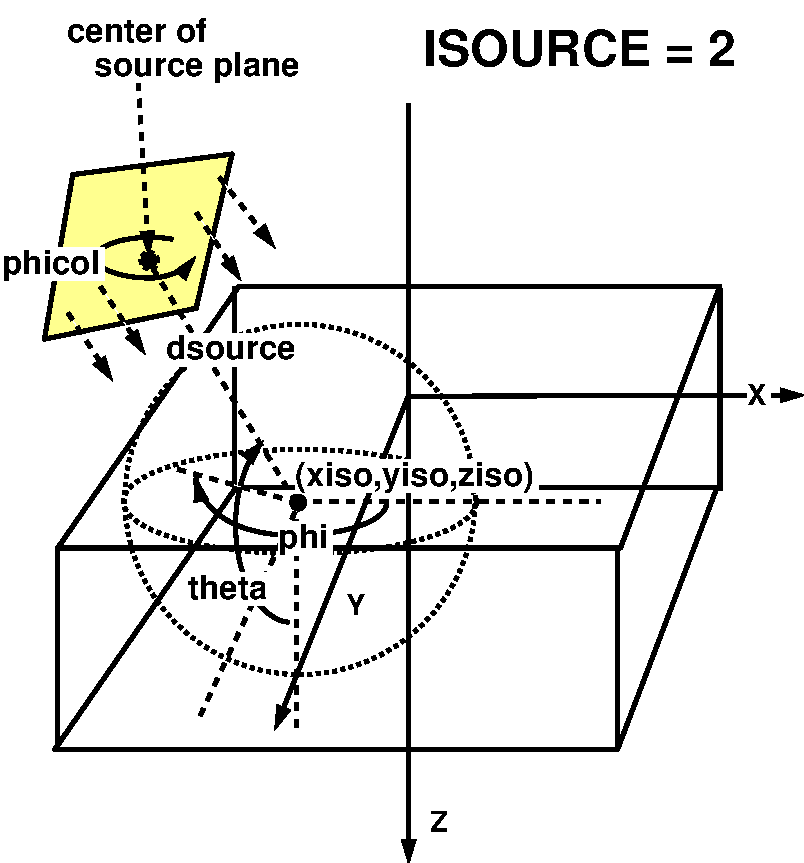
\includegraphics[width=14cm]{figures/src2}
\caption{Phase-space source incident from any direction (isource=2).
Similar to
source 1, a polar coordinate system is set up at the isocenter, (xiso,
yiso, ziso).  The position of the origin in the phase-space plane is then
defined by the angles {\tt theta} and {\tt phi}, and the distance from the
isocenter, {\tt dsource}.  The source can be rotated in its own plane
using the variable {\tt phicol}.  The figure shows that the source plane
does not necessarily have to be right against the surface of the phantom,
however it must be within the surrounding region specified by {\tt dsurround}
 (see section ~\ref{sec5}).}
\label{fig_src2}
\end{center}
\end{figure}
\indexm{dsource}
\indexm{phicol}
\indexm{theta}
\indexm{phi}
\indexm{xiso,yiso,ziso}
\indexm{dsurround}

\clearpage

\subsection{isource = 3: Point Source Rectangular Beam Incident from Front}
\indexm{source routines!isource = 3}
\indexm{source routines!point source rectangle}

The isotropically-radiating point source is placed on the Z-axis.  It is
assumed to be incident on the front surface of the phantom, but can be
placed any distance above the phantom.  The beam field can be asymmetric.

The input parameters for the point source are:
\begin{description}

\item [~~~~{\tt iqin}] Charge of the incident beam (-1: electron, 0:
\indexm{iqin}
                  photon, 1: positron)
\item [~~~~{\tt isource}] = 3
\item [~~~~{\tt xinl,xinu}] Lower and upper x-bounds of the field on the
\indexm{xinl,xinu}
          phantom surface
\item [~~~~{\tt yinl,yinu}] Lower and upper y-bounds of the field on the
\indexm{yinl,yinu}
                   phantom surface
\item [~~~~{\tt ssd}] Distance from the point source to the phantom surface (cm)
\indexm{ssd}
\end{description}

Note that, between the source and the phantom surface the medium is
assumed to be a vacuum for this source.

\begin{figure}[htbp]
\begin{center}
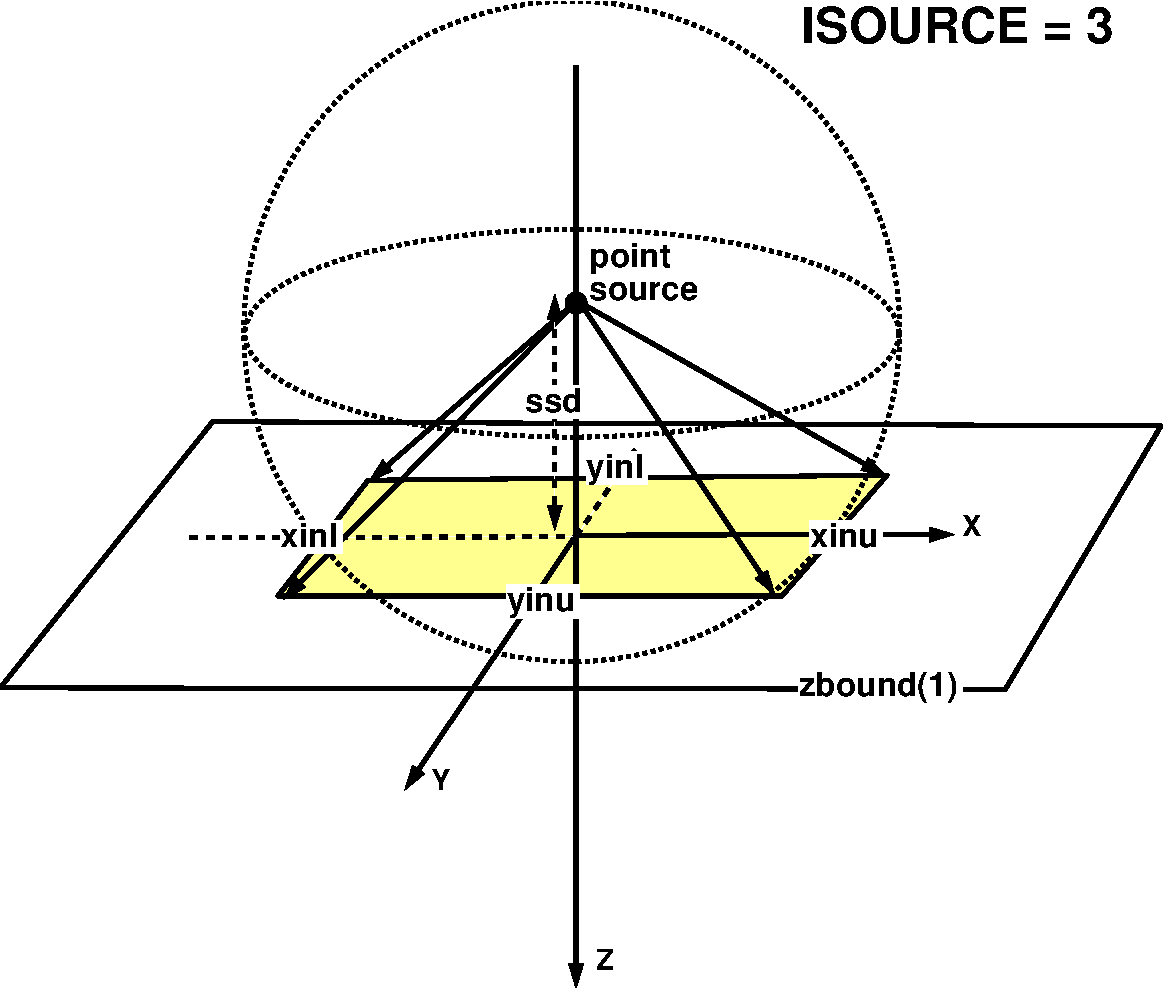
\includegraphics[height=11cm]{figures/src3}
\caption{Point source incident from the front (isource=3).  The
isotropically-radiating point source is located on the Z-axis at distance
ssd above the phantom.  The source is collimated to a rectangular field
defined by xinu, xinl, yinu, yinl on the phantom surface.}
\label{fig_src3}
\end{center}
\end{figure}
\indexm{xinl,xinu}
\indexm{yinl,yinu}

\clearpage


\subsection{isource = 4: Beam Characterization Model Incident
from Any Direction}
\indexm{source routines!isource = 4}
\indexm{source routines!beam characterization}

This source uses the beam characterization models created by BEAMDP from
phase space
data generated by BEAMnrc. This source consists of a variety of sub-sources
for different types of particles coming from different components of a
linear accelerator. Each sub-source has its own spectral and (planar)
fluence distributions and the correlation between the energy, position and
incident angle is retained by sampling the particle positions on the
sub-source (the surface of the component) and on the phase-place plane. A
beam model input file, generated by BEAMDP, is required by this source.
For more details about beam characterization models see the
BEAMnrc User's Manual and associated paper\cite{Ma95c,Ma97}.
\indexm{BEAMDP}

Apart from {\tt isource}, which must be set to 4, input parameters for source 4 are the same as for source 2:

\indexm{enflag}
Note this source requires {\tt enflag} = 4 and to input the beam model
input file name after the {\tt enflag} input. The field size of the
incident beam can be reduced using the parameter {\tt BEAM\_SIZE}.  These
inputs are described in sections 5 and 6 below.
\indexm{BEAM\_SIZE}

The default version of DOSXYZnrc does not include this source. In order to
use it you must recompile DOSXYZnrc using the instructions in
section~\ref{include4}. .

\clearpage

\rfoot[]{}

\subsection{isource = 6: Uniform Isotropically Radiating Parallelepiped
within DOSXYZnrc Volume}
\indexm{source routines!isource = 6}
\indexm{source routines!beam characterization}

This source allows the user to simulate a uniform isotropically radiating
rectangular volume (parallelepiped) within the DOSXYZnrc phantom.
The active volume is restricted to being completely contained within the
DOSXYZnrc phantom.  However, it can be shrunk to a point anywhere within the
phantom.

The input parameters for the uniform isotropically radiating parallelepiped:
\begin{description}

\item [~~~~{\tt iqin}] Charge of the incident beam (-1: electron, 0:
\indexm{iqin}
                  photon, 1: positron)
\item [~~~~{\tt isource}] = 6
\item [~~~~{\tt xinl,xinu}] Lower and upper x-bounds of the active volume (cm)
\indexm{xinl,xinu}
\item [~~~~{\tt yinl,yinu}] Lower and upper y-bounds of the active volume (cm)
\indexm{yinl,yinu}
\item [~~~~{\tt zinl,zinu}] Lower and upper z-bounds of the active volume (cm)
\indexm{zinl,zinu}
\end{description}

\begin{figure}[htbp]
\begin{center}
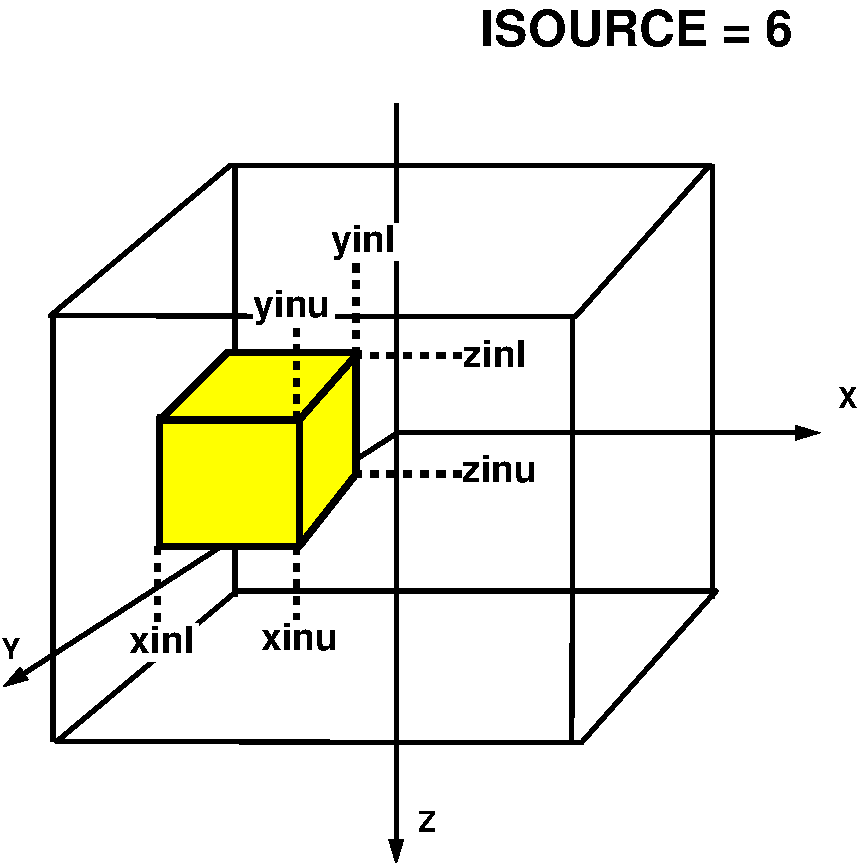
\includegraphics[height=11cm]{figures/src6}
\caption{Uniform isotropically radiating parallelepiped within DOSXYZnrc phantom
(isource=6).  The active volume, specified by {\tt xinl, xinu, yinl,
yinu, zinl, zinu}, must fit within the phantom.  The source can be shrunk
to a point within the phantom by setting {\tt xinu=xinl}, {\tt yinl=yinu}
and {\tt zinl=zinu}.}
\label{fig_src6}
\end{center}
\end{figure}
\indexm{xinl,xinu}
\indexm{yinl,yinu}
\indexm{zinl,zinu}

\clearpage

\subsection{isource = 7: Parallel Rectangular Beam Incident from Multiple Directions}
\label{source7_sec}
\indexm{source routines!isource = 7}
\indexm{source routines!parallel multiple directions}

This is a uniform parallel rectangular beam similar to source 1,
but incident from multiple, user-defined
directions (theta-phi pairs). The input parameters are:

\begin{description}
\item [~~~~{\tt iqin}] Charge of the incident beam (-1: electron, 0: photon, 1: positron)
\indexm{iqin}
\item [~~~~{\tt isource}] = 7
\item [~~~~{\tt xiso/yiso/ziso}] x-, y-, z-coordinates of the isocenter.  The
isocenter is normally inside the phantom.
\indexm{xiso,yiso,ziso}

\item [~~~~{\tt nang}]  The number of incident theta-phi pairs
or, if negative, then abs({\tt nang}) is the number of groups of
incident theta-phi pairs, where, within a group, all theta-phi pairs have
equal probability.  The incident angles theta and phi are defined the
same as they are in source 1.  Theta-phi pairs/groups are specified on
separate lines (see below).
\indexm{nang}
\indexm{theta-phi pairs}

\item [~~~~{\tt xcol}/{\tt ycol}]  Total x- and y-widths of the beam on
the plane perpendicular to the beam direction, defined by the center of
the beam and the isocenter
\indexm{ycol}
\indexm{xcol}

\item [~~~~{\tt phicol}]  Angle by which the collimator is rotated in the
collimator plane perpendicular to the beam direction.  {\tt phicol} is
defined the same way as in source 1.
\indexm{phicol}
\end{description}

And then, on the subsequent {\tt abs(nang)}  lines:\\

{\bf If {\tt nang} $>$ 0:}\\
~~~\\
For i=1,{\tt nang}: {\tt theta(i), phi(i), pang(i)}
\begin{description}
\item [~~~~{\tt theta(i)}]  Theta for pair i (degrees).
\item [~~~~{\tt phi(i)}]  Phi for pair i (degrees).
\item [~~~~{\tt pang(i)}] Probability of particle being incident at
                          Theta(i)-Phi(i).
\indexm{theta(i)}
\indexm{phi(i)}
\indexm{pang(i)}
\end{description}
{\bf If {\tt nang} $<$ 0:}\\
~~~\\
For i=1,-{\tt nang}: {\tt ivary(i), angfixed(i), angmin(i), angmax(i),
ngang(i), pgang(i)}
\begin{description}
\item [~~~~{\tt ivary(i)}] Set to 0 to vary phi in group i; Set to 1 to vary
theta in group i.
\item [~~~~{\tt angfixed(i)}] Fixed theta ({\tt ivary(i)}=0) or phi
({\tt ivary(i)}=1) in group i (degrees).
\item [~~~~{\tt angmin(i)}] Minimum varying phi ({\tt ivary(i)}=0) or
theta ({\tt ivary(i)}=1) in group i (degrees).
\item [~~~~{\tt angmax(i)}] Maximum varying phi ({\tt ivary(i)}=0) or
theta ({\tt ivary(i)}=1) in group i (degrees).
\item [~~~~{\tt ngang(i)}] Number of equally-spaced phi ({\tt ivary(i)}=0) or
theta ({\tt ivary(i)}=1) between and including {\tt angmin(i)} and
{\tt angmax(i)} in group i (Note that, since it includes
{\tt angmin(i)} and {\tt angmax(i)}, {\tt nang(i)} must be $\geq$ 2).
\item [~~~~{\tt pgang(i)}] Probability of particle being in group i.  Within
a group, all theta-phi pairs have equal probability.
\indexm{ivary(i)}
\indexm{angfixed(i)}
\indexm{angmin(i)}
\indexm{angmax(i)}
\indexm{ngang(i)}
\indexm{pgang(i)}
\end{description}

Note that the {\tt pang(i)} are automatically normalized.


\subsection{isource = 8: Phase-Space Source Incident from Multiple Directions}
\label{src8sect}
\indexm{source routines!isource = 8}
\indexm{source routines!phase space from multiple\\ directions}

This source is similar to source 2, except that it is incident from
multiple, user-defined directions (theta-phi pairs).

Input parameters for source 8 are:
\begin{description}
\item [~~~~{\tt iqin}] Charge of the incident beam (-1: electron, 0:
\indexm{iqin}
            photon, 1: positron, 2: all particle types)
\item [~~~~{\tt isource}] = 8
\item [~~~~{\tt xiso/yiso/ziso}] x-, y-, z-coordinates of the isocenter
\indexm{xiso,yiso,ziso}
                 (normally located within the phantom)

\item [~~~~{\tt nang}]  The number of incident theta-phi pairs
or, if negative, then abs({\tt nang}) is the number of groups of
incident theta-phi pairs, where, within a group, all theta-phi pairs have
equal probability.  The incident angles theta and phi are defined the
same as they are in source 2.  Theta-phi pairs/groups are specified the
same way as they are in source 7 (see section~\ref{source7_sec} above).
\indexm{nang}
\indexm{theta-phi pairs}

\item [~~~~{\tt dsource}]      For BEAMnrc phase space files, this
is the absolute distance from the isocenter to the
source center, which is, by definition, the origin of the phase-space
plane (origin may not even be in the beam).  For IAEA phase space files, this
is the primary source to isocentre distance (SAD).
\indexm{dsource}

\item [~~~~{\tt phicol}]  Angle by which the source is rotated in the
                     source plane perpendicular to the beam direction.
                     {\tt phicol} is determined for {\tt theta}={\tt phi}=0.
                     The positive sense of rotation is counterclockwise
                     as one sights down the beam direction.
\indexm{phicol}
\indexm{DBS}
\indexm{directional bremsstrahlung splitting}
\item [~~~~{\tt i\_dbs}] Set to 1 if the phase space source was generated
                     using directional bremsstrahlung splitting (DBS) in
                     BEAMnrc {\bf AND} you wish to reject photons directed outside
                     the splitting field (which will all be fat).  Set to 0 otherwise.
		Note that {\tt i\_dbs} is read in as a real and converted to integer.
\indexm{i\_dbs}
\item [~~~~{\tt r\_dbs}] Radius (in cm) of the DBS splitting field in
the BEAMnrc simulation used to generate this source. Only needed if {\tt
i\_dbs} = 1.  \indexm{r\_dbs}

\item [~~~~{\tt ssd\_dbs}] SSD (in cm) where the DBS splitting field
radius was defined in the BEAMnrc simulation used to generate this
source. Only needed if {\tt i\_dbs} = 1.  \indexm{ssd\_dbs}

\item [~~~~{\tt z\_dbs}] Z value (in cm) in the BEAMnrc simulation
where this phase space source was scored.  This will be at the back of
a component module (CM). Only needed if {\tt i\_dbs} = 1.  \indexm{{\tt
z\_dbs} }

\indexm{e\_split}
\indexm{source 8!charged particle splitting}
\item [~~~~{\tt e\_split}] Number of times to split charged particles
as soon as they enter the phantom.  The weight of split particles
is reduced by a factor of 1/{\tt e\_split}.  This is used in
conjunction with photon splitting (input variable {\tt n\_split}, see
Section~\ref{nsplitsect}) to prevent higher-weight contaminant electrons
from compromising dose statistics.  For optimum efficiency,
set {\tt e\_split}={\tt n\_split}.

\indexm{{\tt FILNAM}}
\item [~~~~{\tt FILNAM}] The full name (including extension) of the phase space
file
(including the directory path).  See the description of
source 2 (Section~\ref{source2sect}) for more details.
\end{description}
An example may help illustrate this input.  The following input:
\typeout{}
\typeout{*******Example end of 4.9 has two extra variables??  *************}
\typeout{*******Example end of 4.9 has two extra variables??  *************}
\typeout{*******Example end of 4.9 has two extra variables??  *************}
\typeout{}
\begin{verbatim}
0, 8, 0.0, 0.0, 0.0, -1.0, 80.0, 90.0, 0.0, 0.0, 0, 0.0, 0.0, 0.0
1, 90.0, 0.0, 356.40, 100, 1.0
\end{verbatim}
is for source 8. The phase space file rotates about the isocenter at
(0,0,0). The centre of the phase-space is 80 cm from the isocenter and the
collimator angle is 90 degrees.
The -1.0 indicates there is only one group of angles. The 1 at the start of
the second line tells us that phi is fixed (at 90 degrees)
and that theta is varying, in
this case in 100 discrete steps between 0 and 356.4 degrees with equal
intensity at each angle.  In this example, {\tt i\_dbs} is set to 0, indicating
that either directional bremsstrahlung splitting (DBS) was not used in the
BEAMnrc simulation that generated this source or else the user does not wish
to reject high-weight (``fat") photons created by DBS.

For more information on how to use the inputs {\tt i\_dbs},
{\tt r\_dbs}, {\tt ssd\_dbs} and {\tt z\_dbs} see section~\ref{source2sect}
on source 2 above.

Similar to source 2, source 8 automatically handles IAEA format phase space sources
with Z-position scored for each particle (3-D phase space).

\subsection{isource = 9: BEAM Treatment Head Simulation Incident from Any
Direction}
\label{src9sect}
\indexm{source routines!isource = 9}
\indexm{source routines!full BEAM simulation}

This source uses particles sampled from a BEAM simulation running
concurrently with the DOSXYZ
\indexm{BEAM accelerator code}
simulation.  The BEAM accelerator code must be compiled as a shared
library (existing in directory {\tt \$EGS\_HOME/bin/config}, where
{\tt config} is the name of your configuration) and must be supplied
with its own input file and pegs data file.  More details about this
are given below.  Source particles for DOSXYZ are then sampled from what
would be the scoring plane during a normal run of the BEAM accelerator.
Thus, this source is similar to {\tt isource}=2 (full phase space file)
without the need to store a phase space file.

\indexm{C/C++ compiler}
\indexm{config.conf file}
\indexm{BEAMLIB\_OBJECTS}
\indexm{BEAMLIB\_EXTRA\_LIBS}
Note that if you are running on Unix/Linux you must have a working C/C++
compiler to use this source and the file
{\tt \$HEN\_HOUSE/specs/config.conf} ({\it i.e.} file {\tt \$EGS\_CONFIG})
must have the variable
{\tt BEAMLIB\_OBJECTS} set to
\indexm{load\_beamlib.o}
{\tt \$(HEN\_HOUSE)lib/\$(my\_machine)/load\_beamlib.o} and\\
{\tt BEAMLIB\_EXTRA\_LIBS} set to {\tt $-$ldl}.
If you have installed EGSnrcMP on a Unix/Linux system with a working C/C++
compiler, the installation will automatically compile the C code
\indexm{load\_beamlib.c}
{\tt \$HEN\_HOUSE/cutils/load\_beamlib.c} to create
{\tt load\_beamlib.o}, and {\tt BEAMLIB\_OBJECTS} and
{\tt BEAMLIB\_EXTRA\_LIBS} will
automatically be set to their proper values.  Otherwise
{\tt BEAMLIB\_OBJECTS} and
{\tt BEAMLIB\_EXTRA\_LIBS} will remain
undefined (ie definitions left blank).

If you are running on Windows, then there is no requirement to have
a working C/C++ compiler to use this source.  In this case, the installation
automatically sets {\tt BEAMLIB\_OBJECTS} in
{\tt \$HEN\_HOUSE/specs/config.conf} to
\indexm{load\_beamlib.obj}
{\tt \$(HEN\_HOUSE)lib/\$(my\_machine)/load\_beamlib.obj}, where
{\tt load\_beamlib.obj} is a precompiled version of {\tt load\_beamlib.o}
included with the installation.  {\tt BEAMLIB\_EXTRA\_LIBS} does not
need to be defined and is left
blank.  See the BEAMnrc Manual\cite{Ro04a} for more information about
{\tt config.conf} files.

Similar to {\tt isource = 2}, you can select particles from the BEAM simulation
\indexm{LATCH}
to use based on their charge and/or {\tt LATCH} values.   You can also
select the size of the BEAM field considered using the
\indexm{BEAM\_SIZE}
{\tt BEAM\_SIZE} input (discussed in more detail in its own section below).

Input parameters for source 9 are:
\begin{description}
\item [~~~~{\tt iqin}] Charge of the incident beam (-1: electron, 0:
\indexm{iqin}
            photon, 1: positron, 2: all particle types)
\item [~~~~{\tt isource}] = 9
\item [~~~~{\tt xiso/yiso/ziso}] x-, y-, z-coordinates of the isocenter
\indexm{xiso,yiso,ziso}
                 (normally located within the phantom)
\item [~~~~{\tt theta}]   Same as for isource=2.  Recall that, for a
beam coming down from the top of the phantom, {\tt theta}=180 degrees.
\indexm{theta}

\item [~~~~{\tt phi}]     Same as for isource=2.
\indexm{phi}
\item [~~~~{\tt dsource}]      Absolute distance from the isocenter to the
centre of the source plane, which is, by definition, the origin of the
scoring plane in the BEAM simulation.
\indexm{dsource}

\item [~~~~{\tt phicol}]  Angle by which the source is rotated about the
                     BEAM central axis.
                     {\tt phicol} is determined for {\tt theta}={\tt phi}=0.
                     The positive sense of rotation is counterclockwise
                     for {\tt theta}=0.  If {\tt theta}=180 degrees
                     (ie beam coming down from the top), then
                     {\tt phicol} must be set to 180 degrees to have the
                     BEAM x-y coordinates match the DOSXYZ x-y coordinates.
\indexm{phicol}

\indexm{DBS}
\indexm{directional bremsstrahlung splitting}
\item [~~~~{\tt i\_dbs}] Set to 1 if directional bremsstrahlung splitting
(DBS) is being used in the BEAM simulation {\bf AND} you wish to reject
fat photons falling outside the DBS splitting field.  This is recommended
so that the fat photons do not compromise dose statistics.  Note that,
with {\tt isource}=9, we have direct access to the BEAM stack variable
({\tt IPHAT}) indicating whether a photon is fat or not, thus we do not
need to reconstruct the DBS splitting field using the additional
inputs {\tt r\_dbs}, {\tt ssd\_dbs} and {\tt z\_dbs} required in
source 2.
\indexm{i\_dbs}

\item [~~~~{\tt e\_split}]  Number of times to split charged particles
as soon as they enter the phantom geometry.  Split particles have their
weight reduced by a factor of 1/{\tt e\_split}.  This is only used
in conjunction with photon splitting ({\tt n\_split}, see Section~\ref{nsplitsect}) and
prevents higher-weight contaminant electrons from compromising statistics
in photon beams.  For maximum efficiency, it is suggested that you
set {\tt e\_split}={\tt n\_split}, the photon splitting number.
\indexm{source 9!charged particle splitting}
\indexm{e\_split}

In addition to the above inputs, the user must input the following
information, all on one line, separated by commas. This line of input
follows the {\tt enflag} input line, {\it i.e.} the second line after the
above input.

\indexm{the\_beam\_code}
\item [~~~~{\tt the\_beam\_code}]  The name of the BEAM accelerator
simulation (ie {\tt BEAM\_accelname}).  This code must have been compiled as
a shared library that exists in your\\ {\tt \$EGS\_HOME/bin/config}
directory.  More information
on compiling a BEAM code as a library is given below.

\indexm{the\_input\_file}
\item [~~~~{\tt the\_input\_file}]  The input file to use for the BEAM
simulation (no {\tt .egsinp} extension).  This file must exist in
your {\tt \$EGS\_HOME/BEAM\_accelname} directory (ie the accelerator
directory).  In the BEAM input file, you must define a single scoring plane
in the accelerator, where
the source particles will be sampled, and the BEAM input
parameter {\tt IO\_OPT} must be set to output a phase space file at
this scoring plane.  See the BEAMnrc Manual\cite{Ro04a} for more information
about scoring planes and {\tt IO\_OPT}.  {\tt the\_input\_file} will
define a value of {\tt NCASE} (no. of histories) for the BEAM simulation,
but this is ignored and the BEAM simulation will always run until
{\tt NCASE} for the DOSXYZ simulation is reached.
\indexm{IO\_OPT}
\indexm{NCASE}

\item [~~~~{\tt the\_pegs\_file}]  The pegs data to be used in the BEAM
\indexm{the\_pegs\_file}
simulation (no {\tt .pegs4dat} extension).  This file must exist in
either {\tt \$HEN\_HOUSE/pegs4/data} or
your\\ {\tt \$EGS\_HOME/pegs4/data} directory.

\end{description}

A graphical representation of source 9 is similar to that of
source 2 shown in Figure~\ref{fig_src2}.  In both sources, the
``source plane'' is the scoring plane in the BEAM simulation, but in source 9
particles are sampled as soon as they cross the scoring plane rather than
stored in a phase space file for later use.  Note that the BEAM central
axis points from the origin of the source plane to the isocenter.

Similar to source 2, {\tt theta}, {\tt phi} and {\tt dsource}
can be set to place the source
plane anywhere inside the phantom or the surrounding region; the medium and the
thickness of the surrounding region are input by the user.  Particles
initially falling outside both the phantom and surrounding
region are terminated immediately. A particle history is terminated if it
is determined that the particle will not make
it to the phantom surface (the particle loses all its energy in the
surrounding region or it escapes through the outer boundaries of the
surrounding region).

The user must also set {\tt enflag} = 2 or 3
the \indexm{enflag}
and input the medium number and the
thickness for the surrounding region.
These inputs are described in sections 5 and 6 below.

\subsubsection[Compiling a BEAM library]{Compiling a BEAM code as
a shared library}
\label{make_library_sect}
\indexm{BEAM shared library}

In order to compile your BEAM accelerator code, {\tt BEAM\_accelname}, as
a shared library, you must already have built the code and created your
\indexm{beam\_build}
directory {\tt \$EGS\_HOME/BEAM\_accelname} using the {\tt beam\_build}
tool.  Building a BEAM code is discussed in detail in the BEAM Manual\cite{Ro04a}.
Of course, if you have already been running {\tt BEAM\_accelname} as a
regular BEAM simulation, then the code will have already been built and
{\tt \$EGS\_HOME/BEAM\_accelname} will exist.  To compile the code as a
shared library, go into your directory \\{\tt \$EGS\_HOME/BEAM\_accelname}
and type:
\indexm{make!BEAM shared library}
\begin{verbatim}
make library
\end{verbatim}
\indexm{BEAM shared library!naming scheme}
If you are using a Unix/Linux system, this will create the
library {\tt libBEAM\_accelname.so}.  On a Windows system, the
library will be named {\tt BEAM\_accelname.dll}.  The library will
automatically be copied to your directory {\tt \$EGS\_HOME/bin/config},
where {\tt config} is the name of your configuration
(e.g. {\tt gcc}, {\tt win2k}, {\tt pgf77}, etc).  See the BEAM Manual for the
differences between the codes concatenated to create a BEAM library and those
used for a standard BEAM accelerator simulation.

\indexm{{\tt libg2c.a}}
In previous versions of BEAMnrc, the library {\tt libg2c.a} was required
when compiling shared library sources on Unix/Linux to avoid confusion of
Fortran units between DOSXYZnrc (the driving code) and BEAMnrc.  Recently,
however, the opening of files in BEAMnrc has been recoded so that only
available Fortran units are used.  This solves the problem of confusion
between Fortran units and eliminates the need for the {\tt libg2c.a}
\indexm{{\tt gfortran}}
library (which caused problems with the {\tt gfortran} compiler).

\indexm{the\_beam\_code}
Recall that when entering the input parameter {\tt the\_beam\_code},
specifying the BEAM simulation to use, you
simply use {\tt BEAM\_accelname}, omitting
the {\tt lib} prefix (in the case of a Unix/Linux library) and
the {\tt .so} or {\tt .dll} extension of the library.

\subsubsection[Efficiency of BEAMnrc simulation source vs. phase space source]
{Efficiency of BEAMnrc simulation source vs. a phase space source}
\indexm{BEAMnrc simulation source!efficiency vs. phase space source}

A BEAMnrc source has the obvious advantage over a phase space source
in that intermediate phase space data need not be stored.  For many
calculations with reasonable precision, this can save tens of
GBytes of disk storage space.  In general, the tradeoff will be a
reduced simulation efficiency, due to the extra
time required to perform a full accelerator simulation to generate
source particles.

Recent research\cite{KW06} has shown, however, that
by using variance reduction techniques in the BEAMnrc simulation
source and in the DOSXYZnrc calculation, the efficiencies of photon
beam dose calculations using BEAMnrc simulation sources can be maximized
so that they are only 3--13\% (depending on beam energy, field size and
phantom voxel size) lower than the peak efficiencies with the equivalent
phase space sources.  The variance reduction techniques required are
directional bremsstrahlung splitting (DBS--see Ref\cite{Ka04a}
and Section 6.3.4 in the BEAMnrc Manual) to maximize the efficiency
of photon production in the BEAMnrc simulation source in conjunction
with
photon splitting ({\tt n\_split}--see Section~\ref{nsplitsect}) to
maximize the efficiency of the DOSXYZnrc calculation.  Efficiencies
quoted for phase space sources include the time required to transport
particles through the accelerator jaws (from ``fixed'' phase space data
collected above the jaws) to generate the source, but even if this
time is omitted, the peak efficiencies with BEAMnrc simulation sources
are only 5--30\% lower than those with phase space sources.

\subsection{isource = 10: Full BEAMnrc Treatment Head Simulation Incident from Multiple Directions}
\indexm{source routines!isource = 10}
\indexm{source routines!BEAMnrc simulation source from\\ multiple directions}

This source is similar to source 9, except that it is incident from
multiple, user-defined directions (theta-phi pairs).

Inputs for source 10 are:
\begin{description}
\item [~~~~{\tt iqin}] Charge of the incident beam (-1: electron, 0:
\indexm{iqin}
            photon, 1: positron, 2: all particle types)
\item [~~~~{\tt isource}] = 10
\item [~~~~{\tt xiso/yiso/ziso}] x-, y-, z-coordinates of the isocenter
\indexm{xiso,yiso,ziso}
                 (normally located within the phantom)

\item [~~~~{\tt nang}]  The number of incident theta-phi pairs
or, if negative, then abs({\tt nang}) is the number of groups of
incident theta-phi pairs, where, within a group, all theta-phi pairs have
equal probability.   Same as for source 8 (see Section~\ref{src8sect} above
for more details).
\indexm{nang}
\indexm{theta-phi pairs}

\item [~~~~{\tt dsource}] Absolute distance from the isocenter to the
centre of the source plane.  Same as for source 9 (Section~\ref{src9sect}).
\indexm{dsource}

\item [~~~~{\tt phicol}] Angle by which the source is rotated about the
                     BEAM central axis.  Same as for source 9 (Section~\ref{src9sect}).
\indexm{phicol}

\indexm{DBS}
\indexm{directional bremsstrahlung splitting}
\item [~~~~{\tt i\_dbs}] Set to 1 if directional bremsstrahlung splitting
(DBS) is being used in the BEAM simulation {\bf AND} you wish to reject
fat photons falling outside the DBS splitting field so that they do not
compromise dose statistics.  Same as for source 9 (Section~\ref{src9sect}).
\indexm{i\_dbs}

\item [~~~~{\tt e\_split}]  Number of times to split charged particles
as soon as they enter the phantom geometry.  This is only used
in conjunction with photon splitting ({\tt n\_split}$>$1).
Same as for source 9 (Section~\ref{src9sect}).
\indexm{source 10!charged particle splitting}
\indexm{e\_split}

\indexm{the\_beam\_code}
\item [~~~~{\tt the\_beam\_code}]  The name of the BEAM accelerator
simulation (ie {\tt BEAM\_accelname}).  Same as for source 9 (Section~\ref{src9sect}).

\indexm{the\_input\_file}
\item [~~~~{\tt the\_input\_file}]  The input file to use for the BEAM
simulation (no {\tt .egsinp} extension).  Same as for source 9.

\item [~~~~{\tt the\_pegs\_file}]  The pegs data to be used in the BEAM
\indexm{the\_pegs\_file}
simulation (no {\tt .pegs4dat} extension).  Same as for source 9.

\end{description}

For an example of how the theta-phi pairs are specified, see the
description at the bottom of Section~\ref{src8sect} above.

Note that, similar to source 9, the user must also set {\tt enflag} = 2 or 3 \indexm{enflag} and input the medium number
and the thickness for the surrounding region. These inputs are described in sections 5 and 6 below.

\subsection{isource = 20: Synchronized phase space source}
\label{src20sect}
\indexm{source routines!isource = 20}
\indexm{source routines!Simulation through moving MLC}
\indexm{source routines!synchronized phase space source}

This source greatly enhances the capabilities of the phase space source incident from multiple directions (isource=8).
Source 20 was developed by Lobo and Popescu\cite{LP10} to allow the user to simulate continuous motion of the phase space
source relative to the DOSXYZnrc phantom over specified ranges of incident
directions, SSD's and isocentre coordinates.  Moreover, the source allows
the user to interpose a geometry, generated using either a BEAM accelerator or a non-EGSnrc code (likely simulating
an MLC geometry) compiled as a shared library, between the source plane and the DOSXYZnrc phantom.  In the case of a BEAM shared library, the source
parameters (range of incident directions, SSD's, isocentres) can be synchronized with the field settings of any synchronized
component modules (see the BEAMnrc Manual\cite{Ro09}).

The geometrical parameters controlling the orientation of the source plane relative to the DOSXYZnrc phantom
have the same definition as those for sources 2, 8, 9 and 10 and are shown in Figure~\ref{fig_src2}.

Input parameters for source 20 are:

\begin{description}
\item [~~~~{\tt iqin}]
\indexm{iqin}
Charge of the incident beam (-1: electron, 0: photon, 1: positron, 2: all particle types)
\item [~~~~{\tt isource}] = 20
\item [~~~~{\tt nset}]
\indexm{nset}
\indexm{\$MXANG}
The number of control points.  Control points define the beginning and end points of ranges of incident direction angles, SSD's and isocentre coordinates over which continuous motion of the source is simulated
(see below).  {\tt nset} must be in the range 2 $\leq$ {\tt nset} $\leq$ {\tt \$MXANG}, where {\tt \$MXANG} is defined in
the file\\ {\tt \$EGS\_HOME/dosxyznrc/dosxyznrc\_user\_macros.mortran}.
\item [~~~~{\tt i\_dbs}]
\indexm{i\_dbs}
Set to 1 if the phase space source was generated using directional bremsstrahlung splitting (DBS) in BEAM and you wish
to reject photons directed outside the splitting field (which will all be fat). Set to 0 otherwise. Note that
{\tt i\_dbs} is read in as a real and converted to integer.
\item [~~~~{\tt r\_dbs}]
\indexm{r\_dbs}
Radius (in cm) of the DBS splitting field in the BEAM simulation used to generate this source. Only needed if {\tt i\_dbs}=1.
\item [~~~~{\tt  ssd\_dbs}]
\indexm{ssd\_dbs}
SSD (in cm) where the DBS splitting field radius was defined in the BEAM simulation used to generate this source. Only needed if
{\tt i\_dbs} = 1.
\item [~~~~{\tt z\_dbs}]
\indexm{z\_dbs}
Z value (in cm) in the BEAM simulation where this phase space source was scored. This will be at the back of a component module (CM). Only needed if {\tt i\_dbs} = 1.
\item [~~~~{\tt e\_split}]
\indexm{e\_split}
Number of times to split charged particles as soon as they enter the phantom geometry. Split particles have their weight reduced by a factor of 1/{\tt e\_split}. This is only used in conjunction with photon splitting ({\tt n\_split}, see Section 8.16) and prevents higher-weight contaminant electrons from compromising statistics in photon beams. For maximum efficiency, it is suggested that you set {\tt e\_split=n\_split}, the photon splitting number.
\item [~~~~{\tt i\_muidx\_out}]
\indexm{i\_muidx\_out}
Set to 1 to include the fractional monitor unit index, {\tt MU}, associated with each particle in IAEA format phase
space output for particles leaving the phantom geometry.  Note that phase space data is not output at all
unless
\indexm{i\_phsp\_out}
{\tt i\_phsp\_out}, the input parameter in the main code controlling phase space output, is set to 1 or 2.
If {\tt MU} is included in the phase space output, then phase space data has a time dimension and is considered 4-D.
Scoring of {\tt MU} allows synchronization between the DOSXYZnrc simulation generating the file and any
downstream simulations--such as BEAMnrc simulations with synchronized component modules--using the file as
a source. See Section~\ref{phspoutsect} for a description of DOSXYZnrc phase space output.
\item [~~~~{\tt calflag}]
\indexm{calflag}
\indexm{NRCYCL}
Set to 1 to skip the calibration run through a BEAM shared library geometry between the source plane and
the phantom. The number of times to recycle each source particle before proceeding to the next one,
{\tt NRCYCL}, will then not take into account the ratio of the number of particles emerging from the
library geometry to the number of incident particles (survival ratio).  The default is to do the calibration run if a BEAM shared library geometry is present.
\end{description}

For i=2,...,{\tt nset} (the no. of control points), the following parameters are entered:
\begin{description}
\item[~~~~{\tt xiso(i)/yiso(i)/ziso(i)}]
\indexm{xiso,yiso,ziso}
x-, y-, z-coordinates of the isocenter.
\item[~~~~{\tt theta(i)}]
\indexm{theta(i)}
Angle of line connecting phase space plane to isocentre relative to the +Z axis.
\item[~~~~{\tt phi(i)}]
\indexm{phi(i)}
Angle of line connecting phase space plane to isocentre relative to the +X axis.
\item[~~~~{\tt phicol(i)}]
\indexm{phicol(i)}
2D Angle of rotation of the phase space plane about its own origin.
\item[~~~~{\tt dsource(i)}]
\indexm{dsource(i)}
The distance from the centre of the phase space plane to the isocentre except when an IAEA format phase space source
is used, in which case input the distance from the primary BEAM source to the isocentre (SAD).  When an IAEA phase space
source is used, the distance from the phase space plane to the isocentre is calculated using the Z position of
the phase space plane read in from the IAEA header file.
\item[~~~~{\tt muIndex(i)}]
\indexm{muIndex(i)}
A monitor unit index in the range $[$0,1$]$ defining the fraction of the total number of incident particles
delivered up to control point i.
Note that {\tt muIndex(i)} $\geq$ {\tt muIndex(i-1)}. Also note that for correct selection of the range
of incident source parameters, {\tt muIndex(i)=0.0} and {\tt muIndex(nset)=1.0}.  See below for more information
on how {\tt muIndex} is used to sample from a range of incident source parameters.
\end{description}
End of inputs required for each control point.

\begin{description}
\item[~~~~{\tt the\_shared\_lib}]
\indexm{the\_shared\_lib}
The name of the BEAM accelerator code or non-EGSnrc MLC simulation code compiled as a
shared library (See below for more information).  Leave this blank if there is no geometry interposed between the
phase space source and the DOSXYZnrc phantom.  This code must have been compiled as a shared library
({\it e.g.} {\tt libBEAM\_accelname.so} if a BEAM accelerator compiled on Unix/Linux) and exist in directory
{\tt \$EGS\_HOME/bin/config}, where {\tt config} is your configuration name.
\item[~~~~{\tt FILNAM}]
\indexm{FILNAM}
The full name (including directory path and file extension) of the phase space source.
\item[~~~~{\tt the\_input\_file}]
\indexm{the\_input\_file}
Input file for the BEAM or non-EGSnrc code defining the shared library geometry interposed between the
phase space source and the DOSXYZnrc phantom.  For a BEAM shared library, this input file must exist in
{\tt \$EGS\_HOME/BEAM\_accelname}   In the case of a BEAM shared library, this file must specify phase space
output at the bottom of the accelerator.
\end{description}

\indexm{MU\_RND}
\indexm{Source 20!Example control point settings}
Prior to each incident particle (Note: not necessarily a statistically-independent primary history)
a random number, {\tt MU\_RND}$\in[$0,1$]$, which can be thought of as a fractional monitor unit, is compared to the {\tt muIndex(i)} of the control points
to determine the incident geometrical parameters.  If source 20 is being run through a BEAM shared library geometry which has
synchronized component modules, such as SYNCJAWS and/or SYNCVMLC (See the BEAMnrc Users Manual\cite{Ro09}), then
the value of {\tt MU\_RND} is passed to BEAM from DOSXYZnrc (more on this below).
If {\tt muIndex(i-1)}$\leq${\tt MU\_RND}$<${\tt muIndex(i)}
then the parameters determining the orientation of the source plane are interpolated
between control points i-1 and i using:

\begin{equation}
{\tt PARAM}={\tt PARAM(i-1)}+\frac{\left[{\tt PARAM(i)}-{\tt PARAM(i-1)}\right]}
{\left[{\tt muIndex(i)}-{\tt muIndex(i-1)}\right]}\left[{\tt MU\_RND}-{\tt muIndex(i-1)}\right]
\end{equation}

Where {\tt PARAM} is the value of the source parameter ({\tt xiso}, {\tt yiso}, {\tt ziso}, {\tt theta}, {\tt phi}, etc) used in the simulation, and {\tt PARAM(i)} and {\tt PARAM(i-1)} are its values defined at control points i and i-1, respectively.
Thus, source parameters are evenly distributed between control points i-1 and i.

The generation of a new value of {\tt MU\_RND} for each incident particle means that particles in the phase space source arising
from the same primary history will be incident from different source orientations.  This was implemented to ensure adequate sampling
of source positions even in cases where where relatively few primary histories are represented in the phase space source
({\it i.e.} if the BEAM simulation used to generate the source used directional bremsstrahlung splitting with a high
splitting number).  Note, however, that regardless of how spatially well-sampled a dose distribution is, its uncertainty is
limited by the number of primary histories simulated.

An simple example input segment for {\tt nset}=7 is:

\begin{verbatim}
0, 0, -9, 90, 0, 0, 15, 0
0, 0, -9, 90, 360, 0, 15, 0.1
0, 0, -5, 90, 0, 45, 15, 0.1
0, 0, -5, 90, 360, 45, 15, 0.5
0, 0, 5, 90, 0, 90, 15, 0.5
0, 0, 5, 90, 360, 90, 15, 0.9
0, 0, 9, 90, 360, 135, 15, 1.0
\end{verbatim}

This sample input defines
four distinct ranges of incident source parameters:

\begin{enumerate}
\item The first two control points ({\tt muIndex(1)}=0.0, {\tt muIndex(2)}=0.1) define 10\% of incident particles
with ({\tt xiso, yiso, ziso})=(0, 0, -9), {\tt theta}=90$^o$ (i.e. incident
from the side of the phantom), {\tt phi} evenly distributed over $[$0,360$^o]$ (i.e. circling the entire phantom in the X-Y plane), {\tt phicol}=0$^o$, and {\tt dsource}=15 cm.
\item Control points 3 and 4, with {\tt muIndex(3)}=0.1 and {\tt muIndex(4)}=0.5, define 40\% of incident particles with
({\tt xiso, yiso, ziso})=(0, 0, -5), {\tt theta}=90$^o$, {\tt phi} evenly distributed over $[$0,360$^o]$, {\tt phicol}=45$^o$, and {\tt dsource}=15 cm.  Note that setting {\tt muIndex(3)} = {\tt muIndex(2)} is used to define a discontinuity between
this range and the previous range, since no parameters will be chosen between control points 2 and 3.
\item Control points 5 and 6, with {\tt muIndex(5)}=0.5 and {\tt muIndex(6)}=0.9, define another range of parameters
(discontinuous with the previous one), in which 40\% of incident particles have
({\tt xiso, yiso, ziso})=(0, 0, 5), {\tt theta}=90$^o$, {\tt phi} evenly distributed over $[$0,360$^o]$, {\tt phicol}=90$^o$, and
{\tt dsource}=15 cm.
\item Control point 7 ({\tt muIndex(7)}=1.0) defines 10\% of particles ({\tt muIndex(7)}-{\tt muIndex(6)}=0.1) with
({\tt xiso, yiso, ziso}) evenly distributed over $[$(0, 0, 5),(0, 0, 9)$]$, {\tt theta}=90$^o$, {\tt phi} evenly distributed over $[$0,360$^o]$, {\tt phicol} evenly distributed over $[$90$^o$,135$^o]$ and {\tt dsource}=15 cm.  Note that this range is
continuous with the previous one.
\end{enumerate}

A realistic simulation of a treatment plan may involve hundreds, or thousands, of control points.  In practice these could
either be extracted from a treatment plan or generated using your own code\cite{LP10}.  Note that a large number of
control points may require you to increase the value of {\tt \$MXANG} in {\tt \$EGS\_HOME/dosxyznrc/dosxyznrc\_user\_macros.mortran} (which defines the maximum value of {\tt nset}) and recompile DOSXYZnrc. \indexm{\$MXANG}

\indexm{i\_dbs}
\indexm{z\_dbs}
\indexm{ssd\_dbs}
\indexm{r\_dbs}
It is recommended that the user set the input {\tt i\_dbs}=1 if directional bremsstrahlung splitting (DBS) was used
to generate the phase space source and they wish to eliminate fat photons, directed outside the splitting field, from
the DOSXYZnrc simulation.  From the BEAM simulation used to generate the phase space source, the user must then input
the DBS splitting radius, {\tt r\_dbs}, the Z-position of the scoring plane, {\tt z\_dbs}, and the SSD used for
DBS, {\tt ssd\_dbs}.  See Section~\ref{i_dbs_sect} for more details.

Just as with other phase space sources (sources 2, 8), source 20 requires setting the input parameter, {\tt enflag}, to 2 or 3
(with or without {\tt LATCH} bit filtering), that the mode of the phase space file (0--no {\tt zlast} scoring, 2--{\tt zlast} scoring) be
input, and that the thickness and medium of the region surrounding the phantom be specified.  See Section~\ref{sec5} for more information.

\index{source 20!incident through a shared library geometry}
\subsubsection{Phase space source incident through a shared library geometry}

\indexm{the\_shared\_lib}\indexm{the\_input\_file}
Using the inputs, {\tt the\_shared\_lib} and {\tt the\_input\_file}, the user is able to interpose
a geometry defined using a code compiled as a shared library between the phase space source and the DOSXYZnrc
phantom geometry.  As mentioned above, the code can be a BEAM accelerator or a non-EGSnrc user code, and
{\tt the\_input\_file} is an input file for the code which defines the geometry parameters (e.g. a BEAM input file).
The compiled shared library ({\it e.g.} {\tt libBEAM\_accelname.so} if the code is a BEAM accelerator and has been compiled
on Unix/Linux) must exist in the {\tt \$EGS\_HOME/bin/config} directory, where {\tt config} is the name of your
configuration.

The system requirements for the use of a shared library geometry are the same as those required for
a BEAM treatment head source and are detailed in Section~\ref{src9sect}.  Instructions on compiling
a BEAM code as a shared library are given in Section~\ref{make_library_sect}.

\index{source 20!BEAM shared library}
\index{source 20!general shared library}
A 2D schematic showing the differences between running source 20 through a BEAM shared library versus a
non-EGSnrc code, {\tt user\_code}, compiled as a shared library is shown in Figure~\ref{fig_src20_1}.

\begin{figure}[htbp]
\begin{center}
\hspace*{-1cm}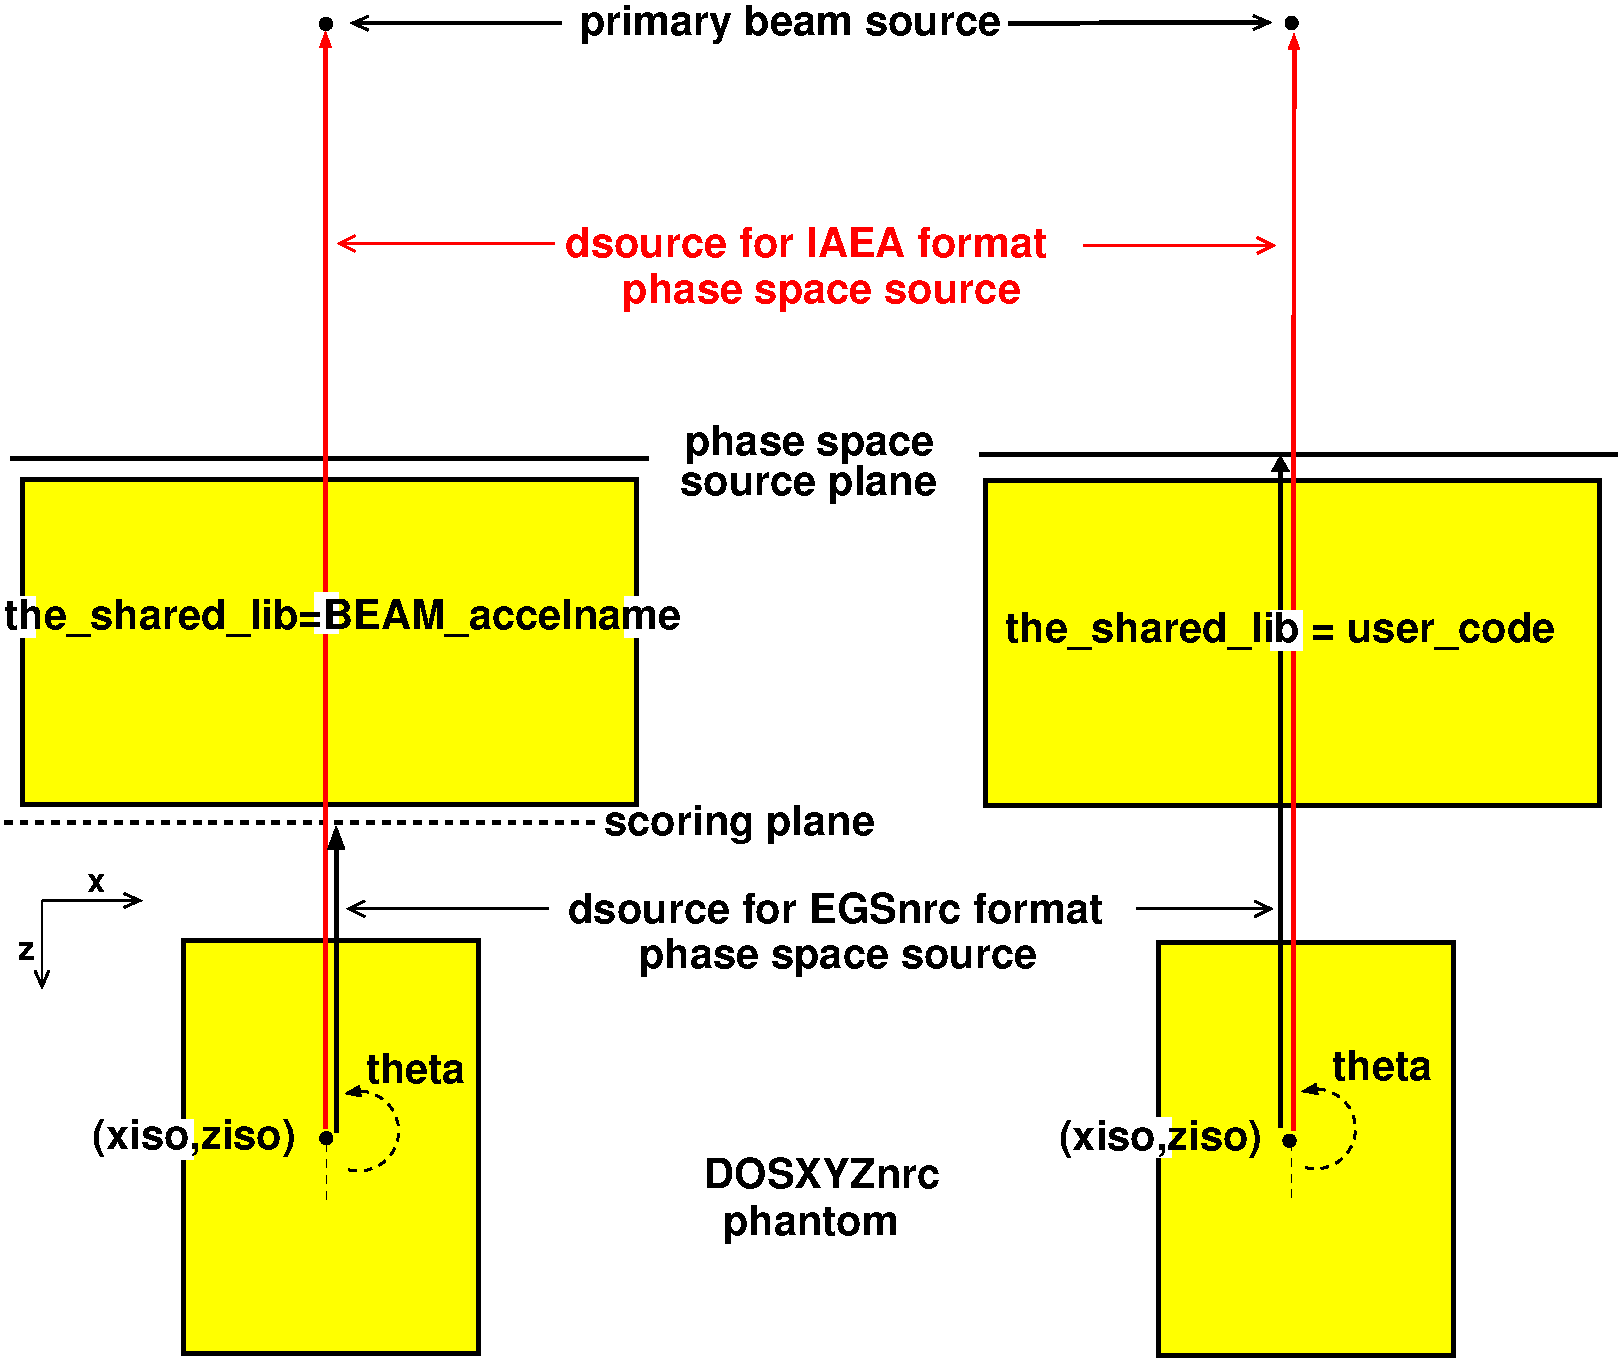
\includegraphics[width=17cm]{figures/src20_1}
\caption{Source 20 incident through a shared library (BEAM or non-EGSnrc user code).  When
the phase space source is run through a BEAM shared library geometry (left), {\tt dsource} defines
the distance between the centre of the scoring plane at the bottom of the geometry and the isocentre (BEAMnrc
phase space source, black arrow), or the distance between the primary source and the isocentre (IAEA phase
space source, red arrow).
When a non-EGSnrc code is used (right), {\tt dsource} defines the distance between the phase space source
and the isocentre (EGSnrc-format phase space source, black arrow) or between the primary source and the isocentre (IAEA phase space
source, red arrow).}
\label{fig_src20_1}
\end{center}
\end{figure}


If a BEAM shared library is used the following conditions apply:
\begin{itemize}
\item The BEAM input file, {\tt the\_input\_file} must define a scoring plane at the bottom of the geometry.  Particle data
at this plane are not actually output but are stored in an internal array for eventual DOSXYZnrc transport through the
phantom.
\item If the source specified in the BEAM input file is a phase space source, it must not make use of the same phase space file as DOSXYZnrc source 20.  This causes a file opening conflict in some versions of
Fortran and will cause the run to fail.  Note that when BEAM is used to define a geometry
for source 20, the BEAM source is not used, so a dummy source of any type can be specified in the BEAM input
file.
\item With a BEAMnrc-format phase space source, the incident Z-position (in the BEAM frame) of the phase space source is
the same as the incident Z-position of the source as defined in the BEAM input file, {\tt the\_input\_file}.  The source 20 input,
{\tt dsource} then defines the distance from the phantom isocentre to the centre of the scoring plane.
\item If an IAEA-format phase space source is used, the incident Z-position of the phase space source is read from
the phase space data itself.  Note that this means the user must ensure consistency between the geometry defined in
BEAM and the incident Z-position of the particles.  The input parameter, {\tt dsource}, defines the distance from
the isocentre to the primary beam source ({\tt i.e.} {\tt dsource}=SAD, see red arrow in figure)
\item The pegs data used in the accelerator simulation is not an input variable and must be the
same as that used in the DOSXYZnrc phantom.
\end{itemize}

If the phase space source is run through a non-EGSnrc shared library (compiled from {\tt user\_code})
the following applies:
\begin{itemize}
\item Phase space data below the defined geometry need not be scored.
\item If a BEAMnrc-format phase space source is used, the incident Z-position (in the {\tt user\_code} frame) is defined
as {\tt dsource}.  Thus, the user must ensure that the source plane is positioned correctly relative to the
defined geometry.
\item For an IAEA-format phase space source, the incident Z-position is read from the phase space source, and
{\tt dsource} defines the primary source-to-isocentre distance.  Again, the user must ensure consistency
between the incident Z-position and the dimensions of the geometry defined in {\tt user\_code}.
\end{itemize}

\indexm{source 20!NRCYCL}
\indexm{source 20!survival ratio}
One issue when running source 20 through a shared library is the determination of how many times
to recycle incident particles so that the phase space source does not rewind, causing loss of information
about particle correlations and subsequent underestimation of dose uncertainties.  As mentioned in Section~\ref{nrcycl}
below, DOSXYZnrc automatically estimates the number of times to recycle each particle, {\tt NRCYCL}, based on
the number of particles in the phase space source, the number of histories requested, and the charge of particles
requested.  However, interactions in the shared library geometry will change the number of particles reaching
the DOSXYZnrc phantom per particle incident from the phase space source.  Thus, the original estimate of
{\tt NRCYCL} is incorrect.  To overcome this when a BEAM shared library is used, an initial calibration comprising
1x10$^6$ particles run through the BEAM geometry only is used to determine the ratio of the number of particles
emerging from the bottom of the BEAM library geometry to the number of incident particles (survival ratio).
{\tt NRCYCL} is then recalculated by multiplying the original estimate by 1/(survival ratio).

\indexm{calflag}
Depending on the shared library geometry, the calibration run can consume
significant CPU time at the beginning of the simulation.  Therefore, if there is a sufficient number of particles in
the phase space source that the user is confident rewinding the source is not an issue, the calibration run can
be skipped by setting the input, {\tt calflag}, to 1.

If a
non-EGSnrc shared library
is used, then the user must provide a routine to estimate the survival ratio of particles passing through the
geometry.  This will be covered in more detail below.

\indexm{synchronized CMs}
When a BEAM shared library geometry includes synchronized component modules (CMs), such as SYNCJAWS, SYNCVMLC or SYNCMLCE,
then the opening coordinates of these component modules (defining the field) can be synchronized with the orientation of the phase space source
plane relative to the phantom.  In this case the value of {\tt MU\_RND}, used to set the incident source orientation (see above), is passed from
DOSXYZnrc to BEAM, where it is then used to set the opening coordinates of any synchronized CMs.
The user controls the synchronization between CM geometries and the incident source orientation using files (one for
each synchronized CM) that associate a field (set of opening coordinates) with a range of fractional monitor units.
See the BEAMnrc Users Manual\cite{Ro09} for more information
about synchronized CMs.

{\bf Non-EGSnrc Geometry Code ({\tt user\_code})}

\indexm{load\_vculib.c}
\index{particleDMLC}
The coding which allows a non-EGSnrc user code compiled as a shared library to communicate with
DOSXYZnrc is found in the C code, {\tt \$HEN\_HOUSE/cutils/load\_vculib.c}. The acronym ``vcu'' stands for
``Virginia Commonwealth University'' and is a reference to the fact that the Lobo and Popescu\cite{LP10}
used a simplified MLC geometry simulation developed at VCU, called {\tt particleDMLC}\cite{Si02}, as a shared
library geometry in simulations with source 20.

\indexm{non-EGSnrc shared library}
\indexm{non-EGSnrc shared library!system requirements}
System requirements for the use of a non-EGSnrc shared library with source 20 (or 21)
are the same as those for a
BEAM simulation source (see Section~\ref{src9sect} above).  Unix/Linux systems must have
a working C/C++ compiler so that {\tt load\_vculib.c} can be compiled to create the
object file, {\tt load\_vculib.o}.  If a working C/C++ compiler is detected on installation
of BEAMnrc/DOSXYZnrc then this is done automatically.  Windows systems do not require
a working C/C++ compiler, since a precompiled version of {\tt load\_vculib.o} is provided.
In addition, the file,
{\tt \$HEN\_HOUSE/specs/dosxyznrc\_config.spec}, where {\tt config} is the configuration
name, must have the
variable {\tt VCULIB\_OBJECTS} set to {\tt \$HEN\_HOUSE/lib/config/load\_vculib.o}
(note that a short form for this is {\tt \$EGS\_LIBDIR/load\_vculib.o})
prior to compiling DOSXYZnrc.  Again, this is set automatically on installation if
{\tt load\_vculib.o} was created successfully.

Currently, {\tt load\_vculib.c} is optimized for calls to subroutines defined in {\tt particleDMLC}. However,
the user can make changes to this file so that it is specific for calls to their own geometry code.  For illustrative
purposes, the following functions must be defined in the user's geometry code, assuming they have made
no changes to {\tt load\_vculib.c} or the DOSXYZnrc coding:

\begin{enumerate}
\indexm{initvcu}
\item{\bf \tt initvcu(char *the\_input\_file, float *survival\_ratio)}
An initialization routine which reads an input file for the geometry code ({\tt the\_input\_file}) and generates
an estimate of the survival ratio of particles between the phase space source and the bottom of the user code
geometry (usually a simulation of an MLC).  The input file would likely specify the geometry parameters and
would also pass the name of the phase space source to the user code.
The survival ratio is used to calculate the number of
times to recycle incident particles, {\tt NRCYCL} (see above).
\indexm{vculib\_sample}
\item{\bf \tt vculib\_sample(float *e, float *x, float *y, float *z, float *u, float *v, float *w, float *wt, int *iq,
 int *latch, int *nhist, int *more\_in\_container)}
A subroutine used to run the geometry code and sample particles reaching the bottom of the geometry.
The subroutine returns the phase space data for a particle at the bottom
of the geometry ({\tt e}=energy; {\tt x,y,z}=particle x,y,z-position; {\tt u,v,w}=x,y,z-direction cosines;
{\tt wt}=particle weight; {\tt iq}=charge; {\tt latch}=latch value), the number of primary histories
run to that point, {\tt nhist}, and an integer, {\tt more\_in\_container}, which is set to 0 if the storage
array for particles reaching the bottom of the geometry is empty ({\tt i.e.} the geometry simulation must
be run on the next call to {\tt vculib\_sample}).
\indexm{vculib\_finish}
\item{\bf \tt vculib\_finish()}
A subroutine called at the end of the simulation to close any files used by the geometry code, free up
reserved memory, etc.
\end{enumerate}

\indexm{source 20!IAEA phase space source}
\label{src20iaeasect}
\subsubsection{IAEA-format phase space sources}

Similar to other phase space sources (sources 2 and 8) source 20 is implemented such that if an IAEA-format phase space source is used, the
incident Z-position of
a particle is automatically read directly from the phase space data.  This eliminates the restriction imposed by BEAMnrc-format
phase space files of all particles being incident in the same plane and, thus, allows more flexibility
in terms of the phase space data that can be used.

\indexm{MU}
\indexm{MU\_RND}
If the IAEA phase space source includes the fractional monitor unit index, {\tt MU}, associated with each particle ({\it i.e.} 4-D data), then
a random value for {\tt MU}, {\tt MU\_RND}, is not chosen at the beginning of each history, and, instead, the value of
{\tt MU} read from the phase space data is automatically
used to set the incident source parameters (isocentre position, incident angle, etc) for the incident particle.
{\tt MU} is automatically
scored in IAEA phase space data output by BEAMnrc simulations using synchronized component modules (CMs) with time-varying opening coordinates
(see the BEAMnrc Users Manual\cite{Ro09}) and can also be included in IAEA phase space data output by DOSXYZnrc
simultions using synchronized sources (20 or 21) by using the {\tt i\_muidx\_out} input flag
(see description of input above and Section~\ref{phspoutsect}).  Thus, use of {\tt MU} read from
the phase space source allows synchronization of source 20 with upstream BEAMnrc simulations having synchronized
CMs or upstream DOSXYZnrc simulations with synchronized sources.

\indexm{spiral CT scan}
\subsubsection{Simulation of Spiral CT Scan}

A recent publication by Kim et al\cite{Ki13} details a modification of Source 8 (See Section~\ref{src8sect} above)
in which the phase space plane can be made to rotate in {\tt phi} about an isocentre which is concurrently
translating in Z, thus simulating exposure in a helical pattern.  Kim et al have used this to simulate dose due
to a spiral CT scan, and their results compare well with measurement.

Spiral scans can be modeled equally well using Source 20 (and 21, see below) using just two control points ({\tt nset}=2).
An example of two control points defining a spiral scan is:

\begin{verbatim}
0, 0, 0, 90, 0, 0, 15, 0
0, 0, 10, 90, 3600, 0, 15, 1.0
\end{verbatim}

These control points define simultaneous translation of the isocentre from {\tt z(1)}=0 to {\tt z(2)}=10 cm and rotation of the source plane
from {\tt phi(1)}=0 at {\tt z(1)} through {\tt phi(2)}=3600$^o$ at {\tt z(2)}.  The angular range, {\tt phi(2)}-{\tt phi(1)}, determines the
pitch of the helix.  In this example, the source rotates ten times (3600$^o$=10$\times$360$^o$) over a Z translation of 10 cm, so the pitch is
equal to 1.  The direction of rotation is determined by the sign of {\tt phi(2)}-{\tt phi(1)}.
If this is positive (as in this example), then rotation is clockwise about the Z-axis; if negative, rotation is counter-clockwise.  Note that the X- and Y-positions of the isocentre in this example remain unchanged, and {\tt theta} is fixed
at 90$^o$, which means the source-isocentre vector is perpendicular to the Z-axis.

The two control points in this example cover the entire range of fractional monitor units ({\it i.e.} {\tt muIndex(1)}=0, {\tt muIndex(2)}=1.0), and, thus,
include all incident particles.
However, using more control points to further subdivide the range, $[$0,1$]$, of fractional monitor units, it would be
possible to generate multiple spiral scans--having different pitch, Z-range, etc--in one simulation.

\subsection{isource = 21: Synchronized BEAM Simulation Source}
\label{src21sect}
\indexm{source routines!isource = 21}
\indexm{source routines!Synchronized BEAM Simulation Source}

Source 21 defines a BEAM treatment head simulation (compiled as a shared library) source incident over multiple ranges
of continuous motion with respect to angle, SSD and isocentre.  The source motion can be synchronized with the settings
of any synchronized component modules (CMs) in the accelerator.  There is also an option to run the source through
a geometry (usually MLC) defined by a non-EGSnrc user code, compiled as a shared library, placed between the treatment
head and the DOSXYZnrc phantom.  Source 21 was developed and contributed by Lobo and Popescu\cite{LP10}.  Just as
source 20 represents a significant enhancement over source 8 (phase space incident from multiple angles), source 21
represents a significant enhancement over source 10 (treatment head incident from multiple angles).

\indexm{source 21!system requirements}
The system requirements for running shared library sources are given in Section~\ref{src9sect} describing source 9 (BEAM
treatment head source incident from one direction).  Instructions on compiling a BEAM accelerator as a shared library
are also given there.

The input parameters for source 21 are:

\begin{description}
\item [~~~~{\tt iqin}]
\indexm{iqin}
Charge of the incident beam (-1: electron, 0: photon, 1: positron, 2: all particle types)
\item [~~~~{\tt isource}] = 21
\item [~~~~{\tt nset}]
\indexm{nset}
\indexm{\$MXANG}
The number of control points defining ranges of continuous source motion.  Same as for source 20 (see above).
{\tt nset} must be in the range 2 $\leq$ {\tt nset} $\leq$ {\tt \$MXANG}, where
{\tt \$MXANG} is defined in
the file {\tt \$EGS\_HOME/dosxyznrc/dosxyznrc\_user\_macros.mortran}.
\item [~~~~{\tt i\_dbs}]
\indexm{i\_dbs}
Set to 1 if directional bremsstrahlung splitting is used in the BEAM simulation and you wish
to reject photons directed outside the splitting field (which will all be fat). Set to 0 otherwise. Note that
{\tt i\_dbs} is read in as a real and converted to integer.
\item [~~~~{\tt e\_split}]
\indexm{e\_split}
Number of times to split charged particles as soon as they enter the phantom geometry. Split particles have their weight reduced by a factor of 1/{\tt e\_split}. This is only used in conjunction with photon splitting ({\tt n\_split}, see Section 8.16) to prevent higher-weight contaminant electrons from compromising statistics in photon beams. For maximum efficiency, it is suggested that you set {\tt e\_split=n\_split}, the photon splitting number.
\item [~~~~{\tt i\_muidx\_out}]
\indexm{i\_muidx\_out}
Set to 1 to include the fractional monitor unit index, {\tt MU}, associated with each particle in IAEA format phase
space output for particles leaving the phantom geometry.  Note that phase space data is not output at all
unless
\indexm{i\_phsp\_out}
{\tt i\_phsp\_out}, the input parameter in the main code controlling phase space output, is set to 1 or 2.
If {\tt MU} is included in the phase space output, then phase space data has a time dimension and is considered 4-D.
Scoring of {\tt MU} allows synchronization between the DOSXYZnrc simulation generating the file and any
downstream simulations--such as BEAMnrc simulations with synchronized component modules--using the file as
a source. See Section~\ref{phspoutsect} for a description of DOSXYZnrc phase space output.
\end{description}

For control points i=1,2,...,{\tt nset}, the following parameters defining the source orientation are entered:
\begin{description}
\item[~~~~{\tt xiso(i)/yiso(i)/ziso(i)}]
\indexm{xiso,yiso,ziso}
x-, y-, z-coordinates of the phantom isocenter.
\item[~~~~{\tt theta(i)}]
\indexm{theta(i)}
Angle of normal connecting origin of the BEAM scoring plane to the isocentre.
\item[~~~~{\tt phi(i)}]
\indexm{phi(i)}
Angle of normal connecting the origin of the BEAM scoring plane to isocentre relative to the +X axis.
\item[~~~~{\tt phicol(i)}]
\indexm{phicol(i)}
2D Angle of rotation of the BEAM scoring plane about its own origin.
\item[~~~~{\tt dsource(i)}]
\indexm{dsource(i)}
The length of the normal from the origin of the BEAM scoring plane to the isocentre.
\item[~~~~{\tt muIndex(i)}]
\indexm{muIndex(i)}
A monitor unit index in the range $[$0,1$]$ defining the fraction of the total number of incident primary histories
delivered up to control point i.  This is slightly different from source 20, where {\tt muIndex(i)} defines the fraction
of incident particles up to control point i.  Thus, for source 21, {\tt muIndex(i)} is actually related to the fractional
monitor units delivered by the BEAM simulation.
Note that {\tt muIndex(i)} $\geq$ {\tt muIndex(i-1)}. Also note that for correct selection of the range
of incident source parameters, {\tt muIndex(1)=0.0} and {\tt muIndex(nset)=1.0}.
\end{description}
This is the end of inputs required for each control point.

\begin{description}
\item[~~~~{\tt the\_beam\_code}]
\indexm{the\_beam\_code}
The name of the BEAM accelerator code ({\it i.e.} {\tt BEAM\_accelname}) used to run the treatment head
simulation.  This must have been compiled as shared library ({\it e.g.} {\tt libBEAM\_accelname.so} on a Linux/Unix system) existing
in your {\tt \$EGS\_HOME/bin/config} directory.
\item[~~~~{\tt the\_input\_file}]
\indexm{the\_input\_file}
The input file for the BEAM treatment head simulation.  This must exist in directory {\tt \$EGS\_HOME/BEAM\_accelname} and must
specify a single scoring plane (usually at the bottom of the accelerator).
\item[~~~~{\tt the\_pegs\_file}]
\indexm{the\_pegs\_file}
The PEGS data to be used in the BEAM treatment head simulation.
\indexm{the\_vcu\_code}
\item[~~~~{\tt the\_vcu\_code}]
This optional input is the name of a non-EGSnrc user code, compiled as a shared library, that can be used to define a geometry
through which particles are run between the bottom of the treatment head and the DOSXYZnrc phantom.  The shared library must
exist in directory {\tt \$EGS\_HOME/bin/config}
\indexm{the\_vcu\_input\_file}
\item[~~~~{\tt the\_vcu\_input\_file}]
Input file for {\tt the\_vcu\_code} defining the geometry interposed between the treatment head simulation and the phantom.
\end{description}

\indexm{\tt MU\_RND}
For each primary history in the treatment head simulation a random fractional monitor unit index, {\tt MU\_RND}$\in[$0,1$]$, is
chosen.  {\tt MU\_RND} is either generated by DOSXZYnrc or, if there are synchronized CMs in the treatment head simulation also
undergoing motion, it is passed to DOSXYZnrc from the BEAM simulation.  More details on the use of synchronized CMs in the BEAM
simulation are given below.  For all particles associated with a given value of {\tt MU\_RND}, the control points, i-1 and i,
within which the source position falls are those for which {\tt muIndex(i-1)}$\leq${\tt MU\_RND}$<${\tt muIndex(i)}, and the
parameters determining the source orientation are calculated using Equation (1) (see Section~\ref{src20sect} above).
Note that, unlike source 20, {\tt MU\_RND} is chosen only for each primary history, not for each incident particle.  Thus,
the {\tt muIndex(i)} for the control points are traceable to actual monitor units in the treatment head.

Recall that the source plane is actually the phase space scoring plane in the BEAM treatment head, defined in {\tt the\_input\_file}.
Phase space data is not output at this plane but is stored in an internal array for use by DOSXYZnrc over the course of the
simulation.

\indexm{i\_dbs}
Similar to source 9 (See section~\ref{src9sect}), since the BEAM simulation is running
concurrently with DOSXYZnrc, if directional bremsstrahlung splitting (DBS) is being used
in BEAM, information about whether or not a particle has been split or has survived
russian roulette (``fat'' particles) is available without having to reconstruct the DBS splitting
field after the fact.  Thus, fat photons can be rejected from the DOSXYZnrc simulation simply
by setting {\tt i\_dbs}=1 and the additional inputs required to reject fat photons from
phase space sources,  {\tt r\_dbs}, {\tt ssd\_dbs}, {\tt z\_dbs} (See Section~\ref{src20sect})
are not required.

\indexm{enflag}\indexm{mode}\indexm{zlast}
As with other phase space and BEAM simulation sources, the input {\tt enflag} must be set
to 2 or 3 to indicate whether {\tt LATCH} bit filtering is to be used, the mode of the
data (with or without {\tt zlast}) being read from the BEAM simulation must be indicated, and
the medium and thickness of the medium surrounding the phantom ({\tt dsurround}) must be
input.  For more information on these inputs, see Section~\ref{sec5}.

\indexm{source 21!use of synchronized CMs}
\subsubsection{Use of synchronized CMs in the BEAM simulation}

If the BEAM treatment head simulation includes synchronized component modules, such as SYNCJAWS, SYNCVMLC, and SYNCMLCE, and
the user is modeling dynamically-changing field coordinates with them, then {\tt MU\_RND} for each primary history is passed
from BEAM to DOSXYZnrc, and the user can synchronize the orientation of the source plane with the field coordinates through
the {\tt muIndex(i)} of the individual control points.  Synchronized CMs are also synchronized with each other.  For more information
on the synchronized CMs, see the BEAMnrc Users Manual\cite{Ro09}.

Figure~\ref{src21_fig} below shows visually how the incident source orientation may be synchronized with the CM settings.

\begin{figure}[htbp]
\begin{center}
\hspace*{-1cm}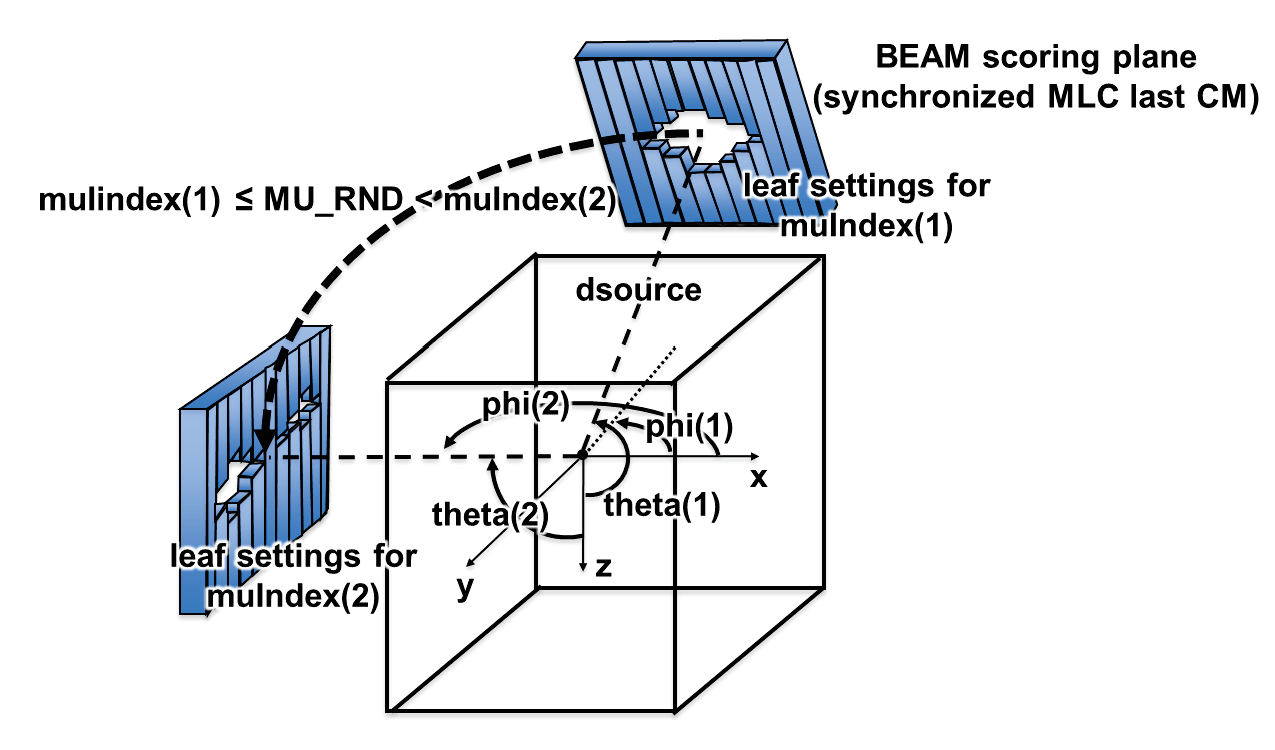
\includegraphics[width=18cm]{figures/src21_fig}
\caption{Source 21, including a synchronized CM, incident on a DOSXYZnrc phantom.  The figure indicates that the final CM in the treatment head
simulation is a synchronized MLC (SYNCVMLC, SYNCMLCE or SYNCHDMLC).  Two control points for the source plane, having different
{\tt muIndex}, {\tt theta} and {\tt phi}, are
indicated.  Different MLC leaf settings are also associated with the values of {\tt muIndex} (the user sets this up in
a file read by the synchronized CM).  Continuous motion of the source between ({\tt theta(1), phi(1)}) and ({\tt theta(2), phi(2)}), along
with dynamic motion of the MLC leaves,
is simulated for values of {\tt MU\_RND} with {\tt muIndex(1)}$\leq${\tt MU\_RND}$<${\tt muIndex(2)}.  Continous motion in
{\tt dource}, isocentre position ({\tt xiso, yiso, ziso}), and the angle of rotation of the source plane in the plane ({\tt phicol}) can
also be simulated.}
\label{src21_fig}
\end{center}
\end{figure}

\indexm{source 21!and non-EGSnrc shared library}
\subsubsection{Running the source through a non-EGSnrc shared library}

\indexm{the\_vcu\_code}\indexm{the\_vcu\_input\_file}
Using the inputs {\tt the\_vcu\_code} and {\tt the\_vcu\_input\_file} the user has the option to interpose another geometry
(usually an MLC) between the source plane and the DOSXYZnrc phantom.  In general, {\tt the\_vcu\_code} is a non-EGSnrc user
code.  Lobo and Popescu\cite{LP10} have used a version of the code particleDMLC\cite{Si02}, developed at Virginia Commonwealth University (hence ``vcu'' in the variable names), to place a simplified MLC simulation between the source and the phantom.

A detailed discussion of potential user codes for creating simplified MLCs is beyond the scope of this manual.  However,
a summary of the subroutines that must exist in {\tt the\_vcu\_code} and the parameters required to communicate
with DOSXYZnrc is given in the description of source 20 (Section~\ref{src20sect}) above.

Note that with source 21, {\tt dsource} always defines the Z-position, in the BEAM frame, of the source plane (scoring plane in the BEAM simulation), and
it is up to the user to ensure that the source is positioned correctly relative to the geometry
defined by {\tt the\_vcu\_code}.


\rfoot[{\sffamily \rightmark}]{{\sffamily \leftmark}}

\section{Other Source-Related Inputs}
\label{sec5}
After the inputs described above, there is another record input with
several other variables related mostly to the source.

\indexm{enflag}
\subsection {{\tt enflag}}
\label{enflag_sect}
The setting of {\tt enflag} determines whether the source is monoenergetic
or has an energy spectrum, or, if the source is a phase space file, whether
or not a dose component is to be calculated.
The possible settings of {\tt enflag} are:
\begin{description}
\item [~~~~= 0] (default) for a monoenergetic source ({\tt isource}=0,1,3,6).
\item [~~~~= 1] for an energy spectrum input ({\tt isource}=0,1,3,6).
\item [~~~~= 2] for a phase space source ({\tt isource}=2) or
full BEAM simulation source ({\tt isource}=9), no dose component
calculation.
\item [~~~~= 3] for a phase space source ({\tt isource}=2) or
full BEAM simulation source ({\tt isource}=9), dose component
calculation using a bit filter (see section~\ref{bitfiltersec} below).
\item [~~~~= 4] for a beam characterization model source ({\tt isource}=4).
\end{description}

\subsection {{\tt mode}}
\indexm{mode}
{\tt mode} only has meaning for a phase space source ({\tt isource}=2).
However, an explicit value for {\tt mode} must exist in the input file
for a full BEAM simulation source ({\tt isource}=9) or
beam characterization model source ({\tt isource}=4), since
{\tt isource}=4 and 9 make use of {\tt medsur}, {\tt dflag} and {\tt dsurround},
which occur after {\tt mode} on the same line.
The possible settings of {\tt mode} are:
\begin{description}
\item [~~~~= 0] (default) the phase space source does not contain
{\tt ZLAST} (for photons, Z of last site of interaction; for electrons,
Z where electron or its ancestor was set in motion by a photon) and, thus,
has 7 variables/record.
\item [~~~~= 2] the phase space source contains {\tt ZLAST} and, thus,
has 8 variables/record.
\end{description}

Note that DOSXYZnrc does not make use of {\tt ZLAST}, but it needs to know
whether {\tt ZLAST} is in the file or not so that the appropriate number
of variables/record can be read.  Thus, if a phase space file is only
going to be used as a source for a DOSXYZnrc calculation, you can save space
by leaving {\tt ZLAST} out of the file.  For more information
about {\tt ZLAST}, see the BEAMnrc Users Manual\cite{Ro09}.

\subsection {{\tt medsur}}
\indexm{medsur}
{\tt medsur} is the medium number for the region surrounding the phantom
as defined by {\tt dsurround}
(see below).  {\tt medsur} is only input for phase space, full BEAM
simulation or beam characterization
model sources ({\tt isource}=2, 4, 8 or 9).  The default setting of {\tt medsur}
is 0, indicating the
surrounding region is vacuum.  However, the user may set this to correspond
to any of the media that they have defined at the top of the DOSXYZnrc input file.
In many cases, the user may wish to fill this region with air and have particles
transported properly through air before reaching the phantom.

\subsection{{\tt dsurround} and {\tt dflag}}
\label{dflagsect}
\indexm{dsurround}
\indexm{dflag}

{\tt dsurround} and {\tt dflag} are required for phase space, full
BEAM simulation and
beam characterization model sources {\tt isource}=2, 4, 8, 9, 10, 20 or 21.
These inputs define the dimensions of the region surrounding the phantom
(ie filled with the medium defined by {\tt medsur}).  Note that
{\tt dsurround} is a 4-dimensional array
with {\tt dsurround(1)} occurring before {\tt dflag} on the input line
and {\tt dsurround(2...4)}, if required, occurring after {\tt dflag}.

The possible settings for {\tt dflag} and their relation to {\tt dsurround}
are as follows:

\begin{description}

\item [~~~~{\tt dflag}=0] (default) {\tt dsurround(1)} defines the thickness
if the surrounding region (in cm) on all sides of the phantom, and the user
need not
input values for {\tt dsurround(2...4)}.  {\tt dsurround(1)}
defaults to 50 cm if it is set $\leq$0.
\item [~~~~{\tt dflag}=1] means that {\tt dsurround(1)} defines the thickness of the
surrounding region in the $\pm$x directions, {\tt dsurround(2)} is the
thickness of the surrounding region in the $\pm$y directions, {\tt dsurround(3)}
is the thickness in the +z direction (bottom of the phantom)
and {\tt dsurround(4)} is the thickness
in the $-$z direction (top of the phantom).  {\tt dsurround(1...4)} default to 0.
\end{description}

Use of {\tt dflag}=1 with {\tt dsurround(1...4)} can save substantial amounts of
computing time if the user is only interested in the dose along a certain axis
or in a specific slice of a DOSXYZnrc phantom (see section~\ref{dsurround_section}
below).

\subsection{{\tt ein}}
\indexm{ein}

{\tt ein} is the kinetic energy of
a monoenergetic incident beam in MeV.  It defaults to 1.25 MeV if
{\tt ein} is set $\leq$ 0.  Note that {\tt ein} is only required if
{\tt isource}=0,1,3,6 and {\tt enflag}=0.

\subsection{{\tt FILNAM}}
\indexm{FILNAM}

{\tt FILNAM} is the file name (with extension) of:

\begin{description}
\item[incident beam energy spectrum] if {\tt isource}=0,1,3 or 6 and
{\tt enflag}=1.  In this case, {\tt FILNAM} has a specific format which
corresponds to the ensrc format used in the original EGSnrc system
\indexm{energy spectrum format}
(see {\tt \$HEN\_HOUSE/spectra} for a large number of
example spectra):

{\tt ENSRC.V5 File format\\
====================}
\begin{tabbing}
\= {\tt SPEC\_TITLE} \\
\> {\tt NENSRC, ENMIN, IMODE} \\
\> {\tt ENSRCD(I), SRCPDF(I) (I = 1 to NENSRC)} \\
\end{tabbing}
\vspace*{-5mm}
where:
\vspace*{-3mm}
\begin{description}
\item [~~~~{\tt SPEC\_TITLE}] is an 80-character spectrum title
\item [~~~~{\tt NENSRC}] = \# of energy bins in the spectrum histogram
\item [~~~~{\tt ENMIN}] = lower energy of first bin in MeV
\item [~~~~{\tt IMODE}] Set to 0 for histogram counts/bin; set to 1 for
counts/MeV
\item [~~~~{\tt ENSRCD(I)}] = upper energy of bin I in MeV
\item [~~~~{\tt SRCPDF(I)}] = probability of finding a particle in bin
I (SRCPDF
need not be normalized)
\end{description}

\item[phase space source:] if {\tt isource}=2 or 8 and {\tt enflag}=2 or 3.
See Section~\ref{source2sect} for more details.
\item[beam characterization model:] if {\tt isource}=4 and {\tt enflag}=4.
\indexm{the\_beam\_code}
\indexm{the\_input\_file}
\indexm{the\_pegs\_file}
\item[{\tt the\_beam\_code}, {\tt the\_input\_file}, {\tt the\_pegs\_file}:]
if {\tt isource}=9 or 10 and {\tt enflag}=2 or 3.  These are the names of the
BEAM accelerator code being used as a source, the input file for the BEAM
simulation, and the pegs data for the BEAM simulation respectively.  See
section~\ref{src9sect} for more details.
\end{description}

\subsection{{\tt IOUTSP}}
\indexm{IOUTSP}
{\tt IOUTSP} is only required with an incident energy spectrum ({\tt enflag}=1).  The
possible settings of {\tt IOUTSP} are:

\begin{description}
\item [~~~~= 0] (default) no output summary of incident energy spectrum
in {\tt .egslst}.
\item [~~~~= 1] output a summary of the incident energy spectrum to the
{\tt .egslst} file.
\end{description}

\section{Phase Space Sources}
\index{phase space sources}

The phase-space files output by BEAMnrc and used by DOSXYZnrc for sources 2 and 8 are
described in detail in section 7 of the BEAMnrc User's Manual.
\cite{Ro04a}.

The phase-space files are binary files  opened with ACCESS = 'direct' and
FORM = 'unformatted'.  Because they are binary files, and because there
are two common byte orders used for binary files by different systems
(eg PCs and DEC machines use one form and SUNs and SGIs use the other),
files written by one system may not be compatible with another system.
The utility {\tt readphsp} found on {\tt \$OMEGA\_HOME/progs/readphsp} can
convert files from one format to the other (see the description in the BEAMnrc
User's Manual. \cite{Ro04a}.)

There are also two types of phase-space files determined by how many
variables they contain.  The shorter format is
called '{\tt MODE0}' and  {\tt ZLAST} is not
scored and the longer format is
'{\tt MODE2}' when {\tt ZLAST} is present.  Since DOSXYZnrc makes no use of
the {\tt ZLAST} variable, it saves space to use {\tt MODE0} files for use with
DOSXYZnrc.  The '{\tt MODE0}' or '{\tt MODE2}'
designation appears in the first record of a phase-space file along
with the total number of particles contained in the file, the number
of photons, maximum energy of any particle in the file,
minimum energy of electrons, and minimum energy of
photons.

\indexm{phase space sources!negative energy marker}
\indexm{phase space sources!using old files}
\indexm{uncertainties}
\indexm{statistics}
Phase space files generated by BEAMnrc use negative
{\tt E} (energy) to mark the first particle scored by each new primary
history.  If the file is used as a source, then the negative {\tt E} marker
allows scored quantities (ie energy deposited) to be grouped according
to primary history.  This ensures that uncertainties estimated account
for the correlations between incident particles in a phase space
source~\cite{Wa02a}.  If an old phase space file without negative {\tt E} markers is used
as a source, then scored quantities will be grouped according to incident
particle instead of primary history.  DOSXYZnrc will then output a warning
that uncertainty may be underestimated because correlations between incident
particles could not be taken into account.  This is not a cause for concern,
because we have found~\cite{Wa02a} that in the cases we studied,
the underestimate is not significant.

When using a phase space source, if the entire phase space file is read
before the requested number of histories is run, then DOSXYZnrc restarts
the phase space file from the beginning.  For the reasons discussed in
section~\ref{nrcycl}, page~\pageref{nrcycl}, this is not a desirable
occurrence and one should strive to avoid this by using the recycling
feature (which also saves on reading time).

\index{IAEA-format phase space sources}
\label{iaeaphspsect}
\subsection{IAEA-format Phase Space Sources}

In addition to the standard BEAMnrc phase space files described
above, DOSXYZnrc can
also use IAEA-format phase space data as a source.  This allows the
user to make use of IAEA's online data base of accelerator phase space
data at:\\
\htmladdnormallink{www-nds.iaea.org/phsp/phsp.htmlx}{http://www-nds.iaea.org/phsp/phsp.htmlx}

\index{C++ compiler}
Note that this functionality requires that EGSnrc/DOSXYZnrc be installed on a machine
with a working C++ compiler.  This is detected automatically during
EGSnrc installation and, if a working C++ compiler is found, the library
of IAEA phase space handling routines is compiled.

\index{{\tt .IAEAheader}}
\index{{\tt .IAEAphsp}}
\index{IAEA phase space data! header file}
\index{IAEA phase space data! phase space data file}
Phase space data in IAEA format comprises both a header
(extension {\tt .IAEAheader}) file and a phase space data
(extension {\tt .IAEAphsp}) file.  When using IAEA phase space data as
a source, only the full name and directory path of the {\tt .IAEAphsp} file needs to be specified
(See Section~\ref{source2sect}).  The {\tt .IAEAheader} file is assumed to be
in the same directory.

Note that when IAEA phase space sources are used the incident Z-position of each particle
is available and is automatically read, either from the header file in the case of
planar phase space data (such as that scored by BEAMnrc), or from the phase space
data itself if it is scored in 3-D (such as that scored by DOSXYZnrc).  The ability to handle
3-D phase space data greatly enhances the flexibility of DOSXYZnrc and allows it to
use non-planar data supplied by manufacturers, such as that supplied by Varian for
their TrueBeam accelerators.  In addition, IAEA phase space files generated by BEAMnrc simulations
with synchronized component modules (CMs) and by DOSXYZnrc simulations using synchronized
sources (20 or 21) may include the fractional monitor unit ({\tt MU}) associated with each particle.
This is automatically read in and used by DOSXYZnrc's synchronized phase space source (source 20) allowing
synchronization between the DOSXYZnrc simulation and the upstream simulation that generated the phase
space file.  See Sections~\ref{src2iaeasect} and \ref{src20iaeasect} for more information.

Form more information on the format of IAEA phase space data, see the
BEAMnrc Manual and IAEA Report INDC(NDS)-0484\cite{CJ05}.

\section{Calculating Dose Components with DOSXYZnrc}
\label{bitfiltersec}
\subsection{Bit Settings}
\indexm{bit setting}

\indexm{LATCH}
The {\tt LATCH} variable, associated with each particle in a
BEAMnrc simulation, is a
32-bit variable used to track the particle's history.  It is discussed in
detail in the BEAMnrc User's Manual \cite{Ro04a}.

Each bit in {\tt LATCH} is designated as follows with bit 0 being the lowest value bit:
\begin{description}
\item [~~~~bit 0] Set to 1 if a photon is created by a bremsstrahlung event or an electron is created by a bremsstrahlung photon; 0
otherwise
\item [~~~~bits 1-23] Used to record the region where a particle has been and/or
has interacted. Note that the bit set for a region is determined by
{\tt IREGION\_TO\_BIT} (which is defined in the BEAMnrc simulation)
for that region.
\item [~~~~bits 24-28] Stores {\tt IREGION\_TO\_BIT} (as a binary number) of the
region in which a secondary particle
is created; if these bits are all 0, the particle is a primary
particle
\item [~~~~bits 29-30] Store the charge of a particle at the time {\tt LATCH} is output
\indexm{LATCH}
to a phase-space file.
\item [~~~~bit 31] Set to 1 if a particle has crossed a scoring plane
more than once when {\tt LATCH} is output to a phase-space file.
\indexm{LATCH}

\end{description}

For secondary particles, recording the {\tt IREGION\_TO\_BIT}'s of
the regions in which they were
created in bits 24-28 is equivalent to multiplying the {\tt IREGION\_TO\_BIT} by
2$^{24}$, or 16777216.  Thus, to retrieve {\tt IREGION\_TO\_BIT} of the region
of origin of a
secondary particle, the {\tt LATCH} value of the particle must be divided by
16777216 (i.e., taking the value {\tt INT(LATCH/16777216)}).
\indexm{LATCH}

When used with a phase space source, DOSXYZnrc has the
capability of selecting from the phase space file only those particles that
have user-specified bits (called a ``bit filter") set in their {\tt LATCH}
variables.
Thus, DOSXYZnrc will score only the dose component arising from these user-selected
particles.  For example, in the BEAMnrc simulation, bit 10 may be associated
with a square applicator, so any particle in the phase space file that has
been in the applicator will have bit 10 set in {\tt LATCH}.  When using
this phase space file as a source in DOSXYZnrc, the user may opt to use only
those particles that have bit 10 set, thus scoring the dose component from
particles that have been in the applicator.

In general, a dose component can be selected
according to what regions particles have passed through/interacted in,
whether the particle is a primary or secondary, if the particle is a
secondary then where it was created, and any combination of these.

\subsection{Input for Dose Component Calculations}

In order to enable dose component calculations with a phase space source
or full BEAM simulation source
({\tt isource}=2, 8 or 9),
the variable {\tt enflag} must be set to 3.  The user then specifies which
\indexm{enflag}
type of bit filter ({\tt I\_BIT\_FILTER}) to use.  Below is a description of the
4 types of bit filters available and the inputs associated with each.

\begin{description}
\indexm{I\_BIT\_FILTER}
\indexm{NBIT1}
\indexm{NBIT2}
\indexm{BIT}
\index{IREGION\_TO\_BIT}
\item [{\tt I\_BIT\_FILTER}=0] This is an inclusive/exclusive bit filter.  On the
same line as {\tt I\_BIT\_FILTER}, the user inputs the integers {\tt NBIT1} and
{\tt NBIT2}.  {\tt NBIT1} is the number of bits to include and {\tt NBIT2} is
the number of bits to exclude.  Restriction is that
0$\leq${\tt NBIT1}+{\tt NBIT2}$\leq$29.
Both {\tt NBIT1} and {\tt NBIT2} can be set to zero.  On the next line, the
user inputs {\tt BIT(I) (I=1,NBIT1)}, the bits to be included, and on
the following line \\ {\tt BIT(I) (I=NBIT1+1,NBIT1+NBIT2)}, the bits to
be excluded.  If any of the first set of {\tt NBIT1} bits are set and none
of the second set of {\tt NBIT2} bits are set in the particle's {\tt LATCH}
variable, the particle is used in the
simulation.

\item [{\tt I\_BIT\_FILTER}=1] This is an exclusive bit filter.  On the same line
as {\tt I\_BIT\_FILTER}, the user inputs the integer {\tt NBIT1}, the
number of bits to be excluded (0$\leq${\tt NBIT1}$\leq$29).  {\tt NBIT2} is
not relevant for this filter and is automatically set to 0.  On the
next line, the user inputs, {\tt BIT(I) (I=1,NBIT1)}, the bits to
be excluded.  If any of these {\tt NBIT1} bits are set in the particle's
{\tt LATCH} variable, the particle
is NOT used in the simulation.

\item [{\tt I\_BIT\_FILTER}=2] An inclusive region-of-origin filter.
The user inputs {\tt NBIT1} on the same line
as {\tt I\_BIT\_FILTER}, where {\tt NBIT1} is the number of regions of origin
to be included.  Since regions of origin are distinguished only by their
values of {\tt IREGION\_TO\_BIT}, {\tt NBIT1} can also be seen as the
number of distinct values of {\tt IREGION\_TO\_BIT} to be included. The
restriction on {\tt NBIT1} is 0$\leq${\tt NBIT1}$\leq$24.  {\tt NBIT2} is
not relevant for this filter and is automatically set to 0.  On the
next line, the user inputs {\tt IREGION\_TO\_BIT(I) (I=1,NBIT1)}, the
{\tt IREGION\_TO\_BIT} values of the {\tt NBIT1} regions of origin to
be included.  If the particle originated in any one of these {\tt NBIT1}
regions, then it will be used in the simulation.  Primary particles will be included if
{\tt IREGION\_TO\_BIT=0} is one of the {\tt NBIT1} values of
{\tt IREGION\_TO\_BIT} to include.

\item [{\tt I\_BIT\_FILTER}=3] An exclusive region-of-origin filter.
The user inputs {\tt NBIT1} (0$\leq${\tt NBIT1}$\leq$24), the number of
regions of origin to be excluded, on the same line as {\tt I\_BIT\_FILTER} and
ignores {\tt NBIT2}, since it is not relevant for this filter.  On the
next line the user inputs {\tt IREGION\_TO\_BIT(I) (I=1,NBIT1)}, the
{\tt IREGION\_TO\_BIT} values of the regions of origin to be excluded.
If a particle originated in any one of these regions, then it is NOT
used in the simulation.  Note that primary particles will be excluded if
{\tt IREGION\_TO\_BIT=0} is one of the {\tt NBIT1} values of
{\tt IREGION\_TO\_BIT} to exclude.

\end{description}

Note that since only one bit filter can be input per simulation, only one
dose component may be calculated at a time using DOSXYZnrc.  This is because
of the large memory requirements for the dose scoring arrays.

\section{Other Input Variables}

This section provides descriptions of main DOSXYZnrc input variables not
covered above.

\vspace*{-0.5cm}
\subsection{{\tt IPHANT}}
\label{iphantsect}
\indexm{IPHANT}

If {\tt IPHANT} is set to 1, DOSXYZnrc outputs phantom data to
a {\tt .egsphant} file.  This file has the same format as the
{\tt .egsphant} file that {\tt ctcreate} outputs for CT data
(see section~\ref{egsphantsect}) and can be read by
{\tt dosxyz\_show}\cite{Ka98},
along with the {\tt .3ddose} dose output file to display isodose contours in
the phantom.  Note that this option is redundant (and, therefore, unavailable)
when using a CT phantom because it is an input file from ctcreate).

\subsection{{\tt MAX20}}
\indexm{MAX20}
\label{MAX20description}

When {\tt MAX20} is set to 1, a summary of the maximum 20 doses in the
phantom is output to the screen (log file) and list file.  This summary
includes an output of the 20 maximum doses with their fractional
uncertainties and coordinates, the average of the 20 maximum doses, the average
fractional uncertainty of these doses (not the uncertainty of the average), the
average fractional uncertainties of all doses $>$ 50\% of the maximum dose,
and the average absolute uncertainty of all doses $>$ 50\% of the maximum dose
as a fraction of the maximum dose.

When not in CT phantom mode, {\tt MAX20} is the last variable on the line(s)
specifying the regions for which dose will be output (ie record 9).  If
{\tt MAX20} is set to 1 on ANY ONE of these lines (including the line of
zeros indicating the end of this record) then the summary of the 20 maximum
doses will be output.

In CT phantom mode, {\tt MAX20} is input
\indexm{MAX20} on the same line as {\tt zeroairdose} and {\tt doseprint}.

This option is useful for timing/efficiency studies.
\subsection{{\tt zeroairdose}}
\indexm{zeroairdose}
\label{zeroairdose}

{\tt zeroairdose} is only used in CT phantom mode.
Setting {\tt zeroairdose} to 1 will set all dose estimates in
voxels with density $<$ 0.044 g/cm$^3$ to zero in the {\tt .3ddose}
\indexm{.3ddose}
\indexm{files!.3ddose}
file.  This has the effect of zeroing dose in voxels filled with air
(see the default CT ramp in Figure~\ref{fig_ct02}--note that ``AIR''
has a density ranging from 0.001-0.044 g/cm$^3$).
Air dose will not be zeroed in the {\tt .egslst} file, this file will
continue to report the precise estimated dose.  {\tt zeroairdose} serves
as a dose visualisation parameter for CT phantom simulations, since, in general, the user is only interested
in seeing the dose within the patient, not in the surrounding air.

\subsection{{\tt doseprint}}
\indexm{doseprint}

This input parameter is also only used in CT phantom mode.

{\tt doseprint} is set to 1 if the user wants a full output of doses in
all voxels of the CT phantom in the {\tt .egslst} file.  Since, in CT
phantom cases, the user is usually not interested in this output and, owing
to the large number of voxels in a CT phantom, it can make the {\tt .egslst}
exceptionally large, the default is to suppress this output (ie set
{\tt doseprint} to 0).

\subsection{{\tt NCASE}}
\indexm{NCASE}

{\tt NCASE} is the number of histories to run in a simulation.  Minimum
value is 100.  Default is 100 if {\tt NCASE} is set $<$ 100.  The number
of histories per output batch is equal to {\tt NCASE}/({\tt \$NBATCH}),
where {\tt \$NBATCH} is currently set to 10.

\subsection{{\tt IWATCH}}
\indexm{IWATCH}

{\tt IWATCH} controls output to the screen (interactive run) or to the
{\tt .egslog} file (batch run) during beam execution.  The possible settings
are:
\begin{description}
\item [~~~~= 0] (default) On completion of each batch, outputs information about the
batch (eg elapsed time, CPU time, elapsed/CPU time, random number used
to begin batch, \# of random seeds used in the batch, total number of
histories run up to and including the current batch, the total number of
particles scored in the first phase-space file)

\item [~~~~= 1] Outputs same information as 0 plus, after every particle
interaction, outputs complete information about the particle(s)
involved (eg interaction type, particle type, position of particle on
stack, particle energy, X-Y-Z position of particle, U-V-W direction
cosines, {\tt LATCH} value of particle, region \# of particle); also informs
\indexm{LATCH}
user when a particle is being discarded, when a particle is passing from
one CM to another

\item [~~~~= 2] Similar to 1 but with complete particle information output at
every step; also outputs total dose in a region whenever energy is
deposited there

\item [~~~~= 3] Similar to 2 but with particle and dose information output
whenever dose is deposited.

\item [~~~~= 4] Outputs same information as 0 plus {\tt .egsgph} and {\tt
.egsgeom} files for graphical representation of the accelerator and
particle paths using {\tt EGS\_Windows.}
\indexm{.egsgph}
\indexm{.egsgeom}
\indexm{files!.egsgph}
\indexm{files!.egsgeom}
\end{description}

\subsection{{\tt TIMMAX}}
\indexm{TIMMAX}

{\tt TIMMAX} is the maximum CPU time in hours allowed for a simulation.
{\tt TIMMAX} defaults to 0.99 hrs if it is set = 0.  However, this time-restriction function is not activated in the current version of DOSXYZnrc except to
print a warning as it starts a batch which will exceed this limit.


\subsection{{\tt INSEED1, INSEED2}}
\indexm{INSEED}
\indexm{RANMAR}
\indexm{RANLUX}
\indexm{random number generator}
\indexm{random number seeds/pointers}

These are random number seeds used to initialize the
RANMAR\cite{MZ91,Ma90a} or RANLUX\cite{La94,Ja94}
random number generator.  Within DOSXYZnrc,
{\tt INSEED1} is limited
to the range\\ 0$<${\tt INSEED1}$\leq$31328
(defaults to 1802), and {\tt INSEED2} has
the range 0$<${\tt INSEED2}$\leq$30081 (defaults to 9373).  These
ranges/defaults are designed for RANMAR (the default random number generator),
however, if
you are using RANLUX then {\tt INSEED1} is the ``luxury level"
of the random number generator and must be in the range
0$<${\tt INSEED1}$\leq$4, otherwise, it will automatically be set to the
default luxury level of 1 (Note: this means that the DOSXYZnrc default value
for {\tt INSEED1} of 1802 will ultimately get reset to 1 by RANLUX).

Note that \verb+INSEED1+ and \verb+INSEED2+ are only used to initialize
the random number generator, and, during a simulation, they no longer
reflect the values of the seeds that are actually used to generate
the random numbers.
During restarts
({\tt IRESTART} = 1), the state of the random number generator at the end
of the previous run is read from the {\tt .egsdat} file and is used at the
beginning of the restart.
Thus, a restarted run with a total of
10000+10000 histories should generate results identical to a single run
of the same simulation with 20000 histories.  Also note that
when running parallel jobs
with DOSXYZnrc (see section~\ref{parallelcalc}), {\tt INSEED2} must have
a different value for each of the individual jobs that make up the simulation.
This is taken care of automatically if you use DOSXYZnrc's built-in
parallel processing functionality.

\index{random number generator! switching from RANMAR to RANLUX}
In order to switch from the RANMAR random number generator to RANLUX in
DOSXYZnrc, go into {\tt \$EGS\_HOME/dosxyznrc/Makefile} and
change the line:
\begin{verbatim}
RANDOM = $(EGS_SOURCEDIR)ranmar
\end{verbatim}
to:
\begin{verbatim}
RANDOM = $(EGS_SOURCEDIR)ranlux
\end{verbatim}
Then recompile DOSXYZnrc.

\subsection{{\tt BEAM\_SIZE}}
\indexm{BEAM\_SIZE}

{\tt BEAM\_SIZE} allows user control of incident beam size for sources 2 and
8 (phase-space input), 9 and 10 (full BEAM simulation sources) and 4
(beam model source). {\tt BEAM\_SIZE} is the side of a square field in cm. The default value for {\tt BEAM\_SIZE} is 100 cm. When phase-space particles are read from a
data file or reconstructed by a multiple-source model, DOSXYZnrc will check their positions and discard those that fall outside of the specified field.

One should be careful with the use of this parameter because particles outside
the specified field (defined by {\tt BEAM\_SIZE)} may have some effects on the dose
distributions calculated and therefore the results may be biased with the use
of {\tt BEAM\_SIZE} smaller than the field size of the original phase-space data. It
should also be noted that this parameter cannot be used as a beam defining tool,
such as a collimator,
because in reality particles outside of the inner opening of any beam confining
components may interact with and be scattered by the components,  resulting in
an increase of the particles within the specified field.

\subsection{{\tt ISMOOTH}}
\label{ismooth}
\indexm{ISMOOTH}

\indexm{re-use of phase space}
When phase-space data are used DOSXYZnrc will re-use the phase-space particles if
\indexm{phase-space input}
the number of histories required by the user is greater than the number of
particles stored in the phase-space file. Clearly, the dose distributions
obtained with more histories have smaller statistical uncertainties.
Although some histories may start with the same incident phase-space, the
particle trajectories will be different because different random numbers will
be used in the simulations in the phantom, resulting in different dose
distributions. However, surface doses are mainly affected by the electron
fluence distribution and therefore would not be improved by re-using the
phase-space particles if the data file contains too few particles
(i.e., the calculated doses
would have small statistical uncertainties but large systematic uncertainties).

In order to reduce the systematic uncertainties due to a small data set,
DOSXYZnrc can re-distribute the phase-space particles {\bf as long as the
simulated linear accelerator geometry is symmetric,  and the treatment
field is centred on the beam axis}. Currently, DOSXYZnrc is allowed to move a
particle  to 3 symmetrical positions (each with modified direction
cosines). This process is accurate as long as the phase space file is
symmetric with respect to the x-axis and also with respect to the
y-axis.  Suppose a particle is at (x,y) with (u,v) the 3 new positions
are
\begin{center}
(-x,y) with (-u,v), \\
(x,-y) with (u,-v), \\
(-x,-y) with (-u,-v)
\end{center}
%%Dave commented the following out since even after corrections, he
%is not at all convinced it is right.
%If further, their is a square symmetry (eg if no jaws are included in the
%simulated linear accelerator geometry or they are all on the same level),
%one can further move the particle
%to 4 other positions (one needs to modify DOSXYZnrc in order to do so), i.e.,
%
%\begin{center}
%
%(x,y) with (-u,-v),
%
%(-x,y) with (u,-v),
%
%(x,-y) with (-u,v),
%
%(-x,-y) with (u,v)
%\end{center}
A user has two options for {\tt ISMOOTH}:
\indexm{ISMOOTH}
\begin{description}
\item [~~~~= 1] DOSXYZnrc re-distributes the phase-space particles when they are used more than once.


\item [~~~~= 0] (default) DOSXYZnrc re-uses the phase-space particles without changing the particle positions

\end{description}
\indexm{re-use of phase space}

See also section~\ref{nrcycl} which discusses recycling phase space data.

\subsection{{\tt NRCYCL}}
\label{nrcycl}
\indexm{NRCYCL}
\indexm{phase space source!recycle}

{\tt NRCYCL} is an essential input when using a phase space source. It
determines the number of times that each particle from a phase space
source is recycled ({\em  ie}, reused each time it is read).
If {\tt NRCYCL}$>$0, then
each source particle is used a total of {\tt NRCYCL} + 1 times
before moving on to the next particle in the source.
When phase space data is sparse, then particles must be re-used to obtain
adequate statistics.  In addition to recycling, particles may also
be re-used whenever a phase space source is restarted
(happens automatically when the simulation has reached
the end of the source).  Restarting is not recommended, however,
because it may lead to underestimates of the uncertainty in the
final results~\cite{Wa02a}.  We recommend setting {\tt NRCYCL} to a value
that will ensure that the entire phase space source gets sampled (ie
the simulation uses almost all the particles in the source) but
prevents the source from being restarted.

If you are unsure of
the correct value of {\tt NRCYCL} to use, then
run with {\tt NRCYCL}=0 and DOSXYZnrc will automatically calculate
a value of {\tt NRCYCL} based on the number of histories and
the number of particles (with appropriate charge) in the phase space source.
There is a possibility
that, even with the automatically calculated value of {\tt NRCYCL},
the phase space source will restart.  This may be due to particles
that have been rejected because they missed the geometry, were multiple
passers and/or were beyond the beam field defined by {\tt BEAM\_SIZE}) or
else the algorithm for calculating {\tt NRCYCL} may have determined that
setting {\tt NRCYCL}$>$ 0 will result in the phase space source not being
sampled adequately.
If the
source has only been restarted once and only a small fraction of it
has been covered on the second pass, this is not likely to have a significant
impact on the estimated uncertainties.  However, if a large portion of the
source is covered on the second pass, or if it is restarted more than once,
we recommend re-running the simulation with a new value of
{\tt NRCYCL} calculated as:
\begin{eqnarray}
\label{nrcycleqn}
{\tt
NRCYCL}=
\frac{{\tt NCASE}}{\left({\tt NPHSP - (NSMISS/NRCYCL}_{prev}) - {\tt NOUTSIDE - NRJCT - NDBSRJCT}\right)}-1
\end{eqnarray}
where {\tt NCASE} is the number of incident histories, {\tt NPHSP} is the
total number of particles in the phase space file, {\tt NSMISS} is
the number of particles that missed the geometry in the previous run,
{\tt NRCYCL$_{prev}$} is the setting of {\tt NRCYCL} in the previous run,
{\tt NOUTSIDE} is the number of particles rejected because they were
outside the field defined by {\tt BEAM\_SIZE} in the previous run,
{\tt NRJCT} is the number of particles rejected because they were
multiple passers in the previous run, and {\tt NDBSRJCT} is the number of
photons rejected because they fall outside the directional bremsstrahlung
splitting (DBS) field radius at the SSD (only if DBS was used in the BEAM
simulation that generated this source AND the user has opted to reject
these photons--see section~\ref{source2sect} for more information about
this).  Note that {\tt NPHSP}, {\tt NSMISS}, {\tt NOUTSIDE},
{\tt NRJCT} and {\tt NDBSRJCT} are all available from the {\tt .egslst} file of the previous run.
Always round your calculated value of {\tt NRCYCL} up to the nearest integer.
\indexm{DBS}
\indexm{NRCYCL}

{\tt NRCYCL} is not automatically calculated if you are only using the
positrons in the phase space source or if you are selecting a sub-set of
the phase space source based on {\tt LATCH} settings.  In these cases,
the information required for an a-priori calculation of {\tt NRCYCL}
is not available in the header of the phase space source.
We recommend setting {\tt NRCYCL} manually to a ``best guess" value.  Then,
if the source restarts, calculate {\tt NRCYCL} using Equation~\ref{nrcycleqn}
where {\tt NRJCT} includes the number of particles rejected because they
were multiple passers, the number of particles rejected because they were
the wrong charge and the number of particles rejected because they did not
have the right {\tt LATCH} setting.

If the phase space source is stored on a remote disk, then using
{\tt NRCYCL} to avoid restarting a phase space source also has
the beneficial effect of reducing network traffic
because it reduces the number of times that a phase space
source is accessed during a run (particle data is stored in temporary
variables during recycling, not re-read from the source).  Repeated
accessing of a phase space source on a remote disk can slow a simulation
down considerably.

{\tt NRCYCL} is compatible with {\tt ISMOOTH} (see section~\ref{ismooth}).
So if {\tt ISMOOTH}=1, then,
during the recycling loop, the initial position and direction cosines of
the particle are shifted according to the scheme outlined in the
{\tt ISMOOTH} subsection above.
\indexm{ISMOOTH}
\indexm{NRCYCL}

Note that the total number of histories is
always limited by {\tt NCASE}.  For example, if the
phase space source has 1000 suitable particles and the user sets {\tt NRCYCL}=9
(so each particle will be used a total of 10 times), but only sets
{\tt NCASE}=5000, then the simulation will only have a chance to use (and
recycle) the first 500 particles before the simulation stops.  In order to
go through the entire phase space source, the user would have to set
{\tt NCASE}=10000.  If {\tt NCASE}$>$10000 then the phase space source
would be restarted at least once during the run.  After restarting, particle
recycling continues as before.

\subsection{{\tt IRESTART}}
\label{irestartsect}
\indexm{IRESTART}
\indexm{restarting}

\indexm{.egsdat}
The possible settings of {\tt IRESTART} are:
\begin{description}
\item [~~~~= 0] (default) DOSXYZnrc initiates a new run, deleting all of the output
files ({\tt .egslog,} {\tt .egslst}, {\tt .egsdat}, \etc) if present
\item [~~~~= 1] Restart of a previous run; DOSXYZnrc opens the
{\tt .egsdat} from the previous run and reads:
\begin{enumerate}
\item $\sum_{i=1}^{nhist}edep_i$ and $\sum_{i=1}^{nhist}edep_i^2$ for
all voxels, where {\tt edep$_i$} is energy deposited by primary (non-phase space)
history i
and {\tt nhist} is the number of primary histories in the previous run.
\item number of histories and number of primary histories from the previous run
\item the time taken by the previous run
\item the state of the random number generator at the end of the
previous run
\item other data relating to particle fluence in previous run, number of
electron steps, number of particles rejected from phase space source (if
applicable), etc.
\end{enumerate}
After the current run is complete, dose and
uncertainties are calculated using data from the current run and from
the previous run~\cite{Wa02a}.  Note that the
number of histories to run and the total CPU time allowed for the
simulation do not include the histories and CPU time from the previous run.
Also note that, currently, although a restarted simulation with, for example
100000+100000 histories will have identical dose results to a one-off
simulation
with 200000 histories, the uncertainty estimates on the doses may not be
the same.  We are currently investigating why this is so.
\item [~~~~= 2] DOSXYZnrc creates the {\tt .egsinp} file and then exits without
running the simulation
\item [~~~~= 3] DOSXYZnrc opens the {\tt .egsdat} file from a previous run,
reads the data enumerated above and calculates doses and uncertainties;
no simulation is run.
\indexm{.pardose}
\item [~~~~= 4] DOSXYZnrc recombines the binary {\tt .pardose} files from
parallel jobs and creates {\tt .egslst} and {\tt .3ddose} output
files from the recombined data (see section~\ref{parallelcalc} for
more about parallel jobs).
\end{description}

\subsection{{\tt IDAT}}
\label{idatsect}
\indexm{IDAT}
\indexm{files!.egsdat}
\indexm{.egsdat}

The possible settings of the variable {\tt IDAT} are:
\begin{description}
\item [~~~~= 0] (default) DOSXYZnrc outputs {\tt .egsdat} file with
restart data after every batch.
\item [~~~~= 1] DOSXYZnrc does not output a {\tt .egsdat} file at all.
\item [~~~~= 2] DOSXYZnrc outputs a {\tt .egsdat} with restart data only at
the end of the entire run.
\end{description}
For large phantoms, writing this file will take a lot of time. For
production runs use 2 usually.

\subsection{{\tt IREJECT}}
\indexm{IREJECT}

{\tt IREJECT} is a switch for turning on charged particle range
rejection.  Range rejection can save simulation time by terminating
\indexm{range rejection}
particle histories immediately if they cannot reach
the boundary of the current voxel with energy $>$ {\tt ECUT} and their
current energy is less than {\tt ESAVE\_GLOBAL}. This is the same as the
{\tt IREJECT\_GLOBAL} = 2 option in the BEAMnrc code as discussed in the
BEAMnrc User's Manual \cite{Ro04a}.
\indexm{range rejection}
\indexm{ESAVE\_GLOBAL}
\indexm{ECUT}

The possible settings of {\tt IREJECT} are:
\indexm{IREJECT}

\begin{description}
\item [~~~~= 0] (default) DOSXYZnrc will not perform charged particle range
rejection.
\item [~~~~= 1] DOSXYZnrc will immediately terminate the history of a
charged particle and deposit its remaining energy in the current voxel
if its energy is $<$ {\tt ESAVE\_GLOBAL} (see description
in next section) and if it cannot reach the nearest voxel boundary with
an energy $>$ {\tt ECUT}.
\indexm{ESAVE\_GLOBAL}
\indexm{ECUT}
\end{description}

It is found that for 5~mm$^3$ voxels, range rejection can save 10 to 17\%
on computing time but for smaller voxels it saves less time (3 to 4\%
for 2.5~mm$^3$ voxels).  For non-CT phantoms where one can arrange to
have at least some of the voxels quite large, the savings will be
correspondingly larger, especially using the dsurround option
(see section~\ref{dsurround_section}).

Similar to BEAMnrc, range to {\tt ECUT} is determined by subtracting
the range from {\tt ECUT} to {\tt AE} (determined using EGSnrc macros and
EGSnrc-calculated tables of range to {\tt AE} as a function of particle
energy) from the particle's {\tt range} to {\tt AE} (calculated in EGSnrc)
at every charged particle step.  Rejection of particles based on
range to {\tt ECUT} is performed by a DOSXYZnrc macro and
not by the EGSnrc's built-in range rejection macro.  This
is because the EGSnrc range rejection is based on range to
{\tt AE} and not {\tt ECUT}.
\indexm{range rejection}

\subsection{{\tt ESAVE\_GLOBAL}}
\indexm{ESAVE\_GLOBAL}

{\tt ESAVE\_GLOBAL} is the maximum energy (in MeV) for which range rejection
\indexm{range rejection}
calculations will be performed (ie a particle cannot be rejected if its
energy is $\geq$ {\tt ESAVE\_GLOBAL}).  This option is to prevent
termination of high-energy electrons which are likely to generate
bremsstrahlung.
\indexm{range rejection}

\subsection{{\tt n\_split}}
\label{nsplitsect}
\indexm{n\_split}
\indexm{photon splitting}

{\tt n\_split} is used to control DOSXYZnrc's photon splitting option.
If {\tt n\_split} is set $>$ 1 all photons are split
into {\tt n\_split} photons, each with a weight equal to
$\frac{1}{{\tt n\_split}}$ times the weight of the original photon.  For each
photon, i, where i=1,2,...,{\tt n\_split}:
\begin{itemize}
\item The mean free path to its next interaction, $DPMFP_i$, given by
\begin{equation}
DPMFP_i=-{\tt ln}\left(1-\frac{\eta+i-1}{{\tt n\_split}}\right)
\end{equation}
where $\eta$ is a random number, chosen once for all {\tt n\_split} photons.
\item At the interaction site, each photon i produces charged particles and/or
scattered
photons.  Russian roulette is played on all scattered photons with a
survival probability of $\frac{1}{{\tt n\_split}}$.  Surviving photons
have their weight increased by {\tt n\_split} so that their weight is equal
to the weight of the
original photon before splitting.  All charged particles survive with weight equal
to $\frac{1}{{\tt n\_split}}$ times the original weight.
\item If these charged particles undergo radiative events (bremsstrahlung,
  annihilation, annihilation at rest), Russian roulette is played on the
  resultant photons with a survival probability of $\frac{1}{{\tt n\_split}}$.  Again,
  surviving photons have their weight increased by {\tt n\_split} so that their
  weight is equal to the weight of the original photon before splitting.
\item Photons whose weight has been restored to the original weight are
  subject to splitting again.
\end{itemize}

Photon splitting has the potential to increase the efficiency of a dose
calculation more than photon interaction forcing.  A good rule of thumb for
the setting of {\tt n\_split} is:
\begin{equation}
{\tt n\_split}>=\frac{N}{1-e^{-\lambda}}
\end{equation}
where $\lambda$ is approximately equal to the number of photon mean free paths
in the geometry of interest and {\tt N} $\geq$ 5.  This will increase the
number of primary interactions per incident photon by approximately {\tt N},
so reduce {\tt NCASE} by a factor of {\tt N}.

\indexm{photon splitting!with phase space sources}
\indexm{photon splitting!with BEAMnrc sim. sources}
It has recently been shown\cite{KW06} that the use of photon splitting
with a phase space source (Section~\ref{source2sect}) or BEAMnrc
simulation source (Section~\ref{src9sect}) can increase
the efficiency of dose calculations in simulated photon beams by
a factor of up to 6.5 (depending on beam energy, field size and phantom
voxel size).  Moreover, the optimum efficiency ({\em i.e.} at the
optimum value of {\tt n\_split}) with a BEAMnrc simulation
source is only 3--13\% lower than that with the corresponding
phase space source, potentially eliminating the need to store
phase space data.  Thus, it is highly-recommended that you use photon
splitting to increase the efficiency of photon beam dose calculations.
The optimum setting of {\tt n\_split} for phase space and BEAMnrc simulation
sources depends
on incident beam energy, field size and phantom voxel size.  For
BEAMnrc simulation sources, splitting numbers of
40 ($0.25\times0.25\times0.25$ cm$^3$ voxels) or 32
($0.5\times0.5\times0.5$ cm$^3$ voxels) should give efficiencies close
to the optimum, and for phase space sources, splitting numbers of
32 ($0.25\times0.25\times0.25$ cm$^3$ voxels) or
24 ($0.5\times0.5\times0.5$ cm$^3$ voxels) will be close to the optimum.
Note that these settings of {\tt n\_split} are higher than those
calculated using the rule of thumb given in the paragraph
above.  This is because much of the efficiency improvement is due to the
fact that {\tt n\_split} reduces the number of source particles required,
thus reducing the CPU time spent generating the source particles
(transport through the jaws in the case of a phase space source,
performing an entire treatment head simulation in the case of a BEAMnrc
simulation source), whereas the rule of thumb is based on the efficiency
improvement being solely due to the efficiency inherent in the
splitting algorithm itself.

\indexm{e\_split}
When {\tt n\_split} is used with a phase space or BEAMnrc simulation
source, then contaminant electrons may compromise dose statistics because
they are fewer and will have a higher weight than the split photons
(which contribute most of the dose).  To avoid this, the phase space
sources ({\tt isource}=2,8) and the BEAMnrc simulation source
({\tt isource}=9) have an input, {\tt e\_split}, which can be used to
split charged particles {\tt e\_split} times as soon as they enter
the phantom geometry.  The weight of the particle is reduced by
1/{\tt e\_split}.  To maximize efficiency, it is recommended that you
set {\tt e\_split}={\tt n\_split} if you
are using photon splitting with a phase space or BEAMnrc simulation source.
For more information about {\tt e\_split} see Sections~\ref{source2sect}
and~\ref{src9sect}.

\subsection{{\tt ihowfarless}}
\label{howfarlesssect}
\indexm{ihowfarless}
\indexm{``HOWFARLESS'' option}

If {\tt ihowfarless} is set to 1, then DOSXYZnrc uses the ``HOWFARLESS''
algorithm for transport in the phantom.

The ``HOWFARLESS'' algorithm is used to significantly increase the
efficiency of dose calculations in a homogeneous phantom.  When the option
is used, the {\tt HOWFAR} and {\tt HOWNEAR} subroutines in DOSXYZnrc only
consider the extreme outer boundaries of the phantom when calculating
the distance along the particle trajectory to the next region boundary
and the perpendicular distance
to the nearest region boundary respectively.  This eliminates the need
to stop at voxel boundaries and, hence, speeds up charged particle
transport considerably.  For the purposes of dose deposition, the
total curved charged particle step is approximated by two straight-line
steps joined at a hinge point.  The straight-line steps can be calculated
based on either the known initial position/direction of the particle
or its known final position/direction.  As coded, the ``HOWFARLESS''
algorithm uses a 1:1 mixture of step approximations based
on the initial position/direction and approximations based on the
final position/direction.  This has been found to give accurate dose
results over all energies and maximum allowed step lengths
(input variable {\tt SMAX}, see paragraph below).

When the ``HOWFARLESS'' option is used, the limitations on step
length within the phantom become the maximum allowable charged particle step length,
{\tt SMAX} (see Section~\ref{smaxsect}), and the maximum fractional
energy loss per electron step, {\tt ESTEPE} (see Section~\ref{estepesect}).
It is recommended that you leave {\tt SMAX} at its default
value (5 cm if you are using the {\tt PRESTA-I} boundary crossing
algorithm or electron step algorithm, 1e10 cm if you are using
the {\tt EXACT} boundary crossing algorithm and the {\tt PRESTA-II}
electron step algorithm).  At most beam energies, this will ensure
that step length is only limited by {\tt ESTEPE}, which it is not
recommended that you change.

The efficiency gained using the ``HOWFARLESS'' algorithm depends on
the source type, energy, field size, phantom voxel size, and the
boundary crossing algorithm (BCA) used.  For a photon beam from a
BEAMnrc-simulated linac (using either a phase space source or
full BEAMnrc simulation source),
use of ``HOWFARLESS'' increases the efficiency by $\sim$30\% when the
{\tt PRESTA-I} BCA is used, and by a factor of 2.5-3.5 when the more
accurate (but much slower) {\tt EXACT} BCA is used.  In the case of
a simple photon beam source ({\em e.g.} a parallel beam simulated using
{\tt isource}=1) with an energy spectrum, the efficiency gain with
``HOWFARLESS'' is a factor of 1.5-2.5 with the {\tt PRESTA-I} BCA
and a factor of 5-9 with the {\tt EXACT} BCA.  The highest efficiency
gains occur in monoenergetic electron beams, where ``HOWFARLESS''
increases the efficiency by a factor of 3-4 with the {\tt PRESTA-I}
BCA and 8-14 with the {\tt EXACT} BCA.  Efficiency gains are much
greater with the {\tt EXACT} BCA because calculations with standard
HOWFAR use the BCA at every voxel boundary, while ``HOWFARLESS''
calculations use the BCA only at the extreme outer boundaries of the phantom.
Thus, the standard calculation becomes much slower when the BCA is
switched from {\tt PRESTA-I} to {\tt EXACT}, while the speed of
the ``HOWFARLESS'' calculation does not decrease appreciably.  For
more information about BCA's see Section~\ref{bcasect}.

Use of ``HOWFARLESS'' is recommended in all homogeneous phantom calculations,
such as those used for beam commissioning.  More information about
this option can be found in the ``HOWFARLESS'' paper by
Walters and Kawrakow\cite{WK06}.

\subsection{{\tt i\_phsp\_out}}
\label{phspoutsect}
\indexm{i\_phsp\_out}
\indexm{writing phase space data}

If {\tt i\_phsp\_out} is set to 1 or 2, DOSXYZnrc outputs phase space data in IAEA format
for particles leaving the phantom geometry.  The phase space data is in 3-D, meaning
that it includes
the (X,Y,Z) position for each particle.  If {\tt i\_phsp\_out}=1, then the particle positions
are in the DOSXYZnrc coordinate system, and if {\tt i\_phsp\_out}=2, the particle positions
are transformed into the BEAMnrc, or source, coordinate system.  Note that phase space
output requires the existence of a region surrounding the phantom geometry and, thus, is limited
to phase space sources (source no.'s 2, 8, 20), BEAMnrc simulation sources (source no.'s 9, 10, 21)
and the multiple source model (source no. 4), all of which require the input of
\indexm{dflag}\indexm{dsurround}
{\tt dflag} and {\tt dsurround} to define the dimensions and medium of a surrounding region
(see Section~\ref{dflagsect}).

\indexm{i\_muidx\_out}
If phase space data is output when source 20 (synchronized phase space source) or 21 (synchronized BEAM simulation
source) is used then, through the {\tt i\_muidx\_out} input for those sources (see Sections~\ref{src20sect} and~\ref{src21sect}),
the user has the option to also include the fractional monitor unit index, {\tt MU}, associated with the particle
in the output phase space data.  Thus, the data includes a time dimension and is considered 4-D. Scoring
4-D data allows simulations downstream of the DOSXYZnrc simulation--{\it e.g.} BEAMnrc simulations with
synchronized component modules or further DOSXYZnrc simulations with synchronized sources--that use the
phase space data as a source to be synchronized with the DOSXYZnrc simulation that generated the phase space
file.

Since it includes the Z-position of each particle, the size of an IAEA phase space file written by
DOSXYZnrc may be slightly larger than that written by BEAMnrc, with the minimum record size (bytes/particle) for
DOSXYZnrc being 33 bytes while that for BEAMnrc is 29 bytes.  If {\tt MU} is included in the phase space
data, then the record size increases to 37 bytes.  Note that DOSXYZnrc does not have an option to
\indexm{ZLAST}
include {\tt ZLAST} (Z position of last site of photon interaction or creation of secondary charged particle) in
the phase space output.

\indexm{phase space file output!naming scheme}
Unlike BEAMnrc, DOSXYZnrc does not have the possibility of defining multiple phase space scoring planes.
Thus, the naming scheme for phase space space files output by DOSXYZnrc does not include the scoring plane
number, and the files are simply named {\tt inputfile.IAEAheader} (header file) and {\tt inputfile.IAEAphsp}
(phase space data).

The default directory for phase space output is {\tt \$EGS\_HOME/dosxyznrc} ({\it i.e.} the user code directory).
The user can change the phase space output directory by editing the file\\
 {\tt \$EGS\_HOME/dosxyznrc/dosxyznrc\_user\_macros.mortran}, changing the macro\\ {\tt \$DIRECTORY-FOR-PHSP} to the name of the desired output directory (include
the full path), and then recompiling DOSXYZnrc.

For more information on the IAEA phase space file format, see the BEAMnrc Users Manual\cite{Ro09}.

\subsection{{\tt i\_bindos}}
\indexm{i\_bindos}
If {\tt i\_bindos} is set to 1, DOSXYZnrc outputs a sparse binary dose file instead of a dense ASCII dose file.
The resulting file typically has a much smaller memory footprint than the default {\tt .3ddose} format.
See section~\ref{subsec:bindos_format} for a description of the format.

\subsection{ECUTIN}
\indexm{ECUTIN}
\label{ECUTIN}
\indexm{ECUT}

\verb+ECUTIN+ is used together with the {\tt Global ECUT} input in the
EGSnrc input parameters (see section~\ref{egsnrc_inputs}) to define the
global electron cutoff energy in MeV.
If {\tt ECUTIN} $>$ {\tt Global ECUT}
in the EGSnrc inputs, or if the {\tt Global ECUT} input is missing from the
EGSnrc inputs, then {\tt ECUTIN} is used as global cutoff energy.

As soon as an electron's total energy falls below the cutoff energy, its
history is terminated and its energy deposited in the current region.
The time required for a given calculation is strongly dependent on the
value of \verb+ECUT+ and thus it is important to use as high a value
as possible.

The user can override
the global \verb+ECUT+ with the \verb+ECUT+'s defined for individual regions within
\verb+CMs+ (see CM descriptions below).  However, if the \verb+ECUT+ for an
individual region is $<$ global \verb+ECUT+, then it is set equal to the
global \verb+ECUT+.

Note that \verb+AE+ for the PEGS4 data set used is the lower limit on
the value of \verb+ECUT+ used in a given region.  The selection of
\verb+AE+ also requires some care and is discussed in section 14 of
the BEAMnrc manual.
\index{AE} \index{ECUT!rule of thumb}

Selection of \verb+ECUT+ is complex in general and is very dependent on
what is being calculated\cite{Ro84,RB90}.  For therapy beams,
\verb+ECUT+ can be quite high since low-energy electrons contribute
little to dose in phantom.  For what we consider detailed work, we have
used \verb+ECUT+ = 0.700 MeV but much higher may be possible.  However,
if the dose in the monitor chamber is an important part of the
calculation, lower values of \verb+ECUT+ may be required.

As a general rule of thumb for calculations of dose distributions,
\verb+ECUT+ should be chosen so that the electron's range at \verb+ECUT+
is less than about 1/3 of the smallest dimension in a dose scoring region.
This ensures energy is transported and deposited in the correct region
although for electrons which are moving isotropically, this can be a
very conservative requirement.

\subsection{PCUTIN}
\indexm{PCUTIN}
\label{PCUTIN}
\indexm{PCUT}

\verb+PCUTIN+ is used together with the {\tt Global PCUT} input in the EGSnrc
input section to define the global cutoff energy for photon transport in
MeV.  It is the photon equivalent of \verb+ECUTIN+.  Similar to {\tt ECUTIN},
if {\tt PCUTIN} is $>$ the value input for {\tt Global PCUT} in the EGSnrc
input section, or if {\tt Global PCUT} is omitted from the EGSnrc inputs, then
{\tt PCUTIN} is used as the global {\tt PCUT}.  Also
the user can override global \verb+PCUT+ with \verb+PCUT+s defined for
individual regions within CMs.

The exact value of the global \verb+PCUT+ is not critical in the sense that low
values do not take much more time. A value of 0.01 MeV
should generally be used.

\subsection{{\tt ESTEPM, SMAX}}
\indexm{ESTEPM}
\indexm{SMAX}

These are dummy inputs that used to define the
maximum fractional energy loss per step ({\tt ESTEPM}) and maximum
step length ({\tt SMAX}).  These transport parameters are now handled in the
EGSnrc inputs.  The dummy inputs have been preserved to ensure compatibility
with EGS4/DOSXYZ input files.

\section{EGSnrc inputs}
\label{egsnrc_inputs}
\index{EGSnrc inputs}

The use of EGSnrc to simulate charged particle and photon transport
in DOSXYZnrc allows the user a greater degree of control over the
transport physics
than was previously available in EGS4 versions of DOSXYZ.  For most
accelerator applications, the DOSXYZnrc default settings of the EGSnrc
parameters should be adequate, however, there are some cases, such
as low-energy applications, in which the user will want to vary
the EGSnrc transport parameters using the EGSnrc inputs.

EGSnrc inputs appear at the end of a DOSXYZnrc input file between the
delimiters {\tt :start mc transport parameter:} and
{\tt :stop mc transport parameter:}.  The format follows that of the
general purpose EGSnrc user-codes\cite{Ro00}.


In general, EGSnrc inputs must appear in the input file in
the format:

{\tt PARAMETER NAME= parameter value}

Note that there is a space between the ``=" sign and the parameter value.
Of course, if you are using the DOSXYZnrc GUI to set the EGSnrc inputs, then
the above format is written to the input file automatically when you save
the input parameters.

If any or all of the EGSnrc input parameters is missing, then the default
setting will be used. This feature allows DOSXYZ input files to be used
directly with DOSXYZnrc. A better approach is to read the old DOSXYZ input
file into the {\tt dosxyznrc\_gui} and then save it since this will explicitly
add the required EGSnrc inputs to the file.

The following sections describe the EGSnrc inputs required in
DOSXYZnrc.  For more information, see the EGSnrc manual\cite{KR00}. The
actual internal variable name associated with each input appears in brackets.

\subsection{ {\tt Global ECUT} ({\tt ECUT})}
\index{Global ECUT}
\index{ECUT}
\index{ECUTIN}

{\tt Global ECUT} defines the global electron cutoff energy ({\tt ECUT})
in MeV.
This is one of the two EGSnrc input parameters that is also accessible
through the main DOSXYZnrc input section of the input file (the other
is {\tt Global PCUT} described below).  Specifically, if {\tt ECUTIN}
in the main
DOSXYZnrc inputs is $>$ {\tt Global ECUT}, or if {\tt Global ECUT} is
missing from the EGSnrc input section, then the global value of
{\tt ECUT} is set to {\tt ECUTIN}.  See section~\ref{ECUTIN} for a more
detailed discussion of {\tt ECUT}.

\subsection{ {\tt Global PCUT} ({\tt PCUT})}
\index{Global PCUT}
\index{PCUT}
\index{PCUTIN}

{\tt Global PCUT} defines the global photon cutoff energy ({\tt PCUT})
in MeV.
Similar to {\tt Global ECUT}, this EGSnrc input parameter is also accessible
through the main DOSXYZnrc input section of the input file.
If {\tt PCUTIN} in the main
DOSXYZnrc inputs is $>$ {\tt Global PCUT}, or if {\tt Global PCUT} is
missing from the EGSnrc input section, then the global value of
{\tt PCUT} is set to {\tt PCUTIN}.  See section~\ref{PCUTIN} for a more
detailed discussion of {\tt PCUT}.

\subsection{{\tt Global SMAX} ({\tt SMAXIR})}
\label{smaxsect}
\index{Global SMAX}
\index{SMAX}
\index{SMAXIR}

{\tt Global SMAX} defines the maximum electron step length in cm.  If the
default EGSnrc electron step electron algorithm (see
section~\ref{essect}) and the exact boundary crossing algorithm are used, then no
restriction on maximum step length is needed.  However, if using
PRESTA-I (the EGS4 standard) as the electron step algorithm or the boundary
crossing algorithm, then
{\tt Global SMAX} must be set to a reasonable value (eg 5 cm) to ensure
proper electron transport in low density materials (air).
{\tt Global SMAX} defaults to 5 cm when PRESTA-I BCA or electron step
algorithm is used is used and 1.E10 cm
when the EXACT BCA and PRESTA-II electron step
algorithm are used.

\subsection{{\tt ESTEPE} ({\tt ESTEPE})}
\index{ESTEPE}
\label{estepesect}

{\tt ESTEPE} is the maximum fractional energy loss per electron step.
For accurate electron transport with default EGSnrc electron
step algorithm (see section~\ref{essect} below) {\tt ESTEPE} should
not exceed 0.25 (the default).  {\tt ESTEPE} should not be changed
unless PRESTA-I is being used as
the electron transport algorithm.

\subsection{{\tt XImax} ({\tt XIMAX})}
\index{XIMAX}

{\tt XIMAX} is the maximum first multiple elastic scattering moment per electron
step.  It is equal to roughly half the average multiple scattering angle
squared.  Make sure you do not set {\tt XIMAX} $>$ 1,
since this is beyond the range of available multiple scattering data.
The default value of 0.5 should be sufficient for most applications.

\subsection{{\tt Boundary crossing algorithm} ({\tt bca\_algorithm})}
\index{boundary crossing algorithm}
\index{bca\_algorithm}
\label{bcasect}

This controls the algorithm used to transport electrons across region
boundaries.  There are two possible settings of
{\tt Boundary crossing algorithm}: {\tt EXACT} and
{\tt PRESTA-I} (the default).  In the {\tt PRESTA-I} case boundary
crossing is carried out in a manner similar to EGS4.  Specifically, lateral
pathlength corrections are turned off if the perpendicular distance
from the electron to the boundary is less than
{\tt Skin depth for BCA} (see
section~\ref{skindepthsect} below) and then, once the electron reaches
the boundary, a multiple scattering event is forced.
If {\tt EXACT} boundary crossing is used, electrons are
transported in
single elastic scattering mode as soon as they are within a distance from
the boundary given by the EGSnrc input {\tt Skin depth for BCA} (see
section~\ref{skindepthsect} below).

The {\tt EXACT} boundary
crossing algorithm was introduced in EGSnrc to eliminate a
known fluence singularity caused by forcing a
multiple scattering event at a boundary~\cite{FS95}.  Although
the {\tt PRESTA-I} BCA can be up to 3 times more efficient than
the {\tt EXACT} BCA it has been shown to result in dose overestimation
by up to 2.5\% in simulations where charged particle equilibrium does not
hold ({\em e.g.} small beam field on voxels with dimensions $\sim$ field
size) or when dose voxels are much smaller than the voxels making up the
rest of the phantom\cite{KW06}.  Under such conditions, you must
manually switch to the {\tt EXACT} BCA for accurate results.

\subsection{{\tt  Skin depth for BCA} ({\tt skindepth\_for\_bca})}
\index{skin depth for BCA}
\index{skindepth\_for\_bca}
\label{skindepthsect}

If {\tt Boundary crossing algorithm= PRESTA-I}, then
{\tt Skin depth for BCA} is the perpendicular distance
(in elastic mean free paths) from the boundary
at which lateral pathlength corrections are turned off and the particle
is transported in a straight line until it reaches the boundary.
By default the distance at which to switch off
lateral corrections is a fixed value calculated by EGSnrc to be
the same as that used in the original implementation of PRESTA in EGS4 and
depends on the value of {\tt ECUT}.

If {\tt Boundary crossing algorithm= EXACT}, then {\tt  Skin depth for BCA}
determines the perpendicular distance (in elastic mean
free paths) to the region boundary
at which electron transport will go into
single elastic scattering mode.  A skin depth of 3 elastic mean free
paths has been found to give peak efficiency in this case and is the
default for this case.

If {\tt Boundary crossing algorithm= EXACT} and
{\tt  Skin depth for BCA} is set to a very large number (eg 1e10),
then the entire simulation will be done in single scattering mode.


\subsection{{\tt Electron-step algorithm} ({\tt transport\_algorithm})}
\label{essect}
\index{electron step algorithm}
\index{transport\_algorithm}

This input determines the algorithm used to calculate lateral and
longitudinal corrections to account for elastic scattering in a condensed
history electron step.  There
are 2 possible settings: {\tt PRESTA-II} (the default) and
{\tt PRESTA-I}.  {\tt PRESTA-II} (the name ``PRESTA" is preserved only
for historical reasons) is the new, more accurate, algorithm developed for
use with EGSnrc\cite{KR00}.  {\tt PRESTA-I} is the original
PRESTA algorithm with some modifications
\cite{BR87,Le50}.  The original {\tt PRESTA-I} is
known to underestimate lateral deflections, to underestimate longitudinal
straggling and to produce a singularity in the distribution describing
the lateral spread of electrons in a single condensed history.
While {\tt PRESTA-I} may be accurate enough for high energies
(where elastic scattering is weak), it is not recommended for low
energy applications.

\subsection{{\tt Spin effects} ({\tt spin\_effects})}
\index{spin effects}
\index{spin\_effects}

If {\tt Spin effects= on} (the default), then elastic scattering
cross-sections that take into account relativistic spin effects are used
in electron transport.  If {\tt Spin effects= off},  then
screened Rutherford cross-sections (similar to EGS4) are used for elastic
scattering.  It should be noted that using {\tt Spin effects= on} does
increase calculation time, however, results are more accurate and it
is ABSOLUTELY necessary for good backscatter calculations.

Including spin effects has a small but distinct effect on calculated
depth-dose curves.  In low-Z materials such as water, the value of
$R_{50}$ for a given energy is higher than with EGS4/PRESTA. For high-Z
materials it is the reverse and backscatter also increases.


\subsection{{\tt Brems angular sampling} ({\tt IBRDST})}
\index{bremsstrahlung angular sampling}
\index{IBRDST}

This input determines the type of angular sampling that is done when
a bremsstrahlung photon is created.   If {\tt Brems angular sampling= Simple}
(the default) then bremsstrahlung angles are sampled using only the leading
term of modified equation 2BS of Koch and Motz\cite{Bi89,KM59}. If
{\tt Brems angular sampling= KM}, then the bremsstrahlung angles are sampled
using the entire modified equation.
{\tt Brems angular sampling= Simple} is adequate at high energies,
however, there is little increase in simulation time associated with using
the entire modified 2BS equation and the entire equation is recommended
at low energies.
Note that {\tt Brems angular sampling= KM} is similar to the bremsstrahlung
angular sampling scheme used by the latest version of EGS4/DOSXYZ, with some
modifications.

\subsection{{\tt Brems cross sections} ({\tt IBR\_NIST})}
\index{bremsstrahlung cross sections}
\index{IBR\_NIST}

This input determines the cross-section used for bremsstrahlung interactions.
If {\tt Brems cross sections= BH} (the default), then Bethe-Heitler cross-sections
(Coulomb corrected above 50 MeV)\cite{KM59} are used.  These cross-sections
are similar to those used by EGS4/DOSXYZ.  If {\tt Brems cross sections= NIST}, then
cross-sections from the NIST bremsstrahlung cross-section data base\cite{SB85,SB86a}
are used.  The NIST cross-sections are the basis for radiative stopping powers
recommended by the ICRU\cite{ICRU37}.  The difference between {\tt BH} and
{\tt NIST} is negligible for energies $>$ 10MeV, but becomes significant in
the keV energy range. There is also
a {\tt Brems cross sections= NRC} option.  The NRC cross-sections
are the NIST cross-sections including corrections for electron-electron
bremsstrahlung (typically only
significant for low values of the atomic number Z and for k/T < 0.005).

\subsection{{\tt Bound Compton scattering} ({\tt IBCMP})}
\index{bound Compton scattering}
\index{IBCMP}
\label{bcsect}

The {\tt Bound Compton scattering} input is used to determine whether binding effects
and Doppler broadening are simulated in Compton (incoherent) scattering
events.  If this input is set to {\tt Off} (the default), then the Klein-Nishina
formula\cite{KN29} is used to determine cross-sections for
Compton scattering.  This is similar to the treatment of Compton scattering
in EGS4/DOSXYZ.  If {\tt Bound Compton scattering= On}, then
the original Klein-Nishina formula is augmented with the
impulse approximation\cite{Ri75} to simulate binding effects and
Doppler broadening.  Simulation of binding effects and Doppler broadening takes
extra time and is only important below 1 MeV and/or if Rayleigh
scattering is being simulated (see section~\ref{rayleighsect}).
A third option, {\tt Bound Compton scattering= Norej}, is provided which
uses the total bound Compton cross sections ({em i.e.} no impulse
approximation) and does not reject any Compton interactions at run
time.

Bound Compton scattering may also be turned on in selected regions
(off everywhere else) using
{\tt  Bound Compton scattering= On in regions} together with
the inputs {\tt Bound Compton start region} and {\tt Bound Compton stop region}
to define the region ranges for which bound Compton is to be turned on.
Conversely, bound Compton can be turned off in selected regions
(on everywhere else) by inputting
{\tt  Bound Compton scattering= Off in regions} with
{\tt Bound Compton start region} and {\tt Bound Compton stop region} used
to define the region ranges where bound Compton is to be turned off.  Of
course, turning bound Compton on/off in regions is accomplished much more
easily in the DOSXYZnrc GUI.  Note that the {\tt Norej} option cannot be
used on a region-by-region basis.

\subsection{ {\tt Compton cross sections} ({\tt comp\_xsections})}
\index{Compton cross section data}
\index{comp\_xsections}

If the {\tt Bound Compton scattering= Norej} option is selected (see above), then
the user also has the option of
specifying their own Compton cross section data
using the {\tt Compton cross sections} input.  Cross section data must exist
in the {\tt \$HEN\_HOUSE/data} directory and the file name must have
the form {\tt x\_compton.data}, where {\tt x} is a name
specified by the user.  All values of {\tt x} will appear in the GUI menu where Compton
cross section data can be selected.  Alternatively, if editing
the {\tt .egsinp} file directly, the form of this input is:
\begin{verbatim}
Compton cross sections= x
\end{verbatim}
Default Compton cross section
\index{Compton cross section data!default}
data, {\tt default\_compton.data}, is included in
the EGSnrc system.

\subsection{{\tt Radiative Compton corrections} ({\tt radc\_flag})}
\index{radiative Compton corrections}
\index{radc\_flag}

If set to {\tt Radiative Compton corrections= On}, then radiative
corrections for Compton scattering based on the equations
of Brown and Feynman (Phys. Rev. 85, p 231--1952) are used.
If set to {\tt Off} (the default) no corrections are done.
Note that if set to {\tt On} then the variable {\tt SOURCES} in
{\tt \$EGS\_HOME/dosxyznrc/Makefile} (See Section~\ref{filesect} above)
must be modified to include {\tt \$(EGS\_SOURCEDIR)rad\_compton1.mortran} just
before {\tt \$(EGS\_SOURCEDIR)get\_inputs.mortran}.

\subsection{{\tt Pair angular sampling} ({\tt IPRDST})}
\index{pair angular sampling}
\index{IPRDST}

This input determines the method used to sample the positron/electron emission
angles (relative to the incoming photon) in a pair production event.  There
are three possible settings of this input: {\tt Off}, {\tt Simple} and {\tt KM}.
If it is set to {\tt Off}, then the positron and electron created by pair
production have fixed polar angles, $\theta_{\pm}$, given by
$\theta_{\pm}=\frac{m}{E_{\gamma}}$, where m is the electron rest energy
and $E_{\gamma}$
 is the energy of the original photon.  This is similar to the method used to determine
positron/electron emission angles in the original version of EGS4.
If {\tt Pair angular sampling= KM}, then eqn 3D-2003 in
Motz et al\cite{Mo69} is used to determine the positron/electron emission
angles.  This option is similar to the sampling technique used by the current
version of EGS4/DOSXYZ.  Finally if {\tt Pair angular sampling= Simple} (the default), then only
the first term in the Motz et al eqn 3D-2003 is used.  The {\tt KM} option
becomes less efficient with increasing accelerator energies and, moreover, involves
assumptions that are questionable at low energy.  For these reasons, the default
setting is {\tt Simple}.


\subsection{ {\tt Pair cross sections} ({\tt pair\_nrc})}
\index{Pair cross sections}
\index{pair\_nrc}

The {\tt Pair cross sections} input determines the cross-sections to
use for pair production events.  If set to {\tt BH} (the default), then
Bethe-Heitler cross sections are used.  If set to {\tt NRC}, then the
NRC cross sections found in {\tt \$HEN\_HOUSE/data/pair\_nrc1.data} are
used.  The {\tt NRC} setting is only of interest at low energies, where
these cross-sections take into account assymmetry in the positron-electron
energy distribution.

\subsection{{\tt Photoelectron angular sampling} ({\tt IPHTER})}
\index{photoelectron angular sampling}
\index{IPHTER}

The {\tt Photoelectron angular sampling} input determines the sampling method
used by EGSnrc to determine the angle of emission of photoelectrons.
If {\tt Photoelectron angular sampling= Off} (the default), then
 photoelectrons inherit the direction of the incident photon.  If
{\tt Photoelectron angular sampling= On}, then Sauter's formula
\cite{Sa31} is used to determine the angle of the photoelectron.  Note
that, in most applications, we have not observed any difference between
the ``Off" and ``On" settings of this parameters.  Also note that,
strictly speaking, Sauter's formula is only valid for K-shell photo-absorption
and is also derived from extreme relativistic approximations.  Thus, if
the user has a better approach, they can insert it in the
{\tt \$SELECT-PHOTOELECTRON-DIRECTION;} macro in
{\tt \$HEN\_HOUSE/egsnrc.macros}.

Similar to bound Compton scattering, photoelectron angular sampling
can be turned on or off in selected regions (with the opposite setting
everywhere else) by setting
{\tt Photoelectron angular sampling= On in regions} or
{\tt Photoelectron angular sampling= Off in regions} together with
the inputs {\tt PE sampling start region} and
{\tt PE sampling stop region} to define the region ranges for which
photoelectron angular sampling is to be turned on or off.

\subsection{{\tt Rayleigh scattering} ({\tt IRAYLR})}
\index{Rayleigh scattering}
\index{IRAYLR}
\label{rayleighsect}

This input determines whether Rayleigh (coherent) scattering is
simulated or not.
If {\tt Rayleigh scattering= On} (the default), then Rayleigh events are simulated
using the total coherent cross-sections from Storm and
Israel\cite{SI70} and atomic form factors from Hubbell and {\O}verb{\o}\cite{HO79}.
This data must be included in the PEGS4 material data set.
If {\tt Rayleigh scattering= Off}, then Rayleigh
events are not simulated.  Rayleigh scattering is only recommended for
low-energy ($<$ 1 MeV) simulations.  Also, for proper simulation
of Rayleigh events, bound Compton scattering (see section~\ref{bcsect} above)
must also be turned on.

Rayleigh scattering can be turned on or off in selected regions
(with the opposite setting everywhere else) using
{\tt Rayleigh scattering= On in regions} or {\tt Rayleigh scattering= Off
in regions} and the inputs
{\tt Relaxations start region} and {\tt Relaxations stop region} to
define the region ranges for turning Rayleigh scattering on or off.

\index{custom Rayleigh form factors}
EGSnrc also allows the user to specify custom Rayleigh form factors for
specified media.  To do this, the user must
set {\tt Rayleigh scattering= custom} and then specify the list of
PEGS4 media in additional input {\tt ff media names= } and the list of
files containing custom form factors for each specified
medium in the additional input {\tt ff file names= }.

\subsection{{\tt Atomic Relaxations} ({\tt IEDGFL})}
\index{atomic relaxations}
\index{IEDGFL}

This input determines whether or not the relaxation of atoms to their
ground state after Compton and photoelectric events is simulated.
If {\tt Atomic Relaxations= On} (the default), then relaxation after
Compton and photoelectric events is simulated via the
emission of any combination of K-, L-, M- and N-shell fluorescent photons, Auger electrons
and Coster-Kronig electrons.  The lower energy limit for relaxation processes
is 1 keV.  Thus, only relaxation in shells with binding energy $>$ 1 keV is
simulated.
If {\tt Atomic Relaxations= Off}, then atomic relaxations
are not simulated.  In this case, when there is a
photoelectric event, EGSnrc transfers all of the photon energy to the
photoelectron.  This is different from EGS4/DOSXYZ, where the binding energy
of the electron is subtracted and deposited on the spot.  Both approaches
are approximations, but the EGSnrc approach is more accurate.
{\tt Atomic Relaxations= On} is only recommended for low-energy applications.

Similar to bound Compton, photoelectric angular sampling and
Rayleigh scattering, atomic relaxations can be turned on/off in
selected regions (with the opposite setting everywhere else) using
{\tt Atomic Relaxations= On in regions} or
{\tt Atomic Relaxations= Off in regions} and the inputs
{\tt Relaxations start region} and {\tt Relaxations stop region} to define
the region ranges for which relaxations are to be turned on/off.

\subsection{ {\tt Electron impact ionization} ({\tt eii\_flag})}
\index{electron impact ionization}
\index{IEDGFL}

This input determines what, if any, theory is used to simulate
electron impact ionization.  The possible values are
\index{Casnati}
\index{Kolbenstvedt}
\index{Gryzinski}
``off'' (the default), ``on'', ``Casnati'', ``Kolbenstvedt'',
and ``Gryzinski''.  When ``on'' is selected, Kawrakow's electron
impact ionization theory\cite{Ka02b} is used.  For the other selections,
the theory associated with the name given is used.  See future editions
of the EGSnrc Manual\cite{KR03} for more details.

Since the details of electron impact ionization are only relevant
at keV X-Ray energies, the default ``off'' setting should be used
in most BEAMnrc simulations.

\subsection{ {\tt Photon cross sections} ({\tt photon\_xsections})}
\index{photon cross-sections}
\index{photon\_xsections}

This selects the photon interaction cross-sections to use in
the simulation.  Cross-sections included with the BEAMnrc/DOSXYZnrc
distribution (and, thus, the possible settings of
{\tt photon\_xsections} immediately after installation are):
\index{photon cross-sections!Storm-Israel}
\index{photon cross-sections!EPDL}
\index{photon cross-sections!XCOM}
``Storm-Israel'' (the default), ``epdl'' and ``xcom''.
The Storm-Israel cross-sections are the standard PEGS4 cross-sections.
The ``epdl'' setting will use cross-sections from
the evaluated photon data library (EPDL) from Lawrence Livermore\cite{Cu90}.
The ``xcom'' setting will use the XCOM
photon cross-sections from Burger and Hubbell\cite{BH87}.  Note that
the EGSnrc transport parameter input routine is coded in such a way that,
if you are editing the {\tt .egsinp} file directly instead of using
the BEAMnrc GUI, the default Storm-Israel cross-sections can only be
specified by leaving out the {\tt Photon cross sections} input line
altogether.  This is taken care of automatically if you are using the
GUI to set this parameter.

\index{photon cross-sections!customized}
You can also use your own customized photon cross-section data.  To do this,
you must create the files {\tt x\_pair.data}, {\tt x\_photo.data}, {\tt x\_rayleigh.data} and
{\tt x\_triplet.data} (where ``x'' is the name of your cross-section data)
which contain cross-sections for  pair production, photoelectric events, rayleigh scattering and triplet production, respectively.  These files must be in
your {\tt \$HEN\_HOUSE/data} directory.  Once these files are in place, then
``x'' will appear in the pull-down menu in the GUI where photon
cross-sections are specified.  Alternatively, if you are editing the
{\tt .egsinp} file directly, you can enter the line:
\begin{verbatim}
Photon cross sections= x
\end{verbatim}
inside the block of EGSnrc transport parameter inputs.


\subsection{{\tt Photon cross-sections output} ({\tt xsec\_out})}
\index{Photon cross-sections output}
\index{xsec\_out}

The input {\tt Photon cross-sections output} can be set to {\tt On} to
output the file\\
 {\tt \$EGS\_HOME/dosxyznrc/inputfile.xsections} which
contains the photon cross section data used in the simulation.  Default
is {\tt Off}.

\indexm{Parallel runs}
\section{Parallel Runs using DOSXYZnrc}
\label{parallelcalc}

A DOSXYZnrc simulation may be split into parallel jobs, distributing the
simulation among different processors and greatly reducing the elapsed time
required for a simulation.

In order to take advantage of the parallel functionality described in this
section, the C routines for reading/writing {\tt .pardose}
files,
{\tt read\_write\_pardose.c}, must have been successfully
compiled during OMEGA/BEAM
installation (this requires that your system have a C or C++ compiler), and
the {\tt \$HEN\_HOUSE/specs/dosxyznrc\_config.spec} created during
installation must have the variable {\tt PARDOSE\_OBJECTS}
set to {\tt \$(EGS\_LIBDIR)read\_write\_pardose.o} (done automatically
if {\tt read\_write\_pardose.c} was compiled successfully).  For more
information about {\tt read\_write\_pardose.c} and {\tt
dosxyznrc\_config.spec},see section~\ref{filesect}(page~\pageref{filesect}).

Note that one must
be careful when performing parallel calculations with phase space sources
and/or high resolution
phantoms, since the network traffic generated can be very high.

\indexm{pprocess}
Previously, parallel calculations were submitted using the
{\tt pprocess} script, which created separate input files for
each job, with the same number of histories
(total histories/no. of jobs) in each job.  These input files were
then submitted to the batch queueing system.  The DOSXYZnrc
\indexm{IPARALLEL}
\indexm{PARNUM}
input variables {\tt IPARALLEL} and {\tt PARNUM} were essential
in this former approach because they allowed a phase space source to be
divided up into equal partitions.  {\tt IPARALLEL} was set to the
number of parallel jobs and {\tt PARNUM} took on values
1,2,...,{\tt IPARALLEL}, with each input file having a different
value of {\tt PARNUM}.  For a given input file, then, particles from
a phase space source were sampled from a partition given by:
\begin{equation*}
({\tt PARNUM-1})*\frac{{\tt nshist}}{{\tt IPARALLEL}}+1 \leq {\tt nnphsp} \leq
{\tt PARNUM}*\frac{{\tt nshist}}{{\tt IPARALLEL}}
\end{equation*}
where {\tt nshist} is the total number of particles in the phase space source
and {\tt nnphsp} is the number of the source particle selected.  This ensured
that the entire phase space source was sampled evenly over all parallel
jobs.

The previous approach to parallel calculations was limited by the fact
that each machine ran the same number of histories, making the total
calculation only as efficient as the slowest CPU.

The current approach to parallel calculations with
DOSXYZnrc is similar to that
used by other EGSnrcMP user codes (including BEAMnrc) and uses built-in
functions to run the jobs.  You must be using a Unix/Linux system and
have a batch queueing system, such as PBS or NQS, installed.

\indexm{exb}
\indexm{parallel jobs!submitting}
\indexm{batch\_system}
\indexm{PBS}
\indexm{NQS} \indexm{keg} \index{SGE}
To submit a parallel job, use the {\tt exb} script with the following
syntax:
\begin{verbatim}
exb dosxyznrc inputfile pegsdata [short|medium|long] batch=batch_sys p=N
\end{verbatim}
where {\tt N} is the number of parallel jobs and {\tt batch\_sys} is the
name of the batch queuing system (currently
{\tt batch\_system=pbs}, for PBS, {\tt batch\_system=keg}, for Sun's SGE
and {\tt batch\_system=nqs}, for NQS, are
supported).  See section~\ref{candrsect}
for more on {\tt exb}.  Note that parallel jobs
will not run with the standard Unix batch command {\tt at}.  Thus, you must
explicitly input the {\tt batch\_system} variable as shown above unless
you have set the environment variable {\tt \$EGS\_BATCH\_SYSTEM} to
something other than {\tt at}, in which case that is the default.

\indexm{.lock file}
\indexm{job control file}
The details of how a parallel run is carried out are similar to those
described in the BEAMnrc Users Manual\cite{Ro04a}.  Basically, jobs
are controlled by a job control file,\\
{\tt \$EGS\_HOME/dosxyznrc/inputfile.lock}
(created by the first job submitted).  This file is read from and
updated by all parallel jobs and contains the total number of histories
remaining to be run and the number of jobs running, among other information.
Jobs run until there are no histories remaining in the job control file.
Rather than each job running a fixed {\tt NCASE}/{\tt N} histories
(as in the old {\tt pprocess} scheme), a job is only allowed to run
a fraction, or ``chunk'' of this number at a time.  Thus each run
consists of {\tt NCASE}/({\tt N}*{\tt \$N\_CHUNK}) histories, where
{\tt \$N\_CHUNK} is defined in {\tt \$HEN\_HOUSE/src/egsnrc.macros}
and is set by default to 10.  Breaking the simulation into smaller chunks allows
jobs using faster CPU's to run more histories than those running
on slower CPU's, increasing the efficiency of this new parallel processing
scheme.  If a job finds there are no histories left in
{\tt inputfile.lock}, then it analyzes the results for its own runs
for output to {\tt inputfile\_w[i\_parallel].egslst}, where
{\tt i\_parallel} is the parallel job number (1,2,...{\tt N}), and then quits.
The last job to quit calls a subroutine in DOSXYZnrc ({\tt combine\_results})
which automatically combines and analyzes the output from all
parallel jobs and outputs the results to {\tt inputfile.egslst} and
\indexm{\$N\_CHUNK}
\indexm{i\_parallel}
{\tt inputfile.3ddose}.

Similar to BEAMnrc, each parallel job must begin with a different random
\indexm{random number seeds!for parallel jobs}
\indexm{JXXIN}
number seed.  This is accomplished by incrementing {\tt JXXIN}, the second
random number seed, for each parallel job submitted using:
\begin{equation}
\mbox{\tt JXXIN = JXXIN}_{input} \mbox{ - 1 + i\_parallel}
\end{equation}
where {\tt JXXIN$_{input}$} is the value of {\tt JXXIN} in {\tt inputfile.egsinp}
and {\tt i\_parallel} is the parallel job number (1,2,...,{\tt N}).

\indexm{.pardose files}
During a parallel run, output of {\tt .3ddose} files is suppressed, since
these files can be large and outputting one for each parallel job could
consume large amounts of CPU time/memory.  Instead, each parallel job
outputs a binary {\tt .pardose} file.  These files are output by the
\indexm{write\_pardose.c}
\indexm{read\_write\_pardose.c}
C routine {\tt write\_pardose.c} which is found in the file
{\tt read\_write\_pardose.c} and is linked with DOSXYZnrc at compile
time.  A {\tt .pardose} file contains the following data:
\begin{enumerate}
\item no. of primary histories in the job
\item incident fluence in the job
\item the number of voxels in X, Y and Z directions
\item the voxel boundaries
\item $\frac{\sum_{i=1}^{nhist}edep_i}{rho}$ for all voxels where {\tt edep$_i$}
 is the energy
deposited by primary history i during the job, {\tt nhist} is the number of primary
histories in the job, and {\tt rho} is the density of the voxel
\item $\frac{\sum_{i=1}^{nhist}edep_i^2}{rho^2}$ for all voxels
\end{enumerate}
Thus, a {\tt .pardose} file contains enough information to recreate
a {\tt .3ddose} file.  At the end of a parallel run, when all jobs
\indexm{read\_pardose.c}
are finished, the last job uses the C subroutine {\tt read\_pardose.c}
(also found in {\tt read\_write\_pardose.c}) to read the
{\tt .pardose} files from all jobs and then recombines the data to
create {\tt inputfile.3ddose}.

\indexm{IRESTART}
{\tt .pardose} files can be recombined separately by re-running
DOSXYZnrc with the input parameter, {\tt IRESTART}=4 after all
jobs have completed.
Use of {\tt IRESTART}=4 is generally not necessary
now that the last job automatically recombines parallel results, however,
it may be useful if, for some reason, all of the {\tt .pardose} files were
not moved out of their temporary working directories or if you wish to
add more {\tt .pardose} files from a separate group of parallel runs.
See section~\ref{irestartsect}(page~\pageref{irestartsect}) for more on {\tt IRESTART}.

\indexm{.egsdat}
Note that {\tt .egsdat} files could have been used for recombining after
a parallel run (similar to BEAMnrc).  However, {\tt .egsdat} files from
DOSXYZnrc runs can get quite large.  Thus, we opted to use the much
smaller {\tt .pardose} files, allowing the user to set {\tt IDAT}=1
(option to not output {\tt .egsdat} files -- see section~\ref{idatsect},
page~\pageref{idatsect}) to further save CPU time/memory during a
parallel run.

\indexm{parallel runs!partitioning phase space\\ sources}
\indexm{p\_per\_phsp\_chunk}
Similar to parallel BEAMnrc runs, if you are using a phase space file
as a source, then this source is partitioned so that it is sampled
evenly over all jobs.  Each chunk of the run uses a different partition
of the phase space file, where the number of particles in each
partition
{\tt p\_per\_phsp\_chunk}, is given by:
\begin{equation}
{\tt p\_per\_phsp\_chunk} = \frac{{\tt nshist}}{\left({\tt
N*\$N\_CHUNKS}\right)}
\end{equation}
where {\tt nshist} is the total number of particles in the phase
space source.  See the BEAMnrc Manual\cite{Ro04a} for more details.

\indexm{restarting parallel jobs}
Parallel runs can be restarted, provided that you have the {\tt .egsdat} files
from all of the previous parallel jobs available.  If you are using a
phase space source, however, restarting presents a problem in that a
particular partition of the source may get used by a different job the
second time around.  At the end of the run, results from the second
use of this partition will be recombined with those from its first use
with no attention paid to the correlation between the two results.  This
will result in the uncertainties being underestimated.  We recommend that
you do not restart a parallel run if you are using a phase space source.

\section{Adjustable Parameters in the Source Code}
\label{mortran-parameters}

Within the {\tt MORTRAN} language, one can set a variety of variables
which are used at the compilation stage.  These can all be adjusted by
the user and then the code recompiled as normal.  Many of the parameters
the user might want to adjust are in the file \\
{\tt \$EGS\_HOME/dosxyznrc/dosxyznrc\_user\_macros.mortran}.  If you want
to change any of these parameters from their default values
(values are echoed at the top of the {\tt .egslst} and {\tt .egslog} files)
simply go into this file, change the relevant parameters and recompile
DOSXYZnrc.  Note that a copy of the original
{\tt dosxyznrc\_user\_macros.mortran} file remains in the
{\tt \$HEN\_HOUSE/user\_codes/dosxyznrc} directory so that you can revert
back to the original defaults at any time.
\begin{description}
\item [\$MXMED] the maximum number of media allowed in the phantom
(default 5)
\indexm{\$MXMED}
\item [\$MXSTACK:] The maximum stack allowed by EGSnrc (default 15, code
will warn you if this is too small)
\indexm{\$MXSTACK}
\item [\$IMAX, \$JMAX, \$KMAX:] the maximum number of dose scoring regions
in the x, y, z directions within the phantom.
\indexm{\$IMAX, \$JMAX, \$KMAX}
\item [\$DOSEZERO:] a flag which is either 1 (default) which implies all
doses with uncertainties greater than 50\% are zeroed in the {\tt
.3ddose} output file (since these are usually air regions with wildly
\indexm{\$DOSEZERO}
\indexm{.3ddose}
\indexm{files!.3ddose}
fluctuating doses which destroy display routines) or the flag is 0 which
implies all values are output to the {\tt .3ddose} file.  In all cases,
the values are output to the {\tt .egslst} file if requested. Note that
the input variable {\tt zeroairdose} also tends to get rid of these
\indexm{zeroairdose}
artifacts (see section~\ref{zeroairdose}).

\end{description}

\section{Format of Dose Outputs}

\indexm{.egslst}
The dose distributions calculated by DOSXYZnrc can be found in the output
files, ``{\tt .egslst}'', ``{\tt .3ddose}'', ``{\tt .bindos}'' and ``{\tt .pardose}''.
The file ``{\tt .egslst}''
\indexm{.pardose}
\indexm{.3ddose}
\indexm{.bindos}
\indexm{files!.3ddose}
\indexm{files!.bindos}
\indexm{files!.pardose}
contains not only the dose (when asked for) and statistical data but also the information
about simulation geometry, number of histories run, CPU time used, etc.
The dose output file ``{\tt .3ddose}'' contains the information about the
simulation geometry and the calculation results in a format that can be
read by STATDOSE for generating {\tt xvgr/xmgr/xmgrace} plots.
\indexm{STATDOSE}
\indexm{xmgrace}
\indexm{xmgr}
\indexm{.3ddose}
\indexm{files!.3ddose}

\subsection{Format of {\tt .3ddose}}
\indexm{.3ddose}
\indexm{files!.3ddose}
The following explains the format of {\tt .3ddose}'':

~~~Row/Block 1 --- number of voxels in x,y,z directions (e.g., $n_x, n_y, n_z$)

~~~Row/Block 2 --- voxel boundaries (cm) in x direction($ n_x$ +1 values)

~~~Row/Block 3 --- voxel boundaries (cm) in y direction ($ n_y$ +1 values)

~~~Row/Block 4 --- voxel boundaries (cm) in z direction($ n_z$ +1 values)

~~~Row/Block 5 --- dose values array ($ n_x  n_y  n_z$  values)

~~~Row/Block 6 --- error values array (relative errors, $ n_x  n_y  n_z$  values)

General rules for reading the dose data:

~~~1. Read one by one (across columns) to get dose (error) readings in x direction

~~~2. Read every $(n_x)$-th value to get readings in y direction

~~~3. Read every $(n_xn_y)$-th value to get readings in z direction
%An examples is shown in the next section.

\subsection{A Sample {\tt .3ddose} File}
\indexm{.3ddose}
\indexm{files!.3ddose}
Table 1 shows the dose distributions in a 4x4x4 1 cm$^3$ cube with
x between -2 and 2, y between -2 and 2 and z between 0 and 4.

%\scriptsize
\footnotesize			%any larger is too long and doesn't fit
\begin{table}[htbp]
\begin{center}
\vspace*{-0.5cm}
\caption{Sample {\tt .3ddose} output file}
\vspace*{-0.5cm}
\begin{tabular}[t]{||p{1.5cm}|p{2.5cm}|p{2.5cm}|p{2.5cm}|p{2.5cm}|p{2.5cm}||} \hline\hline
Row (block)& \multicolumn{5}{c||}{Column Number} \\ \cline{2-6}

Number &  1 &        2 &         3       & 4      &  5 \\ \hline
& & & & & \\

1 ~~~~~(1) &    4       &      4       &    4  &  & \\
& & & & & \\

2 ~~~~~(2) &   -2.0000 &    -1.0000 &    0.0000 &    1.0000 &   2.0000 \\
3 ~~~~~(3) &   -2.0000 &    -1.0000 &    0.0000 &    1.0000 &   2.0000  \\
4 ~~~~~(4) &    0.0000 &     1.0000 &    2.0000 &    3.0000 &   4.0000 \\
& & & & & \\

5 ~~~~~(5) &     1.0000 &    2.0000 &    2.0000 &    1.0000 &    2.0000\\
6 &     8.0000 &    8.0000 &    2.0000  &   2.0000 &    8.0000\\
7 &     8.0000 &    2.0000 &    1.0000 &    2.0000 &    2.0000\\
8 &     1.0000 &    2.0000 &    4.0000 &    4.0000 &    2.0000\\
9 &     4.0000 &    16.000 &    16.000 &    4.0000 &    4.0000 \\
10 &    16.000 &    16.000 &    4.0000 &    2.0000 &    4.0000 \\
11 &    4.0000 &    2.0000 &    3.0000 &    6.0000  &   6.0000\\
12 &    3.0000 &    6.0000 &    24.000 &    24.000 &    6.0000  \\
13 &    6.0000 &    24.000 &    24.000 &    6.0000 &    3.0000   \\
14 &    6.0000 &    6.0000 &    3.0000 &    4.0000 &    8.0000 \\
15 &    8.0000 &    4.0000  &   8.0000 &    32.000 &    32.000\\
16 &    8.0000 &    8.0000 &    32.000 &    32.000 &    8.0000 \\
17 &    4.0000 &    8.0000 &    8.0000 &    4.0000 &  \\
& & & & & \\

18 ~~~~(6)    & 1.0000E-01    & 1.0000E-01    & 1.0000E-01    & 1.0000E-01 & 1.0000E-01   \\
19 & 1.0000E-01    & 1.0000E-01    & 1.0000E-01 & 1.0000E-01    & 1.0000E-01  \\
20  & 1.0000E-01    & 1.0000E-01 &  1.0000E-01    & 1.0000E-01    & 1.0000E-01   \\
21 & 1.0000E-01 & 1.0000E-01    & 1.0000E-01    & 1.0000E-01    & 1.0000E-01 \\
22    & 1.0000E-01    & 1.0000E-01    & 1.0000E-01    & 1.0000E-01 & 1.0000E-01   \\
23 & 1.0000E-01    & 1.0000E-01    & 1.0000E-01 &  1.0000E-01    & 1.0000E-01   \\
24 & 1.0000E-01    & 1.0000E-01 & 1.0000E-01    & 1.0000E-01    & 1.0000E-01   \\
25 & 1.0000E-01  &  1.0000E-01    & 1.0000E-01    & 1.0000E-01    & 1.0000E-01 \\
26    & 1.0000E-01    & 1.0000E-01    & 1.0000E-01    & 1.0000E-01 &  1.0000E-01   \\
27 & 1.0000E-01    & 1.0000E-01    & 1.0000E-01 &  1.0000E-01    & 1.0000E-01   \\
28 & 1.0000E-01    & 1.0000E-01 & 1.0000E-01    & 1.0000E-01    & 1.0000E-01    \\
29 & 1.0000E-01 &  1.0000E-01    & 1.0000E-01    & 1.0000E-01    & 1.0000E-01  \\
36    & 1.0000E-01    & 1.0000E-01    & 1.0000E-01    & 1.0000E-01 & \\
& & & & & \\
\hline\hline
\end{tabular}
\end{center}
\end{table}
\normalsize

\lfoot[]{}

\subsection{{\tt .bindos} Files}
\label{subsec:bindos_format}
\indexm{.bindos}
\indexm{files!.bindos}
A ``{\tt .bindos}'' file is output instead of a ``{\tt .3ddose}'' file if the
flag ``{\tt i\_bindos}'' is set to 1. The same dose content is contained in each file,
but ``{\tt .bindos}'' is a sparse format, hence only information about non-zero dose
voxels is included. The linearized start and end indices for blocks of contiguous non-zero
doses are stored. Both integers and floats are stored as 4 bytes each.

\begin{enumerate}
\item Number of voxels in the x, y, z direction (e.g., $n_x$, $n_y$, $n_z$, 3 ints)
\item Voxel boundaries (cm) in x direction($ n_x$ +1 floats)
\item Voxel boundaries (cm) in y direction($ n_y$ +1 floats)
\item Voxel boundaries (cm) in z direction($ n_z$ +1 floats)
\item Number of non-zero dose voxels ($n_{nz}$, 1 int)
\item Number of voxel index pairs ($n_{b}$, 1 int)
\item Linearized voxel index pairs indicating the [start, end) of contiguous non-zero
      voxel doses. ($2 \times n_{b}$ ints)
\item Nonzero voxel doses ($n_{nz}$ floats)
\item Nonzero voxel uncertainties ($n_{nz}$ floats)
\end{enumerate}

The linearization formula is as follows:
\begin{equation}
v_{lin} = (n_x \times n_y) \cdot v_z + (v_x) \cdot v_y + v_x
\end{equation}
where $v_x$, $v_y$, $v_z$ are the voxel indices in the x, y, z axes, respectively.

\subsection{{\tt .pardose} Files}
\indexm{files!.pardose}
\indexm{.pardose}
The ``{\tt .pardose}'' file is output instead of the ``{\tt .3ddose}'' file
by parallel jobs
(see section~\ref{parallelcalc},page~\pageref{parallelcalc}).
``{\tt .pardose}'' is a binary file containing the number of histories
in the run, the number of voxels in the X, Y and Z directions, the
voxel boundaries, and information about energy deposited and energy$^2$
in each voxel.  The binary format allows for much faster reading and
writing and smaller file size.  Enough information is contained in
``{\tt .pardose}'' files from a group of parallel runs to reconstruct a
``{\tt .3ddose}'' file from them.
\indexm{.3ddose}

\section{Dose Normalization}
\indexm{normalizing dose}
\indexm{dose normalization}

Dose normalization depends on what source you are using.  For sources
with a well-defined beam area on the surface of the phantom
(sources 0,1,3,7) dose is normalized by the incident particle fluence,
{\tt ainflu}, given by
\indexm{ainflu}
\[
{\tt ainflu}=\frac{{\tt NCASE+ncaseold-nmissm}}{{\tt (xinu - xinl)*(yinu -
yinl)}}
\]
or
\[
{\tt ainflu}=\frac{{\tt NCASE+ncaseold-nmissm}}{{\tt xcol*ycol}}
\]
where {\tt NCASE} is the number of histories in this run, {\tt ncaseold}
is the number of histories from previous runs (if this is the first run
then this will be 0) and {\tt nmissm} is the total number of particles from the
source that missed the geometry, including in any previous runs.  {\tt
(xinu - xinl)*(yinu - yinl)} is the beam
area for sources 0 and 3, while {\tt xcol*ycol} is the beam area for sources
1 and 7.   If the incident beam area happens to be 0, then dose is normalized
by {\tt (NCASE+ncaseold-nmissm)}.

\indexm{NINCSRC}
\indexm{nsrjct}
\indexm{nsoutside}
\indexm{nsmiss}
\indexm{ndbsrjct}
\indexm{nshist}
\indexm{NP}
For phase space sources (sources 2,8,20), dose is normalized by an estimate
of the number of particles incident from the original, non-phase space
source, {\tt NP}, given by:
\begin{eqnarray}
{\tt NP}&= & {\tt NINCSRC}*  \nonumber \\
  &   &\left[\frac{{\tt
NCASE+ncaseold+nsmiss+(NRCYCL+1)*(nsrjct+nsoutside+ndbsrjct)}}{{\tt nshist}}\right] \nonumber
\end{eqnarray}
where {\tt (nsrjct+nsoutside+ndbsrjct)} is the total number of particles
rejected because they had the wrong charge, {\tt LATCH} bit setting, were
going backwards, had crossed the phase space plane more than once, were
beyond the user-selected field ({\tt BEAM\_SIZE}),
or were fat photons (if directional bremsstrahlung splitting
(DBS) was used in the BEAM simulation that generated this phase space source),
{\tt nsmiss} is the number of particles rejected because they missed the
geometry,
{\tt NRCYCL} is the number of times that each particle is to be recycled,
{\tt nshist} is the total number of particles in the phase space file and
{\tt NINCSRC} is the number of particles from the original, non-phase space
source used to generate this phase space source.  The quantity
{\tt NCASE+ncaseold+nsmiss+(NRCYCL+1)*(nsrjct+nsoutside+ndbsrjct)} is an estimate of the
total number of particles read from the phase space file in the simulation.
By dividing this by {\tt nshist} we obtain an estimate of the number of
times that the phase space source is used which we then multiply by
{\tt NINCSRC} to obtain an estimate of the equivalent number of particles
incident from the original source.

For the isotropically radiating source (source 6), dose is simply
normalized by the total number of histories, {\tt NCASE+ncaseold}.  For
beam characterization models (source 4), dose is normalized by
{\tt NCASE+ncaseold-nsmiss}, since no information about the beam area or
the number of particles incident from the original, non-phase space
source is available.
\indexm{dose normalization}

For the full BEAM simulation source (sources 9,10), doses are normalized by the
\indexm{source 9!dose normalization}
\indexm{source 10!dose normalization}
number of primary histories incident in the BEAM simulation.  This is similar
to sources 2 and 8 (phase space sources), where this number is estimated,
but with source 9 and 10, because the BEAM simulation is being run concurrently
with DOSXYZ, we have access to the exact number of primary histories.

\section[{\tt dflag} and {\tt dsurround}]{Saving Time in Depth-Dose and Dose Profile Calculations using
{\tt dflag} and {\tt dsurround}}
\label{dsurround_section}
\indexm{dsurround}
\indexm{dflag}

\vspace*{-0.5cm}
When {\tt enflag} $>$ 1 ({\it i.e.} phase space source, full BEAM simulation,
or multiple source model) the
user can specify the medium and thickness of a region surrounding the DOSXYZnrc
phantom using {\tt medsur}, {\tt dflag} and {\tt dsurround(1...4)} (see
section~\ref{sec5} above).  Setting {\tt dflag} to 1 allows the user to input separate
thicknesses for the region surrounding the phantom in the $\pm$ x directions,
the $\pm$ y directions, the +z direction and the $-$z direction.  This flexibility
allows the user to divide only a portion of the DOSXYZnrc phantom into voxels.
For example, voxels may be specified in a column
(for depth dose calculations) or slice (for dose profile
and depth dose calculations) within a larger phantom of the same medium (see
figure~\ref{fig_dsurround} below).

Since much of the time in a DOSXYZnrc simulation is taken transporting
particles
to and away from voxel boundaries, having voxels only on the axis/slice
of interest and then defining the rest of the phantom as essentially one region
using {\tt dsurround(1...4)} can save substantial amounts of CPU time in
depth-dose and dose profile calculations.  CPU time can be reduced
even further by turning on range rejection.  Since range rejection of
charged particles is based on whether or not a particle can reach the
boundary of a region, range rejection in the "{\tt dsurround}''
region will be more efficient because, on average, the distance from the
particle to a boundary of the region will be larger than if the entire
phantom was divided into small voxels.
\vspace*{-0.5cm}
\begin{figure}[H]
\begin{center}
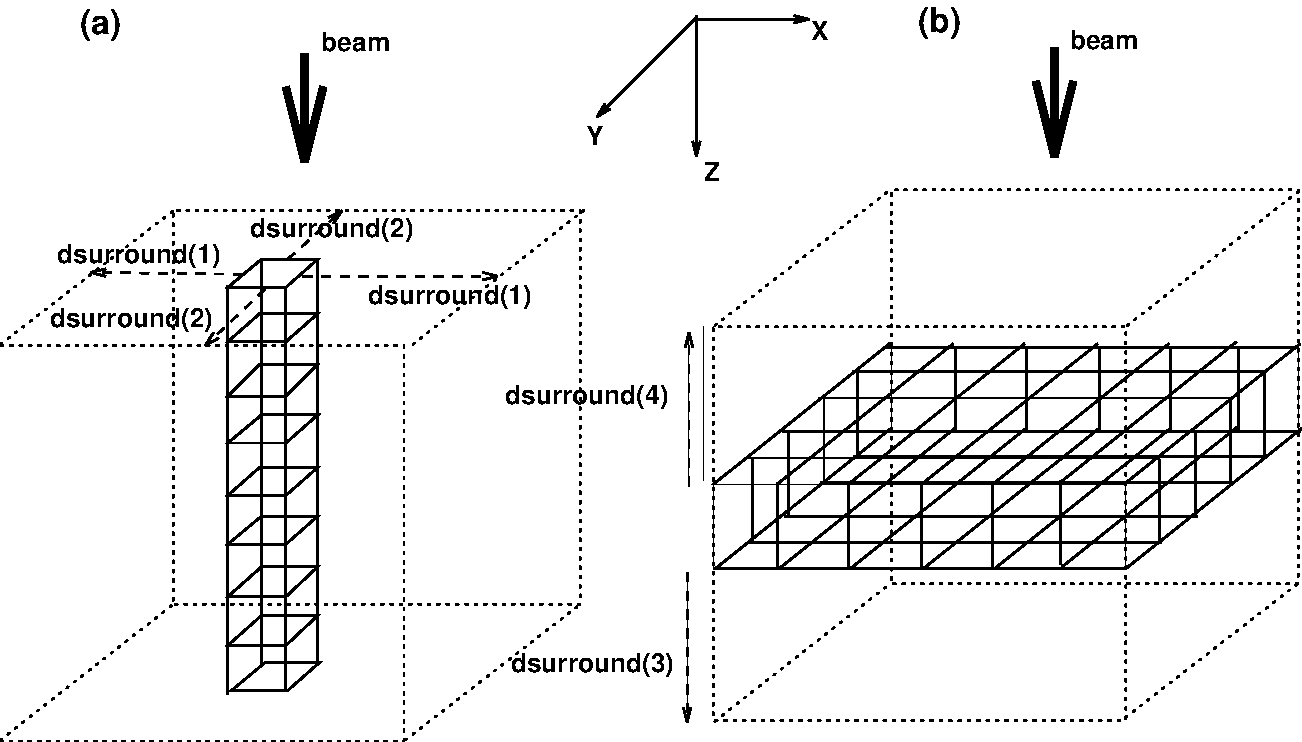
\includegraphics[height=8cm]{figures/dsurround_fig1}
\caption{Two examples of how {\tt dflag} and {\tt dsurround(1...4)} can be used
to
specify a small group of voxels within a larger phantom of the same medium.
In (a) voxels are only specified in a single column for scoring depth-dose,
while the rest of the phantom is defined using {\tt dsurround(1)} and
{\tt dsurround(2)} ({\tt dsurround(3)} and {\tt dsurround(4)} are 0 in this
particular example).  (b) shows voxels specified in a horizontal slice
for scoring the dose profile at a given z value.
In this latter example, the dimensions of the phantom below and above the
slice are defined by {\tt dsurround(3)} and {\tt dsurround(4)} respectively.
{\tt dsurround(1)} and {\tt dsurround(2)} are set to 0 in (b).}
\label{fig_dsurround}
\end{center}
\end{figure}

\lfoot[{{\sffamily \leftmark}}]{{\small Last edited $Date: 2013/09/24 14:49:18 $ }}

Table~\ref{dsurround_table} below shows the results of timing studies
performed using a beam of 10 MeV electrons and a beam
of 6 MV photons incident on a 59x59x10cm water phantom.  For
each beam, 4 cases were simulated: the entire volume filled with 1cm$^{3}$
voxels; 1cm$^{3}$ voxels specified in a column (1x1x10) down
the central (z) axis of the volume (similar to Figure~\ref{fig_dsurround}(a));
1cm$^{3}$ voxels specified in
a vertical slice (1x59x10) through the phantom in the y direction
at x=0; 1cm$^{3}$ voxels specified in a horizontal slice
(59x59x1) through the
phantom at z=2.5cm ($\sim$d$_{max}$)
(similar to Figure~\ref{fig_dsurround}(b)).  In
all cases, simulations were run with and without range rejection.

\begin{table}[htbp]
\caption{Timing results for circular beams of 10 MeV electrons and 6 MV
photons incident on a water phantom.
In all cases, the phantom size is the same (59x59x10 cm$^3$), but the
1x1x1cm$^3$ voxels take up differing parts of the volume (see text).}
\label{dsurround_table}
\begin{tabular}{|p{3cm}|p{3cm}|p{4cm}|p{4cm}|}
\hline
source & number of voxel regions (all 1 cm$^3$) & \multicolumn{2}{|c|}{CPU time (hrs)}\\
\cline{3-4}
       &             & range rejection off & range rejection on \\
\hline
\hline
10 MeV electrons & 59x59x10~~~~~~~ uniform & 0.576 & 0.559 ({\tt ESAVE}=5MeV)\\
\cline{2-4}
(r=10 cm, & 1x1x10 central axis & 0.181 & 0.100 \\
\cline{2-4}
1x10$^{6}$ histories) & 1x59x10 vertical plane & 0.208 & 0.141\\
\cline{2-4}
 & 59x59x1 horizontal plane & 0.345 & 0.300\\
\hline
\hline
6 MV photons & 59x59x10 & 1.623 & 1.525 ({\tt ESAVE}=3MeV)\\
\cline{2-4}
(r=10 cm, & 1x1x10 & 0.785 & 0.479\\
\cline{2-4}
30x10$^{6}$ histories) & 1x59x10 & 0.824 & 0.551\\
\cline{2-4}
 & 59x59x1 & 0.969 & 0.711\\
\hline
\end{tabular}
\end{table}

The table shows that if a depth-dose curve is all that is required, then
specifying voxels only in a 1x1x10cm column can decrease
simulation time by a factor of 5.5 for the electron beam and
a factor of 3 for the photon beam.
In general, the CPU time increases
as the number of voxels specified increases, but orientation of the volume
in which voxels are specified plays a role as well.
The 59x59x1cm horizontal slice
is, relatively, the least efficient use of {\tt dsurround} (saving a factor of
$\sim$2 in CPU time) due to the fact that it has more voxels than the
central-axis phantom and the vertical slice phantom but also due to the fact
that most of the primary and secondary particles from the beam have to be
transported across the
horizontal voxel boundaries defining the slice.  Finally, note that range
rejection is
more efficient when using {\tt dsurround} with a smaller number of
voxels:
turning range rejection on decreases the
simulation time for the case where voxels are only specified in a 1x1x10cm
column by a factor of almost 2, while
its effect on the simulation time when the entire phantom is divided into
voxels is negligible.

Note that this option allows electrons to take much bigger steps in the
{\tt dsurround} regions and this can cause some small inaccuracies unless
the default EGSnrc transport parameters are used.

\section{Pegsless mode}
\indexm{pegsless mode}

As of 2013, DOSXYZnrc can be run independent of the pegs4 cross section data file.  Photon
cross sections had been calculated on the fly since 2006, so the move towards a completely pegsless
version of EGSnrc-based user codes was a logical one.

When running in pegsless mode, all media used in the simulation must be defined
in the {\tt .egsinp} file, between the delimiters, {\tt :start media definition:} and {\tt :stop media definition:}.
{\tt .egsinp} file.  Here, the user has the option of specifying the name of a material data file, containing
\indexm{pegsless mode!material data file}
the compositions, bulk densities, etc, of the media and/or defining media parameters directly in the {\tt .egsinp} file.  The latter method is useful for defining media not included in the material data file or for overriding parameters
in the material data file.  The user also specifies the particle energy limits for cross section calculation:
\indexm{pegsless mode!AE}\indexm{pegsless mode!UE}\indexm{pegsless mode!AP}\indexm{pegsless mode!UP}
{\tt AE} and
{\tt UE} for electrons, {\tt AP} and {\tt UP} for photons.   For more information about the inputs
between the {\tt :start media definition:} and {\tt :stop media definition:} delimiters, including defaults, you are
urged to refer to the BEAMnrc Users Manual\cite{Ro09}.

Pegsless mode is accessible through the DOSXYZnrc GUI by selecting ``Change PEGS4 file'' from the ``File'' menu and
then opting to ``Go PEGSless'' instead of selecting a PEGS4 file.  Once you have done this, a ``Define Media'' button
at the bottom of the main input window becomes active.  Pushing this button will open up a sub-window through
which you have access to the inputs between {\tt :start media definition:} and {\tt :stop media definition:} in
the {\tt .egsinp} file.

\indexm{pegsless mode!running in}
DOSXYZnrc can be run interactively in pegless mode using the command line input:
\begin{verbatim}
dosxyznrc -i inputfile
\end{verbatim}
where {\tt inputfile} is the name of the input file (with no
{\tt .egsinp} extension).

Pegsless batch runs use the command line syntax:
\begin{verbatim}
exb dosxyznrc inputfile pegsless [short|medium|long] [batch=batch_system] [p=N]
\end{verbatim}
This is identical to the syntax of a run with pegs data (see Section~\ref{candrsect} above) but
with the word {\tt pegsless} in place of the name of the pegs data file.

\indexm{pegsless mode!.mederr file}
On termination, pegsless runs output a file, {\tt inputfile.mederr}, containing information about where
the specifications for each medium in the simulation have been read ({\it i.e.} from the material data
file or directly from {\tt inputfile.egsinp}) and various warning messages related to inputs that have
been left blank and have been set to their default values.  The media compositions and settings for other
parameters necessary for calculating cross sections are output to {\tt inputfile.egslst} and
{\tt inputfile.egslog} (for batch runs).

\section{CT Based Phantoms/{\tt ctcreate}}
\indexm{ctcreate}
\indexm{CT!phantoms}

The CT phantom option of DOSXYZnrc allows calculation of dose distributions in
phantoms that are derived from CT data sets. This
allows simulations in realistic anthropomorphic
phantoms. (Please note that the previous sentence does not use the
word patient.)  The creation of CT phantoms from CT data is performed
using the stand-alone code, {\tt ctcreate}.

\indexm{Pinnacle CT}
\indexm{AAPM CT}
\indexm{CT!format!AAPM}
\indexm{CT!format!CADPLAN}
\indexm{CT!format!Pinnacle}
\indexm{CT!format!DICOM}
\indexm{CADPLAN CT}
At this point in time, {\tt ctcreate} supports CT data in DICOM
format (with some restrictions, see below), ADAC
Pinnacle format, and CADPLAN format.
A tool for converting the AAPM CT format into
Pinnacle format is also available.

The process by which CT phantoms are created by {\tt ctcreate}
\indexm{ctcreate}
are outlined here and described in detail in the following sections.

\begin{enumerate}
\item Read in the format of the CT data
\item Read in the CT header parameters (binary or ASCII).
\item Read in the binary CT data.
\item Choose a subset of the CT data set (if desired).
\item Resample the CT data to correspond to volume elements that dose
will be scored in.
\item Convert the CT data to materials and densities for each voxel.
\item Transfer the data via a file to be input to DOSXYZnrc.
\end{enumerate}

\indexm{.egsphant}
\indexm{files!.egsphant}
The relevant CT phantom information
is written into the file, {\tt *.egsphant} (prefix is the same as the
original CT data set name).  A flowchart for the CT phantom code, showing
how it relates to DOSXYZnrc is shown in figure~\ref{fig_ct01}.

Nearly all of the CT phantom functionality takes place outside of
{\tt ctcreate} proper in subroutines.  This
\indexm{ctcreate}
modularity allows for easy changes in the code by ambitious users (for example subroutines for
other CT file formats).  Specifically, this is to provide the user with the
means of reading
their own CT file formats and writing their own dose distribution files
 without rewriting large chunks of
{\tt ctcreate.mortran} and {\tt dosxyznrc.mortran}. This can be accomplished
by creating their
own versions of the subroutines {\tt ReadCT} in {\tt ctcreate.mortran} and
{\tt write\_dose} in {\tt dosxyznrc.mortran}. The
specifications as to what
is required of these subroutines can be found in the codes themselves and
in section~\ref{spec_ReadCT} of this document.

\indexm{CT!coordinate system}
Note that the input CT data set defines the coordinate system for the
calculation, which may be different from the coordinate system of the
accelerator simulation (using BEAM).  For example, for Pinnacle CT
\indexm{Pinnacle CT}
data sets, the Z-axis is typically down the centre of the patient whereas in
the accelerator simulation the Z-axis is the beam's central axis.  This
causes no problems, but must be kept in mind.

\begin{figure}[htbp]
\begin{center}
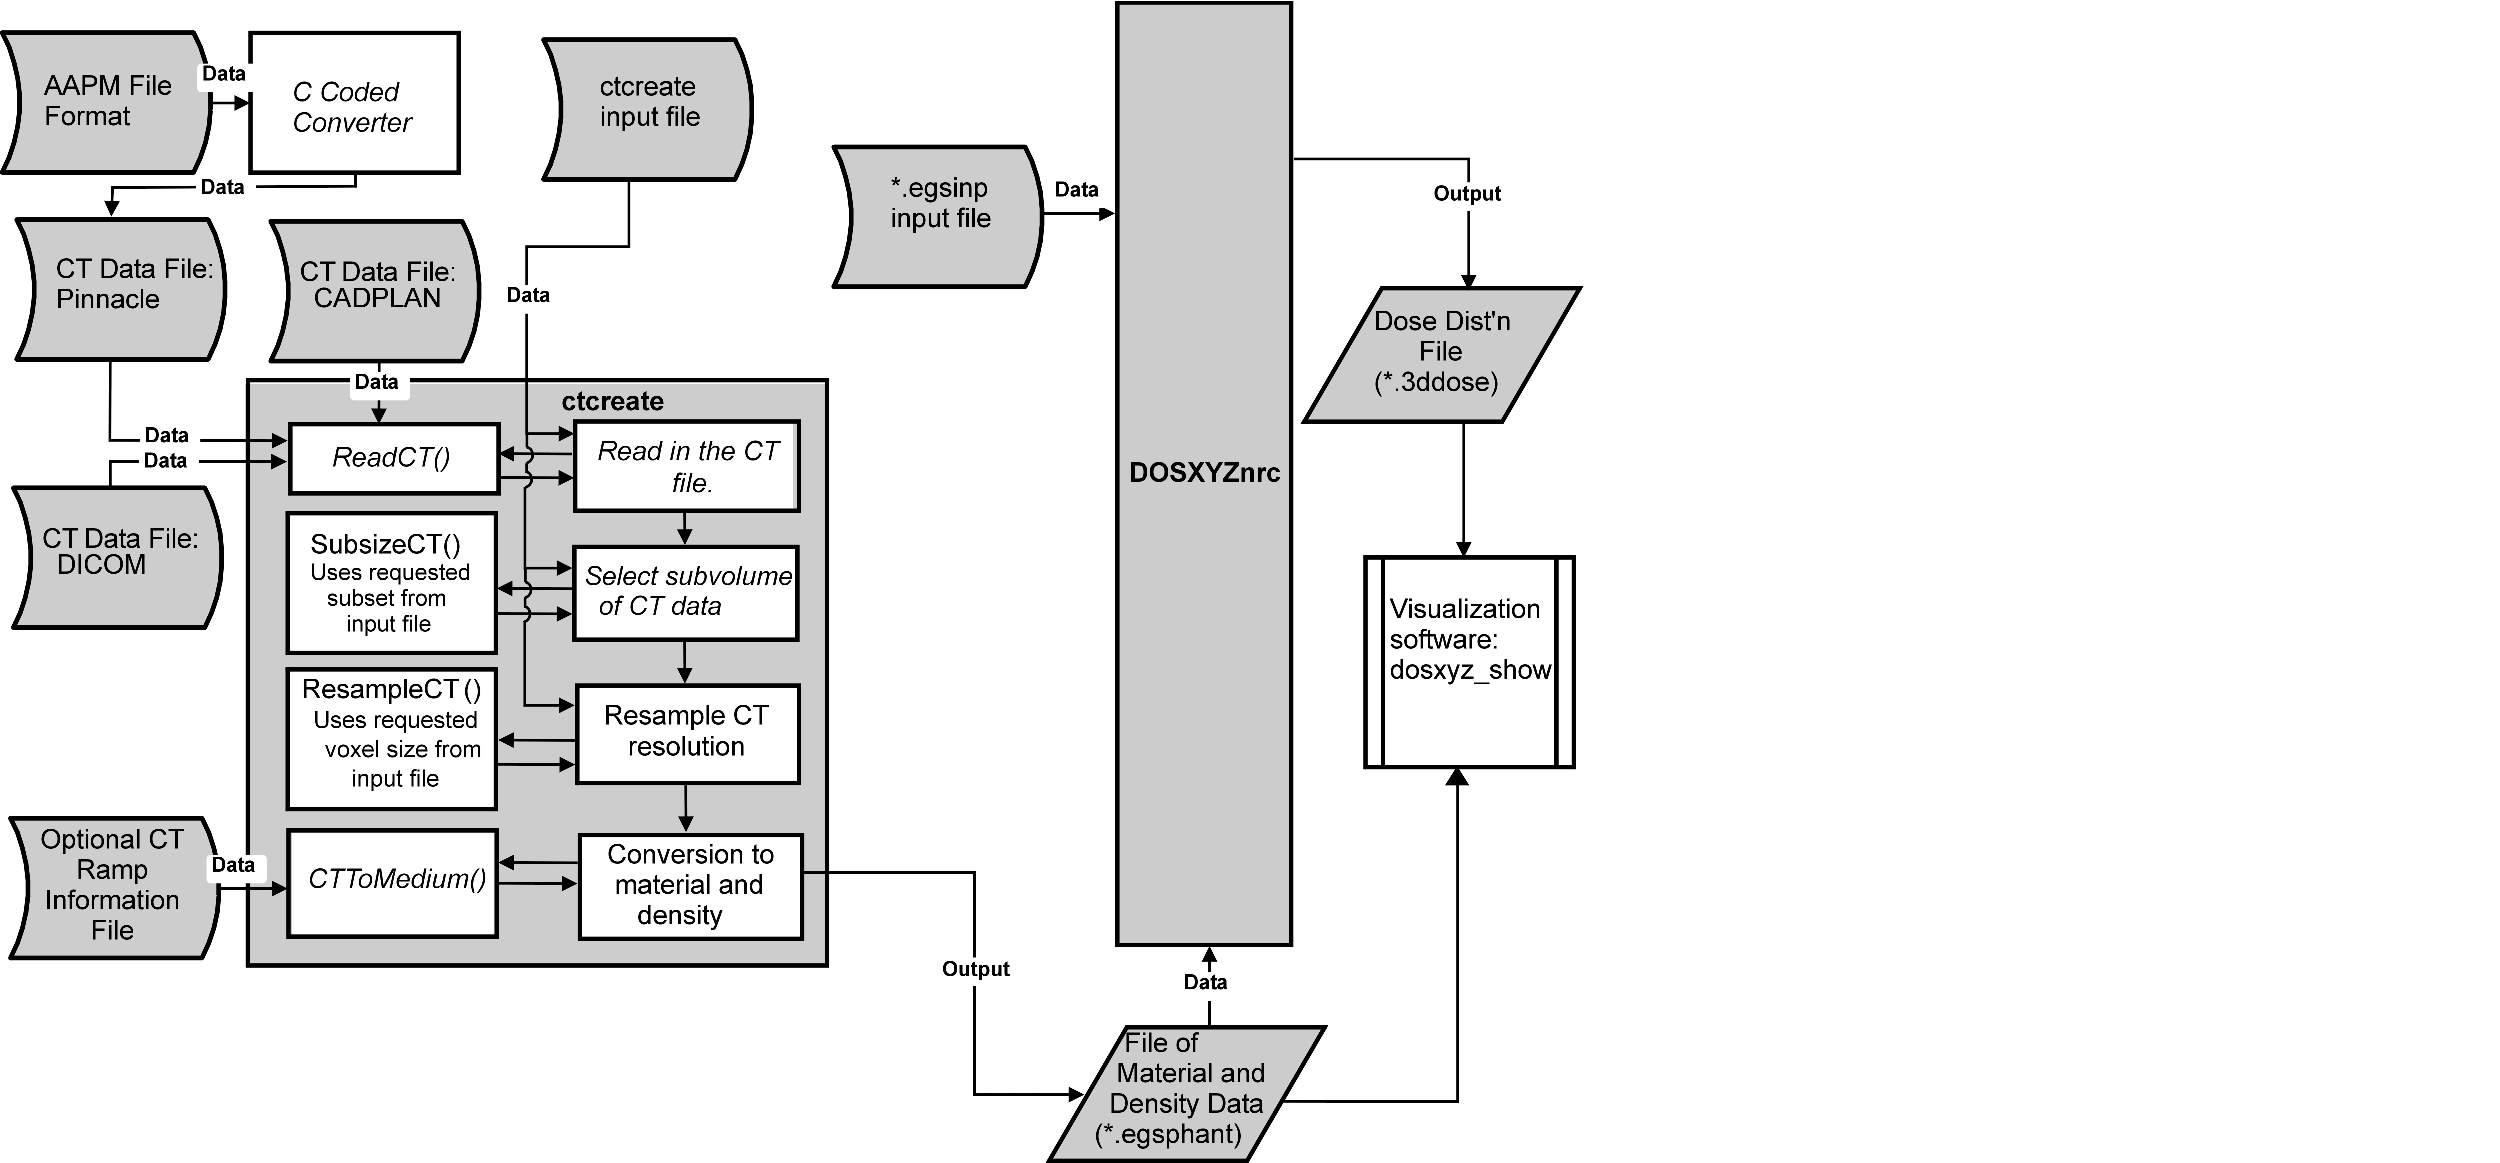
\includegraphics[height=12cm]{figures/ct_fig1}
\caption{A flowchart for use of CT data with  {\tt ctcreate} and DOSXYZnrc. }
\label{fig_ct01}
\end{center}
\end{figure}

\subsection{Using the CT Phantom Option in DOSXYZnrc}

\indexm{CT!option}
\indexm{nmed}
The CT phantom option is used by setting the number of materials,
{\tt nmed} in record 2 of the DOSXYZnrc input file, to zero. This will cause the
program to execute differently than when {\tt nmed} is $>$ 0, and, instead
of geometry, material and density data for the phantom being input explicitly
in the DOSXYZnrc input file,
DOSXYZnrc reads these data from a CT phantom file which has
been created using {\tt ctcreate}.  The input for the
CT and non-CT modes of DOSXYZnrc
are common again after this input (see section~\ref{DOSXYZ_input},
page~\pageref{DOSXYZ_input}).

In short, the input file for DOSXYZnrc is very different if the CT
option is being used.  From section~\ref{DOSXYZ_input} it can be seen
that in CT mode, input records 3-9 in non-CT mode are replaced by
records 3-5, which specify the name of the file containing the CT phantom
data, the transport parameters, and some output parameters.

\subsection{Using {\tt ctcreate}}

\indexm{ctcreate}
\indexm{.egsphant}
\indexm{files!.egsphant}
This section covers the input parameters that {\tt ctcreate} requires
to create a {\tt *.egsphant} CT phantom file that can then be read in and
used by DOSXYZnrc.

It is fairly simple to obtain a
CT phantom from the CT data set since all the required material and geometry
information is contained in the data set.
The additional information that the user is required to provide
are the CT data format, the name of the file containing either the header
info (Pinnacle) or containing the names of the actual CT data files (CADPLAN
and DICOM),
voxel dimensions for the phantom. The user can also select a subset of the full
CT data and specify their own CT ramp (ie function for converting
\indexm{CT!ramp}
CT data to the densities and materials required for the DOSXYZnrc phantom).  Input
of a custom CT ramp is highly recommended.

The following are the input parameters for {\tt ctcreate}.  This description
is found at the beginning of the {\tt ctcreate.mortran} code.
\indexm{ctcreate!input parameters}
\begin{small}
\input{inputs/ctcreate.inp}
\end{small}
\indexm{running ctcreate}

Parameters may be input interactively, by typing:

{\tt ctcreate}

and responding to the prompts;  or stored in an input file
and {\tt ctcreate} run with the input file by typing:

{\tt ctcreate inputfilename}

{\tt ctcreate} input parameters are described in more detail in the subsections below.

\subsubsection{{\tt ctformat}}
\indexm{CT!format}
The first input required by {\tt ctcreate} is the format of the
CT data.  Currently, {\tt ctcreate} supports {\tt Pinnacle}, {\tt
CADPLAN} and {\tt DICOM} formats.
If the data is in AAPM format, then it can be converted to Pinnacle format
using the code
{\tt \$OMEGA\_HOME/progs/ctcreate/CT/AAPM/aapm2pinnacle}
\indexm{aapm2pinnacle}
\indexm{AAPM format}
\indexm{Pinnacle format}
\indexm{CADPLAN format}

\subsubsection{{\tt CTFilename}}
\indexm{CT!data file}
\indexm{CTFilename}
{\tt CTFilename} is the full name of a file, the contents of which depend
on the CT data format:
\begin {description}
\item [Pinnacle format]
\indexm{Pinnacle CT}
{\tt CTFilename} is the full name of the header file of the CT data set
(including the {\tt .header} extension).
The code
will read in all the information that it requires from this file before
moving on to read in the entire binary data file (which has an assumed
extension {\tt .img} and the same prefix as the header file).
  %A sample Pinnacle header file is shown in the next section of this document.
\item [CADPLAN and DICOM formats]
\indexm{CADPLAN CT}
\indexm{DICOM CT}
{\tt CTFilename} is the full name ({\it i.e.} including directory path)
of a file containing the full names of the
individual CT data files (1 file/image slice).  The file names MUST appear
in order of increasing Z position of the slice.
\end{description}

\indexm{.egsphant}
\indexm{files!.egsphant}
On output, the CT phantom will be named:\\
{\tt CTFilename(minus .header extension if using Pinnacle format).egsphant}\\

\subsubsection{{\tt xctsubmin,xctsubmax,yctsubmin,yctsubmax,zctsubmin,zctsubmax}}
\indexm{CT!sub-volume}
\indexm{xctsubmin}
{\tt xctsubmin},{\tt xctsubmax}, {\tt yctsubmin}, {\tt yctsubmax},
{\tt zctsubmin},
and {\tt zctsubmax} are used to create six planes which describe a cube.
The subsection of the original CT data contained in this cube will
be used to create the CT phantom. In this
manner only the portion of interest in the original CT data is used in
the simulation.  This allows the particle simulation
to be performed at a higher resolution than if the calculation used the
entire CT volume, and allows the user to trim some of the air that surrounds
a typical CT image from consideration in the phantom.  Note that if the
sub-volume selected by the user does not fit on an integer number of voxels
from the original CT data, then the sub-volume will automatically be expanded
until it does so.

\subsubsection{{\tt xyz\_xthickness,xyz\_ythickness,xyz\_zthickness}}
\indexm{CT!phantom voxels}
\indexm{voxel size}
\indexm{xyz\_xthickness}
The third line of the input to {\tt ctcreate} is the
spatial resolution that the user requires for the simulation.
{\tt xyz\_xthickness}, {\tt xyz\_ythickness}, {\tt xyz\_zthickness}
are the 3 dimensions of the voxels to be used in the CT phantom.
The maximum voxel dimension in a given direction is
the distance between the planes delimiting the subset of the CT data
to be used in that direction (see previous section).
The minimum voxel dimension in a direction is the distance between
the planes delimiting the subset of CT data in that direction divided
by the maximum number of voxels allowed in that direction (set at
compilation).
{\tt ctcreate} will alert the user when dimensions less than the minimum
or greater than the maximum are input.  Note that, if necessary, the voxel
dimensions will always be increased to fit an integer number of DOSXYZnrc
voxels on the CT sub-volume selected by the user.

\subsubsection{{\tt num\_material}, {\tt material\_ct\_lower\_bound}, and other CT ramp inputs}
\indexm{CT!ramp}

{\tt num\_material} is the
number of materials in the ramp function used
to convert CT number in each voxel to material and density.
If this is set to zero then a
default CT ramp is used in the conversion. The default ramp
is shown in Figure~\ref{fig_ct02} and in the sample input file given in the next section.
{\tt material\_ct\_lower\_bound} defines the lowest CT number of the first ramp
({\it i.e.} the lowest CT number for material  1).  If the default ramp is used, then {\tt material\_ct\_lower\_bound} defaults
to -1024, which is typically the minimum CT number for air in DICOM format data.

If {\tt num\_material} $>$0 then
the CT ramp is read from
the input file.  For each medium in the ramp, there are
two lines of input. \indexm{CT!ramp}
The first of these lines is the name of the material
({\tt material\_name}) which must be identical to a material in the
{\tt PEGS4} material data file being used in the DOSXYZnrc simulation.
The second line specifies the maximum CT number for the medium, {\tt material\_ct\_upper\_bound},
the minimum density of the medium, {\tt material\_density\_lower\_bound}, and the maximum
density of the medium,
{\tt material\_density\_upper\_bound}. Note that the ramp is assumed to be continuous
in CT number.  Thus, for material {\tt n}, {\tt material\_density\_lower\_bound(n)} corresponds
to a CT number of {\tt material\_ct\_upper\_bound(n-1)} (or the overall
minimum CT no. of the ramp, {\tt material\_ct\_lower\_bound}, if
{\tt n}=1), and {\tt material\_density\_upper\_bound(n)} corresponds to
{\tt material\_ct\_upper\_bound(n)}.
Also note that the ramp must be input in order of
increasing {\tt material\_ct\_upper\_bound}.

The CT ramp is then used to determine the medium and density in each voxel of the CT data.
\indexm{CT!ramp}
If a voxel's CT number is $\leq$ {\tt material\_ct\_upper\_bound(n)} and
$>$ \\
{\tt material\_ct\_upper\_bound(n-1)} (or {\tt material\_ct\_lower\_bound} if
{\tt n}=1)
then it is assigned medium {\tt n}. The density is then calculated using a linear
interpolation between the medium's density limits:
\begin{align}
{\tt r}&{\tt hor}_{i,j,k} = {\tt material\_density\_lower\_bound(n)} \nonumber \\
             &+\left(\frac{{\tt material\_density\_upper\_bound(n)}-
 {\tt material\_density\_lower\_bound(n)}}
{{\tt material\_ct\_upper\_bound(n)}-
 {\tt material\_ct\_upper\_bound(n-1)}}\right)        \\
        &*({\tt CT}_{i,j,k}-{\tt material\_ct\_upper\_bound(n-1)}) \nonumber
\end{align}

The default ramp is shown in Figure~\ref{fig_ct02}. This is a modified version of
\indexm{CT!ramp}
a CT ramp given in Kawrakow et al\cite{Ka96a}.  Note that this ramp has been
optimized for typical DICOM format data, where the lowest CT number for air
{\tt material\_ct\_lower\_bound} is -1024.

If the CT number in a voxel is less than {\tt material\_ct\_lower\_bound} then
the medium in that voxel is set to vacuum with density zero.
Those voxels with CT numbers above the
last material's upper CT number ({\tt material\_ct\_upper\_bound(num\_material)})
will have the density set to the maximum
density for the last material.

\begin{figure}[H]
\begin{center}
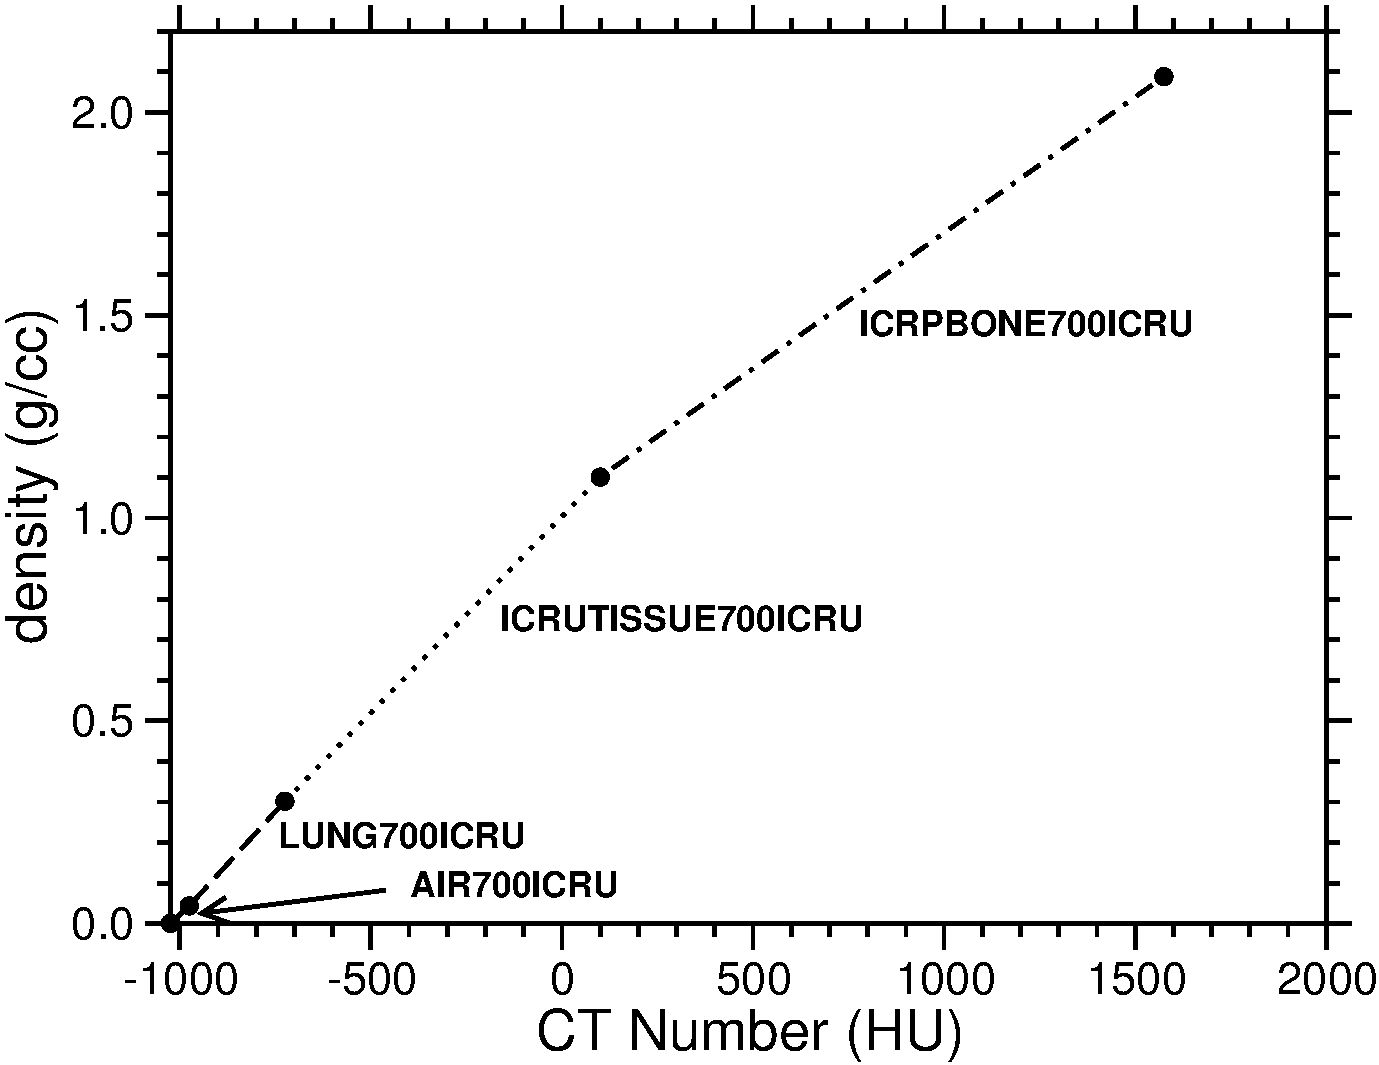
\includegraphics[width=10.5cm]{figures/CTramp}
\caption{The default ramp for converting CT values to material and
density in {\tt ctcreate} modified from Kawrakow et al\cite{Ka96a}.}
\label{fig_ct02}
\end{center}
\end{figure}
\indexm{CT!ramp}

The default CT ramp may be suitable for displaying a {\tt .egsphant} file
using {\tt dosxyz\_show}\cite{Ka98} and for example calculations.  However,
we strongly recommend that you explicitly enter your own CT ramp function
for more detailed simulations, since the CT ramp is
dependent upon the imager and the data acquisition method.

\subsection{Sample {\tt ctcreate} CT Phantom Input File}
\indexm{ctcreate!sample input}
Table~\ref{ctinpex} shows an example {\tt ctcreate} input file, and
a sample DOSXYZnrc input file (excluding EGSnrc inputs)
which uses the CT phantom data from {\tt ctcreate}.

\vspace*{-0.5cm}
\begin{table}[htbp]
%\begin{tabular}{|p{8cm}p{7.7cm}|}
\caption{Sample input files for {\tt ctcreate} and DOSXYZnrc}
\begin{tabular}{|p{7cm}p{8.7cm}|}
\hline
\bf{Input Parameter} & \bf{Description of input fields.} \\
\multicolumn{2}{|c|}{\bf for {\tt ctcreate}      } \\
{\tt DICOM} & CT data is in DICOM format \\
{\tt CTfname} & in DICOM format, this is the name of a file containing the names of the individual image slices (in order
of increasing Z).
\\
%\hline
{\tt -17.64,17.64,-17.64,17.64,-0.7,4.3}
&
The subvolume of the CT data set
that is to be used for the phantom.
\\
%\hline
{\tt 1.0, 1.0, 1.0 }
&
The phantom voxel size.
\\
%\hline
{\tt 4, -1024}
&
{\tt num\_material}, {\tt material\_ct\_lower\_bound}.
If {\tt num\_material}=0
the default ramp will be used.
The default values are
listed explicitly in this example.
\\
%\hline
{\tt AIR700ICRU }
&
The material\_name for the first material.
\\
%\hline
{\tt -974,0.001,0.044}
&
CT ramp parameters for the first material:\\
&{\tt  material\_ct\_upper\_bound}, \\
&{\tt material\_density\_lower\_bound},\\
&{\tt material\_density\_upper\_bound}
\\
%\hline
{\tt LUNG700ICRU }
&
The material name for the second material.
\\
%\hline
{\tt -724,0.044,0.302}
&
The ramp parameters for the second material. \\
%\hline
{\tt ICRUTISSUE700ICRU} & The material name for the third material.
\\
%\hline
{\tt 101,0.302,1.101} & The ramp parameters for the third material.
\\
%\hline
{\tt ICRPBONE700ICRU} & The material name for the fourth material.
\\
%\hline
{\tt 1976,1.101,2.088} & The ramp parameters for the fourth material.
\\
\hline
\multicolumn{2}{|c|}{\bf for DOSXYZnrc} \\
%\hline
{\tt Sample CT Input File } & Title of the simulation and phantom. \\
%\hline
0 & {\tt NMED } - If this is zero the code switches to CT\_Phantom mode. \\
%\hline
{\tt CTfname.egsphant} & The name of the CT phantom file.\\
{\tt 0.7,0.01,5.0} & {\tt ECUTIN}, {\tt PCUTIN}, {\tt SMAX} (dummy inputs)\\
{\tt 1,0,1} & {\tt zeroairdose}, {\tt doseprint} and {\tt MAX20} \\
%\hline
{\tt -1,0,-1.25,1.25,-2.25,2.25,90.0,} & The source description record.
At this point the \\
{\tt 90.0,0.0} &CT phantom input meets up with the manual\\
& phantom inputs.
\\
%\hline
{\tt 0}
&
monoenergetic particle spectrum.
\\
%\hline
{\tt 20.0 }
&
particle energy.
\\
%\hline
{\tt 100,0,500.,7,3,100.,0,0,0,1,5.0,} & Monte Carlo information (note range rejection \\
\hspace*{1cm}{\tt 0,0,0,0}&below 5MeV).  \\
%\hline
\hline
\end{tabular}
\label{ctinpex}
\end{table}

\subsection{Location of {\tt ctcreate} and How to Compile It}
\label{comp_ctcreate}
{\tt ctcreate.mortran} and related files
(see section~\ref{filesect} for a complete list)
\indexm{ctcreate!installation}
reside in the subdirectory {\tt \$OMEGA\_HOME/progs/ctcreate}.
Normally, it is compiled as part of the OMEGA/BEAM installation
(see the BEAMnrc Manual\cite{Ro04a} for installation instructions), however
it can be compiled separately by going into this directory and
typing {\tt make}.

\subsection{{\tt ReadCT()} Subroutines}
\label{spec_ReadCT}
\indexm{ReadCT}
\indexm{CT!format!AAPM}
\indexm{CT!format!CADPLAN}
\indexm{CT!format!DICOM}
\indexm{CT!format!Pinnacle}
{\tt ReadCT} is the most important subroutine in {\tt ctcreate}.  It handles
the reading in of header information and binary CT data.  Currently, there
are three {\tt ReadCT} subroutines within {\tt ctcreate}, one for each of the CT formats
supported: {\tt ReadCT\_Pinnacle} for Pinnacle, {\tt ReadCT\_CADPLAN}
for CADPLAN data and {\tt ReadCT\_DICOM} for DICOM data.

\subsubsection{{\tt ReadCT\_Pinnacle}}
\indexm{ReadCT\_Pinnacle}
\indexm{CT!format!Pinnacle}

{\tt ReadCT\_Pinnacle} is contained
within the {\tt ctcreate.mortran} file and calls
other subroutines and functions in this file:
\begin{description}
\indexm{ReadReal}
\indexm{ReadInt}
\indexm{read\_ct\_data}
\indexm{swap\_bytes}
\item[{\tt ReadReal}] Reads real values from the image header ({\tt .header}) file.
\item[{\tt ReadInt}] Reads integer values from the header file.
\item[{\tt read\_ct\_data}] Reads binary CT data from the image ({\tt .img})
file.
\indexm{swapping bytes}
\item[{\tt swap\_bytes}] Swaps bytes of CT data if there is a
byte order mismatch between the data and the machine you are using.
\end{description}

Note that in Pinnacle format CT numbers are $>$ 0.  Thus, the default CT ramp
in {\tt ctcreate} cannot be used to convert CT numbers to media and densities.
The example {\tt ctcreate} inputfile, {\tt \$OMEGA\_HOME/progs/ctcreate/ctcreate\_examples/CT\_create.inp}
(used in Lab VI in the BEAMnrc Workshop), is used to convert Pinnacle format data and
contains a custom CT ramp which is just the default ramp shifted up by 1025 HU.

\subsubsection{{\tt ReadCT\_CADPLAN}}
\indexm{ReadCT\_CADPLAN}
\indexm{CT!format!CADPLAN}
{\tt ReadCT\_CADPLAN} is also contained
within the {\tt ctcreate.mortran} file.
Unlike {\tt ReadCT\_Pinnacle}, {\tt ReadCT\_CADPLAN} is a self-contained subroutine.
Byte swapping is not required since single bytes are read at a time.


\subsubsection{{\tt ReadCT\_DICOM.c}}
\indexm{CT!format!DICOM}
\indexm{ReadCT\_DICOM}
{\tt ReadCT\_DICOM.c} is a separate C routine whose object file is linked
to {\tt ctcreate} at compile time.  {\tt ReadCT\_DICOM.c} is automatically
compiled when you {\tt make} ctcreate.
{\tt ReadCT\_DICOM.c} requires the C header file {\tt tags\_ct.h}, which
defines hexadecimal tags, or labels, for the DICOM data.  These tags
are defined in the DICOM standard, and if the user modifies
{\tt ReadCT\_DICOM.c} to deal with additional tags, then these can
be added to the {\tt tags\_ct.h} file.
Currently,
{\tt ReadCT\_DICOM} assumes
\indexm{little endian byte order}
\indexm{big endian byte order}
the DICOM data has been collected on a machine with little endian byte order
(ie compatible with Linux), however, if the data was collected on a machine
with big endian byte order, you must go into {\tt ReadCT\_DICOM.c} and
change the line:
\indexm{DICOM\_ENDIAN}
\begin{verbatim}
#define DICOM_ENDIAN 1
\end{verbatim}
to:
\begin{verbatim}
#define DICOM_ENDIAN 0
\end{verbatim}
and recompile {\tt ctcreate}.  The endianness of the machine you
are running {\tt ctcreate} on is automatically detected by
{\tt ReadCT\_DICOM} and then bytes are swapped if necessary.

The DICOM format is known to vary from imager to imager and institute
to institute.  Thus, we cannot guarantee that {\tt ReadCT\_DICOM} will
work with your images without modification.  As a minimum,
the current version of {\tt ReadCT\_DICOM} requires the following
information in the image (slice) header(s):
\begin{enumerate}
\item Number of rows (data tag {\tt 0x00280010}).  This defines the number of voxels in the X-direction.
\item Number of columns (data tag {\tt 0x00280011}). This defines the number of voxels in the Y-direction.
\item Pixel spacing (data tag {\tt 0x00280030}).  Defines the X- and Y-dimensions of the voxels.
\item Image position (data tag {\tt 0x00200032}). Defines the (X,Y,Z) of the centre of the first voxel.  The position
of the first slice (slice with lowest Z) is used to determine the X-, Y- and
Z-offset (starting position) of the CT data, and the Z-positions of the first two slices are used
to established voxel Z-dimension ({\it i.e.} slice thickness).
The Z-positions of slices as read from the header are also used to
sort slices in order of increasing Z, in case the user has not already done so
in the file containing the slice names.
\item A pixel data tag ({\tt 0x7fe00010}) indicating the size of the data array in bytes.  This tag must appear last in the
header, immediately preceding the CT data itself.
\end{enumerate}

{\tt ReadCT\_DICOM} assumes slices are contiguous in Z.  Thus, once the Z-position of the first slice and slice thickness (Z-dimension of voxels) are
established, {\tt ReadCT\_DICOM} positions subsequent slices so that there are no gaps
or overlaps between them.  A warning message is output if the Z-position of
a slice determined by {\tt ReadCT\_DICOM} does not equal the Z-position
of the slice as read from the image position in its header.

We note that {\tt ReadCT\_DICOM.c} has limited flexibility in terms of slice
layout, and it has not been
tested on all possible variations of the DICOM format.  Therefore, if you
require more flexibility or are having trouble converting your DICOM files, you
are strongly urged to either modify {\tt ReadCT\_DICOM} or use your own
stand-alone routine for converting DICOM images to {\tt .egsphant} files.

\indexm{Nick Reynaert}
The initial version of {\tt ReadCT\_DICOM.c} was provided by Nick Reynaert at the University of Ghent.

\subsubsection{Generic {\tt ReadCT}}
\indexm{ReadCT!Generic}

Essentially, {\tt ReadCT} is the subroutine or stand-alone
code which the user will have to
\indexm{ReadCT specs}
customize or program from scratch to deal with any CT format not currently
handled.  The structure and number of subroutines within {\tt ReadCT} is
largely a matter of the programmer's taste.  However, if {\tt ReadCT} is
to be included in {\tt ctcreate} (or linked as an object file when compiling
{\tt ctcreate}), it must
pass certain essential data back to {\tt ctcreate}.   An example call to
a generic {\tt ReadCT} routine is:

\noindent {\tt Subroutine ReadCT(fname,asize,ctdata,offset,vsize,error)}

\noindent where {\tt fname} is a character string containing the name of the
particular CT data set.  The essential CT data returned to {\tt
ctcreate} are:
\begin {description}
\item [{\tt asize(3)}]  An array returning the number of CT voxels in the
                     x,y,z directions.
\item [{\tt vsize(3)}]  An array returning the dimensions of the CT voxels

\item [{\tt offset(3)}] An array returning the lower bounds of the CT data
                      in the x,y,z directions in cm.
\item [{\tt ctdata(\$CTIMAX,\$CTJMAX,\$CTKMAX)}] A 3-D integer array
           returning the CT data (Hounsfield numbers).  In {\tt ctdata},
    {\tt x}$\rightarrow${\tt i},
    {\tt y}$\rightarrow${\tt j},
    {\tt z}$\rightarrow$ {\tt k}, so that {\tt ctdata(i,j,k)} is
    equal to the Hounsfield number in the voxel with lower bounds
    {\tt x=offset(1)+(i-1)*vsize(1)}, {\tt y=offset(2) +} {\tt (j-1)*vsize(2)},
    {\tt z=offset(3)+} {\tt (k-1)*vsize(3)} and
    upper bounds {\tt x=offset(1)+} {\tt i*vsize(1)},
    {\tt y=offset(2)+} {\tt j*vsize(2)}, {\tt z=offset(3)+} {\tt k*vsize(3)}
\item [{\tt error}] Returns the error status of the CT read operation.
                    Currently not used.
\end {description}

\subsection{Description of the {\tt *.egsphant} File}
\label{egsphantsect}
\indexm{.egsphant}
\indexm{files!*.egsphant}
The {\tt *.egsphant} file output by {\tt ctcreate} or by DOSXYZnrc itself
is an ASCII file
containing the following information necessary for DOSXYZnrc to simulate
the CT phantom and for the display program, {\tt dosxyz\_show}\cite{Ka98},
to display the density information:
\begin{enumerate}
\item The number of media in the phantom
\item The names of the media
\item The {\tt ESTEPE} value for each medium (now a dummy input)
\item The number of voxels in the X, Y and Z directions
\item A list of the voxel boundaries in the X direction
\item A list of the voxel boundaries in the Y direction
\item A list of the voxel boundaries in the Z direction
\item For each Z slice, an X-Y array containing the medium
      number in each voxel
\item For each slice in the Z direction, an X-Y array containing the densities
      in each voxel
\end{enumerate}
\vspace*{-0.3cm}
In addition to passing the necessary medium information to DOSXYZnrc, the X-Y
arrays of medium numbers (item 8 above) provide a rough slice-by-slice
view of the CT phantom.  A sample X-Y array of medium numbers from one slice of a CT phantom derived
from a lung image is shown below (hold at a distance, and raw data on
screen is easier to see):

\input{inputs/mednoarray.inp}

The user can use these slice-by-slice views to
determine whether the CT data is being read in correctly by {\tt ReadCT}
or to verify that the sub-volume of the original CT data selected
includes the physiology of interest.

\subsection{Files and Macros for implementation.}
Below is a short description of the files and macros required to compile
and run {\tt ctcreate} and DOSXYZnrc with CT phantoms.
\indexm{ctcreate!files and macros}

\begin{description}
\item[{\tt dosxyznrc\_user\_macros.mortran}]
{\tt ctcreate} uses the version stored in\\
{\tt \$HEN\_HOUSE/user\_codes/dosxyznrc}
to obtain {\$IMAX}, {\$JMAX} and {\$KMAX},
the maximum X, Y and Z dimensions of the CT phantom allowed in DOSXYZnrc.

\item[{\tt \$CTIMAX, \$CTJMAX, \$CTKMAX }]
Macros defining the maximum X, Y and Z dimensions of the CT data to be read in.
These macros are in {\tt ctcreate.mortran}

\item[{\tt lnblnk1.mortran}] {\tt MORTRAN} macro to provide the
FORTRAN {\tt lnblnk} function for Linux, rs6000 and HP9000 machines.
{\tt ctcreate} makes extensive use of this function and DOSXYZnrc uses it
in CT phantom mode.  It
is read from the {\tt \$HEN\_HOUSE/src} directory
\end{description}

\section{Known Bugs/Restrictions}

A restarted run that uses a phase space source with particle recycling will
not produce dose/uncertainty results identical to a single run with
the same total number of histories.  This is because the last particle
used before the restart may not have been recycled the full
{\tt NRCYCL} times, and restarting automatically skips to the next particle.
Results will agree within uncertainty, however.

It is recommended that when using the built-in parallel processing
functionality you do not restart parallel runs that use
a phase space source.  In this case, parallel jobs have lost track
of which chunks of the phase space source they were using in the
original run and the uncertainty analysis after recombining the
restarted runs will not take into account correlations due to reusing
chunks of the phase space source.

\section{Acknowledgments}

Charlie Ma was a major contributor to the DOSXYZ code and was the senior
author of the original DOSXYZ manual. Since he is not directly involved
with DOSXYZnrc, he is no longer an author of the manual, but his
contribution to the original code while he was at NRC still plays a
significant role in the current version.


A variety of people have contributed various pieces of code to the
DOSXYZnrc program.  We wish to thank: Julie Zachman of UW for providing
the aapm2pinnacle tool; Daryoush Sheikh-Bagheri for developing PAW
macros for displaying dose distributions and CT files; Geoff Zhang and
Daryoush again for extensive use of the code and drawing our attention
to bugs; Alex Bielajew for early work on the code; Marc Lauterbach and
Joerg Lehmann for initial coding to read CADPLAN CT data sets.
We also wish to thank Paul Reckwerdt for his work on the original code to
read Pinnacle CT data sets; Mark Holmes for his extensive work on reading
CT data and for coding the correlated sampling routines\cite{Ho99}; Brian
Geiser for the BTREE beam modeling method\cite{Ge95}.  \indexm{CADPLAN CT}

\begin{latexonly}
\section{References}
\end{latexonly}
\renewcommand{\rightmark}{References}
\indexm{references}
\typeout{****references start here}
\setlength{\baselineskip}{0.4cm}
\vspace*{-1cm}
\bibliography{../irs}
\bibliographystyle{unsrt}


\newpage
\setlength{\baselineskip}{0.5cm}

%%%%%%%%%%%%%%%%%%%%%%%%%%%%%%%%%%%%%%%%%%%%%%%%%%%%%%%%%%%%%%%%%%%%%%%%%%%%%%%
%
%  EGSnrc dosxyznrc manual
%  Copyright (C) 2021 National Research Council Canada
%
%  This file is part of EGSnrc.
%
%  EGSnrc is free software: you can redistribute it and/or modify it under
%  the terms of the GNU Affero General Public License as published by the
%  Free Software Foundation, either version 3 of the License, or (at your
%  option) any later version.
%
%  EGSnrc is distributed in the hope that it will be useful, but WITHOUT ANY
%  WARRANTY; without even the implied warranty of MERCHANTABILITY or FITNESS
%  FOR A PARTICULAR PURPOSE.  See the GNU Affero General Public License for
%  more details.
%
%  You should have received a copy of the GNU Affero General Public License
%  along with EGSnrc. If not, see <http://www.gnu.org/licenses/>.
%
%%%%%%%%%%%%%%%%%%%%%%%%%%%%%%%%%%%%%%%%%%%%%%%%%%%%%%%%%%%%%%%%%%%%%%%%%%%%%%%
%
%  Authors:         Blake Walters, 2001
%                   Iwan Kawrakow, 2001
%                   Dave Rogers, 2001
%
%  Contributors:    Frederic Tessier
%                   Marc-Andre Renaud
%
%%%%%%%%%%%%%%%%%%%%%%%%%%%%%%%%%%%%%%%%%%%%%%%%%%%%%%%%%%%%%%%%%%%%%%%%%%%%%%%


%Some conventions:
%	DOSXYZnrc, the code name is in capitals, standard font
%	all file names are in {\tt   }  or \verb+    +
%	the code name ctcreate is also {\tt ctcreate}
%
\documentclass[12pt,twoside]{article}      %twoside messes up indexm and keys
%\usepackage{showkeys}   %this messes up some split commands

%\usepackage[breaklinks]{hyperref}
\usepackage{hyperref}
\hypersetup{colorlinks=true, citecolor=blue, linkcolor=blue, filecolor=blue, urlcolor=blue}
\urlstyle{same}

\usepackage{html}
\usepackage{fancyhdr}
\usepackage{amsmath}  %changed from amstex which is now obsolete
\usepackage{float}
\usepackage{rotating}
\usepackage{enumitem}
\setlength{\textwidth}{16.51cm}
\setlength{\textheight}{23.5cm}
\setlength{\oddsidemargin}{0.0in}
\setlength{\evensidemargin}{0.0in}
\setlength{\topmargin}{-1.5cm}
\setlength{\parindent}{1.5em}
\setlength{\topsep}{0ex}
\setlength{\itemsep}{0ex}

\newcommand{\Co}{$^{60}$Co}
\newcommand{\parsp}{~\hspace*{1.5em}}
\setlength{\parskip}{0.1in}
\setlength{\baselineskip}{0.4in}
\newcommand{\head}[1]{\begin{center}\begin{Large}{\bf #1}
                                              \end{Large}\end{center}}
\newcommand{\cen}[1]{\begin{center} #1 \end{center}                   }
\newcommand{\etal}{{\em et.al.}}
\newcommand{\etc}{{\em etc}}

%*** UW does not have the following files and needs them
%DR  You must have this to use latex2html

\renewcommand{\footrulewidth}{0.4pt}
\renewcommand{\headrulewidth}{0.4pt}

%\rfoot[{\sffamily {\rightmark}}]{{\sffamily {\rightmark}}}

\lhead[{\sffamily \thepage~}]{{\sffamily NRCC Report PIRS-794(revB) }}
\rhead[{\sffamily DOSXYZnrc Users Manual}]{{\sffamily ~\thepage}}
\rfoot[{\sffamily \rightmark}]{{\sffamily \leftmark}}
\lfoot[{{\sffamily \leftmark}}]{{\small Last edited $Date: 2013/09/24 14:49:18 $
}}

\cfoot{}

\makeindex
\newcommand{\indexm}[1]{\index{#1}}
%Use the above for final runs  - following is for drafting
%\newcommand{\indexm}[1]{\marginpar{{\tiny {\sf #1}}}\index{#1}}
%above doesn't work well with twosided

\renewcommand{\refname}{}


\begin{document}

\begin{htmlonly}
For information about the authors and/or institutions involved with this
work, use the links provided in the author list.\\
\begin{rawhtml}
<br><br>
\end{rawhtml}

\begin{rawhtml}
<br><br>
\end{rawhtml}

Postscript versions of the entire paper are available.  You may have to
download the compressed version to disk, uncompress or gunzip them and
then read or print them.
\htmladdnormallink{(pdf version 2.0 Mb)}{pirs794.pdf}
\htmladdnormallink{(uncompressed version 4.5 Mb)}{pirs794.ps}
\htmladdnormallink{(gzip version 2.2 Mb)}{pirs794.ps.gz}
\begin{rawhtml}
<br>
\end{rawhtml}

Use the Up button to get back to this page from within the document.
\begin{rawhtml}
<BR> <HR> <P>
\end{rawhtml}
\copyright
Copyright 1995-2021, National Research Council of Canada
Ottawa
\begin{rawhtml}
<BR> <HR> <P>
\end{rawhtml}
\end{htmlonly}

\pagestyle{empty}

\vspace*{-2cm}

\title{DOSXYZnrc Users Manual}
\begin{center}
{\sffamily \bfseries \Huge DOSXYZnrc Users Manual \vspace{5mm}\\}
\begin{large}
B. Walters, I. Kawrakow and D.W.O. Rogers \\
\end{large}
%\vspace*{0.3cm}
{Ionizing Radiation Standards}\\
{National Research Council of Canada,}
Ottawa K1A 0R6\\

Printed: \today  \vspace{7mm}\\
\hfill NRCC Report {\sf PIRS-794revB       }\\

%\maketitle
\vspace*{-2cm}
\begin{htmlonly}       %%%%%%%%%%%%%%%%%%%%%%%%%%%%%%%%%%%%%%%%%%%%%%
\begin{rawhtml}
<center>
\end{rawhtml}
\end{htmlonly}       %%%%%%%%%%%%%%%%%%%%%%%%%%%%%%%%%%%%%%%%%%%%%%
\begin{figure}[H]
\begin{center}
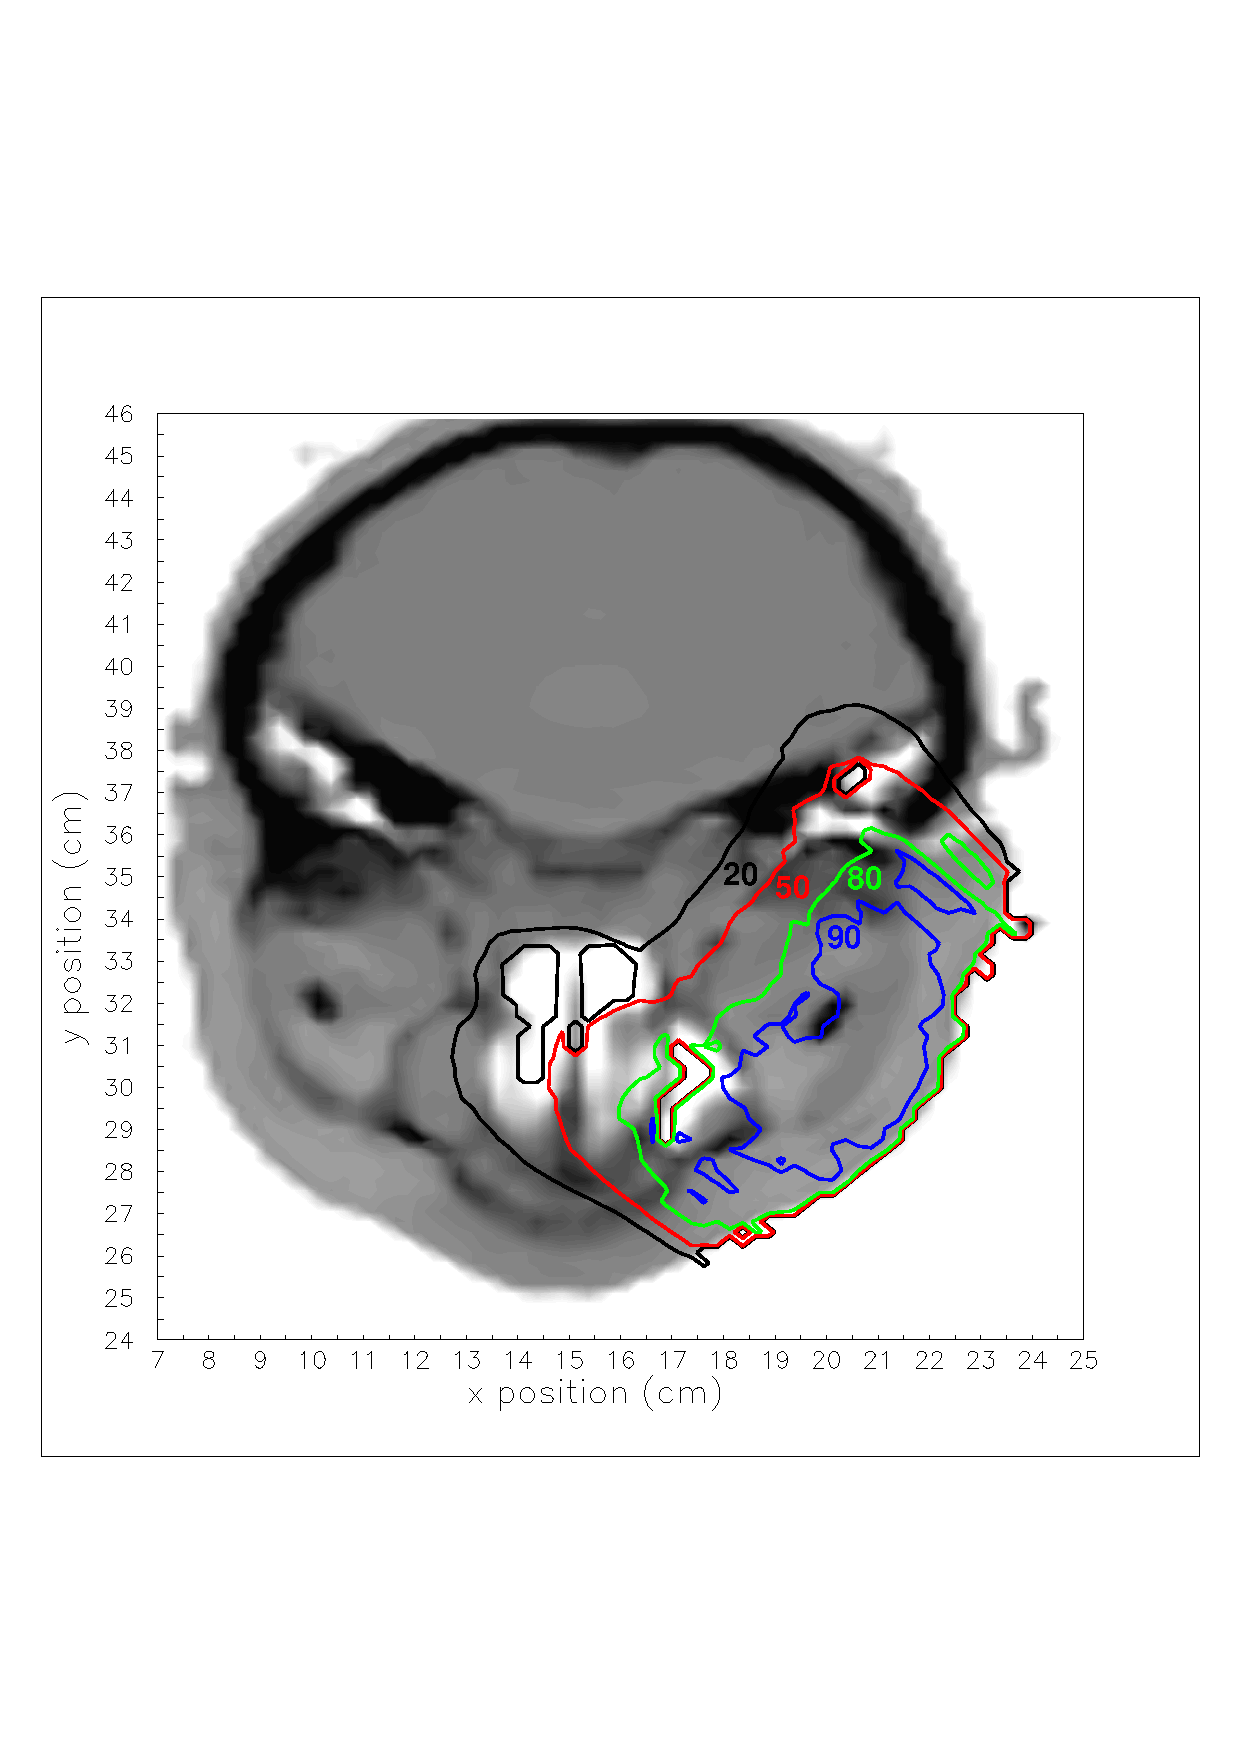
\includegraphics[height=20cm]{figures/CT_example_msmodel}
\end{center}
\end{figure}
\begin{htmlonly}       %%%%%%%%%%%%%%%%%%%%%%%%%%%%%%%%%%%%%%%%%%%%%%
\begin{rawhtml}
</center>
\end{rawhtml}
\end{htmlonly}       %%%%%%%%%%%%%%%%%%%%%%%%%%%%%%%%%%%%%%%%%%%%%%


\vfill
\copyright NRC Canada, 2021
\end{center}

\newpage
\pagestyle{fancy}
\pagenumbering{arabic}
\setcounter{page}{2}

\newpage

\setlength{\parindent}{0em}

\begin{center}
\begin{Large}
{\bf Abstract}
\end{Large}
\end{center}
\indexm{abstract}
DOSXYZnrc is an EGSnrc-based Monte Carlo simulation code for calculating
dose distributions in a rectilinear voxel phantom and is based directly
on the DOSXYZ code developed for the EGS4 code system (see NRC Report
PIRS-509B). DOSXYZnrc is part of the OMEGA-BEAM system of codes developed
at NRC.  Density and material in every voxel may vary.  A variety of beams
may be incident on the phantom, including full phase-space files from
BEAMnrc  and beams characterized using Beam Characterization models. The
companion program {\tt ctcreate} is capable of reading in a CT data set
of Hounsfield numbers and converting it into the information needed by
DOSXYZnrc to simulate transport in a phantom (i.e.  ~the appropriate
material and density are specified in each voxel).  Any of the available
beams can be incident on this CT phantom.  The code includes a resume
option and can be run on parallel computing platforms.  The statistical
analysis is based on a history by history method as opposed to the batch
method used in DOSXYZ.

This user's manual covers general DOSXYZnrc inputs, geometries and outputs.  It
contains information on how to compile and run DOSXYZnrc using the EGSnrcMP
system. It also describes
the use of {\tt ctcreate}.

\begin{latexonly}
\vspace{11.5cm}
\end{latexonly}

\rule{16.3cm}{0.6mm}\\
\begin{small}
The figure on the front page shows a PAW visualisation of the isodose
curves from a DOSXYZ simulation in which a Clinac 2100c 18MeV electron
beam (simulated using a multiple-source model--with 35 million initial
histories) was
incident on the head and neck of a CT phantom.  The visualisation was
implemented by Daryoush Sheikh-Bagheri.

\end{small}

\newpage

\indexm{contents}
\tableofcontents

\newpage

%\pagestyle{myheadings}

\section{Introduction}

\subsection{Overview}
DOSXYZnrc is a general-purpose Monte Carlo EGSnrc\cite{Ka99a,KR00}
\indexm{EGSnrc}
user-code for 3-dimensional absorbed dose calculations. EGSnrc/DOSXYZnrc
simulates the transport of photons and electrons in a Cartesian volume and
scores the energy deposition in the designated voxels. DOSXYZnrc is ``stand
alone'', in the usual EGSnrc sense in that it is controlled by
the {\tt \*.pegs4dat} and {\tt \*.egsinp} files and
is capable of writing out ASCII formatted dose distribution arrays.  The
code uses the EGSnrcMP system which is described in detail in its own
Users Manual\cite{Ka03}.
There is also a graphical user interface (GUI) which allows
input files to be created and executed graphically\cite{TR99}.  Much of the information
in this manual is conveniently accessible via the GUI's help files.


The geometry is a rectilinear volume with
\indexm{geometry coordinate system}
the X-Y plane on the page,  X to the right, Y down the page
and the Z-axis into the page.
Voxel dimensions are completely variable in all three directions. Every
voxel (volume element) can have different materials and/or varying
densities (for use with CT data).  The code allows sources such as a
monoenergetic diverging or parallel beam, phase-space data generated by a
BEAMnrc simulation, or a model-based beam reconstruction produced by BEAMDP.
\indexm{BEAMDP}

DOSXYZnrc has a number of important and unique features such as dose
component calculations, a wide variety of source configurations and beam
reconstruction techniques, CT to phantom conversion
(via {\tt ctcreate}), resume capabilities, phase-space redistribution, \etc.
\indexm{ctcreate}

{\tt ctcreate} is a stand alone program which converts CT data sets into the
data needed for DOSXYZnrc to do a simulation. At present it handles ADAC
Pinnacle, AAPM, CADPLAN and DICOM formats for the CT files.
\indexm{Pinnacle CT}
If you develop extensions, why not
\indexm{CADPLAN CT}
\indexm{DICOM CT}
share them with your colleagues?  Send them to us and we will integrate
them into the standard distribution with full acknowledgement of the
source.

The DOSXYZnrc code, in common with the BEAMnrc system is written for a
preprocessor of Fortran77 called {\tt MORTRAN}. The user does not need
to know {\tt MORTRAN} to use the code, but its elements are needed for
modifications (see refs~\cite{Ne85} or \cite{KR00}).

\subsection{History of DOSXYZnrc}

\indexm{history of DOSXYZnrc}

DOSXYZ started out as a demonstration code that Dave Rogers wrote in March
1986 to show Ralph Nelson that special purpose coding of rectilinear
voxels was faster than using Ralph's more general macros.  At about that time
it was used to estimate the time required to do a full Monte Carlo
treatment planning calculation and the results published 3 years later in
a book chapter\cite{RB90}.  It then became the basis for a Monte Carlo
timing benchmark\cite{BR92} which was regularly updated and available
on the WWW for many years (until 2000).
The OMEGA project took this code over and
added a variety of different source routines with coding contributions
from Charlie Ma, Bruce Faddegon, George Ding, Dave Rogers,  Alex Bielajew,
and Paul Reckwerdt.  More recent modifications have reduced the array
space used by the code, and added beam characterization inputs (Charlie
Ma), btree inputs, (Brian Geiser, but no longer supported), correlated
sampling (Mark Holmes, but no longer supported).
Blake Walters and Mark Holmes added the CT
reading ability in summer 1996.  Blake Walters separated out the
{\tt ctcreate} code in summer 1997 to make the DOSXYZ code much smaller and
thus
able to handle much larger array sizes.  Blake Walters added the
{\tt dsurround} option for reducing simulation time for depth-dose curves
and dose profiles and also the coding for parallel processing in 1998.
\indexm{ctcreate} In 1999, an option was added to allow the user to
run N parallel jobs using a phase space source that exists in N
separate pieces (option now only available using the old
{\tt pprocess} script and not with the new built-in parallel processing
functionality).

Prior to the 1999 revD of this manual, the authors included Paul
Reckwerdt, Mark Holmes and Brian Geiser who had been involved with the
original code to read Pinnacle CT data sets, correlated sampling and
BTREE beam modelling respectively.  These extensions are either no longer
used or are not supported and, thus, these authors are no longer included
as authors of the users manual.  Manuals and/or notes by Geiser and Holmes
are available separately describing BTREE\cite{Ge95} and
correlated sampling\cite{Ho99}.  This latter manual used to be part of
the DOSXYZ Users Manual prior to 1999.

In 2001, with the help of Iwan Kawrakow, Blake Walters ported the
DOSXYZ code to the EGSnrc system to give DOSXYZnrc. At the same time
the statistical analysis routines were converted to a much improved,
history by history approach\cite{Wa02a} instead of the standard batch
approach used in DOSXYZ.

In 2004, Iwan Kawrakow and Blake Walters ported DOSXYZnrc to the new
EGSnrcMP system\cite{Ka03}.  This eliminated the exclusive use of Linux/Unix scripts
and allowed DOSXYZnrc to be compiled and run on Windows-based systems in
addition to Linux/Unix platforms.  At this time, DOSXYZnrc operates
similarly to a standard EGSnrcMP user code, although it is only distributed
as part of the OMEGA/BEAM system.

Although Charlie Ma is no longer an author of the DOSXYZnrc version of the
code, his major contributions to the original EGS4 version still remain.

\vfill

\subsection{Compatibility of DOSXYZ and DOSXYZnrc}

After renaming a DOSXYZ input file from {\tt filename.egs4inp} to {\tt
filename.egsinp}, the file can be used directly by DOSXYZnrc.  This is
because DOSXYZnrc assumes particular default values for all of the
additional EGSnrc input parameters needed.  However, a better approach is
to use the GUI for DOSXYZnrc ({\tt dosxyznrc\_gui}) to read in the DOSXYZ file
and then output the DOSXYZnrc input file with all of the defaults
explicitly stated.  For further information, see
section~\ref{egsnrc_inputs} on page~\pageref{egsnrc_inputs}.

The results of calculations with DOSXYZ and DOSXYZnrc will be very similar
for most situations.  The one systematic difference is that the
relativistic spin corrections to the multiple scattering cause the
depth-dose curves for electron beams to be about 1.5\% more penetrating in
water for a given
electron energy\cite{Wa00}.
\index{DOSXYZ!differences}
\index{DOSXYZ!input file compatibility}
\vfill
\newpage


\section{Compiling/running DOSXYZnrc}
\indexm{compiling!DOSXYZnrc}

\subsection{Files Related to DOSXYZnrc and ctcreate}
\label{filesect}

\indexm{\$HEN\_HOUSE}
As an EGSnrcMP user code, the DOSXYZnrc files are mostly contained in
the directory {\tt \$HEN\_HOUSE/user\_codes/dosxyznrc/},
while {\tt ctcreate} files are
\indexm{ctcreate}
in {\tt \$OMEGA\_HOME/progs/ctcreate/}.  For a general description of the
file structure see Chapter 1 of the BEAMnrc User's Manual \cite{Ro04a}.
\indexm{file structure}

The following describes some files related to DOSXYZnrc:

\begin{description}

\index{dosxyznrc\_gui}
\item[{\tt dosxyznrc\_gui}] This is the Tcl graphical user interface for
creatingi, modifying or executing DOSXYZnrc input files.  Files
related to this are located in
{\tt \$OMEGA\_HOME/progs/gui/dosxyznrc}.  See the GUI manual\cite{TR99}
for more details.
\indexm{graphical user interface}


\item [{\tt egsnrc\_cshrc\_additions} (or {\tt egsnrc\_bashrc\_additions})]
Located in\\ {\tt \$HEN\_HOUSE/scripts}.  If using a Linux/Unix system,
this file must be sourced
in the user's {\tt .cshrc} (or {\tt .bashrc}) file.  It defines useful
aliases for compiling/running DOSXYZnrc.
\indexm{files!egsnrc\_cshrc\_additions}
\indexm{files!egsnrc\_bashrc\_additions}
\indexm{egsnrc\_cshrc\_additions}
\indexm{egsnrc\_bashrc\_additions}

\indexm{Makefile}
\indexm{files!Makefile}
\item [{\tt Makefile}] Located in {\tt \$HEN\_HOUSE/user\_codes/dosxyznrc}.
This file is used by the GNU {\tt make} utility to handle compilation of
\indexm{config.conf}
\indexm{beamnrc.spec}
DOSXYZnrc.  Includes\\ {\tt \$HEN\_HOUSE/specs/config.conf}
(where {\tt config} is the configuration you are using) and
{\tt \$HEN\_HOUSE/specs/beamnrc.spec} files to define environment variables
\indexm{RANDOM}
\indexm{ranmar}
and compiler options.  Also, with the {\tt RANDOM} variable, it defines
the random number generator used (current default is {\tt ranmar}).  Finally,
\indexm{SOURCES}
it defines the variable {\tt SOURCES} which determines the
macros and MORTRAN sources that are
\indexm{mortjob.mortran}
concatenated together to create {\tt mortjob.mortran} (the code that is
actually MORTRAN compiled).
There are two versions of this file, called {\tt Makefile.MS} and  {\tt
Makefile.NOMS}, on the distribution. The default  {\tt Makefile} is  {\tt
Makefile.NOMS} which does not use multiple source models  (source 4, beam
characterization models).  {\tt Makefile.MS} is to be used when Multiple
Source models are to be used (read the file for instructions).
\indexm{beam characterization models}
\indexm{source routines!beam characterization}

\indexm{dosxyznrc.make}
\indexm{files!dosxyznrc.make}
\item[{\tt dosxyznrc.make}] Located in {\tt \$HEN\_HOUSE/user\_codes/dosxyznrc}.  This is an empty file that must exist for compilation using the
{\tt make} utility.

\item[{\tt dosxyznrc.mortran}]  Located in {\tt \$HEN\_HOUSE/user\_codes/dosxyznrc}.  Main {\tt MORTRAN} source code.
\indexm{files!dosxyznrc.mortran}
\indexm{dosxyznrc.mortran}

\item[{\tt srcxyznrc.mortran}]  Located in {\tt \$HEN\_HOUSE/user\_codes/dosxyznrc}.
Subroutines for source configuration inputs + energy spectrum
\indexm{files!srcxyznrc.mortran}
\indexm{srcxyznrc.mortran}

\item[{\tt srcxyznrc.macros}]  Located in {\tt \$HEN\_HOUSE/user\_codes/dosxyznrc}.
{\tt MORTRAN} macros required by {\tt srcxyznrc.mortran}
\indexm{files!srcxyz.macros}
\indexm{srcxyznrc.macros}

\indexm{files!read\_write\_pardose.c}
\indexm{read\_write\_pardose.c}
\indexm{.pardose}
\item[{\tt read\_write\_pardose.c}]  Located in {\tt \$HEN\_HOUSE/user\_codes/dosxyznrc}.  C subroutines used in DOSXYZnrc to
write and read binary {\tt .pardose} output during parallel jobs.  If you
have a C or C++ compiler, then this is compiled when the OMEGA/BEAM
\indexm{read\_write\_pardose.o}
system is installed and {\tt read\_write\_pardose.o} is put
in directory {\tt \$HEN\_HOUSE/lib/config}, where {\tt config} is the
name of your configuration.  If you do not have a C or C++ compiler, then
\indexm{parallel calculations}
this file is not compiled, and the built-in parallel functionality of
DOSXYZnrc cannot be used.

\indexm{files!dosxyznrc\_config.spec}
\indexm{dosxyznrc\_config.spec}
\item[{\tt dosxyznrc\_config.spec}]  (where {\tt config} is the
name of your configuration) Located in\\
{\tt \$HEN\_HOUSE/specs}.  This file is created during OMEGA/BEAM
installation and determines whether or not
the compiled C routines for reading/writing {\tt .pardose} files,
{\tt read\_write\_pardose.o}, are linked in at compile time or not.
If they are to be linked (i.e., you have a C or C++ compiler and
{\tt read\_write\_pardose.c} was compiled successfully), then
\indexm{PARDOSE\_OBJECTS}
the variable {\tt PARDOSE\_OBJECTS} in this file is set
to\\ {\tt \$(EGS\_LIBDIR)read\_write\_pardose.o}, where\\
{\tt \$(EGS\_LIBDIR)}={\tt \$HEN\_HOUSE/lib/config}.  If the
routines are not to be linked at compile time (i.e., you do not
have a C or C++ compiler or {\tt read\_write\_pardose.c} was not
compiled successfully), then {\tt PARDOSE\_OBJECTS} is left blank.

\item[{\tt dosxyznrc\_user\_macros.mortran}] Located in
{\tt \$HEN\_HOUSE/user\_codes/dosxyznrc}.  \\
{\tt MORTRAN} macros that
the user may change  - includes defaults for various options such as beam
models, \etc.  Note that {\tt dosxyznrc\_user\_macros} is also used
by ctcreate to define the maximum dimensions of the DOSXYZnrc phantom
output.
\indexm{files!dosxyznrc\_user\_macros.mortran}
\indexm{dosxyznrc\_user\_macros.mortran}

\item[{\tt dosxyznrc.io}]  Located in {\tt \$HEN\_HOUSE/user\_codes/dosxyznrc}.  This file assigns file names to Fortran unit numbers for output
files not opened explicitly in {\tt dosxyznrc.mortran}.  Currently, the
only files that use this are the {\tt .egslst} file (Fortran unit 1) and
the {\tt .errors} file (Fortran unit 15).
\indexm{files!dosxyznrc.io}
\indexm{dosxyznrc.io}

\indexm{files!phsp\_macros.mortran}
\indexm{phsp\_macros.mortran}
\item[{\tt phsp\_macros.mortran}] {\tt MORTRAN} macros used to read
phase space sources.  This file is always picked up from the
{\tt \$HEN\_HOUSE/utils} directory.

\indexm{files!iaea\_phsp\_macros.mortran}
\indexm{iaea\_phsp\_macros.mortran}
\item[{\tt iaea\_phsp\_macros.mortran}] {\tt MORTRAN} macros used to handle
IAEA-format phase space sources.  Located in the
{\tt \$HEN\_HOUSE/utils} directory, this file is only included if
EGSnrc was installed on a machine with a working C++ compiler and the
library of IAEA phase space handling routines
({\tt \$HEN\_HOUSE/iaea\_phsp/iaea\_phsp.a}) was compiled successfully.
Otherwise, these macros are defined as blank ({\tt \{;\}}) in
{\tt phsp\_macros.mortran} and IAEA functionality does not exist.

\item[{\tt beammodel\_macros.mortran}]    {\tt MORTRAN} macros required
by the multiple-source model for beam reconstruction (source 4), stored in
{\tt \$OMEGA\_HOME/progs/beamdp}.
\indexm{files!beammodel\_macros.mortran}
\indexm{beammodel\_macros.mortran}
\indexm{BEAMDP}

\item[{\tt beammodel\_routines.mortran}]    {\tt MORTRAN} subroutines
required by the multiple-source model for beam reconstruction (source 4),
stored in {\tt \$OMEGA\_HOME/progs/beamdp}.
\indexm{files!beammodel\_routines.mortran}
\indexm{beammodel\_routines.mortran}

\indexm{files!DOSXYZnrc\_examples}
\indexm{DOSXYZnrc\_examples}
\item[{\tt DOSXYZnrc\_examples/}] A subdirectory of
{\tt \$HEN\_HOUSE/user\_codes/dosxyznrc}.  This directory contains sample
input files for DOSXYZnrc.

\end{description}

The following is a description of some of the files related to
{\tt ctcreate}:

\begin{description}

\indexm{files!Makefile}
\indexm{Makefile}
\item[{\tt Makefile}] Located in {\tt \$OMEGA\_HOME/progs/ctcreate}.
Used by the GNU {\tt make} utility, this file
\indexm{SOURCES}
\indexm{mortjob.mortran}
directs the compilation of {\tt ctcreate}.  The {\tt SOURCES} variable defines
the macros and MORTRAN sources concatenated to create {\tt mortjob.mortran}
(which is ultimately MORTRAN compiled)

\item[{\tt ctcreate.mortran}] Located in {\tt \$OMEGA\_HOME/progs/ctcreate}.
This is the main {\tt MORTRAN} source code for
{\tt ctcreate}.
\indexm{files!ctcreate.mortran}
\indexm{ctcreate.mortran}

\indexm{files!ReadCT\_DICOM.c}
\indexm{ReadCT\_DICOM.c}
\indexm{DICOM format}
\item[{\tt ReadCT\_DICOM.c}] Located in {\tt \$OMEGA\_HOME/progs/ctcreate}.
This is a C subroutine for reading CT images in DICOM format.  It is linked
to {\tt ctcreate.mortran} at compile time.

\indexm{files!tags\_ct.h}
\indexm{tags\_ct.h}
\indexm{DICOM format}
\item[{\tt tags\_ct.h}] Located in {\tt \$OMEGA\_HOME/progs/ctcreate}.  This
is a C header file used with {\tt ReadCT\_DICOM.c}.  It defines the
hexadecimal data identifiers used in DICOM image format.

\item[{\tt lnblnk1\_function.mortran}]{\tt MORTRAN} macro to provide the
FORTRAN {\tt lnblnk} function for all configurations.  This is picked
up from {\tt \$HEN\_HOUSE/src}.
\indexm{files!lnblnk1\_function.mortran}
\indexm{lnblnk1\_function.mortran}

\end{description}

\subsection{Compiling and Running DOSXYZnrc}
\label{candrsect}

The commands for compiling and running DOSXYZnrc are
similar to those for other EGSnrcMP user codes
(see the EGSnrcMP Users Manual\cite{Ka03}).
For EGS4 users, please note that file extensions have
changed from, {\em eg,} {\tt file.egs4inp} to {\tt file.egsinp}.
\indexm{.egsinp}
\indexm{.egs4inp}
\indexm{files!.egsinp}
\indexm{files!.egs4inp}

\indexm{DOSXYZnrc!installation}
DOSXYZnrc is normally compiled on your user area as part of the
OMEGA/BEAM user set up
(see the BEAMnrc Manual \cite{Ro04a} for configuration instructions).
To compile DOSXYZnrc independently
(e.g., necessary if you have changed some parameters in \\
{\tt dosxyznrc\_user\_macros.mortran}), ensure that
{\tt Makefile}, {\tt dosxyznrc.make},\\ {\tt dosxyznrc.mortran},
{\tt dosxyznrc\_user\_macros.mortran}, {\tt srcxyznrc.mortran},\\
{\tt srcxyznrc.macros}, and {\tt dosxyznrc.io}
exist in your\\ {\tt \$EGS\_HOME/dosxyznrc} directory (they
should have been copied there automatically from
{\tt \$HEN\_HOUSE/user\_codes/dosxyznrc} during
OMEGA/BEAM configuration).
Then, from {\tt \$EGS\_HOME/dosxyznrc}, compile DOSXYZnrc by typing:
\indexm{make}
\begin{verbatim}
make [options]
\end{verbatim}
The options for {\tt make} are:
\indexm{make!options}
\begin{verbatim}
make              Compile with default optimization
make opt          turned on.  Default optimization is level 2 (-O2).

make noopt        Compile with no optimization

make debug        Compile executable for debugging.

make fortran      Do mortran compilation only, leaving behind the Fortran
                  file dosxyznrc.F.

make clean        Remove the Fortran file, mortjob.mortran file,
                  dosxyznrc.mortlst file and the executable.
\end{verbatim}

\indexm{mf}
\indexm{egsnrc\_cshrc\_additions}
\indexm{egsnrc\_bashrc\_additions}
\indexm{compile\_user\_code}
To preserve compatibility with old usage, the {\tt mf} command is also
available for compiling DOSXYZnrc on a Linux/Unix system (you must have
sourced\\
{\tt \$HEN\_HOUSE/scripts/egsnrc\_cshrc\_additions} or\\
{\tt \$HEN\_HOUSE/scripts/egsnrc\_bashrc\_additions} from your
{\tt .cshrc} or {\tt .bashrc} file).  {\tt mf} is
aliased to the script {\tt \$HEN\_HOUSE/scripts/compile\_user\_code}.

To use {\tt mf}, go into {\tt \$EGS\_HOME/dosxyznrc} and type:
\begin{verbatim}
m[f] dosxyznrc [a] [opt|noopt|debug]
\end{verbatim}
\index{mf!options}
The options for {\tt mf} are:
\verb+mf         =>+ Mortran and Fortran compile and then link\\
\verb+m          =>+ Mortran compile and create the Fortran file\\
\verb+opt        =>+ use optimization (default level 2)\\
\verb+noopt      =>+ use no optimization\\
\verb+debug      =>+ create executable ready for a debug run\\
The parameter ``{\tt a}" is not used and is only present for compatibility
with the previous version of {\tt mf}.

Once you have successfully compiled DOSXYZnrc, the executable,
{\tt dosxyznrc*}, will be left in your {\tt \$EGS\_HOME/bin/config} directory
(where {\tt config} is the name of the configuration that you are using).

\indexm{running DOSXYZnrc}
\indexm{input file}
\indexm{pegs data file}
To run DOSXYZnrc interactively from the command line, go into
{\tt \$EGS\_HOME/dosxyznrc} and type:
\begin{verbatim}
dosxyznrc -i inputfile -p pegsdata
\end{verbatim}
where the input file is {\tt \$EGS\_HOME/dosxyznrc/inputfile.egsinp} and the
file\\
 {\tt pegsdata.pegs4dat} contains the PEGS4 data set (it can be on
{\tt \$EGS\_HOME/pegs4/data} or if not found there, on
{\tt \$HEN\_HOUSE/pegs4/data}).

\index{ex}
If you are using a Unix/Linux system, then you can also start
an interactive DOSXYZnrc run using
the {\tt ex} (aliased to {\tt \$HEN\_HOUSE/scripts/run\_user\_code})
command:
\begin{verbatim}
ex dosxyznrc inputfile pegsdata
\end{verbatim}
{\tt ex} is provided to preserve compatibility with old usage.

\indexm{parallel jobs}
\indexm{batch jobs}
\indexm{running DOSXYZnrc!in batch}
If you are using a Linux/Unix system then you can also run DOSXYZnrc
in batch mode.  Batch submission is required for parallel jobs.
Batch submission uses the {\tt exb} command, which is aliased to
the script {\tt \$HEN\_HOUSE/scripts/run\_user\_code\_batch}.  The syntax
of the {\tt exb} command is:
\begin{verbatim}
exb dosxyznrc inputfile pegsdata [short|medium|long] [batch=batch_sys] [p=N]
\end{verbatim}
\indexm{queues}
\indexm{at} \indexm{NQS} \indexm{PBS} \indexm{keg} \indexm{SGE}
The {\tt [short|medium|long]} option defines the name of the
queue that is used (default is {\tt long} as at NRC).  The {\tt batch\_sys} input
defines the network queuing system to use.  Currently,
{\tt batch\_sys} can be set to {\tt at} (the standard Unix batch
command), {\tt pbs} (to use PBS), {\tt keg} (to use Sun's SGE) or
{\tt nqs} (for NQS).  The default is {\tt at} unless otherwise specified
by setting the environment variable {\tt \$EGS\_BATCH\_SYSTEM}.  Finally,
{\tt N} is used if you are submitting parallel jobs and is set equal to
the number of jobs that you want to split the simulation into.
\indexm{running DOSXYZnrc in parallel}
\indexm{\$EGS\_BATCH\_SYSTEM}

\indexm{temporary working directory}
Once a run is started, a temporary working directory is created as
a subdirectory of\\
{\tt \$EGS\_HOME/dosxyznrc}.  This temporary working directory
has the name\\
{\tt egsrun\_pid\_inputfile\_hostname}, where where {\tt pid} is the process ID number and {\tt hostname} is the name of the
computer the job is running on.  All output files are written
to this temporary directory.  At the end of the run, the files are moved into
{\tt \$EGS\_HOME/dosxyznrc} and the temporary working directory is
deleted.  For more information on temporary working directories, see the
EGSnrcMP Users Manual\cite{Ka03}.

\indexm{.3ddose}
\indexm{files!.3ddose}
\indexm{STATDOSE}
\indexm{output files}
\indexm{.egslst}
\indexm{.pardose}
DOSXYZnrc outputs the following files: {\tt
inputfile.egslst, inputfile.egslog} (for batch runs only, where it
contains screen output), {\tt
inputfile.egsdat} (which can be used to resume the calculation) and {\tt
inputfile.3ddose} which contains a summary of the data in all regions and
can be used by STATDOSE to create {\tt xmgr/xmgrace} graphs (see ``STATDOSE
Users Manual''\cite{MC95} ).  If this is a parallel run, then the
individual jobs will output binary {\tt .pardose} files instead of
{\tt .3ddose} files.  The {\tt .pardose} are then combined automatically at
the end of the parallel run to create a {\tt .3ddose} file.  See section~\ref{parallelcalc} for more information on parallel runs.
Note that the \indexm{inputfile} {\tt
.egslst} file can become VERY long and thereby become useless so use it
carefully for getting the dose which usually can
be more effectively obtained  via the
{\tt .3ddose} output file.
\indexm{xmgrace}
\indexm{xmgr}
\indexm{files!.egslog}
\indexm{.egsinp}
\indexm{files!.egslst}
\indexm{files!.egsdat}
\indexm{.egsdat}
\indexm{.egslog}

\indexm{compiling DOSXYZnrc!from the GUI}
\indexm{running DOSXYZnrc!from the GUI}
\indexm{dosxyznrc\_gui}
The DOSXYZnrc code can also be compiled and run from the
{\tt dosxyznrc\_gui}\cite{TR99}.
To compile DOSXYZnrc, select ``Compile'' from the ``Run'' menu.  This
will open up a window which gives you the different {\tt make} options
(ie optimization vs no optimization, debug, etc).  To run the code
from the GUI, you must first load an existing input file or create a new
one (new inputs or changes to an input file must first be saved before
running).  Then select ``Run'' from the ``Run'' menu.  This will open
up a window in which you can either run DOSXYZnrc interactively
or else submit to a queue (or start a parallel run).  Batch runs will use
the PBS queueing system unless otherwise specified in the
\indexm{\$EGS\_BATCH\_SYSTEM environment\\ variable}
{\tt \$EGS\_BATCH\_SYSTEM} environment variable.  Dialog that would normally
appear on screen during an interactive run now appears in the GUI
run window.

For more information about compiling and running user codes, see the
EGSnrcMP Users Manual\cite{Ka03}.

\subsubsection{Including source 4/beam characterization}

\label{include4}
\indexm{beam characterization models}
\indexm{files!beammodel\_macros.mortran}
\indexm{beammodel\_macros.mortran}
\indexm{files!beammodel\_routines.mortran}
\indexm{beammodel\_routines.mortran}
\indexm{source routines!beam characterization} To implement beam
characterization models in DOSXYZnrc, copy\\ {\tt beammodel\_macros.mortran}
and {\tt beammodel\_routines.mortran}, to the user's {\tt dosxyznrc} area
from {\tt \$OMEGA\_HOME/progs/beamdp}. Also copy {\tt Makefile.MS}
from\\ {\tt \$HEN\_HOUSE/user\_codes/dosxyznrc/} to the user's {\tt
dosxyznrc} area
 and rename it {\tt Makefile}.
Then recompile.
\indexm{BEAMDP}


\subsection{Statistical Analysis}

The statistical analysis in the original DOSXYZ code was done using a standard
batching technique.  Starting with DOSXYZnrc the statistics on the doses are determined by grouping scored quantities
(i.e., energy deposited) on a history-by-history basis
and then determining the uncertainties.
For most sources, this simply means
grouping quantities by incident particle.  However, for phase space sources,
where more than one incident particle may be traced back to a single
primary history, quantities are grouped by primary history.  For more
information, see the published paper on history by history
statistics in DOSXYZnrc and BEAMnrc\cite{Wa02a}.
\indexm{statistics}
\indexm{uncertainties}
\indexm{batch statistics}

It is worth noting that the method used takes into account the latent
variance in any phase space file being used as a source (i.e. the
uncertainty introduced by the statistical variations in the phase space
file). Hence, one cannot reduce the uncertainty in any dose calculation
below that level by recycling the data a large number of times.  However,
one can get an artificially low statistical result which ignores this
latent variance
if the phase space source is allowed to restart the phase space file
instead of using the recycle option (whereby each particle is used multiple
times as it is read in - see section~\ref{nrcycl}, page~\pageref{nrcycl}).
Thus, in order to get accurate uncertainty estimates,
restarting the phase space file should be avoided.
\indexm{NRCYCL}
\indexm{restart phase space}


\section{DOSXYZnrc Input Parameters}
\indexm{input parameters for DOSXYZnrc}

\subsection{Descriptions in DOSXYZnrc Source Code}
\label{DOSXYZ_input}

This section describes input parameters for DOSXYZnrc. The following descriptions
can be found in the beginning of the {\tt dosxyznrc.mortran} source code.
\indexm{graphical user interface}
The graphical user interface facilitates creation of these input files
and contains a great deal of on-line help\cite{TR99}.

\begin{small}
\input{inputs/dosxyznrc.inp}
\end{small}
\clearpage
\section{Source Routines}
\subsection{Source Types in DOSXYZnrc}
\indexm{source routines!summary}
The following source types have been developed for DOSXYZnrc:
\vspace*{-5mm}
\begin{itemize}
\item Parallel rectangular beam incident from the front (isource = 0)
\item Parallel rectangular beam  incident from any direction (isource = 1)
\item Phase-space source, particles incident from any direction
(isource = 2)
\item Point source incident from the front (isource = 3)
\item Beam characterization model, particles incident from any direction
(isource = 4)
\item Uniform isotropically radiating parallelepiped within DOSXYZnrc volume\\
(isource = 6)
\item Parallel rectangular beam incident from multiple angles (isource = 7)
\item Phase-space source incident from multiple angles (isource = 8)
\item Full BEAM treatment head simulation as source (isource = 9)
\item Full BEAM treatment head simulation as source incident from multiple
angles (isource = 10)
\item Phase space source incident
from multiple angles, with multiple SSD's and isocentres--options to run source through a shared library
geometry (defined by BEAM or other MLC code) and synchronize with geometry settings in the case of
a BEAM shared library (isource = 20)
\item BEAM treatment head simulation incident from multiple angles, with multiple SSD's and isocentres--options
to synchronize with BEAM geometry settings and run source through a shared library geometry (other MLC code) (isource = 21)
\end{itemize}
For all sources, the first input record is:\\
{\tt iqin, isource, ......}\\

\clearpage

\subsection{isource = 0: Parallel Rectangular Beam Incident from Front}
\indexm{source routines!isource = 0}
\indexm{source routines!parallel front}

The uniform parallel rectangular beam is always assumed to be incident parallel
to the Z-axis from the front of the phantom. The input parameters are:

\begin{description}
\item [~~~~{\tt iqin}] Charge of the incident beam (-1: electron, 0: photon, 1: positron)
\indexm{iqin}
\item [~~~~{\tt isource}] = 0
\item [~~~~{\tt xinl,xinu}] Lower and upper x-bounds on the phantom surface
\indexm{xinl,xinu}
\item [~~~~{\tt yinl,yinu}] Lower and upper y-bounds on the phantom surface
\indexm{yinl,yinu}
\item [~~~~{\tt thetax}] Angle of the beam relative to the x-axis (degrees)
\indexm{thetax}
\item [~~~~{\tt thetay}] Angle of the beam relative to the y-axis (degrees)
\indexm{thetay}
\item [~~~~{\tt thetaz}] Angle of the beam relative to the z-axis (degrees)
\indexm{thetaz}

\end{description}

\begin{figure}[htbp]
\begin{center}
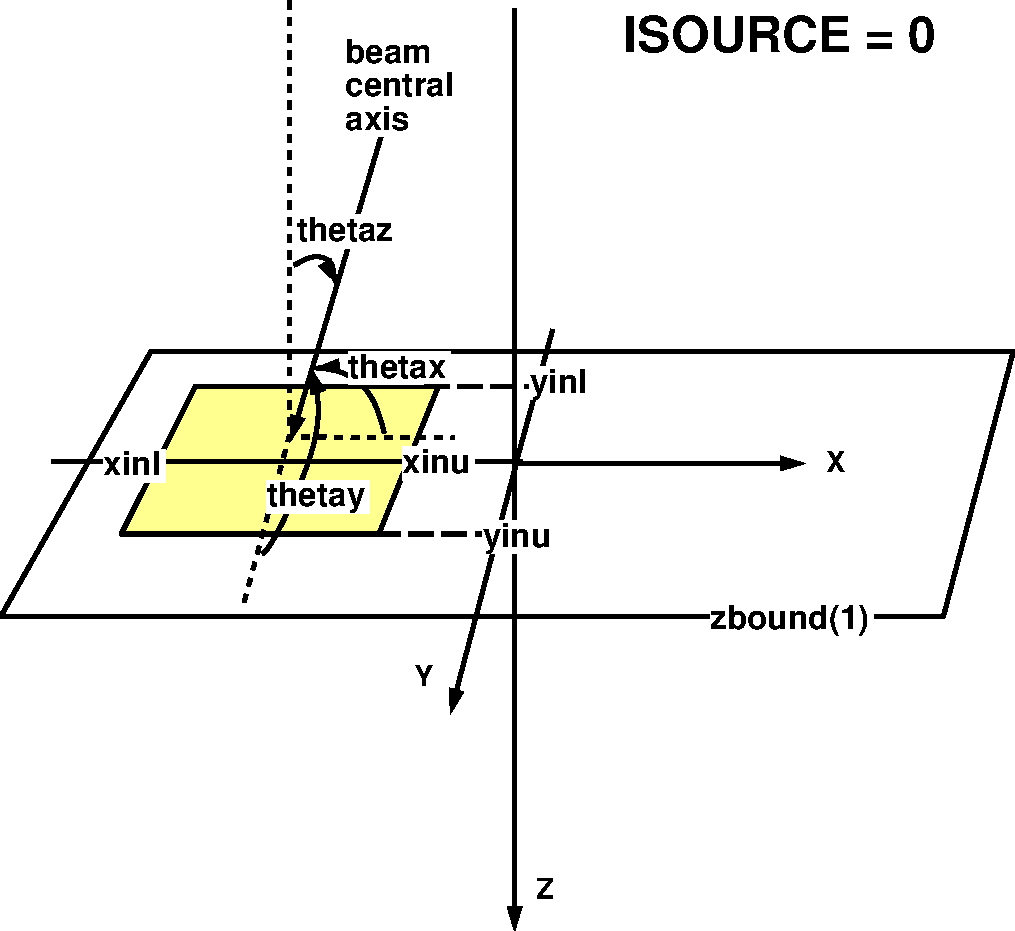
\includegraphics[height=12cm]{figures/src0}
\caption{Parallel rectangular beam (isource=0) showing the beam field, defined by
{\tt xinu}, {\tt xinl, yinu}, and {\tt yinl} on the phantom surface and the
beam directions, {\tt thetax}, {\tt thetay}, and {\tt thetaz}.
The angles {\tt thetax} and {\tt thetay} are relative to the positive x- and y-axes respectively,
while {\tt thetaz} is measured relative to the negative z-axis.}
\label{fig_src0}
\end{center}
\end{figure}
\indexm{xinl,xinu}
\indexm{yinl,yinu}
\indexm{thetax}
\indexm{thetay}
\indexm{thetaz}

\clearpage

\rfoot[]{}

\subsection{isource = 1: Parallel Rectangular Beam Incident from Any Direction}
\indexm{source routines!isource = 1}
\indexm{source routines!parallel any direction}

This uniform parallel rectangular beam may be incident from any direction. The input parameters are:

\begin{description}
\item [~~~~{\tt iqin}] Charge of the incident beam (-1: electron, 0: photon, 1: positron)
\indexm{iqin}
\item [~~~~{\tt isource}] = 1
\item [~~~~{\tt xiso/yiso/ziso}] x-, y-, z-coordinates of the isocenter.  The
isocenter is normally inside the phantom.
\indexm{xiso,yiso,ziso}

\item [~~~~{\tt theta}]   Angle between the +z direction and a line joining
the center of the beam where it strikes the phantom surface to the
isocenter.  In a polar coordinate system, this angle is known as the polar
angle and normally has a range 0-180 degrees.  Note that a centred beam
incident along the +z-axis (ie from the top) has {\tt theta}=180 degrees.
{\tt theta} is
not to be confused with {\tt thetaz} for isource=0, for which case {\tt
thetaz}=0 degrees to aim the source=0 beam along the +z-axis.
\indexm{thetaz}
\indexm{theta}


\item [~~~~{\tt phi}]      Angle  between the +x direction and the
projection on the x-y plane of the line joining the center of the beam on
the phantom surface to the isocenter on the xy plane.  In a polar
coordinate system, this angle is known as the azimuthal angle and normally
has a range 0-360 degrees.
\indexm{phi}

\item [{\tt xcol}/{\tt ycol}]  Total x- and y-widths of the beam on
the plane perpendicular to the beam direction, defined by the center of
the beam and the isocenter
\indexm{ycol}
\indexm{xcol}

\item [{\tt phicol}]  Angle by which the collimator is rotated in the
collimator plane perpendicular to the beam direction.  {\tt phicol} is
determined for {\tt theta}={\tt phi}=0.  The positive sense of rotation is
counterclockwise as one sights down the beam direction.  Note that the
effect of setting {\tt phicol}=90 degrees is the same as switching the
values of {\tt xcol} and {\tt ycol} when {\tt theta} and {\tt phi} are 0
or are both multiples of 90 degrees.
\indexm{theta}
\indexm{phicol}
\end{description}

\clearpage

\rfoot[{\sffamily \rightmark}]{{\sffamily \leftmark}}

\begin{figure}[htbp]
\begin{center}
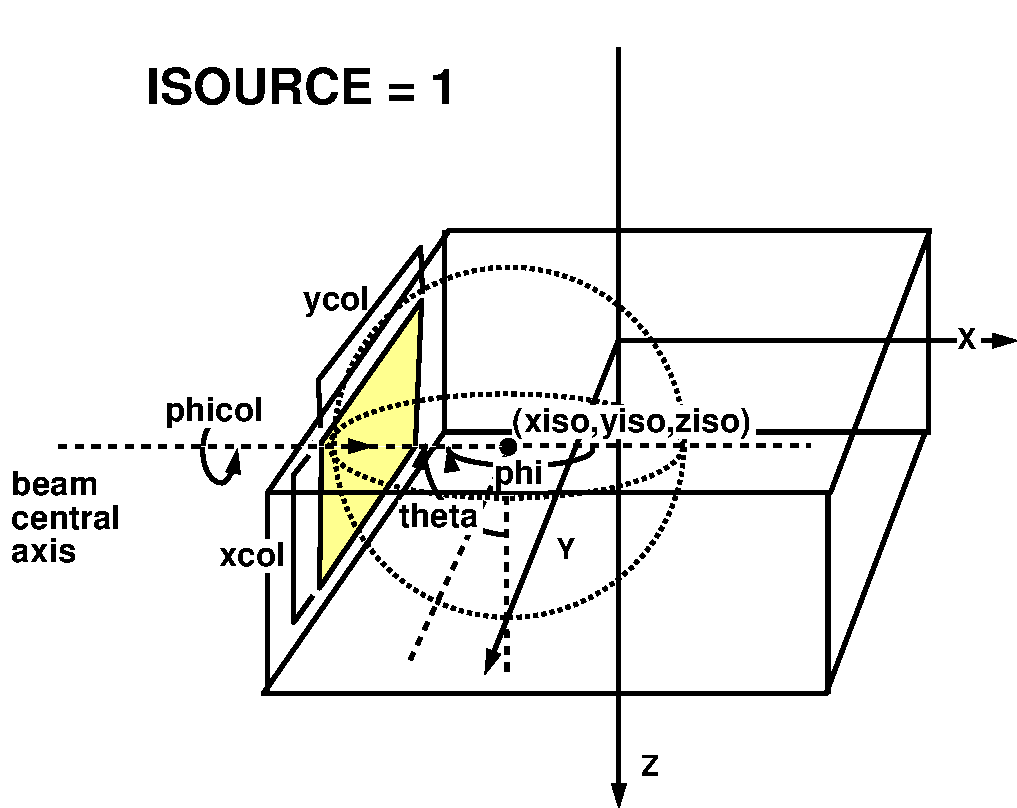
\includegraphics[width=16cm]{figures/src1}
\caption{Parallel rectangular beam incident from any direction (isource=1).  A
polar coordinate system is set up at the isocenter, (xiso,yiso,ziso).  The
position of the beam collimator is then defined using the angles, {\tt
theta} and {\tt phi}.  In the particular example shown in this figure,
with the beam incident on the centre of the negative Y face of the volume,
{\tt theta} is 90 degrees and {\tt phi} is 180 degrees.  The dimensions of
the rectangular collimator are given by {\tt xcol} and {\tt ycol}.  An
additional degree of freedom is available by allowing the collimator to
rotate in its own plane by angle {\tt phicol}.  Note that source 1 is
always incident right on the phantom surface (ie particles do not travel
through air to get to the phantom)}
\label{fig_src1}
\end{center}
\end{figure}
\indexm{xiso,yiso,ziso}
\indexm{theta}
\indexm{phi}
\indexm{phicol}

\clearpage

\subsection{isource = 2: Phase-Space Source Incident from Any Direction}
\label{source2sect}
\indexm{source routines!isource = 2}
\indexm{source routines!phase space}

This source uses a phase-space file generated during a BEAMnrc simulation at
any flat scoring plane of a linear accelerator geometry. A user can choose
any particular type of particles from the phase-space file and score dose
components using the {\tt LATCH} filter. The field size of the incident
\indexm{LATCH} beam can be reduced using the parameter {\tt BEAM\_SIZE}.
There is also a
\indexm{BEAM\_SIZE} parameter called {\tt ISMOOTH} which
can be set to 1 if one wants to shift
\indexm{ISMOOTH} the particles to
their symmetrical positions with respect to x- and y-axis in the
phase-space file for repeated use of these phase-space particles. For {\tt
ISMOOTH} = 0, no shift will be made when phase-space particles are
re-used.  {\tt LATCH} filter, {\tt BEAM\_SIZE} and {\tt ISMOOTH} are input
later in the file.
\indexm{re-use of phase space}

Input parameters for a phase-space source are:
\begin{description}
\item [~~~~{\tt iqin}] Charge of the incident beam (-1: electron, 0:
\indexm{iqin}
            photon, 1: positron, 2: all particle types)
\item [~~~~{\tt isource}] = 2
\item [~~~~{\tt xiso/yiso/ziso}] x-, y-, z-coordinates of the isocenter
\indexm{xiso,yiso,ziso}
                 (normally located within the phantom)
\item [~~~~{\tt theta}]   Same as for isource=1.
\indexm{theta}

\item [~~~~{\tt phi}]     Same as for isource=1.
\indexm{phi}
\item [~~~~{\tt dsource}]      For a BEAMnrc format phase space source, this
is the absolute distance from the isocenter to the
source center, which is, by definition, the origin of the phase-space
plane (origin may not even be in the beam).  For an IAEA format phase
space source, this is the distance from the isocentre to the primary
source ({\it i.e.} the source used to generate the phase space file), or
SAD.
\indexm{dsource}

\item [~~~~{\tt phicol}]  Angle by which the source is rotated in the
                     source plane perpendicular to the beam direction.
                     {\tt phicol} is determined for {\tt theta}={\tt phi}=0.
                     The positive sense of rotation is counterclockwise
                     as one sights down the beam direction.
\indexm{phicol}

\indexm{DBS}
\indexm{directional bremsstrahlung splitting}
\item [~~~~{\tt i\_dbs}] Set to 1 if the phase space source was generated
using directional bremsstrahlung splitting (DBS) in BEAM {\bf AND} you
wish to reject photons directed outside the splitting field (which will
all be fat).  Set to 0 otherwise.  Note that {\tt i\_dbs} is read in as
a real and converted to integer.
\indexm{i\_dbs}

\item [~~~~{\tt r\_dbs}] Radius (in cm) of the DBS splitting field in
the BEAMnrc simulation used to generate this source. Only needed if {\tt
i\_dbs} = 1.
\indexm{r\_dbs}

\item [~~~~{\tt ssd\_dbs}] SSD (in cm) where the DBS splitting field radius
was defined in the BEAMnrc simulation used to generate this source.
Only needed if {\tt i\_dbs} = 1.
\indexm{ssd\_dbs}

\item [~~~~{\tt z\_dbs}] Z value (in cm) in the BEAMnrc simulation
where this phase space source was scored.  This will be at the back of
a component module (CM).  Only needed if {\tt i\_dbs} = 1.
\indexm{{\tt z\_dbs} }

\item [~~~~{\tt e\_split}]  Number of times to split charged particles
as soon as they enter the phantom geometry.  Split particles have their
weight reduced by a factor of 1/{\tt e\_split}.  This is only used
in conjunction with photon splitting ({\tt n\_split}, see Section~\ref{nsplitsect}) and
prevents higher-weight contaminant electrons from compromising statistics
in photon beams.  For maximum efficiency, it is suggested that you
set {\tt e\_split}={\tt n\_split}, the photon splitting number.
\indexm{source 2!charged particle splitting}
\indexm{e\_split}

\indexm{{\tt FILNAM}}
\item [~~~~{\tt FILNAM}] The full name (including extension) of the phase space file
(including the directory path).  In the case of an IAEA-format phase space
source, the full name of the phase space data ({\tt .IAEAphsp}) file
\indexm{IAEA phase space source}
is input here.  The header ({\tt .IAEAheader}) file as assumed to exist
in the same directory.  For more information about IAEA-format date, see
the BEAMnrc Manual.

\end{description}

{\tt theta}, {\tt phi} and {\tt dsource} can be set to place the source
anywhere inside the phantom or the surrounding region; the medium and the
thickness of the surrounding region is input by the user.  Particles from
the phase space which are initially outside both the phantom and surrounding
region are terminated immediately.  If the medium of the surrounding
region is air, for example,  the phase-space particles will be transported
{\it properly} through air to the surface of the phantom. A particle
history is terminated if it is determined that the particle will not make
it to the phantom surface (the particle loses all its energy in the
surrounding region or it escapes through the outer boundaries of the
surrounding region).


Note that, for source 2, the user must set {\tt enflag} = 2 or 3, input
the \indexm{enflag}
mode of the phase-space file (0 or 2), and input the medium number and the
thickness for the surrounding region.  The user should also input the
phase-space file name after the above inputs.  These other inputs are
described in sections 5 and 6 below.  For more information related to
phase-space sources, see the section on phase-space files in the
BEAMnrc User's Manual
\cite{Ro04a}.

The value of {\tt phicol} must be set to 180 degrees in order for the X-Y
coordinates in a BEAMnrc-generated phase space source to map onto the
equivalent X-Y coordinates in DOSXYZnrc.  This is because of the general
coordinate transformation done going from BEAMnrc to DOSXYZnrc.

\subsubsection[DBS Inputs]{Inputs related to directional bremsstrahlung
splitting}
\label{i_dbs_sect}

\indexm{DBS}
\indexm{directional bremsstrahlung splitting}
\indexm{fat photons}
If you have used the directional bremsstrahlung splitting (DBS) variance
reduction technique (see the BEAMnrc User's Manual\cite{Ro04a} for more
details) to
generate the phase space source, then it is recommended that you use
the inputs {\tt i\_dbs}, {\tt r\_dbs}, {\tt ssd\_dbs} and {\tt z\_dbs} to
prevent unsplit, high-weight (``fat") photons which are outside the
splitting field from compromising your dose statistics.
{\tt r\_dbs} and {\tt ssd\_dbs} (the DBS splitting field radius and
SSD in cm) are available directly from the inputs for DBS in the BEAM
simulation, while {\tt z\_dbs} is simply the Z value at the back of the
component module (CM) in the BEAMnrc simulation in which this phase space source was scored.  If
{\tt i\_dbs} is set to 1, then before a photon is used in the DOSXYZnrc
simulation, it is projected along its trajectory from {\tt z\_dbs}
to {\tt ssd\_dbs} (we assume {\tt ssd\_dbs}$\geq${\tt z\_dbs}).  If it
falls outside {\tt r\_dbs} at {\tt ssd\_dbs}, then the photon is
not used in the DOSXYZnrc simulation.  In the context of the BEAM simulation
this photon will not have been split and will be fat (but this information
is not carried in the phase space file except indirectly because of the
larger weight which is not a unique specifier).  To be able to ignore these
fat photons and thereby increase the efficiency considerably, it is
important to ensure that the dose from the photons being ignored is
negligible. This can usually be arranged by making the splitting field big
enough.
\indexm{DBS}
\indexm{directional bremsstrahlung splitting}

Note that charged particles are not
rejected with this technique, which means that if you do not want fat charged
particles to compromise dose statistics (especially near the surface of a
phantom) then you must use the electron splitting option in DBS
(again, see the BEAMnrc User's Manual for more details).

\subsubsection{IAEA format phase space sources}
\label{src2iaeasect}
\indexm{source 2!IAEA format phase space file}
In the case of an IAEA format phase space source, the input, {\tt dsource} (see above), defines the distance
from the primary source ({\it i.e.} the source used to generate the phase space file) to the phantom
isocentre, or SAD.  This is because, unlike BEAMnrc format phase space files, the incident Z-position of
particles is available and read from either the phase space data (in the case of 3-D phase space files) or the header file
(in the case of planar phase space files, such as those scored by BEAMnrc).  The input value of {\tt dsource} is then
subtracted from this Z-position to give the distance along the beam axis from the phantom isocentre to the
particle incident position.

The ability of source 2 to automatically handle IAEA phase space files in which the Z-position for each
particle is scored (3-D data) is particularly useful in cases where the phase space data available for
an accelerator is scored on a non-planar surface (as is the case with the data that Varian has made
available for their TrueBeam accelerators) or when using 3-D phase space data scored by an upstream
DOSXYZnrc simulation (see Section~\ref{phspoutsect}).

\begin{figure}[htbp]
\begin{center}
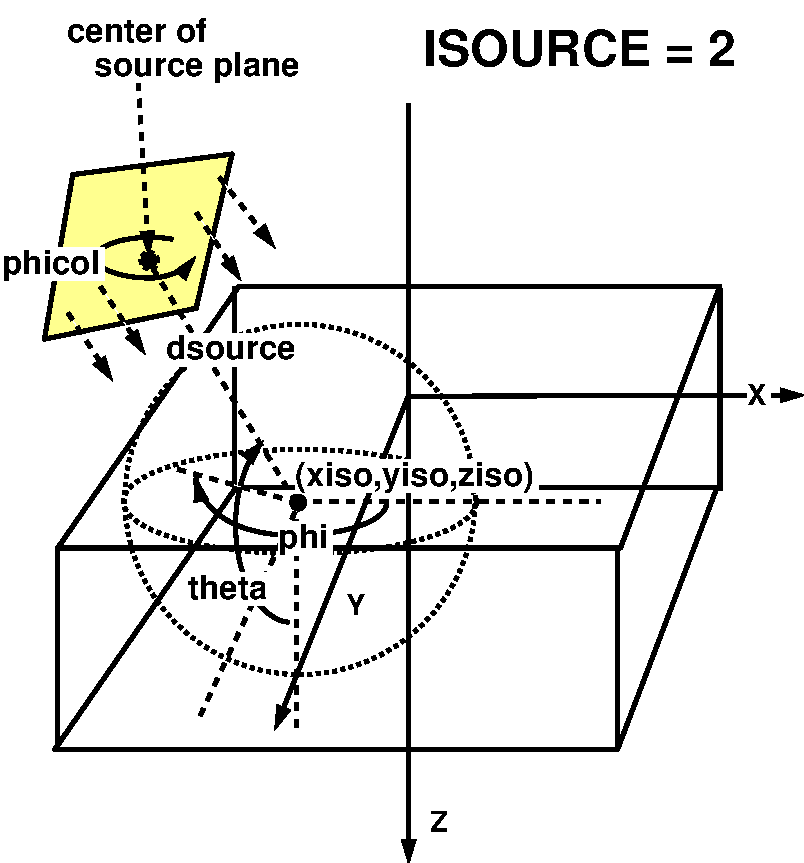
\includegraphics[width=14cm]{figures/src2}
\caption{Phase-space source incident from any direction (isource=2).
Similar to
source 1, a polar coordinate system is set up at the isocenter, (xiso,
yiso, ziso).  The position of the origin in the phase-space plane is then
defined by the angles {\tt theta} and {\tt phi}, and the distance from the
isocenter, {\tt dsource}.  The source can be rotated in its own plane
using the variable {\tt phicol}.  The figure shows that the source plane
does not necessarily have to be right against the surface of the phantom,
however it must be within the surrounding region specified by {\tt dsurround}
 (see section ~\ref{sec5}).}
\label{fig_src2}
\end{center}
\end{figure}
\indexm{dsource}
\indexm{phicol}
\indexm{theta}
\indexm{phi}
\indexm{xiso,yiso,ziso}
\indexm{dsurround}

\clearpage

\subsection{isource = 3: Point Source Rectangular Beam Incident from Front}
\indexm{source routines!isource = 3}
\indexm{source routines!point source rectangle}

The isotropically-radiating point source is placed on the Z-axis.  It is
assumed to be incident on the front surface of the phantom, but can be
placed any distance above the phantom.  The beam field can be asymmetric.

The input parameters for the point source are:
\begin{description}

\item [~~~~{\tt iqin}] Charge of the incident beam (-1: electron, 0:
\indexm{iqin}
                  photon, 1: positron)
\item [~~~~{\tt isource}] = 3
\item [~~~~{\tt xinl,xinu}] Lower and upper x-bounds of the field on the
\indexm{xinl,xinu}
          phantom surface
\item [~~~~{\tt yinl,yinu}] Lower and upper y-bounds of the field on the
\indexm{yinl,yinu}
                   phantom surface
\item [~~~~{\tt ssd}] Distance from the point source to the phantom surface (cm)
\indexm{ssd}
\end{description}

Note that, between the source and the phantom surface the medium is
assumed to be a vacuum for this source.

\begin{figure}[htbp]
\begin{center}
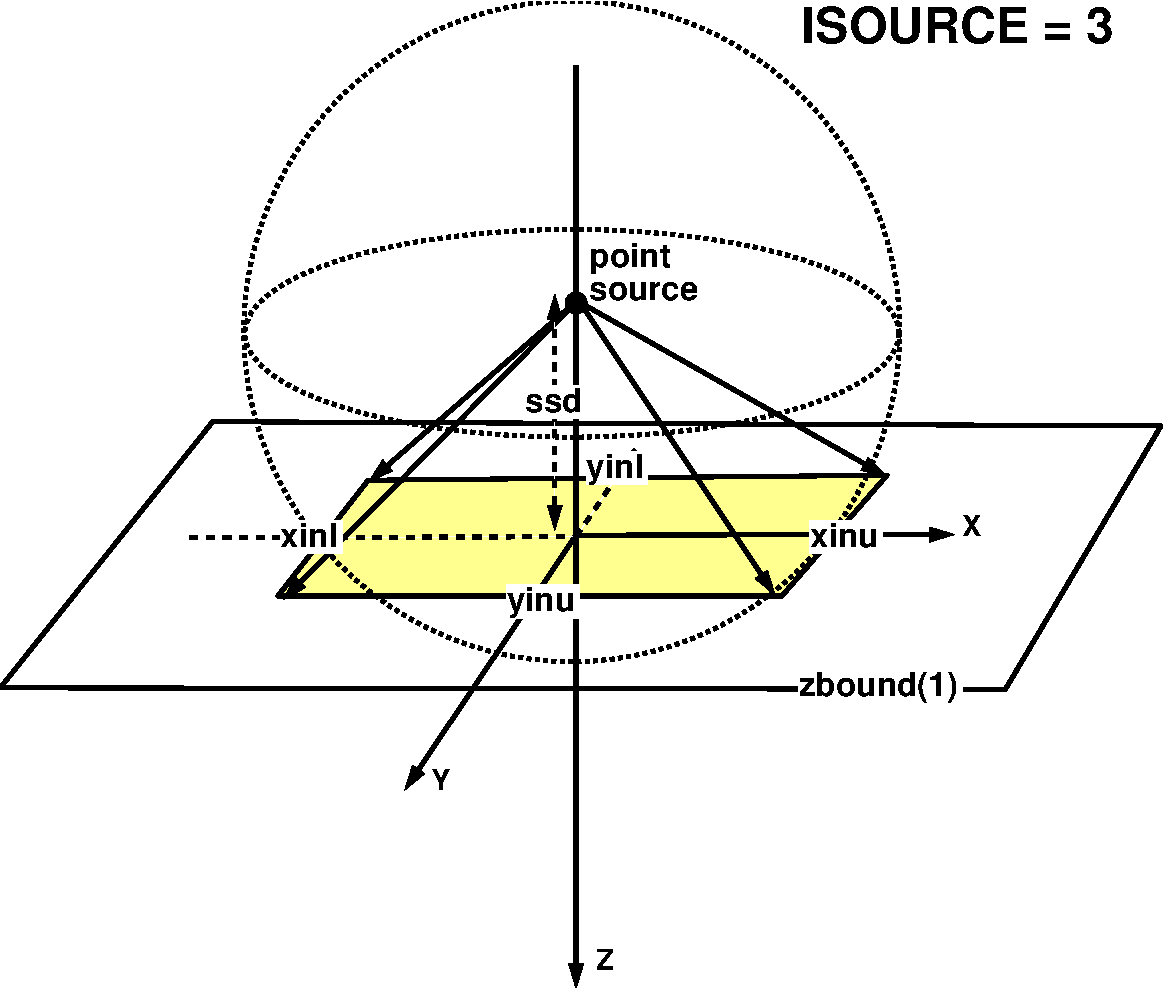
\includegraphics[height=11cm]{figures/src3}
\caption{Point source incident from the front (isource=3).  The
isotropically-radiating point source is located on the Z-axis at distance
ssd above the phantom.  The source is collimated to a rectangular field
defined by xinu, xinl, yinu, yinl on the phantom surface.}
\label{fig_src3}
\end{center}
\end{figure}
\indexm{xinl,xinu}
\indexm{yinl,yinu}

\clearpage


\subsection{isource = 4: Beam Characterization Model Incident
from Any Direction}
\indexm{source routines!isource = 4}
\indexm{source routines!beam characterization}

This source uses the beam characterization models created by BEAMDP from
phase space
data generated by BEAMnrc. This source consists of a variety of sub-sources
for different types of particles coming from different components of a
linear accelerator. Each sub-source has its own spectral and (planar)
fluence distributions and the correlation between the energy, position and
incident angle is retained by sampling the particle positions on the
sub-source (the surface of the component) and on the phase-place plane. A
beam model input file, generated by BEAMDP, is required by this source.
For more details about beam characterization models see the
BEAMnrc User's Manual and associated paper\cite{Ma95c,Ma97}.
\indexm{BEAMDP}

Apart from {\tt isource}, which must be set to 4, input parameters for source 4 are the same as for source 2:

\indexm{enflag}
Note this source requires {\tt enflag} = 4 and to input the beam model
input file name after the {\tt enflag} input. The field size of the
incident beam can be reduced using the parameter {\tt BEAM\_SIZE}.  These
inputs are described in sections 5 and 6 below.
\indexm{BEAM\_SIZE}

The default version of DOSXYZnrc does not include this source. In order to
use it you must recompile DOSXYZnrc using the instructions in
section~\ref{include4}. .

\clearpage

\rfoot[]{}

\subsection{isource = 6: Uniform Isotropically Radiating Parallelepiped
within DOSXYZnrc Volume}
\indexm{source routines!isource = 6}
\indexm{source routines!beam characterization}

This source allows the user to simulate a uniform isotropically radiating
rectangular volume (parallelepiped) within the DOSXYZnrc phantom.
The active volume is restricted to being completely contained within the
DOSXYZnrc phantom.  However, it can be shrunk to a point anywhere within the
phantom.

The input parameters for the uniform isotropically radiating parallelepiped:
\begin{description}

\item [~~~~{\tt iqin}] Charge of the incident beam (-1: electron, 0:
\indexm{iqin}
                  photon, 1: positron)
\item [~~~~{\tt isource}] = 6
\item [~~~~{\tt xinl,xinu}] Lower and upper x-bounds of the active volume (cm)
\indexm{xinl,xinu}
\item [~~~~{\tt yinl,yinu}] Lower and upper y-bounds of the active volume (cm)
\indexm{yinl,yinu}
\item [~~~~{\tt zinl,zinu}] Lower and upper z-bounds of the active volume (cm)
\indexm{zinl,zinu}
\end{description}

\begin{figure}[htbp]
\begin{center}
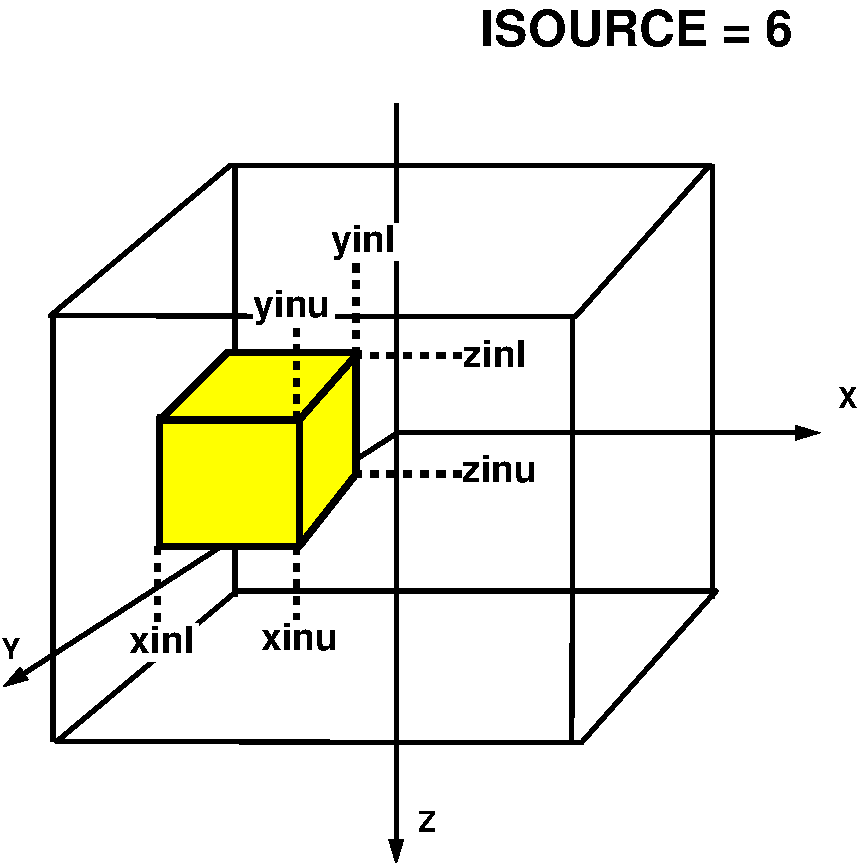
\includegraphics[height=11cm]{figures/src6}
\caption{Uniform isotropically radiating parallelepiped within DOSXYZnrc phantom
(isource=6).  The active volume, specified by {\tt xinl, xinu, yinl,
yinu, zinl, zinu}, must fit within the phantom.  The source can be shrunk
to a point within the phantom by setting {\tt xinu=xinl}, {\tt yinl=yinu}
and {\tt zinl=zinu}.}
\label{fig_src6}
\end{center}
\end{figure}
\indexm{xinl,xinu}
\indexm{yinl,yinu}
\indexm{zinl,zinu}

\clearpage

\subsection{isource = 7: Parallel Rectangular Beam Incident from Multiple Directions}
\label{source7_sec}
\indexm{source routines!isource = 7}
\indexm{source routines!parallel multiple directions}

This is a uniform parallel rectangular beam similar to source 1,
but incident from multiple, user-defined
directions (theta-phi pairs). The input parameters are:

\begin{description}
\item [~~~~{\tt iqin}] Charge of the incident beam (-1: electron, 0: photon, 1: positron)
\indexm{iqin}
\item [~~~~{\tt isource}] = 7
\item [~~~~{\tt xiso/yiso/ziso}] x-, y-, z-coordinates of the isocenter.  The
isocenter is normally inside the phantom.
\indexm{xiso,yiso,ziso}

\item [~~~~{\tt nang}]  The number of incident theta-phi pairs
or, if negative, then abs({\tt nang}) is the number of groups of
incident theta-phi pairs, where, within a group, all theta-phi pairs have
equal probability.  The incident angles theta and phi are defined the
same as they are in source 1.  Theta-phi pairs/groups are specified on
separate lines (see below).
\indexm{nang}
\indexm{theta-phi pairs}

\item [~~~~{\tt xcol}/{\tt ycol}]  Total x- and y-widths of the beam on
the plane perpendicular to the beam direction, defined by the center of
the beam and the isocenter
\indexm{ycol}
\indexm{xcol}

\item [~~~~{\tt phicol}]  Angle by which the collimator is rotated in the
collimator plane perpendicular to the beam direction.  {\tt phicol} is
defined the same way as in source 1.
\indexm{phicol}
\end{description}

And then, on the subsequent {\tt abs(nang)}  lines:\\

{\bf If {\tt nang} $>$ 0:}\\
~~~\\
For i=1,{\tt nang}: {\tt theta(i), phi(i), pang(i)}
\begin{description}
\item [~~~~{\tt theta(i)}]  Theta for pair i (degrees).
\item [~~~~{\tt phi(i)}]  Phi for pair i (degrees).
\item [~~~~{\tt pang(i)}] Probability of particle being incident at
                          Theta(i)-Phi(i).
\indexm{theta(i)}
\indexm{phi(i)}
\indexm{pang(i)}
\end{description}
{\bf If {\tt nang} $<$ 0:}\\
~~~\\
For i=1,-{\tt nang}: {\tt ivary(i), angfixed(i), angmin(i), angmax(i),
ngang(i), pgang(i)}
\begin{description}
\item [~~~~{\tt ivary(i)}] Set to 0 to vary phi in group i; Set to 1 to vary
theta in group i.
\item [~~~~{\tt angfixed(i)}] Fixed theta ({\tt ivary(i)}=0) or phi
({\tt ivary(i)}=1) in group i (degrees).
\item [~~~~{\tt angmin(i)}] Minimum varying phi ({\tt ivary(i)}=0) or
theta ({\tt ivary(i)}=1) in group i (degrees).
\item [~~~~{\tt angmax(i)}] Maximum varying phi ({\tt ivary(i)}=0) or
theta ({\tt ivary(i)}=1) in group i (degrees).
\item [~~~~{\tt ngang(i)}] Number of equally-spaced phi ({\tt ivary(i)}=0) or
theta ({\tt ivary(i)}=1) between and including {\tt angmin(i)} and
{\tt angmax(i)} in group i (Note that, since it includes
{\tt angmin(i)} and {\tt angmax(i)}, {\tt nang(i)} must be $\geq$ 2).
\item [~~~~{\tt pgang(i)}] Probability of particle being in group i.  Within
a group, all theta-phi pairs have equal probability.
\indexm{ivary(i)}
\indexm{angfixed(i)}
\indexm{angmin(i)}
\indexm{angmax(i)}
\indexm{ngang(i)}
\indexm{pgang(i)}
\end{description}

Note that the {\tt pang(i)} are automatically normalized.


\subsection{isource = 8: Phase-Space Source Incident from Multiple Directions}
\label{src8sect}
\indexm{source routines!isource = 8}
\indexm{source routines!phase space from multiple\\ directions}

This source is similar to source 2, except that it is incident from
multiple, user-defined directions (theta-phi pairs).

Input parameters for source 8 are:
\begin{description}
\item [~~~~{\tt iqin}] Charge of the incident beam (-1: electron, 0:
\indexm{iqin}
            photon, 1: positron, 2: all particle types)
\item [~~~~{\tt isource}] = 8
\item [~~~~{\tt xiso/yiso/ziso}] x-, y-, z-coordinates of the isocenter
\indexm{xiso,yiso,ziso}
                 (normally located within the phantom)

\item [~~~~{\tt nang}]  The number of incident theta-phi pairs
or, if negative, then abs({\tt nang}) is the number of groups of
incident theta-phi pairs, where, within a group, all theta-phi pairs have
equal probability.  The incident angles theta and phi are defined the
same as they are in source 2.  Theta-phi pairs/groups are specified the
same way as they are in source 7 (see section~\ref{source7_sec} above).
\indexm{nang}
\indexm{theta-phi pairs}

\item [~~~~{\tt dsource}]      For BEAMnrc phase space files, this
is the absolute distance from the isocenter to the
source center, which is, by definition, the origin of the phase-space
plane (origin may not even be in the beam).  For IAEA phase space files, this
is the primary source to isocentre distance (SAD).
\indexm{dsource}

\item [~~~~{\tt phicol}]  Angle by which the source is rotated in the
                     source plane perpendicular to the beam direction.
                     {\tt phicol} is determined for {\tt theta}={\tt phi}=0.
                     The positive sense of rotation is counterclockwise
                     as one sights down the beam direction.
\indexm{phicol}
\indexm{DBS}
\indexm{directional bremsstrahlung splitting}
\item [~~~~{\tt i\_dbs}] Set to 1 if the phase space source was generated
                     using directional bremsstrahlung splitting (DBS) in
                     BEAMnrc {\bf AND} you wish to reject photons directed outside
                     the splitting field (which will all be fat).  Set to 0 otherwise.
		Note that {\tt i\_dbs} is read in as a real and converted to integer.
\indexm{i\_dbs}
\item [~~~~{\tt r\_dbs}] Radius (in cm) of the DBS splitting field in
the BEAMnrc simulation used to generate this source. Only needed if {\tt
i\_dbs} = 1.  \indexm{r\_dbs}

\item [~~~~{\tt ssd\_dbs}] SSD (in cm) where the DBS splitting field
radius was defined in the BEAMnrc simulation used to generate this
source. Only needed if {\tt i\_dbs} = 1.  \indexm{ssd\_dbs}

\item [~~~~{\tt z\_dbs}] Z value (in cm) in the BEAMnrc simulation
where this phase space source was scored.  This will be at the back of
a component module (CM). Only needed if {\tt i\_dbs} = 1.  \indexm{{\tt
z\_dbs} }

\indexm{e\_split}
\indexm{source 8!charged particle splitting}
\item [~~~~{\tt e\_split}] Number of times to split charged particles
as soon as they enter the phantom.  The weight of split particles
is reduced by a factor of 1/{\tt e\_split}.  This is used in
conjunction with photon splitting (input variable {\tt n\_split}, see
Section~\ref{nsplitsect}) to prevent higher-weight contaminant electrons
from compromising dose statistics.  For optimum efficiency,
set {\tt e\_split}={\tt n\_split}.

\indexm{{\tt FILNAM}}
\item [~~~~{\tt FILNAM}] The full name (including extension) of the phase space
file
(including the directory path).  See the description of
source 2 (Section~\ref{source2sect}) for more details.
\end{description}
An example may help illustrate this input.  The following input:
\typeout{}
\typeout{*******Example end of 4.9 has two extra variables??  *************}
\typeout{*******Example end of 4.9 has two extra variables??  *************}
\typeout{*******Example end of 4.9 has two extra variables??  *************}
\typeout{}
\begin{verbatim}
0, 8, 0.0, 0.0, 0.0, -1.0, 80.0, 90.0, 0.0, 0.0, 0, 0.0, 0.0, 0.0
1, 90.0, 0.0, 356.40, 100, 1.0
\end{verbatim}
is for source 8. The phase space file rotates about the isocenter at
(0,0,0). The centre of the phase-space is 80 cm from the isocenter and the
collimator angle is 90 degrees.
The -1.0 indicates there is only one group of angles. The 1 at the start of
the second line tells us that phi is fixed (at 90 degrees)
and that theta is varying, in
this case in 100 discrete steps between 0 and 356.4 degrees with equal
intensity at each angle.  In this example, {\tt i\_dbs} is set to 0, indicating
that either directional bremsstrahlung splitting (DBS) was not used in the
BEAMnrc simulation that generated this source or else the user does not wish
to reject high-weight (``fat") photons created by DBS.

For more information on how to use the inputs {\tt i\_dbs},
{\tt r\_dbs}, {\tt ssd\_dbs} and {\tt z\_dbs} see section~\ref{source2sect}
on source 2 above.

Similar to source 2, source 8 automatically handles IAEA format phase space sources
with Z-position scored for each particle (3-D phase space).

\subsection{isource = 9: BEAM Treatment Head Simulation Incident from Any
Direction}
\label{src9sect}
\indexm{source routines!isource = 9}
\indexm{source routines!full BEAM simulation}

This source uses particles sampled from a BEAM simulation running
concurrently with the DOSXYZ
\indexm{BEAM accelerator code}
simulation.  The BEAM accelerator code must be compiled as a shared
library (existing in directory {\tt \$EGS\_HOME/bin/config}, where
{\tt config} is the name of your configuration) and must be supplied
with its own input file and pegs data file.  More details about this
are given below.  Source particles for DOSXYZ are then sampled from what
would be the scoring plane during a normal run of the BEAM accelerator.
Thus, this source is similar to {\tt isource}=2 (full phase space file)
without the need to store a phase space file.

\indexm{C/C++ compiler}
\indexm{config.conf file}
\indexm{BEAMLIB\_OBJECTS}
\indexm{BEAMLIB\_EXTRA\_LIBS}
Note that if you are running on Unix/Linux you must have a working C/C++
compiler to use this source and the file
{\tt \$HEN\_HOUSE/specs/config.conf} ({\it i.e.} file {\tt \$EGS\_CONFIG})
must have the variable
{\tt BEAMLIB\_OBJECTS} set to
\indexm{load\_beamlib.o}
{\tt \$(HEN\_HOUSE)lib/\$(my\_machine)/load\_beamlib.o} and\\
{\tt BEAMLIB\_EXTRA\_LIBS} set to {\tt $-$ldl}.
If you have installed EGSnrcMP on a Unix/Linux system with a working C/C++
compiler, the installation will automatically compile the C code
\indexm{load\_beamlib.c}
{\tt \$HEN\_HOUSE/cutils/load\_beamlib.c} to create
{\tt load\_beamlib.o}, and {\tt BEAMLIB\_OBJECTS} and
{\tt BEAMLIB\_EXTRA\_LIBS} will
automatically be set to their proper values.  Otherwise
{\tt BEAMLIB\_OBJECTS} and
{\tt BEAMLIB\_EXTRA\_LIBS} will remain
undefined (ie definitions left blank).

If you are running on Windows, then there is no requirement to have
a working C/C++ compiler to use this source.  In this case, the installation
automatically sets {\tt BEAMLIB\_OBJECTS} in
{\tt \$HEN\_HOUSE/specs/config.conf} to
\indexm{load\_beamlib.obj}
{\tt \$(HEN\_HOUSE)lib/\$(my\_machine)/load\_beamlib.obj}, where
{\tt load\_beamlib.obj} is a precompiled version of {\tt load\_beamlib.o}
included with the installation.  {\tt BEAMLIB\_EXTRA\_LIBS} does not
need to be defined and is left
blank.  See the BEAMnrc Manual\cite{Ro04a} for more information about
{\tt config.conf} files.

Similar to {\tt isource = 2}, you can select particles from the BEAM simulation
\indexm{LATCH}
to use based on their charge and/or {\tt LATCH} values.   You can also
select the maximum size of the BEAM field considered using the
\indexm{BEAM\_SIZE}
{\tt BEAM\_SIZE} input (discussed in more detail in its own section below).

Input parameters for source 9 are:
\begin{description}
\item [~~~~{\tt iqin}] Charge of the incident beam (-1: electron, 0:
\indexm{iqin}
            photon, 1: positron, 2: all particle types)
\item [~~~~{\tt isource}] = 9
\item [~~~~{\tt xiso/yiso/ziso}] x-, y-, z-coordinates of the isocenter
\indexm{xiso,yiso,ziso}
                 (normally located within the phantom)
\item [~~~~{\tt theta}]   Same as for isource=2.  Recall that, for a
beam coming down from the top of the phantom, {\tt theta}=180 degrees.
\indexm{theta}

\item [~~~~{\tt phi}]     Same as for isource=2.
\indexm{phi}
\item [~~~~{\tt dsource}]      Absolute distance from the isocenter to the
centre of the source plane, which is, by definition, the origin of the
scoring plane in the BEAM simulation.
\indexm{dsource}

\item [~~~~{\tt phicol}]  Angle by which the source is rotated about the
                     BEAM central axis.
                     {\tt phicol} is determined for {\tt theta}={\tt phi}=0.
                     The positive sense of rotation is counterclockwise
                     for {\tt theta}=0.  If {\tt theta}=180 degrees
                     (ie beam coming down from the top), then
                     {\tt phicol} must be set to 180 degrees to have the
                     BEAM x-y coordinates match the DOSXYZ x-y coordinates.
\indexm{phicol}

\indexm{DBS}
\indexm{directional bremsstrahlung splitting}
\item [~~~~{\tt i\_dbs}] Set to 1 if directional bremsstrahlung splitting
(DBS) is being used in the BEAM simulation {\bf AND} you wish to reject
fat photons falling outside the DBS splitting field.  This is recommended
so that the fat photons do not compromise dose statistics.  Note that,
with {\tt isource}=9, we have direct access to the BEAM stack variable
({\tt IPHAT}) indicating whether a photon is fat or not, thus we do not
need to reconstruct the DBS splitting field using the additional
inputs {\tt r\_dbs}, {\tt ssd\_dbs} and {\tt z\_dbs} required in
source 2.
\indexm{i\_dbs}

\item [~~~~{\tt e\_split}]  Number of times to split charged particles
as soon as they enter the phantom geometry.  Split particles have their
weight reduced by a factor of 1/{\tt e\_split}.  This is only used
in conjunction with photon splitting ({\tt n\_split}, see Section~\ref{nsplitsect}) and
prevents higher-weight contaminant electrons from compromising statistics
in photon beams.  For maximum efficiency, it is suggested that you
set {\tt e\_split}={\tt n\_split}, the photon splitting number.
\indexm{source 9!charged particle splitting}
\indexm{e\_split}

In addition to the above inputs, the user must input the following
information, all on one line, separated by commas. This line of input
follows the {\tt enflag} input line, {\it i.e.} the second line after the
above input.

\indexm{the\_beam\_code}
\item [~~~~{\tt the\_beam\_code}]  The name of the BEAM accelerator
simulation (ie {\tt BEAM\_accelname}).  This code must have been compiled as
a shared library that exists in your\\ {\tt \$EGS\_HOME/bin/config}
directory.  More information
on compiling a BEAM code as a library is given below.

\indexm{the\_input\_file}
\item [~~~~{\tt the\_input\_file}]  The input file to use for the BEAM
simulation (no {\tt .egsinp} extension).  This file must exist in
your {\tt \$EGS\_HOME/BEAM\_accelname} directory (ie the accelerator
directory).  In the BEAM input file, you must define a single scoring plane
in the accelerator, where
the source particles will be sampled, and the BEAM input
parameter {\tt IO\_OPT} must be set to output a phase space file at
this scoring plane.  See the BEAMnrc Manual\cite{Ro04a} for more information
about scoring planes and {\tt IO\_OPT}.  {\tt the\_input\_file} will
define a value of {\tt NCASE} (no. of histories) for the BEAM simulation,
but this is ignored and the BEAM simulation will always run until
{\tt NCASE} for the DOSXYZ simulation is reached.
\indexm{IO\_OPT}
\indexm{NCASE}

\item [~~~~{\tt the\_pegs\_file}]  The pegs data to be used in the BEAM
\indexm{the\_pegs\_file}
simulation (no {\tt .pegs4dat} extension).  This file must exist in
either {\tt \$HEN\_HOUSE/pegs4/data} or
your\\ {\tt \$EGS\_HOME/pegs4/data} directory.

\end{description}

A graphical representation of source 9 is similar to that of
source 2 shown in Figure~\ref{fig_src2}.  In both sources, the
``source plane'' is the scoring plane in the BEAM simulation, but in source 9
particles are sampled as soon as they cross the scoring plane rather than
stored in a phase space file for later use.  Note that the BEAM central
axis points from the origin of the source plane to the isocenter.

Similar to source 2, {\tt theta}, {\tt phi} and {\tt dsource}
can be set to place the source
plane anywhere inside the phantom or the surrounding region; the medium and the
thickness of the surrounding region are input by the user.  Particles
initially falling outside both the phantom and surrounding
region are terminated immediately. A particle history is terminated if it
is determined that the particle will not make
it to the phantom surface (the particle loses all its energy in the
surrounding region or it escapes through the outer boundaries of the
surrounding region).

The user must also set {\tt enflag} = 2 or 3
the \indexm{enflag}
and input the medium number and the
thickness for the surrounding region.
These inputs are described in sections 5 and 6 below.

\subsubsection[Compiling a BEAM library]{Compiling a BEAM code as
a shared library}
\label{make_library_sect}
\indexm{BEAM shared library}

In order to compile your BEAM accelerator code, {\tt BEAM\_accelname}, as
a shared library, you must already have built the code and created your
\indexm{beam\_build}
directory {\tt \$EGS\_HOME/BEAM\_accelname} using the {\tt beam\_build}
tool.  Building a BEAM code is discussed in detail in the BEAM Manual\cite{Ro04a}.
Of course, if you have already been running {\tt BEAM\_accelname} as a
regular BEAM simulation, then the code will have already been built and
{\tt \$EGS\_HOME/BEAM\_accelname} will exist.  To compile the code as a
shared library, go into your directory \\{\tt \$EGS\_HOME/BEAM\_accelname}
and type:
\indexm{make!BEAM shared library}
\begin{verbatim}
make library
\end{verbatim}
\indexm{BEAM shared library!naming scheme}
If you are using a Unix/Linux system, this will create the
library {\tt libBEAM\_accelname.so}.  On a Windows system, the
library will be named {\tt BEAM\_accelname.dll}.  The library will
automatically be copied to your directory {\tt \$EGS\_HOME/bin/config},
where {\tt config} is the name of your configuration
(e.g. {\tt gcc}, {\tt win2k}, {\tt pgf77}, etc).  See the BEAM Manual for the
differences between the codes concatenated to create a BEAM library and those
used for a standard BEAM accelerator simulation.

\indexm{{\tt libg2c.a}}
In previous versions of BEAMnrc, the library {\tt libg2c.a} was required
when compiling shared library sources on Unix/Linux to avoid confusion of
Fortran units between DOSXYZnrc (the driving code) and BEAMnrc.  Recently,
however, the opening of files in BEAMnrc has been recoded so that only
available Fortran units are used.  This solves the problem of confusion
between Fortran units and eliminates the need for the {\tt libg2c.a}
\indexm{{\tt gfortran}}
library (which caused problems with the {\tt gfortran} compiler).

\indexm{the\_beam\_code}
Recall that when entering the input parameter {\tt the\_beam\_code},
specifying the BEAM simulation to use, you
simply use {\tt BEAM\_accelname}, omitting
the {\tt lib} prefix (in the case of a Unix/Linux library) and
the {\tt .so} or {\tt .dll} extension of the library.

\subsubsection[Efficiency of BEAMnrc simulation source vs. phase space source]
{Efficiency of BEAMnrc simulation source vs. a phase space source}
\indexm{BEAMnrc simulation source!efficiency vs. phase space source}

A BEAMnrc source has the obvious advantage over a phase space source
in that intermediate phase space data need not be stored.  For many
calculations with reasonable precision, this can save tens of
GBytes of disk storage space.  In general, the tradeoff will be a
reduced simulation efficiency, due to the extra
time required to perform a full accelerator simulation to generate
source particles.

Recent research\cite{KW06} has shown, however, that
by using variance reduction techniques in the BEAMnrc simulation
source and in the DOSXYZnrc calculation, the efficiencies of photon
beam dose calculations using BEAMnrc simulation sources can be maximized
so that they are only 3--13\% (depending on beam energy, field size and
phantom voxel size) lower than the peak efficiencies with the equivalent
phase space sources.  The variance reduction techniques required are
directional bremsstrahlung splitting (DBS--see Ref\cite{Ka04a}
and Section 6.3.4 in the BEAMnrc Manual) to maximize the efficiency
of photon production in the BEAMnrc simulation source in conjunction
with
photon splitting ({\tt n\_split}--see Section~\ref{nsplitsect}) to
maximize the efficiency of the DOSXYZnrc calculation.  Efficiencies
quoted for phase space sources include the time required to transport
particles through the accelerator jaws (from ``fixed'' phase space data
collected above the jaws) to generate the source, but even if this
time is omitted, the peak efficiencies with BEAMnrc simulation sources
are only 5--30\% lower than those with phase space sources.

\subsection{isource = 10: Full BEAMnrc Treatment Head Simulation Incident from Multiple Directions}
\indexm{source routines!isource = 10}
\indexm{source routines!BEAMnrc simulation source from\\ multiple directions}

This source is similar to source 9, except that it is incident from
multiple, user-defined directions (theta-phi pairs).

Inputs for source 10 are:
\begin{description}
\item [~~~~{\tt iqin}] Charge of the incident beam (-1: electron, 0:
\indexm{iqin}
            photon, 1: positron, 2: all particle types)
\item [~~~~{\tt isource}] = 10
\item [~~~~{\tt xiso/yiso/ziso}] x-, y-, z-coordinates of the isocenter
\indexm{xiso,yiso,ziso}
                 (normally located within the phantom)

\item [~~~~{\tt nang}]  The number of incident theta-phi pairs
or, if negative, then abs({\tt nang}) is the number of groups of
incident theta-phi pairs, where, within a group, all theta-phi pairs have
equal probability.   Same as for source 8 (see Section~\ref{src8sect} above
for more details).
\indexm{nang}
\indexm{theta-phi pairs}

\item [~~~~{\tt dsource}] Absolute distance from the isocenter to the
centre of the source plane.  Same as for source 9 (Section~\ref{src9sect}).
\indexm{dsource}

\item [~~~~{\tt phicol}] Angle by which the source is rotated about the
                     BEAM central axis.  Same as for source 9 (Section~\ref{src9sect}).
\indexm{phicol}

\indexm{DBS}
\indexm{directional bremsstrahlung splitting}
\item [~~~~{\tt i\_dbs}] Set to 1 if directional bremsstrahlung splitting
(DBS) is being used in the BEAM simulation {\bf AND} you wish to reject
fat photons falling outside the DBS splitting field so that they do not
compromise dose statistics.  Same as for source 9 (Section~\ref{src9sect}).
\indexm{i\_dbs}

\item [~~~~{\tt e\_split}]  Number of times to split charged particles
as soon as they enter the phantom geometry.  This is only used
in conjunction with photon splitting ({\tt n\_split}$>$1).
Same as for source 9 (Section~\ref{src9sect}).
\indexm{source 10!charged particle splitting}
\indexm{e\_split}

\indexm{the\_beam\_code}
\item [~~~~{\tt the\_beam\_code}]  The name of the BEAM accelerator
simulation (ie {\tt BEAM\_accelname}).  Same as for source 9 (Section~\ref{src9sect}).

\indexm{the\_input\_file}
\item [~~~~{\tt the\_input\_file}]  The input file to use for the BEAM
simulation (no {\tt .egsinp} extension).  Same as for source 9.

\item [~~~~{\tt the\_pegs\_file}]  The pegs data to be used in the BEAM
\indexm{the\_pegs\_file}
simulation (no {\tt .pegs4dat} extension).  Same as for source 9.

\end{description}

For an example of how the theta-phi pairs are specified, see the
description at the bottom of Section~\ref{src8sect} above.

Note that, similar to source 9, the user must also set {\tt enflag} = 2 or 3 \indexm{enflag} and input the medium number
and the thickness for the surrounding region. These inputs are described in sections 5 and 6 below.

\subsection{isource = 20: Synchronized phase space source}
\label{src20sect}
\indexm{source routines!isource = 20}
\indexm{source routines!Simulation through moving MLC}
\indexm{source routines!synchronized phase space source}

This source greatly enhances the capabilities of the phase space source incident from multiple directions (isource=8).
Source 20 was developed by Lobo and Popescu\cite{LP10} to allow the user to simulate continuous motion of the phase space
source relative to the DOSXYZnrc phantom over specified ranges of incident
directions, SSD's and isocentre coordinates.  Moreover, the source allows
the user to interpose a geometry, generated using either a BEAM accelerator or a non-EGSnrc code (likely simulating
an MLC geometry) compiled as a shared library, between the source plane and the DOSXYZnrc phantom.  In the case of a BEAM shared library, the source
parameters (range of incident directions, SSD's, isocentres) can be synchronized with the field settings of any synchronized
component modules (see the BEAMnrc Manual\cite{Ro09}).

The geometrical parameters controlling the orientation of the source plane relative to the DOSXYZnrc phantom
have the same definition as those for sources 2, 8, 9 and 10 and are shown in Figure~\ref{fig_src2}.

Input parameters for source 20 are:

\begin{description}
\item [~~~~{\tt iqin}]
\indexm{iqin}
Charge of the incident beam (-1: electron, 0: photon, 1: positron, 2: all particle types)
\item [~~~~{\tt isource}] = 20
\item [~~~~{\tt nset}]
\indexm{nset}
\indexm{\$MXANG}
The number of control points.  Control points define the beginning and end points of ranges of incident direction angles, SSD's and isocentre coordinates over which continuous motion of the source is simulated
(see below).  {\tt nset} must be in the range 2 $\leq$ {\tt nset} $\leq$ {\tt \$MXANG}, where {\tt \$MXANG} is defined in
the file\\ {\tt \$EGS\_HOME/dosxyznrc/dosxyznrc\_user\_macros.mortran}.
\item [~~~~{\tt i\_dbs}]
\indexm{i\_dbs}
Set to 1 if the phase space source was generated using directional bremsstrahlung splitting (DBS) in BEAM and you wish
to reject photons directed outside the splitting field (which will all be fat). Set to 0 otherwise. Note that
{\tt i\_dbs} is read in as a real and converted to integer.
\item [~~~~{\tt r\_dbs}]
\indexm{r\_dbs}
Radius (in cm) of the DBS splitting field in the BEAM simulation used to generate this source. Only needed if {\tt i\_dbs}=1.
\item [~~~~{\tt  ssd\_dbs}]
\indexm{ssd\_dbs}
SSD (in cm) where the DBS splitting field radius was defined in the BEAM simulation used to generate this source. Only needed if
{\tt i\_dbs} = 1.
\item [~~~~{\tt z\_dbs}]
\indexm{z\_dbs}
Z value (in cm) in the BEAM simulation where this phase space source was scored. This will be at the back of a component module (CM). Only needed if {\tt i\_dbs} = 1.
\item [~~~~{\tt e\_split}]
\indexm{e\_split}
Number of times to split charged particles as soon as they enter the phantom geometry. Split particles have their weight reduced by a factor of 1/{\tt e\_split}. This is only used in conjunction with photon splitting ({\tt n\_split}, see Section 8.16) and prevents higher-weight contaminant electrons from compromising statistics in photon beams. For maximum efficiency, it is suggested that you set {\tt e\_split=n\_split}, the photon splitting number.
\item [~~~~{\tt i\_muidx\_out}]
\indexm{i\_muidx\_out}
Set to 1 to include the fractional monitor unit index, {\tt MU}, associated with each particle in IAEA format phase
space output for particles leaving the phantom geometry.  Note that phase space data is not output at all
unless
\indexm{i\_phsp\_out}
{\tt i\_phsp\_out}, the input parameter in the main code controlling phase space output, is set to 1 or 2.
If {\tt MU} is included in the phase space output, then phase space data has a time dimension and is considered 4-D.
Scoring of {\tt MU} allows synchronization between the DOSXYZnrc simulation generating the file and any
downstream simulations--such as BEAMnrc simulations with synchronized component modules--using the file as
a source. See Section~\ref{phspoutsect} for a description of DOSXYZnrc phase space output.
\item [~~~~{\tt calflag}]
\indexm{calflag}
\indexm{NRCYCL}
Set to 1 to skip the calibration run through a BEAM shared library geometry between the source plane and
the phantom. The number of times to recycle each source particle before proceeding to the next one,
{\tt NRCYCL}, will then not take into account the ratio of the number of particles emerging from the
library geometry to the number of incident particles (survival ratio).  The default is to do the calibration run if a BEAM shared library geometry is present.
\end{description}

For i=2,...,{\tt nset} (the no. of control points), the following parameters are entered:
\begin{description}
\item[~~~~{\tt xiso(i)/yiso(i)/ziso(i)}]
\indexm{xiso,yiso,ziso}
x-, y-, z-coordinates of the isocenter.
\item[~~~~{\tt theta(i)}]
\indexm{theta(i)}
Angle of line connecting phase space plane to isocentre relative to the +Z axis.
\item[~~~~{\tt phi(i)}]
\indexm{phi(i)}
Angle of line connecting phase space plane to isocentre relative to the +X axis.
\item[~~~~{\tt phicol(i)}]
\indexm{phicol(i)}
2D Angle of rotation of the phase space plane about its own origin.
\item[~~~~{\tt dsource(i)}]
\indexm{dsource(i)}
The distance from the centre of the phase space plane to the isocentre except when an IAEA format phase space source
is used, in which case input the distance from the primary BEAM source to the isocentre (SAD).  When an IAEA phase space
source is used, the distance from the phase space plane to the isocentre is calculated using the Z position of
the phase space plane read in from the IAEA header file.
\item[~~~~{\tt muIndex(i)}]
\indexm{muIndex(i)}
A monitor unit index in the range $[$0,1$]$ defining the fraction of the total number of incident particles
delivered up to control point i.
Note that {\tt muIndex(i)} $\geq$ {\tt muIndex(i-1)}. Also note that for correct selection of the range
of incident source parameters, {\tt muIndex(i)=0.0} and {\tt muIndex(nset)=1.0}.  See below for more information
on how {\tt muIndex} is used to sample from a range of incident source parameters.
\end{description}
End of inputs required for each control point.

\begin{description}
\item[~~~~{\tt the\_shared\_lib}]
\indexm{the\_shared\_lib}
The name of the BEAM accelerator code or non-EGSnrc MLC simulation code compiled as a
shared library (See below for more information).  Leave this blank if there is no geometry interposed between the
phase space source and the DOSXYZnrc phantom.  This code must have been compiled as a shared library
({\it e.g.} {\tt libBEAM\_accelname.so} if a BEAM accelerator compiled on Unix/Linux) and exist in directory
{\tt \$EGS\_HOME/bin/config}, where {\tt config} is your configuration name.
\item[~~~~{\tt FILNAM}]
\indexm{FILNAM}
The full name (including directory path and file extension) of the phase space source.
\item[~~~~{\tt the\_input\_file}]
\indexm{the\_input\_file}
Input file for the BEAM or non-EGSnrc code defining the shared library geometry interposed between the
phase space source and the DOSXYZnrc phantom.  For a BEAM shared library, this input file must exist in
{\tt \$EGS\_HOME/BEAM\_accelname}   In the case of a BEAM shared library, this file must specify phase space
output at the bottom of the accelerator.
\end{description}

\indexm{MU\_RND}
\indexm{Source 20!Example control point settings}
Prior to each incident particle (Note: not necessarily a statistically-independent primary history)
a random number, {\tt MU\_RND}$\in[$0,1$]$, which can be thought of as a fractional monitor unit, is compared to the {\tt muIndex(i)} of the control points
to determine the incident geometrical parameters.  If source 20 is being run through a BEAM shared library geometry which has
synchronized component modules, such as SYNCJAWS and/or SYNCVMLC (See the BEAMnrc Users Manual\cite{Ro09}), then
the value of {\tt MU\_RND} is passed to BEAM from DOSXYZnrc (more on this below).
If {\tt muIndex(i-1)}$\leq${\tt MU\_RND}$<${\tt muIndex(i)}
then the parameters determining the orientation of the source plane are interpolated
between control points i-1 and i using:

\begin{equation}
{\tt PARAM}={\tt PARAM(i-1)}+\frac{\left[{\tt PARAM(i)}-{\tt PARAM(i-1)}\right]}
{\left[{\tt muIndex(i)}-{\tt muIndex(i-1)}\right]}\left[{\tt MU\_RND}-{\tt muIndex(i-1)}\right]
\end{equation}

Where {\tt PARAM} is the value of the source parameter ({\tt xiso}, {\tt yiso}, {\tt ziso}, {\tt theta}, {\tt phi}, etc) used in the simulation, and {\tt PARAM(i)} and {\tt PARAM(i-1)} are its values defined at control points i and i-1, respectively.
Thus, source parameters are evenly distributed between control points i-1 and i.

The generation of a new value of {\tt MU\_RND} for each incident particle means that particles in the phase space source arising
from the same primary history will be incident from different source orientations.  This was implemented to ensure adequate sampling
of source positions even in cases where where relatively few primary histories are represented in the phase space source
({\it i.e.} if the BEAM simulation used to generate the source used directional bremsstrahlung splitting with a high
splitting number).  Note, however, that regardless of how spatially well-sampled a dose distribution is, its uncertainty is
limited by the number of primary histories simulated.

An simple example input segment for {\tt nset}=7 is:

\begin{verbatim}
0, 0, -9, 90, 0, 0, 15, 0
0, 0, -9, 90, 360, 0, 15, 0.1
0, 0, -5, 90, 0, 45, 15, 0.1
0, 0, -5, 90, 360, 45, 15, 0.5
0, 0, 5, 90, 0, 90, 15, 0.5
0, 0, 5, 90, 360, 90, 15, 0.9
0, 0, 9, 90, 360, 135, 15, 1.0
\end{verbatim}

This sample input defines
four distinct ranges of incident source parameters:

\begin{enumerate}
\item The first two control points ({\tt muIndex(1)}=0.0, {\tt muIndex(2)}=0.1) define 10\% of incident particles
with ({\tt xiso, yiso, ziso})=(0, 0, -9), {\tt theta}=90$^o$ (i.e. incident
from the side of the phantom), {\tt phi} evenly distributed over $[$0,360$^o]$ (i.e. circling the entire phantom in the X-Y plane), {\tt phicol}=0$^o$, and {\tt dsource}=15 cm.
\item Control points 3 and 4, with {\tt muIndex(3)}=0.1 and {\tt muIndex(4)}=0.5, define 40\% of incident particles with
({\tt xiso, yiso, ziso})=(0, 0, -5), {\tt theta}=90$^o$, {\tt phi} evenly distributed over $[$0,360$^o]$, {\tt phicol}=45$^o$, and {\tt dsource}=15 cm.  Note that setting {\tt muIndex(3)} = {\tt muIndex(2)} is used to define a discontinuity between
this range and the previous range, since no parameters will be chosen between control points 2 and 3.
\item Control points 5 and 6, with {\tt muIndex(5)}=0.5 and {\tt muIndex(6)}=0.9, define another range of parameters
(discontinuous with the previous one), in which 40\% of incident particles have
({\tt xiso, yiso, ziso})=(0, 0, 5), {\tt theta}=90$^o$, {\tt phi} evenly distributed over $[$0,360$^o]$, {\tt phicol}=90$^o$, and
{\tt dsource}=15 cm.
\item Control point 7 ({\tt muIndex(7)}=1.0) defines 10\% of particles ({\tt muIndex(7)}-{\tt muIndex(6)}=0.1) with
({\tt xiso, yiso, ziso}) evenly distributed over $[$(0, 0, 5),(0, 0, 9)$]$, {\tt theta}=90$^o$, {\tt phi} evenly distributed over $[$0,360$^o]$, {\tt phicol} evenly distributed over $[$90$^o$,135$^o]$ and {\tt dsource}=15 cm.  Note that this range is
continuous with the previous one.
\end{enumerate}

A realistic simulation of a treatment plan may involve hundreds, or thousands, of control points.  In practice these could
either be extracted from a treatment plan or generated using your own code\cite{LP10}.  Note that a large number of
control points may require you to increase the value of {\tt \$MXANG} in {\tt \$EGS\_HOME/dosxyznrc/dosxyznrc\_user\_macros.mortran} (which defines the maximum value of {\tt nset}) and recompile DOSXYZnrc. \indexm{\$MXANG}

\indexm{i\_dbs}
\indexm{z\_dbs}
\indexm{ssd\_dbs}
\indexm{r\_dbs}
It is recommended that the user set the input {\tt i\_dbs}=1 if directional bremsstrahlung splitting (DBS) was used
to generate the phase space source and they wish to eliminate fat photons, directed outside the splitting field, from
the DOSXYZnrc simulation.  From the BEAM simulation used to generate the phase space source, the user must then input
the DBS splitting radius, {\tt r\_dbs}, the Z-position of the scoring plane, {\tt z\_dbs}, and the SSD used for
DBS, {\tt ssd\_dbs}.  See Section~\ref{i_dbs_sect} for more details.

Just as with other phase space sources (sources 2, 8), source 20 requires setting the input parameter, {\tt enflag}, to 2 or 3
(with or without {\tt LATCH} bit filtering), that the mode of the phase space file (0--no {\tt zlast} scoring, 2--{\tt zlast} scoring) be
input, and that the thickness and medium of the region surrounding the phantom be specified.  See Section~\ref{sec5} for more information.

\index{source 20!incident through a shared library geometry}
\subsubsection{Phase space source incident through a shared library geometry}

\indexm{the\_shared\_lib}\indexm{the\_input\_file}
Using the inputs, {\tt the\_shared\_lib} and {\tt the\_input\_file}, the user is able to interpose
a geometry defined using a code compiled as a shared library between the phase space source and the DOSXYZnrc
phantom geometry.  As mentioned above, the code can be a BEAM accelerator or a non-EGSnrc user code, and
{\tt the\_input\_file} is an input file for the code which defines the geometry parameters (e.g. a BEAM input file).
The compiled shared library ({\it e.g.} {\tt libBEAM\_accelname.so} if the code is a BEAM accelerator and has been compiled
on Unix/Linux) must exist in the {\tt \$EGS\_HOME/bin/config} directory, where {\tt config} is the name of your
configuration.

The system requirements for the use of a shared library geometry are the same as those required for
a BEAM treatment head source and are detailed in Section~\ref{src9sect}.  Instructions on compiling
a BEAM code as a shared library are given in Section~\ref{make_library_sect}.

\index{source 20!BEAM shared library}
\index{source 20!general shared library}
A 2D schematic showing the differences between running source 20 through a BEAM shared library versus a
non-EGSnrc code, {\tt user\_code}, compiled as a shared library is shown in Figure~\ref{fig_src20_1}.

\begin{figure}[htbp]
\begin{center}
\hspace*{-1cm}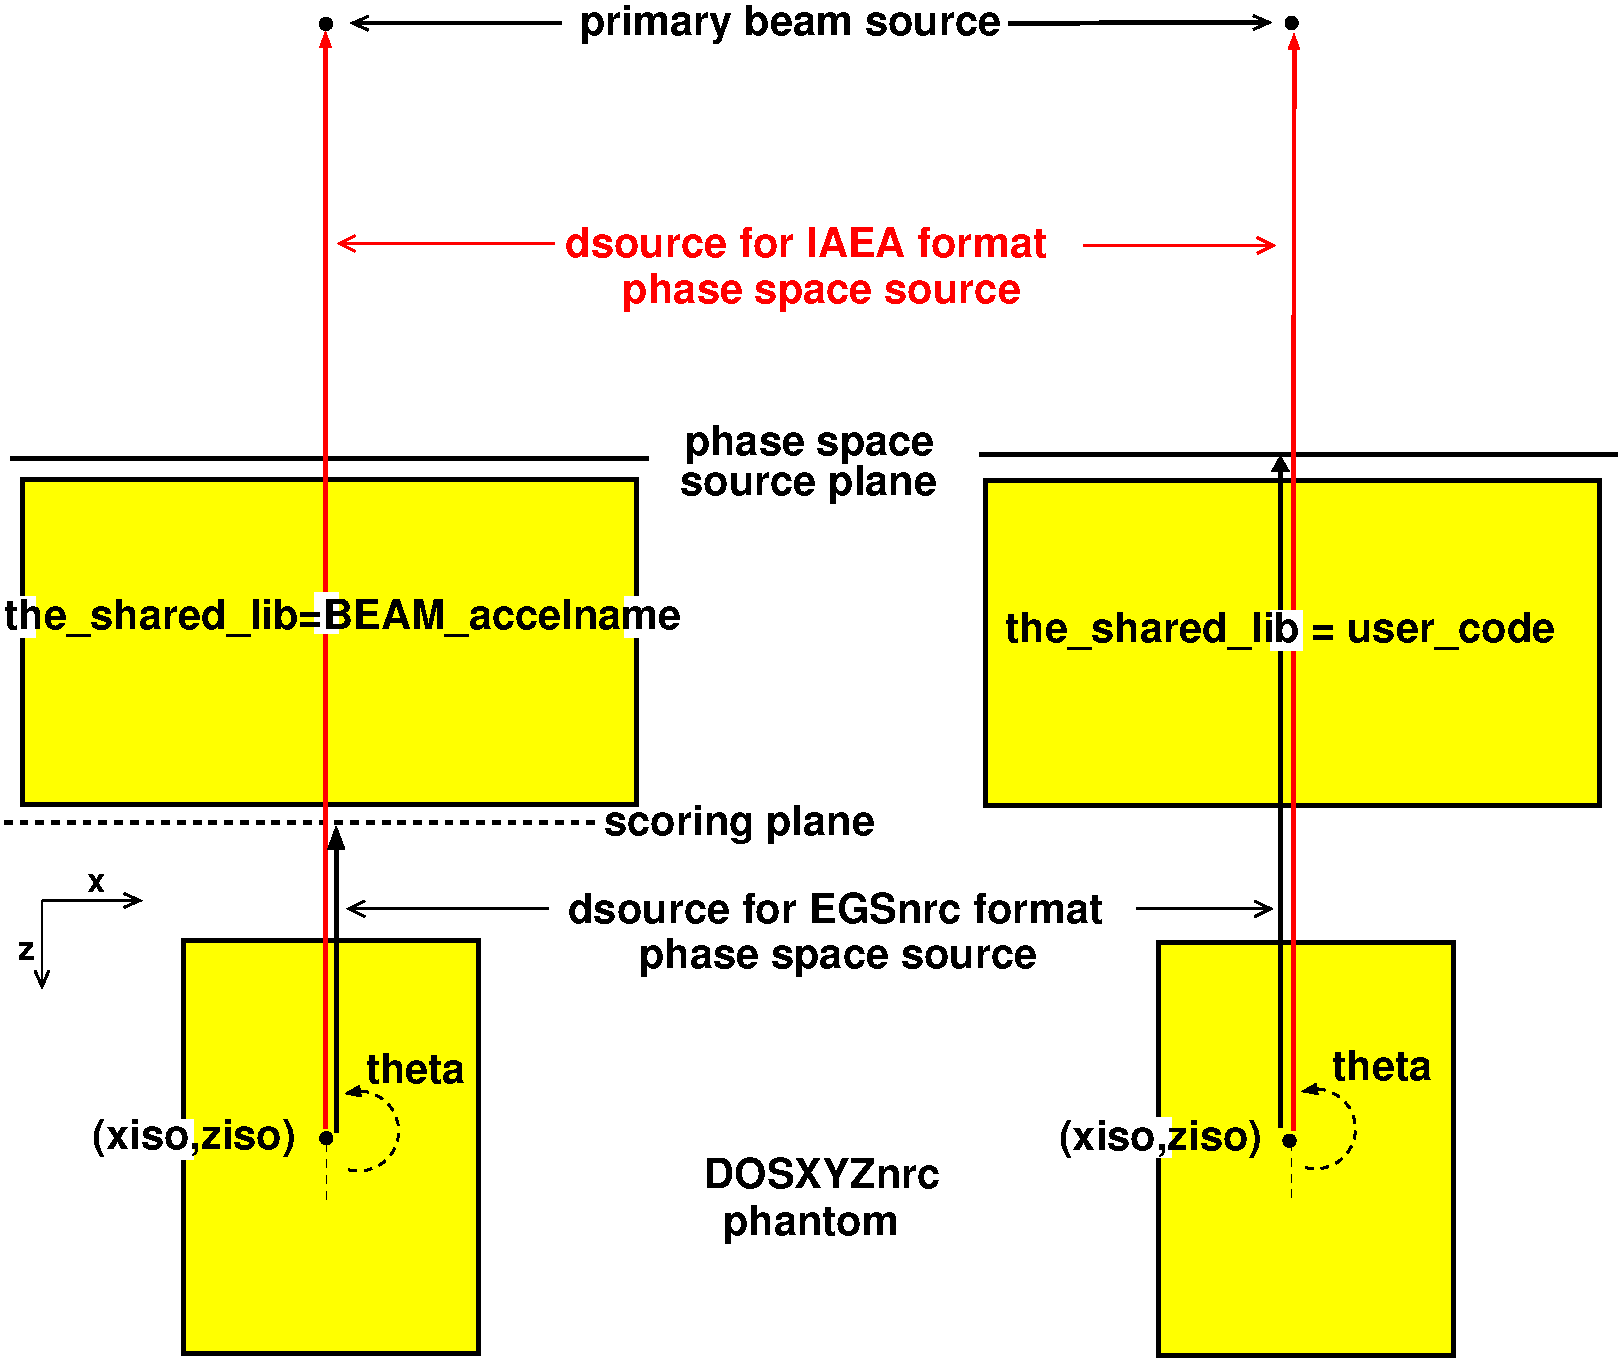
\includegraphics[width=17cm]{figures/src20_1}
\caption{Source 20 incident through a shared library (BEAM or non-EGSnrc user code).  When
the phase space source is run through a BEAM shared library geometry (left), {\tt dsource} defines
the distance between the centre of the scoring plane at the bottom of the geometry and the isocentre (BEAMnrc
phase space source, black arrow), or the distance between the primary source and the isocentre (IAEA phase
space source, red arrow).
When a non-EGSnrc code is used (right), {\tt dsource} defines the distance between the phase space source
and the isocentre (EGSnrc-format phase space source, black arrow) or between the primary source and the isocentre (IAEA phase space
source, red arrow).}
\label{fig_src20_1}
\end{center}
\end{figure}


If a BEAM shared library is used the following conditions apply:
\begin{itemize}
\item The BEAM input file, {\tt the\_input\_file} must define a scoring plane at the bottom of the geometry.  Particle data
at this plane are not actually output but are stored in an internal array for eventual DOSXYZnrc transport through the
phantom.
\item If the source specified in the BEAM input file is a phase space source, it must not make use of the same phase space file as DOSXYZnrc source 20.  This causes a file opening conflict in some versions of
Fortran and will cause the run to fail.  Note that when BEAM is used to define a geometry
for source 20, the BEAM source is not used, so a dummy source of any type can be specified in the BEAM input
file.
\item With a BEAMnrc-format phase space source, the incident Z-position (in the BEAM frame) of the phase space source is
the same as the incident Z-position of the source as defined in the BEAM input file, {\tt the\_input\_file}.  The source 20 input,
{\tt dsource} then defines the distance from the phantom isocentre to the centre of the scoring plane.
\item If an IAEA-format phase space source is used, the incident Z-position of the phase space source is read from
the phase space data itself.  Note that this means the user must ensure consistency between the geometry defined in
BEAM and the incident Z-position of the particles.  The input parameter, {\tt dsource}, defines the distance from
the isocentre to the primary beam source ({\tt i.e.} {\tt dsource}=SAD, see red arrow in figure)
\item The pegs data used in the accelerator simulation is not an input variable and must be the
same as that used in the DOSXYZnrc phantom.
\end{itemize}

If the phase space source is run through a non-EGSnrc shared library (compiled from {\tt user\_code})
the following applies:
\begin{itemize}
\item Phase space data below the defined geometry need not be scored.
\item If a BEAMnrc-format phase space source is used, the incident Z-position (in the {\tt user\_code} frame) is defined
as {\tt dsource}.  Thus, the user must ensure that the source plane is positioned correctly relative to the
defined geometry.
\item For an IAEA-format phase space source, the incident Z-position is read from the phase space source, and
{\tt dsource} defines the primary source-to-isocentre distance.  Again, the user must ensure consistency
between the incident Z-position and the dimensions of the geometry defined in {\tt user\_code}.
\end{itemize}

\indexm{source 20!NRCYCL}
\indexm{source 20!survival ratio}
One issue when running source 20 through a shared library is the determination of how many times
to recycle incident particles so that the phase space source does not rewind, causing loss of information
about particle correlations and subsequent underestimation of dose uncertainties.  As mentioned in Section~\ref{nrcycl}
below, DOSXYZnrc automatically estimates the number of times to recycle each particle, {\tt NRCYCL}, based on
the number of particles in the phase space source, the number of histories requested, and the charge of particles
requested.  However, interactions in the shared library geometry will change the number of particles reaching
the DOSXYZnrc phantom per particle incident from the phase space source.  Thus, the original estimate of
{\tt NRCYCL} is incorrect.  To overcome this when a BEAM shared library is used, an initial calibration comprising
1x10$^6$ particles run through the BEAM geometry only is used to determine the ratio of the number of particles
emerging from the bottom of the BEAM library geometry to the number of incident particles (survival ratio).
{\tt NRCYCL} is then recalculated by multiplying the original estimate by 1/(survival ratio).

\indexm{calflag}
Depending on the shared library geometry, the calibration run can consume
significant CPU time at the beginning of the simulation.  Therefore, if there is a sufficient number of particles in
the phase space source that the user is confident rewinding the source is not an issue, the calibration run can
be skipped by setting the input, {\tt calflag}, to 1.

If a
non-EGSnrc shared library
is used, then the user must provide a routine to estimate the survival ratio of particles passing through the
geometry.  This will be covered in more detail below.

\indexm{synchronized CMs}
When a BEAM shared library geometry includes synchronized component modules (CMs), such as SYNCJAWS, SYNCVMLC or SYNCMLCE,
then the opening coordinates of these component modules (defining the field) can be synchronized with the orientation of the phase space source
plane relative to the phantom.  In this case the value of {\tt MU\_RND}, used to set the incident source orientation (see above), is passed from
DOSXYZnrc to BEAM, where it is then used to set the opening coordinates of any synchronized CMs.
The user controls the synchronization between CM geometries and the incident source orientation using files (one for
each synchronized CM) that associate a field (set of opening coordinates) with a range of fractional monitor units.
See the BEAMnrc Users Manual\cite{Ro09} for more information
about synchronized CMs.

{\bf Non-EGSnrc Geometry Code ({\tt user\_code})}

\indexm{load\_vculib.c}
\index{particleDMLC}
The coding which allows a non-EGSnrc user code compiled as a shared library to communicate with
DOSXYZnrc is found in the C code, {\tt \$HEN\_HOUSE/cutils/load\_vculib.c}. The acronym ``vcu'' stands for
``Virginia Commonwealth University'' and is a reference to the fact that the Lobo and Popescu\cite{LP10}
used a simplified MLC geometry simulation developed at VCU, called {\tt particleDMLC}\cite{Si02}, as a shared
library geometry in simulations with source 20.

\indexm{non-EGSnrc shared library}
\indexm{non-EGSnrc shared library!system requirements}
System requirements for the use of a non-EGSnrc shared library with source 20 (or 21)
are the same as those for a
BEAM simulation source (see Section~\ref{src9sect} above).  Unix/Linux systems must have
a working C/C++ compiler so that {\tt load\_vculib.c} can be compiled to create the
object file, {\tt load\_vculib.o}.  If a working C/C++ compiler is detected on installation
of BEAMnrc/DOSXYZnrc then this is done automatically.  Windows systems do not require
a working C/C++ compiler, since a precompiled version of {\tt load\_vculib.o} is provided.
In addition, the file,
{\tt \$HEN\_HOUSE/specs/dosxyznrc\_config.spec}, where {\tt config} is the configuration
name, must have the
variable {\tt VCULIB\_OBJECTS} set to {\tt \$HEN\_HOUSE/lib/config/load\_vculib.o}
(note that a short form for this is {\tt \$EGS\_LIBDIR/load\_vculib.o})
prior to compiling DOSXYZnrc.  Again, this is set automatically on installation if
{\tt load\_vculib.o} was created successfully.

Currently, {\tt load\_vculib.c} is optimized for calls to subroutines defined in {\tt particleDMLC}. However,
the user can make changes to this file so that it is specific for calls to their own geometry code.  For illustrative
purposes, the following functions must be defined in the user's geometry code, assuming they have made
no changes to {\tt load\_vculib.c} or the DOSXYZnrc coding:

\begin{enumerate}
\indexm{initvcu}
\item{\bf \tt initvcu(char *the\_input\_file, float *survival\_ratio)}
An initialization routine which reads an input file for the geometry code ({\tt the\_input\_file}) and generates
an estimate of the survival ratio of particles between the phase space source and the bottom of the user code
geometry (usually a simulation of an MLC).  The input file would likely specify the geometry parameters and
would also pass the name of the phase space source to the user code.
The survival ratio is used to calculate the number of
times to recycle incident particles, {\tt NRCYCL} (see above).
\indexm{vculib\_sample}
\item{\bf \tt vculib\_sample(float *e, float *x, float *y, float *z, float *u, float *v, float *w, float *wt, int *iq,
 int *latch, int *nhist, int *more\_in\_container)}
A subroutine used to run the geometry code and sample particles reaching the bottom of the geometry.
The subroutine returns the phase space data for a particle at the bottom
of the geometry ({\tt e}=energy; {\tt x,y,z}=particle x,y,z-position; {\tt u,v,w}=x,y,z-direction cosines;
{\tt wt}=particle weight; {\tt iq}=charge; {\tt latch}=latch value), the number of primary histories
run to that point, {\tt nhist}, and an integer, {\tt more\_in\_container}, which is set to 0 if the storage
array for particles reaching the bottom of the geometry is empty ({\tt i.e.} the geometry simulation must
be run on the next call to {\tt vculib\_sample}).
\indexm{vculib\_finish}
\item{\bf \tt vculib\_finish()}
A subroutine called at the end of the simulation to close any files used by the geometry code, free up
reserved memory, etc.
\end{enumerate}

\indexm{source 20!IAEA phase space source}
\label{src20iaeasect}
\subsubsection{IAEA-format phase space sources}

Similar to other phase space sources (sources 2 and 8) source 20 is implemented such that if an IAEA-format phase space source is used, the
incident Z-position of
a particle is automatically read directly from the phase space data.  This eliminates the restriction imposed by BEAMnrc-format
phase space files of all particles being incident in the same plane and, thus, allows more flexibility
in terms of the phase space data that can be used.

\indexm{MU}
\indexm{MU\_RND}
If the IAEA phase space source includes the fractional monitor unit index, {\tt MU}, associated with each particle ({\it i.e.} 4-D data), then
a random value for {\tt MU}, {\tt MU\_RND}, is not chosen at the beginning of each history, and, instead, the value of
{\tt MU} read from the phase space data is automatically
used to set the incident source parameters (isocentre position, incident angle, etc) for the incident particle.
{\tt MU} is automatically
scored in IAEA phase space data output by BEAMnrc simulations using synchronized component modules (CMs) with time-varying opening coordinates
(see the BEAMnrc Users Manual\cite{Ro09}) and can also be included in IAEA phase space data output by DOSXYZnrc
simultions using synchronized sources (20 or 21) by using the {\tt i\_muidx\_out} input flag
(see description of input above and Section~\ref{phspoutsect}).  Thus, use of {\tt MU} read from
the phase space source allows synchronization of source 20 with upstream BEAMnrc simulations having synchronized
CMs or upstream DOSXYZnrc simulations with synchronized sources.

\indexm{spiral CT scan}
\subsubsection{Simulation of Spiral CT Scan}

A recent publication by Kim et al\cite{Ki13} details a modification of Source 8 (See Section~\ref{src8sect} above)
in which the phase space plane can be made to rotate in {\tt phi} about an isocentre which is concurrently
translating in Z, thus simulating exposure in a helical pattern.  Kim et al have used this to simulate dose due
to a spiral CT scan, and their results compare well with measurement.

Spiral scans can be modeled equally well using Source 20 (and 21, see below) using just two control points ({\tt nset}=2).
An example of two control points defining a spiral scan is:

\begin{verbatim}
0, 0, 0, 90, 0, 0, 15, 0
0, 0, 10, 90, 3600, 0, 15, 1.0
\end{verbatim}

These control points define simultaneous translation of the isocentre from {\tt z(1)}=0 to {\tt z(2)}=10 cm and rotation of the source plane
from {\tt phi(1)}=0 at {\tt z(1)} through {\tt phi(2)}=3600$^o$ at {\tt z(2)}.  The angular range, {\tt phi(2)}-{\tt phi(1)}, determines the
pitch of the helix.  In this example, the source rotates ten times (3600$^o$=10$\times$360$^o$) over a Z translation of 10 cm, so the pitch is
equal to 1.  The direction of rotation is determined by the sign of {\tt phi(2)}-{\tt phi(1)}.
If this is positive (as in this example), then rotation is clockwise about the Z-axis; if negative, rotation is counter-clockwise.  Note that the X- and Y-positions of the isocentre in this example remain unchanged, and {\tt theta} is fixed
at 90$^o$, which means the source-isocentre vector is perpendicular to the Z-axis.

The two control points in this example cover the entire range of fractional monitor units ({\it i.e.} {\tt muIndex(1)}=0, {\tt muIndex(2)}=1.0), and, thus,
include all incident particles.
However, using more control points to further subdivide the range, $[$0,1$]$, of fractional monitor units, it would be
possible to generate multiple spiral scans--having different pitch, Z-range, etc--in one simulation.

\subsection{isource = 21: Synchronized BEAM Simulation Source}
\label{src21sect}
\indexm{source routines!isource = 21}
\indexm{source routines!Synchronized BEAM Simulation Source}

Source 21 defines a BEAM treatment head simulation (compiled as a shared library) source incident over multiple ranges
of continuous motion with respect to angle, SSD and isocentre.  The source motion can be synchronized with the settings
of any synchronized component modules (CMs) in the accelerator.  There is also an option to run the source through
a geometry (usually MLC) defined by a non-EGSnrc user code, compiled as a shared library, placed between the treatment
head and the DOSXYZnrc phantom.  Source 21 was developed and contributed by Lobo and Popescu\cite{LP10}.  Just as
source 20 represents a significant enhancement over source 8 (phase space incident from multiple angles), source 21
represents a significant enhancement over source 10 (treatment head incident from multiple angles).

\indexm{source 21!system requirements}
The system requirements for running shared library sources are given in Section~\ref{src9sect} describing source 9 (BEAM
treatment head source incident from one direction).  Instructions on compiling a BEAM accelerator as a shared library
are also given there.

The input parameters for source 21 are:

\begin{description}
\item [~~~~{\tt iqin}]
\indexm{iqin}
Charge of the incident beam (-1: electron, 0: photon, 1: positron, 2: all particle types)
\item [~~~~{\tt isource}] = 21
\item [~~~~{\tt nset}]
\indexm{nset}
\indexm{\$MXANG}
The number of control points defining ranges of continuous source motion.  Same as for source 20 (see above).
{\tt nset} must be in the range 2 $\leq$ {\tt nset} $\leq$ {\tt \$MXANG}, where
{\tt \$MXANG} is defined in
the file {\tt \$EGS\_HOME/dosxyznrc/dosxyznrc\_user\_macros.mortran}.
\item [~~~~{\tt i\_dbs}]
\indexm{i\_dbs}
Set to 1 if directional bremsstrahlung splitting is used in the BEAM simulation and you wish
to reject photons directed outside the splitting field (which will all be fat). Set to 0 otherwise. Note that
{\tt i\_dbs} is read in as a real and converted to integer.
\item [~~~~{\tt e\_split}]
\indexm{e\_split}
Number of times to split charged particles as soon as they enter the phantom geometry. Split particles have their weight reduced by a factor of 1/{\tt e\_split}. This is only used in conjunction with photon splitting ({\tt n\_split}, see Section 8.16) to prevent higher-weight contaminant electrons from compromising statistics in photon beams. For maximum efficiency, it is suggested that you set {\tt e\_split=n\_split}, the photon splitting number.
\item [~~~~{\tt i\_muidx\_out}]
\indexm{i\_muidx\_out}
Set to 1 to include the fractional monitor unit index, {\tt MU}, associated with each particle in IAEA format phase
space output for particles leaving the phantom geometry.  Note that phase space data is not output at all
unless
\indexm{i\_phsp\_out}
{\tt i\_phsp\_out}, the input parameter in the main code controlling phase space output, is set to 1 or 2.
If {\tt MU} is included in the phase space output, then phase space data has a time dimension and is considered 4-D.
Scoring of {\tt MU} allows synchronization between the DOSXYZnrc simulation generating the file and any
downstream simulations--such as BEAMnrc simulations with synchronized component modules--using the file as
a source. See Section~\ref{phspoutsect} for a description of DOSXYZnrc phase space output.
\end{description}

For control points i=1,2,...,{\tt nset}, the following parameters defining the source orientation are entered:
\begin{description}
\item[~~~~{\tt xiso(i)/yiso(i)/ziso(i)}]
\indexm{xiso,yiso,ziso}
x-, y-, z-coordinates of the phantom isocenter.
\item[~~~~{\tt theta(i)}]
\indexm{theta(i)}
Angle of normal connecting origin of the BEAM scoring plane to the isocentre.
\item[~~~~{\tt phi(i)}]
\indexm{phi(i)}
Angle of normal connecting the origin of the BEAM scoring plane to isocentre relative to the +X axis.
\item[~~~~{\tt phicol(i)}]
\indexm{phicol(i)}
2D Angle of rotation of the BEAM scoring plane about its own origin.
\item[~~~~{\tt dsource(i)}]
\indexm{dsource(i)}
The length of the normal from the origin of the BEAM scoring plane to the isocentre.
\item[~~~~{\tt muIndex(i)}]
\indexm{muIndex(i)}
A monitor unit index in the range $[$0,1$]$ defining the fraction of the total number of incident primary histories
delivered up to control point i.  This is slightly different from source 20, where {\tt muIndex(i)} defines the fraction
of incident particles up to control point i.  Thus, for source 21, {\tt muIndex(i)} is actually related to the fractional
monitor units delivered by the BEAM simulation.
Note that {\tt muIndex(i)} $\geq$ {\tt muIndex(i-1)}. Also note that for correct selection of the range
of incident source parameters, {\tt muIndex(1)=0.0} and {\tt muIndex(nset)=1.0}.
\end{description}
This is the end of inputs required for each control point.

\begin{description}
\item[~~~~{\tt the\_beam\_code}]
\indexm{the\_beam\_code}
The name of the BEAM accelerator code ({\it i.e.} {\tt BEAM\_accelname}) used to run the treatment head
simulation.  This must have been compiled as shared library ({\it e.g.} {\tt libBEAM\_accelname.so} on a Linux/Unix system) existing
in your {\tt \$EGS\_HOME/bin/config} directory.
\item[~~~~{\tt the\_input\_file}]
\indexm{the\_input\_file}
The input file for the BEAM treatment head simulation.  This must exist in directory {\tt \$EGS\_HOME/BEAM\_accelname} and must
specify a single scoring plane (usually at the bottom of the accelerator).
\item[~~~~{\tt the\_pegs\_file}]
\indexm{the\_pegs\_file}
The PEGS data to be used in the BEAM treatment head simulation.
\indexm{the\_vcu\_code}
\item[~~~~{\tt the\_vcu\_code}]
This optional input is the name of a non-EGSnrc user code, compiled as a shared library, that can be used to define a geometry
through which particles are run between the bottom of the treatment head and the DOSXYZnrc phantom.  The shared library must
exist in directory {\tt \$EGS\_HOME/bin/config}
\indexm{the\_vcu\_input\_file}
\item[~~~~{\tt the\_vcu\_input\_file}]
Input file for {\tt the\_vcu\_code} defining the geometry interposed between the treatment head simulation and the phantom.
\end{description}

\indexm{\tt MU\_RND}
For each primary history in the treatment head simulation a random fractional monitor unit index, {\tt MU\_RND}$\in[$0,1$]$, is
chosen.  {\tt MU\_RND} is either generated by DOSXZYnrc or, if there are synchronized CMs in the treatment head simulation also
undergoing motion, it is passed to DOSXYZnrc from the BEAM simulation.  More details on the use of synchronized CMs in the BEAM
simulation are given below.  For all particles associated with a given value of {\tt MU\_RND}, the control points, i-1 and i,
within which the source position falls are those for which {\tt muIndex(i-1)}$\leq${\tt MU\_RND}$<${\tt muIndex(i)}, and the
parameters determining the source orientation are calculated using Equation (1) (see Section~\ref{src20sect} above).
Note that, unlike source 20, {\tt MU\_RND} is chosen only for each primary history, not for each incident particle.  Thus,
the {\tt muIndex(i)} for the control points are traceable to actual monitor units in the treatment head.

Recall that the source plane is actually the phase space scoring plane in the BEAM treatment head, defined in {\tt the\_input\_file}.
Phase space data is not output at this plane but is stored in an internal array for use by DOSXYZnrc over the course of the
simulation.

\indexm{i\_dbs}
Similar to source 9 (See section~\ref{src9sect}), since the BEAM simulation is running
concurrently with DOSXYZnrc, if directional bremsstrahlung splitting (DBS) is being used
in BEAM, information about whether or not a particle has been split or has survived
russian roulette (``fat'' particles) is available without having to reconstruct the DBS splitting
field after the fact.  Thus, fat photons can be rejected from the DOSXYZnrc simulation simply
by setting {\tt i\_dbs}=1 and the additional inputs required to reject fat photons from
phase space sources,  {\tt r\_dbs}, {\tt ssd\_dbs}, {\tt z\_dbs} (See Section~\ref{src20sect})
are not required.

\indexm{enflag}\indexm{mode}\indexm{zlast}
As with other phase space and BEAM simulation sources, the input {\tt enflag} must be set
to 2 or 3 to indicate whether {\tt LATCH} bit filtering is to be used, the mode of the
data (with or without {\tt zlast}) being read from the BEAM simulation must be indicated, and
the medium and thickness of the medium surrounding the phantom ({\tt dsurround}) must be
input.  For more information on these inputs, see Section~\ref{sec5}.

\indexm{source 21!use of synchronized CMs}
\subsubsection{Use of synchronized CMs in the BEAM simulation}

If the BEAM treatment head simulation includes synchronized component modules, such as SYNCJAWS, SYNCVMLC, and SYNCMLCE, and
the user is modeling dynamically-changing field coordinates with them, then {\tt MU\_RND} for each primary history is passed
from BEAM to DOSXYZnrc, and the user can synchronize the orientation of the source plane with the field coordinates through
the {\tt muIndex(i)} of the individual control points.  Synchronized CMs are also synchronized with each other.  For more information
on the synchronized CMs, see the BEAMnrc Users Manual\cite{Ro09}.

Figure~\ref{src21_fig} below shows visually how the incident source orientation may be synchronized with the CM settings.

\begin{figure}[htbp]
\begin{center}
\hspace*{-1cm}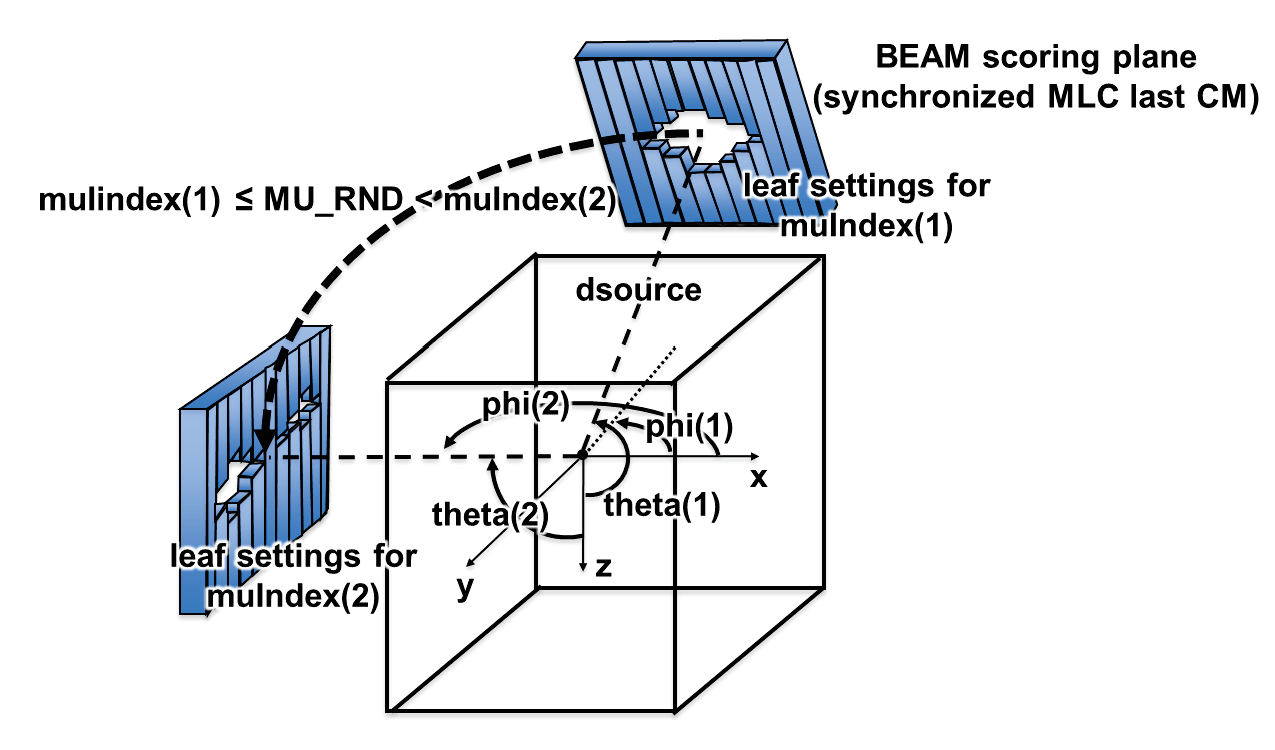
\includegraphics[width=18cm]{figures/src21_fig}
\caption{Source 21, including a synchronized CM, incident on a DOSXYZnrc phantom.  The figure indicates that the final CM in the treatment head
simulation is a synchronized MLC (SYNCVMLC, SYNCMLCE or SYNCHDMLC).  Two control points for the source plane, having different
{\tt muIndex}, {\tt theta} and {\tt phi}, are
indicated.  Different MLC leaf settings are also associated with the values of {\tt muIndex} (the user sets this up in
a file read by the synchronized CM).  Continuous motion of the source between ({\tt theta(1), phi(1)}) and ({\tt theta(2), phi(2)}), along
with dynamic motion of the MLC leaves,
is simulated for values of {\tt MU\_RND} with {\tt muIndex(1)}$\leq${\tt MU\_RND}$<${\tt muIndex(2)}.  Continous motion in
{\tt dource}, isocentre position ({\tt xiso, yiso, ziso}), and the angle of rotation of the source plane in the plane ({\tt phicol}) can
also be simulated.}
\label{src21_fig}
\end{center}
\end{figure}

\indexm{source 21!and non-EGSnrc shared library}
\subsubsection{Running the source through a non-EGSnrc shared library}

\indexm{the\_vcu\_code}\indexm{the\_vcu\_input\_file}
Using the inputs {\tt the\_vcu\_code} and {\tt the\_vcu\_input\_file} the user has the option to interpose another geometry
(usually an MLC) between the source plane and the DOSXYZnrc phantom.  In general, {\tt the\_vcu\_code} is a non-EGSnrc user
code.  Lobo and Popescu\cite{LP10} have used a version of the code particleDMLC\cite{Si02}, developed at Virginia Commonwealth University (hence ``vcu'' in the variable names), to place a simplified MLC simulation between the source and the phantom.

A detailed discussion of potential user codes for creating simplified MLCs is beyond the scope of this manual.  However,
a summary of the subroutines that must exist in {\tt the\_vcu\_code} and the parameters required to communicate
with DOSXYZnrc is given in the description of source 20 (Section~\ref{src20sect}) above.

Note that with source 21, {\tt dsource} always defines the Z-position, in the BEAM frame, of the source plane (scoring plane in the BEAM simulation), and
it is up to the user to ensure that the source is positioned correctly relative to the geometry
defined by {\tt the\_vcu\_code}.


\rfoot[{\sffamily \rightmark}]{{\sffamily \leftmark}}

\section{Other Source-Related Inputs}
\label{sec5}
After the inputs described above, there is another record input with
several other variables related mostly to the source.

\indexm{enflag}
\subsection {{\tt enflag}}
\label{enflag_sect}
The setting of {\tt enflag} determines whether the source is monoenergetic
or has an energy spectrum, or, if the source is a phase space file, whether
or not a dose component is to be calculated.
The possible settings of {\tt enflag} are:
\begin{description}
\item [~~~~= 0] (default) for a monoenergetic source ({\tt isource}=0,1,3,6).
\item [~~~~= 1] for an energy spectrum input ({\tt isource}=0,1,3,6).
\item [~~~~= 2] for a phase space source ({\tt isource}=2) or
full BEAM simulation source ({\tt isource}=9), no dose component
calculation.
\item [~~~~= 3] for a phase space source ({\tt isource}=2) or
full BEAM simulation source ({\tt isource}=9), dose component
calculation using a bit filter (see section~\ref{bitfiltersec} below).
\item [~~~~= 4] for a beam characterization model source ({\tt isource}=4).
\end{description}

\subsection {{\tt mode}}
\indexm{mode}
{\tt mode} only has meaning for a phase space source ({\tt isource}=2).
However, an explicit value for {\tt mode} must exist in the input file
for a full BEAM simulation source ({\tt isource}=9) or
beam characterization model source ({\tt isource}=4), since
{\tt isource}=4 and 9 make use of {\tt medsur}, {\tt dflag} and {\tt dsurround},
which occur after {\tt mode} on the same line.
The possible settings of {\tt mode} are:
\begin{description}
\item [~~~~= 0] (default) the phase space source does not contain
{\tt ZLAST} (for photons, Z of last site of interaction; for electrons,
Z where electron or its ancestor was set in motion by a photon) and, thus,
has 7 variables/record.
\item [~~~~= 2] the phase space source contains {\tt ZLAST} and, thus,
has 8 variables/record.
\end{description}

Note that DOSXYZnrc does not make use of {\tt ZLAST}, but it needs to know
whether {\tt ZLAST} is in the file or not so that the appropriate number
of variables/record can be read.  Thus, if a phase space file is only
going to be used as a source for a DOSXYZnrc calculation, you can save space
by leaving {\tt ZLAST} out of the file.  For more information
about {\tt ZLAST}, see the BEAMnrc Users Manual\cite{Ro09}.

\subsection {{\tt medsur}}
\indexm{medsur}
{\tt medsur} is the medium number for the region surrounding the phantom
as defined by {\tt dsurround}
(see below).  {\tt medsur} is only input for phase space, full BEAM
simulation or beam characterization
model sources ({\tt isource}=2, 4, 8 or 9).  The default setting of {\tt medsur}
is 0, indicating the
surrounding region is vacuum.  However, the user may set this to correspond
to any of the media that they have defined at the top of the DOSXYZnrc input file.
In many cases, the user may wish to fill this region with air and have particles
transported properly through air before reaching the phantom.

\subsection{{\tt dsurround} and {\tt dflag}}
\label{dflagsect}
\indexm{dsurround}
\indexm{dflag}

{\tt dsurround} and {\tt dflag} are required for phase space, full
BEAM simulation and
beam characterization model sources {\tt isource}=2, 4, 8, 9, 10, 20 or 21.
These inputs define the dimensions of the region surrounding the phantom
(ie filled with the medium defined by {\tt medsur}).  Note that
{\tt dsurround} is a 4-dimensional array
with {\tt dsurround(1)} occurring before {\tt dflag} on the input line
and {\tt dsurround(2...4)}, if required, occurring after {\tt dflag}.

The possible settings for {\tt dflag} and their relation to {\tt dsurround}
are as follows:

\begin{description}

\item [~~~~{\tt dflag}=0] (default) {\tt dsurround(1)} defines the thickness
if the surrounding region (in cm) on all sides of the phantom, and the user
need not
input values for {\tt dsurround(2...4)}.  {\tt dsurround(1)}
defaults to 50 cm if it is set $\leq$0.
\item [~~~~{\tt dflag}=1] means that {\tt dsurround(1)} defines the thickness of the
surrounding region in the $\pm$x directions, {\tt dsurround(2)} is the
thickness of the surrounding region in the $\pm$y directions, {\tt dsurround(3)}
is the thickness in the +z direction (bottom of the phantom)
and {\tt dsurround(4)} is the thickness
in the $-$z direction (top of the phantom).  {\tt dsurround(1...4)} default to 0.
\end{description}

Use of {\tt dflag}=1 with {\tt dsurround(1...4)} can save substantial amounts of
computing time if the user is only interested in the dose along a certain axis
or in a specific slice of a DOSXYZnrc phantom (see section~\ref{dsurround_section}
below).

\subsection{{\tt ein}}
\indexm{ein}

{\tt ein} is the kinetic energy of
a monoenergetic incident beam in MeV.  It defaults to 1.25 MeV if
{\tt ein} is set $\leq$ 0.  Note that {\tt ein} is only required if
{\tt isource}=0,1,3,6 and {\tt enflag}=0.

\subsection{{\tt FILNAM}}
\indexm{FILNAM}

{\tt FILNAM} is the file name (with extension) of:

\begin{description}
\item[incident beam energy spectrum] if {\tt isource}=0,1,3 or 6 and
{\tt enflag}=1.  In this case, {\tt FILNAM} has a specific format which
corresponds to the ensrc format used in the original EGSnrc system
\indexm{energy spectrum format}
(see {\tt \$HEN\_HOUSE/spectra} for a large number of
example spectra):

{\tt ENSRC.V5 File format\\
====================}
\begin{tabbing}
\= {\tt SPEC\_TITLE} \\
\> {\tt NENSRC, ENMIN, IMODE} \\
\> {\tt ENSRCD(I), SRCPDF(I) (I = 1 to NENSRC)} \\
\end{tabbing}
\vspace*{-5mm}
where:
\vspace*{-3mm}
\begin{description}
\item [~~~~{\tt SPEC\_TITLE}] is an 80-character spectrum title
\item [~~~~{\tt NENSRC}] = \# of energy bins in the spectrum histogram
\item [~~~~{\tt ENMIN}] = lower energy of first bin in MeV
\item [~~~~{\tt IMODE}] Set to 0 for histogram counts/bin; set to 1 for
counts/MeV
\item [~~~~{\tt ENSRCD(I)}] = upper energy of bin I in MeV
\item [~~~~{\tt SRCPDF(I)}] = probability of finding a particle in bin
I (SRCPDF
need not be normalized)
\end{description}

\item[phase space source:] if {\tt isource}=2 or 8 and {\tt enflag}=2 or 3.
See Section~\ref{source2sect} for more details.
\item[beam characterization model:] if {\tt isource}=4 and {\tt enflag}=4.
\indexm{the\_beam\_code}
\indexm{the\_input\_file}
\indexm{the\_pegs\_file}
\item[{\tt the\_beam\_code}, {\tt the\_input\_file}, {\tt the\_pegs\_file}:]
if {\tt isource}=9 or 10 and {\tt enflag}=2 or 3.  These are the names of the
BEAM accelerator code being used as a source, the input file for the BEAM
simulation, and the pegs data for the BEAM simulation respectively.  See
section~\ref{src9sect} for more details.
\end{description}

\subsection{{\tt IOUTSP}}
\indexm{IOUTSP}
{\tt IOUTSP} is only required with an incident energy spectrum ({\tt enflag}=1).  The
possible settings of {\tt IOUTSP} are:

\begin{description}
\item [~~~~= 0] (default) no output summary of incident energy spectrum
in {\tt .egslst}.
\item [~~~~= 1] output a summary of the incident energy spectrum to the
{\tt .egslst} file.
\end{description}

\section{Phase Space Sources}
\index{phase space sources}

The phase-space files output by BEAMnrc and used by DOSXYZnrc for sources 2 and 8 are
described in detail in section 7 of the BEAMnrc User's Manual.
\cite{Ro04a}.

The phase-space files are binary files  opened with ACCESS = 'direct' and
FORM = 'unformatted'.  Because they are binary files, and because there
are two common byte orders used for binary files by different systems
(eg PCs and DEC machines use one form and SUNs and SGIs use the other),
files written by one system may not be compatible with another system.
The utility {\tt readphsp} found on {\tt \$OMEGA\_HOME/progs/readphsp} can
convert files from one format to the other (see the description in the BEAMnrc
User's Manual. \cite{Ro04a}.)

There are also two types of phase-space files determined by how many
variables they contain.  The shorter format is
called '{\tt MODE0}' and  {\tt ZLAST} is not
scored and the longer format is
'{\tt MODE2}' when {\tt ZLAST} is present.  Since DOSXYZnrc makes no use of
the {\tt ZLAST} variable, it saves space to use {\tt MODE0} files for use with
DOSXYZnrc.  The '{\tt MODE0}' or '{\tt MODE2}'
designation appears in the first record of a phase-space file along
with the total number of particles contained in the file, the number
of photons, maximum energy of any particle in the file,
minimum energy of electrons, and minimum energy of
photons.

\indexm{phase space sources!negative energy marker}
\indexm{phase space sources!using old files}
\indexm{uncertainties}
\indexm{statistics}
Phase space files generated by BEAMnrc use negative
{\tt E} (energy) to mark the first particle scored by each new primary
history.  If the file is used as a source, then the negative {\tt E} marker
allows scored quantities (ie energy deposited) to be grouped according
to primary history.  This ensures that uncertainties estimated account
for the correlations between incident particles in a phase space
source~\cite{Wa02a}.  If an old phase space file without negative {\tt E} markers is used
as a source, then scored quantities will be grouped according to incident
particle instead of primary history.  DOSXYZnrc will then output a warning
that uncertainty may be underestimated because correlations between incident
particles could not be taken into account.  This is not a cause for concern,
because we have found~\cite{Wa02a} that in the cases we studied,
the underestimate is not significant.

When using a phase space source, if the entire phase space file is read
before the requested number of histories is run, then DOSXYZnrc restarts
the phase space file from the beginning.  For the reasons discussed in
section~\ref{nrcycl}, page~\pageref{nrcycl}, this is not a desirable
occurrence and one should strive to avoid this by using the recycling
feature (which also saves on reading time).

\index{IAEA-format phase space sources}
\label{iaeaphspsect}
\subsection{IAEA-format Phase Space Sources}

In addition to the standard BEAMnrc phase space files described
above, DOSXYZnrc can
also use IAEA-format phase space data as a source.  This allows the
user to make use of IAEA's online data base of accelerator phase space
data at:\\
\htmladdnormallink{www-nds.iaea.org/phsp/phsp.htmlx}{http://www-nds.iaea.org/phsp/phsp.htmlx}

\index{C++ compiler}
Note that this functionality requires that EGSnrc/DOSXYZnrc be installed on a machine
with a working C++ compiler.  This is detected automatically during
EGSnrc installation and, if a working C++ compiler is found, the library
of IAEA phase space handling routines is compiled.

\index{{\tt .IAEAheader}}
\index{{\tt .IAEAphsp}}
\index{IAEA phase space data! header file}
\index{IAEA phase space data! phase space data file}
Phase space data in IAEA format comprises both a header
(extension {\tt .IAEAheader}) file and a phase space data
(extension {\tt .IAEAphsp}) file.  When using IAEA phase space data as
a source, only the full name and directory path of the {\tt .IAEAphsp} file needs to be specified
(See Section~\ref{source2sect}).  The {\tt .IAEAheader} file is assumed to be
in the same directory.

Note that when IAEA phase space sources are used the incident Z-position of each particle
is available and is automatically read, either from the header file in the case of
planar phase space data (such as that scored by BEAMnrc), or from the phase space
data itself if it is scored in 3-D (such as that scored by DOSXYZnrc).  The ability to handle
3-D phase space data greatly enhances the flexibility of DOSXYZnrc and allows it to
use non-planar data supplied by manufacturers, such as that supplied by Varian for
their TrueBeam accelerators.  In addition, IAEA phase space files generated by BEAMnrc simulations
with synchronized component modules (CMs) and by DOSXYZnrc simulations using synchronized
sources (20 or 21) may include the fractional monitor unit ({\tt MU}) associated with each particle.
This is automatically read in and used by DOSXYZnrc's synchronized phase space source (source 20) allowing
synchronization between the DOSXYZnrc simulation and the upstream simulation that generated the phase
space file.  See Sections~\ref{src2iaeasect} and \ref{src20iaeasect} for more information.

Form more information on the format of IAEA phase space data, see the
BEAMnrc Manual and IAEA Report INDC(NDS)-0484\cite{CJ05}.

\section{Calculating Dose Components with DOSXYZnrc}
\label{bitfiltersec}
\subsection{Bit Settings}
\indexm{bit setting}

\indexm{LATCH}
The {\tt LATCH} variable, associated with each particle in a
BEAMnrc simulation, is a
32-bit variable used to track the particle's history.  It is discussed in
detail in the BEAMnrc User's Manual \cite{Ro04a}.

Each bit in {\tt LATCH} is designated as follows with bit 0 being the lowest value bit:
\begin{description}
\item [~~~~bit 0] Set to 1 if a photon is created by a bremsstrahlung event or an electron is created by a bremsstrahlung photon; 0
otherwise
\item [~~~~bits 1-23] Used to record the region where a particle has been and/or
has interacted. Note that the bit set for a region is determined by
{\tt IREGION\_TO\_BIT} (which is defined in the BEAMnrc simulation)
for that region.
\item [~~~~bits 24-28] Stores {\tt IREGION\_TO\_BIT} (as a binary number) of the
region in which a secondary particle
is created; if these bits are all 0, the particle is a primary
particle
\item [~~~~bits 29-30] Store the charge of a particle at the time {\tt LATCH} is output
\indexm{LATCH}
to a phase-space file.
\item [~~~~bit 31] Set to 1 if a particle has crossed a scoring plane
more than once when {\tt LATCH} is output to a phase-space file.
\indexm{LATCH}

\end{description}

For secondary particles, recording the {\tt IREGION\_TO\_BIT}'s of
the regions in which they were
created in bits 24-28 is equivalent to multiplying the {\tt IREGION\_TO\_BIT} by
2$^{24}$, or 16777216.  Thus, to retrieve {\tt IREGION\_TO\_BIT} of the region
of origin of a
secondary particle, the {\tt LATCH} value of the particle must be divided by
16777216 (i.e., taking the value {\tt INT(LATCH/16777216)}).
\indexm{LATCH}

When used with a phase space source, DOSXYZnrc has the
capability of selecting from the phase space file only those particles that
have user-specified bits (called a ``bit filter") set in their {\tt LATCH}
variables.
Thus, DOSXYZnrc will score only the dose component arising from these user-selected
particles.  For example, in the BEAMnrc simulation, bit 10 may be associated
with a square applicator, so any particle in the phase space file that has
been in the applicator will have bit 10 set in {\tt LATCH}.  When using
this phase space file as a source in DOSXYZnrc, the user may opt to use only
those particles that have bit 10 set, thus scoring the dose component from
particles that have been in the applicator.

In general, a dose component can be selected
according to what regions particles have passed through/interacted in,
whether the particle is a primary or secondary, if the particle is a
secondary then where it was created, and any combination of these.

\subsection{Input for Dose Component Calculations}

In order to enable dose component calculations with a phase space source
or full BEAM simulation source
({\tt isource}=2, 8 or 9),
the variable {\tt enflag} must be set to 3.  The user then specifies which
\indexm{enflag}
type of bit filter ({\tt I\_BIT\_FILTER}) to use.  Below is a description of the
4 types of bit filters available and the inputs associated with each.

\begin{description}
\indexm{I\_BIT\_FILTER}
\indexm{NBIT1}
\indexm{NBIT2}
\indexm{BIT}
\index{IREGION\_TO\_BIT}
\item [{\tt I\_BIT\_FILTER}=0] This is an inclusive/exclusive bit filter.  On the
same line as {\tt I\_BIT\_FILTER}, the user inputs the integers {\tt NBIT1} and
{\tt NBIT2}.  {\tt NBIT1} is the number of bits to include and {\tt NBIT2} is
the number of bits to exclude.  Restriction is that
0$\leq${\tt NBIT1}+{\tt NBIT2}$\leq$29.
Both {\tt NBIT1} and {\tt NBIT2} can be set to zero.  On the next line, the
user inputs {\tt BIT(I) (I=1,NBIT1)}, the bits to be included, and on
the following line \\ {\tt BIT(I) (I=NBIT1+1,NBIT1+NBIT2)}, the bits to
be excluded.  If any of the first set of {\tt NBIT1} bits are set and none
of the second set of {\tt NBIT2} bits are set in the particle's {\tt LATCH}
variable, the particle is used in the
simulation.

\item [{\tt I\_BIT\_FILTER}=1] This is an exclusive bit filter.  On the same line
as {\tt I\_BIT\_FILTER}, the user inputs the integer {\tt NBIT1}, the
number of bits to be excluded (0$\leq${\tt NBIT1}$\leq$29).  {\tt NBIT2} is
not relevant for this filter and is automatically set to 0.  On the
next line, the user inputs, {\tt BIT(I) (I=1,NBIT1)}, the bits to
be excluded.  If any of these {\tt NBIT1} bits are set in the particle's
{\tt LATCH} variable, the particle
is NOT used in the simulation.

\item [{\tt I\_BIT\_FILTER}=2] An inclusive region-of-origin filter.
The user inputs {\tt NBIT1} on the same line
as {\tt I\_BIT\_FILTER}, where {\tt NBIT1} is the number of regions of origin
to be included.  Since regions of origin are distinguished only by their
values of {\tt IREGION\_TO\_BIT}, {\tt NBIT1} can also be seen as the
number of distinct values of {\tt IREGION\_TO\_BIT} to be included. The
restriction on {\tt NBIT1} is 0$\leq${\tt NBIT1}$\leq$24.  {\tt NBIT2} is
not relevant for this filter and is automatically set to 0.  On the
next line, the user inputs {\tt IREGION\_TO\_BIT(I) (I=1,NBIT1)}, the
{\tt IREGION\_TO\_BIT} values of the {\tt NBIT1} regions of origin to
be included.  If the particle originated in any one of these {\tt NBIT1}
regions, then it will be used in the simulation.  Primary particles will be included if
{\tt IREGION\_TO\_BIT=0} is one of the {\tt NBIT1} values of
{\tt IREGION\_TO\_BIT} to include.

\item [{\tt I\_BIT\_FILTER}=3] An exclusive region-of-origin filter.
The user inputs {\tt NBIT1} (0$\leq${\tt NBIT1}$\leq$24), the number of
regions of origin to be excluded, on the same line as {\tt I\_BIT\_FILTER} and
ignores {\tt NBIT2}, since it is not relevant for this filter.  On the
next line the user inputs {\tt IREGION\_TO\_BIT(I) (I=1,NBIT1)}, the
{\tt IREGION\_TO\_BIT} values of the regions of origin to be excluded.
If a particle originated in any one of these regions, then it is NOT
used in the simulation.  Note that primary particles will be excluded if
{\tt IREGION\_TO\_BIT=0} is one of the {\tt NBIT1} values of
{\tt IREGION\_TO\_BIT} to exclude.

\end{description}

Note that since only one bit filter can be input per simulation, only one
dose component may be calculated at a time using DOSXYZnrc.  This is because
of the large memory requirements for the dose scoring arrays.

\section{Other Input Variables}

This section provides descriptions of main DOSXYZnrc input variables not
covered above.

\vspace*{-0.5cm}
\subsection{{\tt IPHANT}}
\label{iphantsect}
\indexm{IPHANT}

If {\tt IPHANT} is set to 1, DOSXYZnrc outputs phantom data to
a {\tt .egsphant} file.  This file has the same format as the
{\tt .egsphant} file that {\tt ctcreate} outputs for CT data
(see section~\ref{egsphantsect}) and can be read by
{\tt dosxyz\_show}\cite{Ka98},
along with the {\tt .3ddose} dose output file to display isodose contours in
the phantom.  Note that this option is redundant (and, therefore, unavailable)
when using a CT phantom because it is an input file from ctcreate).

\subsection{{\tt MAX20}}
\indexm{MAX20}
\label{MAX20description}

When {\tt MAX20} is set to 1, a summary of the maximum 20 doses in the
phantom is output to the screen (log file) and list file.  This summary
includes an output of the 20 maximum doses with their fractional
uncertainties and coordinates, the average of the 20 maximum doses, the average
fractional uncertainty of these doses (not the uncertainty of the average), the
average fractional uncertainties of all doses $>$ 50\% of the maximum dose,
and the average absolute uncertainty of all doses $>$ 50\% of the maximum dose
as a fraction of the maximum dose.

When not in CT phantom mode, {\tt MAX20} is the last variable on the line(s)
specifying the regions for which dose will be output (ie record 9).  If
{\tt MAX20} is set to 1 on ANY ONE of these lines (including the line of
zeros indicating the end of this record) then the summary of the 20 maximum
doses will be output.

In CT phantom mode, {\tt MAX20} is input
\indexm{MAX20} on the same line as {\tt zeroairdose} and {\tt doseprint}.

This option is useful for timing/efficiency studies.
\subsection{{\tt zeroairdose}}
\indexm{zeroairdose}
\label{zeroairdose}

{\tt zeroairdose} is only used in CT phantom mode.
Setting {\tt zeroairdose} to 1 will set all dose estimates in
voxels with density $<$ 0.044 g/cm$^3$ to zero in the {\tt .3ddose}
\indexm{.3ddose}
\indexm{files!.3ddose}
file.  This has the effect of zeroing dose in voxels filled with air
(see the default CT ramp in Figure~\ref{fig_ct02}--note that ``AIR''
has a density ranging from 0.001-0.044 g/cm$^3$).
Air dose will not be zeroed in the {\tt .egslst} file, this file will
continue to report the precise estimated dose.  {\tt zeroairdose} serves
as a dose visualisation parameter for CT phantom simulations, since, in general, the user is only interested
in seeing the dose within the patient, not in the surrounding air.

\subsection{{\tt doseprint}}
\indexm{doseprint}

This input parameter is also only used in CT phantom mode.

{\tt doseprint} is set to 1 if the user wants a full output of doses in
all voxels of the CT phantom in the {\tt .egslst} file.  Since, in CT
phantom cases, the user is usually not interested in this output and, owing
to the large number of voxels in a CT phantom, it can make the {\tt .egslst}
exceptionally large, the default is to suppress this output (ie set
{\tt doseprint} to 0).

\subsection{{\tt NCASE}}
\indexm{NCASE}

{\tt NCASE} is the number of histories to run in a simulation.  Minimum
value is 100.  Default is 100 if {\tt NCASE} is set $<$ 100.  The number
of histories per output batch is equal to {\tt NCASE}/({\tt \$NBATCH}),
where {\tt \$NBATCH} is currently set to 10.

\subsection{{\tt IWATCH}}
\indexm{IWATCH}

{\tt IWATCH} controls output to the screen (interactive run) or to the
{\tt .egslog} file (batch run) during beam execution.  The possible settings
are:
\begin{description}
\item [~~~~= 0] (default) On completion of each batch, outputs information about the
batch (eg elapsed time, CPU time, elapsed/CPU time, random number used
to begin batch, \# of random seeds used in the batch, total number of
histories run up to and including the current batch, the total number of
particles scored in the first phase-space file)

\item [~~~~= 1] Outputs same information as 0 plus, after every particle
interaction, outputs complete information about the particle(s)
involved (eg interaction type, particle type, position of particle on
stack, particle energy, X-Y-Z position of particle, U-V-W direction
cosines, {\tt LATCH} value of particle, region \# of particle); also informs
\indexm{LATCH}
user when a particle is being discarded, when a particle is passing from
one CM to another

\item [~~~~= 2] Similar to 1 but with complete particle information output at
every step; also outputs total dose in a region whenever energy is
deposited there

\item [~~~~= 3] Similar to 2 but with particle and dose information output
whenever dose is deposited.

\item [~~~~= 4] Outputs same information as 0 plus {\tt .egsgph} and {\tt
.egsgeom} files for graphical representation of the accelerator and
particle paths using {\tt EGS\_Windows.}
\indexm{.egsgph}
\indexm{.egsgeom}
\indexm{files!.egsgph}
\indexm{files!.egsgeom}
\end{description}

\subsection{{\tt TIMMAX}}
\indexm{TIMMAX}

{\tt TIMMAX} is the maximum CPU time in hours allowed for a simulation.
{\tt TIMMAX} defaults to 0.99 hrs if it is set = 0.  However, this time-restriction function is not activated in the current version of DOSXYZnrc except to
print a warning as it starts a batch which will exceed this limit.


\subsection{{\tt INSEED1, INSEED2}}
\indexm{INSEED}
\indexm{RANMAR}
\indexm{RANLUX}
\indexm{random number generator}
\indexm{random number seeds/pointers}

These are random number seeds used to initialize the
RANMAR\cite{MZ91,Ma90a} or RANLUX\cite{La94,Ja94}
random number generator.  Within DOSXYZnrc,
{\tt INSEED1} is limited
to the range\\ 0$<${\tt INSEED1}$\leq$31328
(defaults to 1802), and {\tt INSEED2} has
the range 0$<${\tt INSEED2}$\leq$30081 (defaults to 9373).  These
ranges/defaults are designed for RANMAR (the default random number generator),
however, if
you are using RANLUX then {\tt INSEED1} is the ``luxury level"
of the random number generator and must be in the range
0$<${\tt INSEED1}$\leq$4, otherwise, it will automatically be set to the
default luxury level of 1 (Note: this means that the DOSXYZnrc default value
for {\tt INSEED1} of 1802 will ultimately get reset to 1 by RANLUX).

Note that \verb+INSEED1+ and \verb+INSEED2+ are only used to initialize
the random number generator, and, during a simulation, they no longer
reflect the values of the seeds that are actually used to generate
the random numbers.
When resuming
({\tt IRESUME} = 1), the state of the random number generator at the end
of the previous run is read from the {\tt .egsdat} file and is used when the
simulation resumes.
Thus, a resumed run with a total of
10000+10000 histories should generate results identical to a single run
of the same simulation with 20000 histories.  Also note that
when running parallel jobs
with DOSXYZnrc (see section~\ref{parallelcalc}), {\tt INSEED2} must have
a different value for each of the individual jobs that make up the simulation.
This is taken care of automatically if you use DOSXYZnrc's built-in
parallel processing functionality.

\index{random number generator! switching from RANMAR to RANLUX}
In order to switch from the RANMAR random number generator to RANLUX in
DOSXYZnrc, go into {\tt \$EGS\_HOME/dosxyznrc/Makefile} and
change the line:
\begin{verbatim}
RANDOM = $(EGS_SOURCEDIR)ranmar
\end{verbatim}
to:
\begin{verbatim}
RANDOM = $(EGS_SOURCEDIR)ranlux
\end{verbatim}
Then recompile DOSXYZnrc.

\subsection{{\tt BEAM\_SIZE}}
\indexm{BEAM\_SIZE}

{\tt BEAM\_SIZE} allows the user to control the maximum beam size for phase space sources (sources 2,
8, 20), BEAM simulations sources (souces 9, 10, 21) and the beam model source (source 4).
{\tt BEAM\_SIZE} is the side of a square field in cm. The default value for {\tt BEAM\_SIZE} is 100 cm.
Particles are discarded immediately if they are outside the
square defined by {\tt BEAM\_SIZE} centred on the beam axis in the source scoring plane.

One should be careful with the use of this parameter because particles outside
the specified field (defined by {\tt BEAM\_SIZE)} may have some effects on the dose
distributions calculated and therefore the results may be biased with the use
of {\tt BEAM\_SIZE} smaller than the field size of the original phase-space data. It
should also be noted that this parameter cannot be used as a beam defining tool,
such as a collimator,
because in reality particles outside of the inner opening of any beam confining
components may interact with and be scattered by the components,  resulting in
an increase of the particles within the specified field.

\subsection{{\tt ISMOOTH}}
\label{ismooth}
\indexm{ISMOOTH}

\indexm{re-use of phase space}
When phase-space data are used DOSXYZnrc will re-use the phase-space particles if
\indexm{phase-space input}
the number of histories required by the user is greater than the number of
particles stored in the phase-space file. Clearly, the dose distributions
obtained with more histories have smaller statistical uncertainties.
Although some histories may start with the same incident phase-space, the
particle trajectories will be different because different random numbers will
be used in the simulations in the phantom, resulting in different dose
distributions. However, surface doses are mainly affected by the electron
fluence distribution and therefore would not be improved by re-using the
phase-space particles if the data file contains too few particles
(i.e., the calculated doses
would have small statistical uncertainties but large systematic uncertainties).

In order to reduce the systematic uncertainties due to a small data set,
DOSXYZnrc can re-distribute the phase-space particles {\bf as long as the
simulated linear accelerator geometry is symmetric,  and the treatment
field is centred on the beam axis}. Currently, DOSXYZnrc is allowed to move a
particle  to 3 symmetrical positions (each with modified direction
cosines). This process is accurate as long as the phase space file is
symmetric with respect to the x-axis and also with respect to the
y-axis.  Suppose a particle is at (x,y) with (u,v) the 3 new positions
are
\begin{center}
(-x,y) with (-u,v), \\
(x,-y) with (u,-v), \\
(-x,-y) with (-u,-v)
\end{center}
%%Dave commented the following out since even after corrections, he
%is not at all convinced it is right.
%If further, their is a square symmetry (eg if no jaws are included in the
%simulated linear accelerator geometry or they are all on the same level),
%one can further move the particle
%to 4 other positions (one needs to modify DOSXYZnrc in order to do so), i.e.,
%
%\begin{center}
%
%(x,y) with (-u,-v),
%
%(-x,y) with (u,-v),
%
%(x,-y) with (-u,v),
%
%(-x,-y) with (u,v)
%\end{center}
A user has two options for {\tt ISMOOTH}:
\indexm{ISMOOTH}
\begin{description}
\item [~~~~= 1] DOSXYZnrc re-distributes the phase-space particles when they are used more than once.


\item [~~~~= 0] (default) DOSXYZnrc re-uses the phase-space particles without changing the particle positions

\end{description}
\indexm{re-use of phase space}

See also section~\ref{nrcycl} which discusses recycling phase space data.

\subsection{{\tt NRCYCL}}
\label{nrcycl}
\indexm{NRCYCL}
\indexm{phase space source!recycle}

{\tt NRCYCL} is an essential input when using a phase space source. It
determines the number of times that each particle from a phase space
source is recycled ({\em  ie}, reused each time it is read).
If {\tt NRCYCL}$>$0, then
each source particle is used a total of {\tt NRCYCL} + 1 times
before moving on to the next particle in the source.
When phase space data is sparse, then particles must be re-used to obtain
adequate statistics.  In addition to recycling, particles may also
be re-used whenever a phase space source is restarted
(happens automatically when the simulation has reached
the end of the source).  Restarting is not recommended, however,
because it may lead to underestimates of the uncertainty in the
final results~\cite{Wa02a}.  We recommend setting {\tt NRCYCL} to a value
that will ensure that the entire phase space source gets sampled (ie
the simulation uses almost all the particles in the source) but
prevents the source from being restarted.

If you are unsure of
the correct value of {\tt NRCYCL} to use, then
run with {\tt NRCYCL}=0 and DOSXYZnrc will automatically calculate
a value of {\tt NRCYCL} based on the number of histories and
the number of particles (with appropriate charge) in the phase space source.
There is a possibility
that, even with the automatically calculated value of {\tt NRCYCL},
the phase space source will restart.  This may be due to particles
that have been rejected because they missed the geometry, were multiple
passers and/or were beyond the beam field defined by {\tt BEAM\_SIZE}) or
else the algorithm for calculating {\tt NRCYCL} may have determined that
setting {\tt NRCYCL}$>$ 0 will result in the phase space source not being
sampled adequately.
If the
source has only been restarted once and only a small fraction of it
has been covered on the second pass, this is not likely to have a significant
impact on the estimated uncertainties.  However, if a large portion of the
source is covered on the second pass, or if it is restarted more than once,
we recommend re-running the simulation with a new value of
{\tt NRCYCL} calculated as:
\begin{eqnarray}
\label{nrcycleqn}
{\tt
NRCYCL}=
\frac{{\tt NCASE}}{\left({\tt NPHSP - (NSMISS/NRCYCL}_{prev}) - {\tt NOUTSIDE - NRJCT - NDBSRJCT}\right)}-1
\end{eqnarray}
where {\tt NCASE} is the number of incident histories, {\tt NPHSP} is the
total number of particles in the phase space file, {\tt NSMISS} is
the number of particles that missed the geometry in the previous run,
{\tt NRCYCL$_{prev}$} is the setting of {\tt NRCYCL} in the previous run,
{\tt NOUTSIDE} is the number of particles rejected because they were
outside the field defined by {\tt BEAM\_SIZE} in the previous run,
{\tt NRJCT} is the number of particles rejected because they were
multiple passers in the previous run, and {\tt NDBSRJCT} is the number of
photons rejected because they fall outside the directional bremsstrahlung
splitting (DBS) field radius at the SSD (only if DBS was used in the BEAM
simulation that generated this source AND the user has opted to reject
these photons--see section~\ref{source2sect} for more information about
this).  Note that {\tt NPHSP}, {\tt NSMISS}, {\tt NOUTSIDE},
{\tt NRJCT} and {\tt NDBSRJCT} are all available from the {\tt .egslst} file of the previous run.
Always round your calculated value of {\tt NRCYCL} up to the nearest integer.
\indexm{DBS}
\indexm{NRCYCL}

{\tt NRCYCL} is not automatically calculated if you are only using the
positrons in the phase space source or if you are selecting a sub-set of
the phase space source based on {\tt LATCH} settings.  In these cases,
the information required for an a-priori calculation of {\tt NRCYCL}
is not available in the header of the phase space source.
We recommend setting {\tt NRCYCL} manually to a ``best guess" value.  Then,
if the source restarts, calculate {\tt NRCYCL} using Equation~\ref{nrcycleqn}
where {\tt NRJCT} includes the number of particles rejected because they
were multiple passers, the number of particles rejected because they were
the wrong charge and the number of particles rejected because they did not
have the right {\tt LATCH} setting.

If the phase space source is stored on a remote disk, then using
{\tt NRCYCL} to avoid restarting a phase space source also has
the beneficial effect of reducing network traffic
because it reduces the number of times that a phase space
source is accessed during a run (particle data is stored in temporary
variables during recycling, not re-read from the source).  Repeated
accessing of a phase space source on a remote disk can slow a simulation
down considerably.

{\tt NRCYCL} is compatible with {\tt ISMOOTH} (see section~\ref{ismooth}).
So if {\tt ISMOOTH}=1, then,
during the recycling loop, the initial position and direction cosines of
the particle are shifted according to the scheme outlined in the
{\tt ISMOOTH} subsection above.
\indexm{ISMOOTH}
\indexm{NRCYCL}

Note that the total number of histories is
always limited by {\tt NCASE}.  For example, if the
phase space source has 1000 suitable particles and the user sets {\tt NRCYCL}=9
(so each particle will be used a total of 10 times), but only sets
{\tt NCASE}=5000, then the simulation will only have a chance to use (and
recycle) the first 500 particles before the simulation stops.  In order to
go through the entire phase space source, the user would have to set
{\tt NCASE}=10000.  If {\tt NCASE}$>$10000 then the phase space source
would be restarted at least once during the run.  After restarting, particle
recycling continues as before.

\subsection{{\tt IRESUME}}
\label{iresumesect}
\indexm{IRESUME}
\indexm{resuming}

\indexm{.egsdat}
The possible settings of {\tt IRESUME} are:
\begin{description}
\item [~~~~= 0] (default) DOSXYZnrc initiates a new run, deleting all of the output
files ({\tt .egslog,} {\tt .egslst}, {\tt .egsdat}, \etc) if present
\item [~~~~= 1] Resume a previous run; DOSXYZnrc opens the
{\tt .egsdat} from the previous run and reads:
\begin{enumerate}
\item $\sum_{i=1}^{nhist}edep_i$ and $\sum_{i=1}^{nhist}edep_i^2$ for
all voxels, where {\tt edep$_i$} is energy deposited by primary (non-phase space)
history i
and {\tt nhist} is the number of primary histories in the previous run.
\item number of histories and number of primary histories from the previous run
\item the time taken by the previous run
\item the state of the random number generator at the end of the
previous run
\item other data relating to particle fluence in previous run, number of
electron steps, number of particles rejected from phase space source (if
applicable), etc.
\end{enumerate}
After the current run is complete, dose and
uncertainties are calculated using data from the current run and from
the previous run~\cite{Wa02a}.  Note that the
number of histories to run and the total CPU time allowed for the
simulation do not include the histories and CPU time from the previous run.
Also note that, currently, although a resumed simulation with, for example
100000+100000 histories will have identical dose results to a one-off
simulation
with 200000 histories, the uncertainty estimates on the doses may not be
the same.  We are currently investigating why this is so.
\item [~~~~= 2] DOSXYZnrc creates the {\tt .egsinp} file and then exits without
running the simulation
\item [~~~~= 3] DOSXYZnrc opens the {\tt .egsdat} file from a previous run,
reads the data enumerated above and calculates doses and uncertainties;
no simulation is run.
\indexm{.pardose}
\item [~~~~= 4] DOSXYZnrc recombines the binary {\tt .pardose} files from
parallel jobs and creates {\tt .egslst} and {\tt .3ddose} output
files from the recombined data (see section~\ref{parallelcalc} for
more about parallel jobs).
\end{description}

\subsection{{\tt IDAT}}
\label{idatsect}
\indexm{IDAT}
\indexm{files!.egsdat}
\indexm{.egsdat}

The possible settings of the variable {\tt IDAT} are:
\begin{description}
\item [~~~~= 0] (default) DOSXYZnrc outputs {\tt .egsdat} file with
resume data after every batch.
\item [~~~~= 1] DOSXYZnrc does not output a {\tt .egsdat} file at all.
\item [~~~~= 2] DOSXYZnrc outputs a {\tt .egsdat} with resume data only at
the end of the entire run.
\end{description}
For large phantoms, writing this file will take a lot of time. For
production runs use 2 usually.

\subsection{{\tt IREJECT}}
\indexm{IREJECT}

{\tt IREJECT} is a switch for turning on charged particle range
rejection.  Range rejection can save simulation time by terminating
\indexm{range rejection}
particle histories immediately if they cannot reach
the boundary of the current voxel with energy $>$ {\tt ECUT} and their
current energy is less than {\tt ESAVE\_GLOBAL}. This is the same as the
{\tt IREJECT\_GLOBAL} = 2 option in the BEAMnrc code as discussed in the
BEAMnrc User's Manual \cite{Ro04a}.
\indexm{range rejection}
\indexm{ESAVE\_GLOBAL}
\indexm{ECUT}

The possible settings of {\tt IREJECT} are:
\indexm{IREJECT}

\begin{description}
\item [~~~~= 0] (default) DOSXYZnrc will not perform charged particle range
rejection.
\item [~~~~= 1] DOSXYZnrc will immediately terminate the history of a
charged particle and deposit its remaining energy in the current voxel
if its energy is $<$ {\tt ESAVE\_GLOBAL} (see description
in next section) and if it cannot reach the nearest voxel boundary with
an energy $>$ {\tt ECUT}.
\indexm{ESAVE\_GLOBAL}
\indexm{ECUT}
\end{description}

It is found that for 5~mm$^3$ voxels, range rejection can save 10 to 17\%
on computing time but for smaller voxels it saves less time (3 to 4\%
for 2.5~mm$^3$ voxels).  For non-CT phantoms where one can arrange to
have at least some of the voxels quite large, the savings will be
correspondingly larger, especially using the dsurround option
(see section~\ref{dsurround_section}).

Similar to BEAMnrc, range to {\tt ECUT} is determined by subtracting
the range from {\tt ECUT} to {\tt AE} (determined using EGSnrc macros and
EGSnrc-calculated tables of range to {\tt AE} as a function of particle
energy) from the particle's {\tt range} to {\tt AE} (calculated in EGSnrc)
at every charged particle step.  Rejection of particles based on
range to {\tt ECUT} is performed by a DOSXYZnrc macro and
not by the EGSnrc's built-in range rejection macro.  This
is because the EGSnrc range rejection is based on range to
{\tt AE} and not {\tt ECUT}.
\indexm{range rejection}

\subsection{{\tt ESAVE\_GLOBAL}}
\indexm{ESAVE\_GLOBAL}

{\tt ESAVE\_GLOBAL} is the maximum energy (in MeV) for which range rejection
\indexm{range rejection}
calculations will be performed (ie a particle cannot be rejected if its
energy is $\geq$ {\tt ESAVE\_GLOBAL}).  This option is to prevent
termination of high-energy electrons which are likely to generate
bremsstrahlung.
\indexm{range rejection}

\subsection{{\tt n\_split}}
\label{nsplitsect}
\indexm{n\_split}
\indexm{photon splitting}

{\tt n\_split} is used to control DOSXYZnrc's photon splitting option.
If {\tt n\_split} is set $>$ 1 all photons are split
into {\tt n\_split} photons, each with a weight equal to
$\frac{1}{{\tt n\_split}}$ times the weight of the original photon.  For each
photon, i, where i=1,2,...,{\tt n\_split}:
\begin{itemize}
\item The mean free path to its next interaction, $DPMFP_i$, given by
\begin{equation}
DPMFP_i=-{\tt ln}\left(1-\frac{\eta+i-1}{{\tt n\_split}}\right)
\end{equation}
where $\eta$ is a random number, chosen once for all {\tt n\_split} photons.
\item At the interaction site, each photon i produces charged particles and/or
scattered
photons.  Russian roulette is played on all scattered photons with a
survival probability of $\frac{1}{{\tt n\_split}}$.  Surviving photons
have their weight increased by {\tt n\_split} so that their weight is equal
to the weight of the
original photon before splitting.  All charged particles survive with weight equal
to $\frac{1}{{\tt n\_split}}$ times the original weight.
\item If these charged particles undergo radiative events (bremsstrahlung,
  annihilation, annihilation at rest), Russian roulette is played on the
  resultant photons with a survival probability of $\frac{1}{{\tt n\_split}}$.  Again,
  surviving photons have their weight increased by {\tt n\_split} so that their
  weight is equal to the weight of the original photon before splitting.
\item Photons whose weight has been restored to the original weight are
  subject to splitting again.
\end{itemize}

Photon splitting has the potential to increase the efficiency of a dose
calculation more than photon interaction forcing.  A good rule of thumb for
the setting of {\tt n\_split} is:
\begin{equation}
{\tt n\_split}>=\frac{N}{1-e^{-\lambda}}
\end{equation}
where $\lambda$ is approximately equal to the number of photon mean free paths
in the geometry of interest and {\tt N} $\geq$ 5.  This will increase the
number of primary interactions per incident photon by approximately {\tt N},
so reduce {\tt NCASE} by a factor of {\tt N}.

\indexm{photon splitting!with phase space sources}
\indexm{photon splitting!with BEAMnrc sim. sources}
It has recently been shown\cite{KW06} that the use of photon splitting
with a phase space source (Section~\ref{source2sect}) or BEAMnrc
simulation source (Section~\ref{src9sect}) can increase
the efficiency of dose calculations in simulated photon beams by
a factor of up to 6.5 (depending on beam energy, field size and phantom
voxel size).  Moreover, the optimum efficiency ({\em i.e.} at the
optimum value of {\tt n\_split}) with a BEAMnrc simulation
source is only 3--13\% lower than that with the corresponding
phase space source, potentially eliminating the need to store
phase space data.  Thus, it is highly-recommended that you use photon
splitting to increase the efficiency of photon beam dose calculations.
The optimum setting of {\tt n\_split} for phase space and BEAMnrc simulation
sources depends
on incident beam energy, field size and phantom voxel size.  For
BEAMnrc simulation sources, splitting numbers of
40 ($0.25\times0.25\times0.25$ cm$^3$ voxels) or 32
($0.5\times0.5\times0.5$ cm$^3$ voxels) should give efficiencies close
to the optimum, and for phase space sources, splitting numbers of
32 ($0.25\times0.25\times0.25$ cm$^3$ voxels) or
24 ($0.5\times0.5\times0.5$ cm$^3$ voxels) will be close to the optimum.
Note that these settings of {\tt n\_split} are higher than those
calculated using the rule of thumb given in the paragraph
above.  This is because much of the efficiency improvement is due to the
fact that {\tt n\_split} reduces the number of source particles required,
thus reducing the CPU time spent generating the source particles
(transport through the jaws in the case of a phase space source,
performing an entire treatment head simulation in the case of a BEAMnrc
simulation source), whereas the rule of thumb is based on the efficiency
improvement being solely due to the efficiency inherent in the
splitting algorithm itself.

\indexm{e\_split}
When {\tt n\_split} is used with a phase space or BEAMnrc simulation
source, then contaminant electrons may compromise dose statistics because
they are fewer and will have a higher weight than the split photons
(which contribute most of the dose).  To avoid this, the phase space
sources ({\tt isource}=2,8) and the BEAMnrc simulation source
({\tt isource}=9) have an input, {\tt e\_split}, which can be used to
split charged particles {\tt e\_split} times as soon as they enter
the phantom geometry.  The weight of the particle is reduced by
1/{\tt e\_split}.  To maximize efficiency, it is recommended that you
set {\tt e\_split}={\tt n\_split} if you
are using photon splitting with a phase space or BEAMnrc simulation source.
For more information about {\tt e\_split} see Sections~\ref{source2sect}
and~\ref{src9sect}.

\subsection{{\tt ihowfarless}}
\label{howfarlesssect}
\indexm{ihowfarless}
\indexm{``HOWFARLESS'' option}

If {\tt ihowfarless} is set to 1, then DOSXYZnrc uses the ``HOWFARLESS''
algorithm for transport in the phantom.

The ``HOWFARLESS'' algorithm is used to significantly increase the
efficiency of dose calculations in a homogeneous phantom.  When the option
is used, the {\tt HOWFAR} and {\tt HOWNEAR} subroutines in DOSXYZnrc only
consider the extreme outer boundaries of the phantom when calculating
the distance along the particle trajectory to the next region boundary
and the perpendicular distance
to the nearest region boundary respectively.  This eliminates the need
to stop at voxel boundaries and, hence, speeds up charged particle
transport considerably.  For the purposes of dose deposition, the
total curved charged particle step is approximated by two straight-line
steps joined at a hinge point.  The straight-line steps can be calculated
based on either the known initial position/direction of the particle
or its known final position/direction.  As coded, the ``HOWFARLESS''
algorithm uses a 1:1 mixture of step approximations based
on the initial position/direction and approximations based on the
final position/direction.  This has been found to give accurate dose
results over all energies and maximum allowed step lengths
(input variable {\tt SMAX}, see paragraph below).

When the ``HOWFARLESS'' option is used, the limitations on step
length within the phantom become the maximum allowable charged particle step length,
{\tt SMAX} (see Section~\ref{smaxsect}), and the maximum fractional
energy loss per electron step, {\tt ESTEPE} (see Section~\ref{estepesect}).
It is recommended that you leave {\tt SMAX} at its default
value (5 cm if you are using the {\tt PRESTA-I} boundary crossing
algorithm or electron step algorithm, 1e10 cm if you are using
the {\tt EXACT} boundary crossing algorithm and the {\tt PRESTA-II}
electron step algorithm).  At most beam energies, this will ensure
that step length is only limited by {\tt ESTEPE}, which it is not
recommended that you change.

The efficiency gained using the ``HOWFARLESS'' algorithm depends on
the source type, energy, field size, phantom voxel size, and the
boundary crossing algorithm (BCA) used.  For a photon beam from a
BEAMnrc-simulated linac (using either a phase space source or
full BEAMnrc simulation source),
use of ``HOWFARLESS'' increases the efficiency by $\sim$30\% when the
{\tt PRESTA-I} BCA is used, and by a factor of 2.5-3.5 when the more
accurate (but much slower) {\tt EXACT} BCA is used.  In the case of
a simple photon beam source ({\em e.g.} a parallel beam simulated using
{\tt isource}=1) with an energy spectrum, the efficiency gain with
``HOWFARLESS'' is a factor of 1.5-2.5 with the {\tt PRESTA-I} BCA
and a factor of 5-9 with the {\tt EXACT} BCA.  The highest efficiency
gains occur in monoenergetic electron beams, where ``HOWFARLESS''
increases the efficiency by a factor of 3-4 with the {\tt PRESTA-I}
BCA and 8-14 with the {\tt EXACT} BCA.  Efficiency gains are much
greater with the {\tt EXACT} BCA because calculations with standard
HOWFAR use the BCA at every voxel boundary, while ``HOWFARLESS''
calculations use the BCA only at the extreme outer boundaries of the phantom.
Thus, the standard calculation becomes much slower when the BCA is
switched from {\tt PRESTA-I} to {\tt EXACT}, while the speed of
the ``HOWFARLESS'' calculation does not decrease appreciably.  For
more information about BCA's see Section~\ref{bcasect}.

Use of ``HOWFARLESS'' is recommended in all homogeneous phantom calculations,
such as those used for beam commissioning.  More information about
this option can be found in the ``HOWFARLESS'' paper by
Walters and Kawrakow\cite{WK06}.

\subsection{{\tt i\_phsp\_out}}
\label{phspoutsect}
\indexm{i\_phsp\_out}
\indexm{writing phase space data}

If {\tt i\_phsp\_out} is set to 1 or 2, DOSXYZnrc outputs phase space data in IAEA format
for particles leaving the phantom geometry.  The phase space data is in 3-D, meaning
that it includes
the (X,Y,Z) position for each particle.  If {\tt i\_phsp\_out}=1, then the particle positions
are in the DOSXYZnrc coordinate system, and if {\tt i\_phsp\_out}=2, the particle positions
are transformed into the BEAMnrc, or source, coordinate system.  Note that phase space
output requires the existence of a region surrounding the phantom geometry and, thus, is limited
to phase space sources (source no.'s 2, 8, 20), BEAMnrc simulation sources (source no.'s 9, 10, 21)
and the multiple source model (source no. 4), all of which require the input of
\indexm{dflag}\indexm{dsurround}
{\tt dflag} and {\tt dsurround} to define the dimensions and medium of a surrounding region
(see Section~\ref{dflagsect}).

\indexm{i\_muidx\_out}
If phase space data is output when source 20 (synchronized phase space source) or 21 (synchronized BEAM simulation
source) is used then, through the {\tt i\_muidx\_out} input for those sources (see Sections~\ref{src20sect} and~\ref{src21sect}),
the user has the option to also include the fractional monitor unit index, {\tt MU}, associated with the particle
in the output phase space data.  Thus, the data includes a time dimension and is considered 4-D. Scoring
4-D data allows simulations downstream of the DOSXYZnrc simulation--{\it e.g.} BEAMnrc simulations with
synchronized component modules or further DOSXYZnrc simulations with synchronized sources--that use the
phase space data as a source to be synchronized with the DOSXYZnrc simulation that generated the phase space
file.

Since it includes the Z-position of each particle, the size of an IAEA phase space file written by
DOSXYZnrc may be slightly larger than that written by BEAMnrc, with the minimum record size (bytes/particle) for
DOSXYZnrc being 33 bytes while that for BEAMnrc is 29 bytes.  If {\tt MU} is included in the phase space
data, then the record size increases to 37 bytes.  Note that DOSXYZnrc does not have an option to
\indexm{ZLAST}
include {\tt ZLAST} (Z position of last site of photon interaction or creation of secondary charged particle) in
the phase space output.

\indexm{phase space file output!naming scheme}
Unlike BEAMnrc, DOSXYZnrc does not have the possibility of defining multiple phase space scoring planes.
Thus, the naming scheme for phase space space files output by DOSXYZnrc does not include the scoring plane
number, and the files are simply named {\tt inputfile.IAEAheader} (header file) and {\tt inputfile.IAEAphsp}
(phase space data).

The default directory for phase space output is {\tt \$EGS\_HOME/dosxyznrc} ({\it i.e.} the user code directory).
The user can change the phase space output directory by editing the file\\
 {\tt \$EGS\_HOME/dosxyznrc/dosxyznrc\_user\_macros.mortran}, changing the macro\\ {\tt \$DIRECTORY-FOR-PHSP} to the name of the desired output directory (include
the full path), and then recompiling DOSXYZnrc.

For more information on the IAEA phase space file format, see the BEAMnrc Users Manual\cite{Ro09}.

\subsection{{\tt i\_bindos}}
\indexm{i\_bindos}
If {\tt i\_bindos} is set to 1, DOSXYZnrc outputs a sparse binary dose file instead of a dense ASCII dose file.
The resulting file typically has a much smaller memory footprint than the default {\tt .3ddose} format.
See section~\ref{subsec:bindos_format} for a description of the format.

\subsection{ECUTIN}
\indexm{ECUTIN}
\label{ECUTIN}
\indexm{ECUT}

\verb+ECUTIN+ is used together with the {\tt Global ECUT} input in the
EGSnrc input parameters (see section~\ref{egsnrc_inputs}) to define the
global electron cutoff energy in MeV.
If {\tt ECUTIN} $>$ {\tt Global ECUT}
in the EGSnrc inputs, or if the {\tt Global ECUT} input is missing from the
EGSnrc inputs, then {\tt ECUTIN} is used as global cutoff energy.

As soon as an electron's total energy falls below the cutoff energy, its
history is terminated and its energy deposited in the current region.
The time required for a given calculation is strongly dependent on the
value of \verb+ECUT+ and thus it is important to use as high a value
as possible.

The user can override
the global \verb+ECUT+ with the \verb+ECUT+'s defined for individual regions within
\verb+CMs+ (see CM descriptions below).  However, if the \verb+ECUT+ for an
individual region is $<$ global \verb+ECUT+, then it is set equal to the
global \verb+ECUT+.

Note that \verb+AE+ for the PEGS4 data set used is the lower limit on
the value of \verb+ECUT+ used in a given region.  The selection of
\verb+AE+ also requires some care and is discussed in section 14 of
the BEAMnrc manual.
\index{AE} \index{ECUT!rule of thumb}

Selection of \verb+ECUT+ is complex in general and is very dependent on
what is being calculated\cite{Ro84,RB90}.  For therapy beams,
\verb+ECUT+ can be quite high since low-energy electrons contribute
little to dose in phantom.  For what we consider detailed work, we have
used \verb+ECUT+ = 0.700 MeV but much higher may be possible.  However,
if the dose in the monitor chamber is an important part of the
calculation, lower values of \verb+ECUT+ may be required.

As a general rule of thumb for calculations of dose distributions,
\verb+ECUT+ should be chosen so that the electron's range at \verb+ECUT+
is less than about 1/3 of the smallest dimension in a dose scoring region.
This ensures energy is transported and deposited in the correct region
although for electrons which are moving isotropically, this can be a
very conservative requirement.

\subsection{PCUTIN}
\indexm{PCUTIN}
\label{PCUTIN}
\indexm{PCUT}

\verb+PCUTIN+ is used together with the {\tt Global PCUT} input in the EGSnrc
input section to define the global cutoff energy for photon transport in
MeV.  It is the photon equivalent of \verb+ECUTIN+.  Similar to {\tt ECUTIN},
if {\tt PCUTIN} is $>$ the value input for {\tt Global PCUT} in the EGSnrc
input section, or if {\tt Global PCUT} is omitted from the EGSnrc inputs, then
{\tt PCUTIN} is used as the global {\tt PCUT}.  Also
the user can override global \verb+PCUT+ with \verb+PCUT+s defined for
individual regions within CMs.

The exact value of the global \verb+PCUT+ is not critical in the sense that low
values do not take much more time. A value of 0.01 MeV
should generally be used.

\subsection{{\tt ESTEPM, SMAX}}
\indexm{ESTEPM}
\indexm{SMAX}

These are dummy inputs that used to define the
maximum fractional energy loss per step ({\tt ESTEPM}) and maximum
step length ({\tt SMAX}).  These transport parameters are now handled in the
EGSnrc inputs.  The dummy inputs have been preserved to ensure compatibility
with EGS4/DOSXYZ input files.

\section{EGSnrc inputs}
\label{egsnrc_inputs}
\index{EGSnrc inputs}

The use of EGSnrc to simulate charged particle and photon transport
in DOSXYZnrc allows the user a greater degree of control over the
transport physics
than was previously available in EGS4 versions of DOSXYZ.  For most
accelerator applications, the DOSXYZnrc default settings of the EGSnrc
parameters should be adequate, however, there are some cases, such
as low-energy applications, in which the user will want to vary
the EGSnrc transport parameters using the EGSnrc inputs.

EGSnrc inputs appear at the end of a DOSXYZnrc input file between the
delimiters {\tt :start mc transport parameter:} and
{\tt :stop mc transport parameter:}.  The format follows that of the
general purpose EGSnrc user-codes\cite{Ro00}.


In general, EGSnrc inputs must appear in the input file in
the format:

{\tt PARAMETER NAME= parameter value}

Note that there is a space between the ``=" sign and the parameter value.
Of course, if you are using the DOSXYZnrc GUI to set the EGSnrc inputs, then
the above format is written to the input file automatically when you save
the input parameters.

If any or all of the EGSnrc input parameters is missing, then the default
setting will be used. This feature allows DOSXYZ input files to be used
directly with DOSXYZnrc. A better approach is to read the old DOSXYZ input
file into the {\tt dosxyznrc\_gui} and then save it since this will explicitly
add the required EGSnrc inputs to the file.

The following sections describe the EGSnrc inputs required in
DOSXYZnrc.  For more information, see the EGSnrc manual\cite{KR00}. The
actual internal variable name associated with each input appears in brackets.

\subsection{ {\tt Global ECUT} ({\tt ECUT})}
\index{Global ECUT}
\index{ECUT}
\index{ECUTIN}

{\tt Global ECUT} defines the global electron cutoff energy ({\tt ECUT})
in MeV.
This is one of the two EGSnrc input parameters that is also accessible
through the main DOSXYZnrc input section of the input file (the other
is {\tt Global PCUT} described below).  Specifically, if {\tt ECUTIN}
in the main
DOSXYZnrc inputs is $>$ {\tt Global ECUT}, or if {\tt Global ECUT} is
missing from the EGSnrc input section, then the global value of
{\tt ECUT} is set to {\tt ECUTIN}.  See section~\ref{ECUTIN} for a more
detailed discussion of {\tt ECUT}.

\subsection{ {\tt Global PCUT} ({\tt PCUT})}
\index{Global PCUT}
\index{PCUT}
\index{PCUTIN}

{\tt Global PCUT} defines the global photon cutoff energy ({\tt PCUT})
in MeV.
Similar to {\tt Global ECUT}, this EGSnrc input parameter is also accessible
through the main DOSXYZnrc input section of the input file.
If {\tt PCUTIN} in the main
DOSXYZnrc inputs is $>$ {\tt Global PCUT}, or if {\tt Global PCUT} is
missing from the EGSnrc input section, then the global value of
{\tt PCUT} is set to {\tt PCUTIN}.  See section~\ref{PCUTIN} for a more
detailed discussion of {\tt PCUT}.

\subsection{{\tt Global SMAX} ({\tt SMAXIR})}
\label{smaxsect}
\index{Global SMAX}
\index{SMAX}
\index{SMAXIR}

{\tt Global SMAX} defines the maximum electron step length in cm.  If the
default EGSnrc electron step electron algorithm (see
section~\ref{essect}) and the exact boundary crossing algorithm are used, then no
restriction on maximum step length is needed.  However, if using
PRESTA-I (the EGS4 standard) as the electron step algorithm or the boundary
crossing algorithm, then
{\tt Global SMAX} must be set to a reasonable value (eg 5 cm) to ensure
proper electron transport in low density materials (air).
{\tt Global SMAX} defaults to 5 cm when PRESTA-I BCA or electron step
algorithm is used is used and 1.E10 cm
when the EXACT BCA and PRESTA-II electron step
algorithm are used.

\subsection{{\tt ESTEPE} ({\tt ESTEPE})}
\index{ESTEPE}
\label{estepesect}

{\tt ESTEPE} is the maximum fractional energy loss per electron step.
For accurate electron transport with default EGSnrc electron
step algorithm (see section~\ref{essect} below) {\tt ESTEPE} should
not exceed 0.25 (the default).  {\tt ESTEPE} should not be changed
unless PRESTA-I is being used as
the electron transport algorithm.

\subsection{{\tt XImax} ({\tt XIMAX})}
\index{XIMAX}

{\tt XIMAX} is the maximum first multiple elastic scattering moment per electron
step.  It is equal to roughly half the average multiple scattering angle
squared.  Make sure you do not set {\tt XIMAX} $>$ 1,
since this is beyond the range of available multiple scattering data.
The default value of 0.5 should be sufficient for most applications.

\subsection{{\tt Boundary crossing algorithm} ({\tt bca\_algorithm})}
\index{boundary crossing algorithm}
\index{bca\_algorithm}
\label{bcasect}

This controls the algorithm used to transport electrons across region
boundaries.  There are two possible settings of
{\tt Boundary crossing algorithm}: {\tt EXACT} and
{\tt PRESTA-I} (the default).  In the {\tt PRESTA-I} case boundary
crossing is carried out in a manner similar to EGS4.  Specifically, lateral
pathlength corrections are turned off if the perpendicular distance
from the electron to the boundary is less than
{\tt Skin depth for BCA} (see
section~\ref{skindepthsect} below) and then, once the electron reaches
the boundary, a multiple scattering event is forced.
If {\tt EXACT} boundary crossing is used, electrons are
transported in
single elastic scattering mode as soon as they are within a distance from
the boundary given by the EGSnrc input {\tt Skin depth for BCA} (see
section~\ref{skindepthsect} below).

The {\tt EXACT} boundary
crossing algorithm was introduced in EGSnrc to eliminate a
known fluence singularity caused by forcing a
multiple scattering event at a boundary~\cite{FS95}.  Although
the {\tt PRESTA-I} BCA can be up to 3 times more efficient than
the {\tt EXACT} BCA it has been shown to result in dose overestimation
by up to 2.5\% in simulations where charged particle equilibrium does not
hold ({\em e.g.} small beam field on voxels with dimensions $\sim$ field
size) or when dose voxels are much smaller than the voxels making up the
rest of the phantom\cite{KW06}.  Under such conditions, you must
manually switch to the {\tt EXACT} BCA for accurate results.

\subsection{{\tt  Skin depth for BCA} ({\tt skindepth\_for\_bca})}
\index{skin depth for BCA}
\index{skindepth\_for\_bca}
\label{skindepthsect}

If {\tt Boundary crossing algorithm= PRESTA-I}, then
{\tt Skin depth for BCA} is the perpendicular distance
(in elastic mean free paths) from the boundary
at which lateral pathlength corrections are turned off and the particle
is transported in a straight line until it reaches the boundary.
By default the distance at which to switch off
lateral corrections is a fixed value calculated by EGSnrc to be
the same as that used in the original implementation of PRESTA in EGS4 and
depends on the value of {\tt ECUT}.

If {\tt Boundary crossing algorithm= EXACT}, then {\tt  Skin depth for BCA}
determines the perpendicular distance (in elastic mean
free paths) to the region boundary
at which electron transport will go into
single elastic scattering mode.  A skin depth of 3 elastic mean free
paths has been found to give peak efficiency in this case and is the
default for this case.

If {\tt Boundary crossing algorithm= EXACT} and
{\tt  Skin depth for BCA} is set to a very large number (eg 1e10),
then the entire simulation will be done in single scattering mode.


\subsection{{\tt Electron-step algorithm} ({\tt transport\_algorithm})}
\label{essect}
\index{electron step algorithm}
\index{transport\_algorithm}

This input determines the algorithm used to calculate lateral and
longitudinal corrections to account for elastic scattering in a condensed
history electron step.  There
are 2 possible settings: {\tt PRESTA-II} (the default) and
{\tt PRESTA-I}.  {\tt PRESTA-II} (the name ``PRESTA" is preserved only
for historical reasons) is the new, more accurate, algorithm developed for
use with EGSnrc\cite{KR00}.  {\tt PRESTA-I} is the original
PRESTA algorithm with some modifications
\cite{BR87,Le50}.  The original {\tt PRESTA-I} is
known to underestimate lateral deflections, to underestimate longitudinal
straggling and to produce a singularity in the distribution describing
the lateral spread of electrons in a single condensed history.
While {\tt PRESTA-I} may be accurate enough for high energies
(where elastic scattering is weak), it is not recommended for low
energy applications.

\subsection{{\tt Spin effects} ({\tt spin\_effects})}
\index{spin effects}
\index{spin\_effects}

If {\tt Spin effects= on} (the default), then elastic scattering
cross-sections that take into account relativistic spin effects are used
in electron transport.  If {\tt Spin effects= off},  then
screened Rutherford cross-sections (similar to EGS4) are used for elastic
scattering.  It should be noted that using {\tt Spin effects= on} does
increase calculation time, however, results are more accurate and it
is ABSOLUTELY necessary for good backscatter calculations.

Including spin effects has a small but distinct effect on calculated
depth-dose curves.  In low-Z materials such as water, the value of
$R_{50}$ for a given energy is higher than with EGS4/PRESTA. For high-Z
materials it is the reverse and backscatter also increases.


\subsection{{\tt Brems angular sampling} ({\tt IBRDST})}
\index{bremsstrahlung angular sampling}
\index{IBRDST}

This input determines the type of angular sampling that is done when
a bremsstrahlung photon is created.   If {\tt Brems angular sampling= Simple}
(the default) then bremsstrahlung angles are sampled using only the leading
term of modified equation 2BS of Koch and Motz\cite{Bi89,KM59}. If
{\tt Brems angular sampling= KM}, then the bremsstrahlung angles are sampled
using the entire modified equation.
{\tt Brems angular sampling= Simple} is adequate at high energies,
however, there is little increase in simulation time associated with using
the entire modified 2BS equation and the entire equation is recommended
at low energies.
Note that {\tt Brems angular sampling= KM} is similar to the bremsstrahlung
angular sampling scheme used by the latest version of EGS4/DOSXYZ, with some
modifications.

\subsection{{\tt Brems cross sections} ({\tt IBR\_NIST})}
\index{bremsstrahlung cross sections}
\index{IBR\_NIST}

This input determines the cross-section used for bremsstrahlung interactions.
If {\tt Brems cross sections= BH} (the default), then Bethe-Heitler cross-sections
(Coulomb corrected above 50 MeV)\cite{KM59} are used.  These cross-sections
are similar to those used by EGS4/DOSXYZ.  If {\tt Brems cross sections= NIST}, then
cross-sections from the NIST bremsstrahlung cross-section data base\cite{SB85,SB86a}
are used.  The NIST cross-sections are the basis for radiative stopping powers
recommended by the ICRU\cite{ICRU37}.  The difference between {\tt BH} and
{\tt NIST} is negligible for energies $>$ 10MeV, but becomes significant in
the keV energy range. There is also
a {\tt Brems cross sections= NRC} option.  The NRC cross-sections
are the NIST cross-sections including corrections for electron-electron
bremsstrahlung (typically only
significant for low values of the atomic number Z and for k/T < 0.005).

\subsection{{\tt Bound Compton scattering} ({\tt IBCMP})}
\index{bound Compton scattering}
\index{IBCMP}
\label{bcsect}

The {\tt Bound Compton scattering} input is used to determine whether binding effects
and Doppler broadening are simulated in Compton (incoherent) scattering
events.  If this input is set to {\tt Off} (the default), then the Klein-Nishina
formula\cite{KN29} is used to determine cross-sections for
Compton scattering.  This is similar to the treatment of Compton scattering
in EGS4/DOSXYZ.  If {\tt Bound Compton scattering= On}, then
the original Klein-Nishina formula is augmented with the
impulse approximation\cite{Ri75} to simulate binding effects and
Doppler broadening.  Simulation of binding effects and Doppler broadening takes
extra time and is only important below 1 MeV and/or if Rayleigh
scattering is being simulated (see section~\ref{rayleighsect}).
A third option, {\tt Bound Compton scattering= Norej}, is provided which
uses the total bound Compton cross sections ({em i.e.} no impulse
approximation) and does not reject any Compton interactions at run
time.

Bound Compton scattering may also be turned on in selected regions
(off everywhere else) using
{\tt  Bound Compton scattering= On in regions} together with
the inputs {\tt Bound Compton start region} and {\tt Bound Compton stop region}
to define the region ranges for which bound Compton is to be turned on.
Conversely, bound Compton can be turned off in selected regions
(on everywhere else) by inputting
{\tt  Bound Compton scattering= Off in regions} with
{\tt Bound Compton start region} and {\tt Bound Compton stop region} used
to define the region ranges where bound Compton is to be turned off.  Of
course, turning bound Compton on/off in regions is accomplished much more
easily in the DOSXYZnrc GUI.  Note that the {\tt Norej} option cannot be
used on a region-by-region basis.

\subsection{ {\tt Compton cross sections} ({\tt comp\_xsections})}
\index{Compton cross section data}
\index{comp\_xsections}

If the {\tt Bound Compton scattering= Norej} option is selected (see above), then
the user also has the option of
specifying their own Compton cross section data
using the {\tt Compton cross sections} input.  Cross section data must exist
in the {\tt \$HEN\_HOUSE/data} directory and the file name must have
the form {\tt x\_compton.data}, where {\tt x} is a name
specified by the user.  All values of {\tt x} will appear in the GUI menu where Compton
cross section data can be selected.  Alternatively, if editing
the {\tt .egsinp} file directly, the form of this input is:
\begin{verbatim}
Compton cross sections= x
\end{verbatim}
Default Compton cross section
\index{Compton cross section data!default}
data, {\tt default\_compton.data}, is included in
the EGSnrc system.

\subsection{{\tt Radiative Compton corrections} ({\tt radc\_flag})}
\index{radiative Compton corrections}
\index{radc\_flag}

If set to {\tt Radiative Compton corrections= On}, then radiative
corrections for Compton scattering based on the equations
of Brown and Feynman (Phys. Rev. 85, p 231--1952) are used.
If set to {\tt Off} (the default) no corrections are done.
Note that if set to {\tt On} then the variable {\tt SOURCES} in
{\tt \$EGS\_HOME/dosxyznrc/Makefile} (See Section~\ref{filesect} above)
must be modified to include {\tt \$(EGS\_SOURCEDIR)rad\_compton1.mortran} just
before {\tt \$(EGS\_SOURCEDIR)get\_inputs.mortran}.

\subsection{{\tt Pair angular sampling} ({\tt IPRDST})}
\index{pair angular sampling}
\index{IPRDST}

This input determines the method used to sample the positron/electron emission
angles (relative to the incoming photon) in a pair production event.  There
are three possible settings of this input: {\tt Off}, {\tt Simple} and {\tt KM}.
If it is set to {\tt Off}, then the positron and electron created by pair
production have fixed polar angles, $\theta_{\pm}$, given by
$\theta_{\pm}=\frac{m}{E_{\gamma}}$, where m is the electron rest energy
and $E_{\gamma}$
 is the energy of the original photon.  This is similar to the method used to determine
positron/electron emission angles in the original version of EGS4.
If {\tt Pair angular sampling= KM}, then eqn 3D-2003 in
Motz et al\cite{Mo69} is used to determine the positron/electron emission
angles.  This option is similar to the sampling technique used by the current
version of EGS4/DOSXYZ.  Finally if {\tt Pair angular sampling= Simple} (the default), then only
the first term in the Motz et al eqn 3D-2003 is used.  The {\tt KM} option
becomes less efficient with increasing accelerator energies and, moreover, involves
assumptions that are questionable at low energy.  For these reasons, the default
setting is {\tt Simple}.


\subsection{ {\tt Pair cross sections} ({\tt pair\_nrc})}
\index{Pair cross sections}
\index{pair\_nrc}

The {\tt Pair cross sections} input determines the cross-sections to
use for pair production events.  If set to {\tt BH} (the default), then
Bethe-Heitler cross sections are used.  If set to {\tt NRC}, then the
NRC cross sections found in {\tt \$HEN\_HOUSE/data/pair\_nrc1.data} are
used.  The {\tt NRC} setting is only of interest at low energies, where
these cross-sections take into account assymmetry in the positron-electron
energy distribution.

\subsection{{\tt Photoelectron angular sampling} ({\tt IPHTER})}
\index{photoelectron angular sampling}
\index{IPHTER}

The {\tt Photoelectron angular sampling} input determines the sampling method
used by EGSnrc to determine the angle of emission of photoelectrons.
If {\tt Photoelectron angular sampling= Off}, then
 photoelectrons inherit the direction of the incident photon.  If
{\tt Photoelectron angular sampling= On} (the default), then Sauter's formula
\cite{Sa31} is used to determine the angle of the photoelectron.  Note
that, in most applications, we have not observed any difference between
the ``Off" and ``On" settings of this parameters.  Also note that,
strictly speaking, Sauter's formula is only valid for K-shell photo-absorption
and is also derived from extreme relativistic approximations.  Thus, if
the user has a better approach, they can insert it in the
{\tt \$SELECT-PHOTOELECTRON-DIRECTION;} macro in
{\tt \$HEN\_HOUSE/egsnrc.macros}.

Similar to bound Compton scattering, photoelectron angular sampling
can be turned on or off in selected regions (with the opposite setting
everywhere else) by setting
{\tt Photoelectron angular sampling= On in regions} or
{\tt Photoelectron angular sampling= Off in regions} together with
the inputs {\tt PE sampling start region} and
{\tt PE sampling stop region} to define the region ranges for which
photoelectron angular sampling is to be turned on or off.

\subsection{{\tt Rayleigh scattering} ({\tt IRAYLR})}
\index{Rayleigh scattering}
\index{IRAYLR}
\label{rayleighsect}

This input determines whether Rayleigh (coherent) scattering is
simulated or not.
If {\tt Rayleigh scattering= On} (the default), then Rayleigh events are simulated
using the total coherent cross-sections from Storm and
Israel\cite{SI70} and atomic form factors from Hubbell and {\O}verb{\o}\cite{HO79}.
This data must be included in the PEGS4 material data set.
If {\tt Rayleigh scattering= Off}, then Rayleigh
events are not simulated.  Rayleigh scattering is only recommended for
low-energy ($<$ 1 MeV) simulations.  Also, for proper simulation
of Rayleigh events, bound Compton scattering (see section~\ref{bcsect} above)
must also be turned on.

Rayleigh scattering can be turned on or off in selected regions
(with the opposite setting everywhere else) using
{\tt Rayleigh scattering= On in regions} or {\tt Rayleigh scattering= Off
in regions} and the inputs
{\tt Relaxations start region} and {\tt Relaxations stop region} to
define the region ranges for turning Rayleigh scattering on or off.

\index{custom Rayleigh form factors}
EGSnrc also allows the user to specify custom Rayleigh form factors for
specified media.  To do this, the user must
set {\tt Rayleigh scattering= custom} and then specify the list of
PEGS4 media in additional input {\tt ff media names= } and the list of
files containing custom form factors for each specified
medium in the additional input {\tt ff file names= }.

\subsection{{\tt Atomic Relaxations} ({\tt IEDGFL})}
\index{atomic relaxations}
\index{IEDGFL}

This input determines whether or not the relaxation of atoms to their
ground state after Compton and photoelectric events is simulated.
If {\tt Atomic Relaxations= On} (the default), then relaxation after
Compton and photoelectric events is simulated via the
emission of any combination of K-, L-, M- and N-shell fluorescent photons, Auger electrons
and Coster-Kronig electrons.  The lower energy limit for relaxation processes
is 1 keV.  Thus, only relaxation in shells with binding energy $>$ 1 keV is
simulated.
If {\tt Atomic Relaxations= Off}, then atomic relaxations
are not simulated.  In this case, when there is a
photoelectric event, EGSnrc transfers all of the photon energy to the
photoelectron.  This is different from EGS4/DOSXYZ, where the binding energy
of the electron is subtracted and deposited on the spot.  Both approaches
are approximations, but the EGSnrc approach is more accurate.
{\tt Atomic Relaxations= On} is only recommended for low-energy applications.

Similar to bound Compton, photoelectric angular sampling and
Rayleigh scattering, atomic relaxations can be turned on/off in
selected regions (with the opposite setting everywhere else) using
{\tt Atomic Relaxations= On in regions} or
{\tt Atomic Relaxations= Off in regions} and the inputs
{\tt Relaxations start region} and {\tt Relaxations stop region} to define
the region ranges for which relaxations are to be turned on/off.

\subsection{ {\tt Electron impact ionization} ({\tt eii\_flag})}
\index{electron impact ionization}
\index{IEDGFL}

This input determines what, if any, theory is used to simulate
electron impact ionization.  The possible values are
\index{Casnati}
\index{Kolbenstvedt}
\index{Gryzinski}
``off'' (the default), ``on'', ``Casnati'', ``Kolbenstvedt'',
and ``Gryzinski''.  When ``on'' is selected, Kawrakow's electron
impact ionization theory\cite{Ka02b} is used.  For the other selections,
the theory associated with the name given is used.  See future editions
of the EGSnrc Manual\cite{KR03} for more details.

Since the details of electron impact ionization are only relevant
at keV X-Ray energies, the default ``off'' setting should be used
in most BEAMnrc simulations.

\subsection{ {\tt Photon cross sections} ({\tt photon\_xsections})}
\index{photon cross-sections}
\index{photon\_xsections}

This selects the photon interaction cross-sections to use in
the simulation.  Cross-sections included with the BEAMnrc/DOSXYZnrc
distribution (and, thus, the possible settings of
{\tt photon\_xsections} immediately after installation are):
\index{photon cross-sections!Storm-Israel}
\index{photon cross-sections!EPDL}
\index{photon cross-sections!XCOM}
``Storm-Israel'', ``epdl'' and ``xcom'' (the default).
The Storm-Israel cross-sections are the standard PEGS4 cross-sections.
The ``epdl'' setting will use cross-sections from
the evaluated photon data library (EPDL) from Lawrence Livermore\cite{Cu90}.
The ``xcom'' setting will use the XCOM
photon cross-sections from Burger and Hubbell\cite{BH87}.  Note that
the EGSnrc transport parameter input routine is coded in such a way that,
if you are editing the {\tt .egsinp} file directly instead of using
the BEAMnrc GUI, the default Storm-Israel cross-sections can only be
specified by leaving out the {\tt Photon cross sections} input line
altogether.  This is taken care of automatically if you are using the
GUI to set this parameter.

\index{photon cross-sections!customized}
You can also use your own customized photon cross-section data.  To do this,
you must create the files {\tt x\_pair.data}, {\tt x\_photo.data}, {\tt x\_rayleigh.data} and
{\tt x\_triplet.data} (where ``x'' is the name of your cross-section data)
which contain cross-sections for  pair production, photoelectric events, rayleigh scattering and triplet production, respectively.  These files must be in
your {\tt \$HEN\_HOUSE/data} directory.  Once these files are in place, then
``x'' will appear in the pull-down menu in the GUI where photon
cross-sections are specified.  Alternatively, if you are editing the
{\tt .egsinp} file directly, you can enter the line:
\begin{verbatim}
Photon cross sections= x
\end{verbatim}
inside the block of EGSnrc transport parameter inputs.


\subsection{{\tt Photon cross-sections output} ({\tt xsec\_out})}
\index{Photon cross-sections output}
\index{xsec\_out}

The input {\tt Photon cross-sections output} can be set to {\tt On} to
output the file\\
 {\tt \$EGS\_HOME/dosxyznrc/inputfile.xsections} which
contains the photon cross section data used in the simulation.  Default
is {\tt Off}.

\indexm{Parallel runs}
\section{Parallel Runs using DOSXYZnrc}
\label{parallelcalc}

A DOSXYZnrc simulation may be split into parallel jobs, distributing the
simulation among different processors and greatly reducing the elapsed time
required for a simulation.

In order to take advantage of the parallel functionality described in this
section, the C routines for reading/writing {\tt .pardose}
files,
{\tt read\_write\_pardose.c}, must have been successfully
compiled during OMEGA/BEAM
installation (this requires that your system have a C or C++ compiler), and
the {\tt \$HEN\_HOUSE/specs/dosxyznrc\_config.spec} created during
installation must have the variable {\tt PARDOSE\_OBJECTS}
set to {\tt \$(EGS\_LIBDIR)read\_write\_pardose.o} (done automatically
if {\tt read\_write\_pardose.c} was compiled successfully).  For more
information about {\tt read\_write\_pardose.c} and {\tt
dosxyznrc\_config.spec},see section~\ref{filesect}(page~\pageref{filesect}).

Note that one must
be careful when performing parallel calculations with phase space sources
and/or high resolution
phantoms, since the network traffic generated can be very high.

\indexm{pprocess}
Previously, parallel calculations were submitted using the
{\tt pprocess} script, which created separate input files for
each job, with the same number of histories
(total histories/no. of jobs) in each job.  These input files were
then submitted to the batch queueing system.  The DOSXYZnrc
\indexm{IPARALLEL}
\indexm{PARNUM}
input variables {\tt IPARALLEL} and {\tt PARNUM} were essential
in this former approach because they allowed a phase space source to be
divided up into equal partitions.  {\tt IPARALLEL} was set to the
number of parallel jobs and {\tt PARNUM} took on values
1,2,...,{\tt IPARALLEL}, with each input file having a different
value of {\tt PARNUM}.  For a given input file, then, particles from
a phase space source were sampled from a partition given by:
\begin{equation*}
({\tt PARNUM-1})*\frac{{\tt nshist}}{{\tt IPARALLEL}}+1 \leq {\tt nnphsp} \leq
{\tt PARNUM}*\frac{{\tt nshist}}{{\tt IPARALLEL}}
\end{equation*}
where {\tt nshist} is the total number of particles in the phase space source
and {\tt nnphsp} is the number of the source particle selected.  This ensured
that the entire phase space source was sampled evenly over all parallel
jobs.

The previous approach to parallel calculations was limited by the fact
that each machine ran the same number of histories, making the total
calculation only as efficient as the slowest CPU.

The current approach to parallel calculations with
DOSXYZnrc is similar to that
used by other EGSnrcMP user codes (including BEAMnrc) and uses built-in
functions to run the jobs.  You must be using a Unix/Linux system and
have a batch queueing system, such as PBS or NQS, installed.

\indexm{exb}
\indexm{parallel jobs!submitting}
\indexm{batch\_system}
\indexm{PBS}
\indexm{NQS} \indexm{keg} \index{SGE}
To submit a parallel job, use the {\tt exb} script with the following
syntax:
\begin{verbatim}
exb dosxyznrc inputfile pegsdata [short|medium|long] batch=batch_sys p=N
\end{verbatim}
where {\tt N} is the number of parallel jobs and {\tt batch\_sys} is the
name of the batch queuing system (currently
{\tt batch\_system=pbs}, for PBS, {\tt batch\_system=keg}, for Sun's SGE
and {\tt batch\_system=nqs}, for NQS, are
supported).  See section~\ref{candrsect}
for more on {\tt exb}.  Note that parallel jobs
will not run with the standard Unix batch command {\tt at}.  Thus, you must
explicitly input the {\tt batch\_system} variable as shown above unless
you have set the environment variable {\tt \$EGS\_BATCH\_SYSTEM} to
something other than {\tt at}, in which case that is the default.

\indexm{.lock file}
\indexm{job control file}
The details of how a parallel run is carried out are similar to those
described in the BEAMnrc Users Manual\cite{Ro04a}.  Basically, jobs
are controlled by a job control file,\\
{\tt \$EGS\_HOME/dosxyznrc/inputfile.lock}
(created by the first job submitted).  This file is read from and
updated by all parallel jobs and contains the total number of histories
remaining to be run and the number of jobs running, among other information.
Jobs run until there are no histories remaining in the job control file.
Rather than each job running a fixed {\tt NCASE}/{\tt N} histories
(as in the old {\tt pprocess} scheme), a job is only allowed to run
a fraction, or ``chunk'' of this number at a time.  Thus each run
consists of {\tt NCASE}/({\tt N}*{\tt \$N\_CHUNK}) histories, where
{\tt \$N\_CHUNK} is defined in {\tt \$HEN\_HOUSE/src/egsnrc.macros}
and is set by default to 10.  Breaking the simulation into smaller chunks allows
jobs using faster CPU's to run more histories than those running
on slower CPU's, increasing the efficiency of this new parallel processing
scheme.  If a job finds there are no histories left in
{\tt inputfile.lock}, then it analyzes the results for its own runs
for output to {\tt inputfile\_w[i\_parallel].egslst}, where
{\tt i\_parallel} is the parallel job number (1,2,...{\tt N}), and then quits.
The last job to quit calls a subroutine in DOSXYZnrc ({\tt combine\_results})
which automatically combines and analyzes the output from all
parallel jobs and outputs the results to {\tt inputfile.egslst} and
\indexm{\$N\_CHUNK}
\indexm{i\_parallel}
{\tt inputfile.3ddose}.

Similar to BEAMnrc, each parallel job must begin with a different random
\indexm{random number seeds!for parallel jobs}
\indexm{JXXIN}
number seed.  This is accomplished by incrementing {\tt JXXIN}, the second
random number seed, for each parallel job submitted using:
\begin{equation}
\mbox{\tt JXXIN = JXXIN}_{input} \mbox{ - 1 + i\_parallel}
\end{equation}
where {\tt JXXIN$_{input}$} is the value of {\tt JXXIN} in {\tt inputfile.egsinp}
and {\tt i\_parallel} is the parallel job number (1,2,...,{\tt N}).

\indexm{.pardose files}
During a parallel run, output of {\tt .3ddose} files is suppressed, since
these files can be large and outputting one for each parallel job could
consume large amounts of CPU time/memory.  Instead, each parallel job
outputs a binary {\tt .pardose} file.  These files are output by the
\indexm{write\_pardose.c}
\indexm{read\_write\_pardose.c}
C routine {\tt write\_pardose.c} which is found in the file
{\tt read\_write\_pardose.c} and is linked with DOSXYZnrc at compile
time.  A {\tt .pardose} file contains the following data:
\begin{enumerate}
\item no. of primary histories in the job
\item incident fluence in the job
\item the number of voxels in X, Y and Z directions
\item the voxel boundaries
\item $\frac{\sum_{i=1}^{nhist}edep_i}{rho}$ for all voxels where {\tt edep$_i$}
 is the energy
deposited by primary history i during the job, {\tt nhist} is the number of primary
histories in the job, and {\tt rho} is the density of the voxel
\item $\frac{\sum_{i=1}^{nhist}edep_i^2}{rho^2}$ for all voxels
\end{enumerate}
Thus, a {\tt .pardose} file contains enough information to recreate
a {\tt .3ddose} file.  At the end of a parallel run, when all jobs
\indexm{read\_pardose.c}
are finished, the last job uses the C subroutine {\tt read\_pardose.c}
(also found in {\tt read\_write\_pardose.c}) to read the
{\tt .pardose} files from all jobs and then recombines the data to
create {\tt inputfile.3ddose}.

\indexm{IRESUME}
{\tt .pardose} files can be recombined separately by re-running
DOSXYZnrc with the input parameter, {\tt IRESUME}=4 after all
jobs have completed.
Use of {\tt IRESUME}=4 is generally not necessary
now that the last job automatically recombines parallel results, however,
it may be useful if, for some reason, all of the {\tt .pardose} files were
not moved out of their temporary working directories or if you wish to
add more {\tt .pardose} files from a separate group of parallel runs.
See section~\ref{iresumesect}(page~\pageref{iresumesect}) for more on {\tt IRESUME}.

\indexm{.egsdat}
Note that {\tt .egsdat} files could have been used for recombining after
a parallel run (similar to BEAMnrc).  However, {\tt .egsdat} files from
DOSXYZnrc runs can get quite large.  Thus, we opted to use the much
smaller {\tt .pardose} files, allowing the user to set {\tt IDAT}=1
(option to not output {\tt .egsdat} files -- see section~\ref{idatsect},
page~\pageref{idatsect}) to further save CPU time/memory during a
parallel run.

\indexm{parallel runs!partitioning phase space\\ sources}
\indexm{p\_per\_phsp\_chunk}
Similar to parallel BEAMnrc runs, if you are using a phase space file
as a source, then this source is partitioned so that it is sampled
evenly over all jobs.  Each chunk of the run uses a different partition
of the phase space file, where the number of particles in each
partition
{\tt p\_per\_phsp\_chunk}, is given by:
\begin{equation}
{\tt p\_per\_phsp\_chunk} = \frac{{\tt nshist}}{\left({\tt
N*\$N\_CHUNKS}\right)}
\end{equation}
where {\tt nshist} is the total number of particles in the phase
space source.  See the BEAMnrc Manual\cite{Ro04a} for more details.

\indexm{resuming parallel jobs}
Parallel runs can be resumed, provided that you have the {\tt .egsdat} files
from all of the previous parallel jobs available.  If you are using a
phase space source, however, resuming presents a problem in that a
particular partition of the source may get used by a different job the
second time around.  At the end of the run, results from the second
use of this partition will be recombined with those from its first use
with no attention paid to the correlation between the two results.  This
will result in the uncertainties being underestimated.  We recommend that
you do not resume a parallel run if you are using a phase space source.

\section{Adjustable Parameters in the Source Code}
\label{mortran-parameters}

Within the {\tt MORTRAN} language, one can set a variety of variables
which are used at the compilation stage.  These can all be adjusted by
the user and then the code recompiled as normal.  Many of the parameters
the user might want to adjust are in the file \\
{\tt \$EGS\_HOME/dosxyznrc/dosxyznrc\_user\_macros.mortran}.  If you want
to change any of these parameters from their default values
(values are echoed at the top of the {\tt .egslst} and {\tt .egslog} files)
simply go into this file, change the relevant parameters and recompile
DOSXYZnrc.  Note that a copy of the original
{\tt dosxyznrc\_user\_macros.mortran} file remains in the
{\tt \$HEN\_HOUSE/user\_codes/dosxyznrc} directory so that you can revert
back to the original defaults at any time.
\begin{description}
\item [\$MXMED] the maximum number of media allowed in the phantom
(default 5)
\indexm{\$MXMED}
\item [\$MXSTACK:] The maximum stack allowed by EGSnrc (default 15, code
will warn you if this is too small)
\indexm{\$MXSTACK}
\item [\$IMAX, \$JMAX, \$KMAX:] the maximum number of dose scoring regions
in the x, y, z directions within the phantom.
\indexm{\$IMAX, \$JMAX, \$KMAX}
\item [\$DOSEZERO:] a flag which is either 1 (default) which implies all
doses with uncertainties greater than 50\% are zeroed in the {\tt
.3ddose} output file (since these are usually air regions with wildly
\indexm{\$DOSEZERO}
\indexm{.3ddose}
\indexm{files!.3ddose}
fluctuating doses which destroy display routines) or the flag is 0 which
implies all values are output to the {\tt .3ddose} file.  In all cases,
the values are output to the {\tt .egslst} file if requested. Note that
the input variable {\tt zeroairdose} also tends to get rid of these
\indexm{zeroairdose}
artifacts (see section~\ref{zeroairdose}).

\end{description}

\section{Format of Dose Outputs}

\indexm{.egslst}
The dose distributions calculated by DOSXYZnrc can be found in the output
files, ``{\tt .egslst}'', ``{\tt .3ddose}'', ``{\tt .bindos}'' and ``{\tt .pardose}''.
The file ``{\tt .egslst}''
\indexm{.pardose}
\indexm{.3ddose}
\indexm{.bindos}
\indexm{files!.3ddose}
\indexm{files!.bindos}
\indexm{files!.pardose}
contains not only the dose (when asked for) and statistical data but also the information
about simulation geometry, number of histories run, CPU time used, etc.
The dose output file ``{\tt .3ddose}'' contains the information about the
simulation geometry and the calculation results in a format that can be
read by STATDOSE for generating {\tt xvgr/xmgr/xmgrace} plots.
\indexm{STATDOSE}
\indexm{xmgrace}
\indexm{xmgr}
\indexm{.3ddose}
\indexm{files!.3ddose}

\subsection{Format of {\tt .3ddose}}
\indexm{.3ddose}
\indexm{files!.3ddose}
The following explains the format of {\tt .3ddose}'':

~~~Row/Block 1 --- number of voxels in x,y,z directions (e.g., $n_x, n_y, n_z$)

~~~Row/Block 2 --- voxel boundaries (cm) in x direction($ n_x$ +1 values)

~~~Row/Block 3 --- voxel boundaries (cm) in y direction ($ n_y$ +1 values)

~~~Row/Block 4 --- voxel boundaries (cm) in z direction($ n_z$ +1 values)

~~~Row/Block 5 --- dose values array ($ n_x  n_y  n_z$  values)

~~~Row/Block 6 --- error values array (relative errors, $ n_x  n_y  n_z$  values)

General rules for reading the dose data:

~~~1. Read one by one (across columns) to get dose (error) readings in x direction

~~~2. Read every $(n_x)$-th value to get readings in y direction

~~~3. Read every $(n_xn_y)$-th value to get readings in z direction
%An examples is shown in the next section.

\subsection{A Sample {\tt .3ddose} File}
\indexm{.3ddose}
\indexm{files!.3ddose}
Table 1 shows the dose distributions in a 4x4x4 1 cm$^3$ cube with
x between -2 and 2, y between -2 and 2 and z between 0 and 4.

%\scriptsize
\footnotesize			%any larger is too long and doesn't fit
\begin{table}[htbp]
\begin{center}
\vspace*{-0.5cm}
\caption{Sample {\tt .3ddose} output file}
\vspace*{-0.5cm}
\begin{tabular}[t]{||p{1.5cm}|p{2.5cm}|p{2.5cm}|p{2.5cm}|p{2.5cm}|p{2.5cm}||} \hline\hline
Row (block)& \multicolumn{5}{c||}{Column Number} \\ \cline{2-6}

Number &  1 &        2 &         3       & 4      &  5 \\ \hline
& & & & & \\

1 ~~~~~(1) &    4       &      4       &    4  &  & \\
& & & & & \\

2 ~~~~~(2) &   -2.0000 &    -1.0000 &    0.0000 &    1.0000 &   2.0000 \\
3 ~~~~~(3) &   -2.0000 &    -1.0000 &    0.0000 &    1.0000 &   2.0000  \\
4 ~~~~~(4) &    0.0000 &     1.0000 &    2.0000 &    3.0000 &   4.0000 \\
& & & & & \\

5 ~~~~~(5) &     1.0000 &    2.0000 &    2.0000 &    1.0000 &    2.0000\\
6 &     8.0000 &    8.0000 &    2.0000  &   2.0000 &    8.0000\\
7 &     8.0000 &    2.0000 &    1.0000 &    2.0000 &    2.0000\\
8 &     1.0000 &    2.0000 &    4.0000 &    4.0000 &    2.0000\\
9 &     4.0000 &    16.000 &    16.000 &    4.0000 &    4.0000 \\
10 &    16.000 &    16.000 &    4.0000 &    2.0000 &    4.0000 \\
11 &    4.0000 &    2.0000 &    3.0000 &    6.0000  &   6.0000\\
12 &    3.0000 &    6.0000 &    24.000 &    24.000 &    6.0000  \\
13 &    6.0000 &    24.000 &    24.000 &    6.0000 &    3.0000   \\
14 &    6.0000 &    6.0000 &    3.0000 &    4.0000 &    8.0000 \\
15 &    8.0000 &    4.0000  &   8.0000 &    32.000 &    32.000\\
16 &    8.0000 &    8.0000 &    32.000 &    32.000 &    8.0000 \\
17 &    4.0000 &    8.0000 &    8.0000 &    4.0000 &  \\
& & & & & \\

18 ~~~~(6)    & 1.0000E-01    & 1.0000E-01    & 1.0000E-01    & 1.0000E-01 & 1.0000E-01   \\
19 & 1.0000E-01    & 1.0000E-01    & 1.0000E-01 & 1.0000E-01    & 1.0000E-01  \\
20  & 1.0000E-01    & 1.0000E-01 &  1.0000E-01    & 1.0000E-01    & 1.0000E-01   \\
21 & 1.0000E-01 & 1.0000E-01    & 1.0000E-01    & 1.0000E-01    & 1.0000E-01 \\
22    & 1.0000E-01    & 1.0000E-01    & 1.0000E-01    & 1.0000E-01 & 1.0000E-01   \\
23 & 1.0000E-01    & 1.0000E-01    & 1.0000E-01 &  1.0000E-01    & 1.0000E-01   \\
24 & 1.0000E-01    & 1.0000E-01 & 1.0000E-01    & 1.0000E-01    & 1.0000E-01   \\
25 & 1.0000E-01  &  1.0000E-01    & 1.0000E-01    & 1.0000E-01    & 1.0000E-01 \\
26    & 1.0000E-01    & 1.0000E-01    & 1.0000E-01    & 1.0000E-01 &  1.0000E-01   \\
27 & 1.0000E-01    & 1.0000E-01    & 1.0000E-01 &  1.0000E-01    & 1.0000E-01   \\
28 & 1.0000E-01    & 1.0000E-01 & 1.0000E-01    & 1.0000E-01    & 1.0000E-01    \\
29 & 1.0000E-01 &  1.0000E-01    & 1.0000E-01    & 1.0000E-01    & 1.0000E-01  \\
36    & 1.0000E-01    & 1.0000E-01    & 1.0000E-01    & 1.0000E-01 & \\
& & & & & \\
\hline\hline
\end{tabular}
\end{center}
\end{table}
\normalsize

\lfoot[]{}

\subsection{{\tt .bindos} Files}
\label{subsec:bindos_format}
\indexm{.bindos}
\indexm{files!.bindos}
A ``{\tt .bindos}'' file is output instead of a ``{\tt .3ddose}'' file if the
flag ``{\tt i\_bindos}'' is set to 1. The same dose content is contained in each file,
but ``{\tt .bindos}'' is a sparse format, hence only information about non-zero dose
voxels is included. The linearized start and end indices for blocks of contiguous non-zero
doses are stored. Both integers and floats are stored as 4 bytes each.

\begin{enumerate}
\item Number of voxels in the x, y, z direction (e.g., $n_x$, $n_y$, $n_z$, 3 ints)
\item Voxel boundaries (cm) in x direction($ n_x$ +1 floats)
\item Voxel boundaries (cm) in y direction($ n_y$ +1 floats)
\item Voxel boundaries (cm) in z direction($ n_z$ +1 floats)
\item Number of non-zero dose voxels ($n_{nz}$, 1 int)
\item Number of voxel index pairs ($n_{b}$, 1 int)
\item Linearized voxel index pairs indicating the [start, end) of contiguous non-zero
      voxel doses. ($2 \times n_{b}$ ints)
\item Nonzero voxel doses ($n_{nz}$ floats)
\item Nonzero voxel uncertainties ($n_{nz}$ floats)
\end{enumerate}

The linearization formula is as follows:
\begin{equation}
v_{lin} = (n_x \times n_y) \cdot v_z + (v_x) \cdot v_y + v_x
\end{equation}
where $v_x$, $v_y$, $v_z$ are the voxel indices in the x, y, z axes, respectively.

\subsection{{\tt .pardose} Files}
\indexm{files!.pardose}
\indexm{.pardose}
The ``{\tt .pardose}'' file is output instead of the ``{\tt .3ddose}'' file
by parallel jobs
(see section~\ref{parallelcalc},page~\pageref{parallelcalc}).
``{\tt .pardose}'' is a binary file containing the number of histories
in the run, the number of voxels in the X, Y and Z directions, the
voxel boundaries, and information about energy deposited and energy$^2$
in each voxel.  The binary format allows for much faster reading and
writing and smaller file size.  Enough information is contained in
``{\tt .pardose}'' files from a group of parallel runs to reconstruct a
``{\tt .3ddose}'' file from them.
\indexm{.3ddose}

\section{Dose Normalization}
\indexm{normalizing dose}
\indexm{dose normalization}

Dose normalization depends on what source you are using.  For sources
with a well-defined beam area on the surface of the phantom
(sources 0,1,3,7) dose is normalized by the incident particle fluence,
{\tt ainflu}, given by
\indexm{ainflu}
\[
{\tt ainflu}=\frac{{\tt NCASE+ncaseold-nmissm}}{{\tt (xinu - xinl)*(yinu -
yinl)}}
\]
or
\[
{\tt ainflu}=\frac{{\tt NCASE+ncaseold-nmissm}}{{\tt xcol*ycol}}
\]
where {\tt NCASE} is the number of histories in this run, {\tt ncaseold}
is the number of histories from previous runs (if this is the first run
then this will be 0) and {\tt nmissm} is the total number of particles from the
source that missed the geometry, including in any previous runs.  {\tt
(xinu - xinl)*(yinu - yinl)} is the beam
area for sources 0 and 3, while {\tt xcol*ycol} is the beam area for sources
1 and 7.   If the incident beam area happens to be 0, then dose is normalized
by {\tt (NCASE+ncaseold-nmissm)}.

\indexm{NINCSRC}
\indexm{nsrjct}
\indexm{nsoutside}
\indexm{nsmiss}
\indexm{ndbsrjct}
\indexm{nshist}
\indexm{NP}
For phase space sources (sources 2,8,20), dose is normalized by an estimate
of the number of particles incident from the original, non-phase space
source, {\tt NP}, given by:
\begin{eqnarray}
{\tt NP}&= & {\tt NINCSRC}*  \nonumber \\
  &   &\left[\frac{{\tt
NCASE+ncaseold+nsmiss+(NRCYCL+1)*(nsrjct+nsoutside+ndbsrjct)}}{{\tt nshist}}\right] \nonumber
\end{eqnarray}
where {\tt (nsrjct+nsoutside+ndbsrjct)} is the total number of particles
rejected because they had the wrong charge, {\tt LATCH} bit setting, were
going backwards, had crossed the phase space plane more than once, were
beyond the user-selected field ({\tt BEAM\_SIZE}),
or were fat photons (if directional bremsstrahlung splitting
(DBS) was used in the BEAM simulation that generated this phase space source),
{\tt nsmiss} is the number of particles rejected because they missed the
geometry,
{\tt NRCYCL} is the number of times that each particle is to be recycled,
{\tt nshist} is the total number of particles in the phase space file and
{\tt NINCSRC} is the number of particles from the original, non-phase space
source used to generate this phase space source.  The quantity
{\tt NCASE+ncaseold+nsmiss+(NRCYCL+1)*(nsrjct+nsoutside+ndbsrjct)} is an estimate of the
total number of particles read from the phase space file in the simulation.
By dividing this by {\tt nshist} we obtain an estimate of the number of
times that the phase space source is used which we then multiply by
{\tt NINCSRC} to obtain an estimate of the equivalent number of particles
incident from the original source.

For the isotropically radiating source (source 6), dose is simply
normalized by the total number of histories, {\tt NCASE+ncaseold}.  For
beam characterization models (source 4), dose is normalized by
{\tt NCASE+ncaseold-nsmiss}, since no information about the beam area or
the number of particles incident from the original, non-phase space
source is available.
\indexm{dose normalization}

For the full BEAM simulation source (sources 9,10), doses are normalized by the
\indexm{source 9!dose normalization}
\indexm{source 10!dose normalization}
number of primary histories incident in the BEAM simulation.  This is similar
to sources 2 and 8 (phase space sources), where this number is estimated,
but with source 9 and 10, because the BEAM simulation is being run concurrently
with DOSXYZ, we have access to the exact number of primary histories.

\section[{\tt dflag} and {\tt dsurround}]{Saving Time in Depth-Dose and Dose Profile Calculations using
{\tt dflag} and {\tt dsurround}}
\label{dsurround_section}
\indexm{dsurround}
\indexm{dflag}

\vspace*{-0.5cm}
When {\tt enflag} $>$ 1 ({\it i.e.} phase space source, full BEAM simulation,
or multiple source model) the
user can specify the medium and thickness of a region surrounding the DOSXYZnrc
phantom using {\tt medsur}, {\tt dflag} and {\tt dsurround(1...4)} (see
section~\ref{sec5} above).  Setting {\tt dflag} to 1 allows the user to input separate
thicknesses for the region surrounding the phantom in the $\pm$ x directions,
the $\pm$ y directions, the +z direction and the $-$z direction.  This flexibility
allows the user to divide only a portion of the DOSXYZnrc phantom into voxels.
For example, voxels may be specified in a column
(for depth dose calculations) or slice (for dose profile
and depth dose calculations) within a larger phantom of the same medium (see
figure~\ref{fig_dsurround} below).

Since much of the time in a DOSXYZnrc simulation is taken transporting
particles
to and away from voxel boundaries, having voxels only on the axis/slice
of interest and then defining the rest of the phantom as essentially one region
using {\tt dsurround(1...4)} can save substantial amounts of CPU time in
depth-dose and dose profile calculations.  CPU time can be reduced
even further by turning on range rejection.  Since range rejection of
charged particles is based on whether or not a particle can reach the
boundary of a region, range rejection in the "{\tt dsurround}''
region will be more efficient because, on average, the distance from the
particle to a boundary of the region will be larger than if the entire
phantom was divided into small voxels.
\vspace*{-0.5cm}
\begin{figure}[H]
\begin{center}
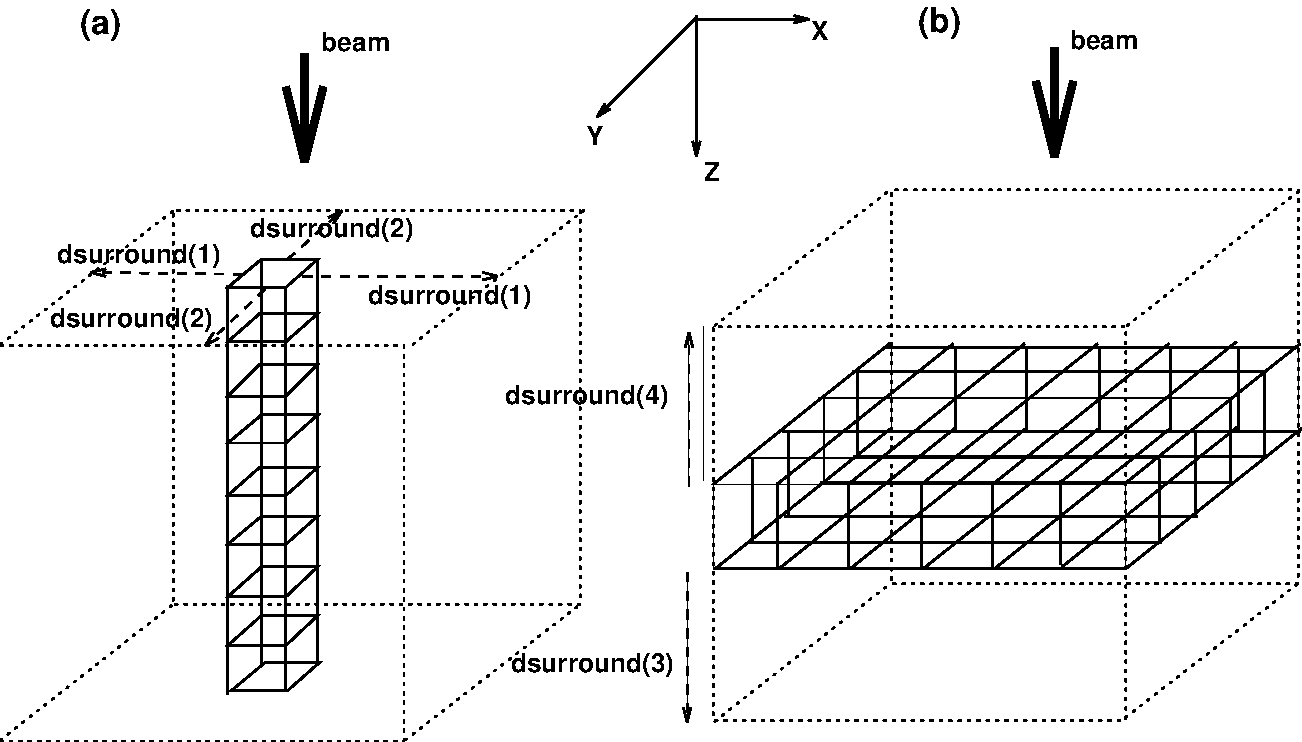
\includegraphics[height=8cm]{figures/dsurround_fig1}
\caption{Two examples of how {\tt dflag} and {\tt dsurround(1...4)} can be used
to
specify a small group of voxels within a larger phantom of the same medium.
In (a) voxels are only specified in a single column for scoring depth-dose,
while the rest of the phantom is defined using {\tt dsurround(1)} and
{\tt dsurround(2)} ({\tt dsurround(3)} and {\tt dsurround(4)} are 0 in this
particular example).  (b) shows voxels specified in a horizontal slice
for scoring the dose profile at a given z value.
In this latter example, the dimensions of the phantom below and above the
slice are defined by {\tt dsurround(3)} and {\tt dsurround(4)} respectively.
{\tt dsurround(1)} and {\tt dsurround(2)} are set to 0 in (b).}
\label{fig_dsurround}
\end{center}
\end{figure}

\lfoot[{{\sffamily \leftmark}}]{{\small Last edited $Date: 2013/09/24 14:49:18 $ }}

Table~\ref{dsurround_table} below shows the results of timing studies
performed using a beam of 10 MeV electrons and a beam
of 6 MV photons incident on a 59x59x10cm water phantom.  For
each beam, 4 cases were simulated: the entire volume filled with 1cm$^{3}$
voxels; 1cm$^{3}$ voxels specified in a column (1x1x10) down
the central (z) axis of the volume (similar to Figure~\ref{fig_dsurround}(a));
1cm$^{3}$ voxels specified in
a vertical slice (1x59x10) through the phantom in the y direction
at x=0; 1cm$^{3}$ voxels specified in a horizontal slice
(59x59x1) through the
phantom at z=2.5cm ($\sim$d$_{max}$)
(similar to Figure~\ref{fig_dsurround}(b)).  In
all cases, simulations were run with and without range rejection.

\begin{table}[htbp]
\caption{Timing results for circular beams of 10 MeV electrons and 6 MV
photons incident on a water phantom.
In all cases, the phantom size is the same (59x59x10 cm$^3$), but the
1x1x1cm$^3$ voxels take up differing parts of the volume (see text).}
\label{dsurround_table}
\begin{tabular}{|p{3cm}|p{3cm}|p{4cm}|p{4cm}|}
\hline
source & number of voxel regions (all 1 cm$^3$) & \multicolumn{2}{|c|}{CPU time (hrs)}\\
\cline{3-4}
       &             & range rejection off & range rejection on \\
\hline
\hline
10 MeV electrons & 59x59x10~~~~~~~ uniform & 0.576 & 0.559 ({\tt ESAVE}=5MeV)\\
\cline{2-4}
(r=10 cm, & 1x1x10 central axis & 0.181 & 0.100 \\
\cline{2-4}
1x10$^{6}$ histories) & 1x59x10 vertical plane & 0.208 & 0.141\\
\cline{2-4}
 & 59x59x1 horizontal plane & 0.345 & 0.300\\
\hline
\hline
6 MV photons & 59x59x10 & 1.623 & 1.525 ({\tt ESAVE}=3MeV)\\
\cline{2-4}
(r=10 cm, & 1x1x10 & 0.785 & 0.479\\
\cline{2-4}
30x10$^{6}$ histories) & 1x59x10 & 0.824 & 0.551\\
\cline{2-4}
 & 59x59x1 & 0.969 & 0.711\\
\hline
\end{tabular}
\end{table}

The table shows that if a depth-dose curve is all that is required, then
specifying voxels only in a 1x1x10cm column can decrease
simulation time by a factor of 5.5 for the electron beam and
a factor of 3 for the photon beam.
In general, the CPU time increases
as the number of voxels specified increases, but orientation of the volume
in which voxels are specified plays a role as well.
The 59x59x1cm horizontal slice
is, relatively, the least efficient use of {\tt dsurround} (saving a factor of
$\sim$2 in CPU time) due to the fact that it has more voxels than the
central-axis phantom and the vertical slice phantom but also due to the fact
that most of the primary and secondary particles from the beam have to be
transported across the
horizontal voxel boundaries defining the slice.  Finally, note that range
rejection is
more efficient when using {\tt dsurround} with a smaller number of
voxels:
turning range rejection on decreases the
simulation time for the case where voxels are only specified in a 1x1x10cm
column by a factor of almost 2, while
its effect on the simulation time when the entire phantom is divided into
voxels is negligible.

Note that this option allows electrons to take much bigger steps in the
{\tt dsurround} regions and this can cause some small inaccuracies unless
the default EGSnrc transport parameters are used.

\section{Pegsless mode}
\indexm{pegsless mode}

As of 2013, DOSXYZnrc can be run independent of the pegs4 cross section data file.  Photon
cross sections had been calculated on the fly since 2006, so the move towards a completely pegsless
version of EGSnrc-based user codes was a logical one.

When running in pegsless mode, all media used in the simulation must be defined
in the {\tt .egsinp} file, between the delimiters, {\tt :start media definition:} and {\tt :stop media definition:}.
{\tt .egsinp} file.  Here, the user has the option of specifying the name of a material data file, containing
\indexm{pegsless mode!material data file}
the compositions, bulk densities, etc, of the media and/or defining media parameters directly in the {\tt .egsinp} file.  The latter method is useful for defining media not included in the material data file or for overriding parameters
in the material data file.  The user also specifies the particle energy limits for cross section calculation:
\indexm{pegsless mode!AE}\indexm{pegsless mode!UE}\indexm{pegsless mode!AP}\indexm{pegsless mode!UP}
{\tt AE} and
{\tt UE} for electrons, {\tt AP} and {\tt UP} for photons.   For more information about the inputs
between the {\tt :start media definition:} and {\tt :stop media definition:} delimiters, including defaults, you are
urged to refer to the BEAMnrc Users Manual\cite{Ro09}.

Pegsless mode is accessible through the DOSXYZnrc GUI by selecting ``Change PEGS4 file'' from the ``File'' menu and
then opting to ``Go PEGSless'' instead of selecting a PEGS4 file.  Once you have done this, a ``Define Media'' button
at the bottom of the main input window becomes active.  Pushing this button will open up a sub-window through
which you have access to the inputs between {\tt :start media definition:} and {\tt :stop media definition:} in
the {\tt .egsinp} file.

\indexm{pegsless mode!running in}
DOSXYZnrc can be run interactively in pegless mode using the command line input:
\begin{verbatim}
dosxyznrc -i inputfile
\end{verbatim}
where {\tt inputfile} is the name of the input file (with no
{\tt .egsinp} extension).

Pegsless batch runs use the command line syntax:
\begin{verbatim}
exb dosxyznrc inputfile pegsless [short|medium|long] [batch=batch_system] [p=N]
\end{verbatim}
This is identical to the syntax of a run with pegs data (see Section~\ref{candrsect} above) but
with the word {\tt pegsless} in place of the name of the pegs data file.

\indexm{pegsless mode!.mederr file}
On termination, pegsless runs output a file, {\tt inputfile.mederr}, containing information about where
the specifications for each medium in the simulation have been read ({\it i.e.} from the material data
file or directly from {\tt inputfile.egsinp}) and various warning messages related to inputs that have
been left blank and have been set to their default values.  The media compositions and settings for other
parameters necessary for calculating cross sections are output to {\tt inputfile.egslst} and
{\tt inputfile.egslog} (for batch runs).

\section{CT Based Phantoms/{\tt ctcreate}}
\indexm{ctcreate}
\indexm{CT!phantoms}

The CT phantom option of DOSXYZnrc allows calculation of dose distributions in
phantoms that are derived from CT data sets. This
allows simulations in realistic anthropomorphic
phantoms. (Please note that the previous sentence does not use the
word patient.)  The creation of CT phantoms from CT data is performed
using the stand-alone code, {\tt ctcreate}.

\indexm{Pinnacle CT}
\indexm{AAPM CT}
\indexm{CT!format!AAPM}
\indexm{CT!format!CADPLAN}
\indexm{CT!format!Pinnacle}
\indexm{CT!format!DICOM}
\indexm{CADPLAN CT}
At this point in time, {\tt ctcreate} supports CT data in DICOM
format (with some restrictions, see below), ADAC
Pinnacle format, and CADPLAN format.
A tool for converting the AAPM CT format into
Pinnacle format is also available.

The process by which CT phantoms are created by {\tt ctcreate}
\indexm{ctcreate}
are outlined here and described in detail in the following sections.

\begin{enumerate}
\item Read in the format of the CT data
\item Read in the CT header parameters (binary or ASCII).
\item Read in the binary CT data.
\item Choose a subset of the CT data set (if desired).
\item Resample the CT data to correspond to volume elements that dose
will be scored in.
\item Convert the CT data to materials and densities for each voxel.
\item Transfer the data via a file to be input to DOSXYZnrc.
\end{enumerate}

\indexm{.egsphant}
\indexm{files!.egsphant}
The relevant CT phantom information
is written into the file, {\tt *.egsphant} (prefix is the same as the
original CT data set name).  A flowchart for the CT phantom code, showing
how it relates to DOSXYZnrc is shown in figure~\ref{fig_ct01}.

Nearly all of the CT phantom functionality takes place outside of
{\tt ctcreate} proper in subroutines.  This
\indexm{ctcreate}
modularity allows for easy changes in the code by ambitious users (for example subroutines for
other CT file formats).  Specifically, this is to provide the user with the
means of reading
their own CT file formats and writing their own dose distribution files
 without rewriting large chunks of
{\tt ctcreate.mortran} and {\tt dosxyznrc.mortran}. This can be accomplished
by creating their
own versions of the subroutines {\tt ReadCT} in {\tt ctcreate.mortran} and
{\tt write\_dose} in {\tt dosxyznrc.mortran}. The
specifications as to what
is required of these subroutines can be found in the codes themselves and
in section~\ref{spec_ReadCT} of this document.

\indexm{CT!coordinate system}
Note that the input CT data set defines the coordinate system for the
calculation, which may be different from the coordinate system of the
accelerator simulation (using BEAM).  For example, for Pinnacle CT
\indexm{Pinnacle CT}
data sets, the Z-axis is typically down the centre of the patient whereas in
the accelerator simulation the Z-axis is the beam's central axis.  This
causes no problems, but must be kept in mind.

\begin{figure}[htbp]
\begin{center}
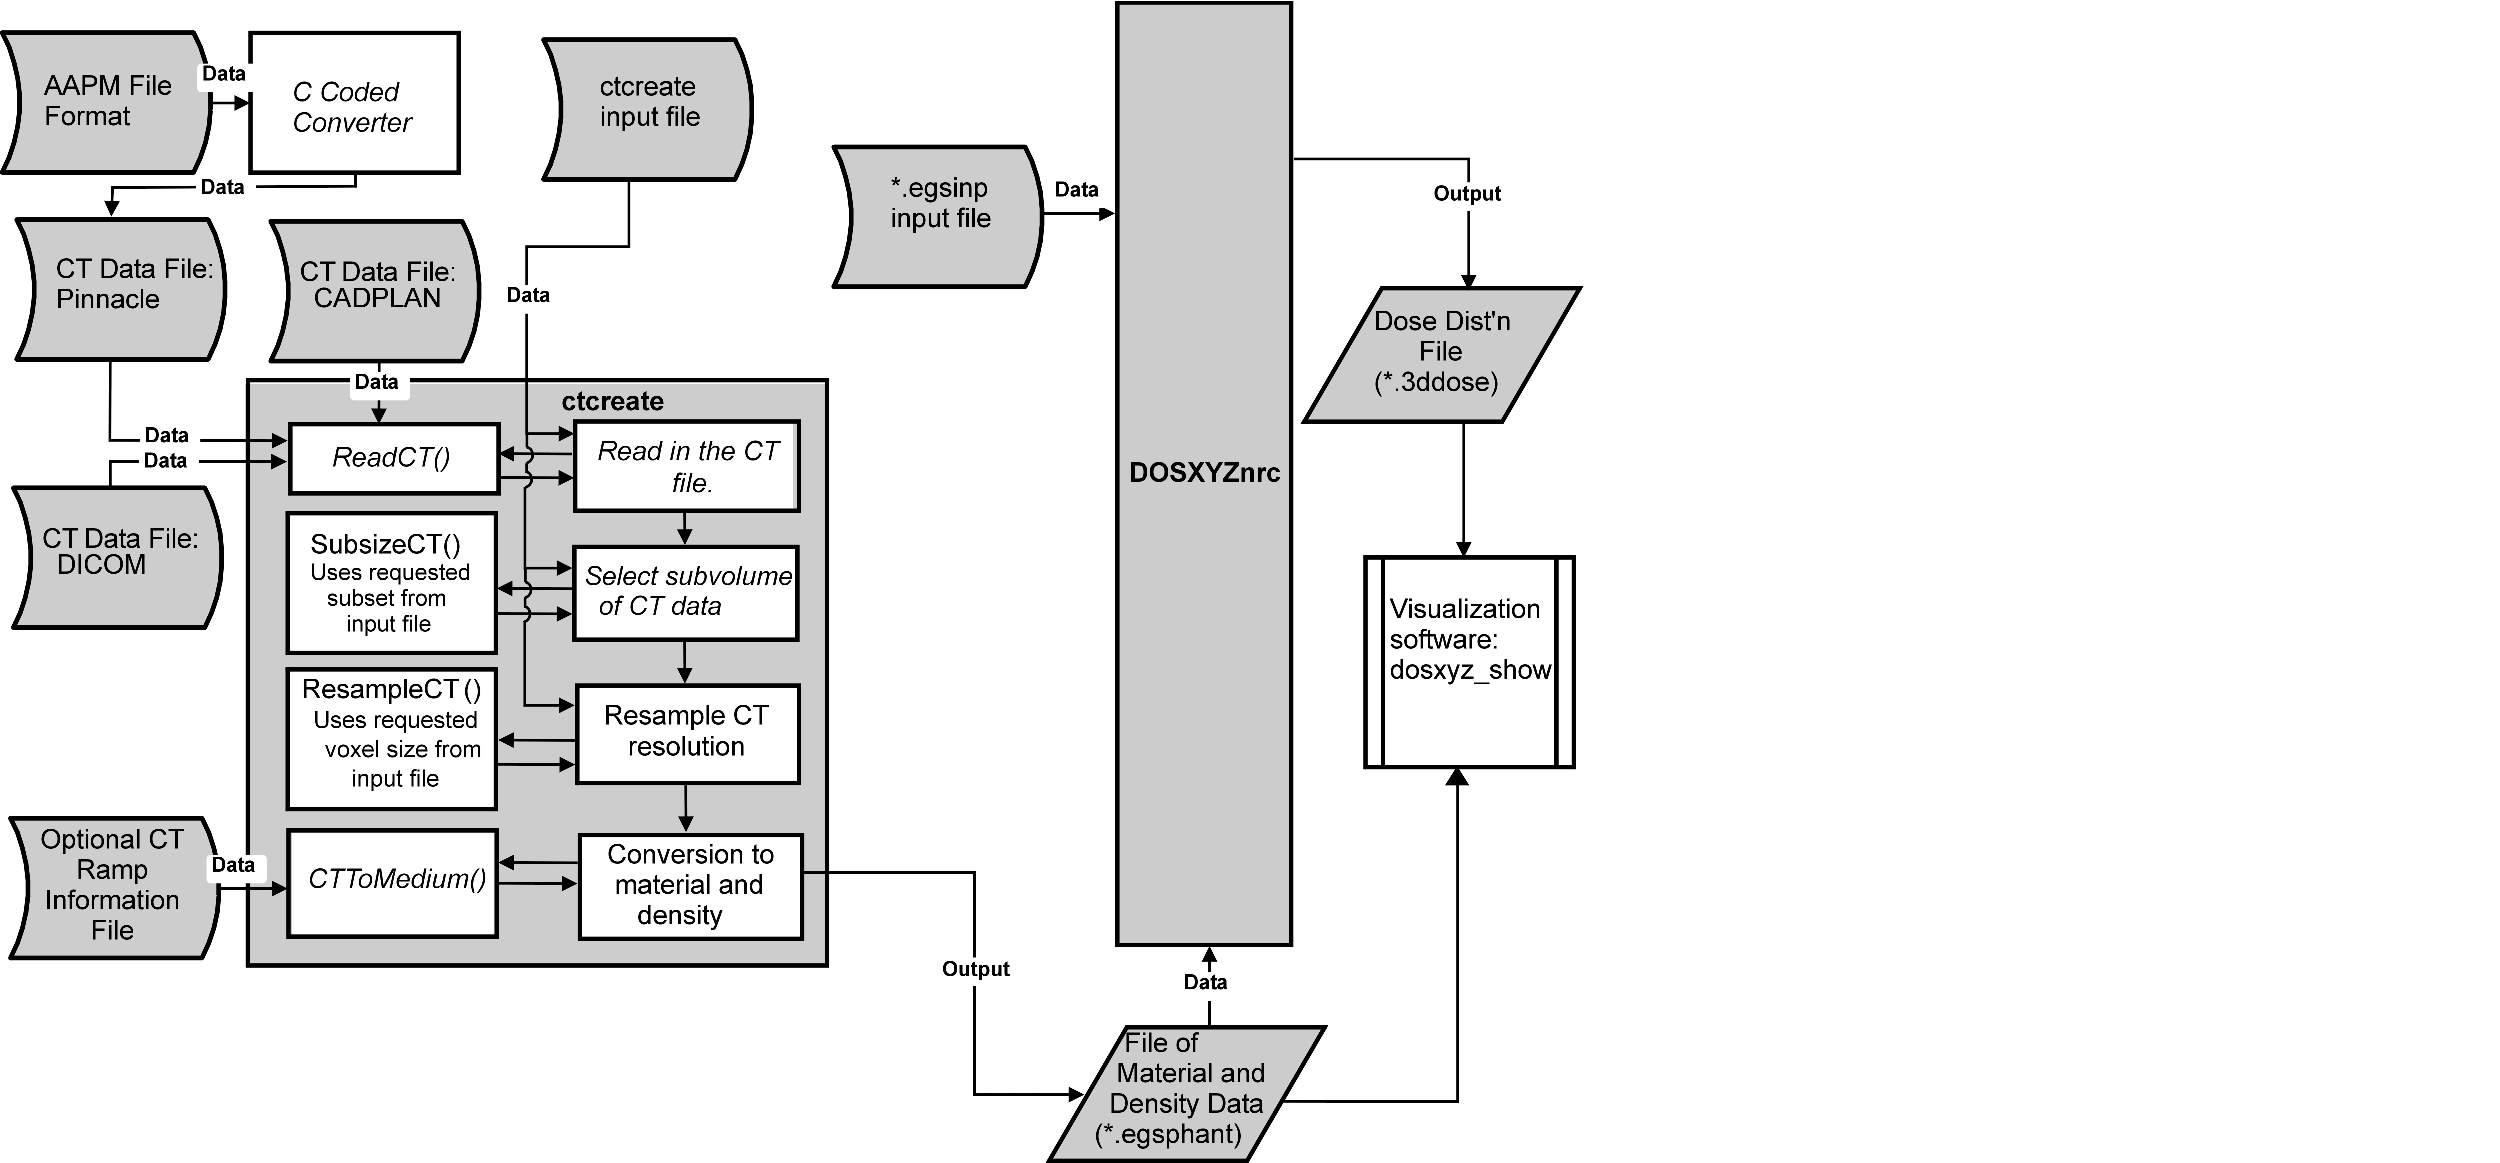
\includegraphics[height=12cm]{figures/ct_fig1}
\caption{A flowchart for use of CT data with  {\tt ctcreate} and DOSXYZnrc. }
\label{fig_ct01}
\end{center}
\end{figure}

\subsection{Using the CT Phantom Option in DOSXYZnrc}

\indexm{CT!option}
\indexm{nmed}
The CT phantom option is used by setting the number of materials,
{\tt nmed} in record 2 of the DOSXYZnrc input file, to zero. This will cause the
program to execute differently than when {\tt nmed} is $>$ 0, and, instead
of geometry, material and density data for the phantom being input explicitly
in the DOSXYZnrc input file,
DOSXYZnrc reads these data from a CT phantom file which has
been created using {\tt ctcreate}.  The input for the
CT and non-CT modes of DOSXYZnrc
are common again after this input (see section~\ref{DOSXYZ_input},
page~\pageref{DOSXYZ_input}).

In short, the input file for DOSXYZnrc is very different if the CT
option is being used.  From section~\ref{DOSXYZ_input} it can be seen
that in CT mode, input records 3-9 in non-CT mode are replaced by
records 3-5, which specify the name of the file containing the CT phantom
data, the transport parameters, and some output parameters.

\subsection{Using {\tt ctcreate}}

\indexm{ctcreate}
\indexm{.egsphant}
\indexm{files!.egsphant}
This section covers the input parameters that {\tt ctcreate} requires
to create a {\tt *.egsphant} CT phantom file that can then be read in and
used by DOSXYZnrc.

It is fairly simple to obtain a
CT phantom from the CT data set since all the required material and geometry
information is contained in the data set.
The additional information that the user is required to provide
are the CT data format, the name of the file containing either the header
info (Pinnacle) or containing the names of the actual CT data files (CADPLAN
and DICOM),
voxel dimensions for the phantom. The user can also select a subset of the full
CT data and specify their own CT ramp (ie function for converting
\indexm{CT!ramp}
CT data to the densities and materials required for the DOSXYZnrc phantom).  Input
of a custom CT ramp is highly recommended.

The following are the input parameters for {\tt ctcreate}.  This description
is found at the beginning of the {\tt ctcreate.mortran} code.
\indexm{ctcreate!input parameters}
\begin{small}
\input{inputs/ctcreate.inp}
\end{small}
\indexm{running ctcreate}

Parameters may be input interactively, by typing:

{\tt ctcreate}

and responding to the prompts;  or stored in an input file
and {\tt ctcreate} run with the input file by typing:

{\tt ctcreate inputfilename}

{\tt ctcreate} input parameters are described in more detail in the subsections below.

\subsubsection{{\tt ctformat}}
\indexm{CT!format}
The first input required by {\tt ctcreate} is the format of the
CT data.  Currently, {\tt ctcreate} supports {\tt Pinnacle}, {\tt
CADPLAN} and {\tt DICOM} formats.
If the data is in AAPM format, then it can be converted to Pinnacle format
using the code
{\tt \$OMEGA\_HOME/progs/ctcreate/CT/AAPM/aapm2pinnacle}
\indexm{aapm2pinnacle}
\indexm{AAPM format}
\indexm{Pinnacle format}
\indexm{CADPLAN format}

\subsubsection{{\tt CTFilename}}
\indexm{CT!data file}
\indexm{CTFilename}
{\tt CTFilename} is the full name of a file, the contents of which depend
on the CT data format:
\begin {description}
\item [Pinnacle format]
\indexm{Pinnacle CT}
{\tt CTFilename} is the full name of the header file of the CT data set
(including the {\tt .header} extension).
The code
will read in all the information that it requires from this file before
moving on to read in the entire binary data file (which has an assumed
extension {\tt .img} and the same prefix as the header file).
  %A sample Pinnacle header file is shown in the next section of this document.
\item [CADPLAN and DICOM formats]
\indexm{CADPLAN CT}
\indexm{DICOM CT}
{\tt CTFilename} is the full name ({\it i.e.} including directory path)
of a file containing the full names of the
individual CT data files (1 file/image slice).  The file names MUST appear
in order of increasing Z position of the slice.
\end{description}

\indexm{.egsphant}
\indexm{files!.egsphant}
On output, the CT phantom will be named:\\
{\tt CTFilename(minus .header extension if using Pinnacle format).egsphant}\\

\subsubsection{{\tt xctsubmin,xctsubmax,yctsubmin,yctsubmax,zctsubmin,zctsubmax}}
\indexm{CT!sub-volume}
\indexm{xctsubmin}
{\tt xctsubmin},{\tt xctsubmax}, {\tt yctsubmin}, {\tt yctsubmax},
{\tt zctsubmin},
and {\tt zctsubmax} are used to create six planes which describe a cube.
The subsection of the original CT data contained in this cube will
be used to create the CT phantom. In this
manner only the portion of interest in the original CT data is used in
the simulation.  This allows the particle simulation
to be performed at a higher resolution than if the calculation used the
entire CT volume, and allows the user to trim some of the air that surrounds
a typical CT image from consideration in the phantom.  Note that if the
sub-volume selected by the user does not fit on an integer number of voxels
from the original CT data, then the sub-volume will automatically be expanded
until it does so.

\subsubsection{{\tt xyz\_xthickness,xyz\_ythickness,xyz\_zthickness}}
\indexm{CT!phantom voxels}
\indexm{voxel size}
\indexm{xyz\_xthickness}
The third line of the input to {\tt ctcreate} is the
spatial resolution that the user requires for the simulation.
{\tt xyz\_xthickness}, {\tt xyz\_ythickness}, {\tt xyz\_zthickness}
are the 3 dimensions of the voxels to be used in the CT phantom.
The maximum voxel dimension in a given direction is
the distance between the planes delimiting the subset of the CT data
to be used in that direction (see previous section).
The minimum voxel dimension in a direction is the distance between
the planes delimiting the subset of CT data in that direction divided
by the maximum number of voxels allowed in that direction (set at
compilation).
{\tt ctcreate} will alert the user when dimensions less than the minimum
or greater than the maximum are input.  Note that, if necessary, the voxel
dimensions will always be increased to fit an integer number of DOSXYZnrc
voxels on the CT sub-volume selected by the user.

\subsubsection{{\tt num\_material}, {\tt material\_ct\_lower\_bound}, and other CT ramp inputs}
\indexm{CT!ramp}

{\tt num\_material} is the
number of materials in the ramp function used
to convert CT number in each voxel to material and density.
If this is set to zero then a
default CT ramp is used in the conversion. The default ramp
is shown in Figure~\ref{fig_ct02} and in the sample input file given in the next section.
{\tt material\_ct\_lower\_bound} defines the lowest CT number of the first ramp
({\it i.e.} the lowest CT number for material  1).  If the default ramp is used, then {\tt material\_ct\_lower\_bound} defaults
to -1024, which is typically the minimum CT number for air in DICOM format data.

If {\tt num\_material} $>$0 then
the CT ramp is read from
the input file.  For each medium in the ramp, there are
two lines of input. \indexm{CT!ramp}
The first of these lines is the name of the material
({\tt material\_name}) which must be identical to a material in the
{\tt PEGS4} material data file being used in the DOSXYZnrc simulation.
The second line specifies the maximum CT number for the medium, {\tt material\_ct\_upper\_bound},
the minimum density of the medium, {\tt material\_density\_lower\_bound}, and the maximum
density of the medium,
{\tt material\_density\_upper\_bound}. Note that the ramp is assumed to be continuous
in CT number.  Thus, for material {\tt n}, {\tt material\_density\_lower\_bound(n)} corresponds
to a CT number of {\tt material\_ct\_upper\_bound(n-1)} (or the overall
minimum CT no. of the ramp, {\tt material\_ct\_lower\_bound}, if
{\tt n}=1), and {\tt material\_density\_upper\_bound(n)} corresponds to
{\tt material\_ct\_upper\_bound(n)}.
Also note that the ramp must be input in order of
increasing {\tt material\_ct\_upper\_bound}.

The CT ramp is then used to determine the medium and density in each voxel of the CT data.
\indexm{CT!ramp}
If a voxel's CT number is $\leq$ {\tt material\_ct\_upper\_bound(n)} and
$>$ \\
{\tt material\_ct\_upper\_bound(n-1)} (or {\tt material\_ct\_lower\_bound} if
{\tt n}=1)
then it is assigned medium {\tt n}. The density is then calculated using a linear
interpolation between the medium's density limits:
\begin{align}
{\tt r}&{\tt hor}_{i,j,k} = {\tt material\_density\_lower\_bound(n)} \nonumber \\
             &+\left(\frac{{\tt material\_density\_upper\_bound(n)}-
 {\tt material\_density\_lower\_bound(n)}}
{{\tt material\_ct\_upper\_bound(n)}-
 {\tt material\_ct\_upper\_bound(n-1)}}\right)        \\
        &*({\tt CT}_{i,j,k}-{\tt material\_ct\_upper\_bound(n-1)}) \nonumber
\end{align}

The default ramp is shown in Figure~\ref{fig_ct02}. This is a modified version of
\indexm{CT!ramp}
a CT ramp given in Kawrakow et al\cite{Ka96a}.  Note that this ramp has been
optimized for typical DICOM format data, where the lowest CT number for air
{\tt material\_ct\_lower\_bound} is -1024.

If the CT number in a voxel is less than {\tt material\_ct\_lower\_bound} then
the medium in that voxel is set to vacuum with density zero.
Those voxels with CT numbers above the
last material's upper CT number ({\tt material\_ct\_upper\_bound(num\_material)})
will have the density set to the maximum
density for the last material.

\begin{figure}[H]
\begin{center}
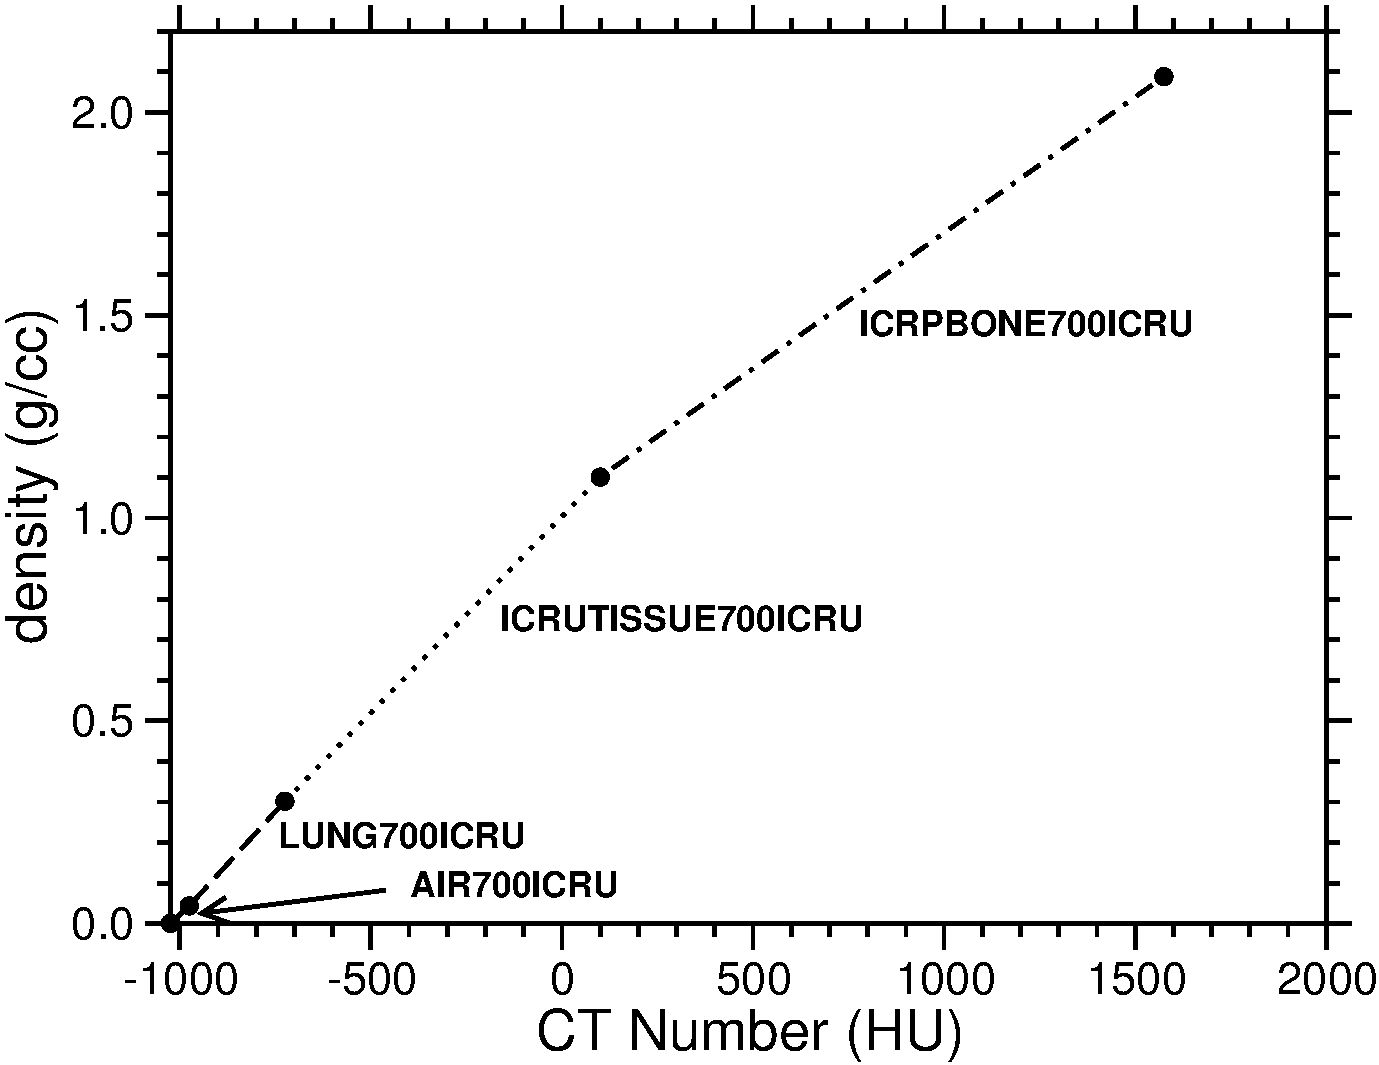
\includegraphics[width=10.5cm]{figures/CTramp}
\caption{The default ramp for converting CT values to material and
density in {\tt ctcreate} modified from Kawrakow et al\cite{Ka96a}.}
\label{fig_ct02}
\end{center}
\end{figure}
\indexm{CT!ramp}

The default CT ramp may be suitable for displaying a {\tt .egsphant} file
using {\tt dosxyz\_show}\cite{Ka98} and for example calculations.  However,
we strongly recommend that you explicitly enter your own CT ramp function
for more detailed simulations, since the CT ramp is
dependent upon the imager and the data acquisition method.

\subsection{Sample {\tt ctcreate} CT Phantom Input File}
\indexm{ctcreate!sample input}
Table~\ref{ctinpex} shows an example {\tt ctcreate} input file, and
a sample DOSXYZnrc input file (excluding EGSnrc inputs)
which uses the CT phantom data from {\tt ctcreate}.

\vspace*{-0.5cm}
\begin{table}[htbp]
%\begin{tabular}{|p{8cm}p{7.7cm}|}
\caption{Sample input files for {\tt ctcreate} and DOSXYZnrc}
\begin{tabular}{|p{7cm}p{8.7cm}|}
\hline
\bf{Input Parameter} & \bf{Description of input fields.} \\
\multicolumn{2}{|c|}{\bf for {\tt ctcreate}      } \\
{\tt DICOM} & CT data is in DICOM format \\
{\tt CTfname} & in DICOM format, this is the name of a file containing the names of the individual image slices (in order
of increasing Z).
\\
%\hline
{\tt -17.64,17.64,-17.64,17.64,-0.7,4.3}
&
The subvolume of the CT data set
that is to be used for the phantom.
\\
%\hline
{\tt 1.0, 1.0, 1.0 }
&
The phantom voxel size.
\\
%\hline
{\tt 4, -1024}
&
{\tt num\_material}, {\tt material\_ct\_lower\_bound}.
If {\tt num\_material}=0
the default ramp will be used.
The default values are
listed explicitly in this example.
\\
%\hline
{\tt AIR700ICRU }
&
The material\_name for the first material.
\\
%\hline
{\tt -974,0.001,0.044}
&
CT ramp parameters for the first material:\\
&{\tt  material\_ct\_upper\_bound}, \\
&{\tt material\_density\_lower\_bound},\\
&{\tt material\_density\_upper\_bound}
\\
%\hline
{\tt LUNG700ICRU }
&
The material name for the second material.
\\
%\hline
{\tt -724,0.044,0.302}
&
The ramp parameters for the second material. \\
%\hline
{\tt ICRUTISSUE700ICRU} & The material name for the third material.
\\
%\hline
{\tt 101,0.302,1.101} & The ramp parameters for the third material.
\\
%\hline
{\tt ICRPBONE700ICRU} & The material name for the fourth material.
\\
%\hline
{\tt 1976,1.101,2.088} & The ramp parameters for the fourth material.
\\
\hline
\multicolumn{2}{|c|}{\bf for DOSXYZnrc} \\
%\hline
{\tt Sample CT Input File } & Title of the simulation and phantom. \\
%\hline
0 & {\tt NMED } - If this is zero the code switches to CT\_Phantom mode. \\
%\hline
{\tt CTfname.egsphant} & The name of the CT phantom file.\\
{\tt 0.7,0.01,5.0} & {\tt ECUTIN}, {\tt PCUTIN}, {\tt SMAX} (dummy inputs)\\
{\tt 1,0,1} & {\tt zeroairdose}, {\tt doseprint} and {\tt MAX20} \\
%\hline
{\tt -1,0,-1.25,1.25,-2.25,2.25,90.0,} & The source description record.
At this point the \\
{\tt 90.0,0.0} &CT phantom input meets up with the manual\\
& phantom inputs.
\\
%\hline
{\tt 0}
&
monoenergetic particle spectrum.
\\
%\hline
{\tt 20.0 }
&
particle energy.
\\
%\hline
{\tt 100,0,500.,7,3,100.,0,0,0,1,5.0,} & Monte Carlo information (note range rejection \\
\hspace*{1cm}{\tt 0,0,0,0}&below 5MeV).  \\
%\hline
\hline
\end{tabular}
\label{ctinpex}
\end{table}

\subsection{Location of {\tt ctcreate} and How to Compile It}
\label{comp_ctcreate}
{\tt ctcreate.mortran} and related files
(see section~\ref{filesect} for a complete list)
\indexm{ctcreate!installation}
reside in the subdirectory {\tt \$OMEGA\_HOME/progs/ctcreate}.
Normally, it is compiled as part of the OMEGA/BEAM installation
(see the BEAMnrc Manual\cite{Ro04a} for installation instructions), however
it can be compiled separately by going into this directory and
typing {\tt make}.

\subsection{{\tt ReadCT()} Subroutines}
\label{spec_ReadCT}
\indexm{ReadCT}
\indexm{CT!format!AAPM}
\indexm{CT!format!CADPLAN}
\indexm{CT!format!DICOM}
\indexm{CT!format!Pinnacle}
{\tt ReadCT} is the most important subroutine in {\tt ctcreate}.  It handles
the reading in of header information and binary CT data.  Currently, there
are three {\tt ReadCT} subroutines within {\tt ctcreate}, one for each of the CT formats
supported: {\tt ReadCT\_Pinnacle} for Pinnacle, {\tt ReadCT\_CADPLAN}
for CADPLAN data and {\tt ReadCT\_DICOM} for DICOM data.

\subsubsection{{\tt ReadCT\_Pinnacle}}
\indexm{ReadCT\_Pinnacle}
\indexm{CT!format!Pinnacle}

{\tt ReadCT\_Pinnacle} is contained
within the {\tt ctcreate.mortran} file and calls
other subroutines and functions in this file:
\begin{description}
\indexm{ReadReal}
\indexm{ReadInt}
\indexm{read\_ct\_data}
\indexm{swap\_bytes}
\item[{\tt ReadReal}] Reads real values from the image header ({\tt .header}) file.
\item[{\tt ReadInt}] Reads integer values from the header file.
\item[{\tt read\_ct\_data}] Reads binary CT data from the image ({\tt .img})
file.
\indexm{swapping bytes}
\item[{\tt swap\_bytes}] Swaps bytes of CT data if there is a
byte order mismatch between the data and the machine you are using.
\end{description}

Note that in Pinnacle format CT numbers are $>$ 0.  Thus, the default CT ramp
in {\tt ctcreate} cannot be used to convert CT numbers to media and densities.
The example {\tt ctcreate} inputfile, {\tt \$OMEGA\_HOME/progs/ctcreate/ctcreate\_examples/CT\_create.inp}
(used in Lab VI in the BEAMnrc Workshop), is used to convert Pinnacle format data and
contains a custom CT ramp which is just the default ramp shifted up by 1025 HU.

\subsubsection{{\tt ReadCT\_CADPLAN}}
\indexm{ReadCT\_CADPLAN}
\indexm{CT!format!CADPLAN}
{\tt ReadCT\_CADPLAN} is also contained
within the {\tt ctcreate.mortran} file.
Unlike {\tt ReadCT\_Pinnacle}, {\tt ReadCT\_CADPLAN} is a self-contained subroutine.
Byte swapping is not required since single bytes are read at a time.


\subsubsection{{\tt ReadCT\_DICOM.c}}
\indexm{CT!format!DICOM}
\indexm{ReadCT\_DICOM}
{\tt ReadCT\_DICOM.c} is a separate C routine whose object file is linked
to {\tt ctcreate} at compile time.  {\tt ReadCT\_DICOM.c} is automatically
compiled when you {\tt make} ctcreate.
{\tt ReadCT\_DICOM.c} requires the C header file {\tt tags\_ct.h}, which
defines hexadecimal tags, or labels, for the DICOM data.  These tags
are defined in the DICOM standard, and if the user modifies
{\tt ReadCT\_DICOM.c} to deal with additional tags, then these can
be added to the {\tt tags\_ct.h} file.
Currently,
{\tt ReadCT\_DICOM} assumes
\indexm{little endian byte order}
\indexm{big endian byte order}
the DICOM data has been collected on a machine with little endian byte order
(ie compatible with Linux), however, if the data was collected on a machine
with big endian byte order, you must go into {\tt ReadCT\_DICOM.c} and
change the line:
\indexm{DICOM\_ENDIAN}
\begin{verbatim}
#define DICOM_ENDIAN 1
\end{verbatim}
to:
\begin{verbatim}
#define DICOM_ENDIAN 0
\end{verbatim}
and recompile {\tt ctcreate}.  The endianness of the machine you
are running {\tt ctcreate} on is automatically detected by
{\tt ReadCT\_DICOM} and then bytes are swapped if necessary.

The DICOM format is known to vary from imager to imager and institute
to institute.  Thus, we cannot guarantee that {\tt ReadCT\_DICOM} will
work with your images without modification.  As a minimum,
the current version of {\tt ReadCT\_DICOM} requires the following
information in the image (slice) header(s):
\begin{enumerate}
\item Number of rows (data tag {\tt 0x00280010}).  This defines the number of voxels in the X-direction.
\item Number of columns (data tag {\tt 0x00280011}). This defines the number of voxels in the Y-direction.
\item Pixel spacing (data tag {\tt 0x00280030}).  Defines the X- and Y-dimensions of the voxels.
\item Image position (data tag {\tt 0x00200032}). Defines the (X,Y,Z) of the centre of the first voxel.  The position
of the first slice (slice with lowest Z) is used to determine the X-, Y- and
Z-offset (starting position) of the CT data, and the Z-positions of the first two slices are used
to established voxel Z-dimension ({\it i.e.} slice thickness).
The Z-positions of slices as read from the header are also used to
sort slices in order of increasing Z, in case the user has not already done so
in the file containing the slice names.
\item A pixel data tag ({\tt 0x7fe00010}) indicating the size of the data array in bytes.  This tag must appear last in the
header, immediately preceding the CT data itself.
\end{enumerate}

{\tt ReadCT\_DICOM} assumes slices are contiguous in Z.  Thus, once the Z-position of the first slice and slice thickness (Z-dimension of voxels) are
established, {\tt ReadCT\_DICOM} positions subsequent slices so that there are no gaps
or overlaps between them.  A warning message is output if the Z-position of
a slice determined by {\tt ReadCT\_DICOM} does not equal the Z-position
of the slice as read from the image position in its header.

We note that {\tt ReadCT\_DICOM.c} has limited flexibility in terms of slice
layout, and it has not been
tested on all possible variations of the DICOM format.  Therefore, if you
require more flexibility or are having trouble converting your DICOM files, you
are strongly urged to either modify {\tt ReadCT\_DICOM} or use your own
stand-alone routine for converting DICOM images to {\tt .egsphant} files.

\indexm{Nick Reynaert}
The initial version of {\tt ReadCT\_DICOM.c} was provided by Nick Reynaert at the University of Ghent.

\subsubsection{Generic {\tt ReadCT}}
\indexm{ReadCT!Generic}

Essentially, {\tt ReadCT} is the subroutine or stand-alone
code which the user will have to
\indexm{ReadCT specs}
customize or program from scratch to deal with any CT format not currently
handled.  The structure and number of subroutines within {\tt ReadCT} is
largely a matter of the programmer's taste.  However, if {\tt ReadCT} is
to be included in {\tt ctcreate} (or linked as an object file when compiling
{\tt ctcreate}), it must
pass certain essential data back to {\tt ctcreate}.   An example call to
a generic {\tt ReadCT} routine is:

\noindent {\tt Subroutine ReadCT(fname,asize,ctdata,offset,vsize,error)}

\noindent where {\tt fname} is a character string containing the name of the
particular CT data set.  The essential CT data returned to {\tt
ctcreate} are:
\begin {description}
\item [{\tt asize(3)}]  An array returning the number of CT voxels in the
                     x,y,z directions.
\item [{\tt vsize(3)}]  An array returning the dimensions of the CT voxels

\item [{\tt offset(3)}] An array returning the lower bounds of the CT data
                      in the x,y,z directions in cm.
\item [{\tt ctdata(\$CTIMAX,\$CTJMAX,\$CTKMAX)}] A 3-D integer array
           returning the CT data (Hounsfield numbers).  In {\tt ctdata},
    {\tt x}$\rightarrow${\tt i},
    {\tt y}$\rightarrow${\tt j},
    {\tt z}$\rightarrow$ {\tt k}, so that {\tt ctdata(i,j,k)} is
    equal to the Hounsfield number in the voxel with lower bounds
    {\tt x=offset(1)+(i-1)*vsize(1)}, {\tt y=offset(2) +} {\tt (j-1)*vsize(2)},
    {\tt z=offset(3)+} {\tt (k-1)*vsize(3)} and
    upper bounds {\tt x=offset(1)+} {\tt i*vsize(1)},
    {\tt y=offset(2)+} {\tt j*vsize(2)}, {\tt z=offset(3)+} {\tt k*vsize(3)}
\item [{\tt error}] Returns the error status of the CT read operation.
                    Currently not used.
\end {description}

\subsection{Description of the {\tt *.egsphant} File}
\label{egsphantsect}
\indexm{.egsphant}
\indexm{files!*.egsphant}
The {\tt *.egsphant} file output by {\tt ctcreate} or by DOSXYZnrc itself
is an ASCII file
containing the following information necessary for DOSXYZnrc to simulate
the CT phantom and for the display program, {\tt dosxyz\_show}\cite{Ka98},
to display the density information:
\begin{enumerate}
\item The number of media in the phantom
\item The names of the media
\item The {\tt ESTEPE} value for each medium (now a dummy input)
\item The number of voxels in the X, Y and Z directions
\item A list of the voxel boundaries in the X direction
\item A list of the voxel boundaries in the Y direction
\item A list of the voxel boundaries in the Z direction
\item For each Z slice, an X-Y array containing the medium
      number in each voxel
\item For each slice in the Z direction, an X-Y array containing the densities
      in each voxel
\end{enumerate}
\vspace*{-0.3cm}
In addition to passing the necessary medium information to DOSXYZnrc, the X-Y
arrays of medium numbers (item 8 above) provide a rough slice-by-slice
view of the CT phantom.  A sample X-Y array of medium numbers from one slice of a CT phantom derived
from a lung image is shown below (hold at a distance, and raw data on
screen is easier to see):

\input{inputs/mednoarray.inp}

The user can use these slice-by-slice views to
determine whether the CT data is being read in correctly by {\tt ReadCT}
or to verify that the sub-volume of the original CT data selected
includes the physiology of interest.

\subsection{Files and Macros for implementation.}
Below is a short description of the files and macros required to compile
and run {\tt ctcreate} and DOSXYZnrc with CT phantoms.
\indexm{ctcreate!files and macros}

\begin{description}
\item[{\tt dosxyznrc\_user\_macros.mortran}]
{\tt ctcreate} uses the version stored in\\
{\tt \$HEN\_HOUSE/user\_codes/dosxyznrc}
to obtain {\$IMAX}, {\$JMAX} and {\$KMAX},
the maximum X, Y and Z dimensions of the CT phantom allowed in DOSXYZnrc.

\item[{\tt \$CTIMAX, \$CTJMAX, \$CTKMAX }]
Macros defining the maximum X, Y and Z dimensions of the CT data to be read in.
These macros are in {\tt ctcreate.mortran}

\item[{\tt lnblnk1.mortran}] {\tt MORTRAN} macro to provide the
FORTRAN {\tt lnblnk} function for Linux, rs6000 and HP9000 machines.
{\tt ctcreate} makes extensive use of this function and DOSXYZnrc uses it
in CT phantom mode.  It
is read from the {\tt \$HEN\_HOUSE/src} directory
\end{description}

\section{Known Bugs/Restrictions}

A resumed run that uses a phase space source with particle recycling will
not produce dose/uncertainty results identical to a single run with
the same total number of histories.  This is because the last particle
used before resuming may not have been recycled the full
{\tt NRCYCL} times, and resuming automatically skips to the next particle.
Results will agree within uncertainty, however.

It is recommended that when using the built-in parallel processing
functionality you do not resume parallel runs that use
a phase space source.  In this case, parallel jobs have lost track
of which chunks of the phase space source they were using in the
original run and the uncertainty analysis after recombining the
resumed runs will not take into account correlations due to reusing
chunks of the phase space source.

\section{Acknowledgments}

Charlie Ma was a major contributor to the DOSXYZ code and was the senior
author of the original DOSXYZ manual. Since he is not directly involved
with DOSXYZnrc, he is no longer an author of the manual, but his
contribution to the original code while he was at NRC still plays a
significant role in the current version.


A variety of people have contributed various pieces of code to the
DOSXYZnrc program.  We wish to thank: Julie Zachman of UW for providing
the aapm2pinnacle tool; Daryoush Sheikh-Bagheri for developing PAW
macros for displaying dose distributions and CT files; Geoff Zhang and
Daryoush again for extensive use of the code and drawing our attention
to bugs; Alex Bielajew for early work on the code; Marc Lauterbach and
Joerg Lehmann for initial coding to read CADPLAN CT data sets.
We also wish to thank Paul Reckwerdt for his work on the original code to
read Pinnacle CT data sets; Mark Holmes for his extensive work on reading
CT data and for coding the correlated sampling routines\cite{Ho99}; Brian
Geiser for the BTREE beam modeling method\cite{Ge95}.  \indexm{CADPLAN CT}

\begin{latexonly}
\section{References}
\end{latexonly}
\renewcommand{\rightmark}{References}
\indexm{references}
\typeout{****references start here}
\setlength{\baselineskip}{0.4cm}
\vspace*{-1cm}
\bibliography{../irs}
\bibliographystyle{unsrt}


\newpage
\setlength{\baselineskip}{0.5cm}

%%%%%%%%%%%%%%%%%%%%%%%%%%%%%%%%%%%%%%%%%%%%%%%%%%%%%%%%%%%%%%%%%%%%%%%%%%%%%%%
%
%  EGSnrc dosxyznrc manual
%  Copyright (C) 2021 National Research Council Canada
%
%  This file is part of EGSnrc.
%
%  EGSnrc is free software: you can redistribute it and/or modify it under
%  the terms of the GNU Affero General Public License as published by the
%  Free Software Foundation, either version 3 of the License, or (at your
%  option) any later version.
%
%  EGSnrc is distributed in the hope that it will be useful, but WITHOUT ANY
%  WARRANTY; without even the implied warranty of MERCHANTABILITY or FITNESS
%  FOR A PARTICULAR PURPOSE.  See the GNU Affero General Public License for
%  more details.
%
%  You should have received a copy of the GNU Affero General Public License
%  along with EGSnrc. If not, see <http://www.gnu.org/licenses/>.
%
%%%%%%%%%%%%%%%%%%%%%%%%%%%%%%%%%%%%%%%%%%%%%%%%%%%%%%%%%%%%%%%%%%%%%%%%%%%%%%%
%
%  Authors:         Blake Walters, 2001
%                   Iwan Kawrakow, 2001
%                   Dave Rogers, 2001
%
%  Contributors:    Frederic Tessier
%                   Marc-Andre Renaud
%
%%%%%%%%%%%%%%%%%%%%%%%%%%%%%%%%%%%%%%%%%%%%%%%%%%%%%%%%%%%%%%%%%%%%%%%%%%%%%%%


%Some conventions:
%	DOSXYZnrc, the code name is in capitals, standard font
%	all file names are in {\tt   }  or \verb+    +
%	the code name ctcreate is also {\tt ctcreate}
%
\documentclass[12pt,twoside]{article}      %twoside messes up indexm and keys
%\usepackage{showkeys}   %this messes up some split commands

%\usepackage[breaklinks]{hyperref}
\usepackage{hyperref}
\hypersetup{colorlinks=true, citecolor=blue, linkcolor=blue, filecolor=blue, urlcolor=blue}
\urlstyle{same}

\usepackage{html}
\usepackage{fancyhdr}
\usepackage{amsmath}  %changed from amstex which is now obsolete
\usepackage{float}
\usepackage{rotating}
\usepackage{enumitem}
\setlength{\textwidth}{16.51cm}
\setlength{\textheight}{23.5cm}
\setlength{\oddsidemargin}{0.0in}
\setlength{\evensidemargin}{0.0in}
\setlength{\topmargin}{-1.5cm}
\setlength{\parindent}{1.5em}
\setlength{\topsep}{0ex}
\setlength{\itemsep}{0ex}

\newcommand{\Co}{$^{60}$Co}
\newcommand{\parsp}{~\hspace*{1.5em}}
\setlength{\parskip}{0.1in}
\setlength{\baselineskip}{0.4in}
\newcommand{\head}[1]{\begin{center}\begin{Large}{\bf #1}
                                              \end{Large}\end{center}}
\newcommand{\cen}[1]{\begin{center} #1 \end{center}                   }
\newcommand{\etal}{{\em et.al.}}
\newcommand{\etc}{{\em etc}}

%*** UW does not have the following files and needs them
%DR  You must have this to use latex2html

\renewcommand{\footrulewidth}{0.4pt}
\renewcommand{\headrulewidth}{0.4pt}

%\rfoot[{\sffamily {\rightmark}}]{{\sffamily {\rightmark}}}

\lhead[{\sffamily \thepage~}]{{\sffamily NRCC Report PIRS-794(revB) }}
\rhead[{\sffamily DOSXYZnrc Users Manual}]{{\sffamily ~\thepage}}
\rfoot[{\sffamily \rightmark}]{{\sffamily \leftmark}}
\lfoot[{{\sffamily \leftmark}}]{{\small Last edited $Date: 2013/09/24 14:49:18 $
}}

\cfoot{}

\makeindex
\newcommand{\indexm}[1]{\index{#1}}
%Use the above for final runs  - following is for drafting
%\newcommand{\indexm}[1]{\marginpar{{\tiny {\sf #1}}}\index{#1}}
%above doesn't work well with twosided

\renewcommand{\refname}{}


\begin{document}

\begin{htmlonly}
For information about the authors and/or institutions involved with this
work, use the links provided in the author list.\\
\begin{rawhtml}
<br><br>
\end{rawhtml}

\begin{rawhtml}
<br><br>
\end{rawhtml}

Postscript versions of the entire paper are available.  You may have to
download the compressed version to disk, uncompress or gunzip them and
then read or print them.
\htmladdnormallink{(pdf version 2.0 Mb)}{pirs794.pdf}
\htmladdnormallink{(uncompressed version 4.5 Mb)}{pirs794.ps}
\htmladdnormallink{(gzip version 2.2 Mb)}{pirs794.ps.gz}
\begin{rawhtml}
<br>
\end{rawhtml}

Use the Up button to get back to this page from within the document.
\begin{rawhtml}
<BR> <HR> <P>
\end{rawhtml}
\copyright
Copyright 1995-2021, National Research Council of Canada
Ottawa
\begin{rawhtml}
<BR> <HR> <P>
\end{rawhtml}
\end{htmlonly}

\pagestyle{empty}

\vspace*{-2cm}

\title{DOSXYZnrc Users Manual}
\begin{center}
{\sffamily \bfseries \Huge DOSXYZnrc Users Manual \vspace{5mm}\\}
\begin{large}
B. Walters, I. Kawrakow and D.W.O. Rogers \\
\end{large}
%\vspace*{0.3cm}
{Ionizing Radiation Standards}\\
{National Research Council of Canada,}
Ottawa K1A 0R6\\

Printed: \today  \vspace{7mm}\\
\hfill NRCC Report {\sf PIRS-794revB       }\\

%\maketitle
\vspace*{-2cm}
\begin{htmlonly}       %%%%%%%%%%%%%%%%%%%%%%%%%%%%%%%%%%%%%%%%%%%%%%
\begin{rawhtml}
<center>
\end{rawhtml}
\end{htmlonly}       %%%%%%%%%%%%%%%%%%%%%%%%%%%%%%%%%%%%%%%%%%%%%%
\begin{figure}[H]
\begin{center}
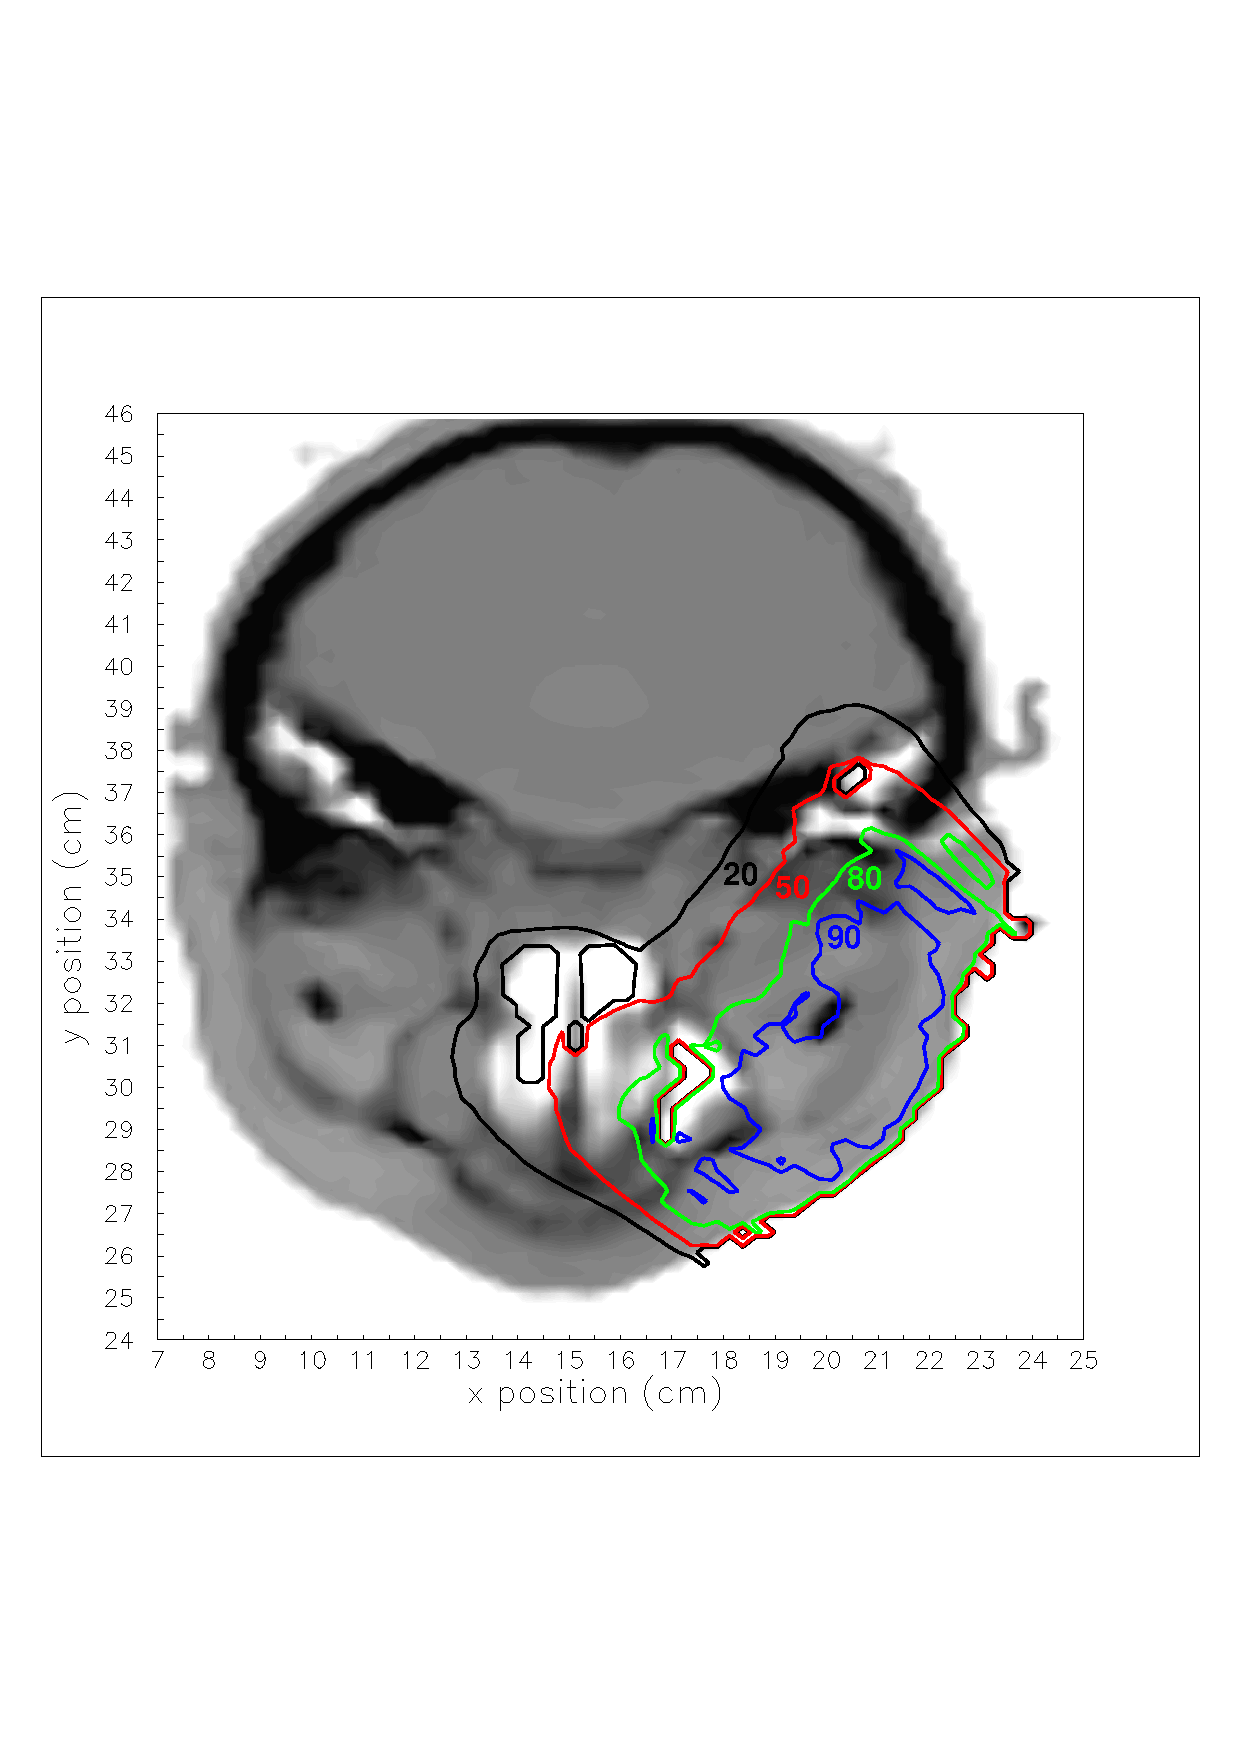
\includegraphics[height=20cm]{figures/CT_example_msmodel}
\end{center}
\end{figure}
\begin{htmlonly}       %%%%%%%%%%%%%%%%%%%%%%%%%%%%%%%%%%%%%%%%%%%%%%
\begin{rawhtml}
</center>
\end{rawhtml}
\end{htmlonly}       %%%%%%%%%%%%%%%%%%%%%%%%%%%%%%%%%%%%%%%%%%%%%%


\vfill
\copyright NRC Canada, 2021
\end{center}

\newpage
\pagestyle{fancy}
\pagenumbering{arabic}
\setcounter{page}{2}

\newpage

\setlength{\parindent}{0em}

\begin{center}
\begin{Large}
{\bf Abstract}
\end{Large}
\end{center}
\indexm{abstract}
DOSXYZnrc is an EGSnrc-based Monte Carlo simulation code for calculating
dose distributions in a rectilinear voxel phantom and is based directly
on the DOSXYZ code developed for the EGS4 code system (see NRC Report
PIRS-509B). DOSXYZnrc is part of the OMEGA-BEAM system of codes developed
at NRC.  Density and material in every voxel may vary.  A variety of beams
may be incident on the phantom, including full phase-space files from
BEAMnrc  and beams characterized using Beam Characterization models. The
companion program {\tt ctcreate} is capable of reading in a CT data set
of Hounsfield numbers and converting it into the information needed by
DOSXYZnrc to simulate transport in a phantom (i.e.  ~the appropriate
material and density are specified in each voxel).  Any of the available
beams can be incident on this CT phantom.  The code includes a resume
option and can be run on parallel computing platforms.  The statistical
analysis is based on a history by history method as opposed to the batch
method used in DOSXYZ.

This user's manual covers general DOSXYZnrc inputs, geometries and outputs.  It
contains information on how to compile and run DOSXYZnrc using the EGSnrcMP
system. It also describes
the use of {\tt ctcreate}.

\begin{latexonly}
\vspace{11.5cm}
\end{latexonly}

\rule{16.3cm}{0.6mm}\\
\begin{small}
The figure on the front page shows a PAW visualisation of the isodose
curves from a DOSXYZ simulation in which a Clinac 2100c 18MeV electron
beam (simulated using a multiple-source model--with 35 million initial
histories) was
incident on the head and neck of a CT phantom.  The visualisation was
implemented by Daryoush Sheikh-Bagheri.

\end{small}

\newpage

\indexm{contents}
\tableofcontents

\newpage

%\pagestyle{myheadings}

\section{Introduction}

\subsection{Overview}
DOSXYZnrc is a general-purpose Monte Carlo EGSnrc\cite{Ka99a,KR00}
\indexm{EGSnrc}
user-code for 3-dimensional absorbed dose calculations. EGSnrc/DOSXYZnrc
simulates the transport of photons and electrons in a Cartesian volume and
scores the energy deposition in the designated voxels. DOSXYZnrc is ``stand
alone'', in the usual EGSnrc sense in that it is controlled by
the {\tt \*.pegs4dat} and {\tt \*.egsinp} files and
is capable of writing out ASCII formatted dose distribution arrays.  The
code uses the EGSnrcMP system which is described in detail in its own
Users Manual\cite{Ka03}.
There is also a graphical user interface (GUI) which allows
input files to be created and executed graphically\cite{TR99}.  Much of the information
in this manual is conveniently accessible via the GUI's help files.


The geometry is a rectilinear volume with
\indexm{geometry coordinate system}
the X-Y plane on the page,  X to the right, Y down the page
and the Z-axis into the page.
Voxel dimensions are completely variable in all three directions. Every
voxel (volume element) can have different materials and/or varying
densities (for use with CT data).  The code allows sources such as a
monoenergetic diverging or parallel beam, phase-space data generated by a
BEAMnrc simulation, or a model-based beam reconstruction produced by BEAMDP.
\indexm{BEAMDP}

DOSXYZnrc has a number of important and unique features such as dose
component calculations, a wide variety of source configurations and beam
reconstruction techniques, CT to phantom conversion
(via {\tt ctcreate}), resume capabilities, phase-space redistribution, \etc.
\indexm{ctcreate}

{\tt ctcreate} is a stand alone program which converts CT data sets into the
data needed for DOSXYZnrc to do a simulation. At present it handles ADAC
Pinnacle, AAPM, CADPLAN and DICOM formats for the CT files.
\indexm{Pinnacle CT}
If you develop extensions, why not
\indexm{CADPLAN CT}
\indexm{DICOM CT}
share them with your colleagues?  Send them to us and we will integrate
them into the standard distribution with full acknowledgement of the
source.

The DOSXYZnrc code, in common with the BEAMnrc system is written for a
preprocessor of Fortran77 called {\tt MORTRAN}. The user does not need
to know {\tt MORTRAN} to use the code, but its elements are needed for
modifications (see refs~\cite{Ne85} or \cite{KR00}).

\subsection{History of DOSXYZnrc}

\indexm{history of DOSXYZnrc}

DOSXYZ started out as a demonstration code that Dave Rogers wrote in March
1986 to show Ralph Nelson that special purpose coding of rectilinear
voxels was faster than using Ralph's more general macros.  At about that time
it was used to estimate the time required to do a full Monte Carlo
treatment planning calculation and the results published 3 years later in
a book chapter\cite{RB90}.  It then became the basis for a Monte Carlo
timing benchmark\cite{BR92} which was regularly updated and available
on the WWW for many years (until 2000).
The OMEGA project took this code over and
added a variety of different source routines with coding contributions
from Charlie Ma, Bruce Faddegon, George Ding, Dave Rogers,  Alex Bielajew,
and Paul Reckwerdt.  More recent modifications have reduced the array
space used by the code, and added beam characterization inputs (Charlie
Ma), btree inputs, (Brian Geiser, but no longer supported), correlated
sampling (Mark Holmes, but no longer supported).
Blake Walters and Mark Holmes added the CT
reading ability in summer 1996.  Blake Walters separated out the
{\tt ctcreate} code in summer 1997 to make the DOSXYZ code much smaller and
thus
able to handle much larger array sizes.  Blake Walters added the
{\tt dsurround} option for reducing simulation time for depth-dose curves
and dose profiles and also the coding for parallel processing in 1998.
\indexm{ctcreate} In 1999, an option was added to allow the user to
run N parallel jobs using a phase space source that exists in N
separate pieces (option now only available using the old
{\tt pprocess} script and not with the new built-in parallel processing
functionality).

Prior to the 1999 revD of this manual, the authors included Paul
Reckwerdt, Mark Holmes and Brian Geiser who had been involved with the
original code to read Pinnacle CT data sets, correlated sampling and
BTREE beam modelling respectively.  These extensions are either no longer
used or are not supported and, thus, these authors are no longer included
as authors of the users manual.  Manuals and/or notes by Geiser and Holmes
are available separately describing BTREE\cite{Ge95} and
correlated sampling\cite{Ho99}.  This latter manual used to be part of
the DOSXYZ Users Manual prior to 1999.

In 2001, with the help of Iwan Kawrakow, Blake Walters ported the
DOSXYZ code to the EGSnrc system to give DOSXYZnrc. At the same time
the statistical analysis routines were converted to a much improved,
history by history approach\cite{Wa02a} instead of the standard batch
approach used in DOSXYZ.

In 2004, Iwan Kawrakow and Blake Walters ported DOSXYZnrc to the new
EGSnrcMP system\cite{Ka03}.  This eliminated the exclusive use of Linux/Unix scripts
and allowed DOSXYZnrc to be compiled and run on Windows-based systems in
addition to Linux/Unix platforms.  At this time, DOSXYZnrc operates
similarly to a standard EGSnrcMP user code, although it is only distributed
as part of the OMEGA/BEAM system.

Although Charlie Ma is no longer an author of the DOSXYZnrc version of the
code, his major contributions to the original EGS4 version still remain.

\vfill

\subsection{Compatibility of DOSXYZ and DOSXYZnrc}

After renaming a DOSXYZ input file from {\tt filename.egs4inp} to {\tt
filename.egsinp}, the file can be used directly by DOSXYZnrc.  This is
because DOSXYZnrc assumes particular default values for all of the
additional EGSnrc input parameters needed.  However, a better approach is
to use the GUI for DOSXYZnrc ({\tt dosxyznrc\_gui}) to read in the DOSXYZ file
and then output the DOSXYZnrc input file with all of the defaults
explicitly stated.  For further information, see
section~\ref{egsnrc_inputs} on page~\pageref{egsnrc_inputs}.

The results of calculations with DOSXYZ and DOSXYZnrc will be very similar
for most situations.  The one systematic difference is that the
relativistic spin corrections to the multiple scattering cause the
depth-dose curves for electron beams to be about 1.5\% more penetrating in
water for a given
electron energy\cite{Wa00}.
\index{DOSXYZ!differences}
\index{DOSXYZ!input file compatibility}
\vfill
\newpage


\section{Compiling/running DOSXYZnrc}
\indexm{compiling!DOSXYZnrc}

\subsection{Files Related to DOSXYZnrc and ctcreate}
\label{filesect}

\indexm{\$HEN\_HOUSE}
As an EGSnrcMP user code, the DOSXYZnrc files are mostly contained in
the directory {\tt \$HEN\_HOUSE/user\_codes/dosxyznrc/},
while {\tt ctcreate} files are
\indexm{ctcreate}
in {\tt \$OMEGA\_HOME/progs/ctcreate/}.  For a general description of the
file structure see Chapter 1 of the BEAMnrc User's Manual \cite{Ro04a}.
\indexm{file structure}

The following describes some files related to DOSXYZnrc:

\begin{description}

\index{dosxyznrc\_gui}
\item[{\tt dosxyznrc\_gui}] This is the Tcl graphical user interface for
creatingi, modifying or executing DOSXYZnrc input files.  Files
related to this are located in
{\tt \$OMEGA\_HOME/progs/gui/dosxyznrc}.  See the GUI manual\cite{TR99}
for more details.
\indexm{graphical user interface}


\item [{\tt egsnrc\_cshrc\_additions} (or {\tt egsnrc\_bashrc\_additions})]
Located in\\ {\tt \$HEN\_HOUSE/scripts}.  If using a Linux/Unix system,
this file must be sourced
in the user's {\tt .cshrc} (or {\tt .bashrc}) file.  It defines useful
aliases for compiling/running DOSXYZnrc.
\indexm{files!egsnrc\_cshrc\_additions}
\indexm{files!egsnrc\_bashrc\_additions}
\indexm{egsnrc\_cshrc\_additions}
\indexm{egsnrc\_bashrc\_additions}

\indexm{Makefile}
\indexm{files!Makefile}
\item [{\tt Makefile}] Located in {\tt \$HEN\_HOUSE/user\_codes/dosxyznrc}.
This file is used by the GNU {\tt make} utility to handle compilation of
\indexm{config.conf}
\indexm{beamnrc.spec}
DOSXYZnrc.  Includes\\ {\tt \$HEN\_HOUSE/specs/config.conf}
(where {\tt config} is the configuration you are using) and
{\tt \$HEN\_HOUSE/specs/beamnrc.spec} files to define environment variables
\indexm{RANDOM}
\indexm{ranmar}
and compiler options.  Also, with the {\tt RANDOM} variable, it defines
the random number generator used (current default is {\tt ranmar}).  Finally,
\indexm{SOURCES}
it defines the variable {\tt SOURCES} which determines the
macros and MORTRAN sources that are
\indexm{mortjob.mortran}
concatenated together to create {\tt mortjob.mortran} (the code that is
actually MORTRAN compiled).
There are two versions of this file, called {\tt Makefile.MS} and  {\tt
Makefile.NOMS}, on the distribution. The default  {\tt Makefile} is  {\tt
Makefile.NOMS} which does not use multiple source models  (source 4, beam
characterization models).  {\tt Makefile.MS} is to be used when Multiple
Source models are to be used (read the file for instructions).
\indexm{beam characterization models}
\indexm{source routines!beam characterization}

\indexm{dosxyznrc.make}
\indexm{files!dosxyznrc.make}
\item[{\tt dosxyznrc.make}] Located in {\tt \$HEN\_HOUSE/user\_codes/dosxyznrc}.  This is an empty file that must exist for compilation using the
{\tt make} utility.

\item[{\tt dosxyznrc.mortran}]  Located in {\tt \$HEN\_HOUSE/user\_codes/dosxyznrc}.  Main {\tt MORTRAN} source code.
\indexm{files!dosxyznrc.mortran}
\indexm{dosxyznrc.mortran}

\item[{\tt srcxyznrc.mortran}]  Located in {\tt \$HEN\_HOUSE/user\_codes/dosxyznrc}.
Subroutines for source configuration inputs + energy spectrum
\indexm{files!srcxyznrc.mortran}
\indexm{srcxyznrc.mortran}

\item[{\tt srcxyznrc.macros}]  Located in {\tt \$HEN\_HOUSE/user\_codes/dosxyznrc}.
{\tt MORTRAN} macros required by {\tt srcxyznrc.mortran}
\indexm{files!srcxyz.macros}
\indexm{srcxyznrc.macros}

\indexm{files!read\_write\_pardose.c}
\indexm{read\_write\_pardose.c}
\indexm{.pardose}
\item[{\tt read\_write\_pardose.c}]  Located in {\tt \$HEN\_HOUSE/user\_codes/dosxyznrc}.  C subroutines used in DOSXYZnrc to
write and read binary {\tt .pardose} output during parallel jobs.  If you
have a C or C++ compiler, then this is compiled when the OMEGA/BEAM
\indexm{read\_write\_pardose.o}
system is installed and {\tt read\_write\_pardose.o} is put
in directory {\tt \$HEN\_HOUSE/lib/config}, where {\tt config} is the
name of your configuration.  If you do not have a C or C++ compiler, then
\indexm{parallel calculations}
this file is not compiled, and the built-in parallel functionality of
DOSXYZnrc cannot be used.

\indexm{files!dosxyznrc\_config.spec}
\indexm{dosxyznrc\_config.spec}
\item[{\tt dosxyznrc\_config.spec}]  (where {\tt config} is the
name of your configuration) Located in\\
{\tt \$HEN\_HOUSE/specs}.  This file is created during OMEGA/BEAM
installation and determines whether or not
the compiled C routines for reading/writing {\tt .pardose} files,
{\tt read\_write\_pardose.o}, are linked in at compile time or not.
If they are to be linked (i.e., you have a C or C++ compiler and
{\tt read\_write\_pardose.c} was compiled successfully), then
\indexm{PARDOSE\_OBJECTS}
the variable {\tt PARDOSE\_OBJECTS} in this file is set
to\\ {\tt \$(EGS\_LIBDIR)read\_write\_pardose.o}, where\\
{\tt \$(EGS\_LIBDIR)}={\tt \$HEN\_HOUSE/lib/config}.  If the
routines are not to be linked at compile time (i.e., you do not
have a C or C++ compiler or {\tt read\_write\_pardose.c} was not
compiled successfully), then {\tt PARDOSE\_OBJECTS} is left blank.

\item[{\tt dosxyznrc\_user\_macros.mortran}] Located in
{\tt \$HEN\_HOUSE/user\_codes/dosxyznrc}.  \\
{\tt MORTRAN} macros that
the user may change  - includes defaults for various options such as beam
models, \etc.  Note that {\tt dosxyznrc\_user\_macros} is also used
by ctcreate to define the maximum dimensions of the DOSXYZnrc phantom
output.
\indexm{files!dosxyznrc\_user\_macros.mortran}
\indexm{dosxyznrc\_user\_macros.mortran}

\item[{\tt dosxyznrc.io}]  Located in {\tt \$HEN\_HOUSE/user\_codes/dosxyznrc}.  This file assigns file names to Fortran unit numbers for output
files not opened explicitly in {\tt dosxyznrc.mortran}.  Currently, the
only files that use this are the {\tt .egslst} file (Fortran unit 1) and
the {\tt .errors} file (Fortran unit 15).
\indexm{files!dosxyznrc.io}
\indexm{dosxyznrc.io}

\indexm{files!phsp\_macros.mortran}
\indexm{phsp\_macros.mortran}
\item[{\tt phsp\_macros.mortran}] {\tt MORTRAN} macros used to read
phase space sources.  This file is always picked up from the
{\tt \$HEN\_HOUSE/utils} directory.

\indexm{files!iaea\_phsp\_macros.mortran}
\indexm{iaea\_phsp\_macros.mortran}
\item[{\tt iaea\_phsp\_macros.mortran}] {\tt MORTRAN} macros used to handle
IAEA-format phase space sources.  Located in the
{\tt \$HEN\_HOUSE/utils} directory, this file is only included if
EGSnrc was installed on a machine with a working C++ compiler and the
library of IAEA phase space handling routines
({\tt \$HEN\_HOUSE/iaea\_phsp/iaea\_phsp.a}) was compiled successfully.
Otherwise, these macros are defined as blank ({\tt \{;\}}) in
{\tt phsp\_macros.mortran} and IAEA functionality does not exist.

\item[{\tt beammodel\_macros.mortran}]    {\tt MORTRAN} macros required
by the multiple-source model for beam reconstruction (source 4), stored in
{\tt \$OMEGA\_HOME/progs/beamdp}.
\indexm{files!beammodel\_macros.mortran}
\indexm{beammodel\_macros.mortran}
\indexm{BEAMDP}

\item[{\tt beammodel\_routines.mortran}]    {\tt MORTRAN} subroutines
required by the multiple-source model for beam reconstruction (source 4),
stored in {\tt \$OMEGA\_HOME/progs/beamdp}.
\indexm{files!beammodel\_routines.mortran}
\indexm{beammodel\_routines.mortran}

\indexm{files!DOSXYZnrc\_examples}
\indexm{DOSXYZnrc\_examples}
\item[{\tt DOSXYZnrc\_examples/}] A subdirectory of
{\tt \$HEN\_HOUSE/user\_codes/dosxyznrc}.  This directory contains sample
input files for DOSXYZnrc.

\end{description}

The following is a description of some of the files related to
{\tt ctcreate}:

\begin{description}

\indexm{files!Makefile}
\indexm{Makefile}
\item[{\tt Makefile}] Located in {\tt \$OMEGA\_HOME/progs/ctcreate}.
Used by the GNU {\tt make} utility, this file
\indexm{SOURCES}
\indexm{mortjob.mortran}
directs the compilation of {\tt ctcreate}.  The {\tt SOURCES} variable defines
the macros and MORTRAN sources concatenated to create {\tt mortjob.mortran}
(which is ultimately MORTRAN compiled)

\item[{\tt ctcreate.mortran}] Located in {\tt \$OMEGA\_HOME/progs/ctcreate}.
This is the main {\tt MORTRAN} source code for
{\tt ctcreate}.
\indexm{files!ctcreate.mortran}
\indexm{ctcreate.mortran}

\indexm{files!ReadCT\_DICOM.c}
\indexm{ReadCT\_DICOM.c}
\indexm{DICOM format}
\item[{\tt ReadCT\_DICOM.c}] Located in {\tt \$OMEGA\_HOME/progs/ctcreate}.
This is a C subroutine for reading CT images in DICOM format.  It is linked
to {\tt ctcreate.mortran} at compile time.

\indexm{files!tags\_ct.h}
\indexm{tags\_ct.h}
\indexm{DICOM format}
\item[{\tt tags\_ct.h}] Located in {\tt \$OMEGA\_HOME/progs/ctcreate}.  This
is a C header file used with {\tt ReadCT\_DICOM.c}.  It defines the
hexadecimal data identifiers used in DICOM image format.

\item[{\tt lnblnk1\_function.mortran}]{\tt MORTRAN} macro to provide the
FORTRAN {\tt lnblnk} function for all configurations.  This is picked
up from {\tt \$HEN\_HOUSE/src}.
\indexm{files!lnblnk1\_function.mortran}
\indexm{lnblnk1\_function.mortran}

\end{description}

\subsection{Compiling and Running DOSXYZnrc}
\label{candrsect}

The commands for compiling and running DOSXYZnrc are
similar to those for other EGSnrcMP user codes
(see the EGSnrcMP Users Manual\cite{Ka03}).
For EGS4 users, please note that file extensions have
changed from, {\em eg,} {\tt file.egs4inp} to {\tt file.egsinp}.
\indexm{.egsinp}
\indexm{.egs4inp}
\indexm{files!.egsinp}
\indexm{files!.egs4inp}

\indexm{DOSXYZnrc!installation}
DOSXYZnrc is normally compiled on your user area as part of the
OMEGA/BEAM user set up
(see the BEAMnrc Manual \cite{Ro04a} for configuration instructions).
To compile DOSXYZnrc independently
(e.g., necessary if you have changed some parameters in \\
{\tt dosxyznrc\_user\_macros.mortran}), ensure that
{\tt Makefile}, {\tt dosxyznrc.make},\\ {\tt dosxyznrc.mortran},
{\tt dosxyznrc\_user\_macros.mortran}, {\tt srcxyznrc.mortran},\\
{\tt srcxyznrc.macros}, and {\tt dosxyznrc.io}
exist in your\\ {\tt \$EGS\_HOME/dosxyznrc} directory (they
should have been copied there automatically from
{\tt \$HEN\_HOUSE/user\_codes/dosxyznrc} during
OMEGA/BEAM configuration).
Then, from {\tt \$EGS\_HOME/dosxyznrc}, compile DOSXYZnrc by typing:
\indexm{make}
\begin{verbatim}
make [options]
\end{verbatim}
The options for {\tt make} are:
\indexm{make!options}
\begin{verbatim}
make              Compile with default optimization
make opt          turned on.  Default optimization is level 2 (-O2).

make noopt        Compile with no optimization

make debug        Compile executable for debugging.

make fortran      Do mortran compilation only, leaving behind the Fortran
                  file dosxyznrc.F.

make clean        Remove the Fortran file, mortjob.mortran file,
                  dosxyznrc.mortlst file and the executable.
\end{verbatim}

\indexm{mf}
\indexm{egsnrc\_cshrc\_additions}
\indexm{egsnrc\_bashrc\_additions}
\indexm{compile\_user\_code}
To preserve compatibility with old usage, the {\tt mf} command is also
available for compiling DOSXYZnrc on a Linux/Unix system (you must have
sourced\\
{\tt \$HEN\_HOUSE/scripts/egsnrc\_cshrc\_additions} or\\
{\tt \$HEN\_HOUSE/scripts/egsnrc\_bashrc\_additions} from your
{\tt .cshrc} or {\tt .bashrc} file).  {\tt mf} is
aliased to the script {\tt \$HEN\_HOUSE/scripts/compile\_user\_code}.

To use {\tt mf}, go into {\tt \$EGS\_HOME/dosxyznrc} and type:
\begin{verbatim}
m[f] dosxyznrc [a] [opt|noopt|debug]
\end{verbatim}
\index{mf!options}
The options for {\tt mf} are:
\verb+mf         =>+ Mortran and Fortran compile and then link\\
\verb+m          =>+ Mortran compile and create the Fortran file\\
\verb+opt        =>+ use optimization (default level 2)\\
\verb+noopt      =>+ use no optimization\\
\verb+debug      =>+ create executable ready for a debug run\\
The parameter ``{\tt a}" is not used and is only present for compatibility
with the previous version of {\tt mf}.

Once you have successfully compiled DOSXYZnrc, the executable,
{\tt dosxyznrc*}, will be left in your {\tt \$EGS\_HOME/bin/config} directory
(where {\tt config} is the name of the configuration that you are using).

\indexm{running DOSXYZnrc}
\indexm{input file}
\indexm{pegs data file}
To run DOSXYZnrc interactively from the command line, go into
{\tt \$EGS\_HOME/dosxyznrc} and type:
\begin{verbatim}
dosxyznrc -i inputfile -p pegsdata
\end{verbatim}
where the input file is {\tt \$EGS\_HOME/dosxyznrc/inputfile.egsinp} and the
file\\
 {\tt pegsdata.pegs4dat} contains the PEGS4 data set (it can be on
{\tt \$EGS\_HOME/pegs4/data} or if not found there, on
{\tt \$HEN\_HOUSE/pegs4/data}).

\index{ex}
If you are using a Unix/Linux system, then you can also start
an interactive DOSXYZnrc run using
the {\tt ex} (aliased to {\tt \$HEN\_HOUSE/scripts/run\_user\_code})
command:
\begin{verbatim}
ex dosxyznrc inputfile pegsdata
\end{verbatim}
{\tt ex} is provided to preserve compatibility with old usage.

\indexm{parallel jobs}
\indexm{batch jobs}
\indexm{running DOSXYZnrc!in batch}
If you are using a Linux/Unix system then you can also run DOSXYZnrc
in batch mode.  Batch submission is required for parallel jobs.
Batch submission uses the {\tt exb} command, which is aliased to
the script {\tt \$HEN\_HOUSE/scripts/run\_user\_code\_batch}.  The syntax
of the {\tt exb} command is:
\begin{verbatim}
exb dosxyznrc inputfile pegsdata [short|medium|long] [batch=batch_sys] [p=N]
\end{verbatim}
\indexm{queues}
\indexm{at} \indexm{NQS} \indexm{PBS} \indexm{keg} \indexm{SGE}
The {\tt [short|medium|long]} option defines the name of the
queue that is used (default is {\tt long} as at NRC).  The {\tt batch\_sys} input
defines the network queuing system to use.  Currently,
{\tt batch\_sys} can be set to {\tt at} (the standard Unix batch
command), {\tt pbs} (to use PBS), {\tt keg} (to use Sun's SGE) or
{\tt nqs} (for NQS).  The default is {\tt at} unless otherwise specified
by setting the environment variable {\tt \$EGS\_BATCH\_SYSTEM}.  Finally,
{\tt N} is used if you are submitting parallel jobs and is set equal to
the number of jobs that you want to split the simulation into.
\indexm{running DOSXYZnrc in parallel}
\indexm{\$EGS\_BATCH\_SYSTEM}

\indexm{temporary working directory}
Once a run is started, a temporary working directory is created as
a subdirectory of\\
{\tt \$EGS\_HOME/dosxyznrc}.  This temporary working directory
has the name\\
{\tt egsrun\_pid\_inputfile\_hostname}, where where {\tt pid} is the process ID number and {\tt hostname} is the name of the
computer the job is running on.  All output files are written
to this temporary directory.  At the end of the run, the files are moved into
{\tt \$EGS\_HOME/dosxyznrc} and the temporary working directory is
deleted.  For more information on temporary working directories, see the
EGSnrcMP Users Manual\cite{Ka03}.

\indexm{.3ddose}
\indexm{files!.3ddose}
\indexm{STATDOSE}
\indexm{output files}
\indexm{.egslst}
\indexm{.pardose}
DOSXYZnrc outputs the following files: {\tt
inputfile.egslst, inputfile.egslog} (for batch runs only, where it
contains screen output), {\tt
inputfile.egsdat} (which can be used to resume the calculation) and {\tt
inputfile.3ddose} which contains a summary of the data in all regions and
can be used by STATDOSE to create {\tt xmgr/xmgrace} graphs (see ``STATDOSE
Users Manual''\cite{MC95} ).  If this is a parallel run, then the
individual jobs will output binary {\tt .pardose} files instead of
{\tt .3ddose} files.  The {\tt .pardose} are then combined automatically at
the end of the parallel run to create a {\tt .3ddose} file.  See section~\ref{parallelcalc} for more information on parallel runs.
Note that the \indexm{inputfile} {\tt
.egslst} file can become VERY long and thereby become useless so use it
carefully for getting the dose which usually can
be more effectively obtained  via the
{\tt .3ddose} output file.
\indexm{xmgrace}
\indexm{xmgr}
\indexm{files!.egslog}
\indexm{.egsinp}
\indexm{files!.egslst}
\indexm{files!.egsdat}
\indexm{.egsdat}
\indexm{.egslog}

\indexm{compiling DOSXYZnrc!from the GUI}
\indexm{running DOSXYZnrc!from the GUI}
\indexm{dosxyznrc\_gui}
The DOSXYZnrc code can also be compiled and run from the
{\tt dosxyznrc\_gui}\cite{TR99}.
To compile DOSXYZnrc, select ``Compile'' from the ``Run'' menu.  This
will open up a window which gives you the different {\tt make} options
(ie optimization vs no optimization, debug, etc).  To run the code
from the GUI, you must first load an existing input file or create a new
one (new inputs or changes to an input file must first be saved before
running).  Then select ``Run'' from the ``Run'' menu.  This will open
up a window in which you can either run DOSXYZnrc interactively
or else submit to a queue (or start a parallel run).  Batch runs will use
the PBS queueing system unless otherwise specified in the
\indexm{\$EGS\_BATCH\_SYSTEM environment\\ variable}
{\tt \$EGS\_BATCH\_SYSTEM} environment variable.  Dialog that would normally
appear on screen during an interactive run now appears in the GUI
run window.

For more information about compiling and running user codes, see the
EGSnrcMP Users Manual\cite{Ka03}.

\subsubsection{Including source 4/beam characterization}

\label{include4}
\indexm{beam characterization models}
\indexm{files!beammodel\_macros.mortran}
\indexm{beammodel\_macros.mortran}
\indexm{files!beammodel\_routines.mortran}
\indexm{beammodel\_routines.mortran}
\indexm{source routines!beam characterization} To implement beam
characterization models in DOSXYZnrc, copy\\ {\tt beammodel\_macros.mortran}
and {\tt beammodel\_routines.mortran}, to the user's {\tt dosxyznrc} area
from {\tt \$OMEGA\_HOME/progs/beamdp}. Also copy {\tt Makefile.MS}
from\\ {\tt \$HEN\_HOUSE/user\_codes/dosxyznrc/} to the user's {\tt
dosxyznrc} area
 and rename it {\tt Makefile}.
Then recompile.
\indexm{BEAMDP}


\subsection{Statistical Analysis}

The statistical analysis in the original DOSXYZ code was done using a standard
batching technique.  Starting with DOSXYZnrc the statistics on the doses are determined by grouping scored quantities
(i.e., energy deposited) on a history-by-history basis
and then determining the uncertainties.
For most sources, this simply means
grouping quantities by incident particle.  However, for phase space sources,
where more than one incident particle may be traced back to a single
primary history, quantities are grouped by primary history.  For more
information, see the published paper on history by history
statistics in DOSXYZnrc and BEAMnrc\cite{Wa02a}.
\indexm{statistics}
\indexm{uncertainties}
\indexm{batch statistics}

It is worth noting that the method used takes into account the latent
variance in any phase space file being used as a source (i.e. the
uncertainty introduced by the statistical variations in the phase space
file). Hence, one cannot reduce the uncertainty in any dose calculation
below that level by recycling the data a large number of times.  However,
one can get an artificially low statistical result which ignores this
latent variance
if the phase space source is allowed to restart the phase space file
instead of using the recycle option (whereby each particle is used multiple
times as it is read in - see section~\ref{nrcycl}, page~\pageref{nrcycl}).
Thus, in order to get accurate uncertainty estimates,
restarting the phase space file should be avoided.
\indexm{NRCYCL}
\indexm{restart phase space}


\section{DOSXYZnrc Input Parameters}
\indexm{input parameters for DOSXYZnrc}

\subsection{Descriptions in DOSXYZnrc Source Code}
\label{DOSXYZ_input}

This section describes input parameters for DOSXYZnrc. The following descriptions
can be found in the beginning of the {\tt dosxyznrc.mortran} source code.
\indexm{graphical user interface}
The graphical user interface facilitates creation of these input files
and contains a great deal of on-line help\cite{TR99}.

\begin{small}
\input{inputs/dosxyznrc.inp}
\end{small}
\clearpage
\section{Source Routines}
\subsection{Source Types in DOSXYZnrc}
\indexm{source routines!summary}
The following source types have been developed for DOSXYZnrc:
\vspace*{-5mm}
\begin{itemize}
\item Parallel rectangular beam incident from the front (isource = 0)
\item Parallel rectangular beam  incident from any direction (isource = 1)
\item Phase-space source, particles incident from any direction
(isource = 2)
\item Point source incident from the front (isource = 3)
\item Beam characterization model, particles incident from any direction
(isource = 4)
\item Uniform isotropically radiating parallelepiped within DOSXYZnrc volume\\
(isource = 6)
\item Parallel rectangular beam incident from multiple angles (isource = 7)
\item Phase-space source incident from multiple angles (isource = 8)
\item Full BEAM treatment head simulation as source (isource = 9)
\item Full BEAM treatment head simulation as source incident from multiple
angles (isource = 10)
\item Phase space source incident
from multiple angles, with multiple SSD's and isocentres--options to run source through a shared library
geometry (defined by BEAM or other MLC code) and synchronize with geometry settings in the case of
a BEAM shared library (isource = 20)
\item BEAM treatment head simulation incident from multiple angles, with multiple SSD's and isocentres--options
to synchronize with BEAM geometry settings and run source through a shared library geometry (other MLC code) (isource = 21)
\end{itemize}
For all sources, the first input record is:\\
{\tt iqin, isource, ......}\\

\clearpage

\subsection{isource = 0: Parallel Rectangular Beam Incident from Front}
\indexm{source routines!isource = 0}
\indexm{source routines!parallel front}

The uniform parallel rectangular beam is always assumed to be incident parallel
to the Z-axis from the front of the phantom. The input parameters are:

\begin{description}
\item [~~~~{\tt iqin}] Charge of the incident beam (-1: electron, 0: photon, 1: positron)
\indexm{iqin}
\item [~~~~{\tt isource}] = 0
\item [~~~~{\tt xinl,xinu}] Lower and upper x-bounds on the phantom surface
\indexm{xinl,xinu}
\item [~~~~{\tt yinl,yinu}] Lower and upper y-bounds on the phantom surface
\indexm{yinl,yinu}
\item [~~~~{\tt thetax}] Angle of the beam relative to the x-axis (degrees)
\indexm{thetax}
\item [~~~~{\tt thetay}] Angle of the beam relative to the y-axis (degrees)
\indexm{thetay}
\item [~~~~{\tt thetaz}] Angle of the beam relative to the z-axis (degrees)
\indexm{thetaz}

\end{description}

\begin{figure}[htbp]
\begin{center}
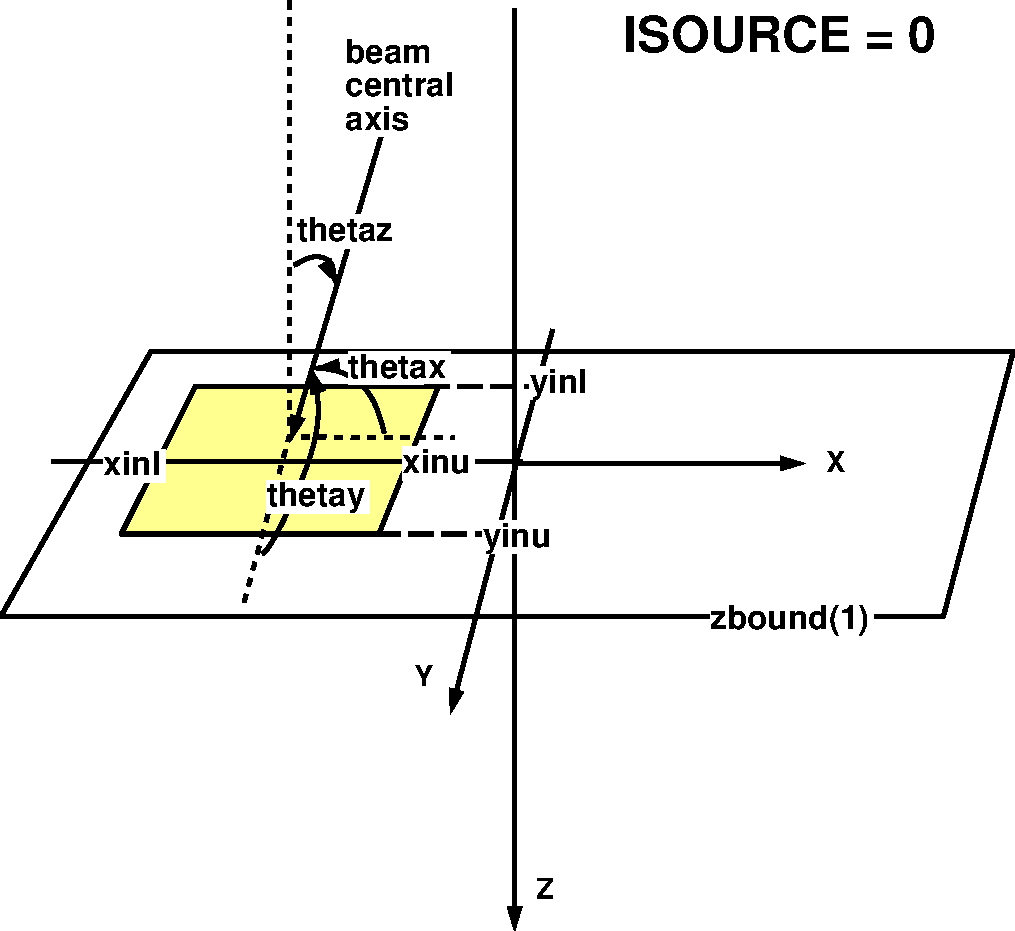
\includegraphics[height=12cm]{figures/src0}
\caption{Parallel rectangular beam (isource=0) showing the beam field, defined by
{\tt xinu}, {\tt xinl, yinu}, and {\tt yinl} on the phantom surface and the
beam directions, {\tt thetax}, {\tt thetay}, and {\tt thetaz}.
The angles {\tt thetax} and {\tt thetay} are relative to the positive x- and y-axes respectively,
while {\tt thetaz} is measured relative to the negative z-axis.}
\label{fig_src0}
\end{center}
\end{figure}
\indexm{xinl,xinu}
\indexm{yinl,yinu}
\indexm{thetax}
\indexm{thetay}
\indexm{thetaz}

\clearpage

\rfoot[]{}

\subsection{isource = 1: Parallel Rectangular Beam Incident from Any Direction}
\indexm{source routines!isource = 1}
\indexm{source routines!parallel any direction}

This uniform parallel rectangular beam may be incident from any direction. The input parameters are:

\begin{description}
\item [~~~~{\tt iqin}] Charge of the incident beam (-1: electron, 0: photon, 1: positron)
\indexm{iqin}
\item [~~~~{\tt isource}] = 1
\item [~~~~{\tt xiso/yiso/ziso}] x-, y-, z-coordinates of the isocenter.  The
isocenter is normally inside the phantom.
\indexm{xiso,yiso,ziso}

\item [~~~~{\tt theta}]   Angle between the +z direction and a line joining
the center of the beam where it strikes the phantom surface to the
isocenter.  In a polar coordinate system, this angle is known as the polar
angle and normally has a range 0-180 degrees.  Note that a centred beam
incident along the +z-axis (ie from the top) has {\tt theta}=180 degrees.
{\tt theta} is
not to be confused with {\tt thetaz} for isource=0, for which case {\tt
thetaz}=0 degrees to aim the source=0 beam along the +z-axis.
\indexm{thetaz}
\indexm{theta}


\item [~~~~{\tt phi}]      Angle  between the +x direction and the
projection on the x-y plane of the line joining the center of the beam on
the phantom surface to the isocenter on the xy plane.  In a polar
coordinate system, this angle is known as the azimuthal angle and normally
has a range 0-360 degrees.
\indexm{phi}

\item [{\tt xcol}/{\tt ycol}]  Total x- and y-widths of the beam on
the plane perpendicular to the beam direction, defined by the center of
the beam and the isocenter
\indexm{ycol}
\indexm{xcol}

\item [{\tt phicol}]  Angle by which the collimator is rotated in the
collimator plane perpendicular to the beam direction.  {\tt phicol} is
determined for {\tt theta}={\tt phi}=0.  The positive sense of rotation is
counterclockwise as one sights down the beam direction.  Note that the
effect of setting {\tt phicol}=90 degrees is the same as switching the
values of {\tt xcol} and {\tt ycol} when {\tt theta} and {\tt phi} are 0
or are both multiples of 90 degrees.
\indexm{theta}
\indexm{phicol}
\end{description}

\clearpage

\rfoot[{\sffamily \rightmark}]{{\sffamily \leftmark}}

\begin{figure}[htbp]
\begin{center}
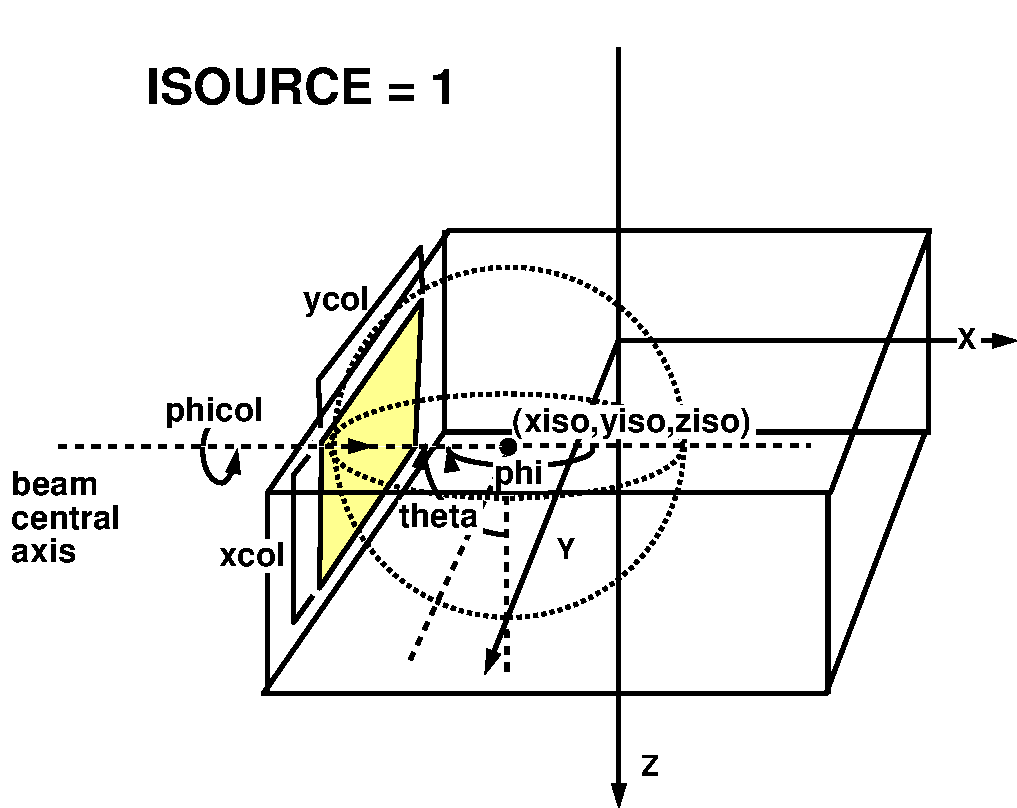
\includegraphics[width=16cm]{figures/src1}
\caption{Parallel rectangular beam incident from any direction (isource=1).  A
polar coordinate system is set up at the isocenter, (xiso,yiso,ziso).  The
position of the beam collimator is then defined using the angles, {\tt
theta} and {\tt phi}.  In the particular example shown in this figure,
with the beam incident on the centre of the negative Y face of the volume,
{\tt theta} is 90 degrees and {\tt phi} is 180 degrees.  The dimensions of
the rectangular collimator are given by {\tt xcol} and {\tt ycol}.  An
additional degree of freedom is available by allowing the collimator to
rotate in its own plane by angle {\tt phicol}.  Note that source 1 is
always incident right on the phantom surface (ie particles do not travel
through air to get to the phantom)}
\label{fig_src1}
\end{center}
\end{figure}
\indexm{xiso,yiso,ziso}
\indexm{theta}
\indexm{phi}
\indexm{phicol}

\clearpage

\subsection{isource = 2: Phase-Space Source Incident from Any Direction}
\label{source2sect}
\indexm{source routines!isource = 2}
\indexm{source routines!phase space}

This source uses a phase-space file generated during a BEAMnrc simulation at
any flat scoring plane of a linear accelerator geometry. A user can choose
any particular type of particles from the phase-space file and score dose
components using the {\tt LATCH} filter. The field size of the incident
\indexm{LATCH} beam can be reduced using the parameter {\tt BEAM\_SIZE}.
There is also a
\indexm{BEAM\_SIZE} parameter called {\tt ISMOOTH} which
can be set to 1 if one wants to shift
\indexm{ISMOOTH} the particles to
their symmetrical positions with respect to x- and y-axis in the
phase-space file for repeated use of these phase-space particles. For {\tt
ISMOOTH} = 0, no shift will be made when phase-space particles are
re-used.  {\tt LATCH} filter, {\tt BEAM\_SIZE} and {\tt ISMOOTH} are input
later in the file.
\indexm{re-use of phase space}

Input parameters for a phase-space source are:
\begin{description}
\item [~~~~{\tt iqin}] Charge of the incident beam (-1: electron, 0:
\indexm{iqin}
            photon, 1: positron, 2: all particle types)
\item [~~~~{\tt isource}] = 2
\item [~~~~{\tt xiso/yiso/ziso}] x-, y-, z-coordinates of the isocenter
\indexm{xiso,yiso,ziso}
                 (normally located within the phantom)
\item [~~~~{\tt theta}]   Same as for isource=1.
\indexm{theta}

\item [~~~~{\tt phi}]     Same as for isource=1.
\indexm{phi}
\item [~~~~{\tt dsource}]      For a BEAMnrc format phase space source, this
is the absolute distance from the isocenter to the
source center, which is, by definition, the origin of the phase-space
plane (origin may not even be in the beam).  For an IAEA format phase
space source, this is the distance from the isocentre to the primary
source ({\it i.e.} the source used to generate the phase space file), or
SAD.
\indexm{dsource}

\item [~~~~{\tt phicol}]  Angle by which the source is rotated in the
                     source plane perpendicular to the beam direction.
                     {\tt phicol} is determined for {\tt theta}={\tt phi}=0.
                     The positive sense of rotation is counterclockwise
                     as one sights down the beam direction.
\indexm{phicol}

\indexm{DBS}
\indexm{directional bremsstrahlung splitting}
\item [~~~~{\tt i\_dbs}] Set to 1 if the phase space source was generated
using directional bremsstrahlung splitting (DBS) in BEAM {\bf AND} you
wish to reject photons directed outside the splitting field (which will
all be fat).  Set to 0 otherwise.  Note that {\tt i\_dbs} is read in as
a real and converted to integer.
\indexm{i\_dbs}

\item [~~~~{\tt r\_dbs}] Radius (in cm) of the DBS splitting field in
the BEAMnrc simulation used to generate this source. Only needed if {\tt
i\_dbs} = 1.
\indexm{r\_dbs}

\item [~~~~{\tt ssd\_dbs}] SSD (in cm) where the DBS splitting field radius
was defined in the BEAMnrc simulation used to generate this source.
Only needed if {\tt i\_dbs} = 1.
\indexm{ssd\_dbs}

\item [~~~~{\tt z\_dbs}] Z value (in cm) in the BEAMnrc simulation
where this phase space source was scored.  This will be at the back of
a component module (CM).  Only needed if {\tt i\_dbs} = 1.
\indexm{{\tt z\_dbs} }

\item [~~~~{\tt e\_split}]  Number of times to split charged particles
as soon as they enter the phantom geometry.  Split particles have their
weight reduced by a factor of 1/{\tt e\_split}.  This is only used
in conjunction with photon splitting ({\tt n\_split}, see Section~\ref{nsplitsect}) and
prevents higher-weight contaminant electrons from compromising statistics
in photon beams.  For maximum efficiency, it is suggested that you
set {\tt e\_split}={\tt n\_split}, the photon splitting number.
\indexm{source 2!charged particle splitting}
\indexm{e\_split}

\indexm{{\tt FILNAM}}
\item [~~~~{\tt FILNAM}] The full name (including extension) of the phase space file
(including the directory path).  In the case of an IAEA-format phase space
source, the full name of the phase space data ({\tt .IAEAphsp}) file
\indexm{IAEA phase space source}
is input here.  The header ({\tt .IAEAheader}) file as assumed to exist
in the same directory.  For more information about IAEA-format date, see
the BEAMnrc Manual.

\end{description}

{\tt theta}, {\tt phi} and {\tt dsource} can be set to place the source
anywhere inside the phantom or the surrounding region; the medium and the
thickness of the surrounding region is input by the user.  Particles from
the phase space which are initially outside both the phantom and surrounding
region are terminated immediately.  If the medium of the surrounding
region is air, for example,  the phase-space particles will be transported
{\it properly} through air to the surface of the phantom. A particle
history is terminated if it is determined that the particle will not make
it to the phantom surface (the particle loses all its energy in the
surrounding region or it escapes through the outer boundaries of the
surrounding region).


Note that, for source 2, the user must set {\tt enflag} = 2 or 3, input
the \indexm{enflag}
mode of the phase-space file (0 or 2), and input the medium number and the
thickness for the surrounding region.  The user should also input the
phase-space file name after the above inputs.  These other inputs are
described in sections 5 and 6 below.  For more information related to
phase-space sources, see the section on phase-space files in the
BEAMnrc User's Manual
\cite{Ro04a}.

The value of {\tt phicol} must be set to 180 degrees in order for the X-Y
coordinates in a BEAMnrc-generated phase space source to map onto the
equivalent X-Y coordinates in DOSXYZnrc.  This is because of the general
coordinate transformation done going from BEAMnrc to DOSXYZnrc.

\subsubsection[DBS Inputs]{Inputs related to directional bremsstrahlung
splitting}
\label{i_dbs_sect}

\indexm{DBS}
\indexm{directional bremsstrahlung splitting}
\indexm{fat photons}
If you have used the directional bremsstrahlung splitting (DBS) variance
reduction technique (see the BEAMnrc User's Manual\cite{Ro04a} for more
details) to
generate the phase space source, then it is recommended that you use
the inputs {\tt i\_dbs}, {\tt r\_dbs}, {\tt ssd\_dbs} and {\tt z\_dbs} to
prevent unsplit, high-weight (``fat") photons which are outside the
splitting field from compromising your dose statistics.
{\tt r\_dbs} and {\tt ssd\_dbs} (the DBS splitting field radius and
SSD in cm) are available directly from the inputs for DBS in the BEAM
simulation, while {\tt z\_dbs} is simply the Z value at the back of the
component module (CM) in the BEAMnrc simulation in which this phase space source was scored.  If
{\tt i\_dbs} is set to 1, then before a photon is used in the DOSXYZnrc
simulation, it is projected along its trajectory from {\tt z\_dbs}
to {\tt ssd\_dbs} (we assume {\tt ssd\_dbs}$\geq${\tt z\_dbs}).  If it
falls outside {\tt r\_dbs} at {\tt ssd\_dbs}, then the photon is
not used in the DOSXYZnrc simulation.  In the context of the BEAM simulation
this photon will not have been split and will be fat (but this information
is not carried in the phase space file except indirectly because of the
larger weight which is not a unique specifier).  To be able to ignore these
fat photons and thereby increase the efficiency considerably, it is
important to ensure that the dose from the photons being ignored is
negligible. This can usually be arranged by making the splitting field big
enough.
\indexm{DBS}
\indexm{directional bremsstrahlung splitting}

Note that charged particles are not
rejected with this technique, which means that if you do not want fat charged
particles to compromise dose statistics (especially near the surface of a
phantom) then you must use the electron splitting option in DBS
(again, see the BEAMnrc User's Manual for more details).

\subsubsection{IAEA format phase space sources}
\label{src2iaeasect}
\indexm{source 2!IAEA format phase space file}
In the case of an IAEA format phase space source, the input, {\tt dsource} (see above), defines the distance
from the primary source ({\it i.e.} the source used to generate the phase space file) to the phantom
isocentre, or SAD.  This is because, unlike BEAMnrc format phase space files, the incident Z-position of
particles is available and read from either the phase space data (in the case of 3-D phase space files) or the header file
(in the case of planar phase space files, such as those scored by BEAMnrc).  The input value of {\tt dsource} is then
subtracted from this Z-position to give the distance along the beam axis from the phantom isocentre to the
particle incident position.

The ability of source 2 to automatically handle IAEA phase space files in which the Z-position for each
particle is scored (3-D data) is particularly useful in cases where the phase space data available for
an accelerator is scored on a non-planar surface (as is the case with the data that Varian has made
available for their TrueBeam accelerators) or when using 3-D phase space data scored by an upstream
DOSXYZnrc simulation (see Section~\ref{phspoutsect}).

\begin{figure}[htbp]
\begin{center}
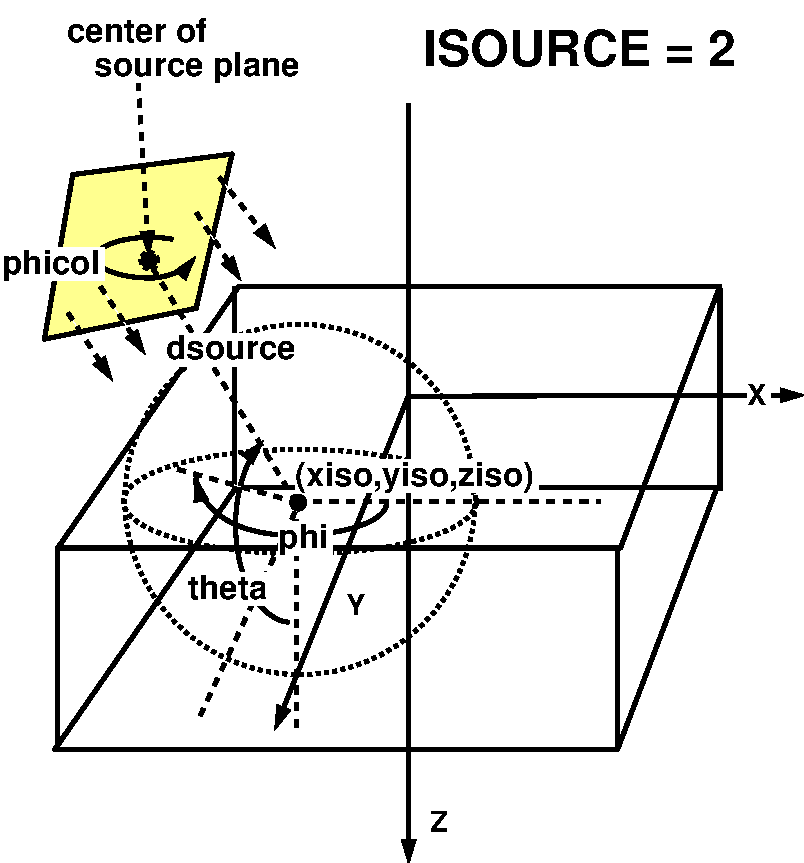
\includegraphics[width=14cm]{figures/src2}
\caption{Phase-space source incident from any direction (isource=2).
Similar to
source 1, a polar coordinate system is set up at the isocenter, (xiso,
yiso, ziso).  The position of the origin in the phase-space plane is then
defined by the angles {\tt theta} and {\tt phi}, and the distance from the
isocenter, {\tt dsource}.  The source can be rotated in its own plane
using the variable {\tt phicol}.  The figure shows that the source plane
does not necessarily have to be right against the surface of the phantom,
however it must be within the surrounding region specified by {\tt dsurround}
 (see section ~\ref{sec5}).}
\label{fig_src2}
\end{center}
\end{figure}
\indexm{dsource}
\indexm{phicol}
\indexm{theta}
\indexm{phi}
\indexm{xiso,yiso,ziso}
\indexm{dsurround}

\clearpage

\subsection{isource = 3: Point Source Rectangular Beam Incident from Front}
\indexm{source routines!isource = 3}
\indexm{source routines!point source rectangle}

The isotropically-radiating point source is placed on the Z-axis.  It is
assumed to be incident on the front surface of the phantom, but can be
placed any distance above the phantom.  The beam field can be asymmetric.

The input parameters for the point source are:
\begin{description}

\item [~~~~{\tt iqin}] Charge of the incident beam (-1: electron, 0:
\indexm{iqin}
                  photon, 1: positron)
\item [~~~~{\tt isource}] = 3
\item [~~~~{\tt xinl,xinu}] Lower and upper x-bounds of the field on the
\indexm{xinl,xinu}
          phantom surface
\item [~~~~{\tt yinl,yinu}] Lower and upper y-bounds of the field on the
\indexm{yinl,yinu}
                   phantom surface
\item [~~~~{\tt ssd}] Distance from the point source to the phantom surface (cm)
\indexm{ssd}
\end{description}

Note that, between the source and the phantom surface the medium is
assumed to be a vacuum for this source.

\begin{figure}[htbp]
\begin{center}
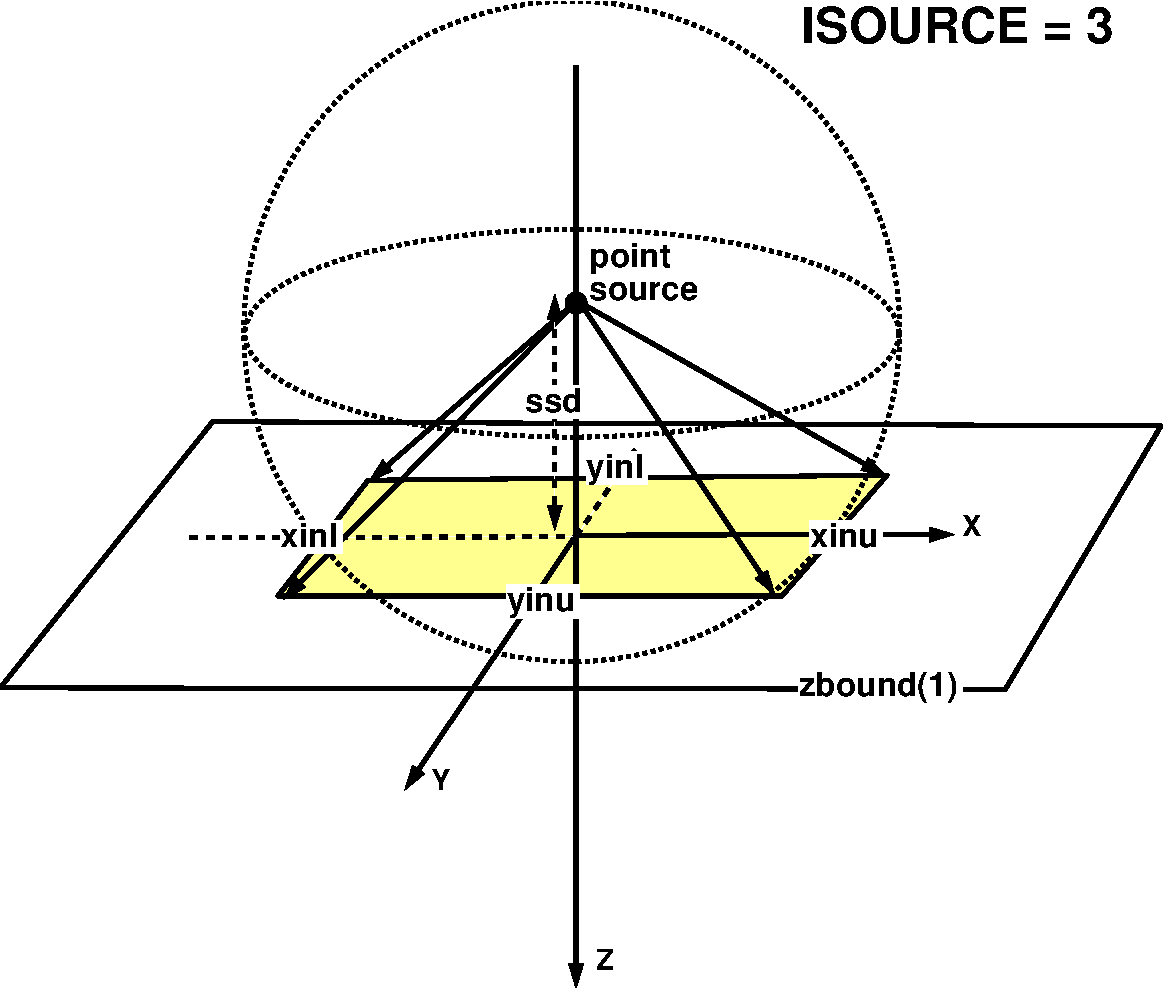
\includegraphics[height=11cm]{figures/src3}
\caption{Point source incident from the front (isource=3).  The
isotropically-radiating point source is located on the Z-axis at distance
ssd above the phantom.  The source is collimated to a rectangular field
defined by xinu, xinl, yinu, yinl on the phantom surface.}
\label{fig_src3}
\end{center}
\end{figure}
\indexm{xinl,xinu}
\indexm{yinl,yinu}

\clearpage


\subsection{isource = 4: Beam Characterization Model Incident
from Any Direction}
\indexm{source routines!isource = 4}
\indexm{source routines!beam characterization}

This source uses the beam characterization models created by BEAMDP from
phase space
data generated by BEAMnrc. This source consists of a variety of sub-sources
for different types of particles coming from different components of a
linear accelerator. Each sub-source has its own spectral and (planar)
fluence distributions and the correlation between the energy, position and
incident angle is retained by sampling the particle positions on the
sub-source (the surface of the component) and on the phase-place plane. A
beam model input file, generated by BEAMDP, is required by this source.
For more details about beam characterization models see the
BEAMnrc User's Manual and associated paper\cite{Ma95c,Ma97}.
\indexm{BEAMDP}

Apart from {\tt isource}, which must be set to 4, input parameters for source 4 are the same as for source 2:

\indexm{enflag}
Note this source requires {\tt enflag} = 4 and to input the beam model
input file name after the {\tt enflag} input. The field size of the
incident beam can be reduced using the parameter {\tt BEAM\_SIZE}.  These
inputs are described in sections 5 and 6 below.
\indexm{BEAM\_SIZE}

The default version of DOSXYZnrc does not include this source. In order to
use it you must recompile DOSXYZnrc using the instructions in
section~\ref{include4}. .

\clearpage

\rfoot[]{}

\subsection{isource = 6: Uniform Isotropically Radiating Parallelepiped
within DOSXYZnrc Volume}
\indexm{source routines!isource = 6}
\indexm{source routines!beam characterization}

This source allows the user to simulate a uniform isotropically radiating
rectangular volume (parallelepiped) within the DOSXYZnrc phantom.
The active volume is restricted to being completely contained within the
DOSXYZnrc phantom.  However, it can be shrunk to a point anywhere within the
phantom.

The input parameters for the uniform isotropically radiating parallelepiped:
\begin{description}

\item [~~~~{\tt iqin}] Charge of the incident beam (-1: electron, 0:
\indexm{iqin}
                  photon, 1: positron)
\item [~~~~{\tt isource}] = 6
\item [~~~~{\tt xinl,xinu}] Lower and upper x-bounds of the active volume (cm)
\indexm{xinl,xinu}
\item [~~~~{\tt yinl,yinu}] Lower and upper y-bounds of the active volume (cm)
\indexm{yinl,yinu}
\item [~~~~{\tt zinl,zinu}] Lower and upper z-bounds of the active volume (cm)
\indexm{zinl,zinu}
\end{description}

\begin{figure}[htbp]
\begin{center}
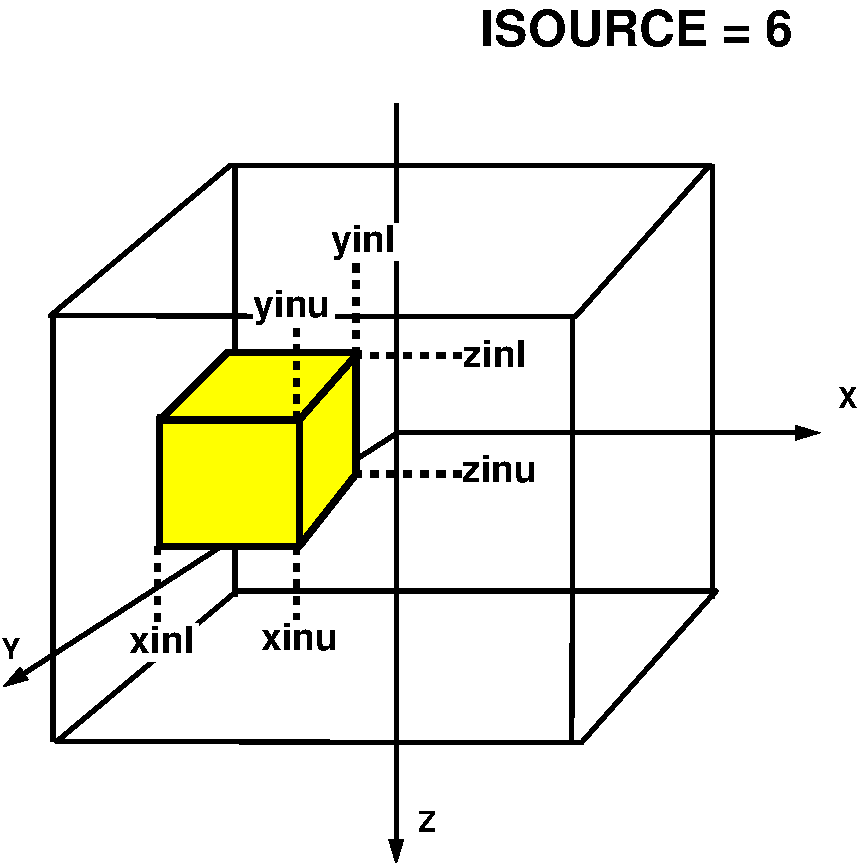
\includegraphics[height=11cm]{figures/src6}
\caption{Uniform isotropically radiating parallelepiped within DOSXYZnrc phantom
(isource=6).  The active volume, specified by {\tt xinl, xinu, yinl,
yinu, zinl, zinu}, must fit within the phantom.  The source can be shrunk
to a point within the phantom by setting {\tt xinu=xinl}, {\tt yinl=yinu}
and {\tt zinl=zinu}.}
\label{fig_src6}
\end{center}
\end{figure}
\indexm{xinl,xinu}
\indexm{yinl,yinu}
\indexm{zinl,zinu}

\clearpage

\subsection{isource = 7: Parallel Rectangular Beam Incident from Multiple Directions}
\label{source7_sec}
\indexm{source routines!isource = 7}
\indexm{source routines!parallel multiple directions}

This is a uniform parallel rectangular beam similar to source 1,
but incident from multiple, user-defined
directions (theta-phi pairs). The input parameters are:

\begin{description}
\item [~~~~{\tt iqin}] Charge of the incident beam (-1: electron, 0: photon, 1: positron)
\indexm{iqin}
\item [~~~~{\tt isource}] = 7
\item [~~~~{\tt xiso/yiso/ziso}] x-, y-, z-coordinates of the isocenter.  The
isocenter is normally inside the phantom.
\indexm{xiso,yiso,ziso}

\item [~~~~{\tt nang}]  The number of incident theta-phi pairs
or, if negative, then abs({\tt nang}) is the number of groups of
incident theta-phi pairs, where, within a group, all theta-phi pairs have
equal probability.  The incident angles theta and phi are defined the
same as they are in source 1.  Theta-phi pairs/groups are specified on
separate lines (see below).
\indexm{nang}
\indexm{theta-phi pairs}

\item [~~~~{\tt xcol}/{\tt ycol}]  Total x- and y-widths of the beam on
the plane perpendicular to the beam direction, defined by the center of
the beam and the isocenter
\indexm{ycol}
\indexm{xcol}

\item [~~~~{\tt phicol}]  Angle by which the collimator is rotated in the
collimator plane perpendicular to the beam direction.  {\tt phicol} is
defined the same way as in source 1.
\indexm{phicol}
\end{description}

And then, on the subsequent {\tt abs(nang)}  lines:\\

{\bf If {\tt nang} $>$ 0:}\\
~~~\\
For i=1,{\tt nang}: {\tt theta(i), phi(i), pang(i)}
\begin{description}
\item [~~~~{\tt theta(i)}]  Theta for pair i (degrees).
\item [~~~~{\tt phi(i)}]  Phi for pair i (degrees).
\item [~~~~{\tt pang(i)}] Probability of particle being incident at
                          Theta(i)-Phi(i).
\indexm{theta(i)}
\indexm{phi(i)}
\indexm{pang(i)}
\end{description}
{\bf If {\tt nang} $<$ 0:}\\
~~~\\
For i=1,-{\tt nang}: {\tt ivary(i), angfixed(i), angmin(i), angmax(i),
ngang(i), pgang(i)}
\begin{description}
\item [~~~~{\tt ivary(i)}] Set to 0 to vary phi in group i; Set to 1 to vary
theta in group i.
\item [~~~~{\tt angfixed(i)}] Fixed theta ({\tt ivary(i)}=0) or phi
({\tt ivary(i)}=1) in group i (degrees).
\item [~~~~{\tt angmin(i)}] Minimum varying phi ({\tt ivary(i)}=0) or
theta ({\tt ivary(i)}=1) in group i (degrees).
\item [~~~~{\tt angmax(i)}] Maximum varying phi ({\tt ivary(i)}=0) or
theta ({\tt ivary(i)}=1) in group i (degrees).
\item [~~~~{\tt ngang(i)}] Number of equally-spaced phi ({\tt ivary(i)}=0) or
theta ({\tt ivary(i)}=1) between and including {\tt angmin(i)} and
{\tt angmax(i)} in group i (Note that, since it includes
{\tt angmin(i)} and {\tt angmax(i)}, {\tt nang(i)} must be $\geq$ 2).
\item [~~~~{\tt pgang(i)}] Probability of particle being in group i.  Within
a group, all theta-phi pairs have equal probability.
\indexm{ivary(i)}
\indexm{angfixed(i)}
\indexm{angmin(i)}
\indexm{angmax(i)}
\indexm{ngang(i)}
\indexm{pgang(i)}
\end{description}

Note that the {\tt pang(i)} are automatically normalized.


\subsection{isource = 8: Phase-Space Source Incident from Multiple Directions}
\label{src8sect}
\indexm{source routines!isource = 8}
\indexm{source routines!phase space from multiple\\ directions}

This source is similar to source 2, except that it is incident from
multiple, user-defined directions (theta-phi pairs).

Input parameters for source 8 are:
\begin{description}
\item [~~~~{\tt iqin}] Charge of the incident beam (-1: electron, 0:
\indexm{iqin}
            photon, 1: positron, 2: all particle types)
\item [~~~~{\tt isource}] = 8
\item [~~~~{\tt xiso/yiso/ziso}] x-, y-, z-coordinates of the isocenter
\indexm{xiso,yiso,ziso}
                 (normally located within the phantom)

\item [~~~~{\tt nang}]  The number of incident theta-phi pairs
or, if negative, then abs({\tt nang}) is the number of groups of
incident theta-phi pairs, where, within a group, all theta-phi pairs have
equal probability.  The incident angles theta and phi are defined the
same as they are in source 2.  Theta-phi pairs/groups are specified the
same way as they are in source 7 (see section~\ref{source7_sec} above).
\indexm{nang}
\indexm{theta-phi pairs}

\item [~~~~{\tt dsource}]      For BEAMnrc phase space files, this
is the absolute distance from the isocenter to the
source center, which is, by definition, the origin of the phase-space
plane (origin may not even be in the beam).  For IAEA phase space files, this
is the primary source to isocentre distance (SAD).
\indexm{dsource}

\item [~~~~{\tt phicol}]  Angle by which the source is rotated in the
                     source plane perpendicular to the beam direction.
                     {\tt phicol} is determined for {\tt theta}={\tt phi}=0.
                     The positive sense of rotation is counterclockwise
                     as one sights down the beam direction.
\indexm{phicol}
\indexm{DBS}
\indexm{directional bremsstrahlung splitting}
\item [~~~~{\tt i\_dbs}] Set to 1 if the phase space source was generated
                     using directional bremsstrahlung splitting (DBS) in
                     BEAMnrc {\bf AND} you wish to reject photons directed outside
                     the splitting field (which will all be fat).  Set to 0 otherwise.
		Note that {\tt i\_dbs} is read in as a real and converted to integer.
\indexm{i\_dbs}
\item [~~~~{\tt r\_dbs}] Radius (in cm) of the DBS splitting field in
the BEAMnrc simulation used to generate this source. Only needed if {\tt
i\_dbs} = 1.  \indexm{r\_dbs}

\item [~~~~{\tt ssd\_dbs}] SSD (in cm) where the DBS splitting field
radius was defined in the BEAMnrc simulation used to generate this
source. Only needed if {\tt i\_dbs} = 1.  \indexm{ssd\_dbs}

\item [~~~~{\tt z\_dbs}] Z value (in cm) in the BEAMnrc simulation
where this phase space source was scored.  This will be at the back of
a component module (CM). Only needed if {\tt i\_dbs} = 1.  \indexm{{\tt
z\_dbs} }

\indexm{e\_split}
\indexm{source 8!charged particle splitting}
\item [~~~~{\tt e\_split}] Number of times to split charged particles
as soon as they enter the phantom.  The weight of split particles
is reduced by a factor of 1/{\tt e\_split}.  This is used in
conjunction with photon splitting (input variable {\tt n\_split}, see
Section~\ref{nsplitsect}) to prevent higher-weight contaminant electrons
from compromising dose statistics.  For optimum efficiency,
set {\tt e\_split}={\tt n\_split}.

\indexm{{\tt FILNAM}}
\item [~~~~{\tt FILNAM}] The full name (including extension) of the phase space
file
(including the directory path).  See the description of
source 2 (Section~\ref{source2sect}) for more details.
\end{description}
An example may help illustrate this input.  The following input:
\typeout{}
\typeout{*******Example end of 4.9 has two extra variables??  *************}
\typeout{*******Example end of 4.9 has two extra variables??  *************}
\typeout{*******Example end of 4.9 has two extra variables??  *************}
\typeout{}
\begin{verbatim}
0, 8, 0.0, 0.0, 0.0, -1.0, 80.0, 90.0, 0.0, 0.0, 0, 0.0, 0.0, 0.0
1, 90.0, 0.0, 356.40, 100, 1.0
\end{verbatim}
is for source 8. The phase space file rotates about the isocenter at
(0,0,0). The centre of the phase-space is 80 cm from the isocenter and the
collimator angle is 90 degrees.
The -1.0 indicates there is only one group of angles. The 1 at the start of
the second line tells us that phi is fixed (at 90 degrees)
and that theta is varying, in
this case in 100 discrete steps between 0 and 356.4 degrees with equal
intensity at each angle.  In this example, {\tt i\_dbs} is set to 0, indicating
that either directional bremsstrahlung splitting (DBS) was not used in the
BEAMnrc simulation that generated this source or else the user does not wish
to reject high-weight (``fat") photons created by DBS.

For more information on how to use the inputs {\tt i\_dbs},
{\tt r\_dbs}, {\tt ssd\_dbs} and {\tt z\_dbs} see section~\ref{source2sect}
on source 2 above.

Similar to source 2, source 8 automatically handles IAEA format phase space sources
with Z-position scored for each particle (3-D phase space).

\subsection{isource = 9: BEAM Treatment Head Simulation Incident from Any
Direction}
\label{src9sect}
\indexm{source routines!isource = 9}
\indexm{source routines!full BEAM simulation}

This source uses particles sampled from a BEAM simulation running
concurrently with the DOSXYZ
\indexm{BEAM accelerator code}
simulation.  The BEAM accelerator code must be compiled as a shared
library (existing in directory {\tt \$EGS\_HOME/bin/config}, where
{\tt config} is the name of your configuration) and must be supplied
with its own input file and pegs data file.  More details about this
are given below.  Source particles for DOSXYZ are then sampled from what
would be the scoring plane during a normal run of the BEAM accelerator.
Thus, this source is similar to {\tt isource}=2 (full phase space file)
without the need to store a phase space file.

\indexm{C/C++ compiler}
\indexm{config.conf file}
\indexm{BEAMLIB\_OBJECTS}
\indexm{BEAMLIB\_EXTRA\_LIBS}
Note that if you are running on Unix/Linux you must have a working C/C++
compiler to use this source and the file
{\tt \$HEN\_HOUSE/specs/config.conf} ({\it i.e.} file {\tt \$EGS\_CONFIG})
must have the variable
{\tt BEAMLIB\_OBJECTS} set to
\indexm{load\_beamlib.o}
{\tt \$(HEN\_HOUSE)lib/\$(my\_machine)/load\_beamlib.o} and\\
{\tt BEAMLIB\_EXTRA\_LIBS} set to {\tt $-$ldl}.
If you have installed EGSnrcMP on a Unix/Linux system with a working C/C++
compiler, the installation will automatically compile the C code
\indexm{load\_beamlib.c}
{\tt \$HEN\_HOUSE/cutils/load\_beamlib.c} to create
{\tt load\_beamlib.o}, and {\tt BEAMLIB\_OBJECTS} and
{\tt BEAMLIB\_EXTRA\_LIBS} will
automatically be set to their proper values.  Otherwise
{\tt BEAMLIB\_OBJECTS} and
{\tt BEAMLIB\_EXTRA\_LIBS} will remain
undefined (ie definitions left blank).

If you are running on Windows, then there is no requirement to have
a working C/C++ compiler to use this source.  In this case, the installation
automatically sets {\tt BEAMLIB\_OBJECTS} in
{\tt \$HEN\_HOUSE/specs/config.conf} to
\indexm{load\_beamlib.obj}
{\tt \$(HEN\_HOUSE)lib/\$(my\_machine)/load\_beamlib.obj}, where
{\tt load\_beamlib.obj} is a precompiled version of {\tt load\_beamlib.o}
included with the installation.  {\tt BEAMLIB\_EXTRA\_LIBS} does not
need to be defined and is left
blank.  See the BEAMnrc Manual\cite{Ro04a} for more information about
{\tt config.conf} files.

Similar to {\tt isource = 2}, you can select particles from the BEAM simulation
\indexm{LATCH}
to use based on their charge and/or {\tt LATCH} values.   You can also
select the maximum size of the BEAM field considered using the
\indexm{BEAM\_SIZE}
{\tt BEAM\_SIZE} input (discussed in more detail in its own section below).

Input parameters for source 9 are:
\begin{description}
\item [~~~~{\tt iqin}] Charge of the incident beam (-1: electron, 0:
\indexm{iqin}
            photon, 1: positron, 2: all particle types)
\item [~~~~{\tt isource}] = 9
\item [~~~~{\tt xiso/yiso/ziso}] x-, y-, z-coordinates of the isocenter
\indexm{xiso,yiso,ziso}
                 (normally located within the phantom)
\item [~~~~{\tt theta}]   Same as for isource=2.  Recall that, for a
beam coming down from the top of the phantom, {\tt theta}=180 degrees.
\indexm{theta}

\item [~~~~{\tt phi}]     Same as for isource=2.
\indexm{phi}
\item [~~~~{\tt dsource}]      Absolute distance from the isocenter to the
centre of the source plane, which is, by definition, the origin of the
scoring plane in the BEAM simulation.
\indexm{dsource}

\item [~~~~{\tt phicol}]  Angle by which the source is rotated about the
                     BEAM central axis.
                     {\tt phicol} is determined for {\tt theta}={\tt phi}=0.
                     The positive sense of rotation is counterclockwise
                     for {\tt theta}=0.  If {\tt theta}=180 degrees
                     (ie beam coming down from the top), then
                     {\tt phicol} must be set to 180 degrees to have the
                     BEAM x-y coordinates match the DOSXYZ x-y coordinates.
\indexm{phicol}

\indexm{DBS}
\indexm{directional bremsstrahlung splitting}
\item [~~~~{\tt i\_dbs}] Set to 1 if directional bremsstrahlung splitting
(DBS) is being used in the BEAM simulation {\bf AND} you wish to reject
fat photons falling outside the DBS splitting field.  This is recommended
so that the fat photons do not compromise dose statistics.  Note that,
with {\tt isource}=9, we have direct access to the BEAM stack variable
({\tt IPHAT}) indicating whether a photon is fat or not, thus we do not
need to reconstruct the DBS splitting field using the additional
inputs {\tt r\_dbs}, {\tt ssd\_dbs} and {\tt z\_dbs} required in
source 2.
\indexm{i\_dbs}

\item [~~~~{\tt e\_split}]  Number of times to split charged particles
as soon as they enter the phantom geometry.  Split particles have their
weight reduced by a factor of 1/{\tt e\_split}.  This is only used
in conjunction with photon splitting ({\tt n\_split}, see Section~\ref{nsplitsect}) and
prevents higher-weight contaminant electrons from compromising statistics
in photon beams.  For maximum efficiency, it is suggested that you
set {\tt e\_split}={\tt n\_split}, the photon splitting number.
\indexm{source 9!charged particle splitting}
\indexm{e\_split}

In addition to the above inputs, the user must input the following
information, all on one line, separated by commas. This line of input
follows the {\tt enflag} input line, {\it i.e.} the second line after the
above input.

\indexm{the\_beam\_code}
\item [~~~~{\tt the\_beam\_code}]  The name of the BEAM accelerator
simulation (ie {\tt BEAM\_accelname}).  This code must have been compiled as
a shared library that exists in your\\ {\tt \$EGS\_HOME/bin/config}
directory.  More information
on compiling a BEAM code as a library is given below.

\indexm{the\_input\_file}
\item [~~~~{\tt the\_input\_file}]  The input file to use for the BEAM
simulation (no {\tt .egsinp} extension).  This file must exist in
your {\tt \$EGS\_HOME/BEAM\_accelname} directory (ie the accelerator
directory).  In the BEAM input file, you must define a single scoring plane
in the accelerator, where
the source particles will be sampled, and the BEAM input
parameter {\tt IO\_OPT} must be set to output a phase space file at
this scoring plane.  See the BEAMnrc Manual\cite{Ro04a} for more information
about scoring planes and {\tt IO\_OPT}.  {\tt the\_input\_file} will
define a value of {\tt NCASE} (no. of histories) for the BEAM simulation,
but this is ignored and the BEAM simulation will always run until
{\tt NCASE} for the DOSXYZ simulation is reached.
\indexm{IO\_OPT}
\indexm{NCASE}

\item [~~~~{\tt the\_pegs\_file}]  The pegs data to be used in the BEAM
\indexm{the\_pegs\_file}
simulation (no {\tt .pegs4dat} extension).  This file must exist in
either {\tt \$HEN\_HOUSE/pegs4/data} or
your\\ {\tt \$EGS\_HOME/pegs4/data} directory.

\end{description}

A graphical representation of source 9 is similar to that of
source 2 shown in Figure~\ref{fig_src2}.  In both sources, the
``source plane'' is the scoring plane in the BEAM simulation, but in source 9
particles are sampled as soon as they cross the scoring plane rather than
stored in a phase space file for later use.  Note that the BEAM central
axis points from the origin of the source plane to the isocenter.

Similar to source 2, {\tt theta}, {\tt phi} and {\tt dsource}
can be set to place the source
plane anywhere inside the phantom or the surrounding region; the medium and the
thickness of the surrounding region are input by the user.  Particles
initially falling outside both the phantom and surrounding
region are terminated immediately. A particle history is terminated if it
is determined that the particle will not make
it to the phantom surface (the particle loses all its energy in the
surrounding region or it escapes through the outer boundaries of the
surrounding region).

The user must also set {\tt enflag} = 2 or 3
the \indexm{enflag}
and input the medium number and the
thickness for the surrounding region.
These inputs are described in sections 5 and 6 below.

\subsubsection[Compiling a BEAM library]{Compiling a BEAM code as
a shared library}
\label{make_library_sect}
\indexm{BEAM shared library}

In order to compile your BEAM accelerator code, {\tt BEAM\_accelname}, as
a shared library, you must already have built the code and created your
\indexm{beam\_build}
directory {\tt \$EGS\_HOME/BEAM\_accelname} using the {\tt beam\_build}
tool.  Building a BEAM code is discussed in detail in the BEAM Manual\cite{Ro04a}.
Of course, if you have already been running {\tt BEAM\_accelname} as a
regular BEAM simulation, then the code will have already been built and
{\tt \$EGS\_HOME/BEAM\_accelname} will exist.  To compile the code as a
shared library, go into your directory \\{\tt \$EGS\_HOME/BEAM\_accelname}
and type:
\indexm{make!BEAM shared library}
\begin{verbatim}
make library
\end{verbatim}
\indexm{BEAM shared library!naming scheme}
If you are using a Unix/Linux system, this will create the
library {\tt libBEAM\_accelname.so}.  On a Windows system, the
library will be named {\tt BEAM\_accelname.dll}.  The library will
automatically be copied to your directory {\tt \$EGS\_HOME/bin/config},
where {\tt config} is the name of your configuration
(e.g. {\tt gcc}, {\tt win2k}, {\tt pgf77}, etc).  See the BEAM Manual for the
differences between the codes concatenated to create a BEAM library and those
used for a standard BEAM accelerator simulation.

\indexm{{\tt libg2c.a}}
In previous versions of BEAMnrc, the library {\tt libg2c.a} was required
when compiling shared library sources on Unix/Linux to avoid confusion of
Fortran units between DOSXYZnrc (the driving code) and BEAMnrc.  Recently,
however, the opening of files in BEAMnrc has been recoded so that only
available Fortran units are used.  This solves the problem of confusion
between Fortran units and eliminates the need for the {\tt libg2c.a}
\indexm{{\tt gfortran}}
library (which caused problems with the {\tt gfortran} compiler).

\indexm{the\_beam\_code}
Recall that when entering the input parameter {\tt the\_beam\_code},
specifying the BEAM simulation to use, you
simply use {\tt BEAM\_accelname}, omitting
the {\tt lib} prefix (in the case of a Unix/Linux library) and
the {\tt .so} or {\tt .dll} extension of the library.

\subsubsection[Efficiency of BEAMnrc simulation source vs. phase space source]
{Efficiency of BEAMnrc simulation source vs. a phase space source}
\indexm{BEAMnrc simulation source!efficiency vs. phase space source}

A BEAMnrc source has the obvious advantage over a phase space source
in that intermediate phase space data need not be stored.  For many
calculations with reasonable precision, this can save tens of
GBytes of disk storage space.  In general, the tradeoff will be a
reduced simulation efficiency, due to the extra
time required to perform a full accelerator simulation to generate
source particles.

Recent research\cite{KW06} has shown, however, that
by using variance reduction techniques in the BEAMnrc simulation
source and in the DOSXYZnrc calculation, the efficiencies of photon
beam dose calculations using BEAMnrc simulation sources can be maximized
so that they are only 3--13\% (depending on beam energy, field size and
phantom voxel size) lower than the peak efficiencies with the equivalent
phase space sources.  The variance reduction techniques required are
directional bremsstrahlung splitting (DBS--see Ref\cite{Ka04a}
and Section 6.3.4 in the BEAMnrc Manual) to maximize the efficiency
of photon production in the BEAMnrc simulation source in conjunction
with
photon splitting ({\tt n\_split}--see Section~\ref{nsplitsect}) to
maximize the efficiency of the DOSXYZnrc calculation.  Efficiencies
quoted for phase space sources include the time required to transport
particles through the accelerator jaws (from ``fixed'' phase space data
collected above the jaws) to generate the source, but even if this
time is omitted, the peak efficiencies with BEAMnrc simulation sources
are only 5--30\% lower than those with phase space sources.

\subsection{isource = 10: Full BEAMnrc Treatment Head Simulation Incident from Multiple Directions}
\indexm{source routines!isource = 10}
\indexm{source routines!BEAMnrc simulation source from\\ multiple directions}

This source is similar to source 9, except that it is incident from
multiple, user-defined directions (theta-phi pairs).

Inputs for source 10 are:
\begin{description}
\item [~~~~{\tt iqin}] Charge of the incident beam (-1: electron, 0:
\indexm{iqin}
            photon, 1: positron, 2: all particle types)
\item [~~~~{\tt isource}] = 10
\item [~~~~{\tt xiso/yiso/ziso}] x-, y-, z-coordinates of the isocenter
\indexm{xiso,yiso,ziso}
                 (normally located within the phantom)

\item [~~~~{\tt nang}]  The number of incident theta-phi pairs
or, if negative, then abs({\tt nang}) is the number of groups of
incident theta-phi pairs, where, within a group, all theta-phi pairs have
equal probability.   Same as for source 8 (see Section~\ref{src8sect} above
for more details).
\indexm{nang}
\indexm{theta-phi pairs}

\item [~~~~{\tt dsource}] Absolute distance from the isocenter to the
centre of the source plane.  Same as for source 9 (Section~\ref{src9sect}).
\indexm{dsource}

\item [~~~~{\tt phicol}] Angle by which the source is rotated about the
                     BEAM central axis.  Same as for source 9 (Section~\ref{src9sect}).
\indexm{phicol}

\indexm{DBS}
\indexm{directional bremsstrahlung splitting}
\item [~~~~{\tt i\_dbs}] Set to 1 if directional bremsstrahlung splitting
(DBS) is being used in the BEAM simulation {\bf AND} you wish to reject
fat photons falling outside the DBS splitting field so that they do not
compromise dose statistics.  Same as for source 9 (Section~\ref{src9sect}).
\indexm{i\_dbs}

\item [~~~~{\tt e\_split}]  Number of times to split charged particles
as soon as they enter the phantom geometry.  This is only used
in conjunction with photon splitting ({\tt n\_split}$>$1).
Same as for source 9 (Section~\ref{src9sect}).
\indexm{source 10!charged particle splitting}
\indexm{e\_split}

\indexm{the\_beam\_code}
\item [~~~~{\tt the\_beam\_code}]  The name of the BEAM accelerator
simulation (ie {\tt BEAM\_accelname}).  Same as for source 9 (Section~\ref{src9sect}).

\indexm{the\_input\_file}
\item [~~~~{\tt the\_input\_file}]  The input file to use for the BEAM
simulation (no {\tt .egsinp} extension).  Same as for source 9.

\item [~~~~{\tt the\_pegs\_file}]  The pegs data to be used in the BEAM
\indexm{the\_pegs\_file}
simulation (no {\tt .pegs4dat} extension).  Same as for source 9.

\end{description}

For an example of how the theta-phi pairs are specified, see the
description at the bottom of Section~\ref{src8sect} above.

Note that, similar to source 9, the user must also set {\tt enflag} = 2 or 3 \indexm{enflag} and input the medium number
and the thickness for the surrounding region. These inputs are described in sections 5 and 6 below.

\subsection{isource = 20: Synchronized phase space source}
\label{src20sect}
\indexm{source routines!isource = 20}
\indexm{source routines!Simulation through moving MLC}
\indexm{source routines!synchronized phase space source}

This source greatly enhances the capabilities of the phase space source incident from multiple directions (isource=8).
Source 20 was developed by Lobo and Popescu\cite{LP10} to allow the user to simulate continuous motion of the phase space
source relative to the DOSXYZnrc phantom over specified ranges of incident
directions, SSD's and isocentre coordinates.  Moreover, the source allows
the user to interpose a geometry, generated using either a BEAM accelerator or a non-EGSnrc code (likely simulating
an MLC geometry) compiled as a shared library, between the source plane and the DOSXYZnrc phantom.  In the case of a BEAM shared library, the source
parameters (range of incident directions, SSD's, isocentres) can be synchronized with the field settings of any synchronized
component modules (see the BEAMnrc Manual\cite{Ro09}).

The geometrical parameters controlling the orientation of the source plane relative to the DOSXYZnrc phantom
have the same definition as those for sources 2, 8, 9 and 10 and are shown in Figure~\ref{fig_src2}.

Input parameters for source 20 are:

\begin{description}
\item [~~~~{\tt iqin}]
\indexm{iqin}
Charge of the incident beam (-1: electron, 0: photon, 1: positron, 2: all particle types)
\item [~~~~{\tt isource}] = 20
\item [~~~~{\tt nset}]
\indexm{nset}
\indexm{\$MXANG}
The number of control points.  Control points define the beginning and end points of ranges of incident direction angles, SSD's and isocentre coordinates over which continuous motion of the source is simulated
(see below).  {\tt nset} must be in the range 2 $\leq$ {\tt nset} $\leq$ {\tt \$MXANG}, where {\tt \$MXANG} is defined in
the file\\ {\tt \$EGS\_HOME/dosxyznrc/dosxyznrc\_user\_macros.mortran}.
\item [~~~~{\tt i\_dbs}]
\indexm{i\_dbs}
Set to 1 if the phase space source was generated using directional bremsstrahlung splitting (DBS) in BEAM and you wish
to reject photons directed outside the splitting field (which will all be fat). Set to 0 otherwise. Note that
{\tt i\_dbs} is read in as a real and converted to integer.
\item [~~~~{\tt r\_dbs}]
\indexm{r\_dbs}
Radius (in cm) of the DBS splitting field in the BEAM simulation used to generate this source. Only needed if {\tt i\_dbs}=1.
\item [~~~~{\tt  ssd\_dbs}]
\indexm{ssd\_dbs}
SSD (in cm) where the DBS splitting field radius was defined in the BEAM simulation used to generate this source. Only needed if
{\tt i\_dbs} = 1.
\item [~~~~{\tt z\_dbs}]
\indexm{z\_dbs}
Z value (in cm) in the BEAM simulation where this phase space source was scored. This will be at the back of a component module (CM). Only needed if {\tt i\_dbs} = 1.
\item [~~~~{\tt e\_split}]
\indexm{e\_split}
Number of times to split charged particles as soon as they enter the phantom geometry. Split particles have their weight reduced by a factor of 1/{\tt e\_split}. This is only used in conjunction with photon splitting ({\tt n\_split}, see Section 8.16) and prevents higher-weight contaminant electrons from compromising statistics in photon beams. For maximum efficiency, it is suggested that you set {\tt e\_split=n\_split}, the photon splitting number.
\item [~~~~{\tt i\_muidx\_out}]
\indexm{i\_muidx\_out}
Set to 1 to include the fractional monitor unit index, {\tt MU}, associated with each particle in IAEA format phase
space output for particles leaving the phantom geometry.  Note that phase space data is not output at all
unless
\indexm{i\_phsp\_out}
{\tt i\_phsp\_out}, the input parameter in the main code controlling phase space output, is set to 1 or 2.
If {\tt MU} is included in the phase space output, then phase space data has a time dimension and is considered 4-D.
Scoring of {\tt MU} allows synchronization between the DOSXYZnrc simulation generating the file and any
downstream simulations--such as BEAMnrc simulations with synchronized component modules--using the file as
a source. See Section~\ref{phspoutsect} for a description of DOSXYZnrc phase space output.
\item [~~~~{\tt calflag}]
\indexm{calflag}
\indexm{NRCYCL}
Set to 1 to skip the calibration run through a BEAM shared library geometry between the source plane and
the phantom. The number of times to recycle each source particle before proceeding to the next one,
{\tt NRCYCL}, will then not take into account the ratio of the number of particles emerging from the
library geometry to the number of incident particles (survival ratio).  The default is to do the calibration run if a BEAM shared library geometry is present.
\end{description}

For i=2,...,{\tt nset} (the no. of control points), the following parameters are entered:
\begin{description}
\item[~~~~{\tt xiso(i)/yiso(i)/ziso(i)}]
\indexm{xiso,yiso,ziso}
x-, y-, z-coordinates of the isocenter.
\item[~~~~{\tt theta(i)}]
\indexm{theta(i)}
Angle of line connecting phase space plane to isocentre relative to the +Z axis.
\item[~~~~{\tt phi(i)}]
\indexm{phi(i)}
Angle of line connecting phase space plane to isocentre relative to the +X axis.
\item[~~~~{\tt phicol(i)}]
\indexm{phicol(i)}
2D Angle of rotation of the phase space plane about its own origin.
\item[~~~~{\tt dsource(i)}]
\indexm{dsource(i)}
The distance from the centre of the phase space plane to the isocentre except when an IAEA format phase space source
is used, in which case input the distance from the primary BEAM source to the isocentre (SAD).  When an IAEA phase space
source is used, the distance from the phase space plane to the isocentre is calculated using the Z position of
the phase space plane read in from the IAEA header file.
\item[~~~~{\tt muIndex(i)}]
\indexm{muIndex(i)}
A monitor unit index in the range $[$0,1$]$ defining the fraction of the total number of incident particles
delivered up to control point i.
Note that {\tt muIndex(i)} $\geq$ {\tt muIndex(i-1)}. Also note that for correct selection of the range
of incident source parameters, {\tt muIndex(i)=0.0} and {\tt muIndex(nset)=1.0}.  See below for more information
on how {\tt muIndex} is used to sample from a range of incident source parameters.
\end{description}
End of inputs required for each control point.

\begin{description}
\item[~~~~{\tt the\_shared\_lib}]
\indexm{the\_shared\_lib}
The name of the BEAM accelerator code or non-EGSnrc MLC simulation code compiled as a
shared library (See below for more information).  Leave this blank if there is no geometry interposed between the
phase space source and the DOSXYZnrc phantom.  This code must have been compiled as a shared library
({\it e.g.} {\tt libBEAM\_accelname.so} if a BEAM accelerator compiled on Unix/Linux) and exist in directory
{\tt \$EGS\_HOME/bin/config}, where {\tt config} is your configuration name.
\item[~~~~{\tt FILNAM}]
\indexm{FILNAM}
The full name (including directory path and file extension) of the phase space source.
\item[~~~~{\tt the\_input\_file}]
\indexm{the\_input\_file}
Input file for the BEAM or non-EGSnrc code defining the shared library geometry interposed between the
phase space source and the DOSXYZnrc phantom.  For a BEAM shared library, this input file must exist in
{\tt \$EGS\_HOME/BEAM\_accelname}   In the case of a BEAM shared library, this file must specify phase space
output at the bottom of the accelerator.
\end{description}

\indexm{MU\_RND}
\indexm{Source 20!Example control point settings}
Prior to each incident particle (Note: not necessarily a statistically-independent primary history)
a random number, {\tt MU\_RND}$\in[$0,1$]$, which can be thought of as a fractional monitor unit, is compared to the {\tt muIndex(i)} of the control points
to determine the incident geometrical parameters.  If source 20 is being run through a BEAM shared library geometry which has
synchronized component modules, such as SYNCJAWS and/or SYNCVMLC (See the BEAMnrc Users Manual\cite{Ro09}), then
the value of {\tt MU\_RND} is passed to BEAM from DOSXYZnrc (more on this below).
If {\tt muIndex(i-1)}$\leq${\tt MU\_RND}$<${\tt muIndex(i)}
then the parameters determining the orientation of the source plane are interpolated
between control points i-1 and i using:

\begin{equation}
{\tt PARAM}={\tt PARAM(i-1)}+\frac{\left[{\tt PARAM(i)}-{\tt PARAM(i-1)}\right]}
{\left[{\tt muIndex(i)}-{\tt muIndex(i-1)}\right]}\left[{\tt MU\_RND}-{\tt muIndex(i-1)}\right]
\end{equation}

Where {\tt PARAM} is the value of the source parameter ({\tt xiso}, {\tt yiso}, {\tt ziso}, {\tt theta}, {\tt phi}, etc) used in the simulation, and {\tt PARAM(i)} and {\tt PARAM(i-1)} are its values defined at control points i and i-1, respectively.
Thus, source parameters are evenly distributed between control points i-1 and i.

The generation of a new value of {\tt MU\_RND} for each incident particle means that particles in the phase space source arising
from the same primary history will be incident from different source orientations.  This was implemented to ensure adequate sampling
of source positions even in cases where where relatively few primary histories are represented in the phase space source
({\it i.e.} if the BEAM simulation used to generate the source used directional bremsstrahlung splitting with a high
splitting number).  Note, however, that regardless of how spatially well-sampled a dose distribution is, its uncertainty is
limited by the number of primary histories simulated.

An simple example input segment for {\tt nset}=7 is:

\begin{verbatim}
0, 0, -9, 90, 0, 0, 15, 0
0, 0, -9, 90, 360, 0, 15, 0.1
0, 0, -5, 90, 0, 45, 15, 0.1
0, 0, -5, 90, 360, 45, 15, 0.5
0, 0, 5, 90, 0, 90, 15, 0.5
0, 0, 5, 90, 360, 90, 15, 0.9
0, 0, 9, 90, 360, 135, 15, 1.0
\end{verbatim}

This sample input defines
four distinct ranges of incident source parameters:

\begin{enumerate}
\item The first two control points ({\tt muIndex(1)}=0.0, {\tt muIndex(2)}=0.1) define 10\% of incident particles
with ({\tt xiso, yiso, ziso})=(0, 0, -9), {\tt theta}=90$^o$ (i.e. incident
from the side of the phantom), {\tt phi} evenly distributed over $[$0,360$^o]$ (i.e. circling the entire phantom in the X-Y plane), {\tt phicol}=0$^o$, and {\tt dsource}=15 cm.
\item Control points 3 and 4, with {\tt muIndex(3)}=0.1 and {\tt muIndex(4)}=0.5, define 40\% of incident particles with
({\tt xiso, yiso, ziso})=(0, 0, -5), {\tt theta}=90$^o$, {\tt phi} evenly distributed over $[$0,360$^o]$, {\tt phicol}=45$^o$, and {\tt dsource}=15 cm.  Note that setting {\tt muIndex(3)} = {\tt muIndex(2)} is used to define a discontinuity between
this range and the previous range, since no parameters will be chosen between control points 2 and 3.
\item Control points 5 and 6, with {\tt muIndex(5)}=0.5 and {\tt muIndex(6)}=0.9, define another range of parameters
(discontinuous with the previous one), in which 40\% of incident particles have
({\tt xiso, yiso, ziso})=(0, 0, 5), {\tt theta}=90$^o$, {\tt phi} evenly distributed over $[$0,360$^o]$, {\tt phicol}=90$^o$, and
{\tt dsource}=15 cm.
\item Control point 7 ({\tt muIndex(7)}=1.0) defines 10\% of particles ({\tt muIndex(7)}-{\tt muIndex(6)}=0.1) with
({\tt xiso, yiso, ziso}) evenly distributed over $[$(0, 0, 5),(0, 0, 9)$]$, {\tt theta}=90$^o$, {\tt phi} evenly distributed over $[$0,360$^o]$, {\tt phicol} evenly distributed over $[$90$^o$,135$^o]$ and {\tt dsource}=15 cm.  Note that this range is
continuous with the previous one.
\end{enumerate}

A realistic simulation of a treatment plan may involve hundreds, or thousands, of control points.  In practice these could
either be extracted from a treatment plan or generated using your own code\cite{LP10}.  Note that a large number of
control points may require you to increase the value of {\tt \$MXANG} in {\tt \$EGS\_HOME/dosxyznrc/dosxyznrc\_user\_macros.mortran} (which defines the maximum value of {\tt nset}) and recompile DOSXYZnrc. \indexm{\$MXANG}

\indexm{i\_dbs}
\indexm{z\_dbs}
\indexm{ssd\_dbs}
\indexm{r\_dbs}
It is recommended that the user set the input {\tt i\_dbs}=1 if directional bremsstrahlung splitting (DBS) was used
to generate the phase space source and they wish to eliminate fat photons, directed outside the splitting field, from
the DOSXYZnrc simulation.  From the BEAM simulation used to generate the phase space source, the user must then input
the DBS splitting radius, {\tt r\_dbs}, the Z-position of the scoring plane, {\tt z\_dbs}, and the SSD used for
DBS, {\tt ssd\_dbs}.  See Section~\ref{i_dbs_sect} for more details.

Just as with other phase space sources (sources 2, 8), source 20 requires setting the input parameter, {\tt enflag}, to 2 or 3
(with or without {\tt LATCH} bit filtering), that the mode of the phase space file (0--no {\tt zlast} scoring, 2--{\tt zlast} scoring) be
input, and that the thickness and medium of the region surrounding the phantom be specified.  See Section~\ref{sec5} for more information.

\index{source 20!incident through a shared library geometry}
\subsubsection{Phase space source incident through a shared library geometry}

\indexm{the\_shared\_lib}\indexm{the\_input\_file}
Using the inputs, {\tt the\_shared\_lib} and {\tt the\_input\_file}, the user is able to interpose
a geometry defined using a code compiled as a shared library between the phase space source and the DOSXYZnrc
phantom geometry.  As mentioned above, the code can be a BEAM accelerator or a non-EGSnrc user code, and
{\tt the\_input\_file} is an input file for the code which defines the geometry parameters (e.g. a BEAM input file).
The compiled shared library ({\it e.g.} {\tt libBEAM\_accelname.so} if the code is a BEAM accelerator and has been compiled
on Unix/Linux) must exist in the {\tt \$EGS\_HOME/bin/config} directory, where {\tt config} is the name of your
configuration.

The system requirements for the use of a shared library geometry are the same as those required for
a BEAM treatment head source and are detailed in Section~\ref{src9sect}.  Instructions on compiling
a BEAM code as a shared library are given in Section~\ref{make_library_sect}.

\index{source 20!BEAM shared library}
\index{source 20!general shared library}
A 2D schematic showing the differences between running source 20 through a BEAM shared library versus a
non-EGSnrc code, {\tt user\_code}, compiled as a shared library is shown in Figure~\ref{fig_src20_1}.

\begin{figure}[htbp]
\begin{center}
\hspace*{-1cm}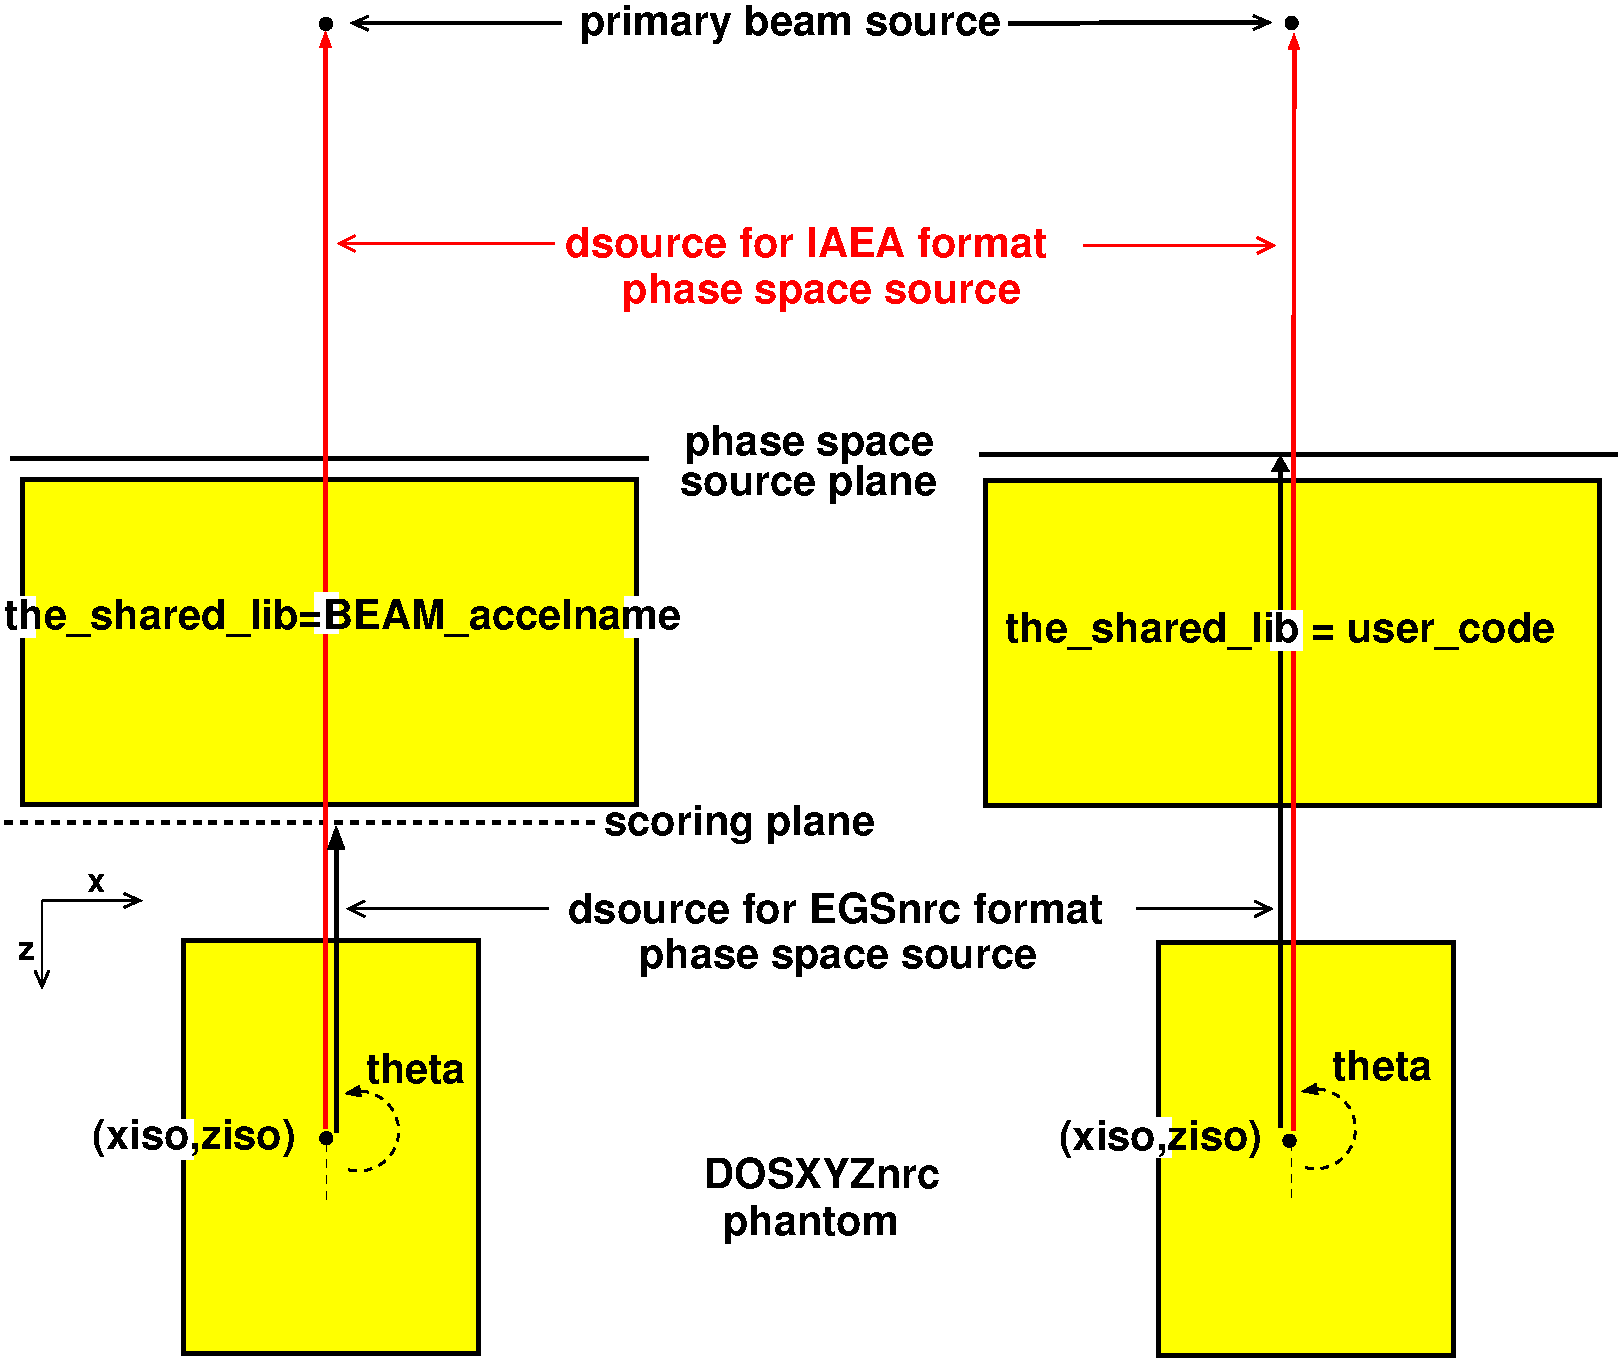
\includegraphics[width=17cm]{figures/src20_1}
\caption{Source 20 incident through a shared library (BEAM or non-EGSnrc user code).  When
the phase space source is run through a BEAM shared library geometry (left), {\tt dsource} defines
the distance between the centre of the scoring plane at the bottom of the geometry and the isocentre (BEAMnrc
phase space source, black arrow), or the distance between the primary source and the isocentre (IAEA phase
space source, red arrow).
When a non-EGSnrc code is used (right), {\tt dsource} defines the distance between the phase space source
and the isocentre (EGSnrc-format phase space source, black arrow) or between the primary source and the isocentre (IAEA phase space
source, red arrow).}
\label{fig_src20_1}
\end{center}
\end{figure}


If a BEAM shared library is used the following conditions apply:
\begin{itemize}
\item The BEAM input file, {\tt the\_input\_file} must define a scoring plane at the bottom of the geometry.  Particle data
at this plane are not actually output but are stored in an internal array for eventual DOSXYZnrc transport through the
phantom.
\item If the source specified in the BEAM input file is a phase space source, it must not make use of the same phase space file as DOSXYZnrc source 20.  This causes a file opening conflict in some versions of
Fortran and will cause the run to fail.  Note that when BEAM is used to define a geometry
for source 20, the BEAM source is not used, so a dummy source of any type can be specified in the BEAM input
file.
\item With a BEAMnrc-format phase space source, the incident Z-position (in the BEAM frame) of the phase space source is
the same as the incident Z-position of the source as defined in the BEAM input file, {\tt the\_input\_file}.  The source 20 input,
{\tt dsource} then defines the distance from the phantom isocentre to the centre of the scoring plane.
\item If an IAEA-format phase space source is used, the incident Z-position of the phase space source is read from
the phase space data itself.  Note that this means the user must ensure consistency between the geometry defined in
BEAM and the incident Z-position of the particles.  The input parameter, {\tt dsource}, defines the distance from
the isocentre to the primary beam source ({\tt i.e.} {\tt dsource}=SAD, see red arrow in figure)
\item The pegs data used in the accelerator simulation is not an input variable and must be the
same as that used in the DOSXYZnrc phantom.
\end{itemize}

If the phase space source is run through a non-EGSnrc shared library (compiled from {\tt user\_code})
the following applies:
\begin{itemize}
\item Phase space data below the defined geometry need not be scored.
\item If a BEAMnrc-format phase space source is used, the incident Z-position (in the {\tt user\_code} frame) is defined
as {\tt dsource}.  Thus, the user must ensure that the source plane is positioned correctly relative to the
defined geometry.
\item For an IAEA-format phase space source, the incident Z-position is read from the phase space source, and
{\tt dsource} defines the primary source-to-isocentre distance.  Again, the user must ensure consistency
between the incident Z-position and the dimensions of the geometry defined in {\tt user\_code}.
\end{itemize}

\indexm{source 20!NRCYCL}
\indexm{source 20!survival ratio}
One issue when running source 20 through a shared library is the determination of how many times
to recycle incident particles so that the phase space source does not rewind, causing loss of information
about particle correlations and subsequent underestimation of dose uncertainties.  As mentioned in Section~\ref{nrcycl}
below, DOSXYZnrc automatically estimates the number of times to recycle each particle, {\tt NRCYCL}, based on
the number of particles in the phase space source, the number of histories requested, and the charge of particles
requested.  However, interactions in the shared library geometry will change the number of particles reaching
the DOSXYZnrc phantom per particle incident from the phase space source.  Thus, the original estimate of
{\tt NRCYCL} is incorrect.  To overcome this when a BEAM shared library is used, an initial calibration comprising
1x10$^6$ particles run through the BEAM geometry only is used to determine the ratio of the number of particles
emerging from the bottom of the BEAM library geometry to the number of incident particles (survival ratio).
{\tt NRCYCL} is then recalculated by multiplying the original estimate by 1/(survival ratio).

\indexm{calflag}
Depending on the shared library geometry, the calibration run can consume
significant CPU time at the beginning of the simulation.  Therefore, if there is a sufficient number of particles in
the phase space source that the user is confident rewinding the source is not an issue, the calibration run can
be skipped by setting the input, {\tt calflag}, to 1.

If a
non-EGSnrc shared library
is used, then the user must provide a routine to estimate the survival ratio of particles passing through the
geometry.  This will be covered in more detail below.

\indexm{synchronized CMs}
When a BEAM shared library geometry includes synchronized component modules (CMs), such as SYNCJAWS, SYNCVMLC or SYNCMLCE,
then the opening coordinates of these component modules (defining the field) can be synchronized with the orientation of the phase space source
plane relative to the phantom.  In this case the value of {\tt MU\_RND}, used to set the incident source orientation (see above), is passed from
DOSXYZnrc to BEAM, where it is then used to set the opening coordinates of any synchronized CMs.
The user controls the synchronization between CM geometries and the incident source orientation using files (one for
each synchronized CM) that associate a field (set of opening coordinates) with a range of fractional monitor units.
See the BEAMnrc Users Manual\cite{Ro09} for more information
about synchronized CMs.

{\bf Non-EGSnrc Geometry Code ({\tt user\_code})}

\indexm{load\_vculib.c}
\index{particleDMLC}
The coding which allows a non-EGSnrc user code compiled as a shared library to communicate with
DOSXYZnrc is found in the C code, {\tt \$HEN\_HOUSE/cutils/load\_vculib.c}. The acronym ``vcu'' stands for
``Virginia Commonwealth University'' and is a reference to the fact that the Lobo and Popescu\cite{LP10}
used a simplified MLC geometry simulation developed at VCU, called {\tt particleDMLC}\cite{Si02}, as a shared
library geometry in simulations with source 20.

\indexm{non-EGSnrc shared library}
\indexm{non-EGSnrc shared library!system requirements}
System requirements for the use of a non-EGSnrc shared library with source 20 (or 21)
are the same as those for a
BEAM simulation source (see Section~\ref{src9sect} above).  Unix/Linux systems must have
a working C/C++ compiler so that {\tt load\_vculib.c} can be compiled to create the
object file, {\tt load\_vculib.o}.  If a working C/C++ compiler is detected on installation
of BEAMnrc/DOSXYZnrc then this is done automatically.  Windows systems do not require
a working C/C++ compiler, since a precompiled version of {\tt load\_vculib.o} is provided.
In addition, the file,
{\tt \$HEN\_HOUSE/specs/dosxyznrc\_config.spec}, where {\tt config} is the configuration
name, must have the
variable {\tt VCULIB\_OBJECTS} set to {\tt \$HEN\_HOUSE/lib/config/load\_vculib.o}
(note that a short form for this is {\tt \$EGS\_LIBDIR/load\_vculib.o})
prior to compiling DOSXYZnrc.  Again, this is set automatically on installation if
{\tt load\_vculib.o} was created successfully.

Currently, {\tt load\_vculib.c} is optimized for calls to subroutines defined in {\tt particleDMLC}. However,
the user can make changes to this file so that it is specific for calls to their own geometry code.  For illustrative
purposes, the following functions must be defined in the user's geometry code, assuming they have made
no changes to {\tt load\_vculib.c} or the DOSXYZnrc coding:

\begin{enumerate}
\indexm{initvcu}
\item{\bf \tt initvcu(char *the\_input\_file, float *survival\_ratio)}
An initialization routine which reads an input file for the geometry code ({\tt the\_input\_file}) and generates
an estimate of the survival ratio of particles between the phase space source and the bottom of the user code
geometry (usually a simulation of an MLC).  The input file would likely specify the geometry parameters and
would also pass the name of the phase space source to the user code.
The survival ratio is used to calculate the number of
times to recycle incident particles, {\tt NRCYCL} (see above).
\indexm{vculib\_sample}
\item{\bf \tt vculib\_sample(float *e, float *x, float *y, float *z, float *u, float *v, float *w, float *wt, int *iq,
 int *latch, int *nhist, int *more\_in\_container)}
A subroutine used to run the geometry code and sample particles reaching the bottom of the geometry.
The subroutine returns the phase space data for a particle at the bottom
of the geometry ({\tt e}=energy; {\tt x,y,z}=particle x,y,z-position; {\tt u,v,w}=x,y,z-direction cosines;
{\tt wt}=particle weight; {\tt iq}=charge; {\tt latch}=latch value), the number of primary histories
run to that point, {\tt nhist}, and an integer, {\tt more\_in\_container}, which is set to 0 if the storage
array for particles reaching the bottom of the geometry is empty ({\tt i.e.} the geometry simulation must
be run on the next call to {\tt vculib\_sample}).
\indexm{vculib\_finish}
\item{\bf \tt vculib\_finish()}
A subroutine called at the end of the simulation to close any files used by the geometry code, free up
reserved memory, etc.
\end{enumerate}

\indexm{source 20!IAEA phase space source}
\label{src20iaeasect}
\subsubsection{IAEA-format phase space sources}

Similar to other phase space sources (sources 2 and 8) source 20 is implemented such that if an IAEA-format phase space source is used, the
incident Z-position of
a particle is automatically read directly from the phase space data.  This eliminates the restriction imposed by BEAMnrc-format
phase space files of all particles being incident in the same plane and, thus, allows more flexibility
in terms of the phase space data that can be used.

\indexm{MU}
\indexm{MU\_RND}
If the IAEA phase space source includes the fractional monitor unit index, {\tt MU}, associated with each particle ({\it i.e.} 4-D data), then
a random value for {\tt MU}, {\tt MU\_RND}, is not chosen at the beginning of each history, and, instead, the value of
{\tt MU} read from the phase space data is automatically
used to set the incident source parameters (isocentre position, incident angle, etc) for the incident particle.
{\tt MU} is automatically
scored in IAEA phase space data output by BEAMnrc simulations using synchronized component modules (CMs) with time-varying opening coordinates
(see the BEAMnrc Users Manual\cite{Ro09}) and can also be included in IAEA phase space data output by DOSXYZnrc
simultions using synchronized sources (20 or 21) by using the {\tt i\_muidx\_out} input flag
(see description of input above and Section~\ref{phspoutsect}).  Thus, use of {\tt MU} read from
the phase space source allows synchronization of source 20 with upstream BEAMnrc simulations having synchronized
CMs or upstream DOSXYZnrc simulations with synchronized sources.

\indexm{spiral CT scan}
\subsubsection{Simulation of Spiral CT Scan}

A recent publication by Kim et al\cite{Ki13} details a modification of Source 8 (See Section~\ref{src8sect} above)
in which the phase space plane can be made to rotate in {\tt phi} about an isocentre which is concurrently
translating in Z, thus simulating exposure in a helical pattern.  Kim et al have used this to simulate dose due
to a spiral CT scan, and their results compare well with measurement.

Spiral scans can be modeled equally well using Source 20 (and 21, see below) using just two control points ({\tt nset}=2).
An example of two control points defining a spiral scan is:

\begin{verbatim}
0, 0, 0, 90, 0, 0, 15, 0
0, 0, 10, 90, 3600, 0, 15, 1.0
\end{verbatim}

These control points define simultaneous translation of the isocentre from {\tt z(1)}=0 to {\tt z(2)}=10 cm and rotation of the source plane
from {\tt phi(1)}=0 at {\tt z(1)} through {\tt phi(2)}=3600$^o$ at {\tt z(2)}.  The angular range, {\tt phi(2)}-{\tt phi(1)}, determines the
pitch of the helix.  In this example, the source rotates ten times (3600$^o$=10$\times$360$^o$) over a Z translation of 10 cm, so the pitch is
equal to 1.  The direction of rotation is determined by the sign of {\tt phi(2)}-{\tt phi(1)}.
If this is positive (as in this example), then rotation is clockwise about the Z-axis; if negative, rotation is counter-clockwise.  Note that the X- and Y-positions of the isocentre in this example remain unchanged, and {\tt theta} is fixed
at 90$^o$, which means the source-isocentre vector is perpendicular to the Z-axis.

The two control points in this example cover the entire range of fractional monitor units ({\it i.e.} {\tt muIndex(1)}=0, {\tt muIndex(2)}=1.0), and, thus,
include all incident particles.
However, using more control points to further subdivide the range, $[$0,1$]$, of fractional monitor units, it would be
possible to generate multiple spiral scans--having different pitch, Z-range, etc--in one simulation.

\subsection{isource = 21: Synchronized BEAM Simulation Source}
\label{src21sect}
\indexm{source routines!isource = 21}
\indexm{source routines!Synchronized BEAM Simulation Source}

Source 21 defines a BEAM treatment head simulation (compiled as a shared library) source incident over multiple ranges
of continuous motion with respect to angle, SSD and isocentre.  The source motion can be synchronized with the settings
of any synchronized component modules (CMs) in the accelerator.  There is also an option to run the source through
a geometry (usually MLC) defined by a non-EGSnrc user code, compiled as a shared library, placed between the treatment
head and the DOSXYZnrc phantom.  Source 21 was developed and contributed by Lobo and Popescu\cite{LP10}.  Just as
source 20 represents a significant enhancement over source 8 (phase space incident from multiple angles), source 21
represents a significant enhancement over source 10 (treatment head incident from multiple angles).

\indexm{source 21!system requirements}
The system requirements for running shared library sources are given in Section~\ref{src9sect} describing source 9 (BEAM
treatment head source incident from one direction).  Instructions on compiling a BEAM accelerator as a shared library
are also given there.

The input parameters for source 21 are:

\begin{description}
\item [~~~~{\tt iqin}]
\indexm{iqin}
Charge of the incident beam (-1: electron, 0: photon, 1: positron, 2: all particle types)
\item [~~~~{\tt isource}] = 21
\item [~~~~{\tt nset}]
\indexm{nset}
\indexm{\$MXANG}
The number of control points defining ranges of continuous source motion.  Same as for source 20 (see above).
{\tt nset} must be in the range 2 $\leq$ {\tt nset} $\leq$ {\tt \$MXANG}, where
{\tt \$MXANG} is defined in
the file {\tt \$EGS\_HOME/dosxyznrc/dosxyznrc\_user\_macros.mortran}.
\item [~~~~{\tt i\_dbs}]
\indexm{i\_dbs}
Set to 1 if directional bremsstrahlung splitting is used in the BEAM simulation and you wish
to reject photons directed outside the splitting field (which will all be fat). Set to 0 otherwise. Note that
{\tt i\_dbs} is read in as a real and converted to integer.
\item [~~~~{\tt e\_split}]
\indexm{e\_split}
Number of times to split charged particles as soon as they enter the phantom geometry. Split particles have their weight reduced by a factor of 1/{\tt e\_split}. This is only used in conjunction with photon splitting ({\tt n\_split}, see Section 8.16) to prevent higher-weight contaminant electrons from compromising statistics in photon beams. For maximum efficiency, it is suggested that you set {\tt e\_split=n\_split}, the photon splitting number.
\item [~~~~{\tt i\_muidx\_out}]
\indexm{i\_muidx\_out}
Set to 1 to include the fractional monitor unit index, {\tt MU}, associated with each particle in IAEA format phase
space output for particles leaving the phantom geometry.  Note that phase space data is not output at all
unless
\indexm{i\_phsp\_out}
{\tt i\_phsp\_out}, the input parameter in the main code controlling phase space output, is set to 1 or 2.
If {\tt MU} is included in the phase space output, then phase space data has a time dimension and is considered 4-D.
Scoring of {\tt MU} allows synchronization between the DOSXYZnrc simulation generating the file and any
downstream simulations--such as BEAMnrc simulations with synchronized component modules--using the file as
a source. See Section~\ref{phspoutsect} for a description of DOSXYZnrc phase space output.
\end{description}

For control points i=1,2,...,{\tt nset}, the following parameters defining the source orientation are entered:
\begin{description}
\item[~~~~{\tt xiso(i)/yiso(i)/ziso(i)}]
\indexm{xiso,yiso,ziso}
x-, y-, z-coordinates of the phantom isocenter.
\item[~~~~{\tt theta(i)}]
\indexm{theta(i)}
Angle of normal connecting origin of the BEAM scoring plane to the isocentre.
\item[~~~~{\tt phi(i)}]
\indexm{phi(i)}
Angle of normal connecting the origin of the BEAM scoring plane to isocentre relative to the +X axis.
\item[~~~~{\tt phicol(i)}]
\indexm{phicol(i)}
2D Angle of rotation of the BEAM scoring plane about its own origin.
\item[~~~~{\tt dsource(i)}]
\indexm{dsource(i)}
The length of the normal from the origin of the BEAM scoring plane to the isocentre.
\item[~~~~{\tt muIndex(i)}]
\indexm{muIndex(i)}
A monitor unit index in the range $[$0,1$]$ defining the fraction of the total number of incident primary histories
delivered up to control point i.  This is slightly different from source 20, where {\tt muIndex(i)} defines the fraction
of incident particles up to control point i.  Thus, for source 21, {\tt muIndex(i)} is actually related to the fractional
monitor units delivered by the BEAM simulation.
Note that {\tt muIndex(i)} $\geq$ {\tt muIndex(i-1)}. Also note that for correct selection of the range
of incident source parameters, {\tt muIndex(1)=0.0} and {\tt muIndex(nset)=1.0}.
\end{description}
This is the end of inputs required for each control point.

\begin{description}
\item[~~~~{\tt the\_beam\_code}]
\indexm{the\_beam\_code}
The name of the BEAM accelerator code ({\it i.e.} {\tt BEAM\_accelname}) used to run the treatment head
simulation.  This must have been compiled as shared library ({\it e.g.} {\tt libBEAM\_accelname.so} on a Linux/Unix system) existing
in your {\tt \$EGS\_HOME/bin/config} directory.
\item[~~~~{\tt the\_input\_file}]
\indexm{the\_input\_file}
The input file for the BEAM treatment head simulation.  This must exist in directory {\tt \$EGS\_HOME/BEAM\_accelname} and must
specify a single scoring plane (usually at the bottom of the accelerator).
\item[~~~~{\tt the\_pegs\_file}]
\indexm{the\_pegs\_file}
The PEGS data to be used in the BEAM treatment head simulation.
\indexm{the\_vcu\_code}
\item[~~~~{\tt the\_vcu\_code}]
This optional input is the name of a non-EGSnrc user code, compiled as a shared library, that can be used to define a geometry
through which particles are run between the bottom of the treatment head and the DOSXYZnrc phantom.  The shared library must
exist in directory {\tt \$EGS\_HOME/bin/config}
\indexm{the\_vcu\_input\_file}
\item[~~~~{\tt the\_vcu\_input\_file}]
Input file for {\tt the\_vcu\_code} defining the geometry interposed between the treatment head simulation and the phantom.
\end{description}

\indexm{\tt MU\_RND}
For each primary history in the treatment head simulation a random fractional monitor unit index, {\tt MU\_RND}$\in[$0,1$]$, is
chosen.  {\tt MU\_RND} is either generated by DOSXZYnrc or, if there are synchronized CMs in the treatment head simulation also
undergoing motion, it is passed to DOSXYZnrc from the BEAM simulation.  More details on the use of synchronized CMs in the BEAM
simulation are given below.  For all particles associated with a given value of {\tt MU\_RND}, the control points, i-1 and i,
within which the source position falls are those for which {\tt muIndex(i-1)}$\leq${\tt MU\_RND}$<${\tt muIndex(i)}, and the
parameters determining the source orientation are calculated using Equation (1) (see Section~\ref{src20sect} above).
Note that, unlike source 20, {\tt MU\_RND} is chosen only for each primary history, not for each incident particle.  Thus,
the {\tt muIndex(i)} for the control points are traceable to actual monitor units in the treatment head.

Recall that the source plane is actually the phase space scoring plane in the BEAM treatment head, defined in {\tt the\_input\_file}.
Phase space data is not output at this plane but is stored in an internal array for use by DOSXYZnrc over the course of the
simulation.

\indexm{i\_dbs}
Similar to source 9 (See section~\ref{src9sect}), since the BEAM simulation is running
concurrently with DOSXYZnrc, if directional bremsstrahlung splitting (DBS) is being used
in BEAM, information about whether or not a particle has been split or has survived
russian roulette (``fat'' particles) is available without having to reconstruct the DBS splitting
field after the fact.  Thus, fat photons can be rejected from the DOSXYZnrc simulation simply
by setting {\tt i\_dbs}=1 and the additional inputs required to reject fat photons from
phase space sources,  {\tt r\_dbs}, {\tt ssd\_dbs}, {\tt z\_dbs} (See Section~\ref{src20sect})
are not required.

\indexm{enflag}\indexm{mode}\indexm{zlast}
As with other phase space and BEAM simulation sources, the input {\tt enflag} must be set
to 2 or 3 to indicate whether {\tt LATCH} bit filtering is to be used, the mode of the
data (with or without {\tt zlast}) being read from the BEAM simulation must be indicated, and
the medium and thickness of the medium surrounding the phantom ({\tt dsurround}) must be
input.  For more information on these inputs, see Section~\ref{sec5}.

\indexm{source 21!use of synchronized CMs}
\subsubsection{Use of synchronized CMs in the BEAM simulation}

If the BEAM treatment head simulation includes synchronized component modules, such as SYNCJAWS, SYNCVMLC, and SYNCMLCE, and
the user is modeling dynamically-changing field coordinates with them, then {\tt MU\_RND} for each primary history is passed
from BEAM to DOSXYZnrc, and the user can synchronize the orientation of the source plane with the field coordinates through
the {\tt muIndex(i)} of the individual control points.  Synchronized CMs are also synchronized with each other.  For more information
on the synchronized CMs, see the BEAMnrc Users Manual\cite{Ro09}.

Figure~\ref{src21_fig} below shows visually how the incident source orientation may be synchronized with the CM settings.

\begin{figure}[htbp]
\begin{center}
\hspace*{-1cm}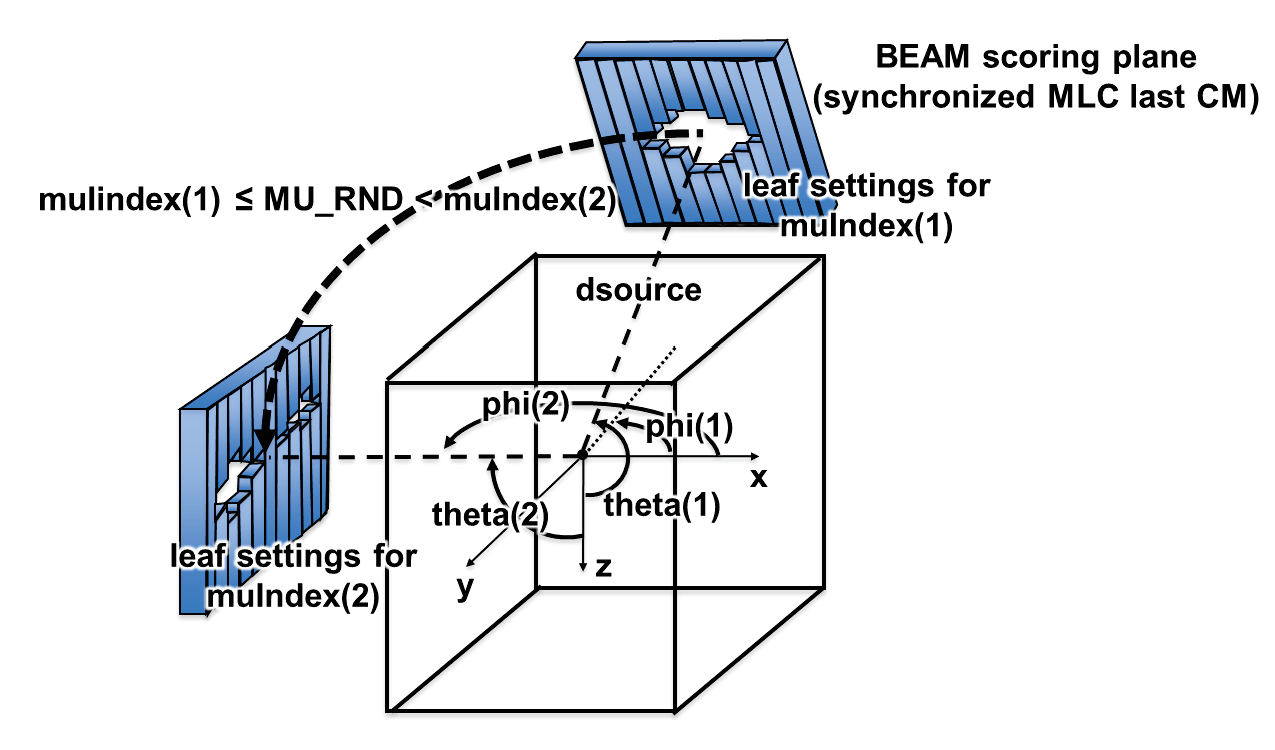
\includegraphics[width=18cm]{figures/src21_fig}
\caption{Source 21, including a synchronized CM, incident on a DOSXYZnrc phantom.  The figure indicates that the final CM in the treatment head
simulation is a synchronized MLC (SYNCVMLC, SYNCMLCE or SYNCHDMLC).  Two control points for the source plane, having different
{\tt muIndex}, {\tt theta} and {\tt phi}, are
indicated.  Different MLC leaf settings are also associated with the values of {\tt muIndex} (the user sets this up in
a file read by the synchronized CM).  Continuous motion of the source between ({\tt theta(1), phi(1)}) and ({\tt theta(2), phi(2)}), along
with dynamic motion of the MLC leaves,
is simulated for values of {\tt MU\_RND} with {\tt muIndex(1)}$\leq${\tt MU\_RND}$<${\tt muIndex(2)}.  Continous motion in
{\tt dource}, isocentre position ({\tt xiso, yiso, ziso}), and the angle of rotation of the source plane in the plane ({\tt phicol}) can
also be simulated.}
\label{src21_fig}
\end{center}
\end{figure}

\indexm{source 21!and non-EGSnrc shared library}
\subsubsection{Running the source through a non-EGSnrc shared library}

\indexm{the\_vcu\_code}\indexm{the\_vcu\_input\_file}
Using the inputs {\tt the\_vcu\_code} and {\tt the\_vcu\_input\_file} the user has the option to interpose another geometry
(usually an MLC) between the source plane and the DOSXYZnrc phantom.  In general, {\tt the\_vcu\_code} is a non-EGSnrc user
code.  Lobo and Popescu\cite{LP10} have used a version of the code particleDMLC\cite{Si02}, developed at Virginia Commonwealth University (hence ``vcu'' in the variable names), to place a simplified MLC simulation between the source and the phantom.

A detailed discussion of potential user codes for creating simplified MLCs is beyond the scope of this manual.  However,
a summary of the subroutines that must exist in {\tt the\_vcu\_code} and the parameters required to communicate
with DOSXYZnrc is given in the description of source 20 (Section~\ref{src20sect}) above.

Note that with source 21, {\tt dsource} always defines the Z-position, in the BEAM frame, of the source plane (scoring plane in the BEAM simulation), and
it is up to the user to ensure that the source is positioned correctly relative to the geometry
defined by {\tt the\_vcu\_code}.


\rfoot[{\sffamily \rightmark}]{{\sffamily \leftmark}}

\section{Other Source-Related Inputs}
\label{sec5}
After the inputs described above, there is another record input with
several other variables related mostly to the source.

\indexm{enflag}
\subsection {{\tt enflag}}
\label{enflag_sect}
The setting of {\tt enflag} determines whether the source is monoenergetic
or has an energy spectrum, or, if the source is a phase space file, whether
or not a dose component is to be calculated.
The possible settings of {\tt enflag} are:
\begin{description}
\item [~~~~= 0] (default) for a monoenergetic source ({\tt isource}=0,1,3,6).
\item [~~~~= 1] for an energy spectrum input ({\tt isource}=0,1,3,6).
\item [~~~~= 2] for a phase space source ({\tt isource}=2) or
full BEAM simulation source ({\tt isource}=9), no dose component
calculation.
\item [~~~~= 3] for a phase space source ({\tt isource}=2) or
full BEAM simulation source ({\tt isource}=9), dose component
calculation using a bit filter (see section~\ref{bitfiltersec} below).
\item [~~~~= 4] for a beam characterization model source ({\tt isource}=4).
\end{description}

\subsection {{\tt mode}}
\indexm{mode}
{\tt mode} only has meaning for a phase space source ({\tt isource}=2).
However, an explicit value for {\tt mode} must exist in the input file
for a full BEAM simulation source ({\tt isource}=9) or
beam characterization model source ({\tt isource}=4), since
{\tt isource}=4 and 9 make use of {\tt medsur}, {\tt dflag} and {\tt dsurround},
which occur after {\tt mode} on the same line.
The possible settings of {\tt mode} are:
\begin{description}
\item [~~~~= 0] (default) the phase space source does not contain
{\tt ZLAST} (for photons, Z of last site of interaction; for electrons,
Z where electron or its ancestor was set in motion by a photon) and, thus,
has 7 variables/record.
\item [~~~~= 2] the phase space source contains {\tt ZLAST} and, thus,
has 8 variables/record.
\end{description}

Note that DOSXYZnrc does not make use of {\tt ZLAST}, but it needs to know
whether {\tt ZLAST} is in the file or not so that the appropriate number
of variables/record can be read.  Thus, if a phase space file is only
going to be used as a source for a DOSXYZnrc calculation, you can save space
by leaving {\tt ZLAST} out of the file.  For more information
about {\tt ZLAST}, see the BEAMnrc Users Manual\cite{Ro09}.

\subsection {{\tt medsur}}
\indexm{medsur}
{\tt medsur} is the medium number for the region surrounding the phantom
as defined by {\tt dsurround}
(see below).  {\tt medsur} is only input for phase space, full BEAM
simulation or beam characterization
model sources ({\tt isource}=2, 4, 8 or 9).  The default setting of {\tt medsur}
is 0, indicating the
surrounding region is vacuum.  However, the user may set this to correspond
to any of the media that they have defined at the top of the DOSXYZnrc input file.
In many cases, the user may wish to fill this region with air and have particles
transported properly through air before reaching the phantom.

\subsection{{\tt dsurround} and {\tt dflag}}
\label{dflagsect}
\indexm{dsurround}
\indexm{dflag}

{\tt dsurround} and {\tt dflag} are required for phase space, full
BEAM simulation and
beam characterization model sources {\tt isource}=2, 4, 8, 9, 10, 20 or 21.
These inputs define the dimensions of the region surrounding the phantom
(ie filled with the medium defined by {\tt medsur}).  Note that
{\tt dsurround} is a 4-dimensional array
with {\tt dsurround(1)} occurring before {\tt dflag} on the input line
and {\tt dsurround(2...4)}, if required, occurring after {\tt dflag}.

The possible settings for {\tt dflag} and their relation to {\tt dsurround}
are as follows:

\begin{description}

\item [~~~~{\tt dflag}=0] (default) {\tt dsurround(1)} defines the thickness
if the surrounding region (in cm) on all sides of the phantom, and the user
need not
input values for {\tt dsurround(2...4)}.  {\tt dsurround(1)}
defaults to 50 cm if it is set $\leq$0.
\item [~~~~{\tt dflag}=1] means that {\tt dsurround(1)} defines the thickness of the
surrounding region in the $\pm$x directions, {\tt dsurround(2)} is the
thickness of the surrounding region in the $\pm$y directions, {\tt dsurround(3)}
is the thickness in the +z direction (bottom of the phantom)
and {\tt dsurround(4)} is the thickness
in the $-$z direction (top of the phantom).  {\tt dsurround(1...4)} default to 0.
\end{description}

Use of {\tt dflag}=1 with {\tt dsurround(1...4)} can save substantial amounts of
computing time if the user is only interested in the dose along a certain axis
or in a specific slice of a DOSXYZnrc phantom (see section~\ref{dsurround_section}
below).

\subsection{{\tt ein}}
\indexm{ein}

{\tt ein} is the kinetic energy of
a monoenergetic incident beam in MeV.  It defaults to 1.25 MeV if
{\tt ein} is set $\leq$ 0.  Note that {\tt ein} is only required if
{\tt isource}=0,1,3,6 and {\tt enflag}=0.

\subsection{{\tt FILNAM}}
\indexm{FILNAM}

{\tt FILNAM} is the file name (with extension) of:

\begin{description}
\item[incident beam energy spectrum] if {\tt isource}=0,1,3 or 6 and
{\tt enflag}=1.  In this case, {\tt FILNAM} has a specific format which
corresponds to the ensrc format used in the original EGSnrc system
\indexm{energy spectrum format}
(see {\tt \$HEN\_HOUSE/spectra} for a large number of
example spectra):

{\tt ENSRC.V5 File format\\
====================}
\begin{tabbing}
\= {\tt SPEC\_TITLE} \\
\> {\tt NENSRC, ENMIN, IMODE} \\
\> {\tt ENSRCD(I), SRCPDF(I) (I = 1 to NENSRC)} \\
\end{tabbing}
\vspace*{-5mm}
where:
\vspace*{-3mm}
\begin{description}
\item [~~~~{\tt SPEC\_TITLE}] is an 80-character spectrum title
\item [~~~~{\tt NENSRC}] = \# of energy bins in the spectrum histogram
\item [~~~~{\tt ENMIN}] = lower energy of first bin in MeV
\item [~~~~{\tt IMODE}] Set to 0 for histogram counts/bin; set to 1 for
counts/MeV
\item [~~~~{\tt ENSRCD(I)}] = upper energy of bin I in MeV
\item [~~~~{\tt SRCPDF(I)}] = probability of finding a particle in bin
I (SRCPDF
need not be normalized)
\end{description}

\item[phase space source:] if {\tt isource}=2 or 8 and {\tt enflag}=2 or 3.
See Section~\ref{source2sect} for more details.
\item[beam characterization model:] if {\tt isource}=4 and {\tt enflag}=4.
\indexm{the\_beam\_code}
\indexm{the\_input\_file}
\indexm{the\_pegs\_file}
\item[{\tt the\_beam\_code}, {\tt the\_input\_file}, {\tt the\_pegs\_file}:]
if {\tt isource}=9 or 10 and {\tt enflag}=2 or 3.  These are the names of the
BEAM accelerator code being used as a source, the input file for the BEAM
simulation, and the pegs data for the BEAM simulation respectively.  See
section~\ref{src9sect} for more details.
\end{description}

\subsection{{\tt IOUTSP}}
\indexm{IOUTSP}
{\tt IOUTSP} is only required with an incident energy spectrum ({\tt enflag}=1).  The
possible settings of {\tt IOUTSP} are:

\begin{description}
\item [~~~~= 0] (default) no output summary of incident energy spectrum
in {\tt .egslst}.
\item [~~~~= 1] output a summary of the incident energy spectrum to the
{\tt .egslst} file.
\end{description}

\section{Phase Space Sources}
\index{phase space sources}

The phase-space files output by BEAMnrc and used by DOSXYZnrc for sources 2 and 8 are
described in detail in section 7 of the BEAMnrc User's Manual.
\cite{Ro04a}.

The phase-space files are binary files  opened with ACCESS = 'direct' and
FORM = 'unformatted'.  Because they are binary files, and because there
are two common byte orders used for binary files by different systems
(eg PCs and DEC machines use one form and SUNs and SGIs use the other),
files written by one system may not be compatible with another system.
The utility {\tt readphsp} found on {\tt \$OMEGA\_HOME/progs/readphsp} can
convert files from one format to the other (see the description in the BEAMnrc
User's Manual. \cite{Ro04a}.)

There are also two types of phase-space files determined by how many
variables they contain.  The shorter format is
called '{\tt MODE0}' and  {\tt ZLAST} is not
scored and the longer format is
'{\tt MODE2}' when {\tt ZLAST} is present.  Since DOSXYZnrc makes no use of
the {\tt ZLAST} variable, it saves space to use {\tt MODE0} files for use with
DOSXYZnrc.  The '{\tt MODE0}' or '{\tt MODE2}'
designation appears in the first record of a phase-space file along
with the total number of particles contained in the file, the number
of photons, maximum energy of any particle in the file,
minimum energy of electrons, and minimum energy of
photons.

\indexm{phase space sources!negative energy marker}
\indexm{phase space sources!using old files}
\indexm{uncertainties}
\indexm{statistics}
Phase space files generated by BEAMnrc use negative
{\tt E} (energy) to mark the first particle scored by each new primary
history.  If the file is used as a source, then the negative {\tt E} marker
allows scored quantities (ie energy deposited) to be grouped according
to primary history.  This ensures that uncertainties estimated account
for the correlations between incident particles in a phase space
source~\cite{Wa02a}.  If an old phase space file without negative {\tt E} markers is used
as a source, then scored quantities will be grouped according to incident
particle instead of primary history.  DOSXYZnrc will then output a warning
that uncertainty may be underestimated because correlations between incident
particles could not be taken into account.  This is not a cause for concern,
because we have found~\cite{Wa02a} that in the cases we studied,
the underestimate is not significant.

When using a phase space source, if the entire phase space file is read
before the requested number of histories is run, then DOSXYZnrc restarts
the phase space file from the beginning.  For the reasons discussed in
section~\ref{nrcycl}, page~\pageref{nrcycl}, this is not a desirable
occurrence and one should strive to avoid this by using the recycling
feature (which also saves on reading time).

\index{IAEA-format phase space sources}
\label{iaeaphspsect}
\subsection{IAEA-format Phase Space Sources}

In addition to the standard BEAMnrc phase space files described
above, DOSXYZnrc can
also use IAEA-format phase space data as a source.  This allows the
user to make use of IAEA's online data base of accelerator phase space
data at:\\
\htmladdnormallink{www-nds.iaea.org/phsp/phsp.htmlx}{http://www-nds.iaea.org/phsp/phsp.htmlx}

\index{C++ compiler}
Note that this functionality requires that EGSnrc/DOSXYZnrc be installed on a machine
with a working C++ compiler.  This is detected automatically during
EGSnrc installation and, if a working C++ compiler is found, the library
of IAEA phase space handling routines is compiled.

\index{{\tt .IAEAheader}}
\index{{\tt .IAEAphsp}}
\index{IAEA phase space data! header file}
\index{IAEA phase space data! phase space data file}
Phase space data in IAEA format comprises both a header
(extension {\tt .IAEAheader}) file and a phase space data
(extension {\tt .IAEAphsp}) file.  When using IAEA phase space data as
a source, only the full name and directory path of the {\tt .IAEAphsp} file needs to be specified
(See Section~\ref{source2sect}).  The {\tt .IAEAheader} file is assumed to be
in the same directory.

Note that when IAEA phase space sources are used the incident Z-position of each particle
is available and is automatically read, either from the header file in the case of
planar phase space data (such as that scored by BEAMnrc), or from the phase space
data itself if it is scored in 3-D (such as that scored by DOSXYZnrc).  The ability to handle
3-D phase space data greatly enhances the flexibility of DOSXYZnrc and allows it to
use non-planar data supplied by manufacturers, such as that supplied by Varian for
their TrueBeam accelerators.  In addition, IAEA phase space files generated by BEAMnrc simulations
with synchronized component modules (CMs) and by DOSXYZnrc simulations using synchronized
sources (20 or 21) may include the fractional monitor unit ({\tt MU}) associated with each particle.
This is automatically read in and used by DOSXYZnrc's synchronized phase space source (source 20) allowing
synchronization between the DOSXYZnrc simulation and the upstream simulation that generated the phase
space file.  See Sections~\ref{src2iaeasect} and \ref{src20iaeasect} for more information.

Form more information on the format of IAEA phase space data, see the
BEAMnrc Manual and IAEA Report INDC(NDS)-0484\cite{CJ05}.

\section{Calculating Dose Components with DOSXYZnrc}
\label{bitfiltersec}
\subsection{Bit Settings}
\indexm{bit setting}

\indexm{LATCH}
The {\tt LATCH} variable, associated with each particle in a
BEAMnrc simulation, is a
32-bit variable used to track the particle's history.  It is discussed in
detail in the BEAMnrc User's Manual \cite{Ro04a}.

Each bit in {\tt LATCH} is designated as follows with bit 0 being the lowest value bit:
\begin{description}
\item [~~~~bit 0] Set to 1 if a photon is created by a bremsstrahlung event or an electron is created by a bremsstrahlung photon; 0
otherwise
\item [~~~~bits 1-23] Used to record the region where a particle has been and/or
has interacted. Note that the bit set for a region is determined by
{\tt IREGION\_TO\_BIT} (which is defined in the BEAMnrc simulation)
for that region.
\item [~~~~bits 24-28] Stores {\tt IREGION\_TO\_BIT} (as a binary number) of the
region in which a secondary particle
is created; if these bits are all 0, the particle is a primary
particle
\item [~~~~bits 29-30] Store the charge of a particle at the time {\tt LATCH} is output
\indexm{LATCH}
to a phase-space file.
\item [~~~~bit 31] Set to 1 if a particle has crossed a scoring plane
more than once when {\tt LATCH} is output to a phase-space file.
\indexm{LATCH}

\end{description}

For secondary particles, recording the {\tt IREGION\_TO\_BIT}'s of
the regions in which they were
created in bits 24-28 is equivalent to multiplying the {\tt IREGION\_TO\_BIT} by
2$^{24}$, or 16777216.  Thus, to retrieve {\tt IREGION\_TO\_BIT} of the region
of origin of a
secondary particle, the {\tt LATCH} value of the particle must be divided by
16777216 (i.e., taking the value {\tt INT(LATCH/16777216)}).
\indexm{LATCH}

When used with a phase space source, DOSXYZnrc has the
capability of selecting from the phase space file only those particles that
have user-specified bits (called a ``bit filter") set in their {\tt LATCH}
variables.
Thus, DOSXYZnrc will score only the dose component arising from these user-selected
particles.  For example, in the BEAMnrc simulation, bit 10 may be associated
with a square applicator, so any particle in the phase space file that has
been in the applicator will have bit 10 set in {\tt LATCH}.  When using
this phase space file as a source in DOSXYZnrc, the user may opt to use only
those particles that have bit 10 set, thus scoring the dose component from
particles that have been in the applicator.

In general, a dose component can be selected
according to what regions particles have passed through/interacted in,
whether the particle is a primary or secondary, if the particle is a
secondary then where it was created, and any combination of these.

\subsection{Input for Dose Component Calculations}

In order to enable dose component calculations with a phase space source
or full BEAM simulation source
({\tt isource}=2, 8 or 9),
the variable {\tt enflag} must be set to 3.  The user then specifies which
\indexm{enflag}
type of bit filter ({\tt I\_BIT\_FILTER}) to use.  Below is a description of the
4 types of bit filters available and the inputs associated with each.

\begin{description}
\indexm{I\_BIT\_FILTER}
\indexm{NBIT1}
\indexm{NBIT2}
\indexm{BIT}
\index{IREGION\_TO\_BIT}
\item [{\tt I\_BIT\_FILTER}=0] This is an inclusive/exclusive bit filter.  On the
same line as {\tt I\_BIT\_FILTER}, the user inputs the integers {\tt NBIT1} and
{\tt NBIT2}.  {\tt NBIT1} is the number of bits to include and {\tt NBIT2} is
the number of bits to exclude.  Restriction is that
0$\leq${\tt NBIT1}+{\tt NBIT2}$\leq$29.
Both {\tt NBIT1} and {\tt NBIT2} can be set to zero.  On the next line, the
user inputs {\tt BIT(I) (I=1,NBIT1)}, the bits to be included, and on
the following line \\ {\tt BIT(I) (I=NBIT1+1,NBIT1+NBIT2)}, the bits to
be excluded.  If any of the first set of {\tt NBIT1} bits are set and none
of the second set of {\tt NBIT2} bits are set in the particle's {\tt LATCH}
variable, the particle is used in the
simulation.

\item [{\tt I\_BIT\_FILTER}=1] This is an exclusive bit filter.  On the same line
as {\tt I\_BIT\_FILTER}, the user inputs the integer {\tt NBIT1}, the
number of bits to be excluded (0$\leq${\tt NBIT1}$\leq$29).  {\tt NBIT2} is
not relevant for this filter and is automatically set to 0.  On the
next line, the user inputs, {\tt BIT(I) (I=1,NBIT1)}, the bits to
be excluded.  If any of these {\tt NBIT1} bits are set in the particle's
{\tt LATCH} variable, the particle
is NOT used in the simulation.

\item [{\tt I\_BIT\_FILTER}=2] An inclusive region-of-origin filter.
The user inputs {\tt NBIT1} on the same line
as {\tt I\_BIT\_FILTER}, where {\tt NBIT1} is the number of regions of origin
to be included.  Since regions of origin are distinguished only by their
values of {\tt IREGION\_TO\_BIT}, {\tt NBIT1} can also be seen as the
number of distinct values of {\tt IREGION\_TO\_BIT} to be included. The
restriction on {\tt NBIT1} is 0$\leq${\tt NBIT1}$\leq$24.  {\tt NBIT2} is
not relevant for this filter and is automatically set to 0.  On the
next line, the user inputs {\tt IREGION\_TO\_BIT(I) (I=1,NBIT1)}, the
{\tt IREGION\_TO\_BIT} values of the {\tt NBIT1} regions of origin to
be included.  If the particle originated in any one of these {\tt NBIT1}
regions, then it will be used in the simulation.  Primary particles will be included if
{\tt IREGION\_TO\_BIT=0} is one of the {\tt NBIT1} values of
{\tt IREGION\_TO\_BIT} to include.

\item [{\tt I\_BIT\_FILTER}=3] An exclusive region-of-origin filter.
The user inputs {\tt NBIT1} (0$\leq${\tt NBIT1}$\leq$24), the number of
regions of origin to be excluded, on the same line as {\tt I\_BIT\_FILTER} and
ignores {\tt NBIT2}, since it is not relevant for this filter.  On the
next line the user inputs {\tt IREGION\_TO\_BIT(I) (I=1,NBIT1)}, the
{\tt IREGION\_TO\_BIT} values of the regions of origin to be excluded.
If a particle originated in any one of these regions, then it is NOT
used in the simulation.  Note that primary particles will be excluded if
{\tt IREGION\_TO\_BIT=0} is one of the {\tt NBIT1} values of
{\tt IREGION\_TO\_BIT} to exclude.

\end{description}

Note that since only one bit filter can be input per simulation, only one
dose component may be calculated at a time using DOSXYZnrc.  This is because
of the large memory requirements for the dose scoring arrays.

\section{Other Input Variables}

This section provides descriptions of main DOSXYZnrc input variables not
covered above.

\vspace*{-0.5cm}
\subsection{{\tt IPHANT}}
\label{iphantsect}
\indexm{IPHANT}

If {\tt IPHANT} is set to 1, DOSXYZnrc outputs phantom data to
a {\tt .egsphant} file.  This file has the same format as the
{\tt .egsphant} file that {\tt ctcreate} outputs for CT data
(see section~\ref{egsphantsect}) and can be read by
{\tt dosxyz\_show}\cite{Ka98},
along with the {\tt .3ddose} dose output file to display isodose contours in
the phantom.  Note that this option is redundant (and, therefore, unavailable)
when using a CT phantom because it is an input file from ctcreate).

\subsection{{\tt MAX20}}
\indexm{MAX20}
\label{MAX20description}

When {\tt MAX20} is set to 1, a summary of the maximum 20 doses in the
phantom is output to the screen (log file) and list file.  This summary
includes an output of the 20 maximum doses with their fractional
uncertainties and coordinates, the average of the 20 maximum doses, the average
fractional uncertainty of these doses (not the uncertainty of the average), the
average fractional uncertainties of all doses $>$ 50\% of the maximum dose,
and the average absolute uncertainty of all doses $>$ 50\% of the maximum dose
as a fraction of the maximum dose.

When not in CT phantom mode, {\tt MAX20} is the last variable on the line(s)
specifying the regions for which dose will be output (ie record 9).  If
{\tt MAX20} is set to 1 on ANY ONE of these lines (including the line of
zeros indicating the end of this record) then the summary of the 20 maximum
doses will be output.

In CT phantom mode, {\tt MAX20} is input
\indexm{MAX20} on the same line as {\tt zeroairdose} and {\tt doseprint}.

This option is useful for timing/efficiency studies.
\subsection{{\tt zeroairdose}}
\indexm{zeroairdose}
\label{zeroairdose}

{\tt zeroairdose} is only used in CT phantom mode.
Setting {\tt zeroairdose} to 1 will set all dose estimates in
voxels with density $<$ 0.044 g/cm$^3$ to zero in the {\tt .3ddose}
\indexm{.3ddose}
\indexm{files!.3ddose}
file.  This has the effect of zeroing dose in voxels filled with air
(see the default CT ramp in Figure~\ref{fig_ct02}--note that ``AIR''
has a density ranging from 0.001-0.044 g/cm$^3$).
Air dose will not be zeroed in the {\tt .egslst} file, this file will
continue to report the precise estimated dose.  {\tt zeroairdose} serves
as a dose visualisation parameter for CT phantom simulations, since, in general, the user is only interested
in seeing the dose within the patient, not in the surrounding air.

\subsection{{\tt doseprint}}
\indexm{doseprint}

This input parameter is also only used in CT phantom mode.

{\tt doseprint} is set to 1 if the user wants a full output of doses in
all voxels of the CT phantom in the {\tt .egslst} file.  Since, in CT
phantom cases, the user is usually not interested in this output and, owing
to the large number of voxels in a CT phantom, it can make the {\tt .egslst}
exceptionally large, the default is to suppress this output (ie set
{\tt doseprint} to 0).

\subsection{{\tt NCASE}}
\indexm{NCASE}

{\tt NCASE} is the number of histories to run in a simulation.  Minimum
value is 100.  Default is 100 if {\tt NCASE} is set $<$ 100.  The number
of histories per output batch is equal to {\tt NCASE}/({\tt \$NBATCH}),
where {\tt \$NBATCH} is currently set to 10.

\subsection{{\tt IWATCH}}
\indexm{IWATCH}

{\tt IWATCH} controls output to the screen (interactive run) or to the
{\tt .egslog} file (batch run) during beam execution.  The possible settings
are:
\begin{description}
\item [~~~~= 0] (default) On completion of each batch, outputs information about the
batch (eg elapsed time, CPU time, elapsed/CPU time, random number used
to begin batch, \# of random seeds used in the batch, total number of
histories run up to and including the current batch, the total number of
particles scored in the first phase-space file)

\item [~~~~= 1] Outputs same information as 0 plus, after every particle
interaction, outputs complete information about the particle(s)
involved (eg interaction type, particle type, position of particle on
stack, particle energy, X-Y-Z position of particle, U-V-W direction
cosines, {\tt LATCH} value of particle, region \# of particle); also informs
\indexm{LATCH}
user when a particle is being discarded, when a particle is passing from
one CM to another

\item [~~~~= 2] Similar to 1 but with complete particle information output at
every step; also outputs total dose in a region whenever energy is
deposited there

\item [~~~~= 3] Similar to 2 but with particle and dose information output
whenever dose is deposited.

\item [~~~~= 4] Outputs same information as 0 plus {\tt .egsgph} and {\tt
.egsgeom} files for graphical representation of the accelerator and
particle paths using {\tt EGS\_Windows.}
\indexm{.egsgph}
\indexm{.egsgeom}
\indexm{files!.egsgph}
\indexm{files!.egsgeom}
\end{description}

\subsection{{\tt TIMMAX}}
\indexm{TIMMAX}

{\tt TIMMAX} is the maximum CPU time in hours allowed for a simulation.
{\tt TIMMAX} defaults to 0.99 hrs if it is set = 0.  However, this time-restriction function is not activated in the current version of DOSXYZnrc except to
print a warning as it starts a batch which will exceed this limit.


\subsection{{\tt INSEED1, INSEED2}}
\indexm{INSEED}
\indexm{RANMAR}
\indexm{RANLUX}
\indexm{random number generator}
\indexm{random number seeds/pointers}

These are random number seeds used to initialize the
RANMAR\cite{MZ91,Ma90a} or RANLUX\cite{La94,Ja94}
random number generator.  Within DOSXYZnrc,
{\tt INSEED1} is limited
to the range\\ 0$<${\tt INSEED1}$\leq$31328
(defaults to 1802), and {\tt INSEED2} has
the range 0$<${\tt INSEED2}$\leq$30081 (defaults to 9373).  These
ranges/defaults are designed for RANMAR (the default random number generator),
however, if
you are using RANLUX then {\tt INSEED1} is the ``luxury level"
of the random number generator and must be in the range
0$<${\tt INSEED1}$\leq$4, otherwise, it will automatically be set to the
default luxury level of 1 (Note: this means that the DOSXYZnrc default value
for {\tt INSEED1} of 1802 will ultimately get reset to 1 by RANLUX).

Note that \verb+INSEED1+ and \verb+INSEED2+ are only used to initialize
the random number generator, and, during a simulation, they no longer
reflect the values of the seeds that are actually used to generate
the random numbers.
When resuming
({\tt IRESUME} = 1), the state of the random number generator at the end
of the previous run is read from the {\tt .egsdat} file and is used when the
simulation resumes.
Thus, a resumed run with a total of
10000+10000 histories should generate results identical to a single run
of the same simulation with 20000 histories.  Also note that
when running parallel jobs
with DOSXYZnrc (see section~\ref{parallelcalc}), {\tt INSEED2} must have
a different value for each of the individual jobs that make up the simulation.
This is taken care of automatically if you use DOSXYZnrc's built-in
parallel processing functionality.

\index{random number generator! switching from RANMAR to RANLUX}
In order to switch from the RANMAR random number generator to RANLUX in
DOSXYZnrc, go into {\tt \$EGS\_HOME/dosxyznrc/Makefile} and
change the line:
\begin{verbatim}
RANDOM = $(EGS_SOURCEDIR)ranmar
\end{verbatim}
to:
\begin{verbatim}
RANDOM = $(EGS_SOURCEDIR)ranlux
\end{verbatim}
Then recompile DOSXYZnrc.

\subsection{{\tt BEAM\_SIZE}}
\indexm{BEAM\_SIZE}

{\tt BEAM\_SIZE} allows the user to control the maximum beam size for phase space sources (sources 2,
8, 20), BEAM simulations sources (souces 9, 10, 21) and the beam model source (source 4).
{\tt BEAM\_SIZE} is the side of a square field in cm. The default value for {\tt BEAM\_SIZE} is 100 cm.
Particles are discarded immediately if they are outside the
square defined by {\tt BEAM\_SIZE} centred on the beam axis in the source scoring plane.

One should be careful with the use of this parameter because particles outside
the specified field (defined by {\tt BEAM\_SIZE)} may have some effects on the dose
distributions calculated and therefore the results may be biased with the use
of {\tt BEAM\_SIZE} smaller than the field size of the original phase-space data. It
should also be noted that this parameter cannot be used as a beam defining tool,
such as a collimator,
because in reality particles outside of the inner opening of any beam confining
components may interact with and be scattered by the components,  resulting in
an increase of the particles within the specified field.

\subsection{{\tt ISMOOTH}}
\label{ismooth}
\indexm{ISMOOTH}

\indexm{re-use of phase space}
When phase-space data are used DOSXYZnrc will re-use the phase-space particles if
\indexm{phase-space input}
the number of histories required by the user is greater than the number of
particles stored in the phase-space file. Clearly, the dose distributions
obtained with more histories have smaller statistical uncertainties.
Although some histories may start with the same incident phase-space, the
particle trajectories will be different because different random numbers will
be used in the simulations in the phantom, resulting in different dose
distributions. However, surface doses are mainly affected by the electron
fluence distribution and therefore would not be improved by re-using the
phase-space particles if the data file contains too few particles
(i.e., the calculated doses
would have small statistical uncertainties but large systematic uncertainties).

In order to reduce the systematic uncertainties due to a small data set,
DOSXYZnrc can re-distribute the phase-space particles {\bf as long as the
simulated linear accelerator geometry is symmetric,  and the treatment
field is centred on the beam axis}. Currently, DOSXYZnrc is allowed to move a
particle  to 3 symmetrical positions (each with modified direction
cosines). This process is accurate as long as the phase space file is
symmetric with respect to the x-axis and also with respect to the
y-axis.  Suppose a particle is at (x,y) with (u,v) the 3 new positions
are
\begin{center}
(-x,y) with (-u,v), \\
(x,-y) with (u,-v), \\
(-x,-y) with (-u,-v)
\end{center}
%%Dave commented the following out since even after corrections, he
%is not at all convinced it is right.
%If further, their is a square symmetry (eg if no jaws are included in the
%simulated linear accelerator geometry or they are all on the same level),
%one can further move the particle
%to 4 other positions (one needs to modify DOSXYZnrc in order to do so), i.e.,
%
%\begin{center}
%
%(x,y) with (-u,-v),
%
%(-x,y) with (u,-v),
%
%(x,-y) with (-u,v),
%
%(-x,-y) with (u,v)
%\end{center}
A user has two options for {\tt ISMOOTH}:
\indexm{ISMOOTH}
\begin{description}
\item [~~~~= 1] DOSXYZnrc re-distributes the phase-space particles when they are used more than once.


\item [~~~~= 0] (default) DOSXYZnrc re-uses the phase-space particles without changing the particle positions

\end{description}
\indexm{re-use of phase space}

See also section~\ref{nrcycl} which discusses recycling phase space data.

\subsection{{\tt NRCYCL}}
\label{nrcycl}
\indexm{NRCYCL}
\indexm{phase space source!recycle}

{\tt NRCYCL} is an essential input when using a phase space source. It
determines the number of times that each particle from a phase space
source is recycled ({\em  ie}, reused each time it is read).
If {\tt NRCYCL}$>$0, then
each source particle is used a total of {\tt NRCYCL} + 1 times
before moving on to the next particle in the source.
When phase space data is sparse, then particles must be re-used to obtain
adequate statistics.  In addition to recycling, particles may also
be re-used whenever a phase space source is restarted
(happens automatically when the simulation has reached
the end of the source).  Restarting is not recommended, however,
because it may lead to underestimates of the uncertainty in the
final results~\cite{Wa02a}.  We recommend setting {\tt NRCYCL} to a value
that will ensure that the entire phase space source gets sampled (ie
the simulation uses almost all the particles in the source) but
prevents the source from being restarted.

If you are unsure of
the correct value of {\tt NRCYCL} to use, then
run with {\tt NRCYCL}=0 and DOSXYZnrc will automatically calculate
a value of {\tt NRCYCL} based on the number of histories and
the number of particles (with appropriate charge) in the phase space source.
There is a possibility
that, even with the automatically calculated value of {\tt NRCYCL},
the phase space source will restart.  This may be due to particles
that have been rejected because they missed the geometry, were multiple
passers and/or were beyond the beam field defined by {\tt BEAM\_SIZE}) or
else the algorithm for calculating {\tt NRCYCL} may have determined that
setting {\tt NRCYCL}$>$ 0 will result in the phase space source not being
sampled adequately.
If the
source has only been restarted once and only a small fraction of it
has been covered on the second pass, this is not likely to have a significant
impact on the estimated uncertainties.  However, if a large portion of the
source is covered on the second pass, or if it is restarted more than once,
we recommend re-running the simulation with a new value of
{\tt NRCYCL} calculated as:
\begin{eqnarray}
\label{nrcycleqn}
{\tt
NRCYCL}=
\frac{{\tt NCASE}}{\left({\tt NPHSP - (NSMISS/NRCYCL}_{prev}) - {\tt NOUTSIDE - NRJCT - NDBSRJCT}\right)}-1
\end{eqnarray}
where {\tt NCASE} is the number of incident histories, {\tt NPHSP} is the
total number of particles in the phase space file, {\tt NSMISS} is
the number of particles that missed the geometry in the previous run,
{\tt NRCYCL$_{prev}$} is the setting of {\tt NRCYCL} in the previous run,
{\tt NOUTSIDE} is the number of particles rejected because they were
outside the field defined by {\tt BEAM\_SIZE} in the previous run,
{\tt NRJCT} is the number of particles rejected because they were
multiple passers in the previous run, and {\tt NDBSRJCT} is the number of
photons rejected because they fall outside the directional bremsstrahlung
splitting (DBS) field radius at the SSD (only if DBS was used in the BEAM
simulation that generated this source AND the user has opted to reject
these photons--see section~\ref{source2sect} for more information about
this).  Note that {\tt NPHSP}, {\tt NSMISS}, {\tt NOUTSIDE},
{\tt NRJCT} and {\tt NDBSRJCT} are all available from the {\tt .egslst} file of the previous run.
Always round your calculated value of {\tt NRCYCL} up to the nearest integer.
\indexm{DBS}
\indexm{NRCYCL}

{\tt NRCYCL} is not automatically calculated if you are only using the
positrons in the phase space source or if you are selecting a sub-set of
the phase space source based on {\tt LATCH} settings.  In these cases,
the information required for an a-priori calculation of {\tt NRCYCL}
is not available in the header of the phase space source.
We recommend setting {\tt NRCYCL} manually to a ``best guess" value.  Then,
if the source restarts, calculate {\tt NRCYCL} using Equation~\ref{nrcycleqn}
where {\tt NRJCT} includes the number of particles rejected because they
were multiple passers, the number of particles rejected because they were
the wrong charge and the number of particles rejected because they did not
have the right {\tt LATCH} setting.

If the phase space source is stored on a remote disk, then using
{\tt NRCYCL} to avoid restarting a phase space source also has
the beneficial effect of reducing network traffic
because it reduces the number of times that a phase space
source is accessed during a run (particle data is stored in temporary
variables during recycling, not re-read from the source).  Repeated
accessing of a phase space source on a remote disk can slow a simulation
down considerably.

{\tt NRCYCL} is compatible with {\tt ISMOOTH} (see section~\ref{ismooth}).
So if {\tt ISMOOTH}=1, then,
during the recycling loop, the initial position and direction cosines of
the particle are shifted according to the scheme outlined in the
{\tt ISMOOTH} subsection above.
\indexm{ISMOOTH}
\indexm{NRCYCL}

Note that the total number of histories is
always limited by {\tt NCASE}.  For example, if the
phase space source has 1000 suitable particles and the user sets {\tt NRCYCL}=9
(so each particle will be used a total of 10 times), but only sets
{\tt NCASE}=5000, then the simulation will only have a chance to use (and
recycle) the first 500 particles before the simulation stops.  In order to
go through the entire phase space source, the user would have to set
{\tt NCASE}=10000.  If {\tt NCASE}$>$10000 then the phase space source
would be restarted at least once during the run.  After restarting, particle
recycling continues as before.

\subsection{{\tt IRESUME}}
\label{iresumesect}
\indexm{IRESUME}
\indexm{resuming}

\indexm{.egsdat}
The possible settings of {\tt IRESUME} are:
\begin{description}
\item [~~~~= 0] (default) DOSXYZnrc initiates a new run, deleting all of the output
files ({\tt .egslog,} {\tt .egslst}, {\tt .egsdat}, \etc) if present
\item [~~~~= 1] Resume a previous run; DOSXYZnrc opens the
{\tt .egsdat} from the previous run and reads:
\begin{enumerate}
\item $\sum_{i=1}^{nhist}edep_i$ and $\sum_{i=1}^{nhist}edep_i^2$ for
all voxels, where {\tt edep$_i$} is energy deposited by primary (non-phase space)
history i
and {\tt nhist} is the number of primary histories in the previous run.
\item number of histories and number of primary histories from the previous run
\item the time taken by the previous run
\item the state of the random number generator at the end of the
previous run
\item other data relating to particle fluence in previous run, number of
electron steps, number of particles rejected from phase space source (if
applicable), etc.
\end{enumerate}
After the current run is complete, dose and
uncertainties are calculated using data from the current run and from
the previous run~\cite{Wa02a}.  Note that the
number of histories to run and the total CPU time allowed for the
simulation do not include the histories and CPU time from the previous run.
Also note that, currently, although a resumed simulation with, for example
100000+100000 histories will have identical dose results to a one-off
simulation
with 200000 histories, the uncertainty estimates on the doses may not be
the same.  We are currently investigating why this is so.
\item [~~~~= 2] DOSXYZnrc creates the {\tt .egsinp} file and then exits without
running the simulation
\item [~~~~= 3] DOSXYZnrc opens the {\tt .egsdat} file from a previous run,
reads the data enumerated above and calculates doses and uncertainties;
no simulation is run.
\indexm{.pardose}
\item [~~~~= 4] DOSXYZnrc recombines the binary {\tt .pardose} files from
parallel jobs and creates {\tt .egslst} and {\tt .3ddose} output
files from the recombined data (see section~\ref{parallelcalc} for
more about parallel jobs).
\end{description}

\subsection{{\tt IDAT}}
\label{idatsect}
\indexm{IDAT}
\indexm{files!.egsdat}
\indexm{.egsdat}

The possible settings of the variable {\tt IDAT} are:
\begin{description}
\item [~~~~= 0] (default) DOSXYZnrc outputs {\tt .egsdat} file with
resume data after every batch.
\item [~~~~= 1] DOSXYZnrc does not output a {\tt .egsdat} file at all.
\item [~~~~= 2] DOSXYZnrc outputs a {\tt .egsdat} with resume data only at
the end of the entire run.
\end{description}
For large phantoms, writing this file will take a lot of time. For
production runs use 2 usually.

\subsection{{\tt IREJECT}}
\indexm{IREJECT}

{\tt IREJECT} is a switch for turning on charged particle range
rejection.  Range rejection can save simulation time by terminating
\indexm{range rejection}
particle histories immediately if they cannot reach
the boundary of the current voxel with energy $>$ {\tt ECUT} and their
current energy is less than {\tt ESAVE\_GLOBAL}. This is the same as the
{\tt IREJECT\_GLOBAL} = 2 option in the BEAMnrc code as discussed in the
BEAMnrc User's Manual \cite{Ro04a}.
\indexm{range rejection}
\indexm{ESAVE\_GLOBAL}
\indexm{ECUT}

The possible settings of {\tt IREJECT} are:
\indexm{IREJECT}

\begin{description}
\item [~~~~= 0] (default) DOSXYZnrc will not perform charged particle range
rejection.
\item [~~~~= 1] DOSXYZnrc will immediately terminate the history of a
charged particle and deposit its remaining energy in the current voxel
if its energy is $<$ {\tt ESAVE\_GLOBAL} (see description
in next section) and if it cannot reach the nearest voxel boundary with
an energy $>$ {\tt ECUT}.
\indexm{ESAVE\_GLOBAL}
\indexm{ECUT}
\end{description}

It is found that for 5~mm$^3$ voxels, range rejection can save 10 to 17\%
on computing time but for smaller voxels it saves less time (3 to 4\%
for 2.5~mm$^3$ voxels).  For non-CT phantoms where one can arrange to
have at least some of the voxels quite large, the savings will be
correspondingly larger, especially using the dsurround option
(see section~\ref{dsurround_section}).

Similar to BEAMnrc, range to {\tt ECUT} is determined by subtracting
the range from {\tt ECUT} to {\tt AE} (determined using EGSnrc macros and
EGSnrc-calculated tables of range to {\tt AE} as a function of particle
energy) from the particle's {\tt range} to {\tt AE} (calculated in EGSnrc)
at every charged particle step.  Rejection of particles based on
range to {\tt ECUT} is performed by a DOSXYZnrc macro and
not by the EGSnrc's built-in range rejection macro.  This
is because the EGSnrc range rejection is based on range to
{\tt AE} and not {\tt ECUT}.
\indexm{range rejection}

\subsection{{\tt ESAVE\_GLOBAL}}
\indexm{ESAVE\_GLOBAL}

{\tt ESAVE\_GLOBAL} is the maximum energy (in MeV) for which range rejection
\indexm{range rejection}
calculations will be performed (ie a particle cannot be rejected if its
energy is $\geq$ {\tt ESAVE\_GLOBAL}).  This option is to prevent
termination of high-energy electrons which are likely to generate
bremsstrahlung.
\indexm{range rejection}

\subsection{{\tt n\_split}}
\label{nsplitsect}
\indexm{n\_split}
\indexm{photon splitting}

{\tt n\_split} is used to control DOSXYZnrc's photon splitting option.
If {\tt n\_split} is set $>$ 1 all photons are split
into {\tt n\_split} photons, each with a weight equal to
$\frac{1}{{\tt n\_split}}$ times the weight of the original photon.  For each
photon, i, where i=1,2,...,{\tt n\_split}:
\begin{itemize}
\item The mean free path to its next interaction, $DPMFP_i$, given by
\begin{equation}
DPMFP_i=-{\tt ln}\left(1-\frac{\eta+i-1}{{\tt n\_split}}\right)
\end{equation}
where $\eta$ is a random number, chosen once for all {\tt n\_split} photons.
\item At the interaction site, each photon i produces charged particles and/or
scattered
photons.  Russian roulette is played on all scattered photons with a
survival probability of $\frac{1}{{\tt n\_split}}$.  Surviving photons
have their weight increased by {\tt n\_split} so that their weight is equal
to the weight of the
original photon before splitting.  All charged particles survive with weight equal
to $\frac{1}{{\tt n\_split}}$ times the original weight.
\item If these charged particles undergo radiative events (bremsstrahlung,
  annihilation, annihilation at rest), Russian roulette is played on the
  resultant photons with a survival probability of $\frac{1}{{\tt n\_split}}$.  Again,
  surviving photons have their weight increased by {\tt n\_split} so that their
  weight is equal to the weight of the original photon before splitting.
\item Photons whose weight has been restored to the original weight are
  subject to splitting again.
\end{itemize}

Photon splitting has the potential to increase the efficiency of a dose
calculation more than photon interaction forcing.  A good rule of thumb for
the setting of {\tt n\_split} is:
\begin{equation}
{\tt n\_split}>=\frac{N}{1-e^{-\lambda}}
\end{equation}
where $\lambda$ is approximately equal to the number of photon mean free paths
in the geometry of interest and {\tt N} $\geq$ 5.  This will increase the
number of primary interactions per incident photon by approximately {\tt N},
so reduce {\tt NCASE} by a factor of {\tt N}.

\indexm{photon splitting!with phase space sources}
\indexm{photon splitting!with BEAMnrc sim. sources}
It has recently been shown\cite{KW06} that the use of photon splitting
with a phase space source (Section~\ref{source2sect}) or BEAMnrc
simulation source (Section~\ref{src9sect}) can increase
the efficiency of dose calculations in simulated photon beams by
a factor of up to 6.5 (depending on beam energy, field size and phantom
voxel size).  Moreover, the optimum efficiency ({\em i.e.} at the
optimum value of {\tt n\_split}) with a BEAMnrc simulation
source is only 3--13\% lower than that with the corresponding
phase space source, potentially eliminating the need to store
phase space data.  Thus, it is highly-recommended that you use photon
splitting to increase the efficiency of photon beam dose calculations.
The optimum setting of {\tt n\_split} for phase space and BEAMnrc simulation
sources depends
on incident beam energy, field size and phantom voxel size.  For
BEAMnrc simulation sources, splitting numbers of
40 ($0.25\times0.25\times0.25$ cm$^3$ voxels) or 32
($0.5\times0.5\times0.5$ cm$^3$ voxels) should give efficiencies close
to the optimum, and for phase space sources, splitting numbers of
32 ($0.25\times0.25\times0.25$ cm$^3$ voxels) or
24 ($0.5\times0.5\times0.5$ cm$^3$ voxels) will be close to the optimum.
Note that these settings of {\tt n\_split} are higher than those
calculated using the rule of thumb given in the paragraph
above.  This is because much of the efficiency improvement is due to the
fact that {\tt n\_split} reduces the number of source particles required,
thus reducing the CPU time spent generating the source particles
(transport through the jaws in the case of a phase space source,
performing an entire treatment head simulation in the case of a BEAMnrc
simulation source), whereas the rule of thumb is based on the efficiency
improvement being solely due to the efficiency inherent in the
splitting algorithm itself.

\indexm{e\_split}
When {\tt n\_split} is used with a phase space or BEAMnrc simulation
source, then contaminant electrons may compromise dose statistics because
they are fewer and will have a higher weight than the split photons
(which contribute most of the dose).  To avoid this, the phase space
sources ({\tt isource}=2,8) and the BEAMnrc simulation source
({\tt isource}=9) have an input, {\tt e\_split}, which can be used to
split charged particles {\tt e\_split} times as soon as they enter
the phantom geometry.  The weight of the particle is reduced by
1/{\tt e\_split}.  To maximize efficiency, it is recommended that you
set {\tt e\_split}={\tt n\_split} if you
are using photon splitting with a phase space or BEAMnrc simulation source.
For more information about {\tt e\_split} see Sections~\ref{source2sect}
and~\ref{src9sect}.

\subsection{{\tt ihowfarless}}
\label{howfarlesssect}
\indexm{ihowfarless}
\indexm{``HOWFARLESS'' option}

If {\tt ihowfarless} is set to 1, then DOSXYZnrc uses the ``HOWFARLESS''
algorithm for transport in the phantom.

The ``HOWFARLESS'' algorithm is used to significantly increase the
efficiency of dose calculations in a homogeneous phantom.  When the option
is used, the {\tt HOWFAR} and {\tt HOWNEAR} subroutines in DOSXYZnrc only
consider the extreme outer boundaries of the phantom when calculating
the distance along the particle trajectory to the next region boundary
and the perpendicular distance
to the nearest region boundary respectively.  This eliminates the need
to stop at voxel boundaries and, hence, speeds up charged particle
transport considerably.  For the purposes of dose deposition, the
total curved charged particle step is approximated by two straight-line
steps joined at a hinge point.  The straight-line steps can be calculated
based on either the known initial position/direction of the particle
or its known final position/direction.  As coded, the ``HOWFARLESS''
algorithm uses a 1:1 mixture of step approximations based
on the initial position/direction and approximations based on the
final position/direction.  This has been found to give accurate dose
results over all energies and maximum allowed step lengths
(input variable {\tt SMAX}, see paragraph below).

When the ``HOWFARLESS'' option is used, the limitations on step
length within the phantom become the maximum allowable charged particle step length,
{\tt SMAX} (see Section~\ref{smaxsect}), and the maximum fractional
energy loss per electron step, {\tt ESTEPE} (see Section~\ref{estepesect}).
It is recommended that you leave {\tt SMAX} at its default
value (5 cm if you are using the {\tt PRESTA-I} boundary crossing
algorithm or electron step algorithm, 1e10 cm if you are using
the {\tt EXACT} boundary crossing algorithm and the {\tt PRESTA-II}
electron step algorithm).  At most beam energies, this will ensure
that step length is only limited by {\tt ESTEPE}, which it is not
recommended that you change.

The efficiency gained using the ``HOWFARLESS'' algorithm depends on
the source type, energy, field size, phantom voxel size, and the
boundary crossing algorithm (BCA) used.  For a photon beam from a
BEAMnrc-simulated linac (using either a phase space source or
full BEAMnrc simulation source),
use of ``HOWFARLESS'' increases the efficiency by $\sim$30\% when the
{\tt PRESTA-I} BCA is used, and by a factor of 2.5-3.5 when the more
accurate (but much slower) {\tt EXACT} BCA is used.  In the case of
a simple photon beam source ({\em e.g.} a parallel beam simulated using
{\tt isource}=1) with an energy spectrum, the efficiency gain with
``HOWFARLESS'' is a factor of 1.5-2.5 with the {\tt PRESTA-I} BCA
and a factor of 5-9 with the {\tt EXACT} BCA.  The highest efficiency
gains occur in monoenergetic electron beams, where ``HOWFARLESS''
increases the efficiency by a factor of 3-4 with the {\tt PRESTA-I}
BCA and 8-14 with the {\tt EXACT} BCA.  Efficiency gains are much
greater with the {\tt EXACT} BCA because calculations with standard
HOWFAR use the BCA at every voxel boundary, while ``HOWFARLESS''
calculations use the BCA only at the extreme outer boundaries of the phantom.
Thus, the standard calculation becomes much slower when the BCA is
switched from {\tt PRESTA-I} to {\tt EXACT}, while the speed of
the ``HOWFARLESS'' calculation does not decrease appreciably.  For
more information about BCA's see Section~\ref{bcasect}.

Use of ``HOWFARLESS'' is recommended in all homogeneous phantom calculations,
such as those used for beam commissioning.  More information about
this option can be found in the ``HOWFARLESS'' paper by
Walters and Kawrakow\cite{WK06}.

\subsection{{\tt i\_phsp\_out}}
\label{phspoutsect}
\indexm{i\_phsp\_out}
\indexm{writing phase space data}

If {\tt i\_phsp\_out} is set to 1 or 2, DOSXYZnrc outputs phase space data in IAEA format
for particles leaving the phantom geometry.  The phase space data is in 3-D, meaning
that it includes
the (X,Y,Z) position for each particle.  If {\tt i\_phsp\_out}=1, then the particle positions
are in the DOSXYZnrc coordinate system, and if {\tt i\_phsp\_out}=2, the particle positions
are transformed into the BEAMnrc, or source, coordinate system.  Note that phase space
output requires the existence of a region surrounding the phantom geometry and, thus, is limited
to phase space sources (source no.'s 2, 8, 20), BEAMnrc simulation sources (source no.'s 9, 10, 21)
and the multiple source model (source no. 4), all of which require the input of
\indexm{dflag}\indexm{dsurround}
{\tt dflag} and {\tt dsurround} to define the dimensions and medium of a surrounding region
(see Section~\ref{dflagsect}).

\indexm{i\_muidx\_out}
If phase space data is output when source 20 (synchronized phase space source) or 21 (synchronized BEAM simulation
source) is used then, through the {\tt i\_muidx\_out} input for those sources (see Sections~\ref{src20sect} and~\ref{src21sect}),
the user has the option to also include the fractional monitor unit index, {\tt MU}, associated with the particle
in the output phase space data.  Thus, the data includes a time dimension and is considered 4-D. Scoring
4-D data allows simulations downstream of the DOSXYZnrc simulation--{\it e.g.} BEAMnrc simulations with
synchronized component modules or further DOSXYZnrc simulations with synchronized sources--that use the
phase space data as a source to be synchronized with the DOSXYZnrc simulation that generated the phase space
file.

Since it includes the Z-position of each particle, the size of an IAEA phase space file written by
DOSXYZnrc may be slightly larger than that written by BEAMnrc, with the minimum record size (bytes/particle) for
DOSXYZnrc being 33 bytes while that for BEAMnrc is 29 bytes.  If {\tt MU} is included in the phase space
data, then the record size increases to 37 bytes.  Note that DOSXYZnrc does not have an option to
\indexm{ZLAST}
include {\tt ZLAST} (Z position of last site of photon interaction or creation of secondary charged particle) in
the phase space output.

\indexm{phase space file output!naming scheme}
Unlike BEAMnrc, DOSXYZnrc does not have the possibility of defining multiple phase space scoring planes.
Thus, the naming scheme for phase space space files output by DOSXYZnrc does not include the scoring plane
number, and the files are simply named {\tt inputfile.IAEAheader} (header file) and {\tt inputfile.IAEAphsp}
(phase space data).

The default directory for phase space output is {\tt \$EGS\_HOME/dosxyznrc} ({\it i.e.} the user code directory).
The user can change the phase space output directory by editing the file\\
 {\tt \$EGS\_HOME/dosxyznrc/dosxyznrc\_user\_macros.mortran}, changing the macro\\ {\tt \$DIRECTORY-FOR-PHSP} to the name of the desired output directory (include
the full path), and then recompiling DOSXYZnrc.

For more information on the IAEA phase space file format, see the BEAMnrc Users Manual\cite{Ro09}.

\subsection{{\tt i\_bindos}}
\indexm{i\_bindos}
If {\tt i\_bindos} is set to 1, DOSXYZnrc outputs a sparse binary dose file instead of a dense ASCII dose file.
The resulting file typically has a much smaller memory footprint than the default {\tt .3ddose} format.
See section~\ref{subsec:bindos_format} for a description of the format.

\subsection{ECUTIN}
\indexm{ECUTIN}
\label{ECUTIN}
\indexm{ECUT}

\verb+ECUTIN+ is used together with the {\tt Global ECUT} input in the
EGSnrc input parameters (see section~\ref{egsnrc_inputs}) to define the
global electron cutoff energy in MeV.
If {\tt ECUTIN} $>$ {\tt Global ECUT}
in the EGSnrc inputs, or if the {\tt Global ECUT} input is missing from the
EGSnrc inputs, then {\tt ECUTIN} is used as global cutoff energy.

As soon as an electron's total energy falls below the cutoff energy, its
history is terminated and its energy deposited in the current region.
The time required for a given calculation is strongly dependent on the
value of \verb+ECUT+ and thus it is important to use as high a value
as possible.

The user can override
the global \verb+ECUT+ with the \verb+ECUT+'s defined for individual regions within
\verb+CMs+ (see CM descriptions below).  However, if the \verb+ECUT+ for an
individual region is $<$ global \verb+ECUT+, then it is set equal to the
global \verb+ECUT+.

Note that \verb+AE+ for the PEGS4 data set used is the lower limit on
the value of \verb+ECUT+ used in a given region.  The selection of
\verb+AE+ also requires some care and is discussed in section 14 of
the BEAMnrc manual.
\index{AE} \index{ECUT!rule of thumb}

Selection of \verb+ECUT+ is complex in general and is very dependent on
what is being calculated\cite{Ro84,RB90}.  For therapy beams,
\verb+ECUT+ can be quite high since low-energy electrons contribute
little to dose in phantom.  For what we consider detailed work, we have
used \verb+ECUT+ = 0.700 MeV but much higher may be possible.  However,
if the dose in the monitor chamber is an important part of the
calculation, lower values of \verb+ECUT+ may be required.

As a general rule of thumb for calculations of dose distributions,
\verb+ECUT+ should be chosen so that the electron's range at \verb+ECUT+
is less than about 1/3 of the smallest dimension in a dose scoring region.
This ensures energy is transported and deposited in the correct region
although for electrons which are moving isotropically, this can be a
very conservative requirement.

\subsection{PCUTIN}
\indexm{PCUTIN}
\label{PCUTIN}
\indexm{PCUT}

\verb+PCUTIN+ is used together with the {\tt Global PCUT} input in the EGSnrc
input section to define the global cutoff energy for photon transport in
MeV.  It is the photon equivalent of \verb+ECUTIN+.  Similar to {\tt ECUTIN},
if {\tt PCUTIN} is $>$ the value input for {\tt Global PCUT} in the EGSnrc
input section, or if {\tt Global PCUT} is omitted from the EGSnrc inputs, then
{\tt PCUTIN} is used as the global {\tt PCUT}.  Also
the user can override global \verb+PCUT+ with \verb+PCUT+s defined for
individual regions within CMs.

The exact value of the global \verb+PCUT+ is not critical in the sense that low
values do not take much more time. A value of 0.01 MeV
should generally be used.

\subsection{{\tt ESTEPM, SMAX}}
\indexm{ESTEPM}
\indexm{SMAX}

These are dummy inputs that used to define the
maximum fractional energy loss per step ({\tt ESTEPM}) and maximum
step length ({\tt SMAX}).  These transport parameters are now handled in the
EGSnrc inputs.  The dummy inputs have been preserved to ensure compatibility
with EGS4/DOSXYZ input files.

\section{EGSnrc inputs}
\label{egsnrc_inputs}
\index{EGSnrc inputs}

The use of EGSnrc to simulate charged particle and photon transport
in DOSXYZnrc allows the user a greater degree of control over the
transport physics
than was previously available in EGS4 versions of DOSXYZ.  For most
accelerator applications, the DOSXYZnrc default settings of the EGSnrc
parameters should be adequate, however, there are some cases, such
as low-energy applications, in which the user will want to vary
the EGSnrc transport parameters using the EGSnrc inputs.

EGSnrc inputs appear at the end of a DOSXYZnrc input file between the
delimiters {\tt :start mc transport parameter:} and
{\tt :stop mc transport parameter:}.  The format follows that of the
general purpose EGSnrc user-codes\cite{Ro00}.


In general, EGSnrc inputs must appear in the input file in
the format:

{\tt PARAMETER NAME= parameter value}

Note that there is a space between the ``=" sign and the parameter value.
Of course, if you are using the DOSXYZnrc GUI to set the EGSnrc inputs, then
the above format is written to the input file automatically when you save
the input parameters.

If any or all of the EGSnrc input parameters is missing, then the default
setting will be used. This feature allows DOSXYZ input files to be used
directly with DOSXYZnrc. A better approach is to read the old DOSXYZ input
file into the {\tt dosxyznrc\_gui} and then save it since this will explicitly
add the required EGSnrc inputs to the file.

The following sections describe the EGSnrc inputs required in
DOSXYZnrc.  For more information, see the EGSnrc manual\cite{KR00}. The
actual internal variable name associated with each input appears in brackets.

\subsection{ {\tt Global ECUT} ({\tt ECUT})}
\index{Global ECUT}
\index{ECUT}
\index{ECUTIN}

{\tt Global ECUT} defines the global electron cutoff energy ({\tt ECUT})
in MeV.
This is one of the two EGSnrc input parameters that is also accessible
through the main DOSXYZnrc input section of the input file (the other
is {\tt Global PCUT} described below).  Specifically, if {\tt ECUTIN}
in the main
DOSXYZnrc inputs is $>$ {\tt Global ECUT}, or if {\tt Global ECUT} is
missing from the EGSnrc input section, then the global value of
{\tt ECUT} is set to {\tt ECUTIN}.  See section~\ref{ECUTIN} for a more
detailed discussion of {\tt ECUT}.

\subsection{ {\tt Global PCUT} ({\tt PCUT})}
\index{Global PCUT}
\index{PCUT}
\index{PCUTIN}

{\tt Global PCUT} defines the global photon cutoff energy ({\tt PCUT})
in MeV.
Similar to {\tt Global ECUT}, this EGSnrc input parameter is also accessible
through the main DOSXYZnrc input section of the input file.
If {\tt PCUTIN} in the main
DOSXYZnrc inputs is $>$ {\tt Global PCUT}, or if {\tt Global PCUT} is
missing from the EGSnrc input section, then the global value of
{\tt PCUT} is set to {\tt PCUTIN}.  See section~\ref{PCUTIN} for a more
detailed discussion of {\tt PCUT}.

\subsection{{\tt Global SMAX} ({\tt SMAXIR})}
\label{smaxsect}
\index{Global SMAX}
\index{SMAX}
\index{SMAXIR}

{\tt Global SMAX} defines the maximum electron step length in cm.  If the
default EGSnrc electron step electron algorithm (see
section~\ref{essect}) and the exact boundary crossing algorithm are used, then no
restriction on maximum step length is needed.  However, if using
PRESTA-I (the EGS4 standard) as the electron step algorithm or the boundary
crossing algorithm, then
{\tt Global SMAX} must be set to a reasonable value (eg 5 cm) to ensure
proper electron transport in low density materials (air).
{\tt Global SMAX} defaults to 5 cm when PRESTA-I BCA or electron step
algorithm is used is used and 1.E10 cm
when the EXACT BCA and PRESTA-II electron step
algorithm are used.

\subsection{{\tt ESTEPE} ({\tt ESTEPE})}
\index{ESTEPE}
\label{estepesect}

{\tt ESTEPE} is the maximum fractional energy loss per electron step.
For accurate electron transport with default EGSnrc electron
step algorithm (see section~\ref{essect} below) {\tt ESTEPE} should
not exceed 0.25 (the default).  {\tt ESTEPE} should not be changed
unless PRESTA-I is being used as
the electron transport algorithm.

\subsection{{\tt XImax} ({\tt XIMAX})}
\index{XIMAX}

{\tt XIMAX} is the maximum first multiple elastic scattering moment per electron
step.  It is equal to roughly half the average multiple scattering angle
squared.  Make sure you do not set {\tt XIMAX} $>$ 1,
since this is beyond the range of available multiple scattering data.
The default value of 0.5 should be sufficient for most applications.

\subsection{{\tt Boundary crossing algorithm} ({\tt bca\_algorithm})}
\index{boundary crossing algorithm}
\index{bca\_algorithm}
\label{bcasect}

This controls the algorithm used to transport electrons across region
boundaries.  There are two possible settings of
{\tt Boundary crossing algorithm}: {\tt EXACT} and
{\tt PRESTA-I} (the default).  In the {\tt PRESTA-I} case boundary
crossing is carried out in a manner similar to EGS4.  Specifically, lateral
pathlength corrections are turned off if the perpendicular distance
from the electron to the boundary is less than
{\tt Skin depth for BCA} (see
section~\ref{skindepthsect} below) and then, once the electron reaches
the boundary, a multiple scattering event is forced.
If {\tt EXACT} boundary crossing is used, electrons are
transported in
single elastic scattering mode as soon as they are within a distance from
the boundary given by the EGSnrc input {\tt Skin depth for BCA} (see
section~\ref{skindepthsect} below).

The {\tt EXACT} boundary
crossing algorithm was introduced in EGSnrc to eliminate a
known fluence singularity caused by forcing a
multiple scattering event at a boundary~\cite{FS95}.  Although
the {\tt PRESTA-I} BCA can be up to 3 times more efficient than
the {\tt EXACT} BCA it has been shown to result in dose overestimation
by up to 2.5\% in simulations where charged particle equilibrium does not
hold ({\em e.g.} small beam field on voxels with dimensions $\sim$ field
size) or when dose voxels are much smaller than the voxels making up the
rest of the phantom\cite{KW06}.  Under such conditions, you must
manually switch to the {\tt EXACT} BCA for accurate results.

\subsection{{\tt  Skin depth for BCA} ({\tt skindepth\_for\_bca})}
\index{skin depth for BCA}
\index{skindepth\_for\_bca}
\label{skindepthsect}

If {\tt Boundary crossing algorithm= PRESTA-I}, then
{\tt Skin depth for BCA} is the perpendicular distance
(in elastic mean free paths) from the boundary
at which lateral pathlength corrections are turned off and the particle
is transported in a straight line until it reaches the boundary.
By default the distance at which to switch off
lateral corrections is a fixed value calculated by EGSnrc to be
the same as that used in the original implementation of PRESTA in EGS4 and
depends on the value of {\tt ECUT}.

If {\tt Boundary crossing algorithm= EXACT}, then {\tt  Skin depth for BCA}
determines the perpendicular distance (in elastic mean
free paths) to the region boundary
at which electron transport will go into
single elastic scattering mode.  A skin depth of 3 elastic mean free
paths has been found to give peak efficiency in this case and is the
default for this case.

If {\tt Boundary crossing algorithm= EXACT} and
{\tt  Skin depth for BCA} is set to a very large number (eg 1e10),
then the entire simulation will be done in single scattering mode.


\subsection{{\tt Electron-step algorithm} ({\tt transport\_algorithm})}
\label{essect}
\index{electron step algorithm}
\index{transport\_algorithm}

This input determines the algorithm used to calculate lateral and
longitudinal corrections to account for elastic scattering in a condensed
history electron step.  There
are 2 possible settings: {\tt PRESTA-II} (the default) and
{\tt PRESTA-I}.  {\tt PRESTA-II} (the name ``PRESTA" is preserved only
for historical reasons) is the new, more accurate, algorithm developed for
use with EGSnrc\cite{KR00}.  {\tt PRESTA-I} is the original
PRESTA algorithm with some modifications
\cite{BR87,Le50}.  The original {\tt PRESTA-I} is
known to underestimate lateral deflections, to underestimate longitudinal
straggling and to produce a singularity in the distribution describing
the lateral spread of electrons in a single condensed history.
While {\tt PRESTA-I} may be accurate enough for high energies
(where elastic scattering is weak), it is not recommended for low
energy applications.

\subsection{{\tt Spin effects} ({\tt spin\_effects})}
\index{spin effects}
\index{spin\_effects}

If {\tt Spin effects= on} (the default), then elastic scattering
cross-sections that take into account relativistic spin effects are used
in electron transport.  If {\tt Spin effects= off},  then
screened Rutherford cross-sections (similar to EGS4) are used for elastic
scattering.  It should be noted that using {\tt Spin effects= on} does
increase calculation time, however, results are more accurate and it
is ABSOLUTELY necessary for good backscatter calculations.

Including spin effects has a small but distinct effect on calculated
depth-dose curves.  In low-Z materials such as water, the value of
$R_{50}$ for a given energy is higher than with EGS4/PRESTA. For high-Z
materials it is the reverse and backscatter also increases.


\subsection{{\tt Brems angular sampling} ({\tt IBRDST})}
\index{bremsstrahlung angular sampling}
\index{IBRDST}

This input determines the type of angular sampling that is done when
a bremsstrahlung photon is created.   If {\tt Brems angular sampling= Simple}
(the default) then bremsstrahlung angles are sampled using only the leading
term of modified equation 2BS of Koch and Motz\cite{Bi89,KM59}. If
{\tt Brems angular sampling= KM}, then the bremsstrahlung angles are sampled
using the entire modified equation.
{\tt Brems angular sampling= Simple} is adequate at high energies,
however, there is little increase in simulation time associated with using
the entire modified 2BS equation and the entire equation is recommended
at low energies.
Note that {\tt Brems angular sampling= KM} is similar to the bremsstrahlung
angular sampling scheme used by the latest version of EGS4/DOSXYZ, with some
modifications.

\subsection{{\tt Brems cross sections} ({\tt IBR\_NIST})}
\index{bremsstrahlung cross sections}
\index{IBR\_NIST}

This input determines the cross-section used for bremsstrahlung interactions.
If {\tt Brems cross sections= BH} (the default), then Bethe-Heitler cross-sections
(Coulomb corrected above 50 MeV)\cite{KM59} are used.  These cross-sections
are similar to those used by EGS4/DOSXYZ.  If {\tt Brems cross sections= NIST}, then
cross-sections from the NIST bremsstrahlung cross-section data base\cite{SB85,SB86a}
are used.  The NIST cross-sections are the basis for radiative stopping powers
recommended by the ICRU\cite{ICRU37}.  The difference between {\tt BH} and
{\tt NIST} is negligible for energies $>$ 10MeV, but becomes significant in
the keV energy range. There is also
a {\tt Brems cross sections= NRC} option.  The NRC cross-sections
are the NIST cross-sections including corrections for electron-electron
bremsstrahlung (typically only
significant for low values of the atomic number Z and for k/T < 0.005).

\subsection{{\tt Bound Compton scattering} ({\tt IBCMP})}
\index{bound Compton scattering}
\index{IBCMP}
\label{bcsect}

The {\tt Bound Compton scattering} input is used to determine whether binding effects
and Doppler broadening are simulated in Compton (incoherent) scattering
events.  If this input is set to {\tt Off} (the default), then the Klein-Nishina
formula\cite{KN29} is used to determine cross-sections for
Compton scattering.  This is similar to the treatment of Compton scattering
in EGS4/DOSXYZ.  If {\tt Bound Compton scattering= On}, then
the original Klein-Nishina formula is augmented with the
impulse approximation\cite{Ri75} to simulate binding effects and
Doppler broadening.  Simulation of binding effects and Doppler broadening takes
extra time and is only important below 1 MeV and/or if Rayleigh
scattering is being simulated (see section~\ref{rayleighsect}).
A third option, {\tt Bound Compton scattering= Norej}, is provided which
uses the total bound Compton cross sections ({em i.e.} no impulse
approximation) and does not reject any Compton interactions at run
time.

Bound Compton scattering may also be turned on in selected regions
(off everywhere else) using
{\tt  Bound Compton scattering= On in regions} together with
the inputs {\tt Bound Compton start region} and {\tt Bound Compton stop region}
to define the region ranges for which bound Compton is to be turned on.
Conversely, bound Compton can be turned off in selected regions
(on everywhere else) by inputting
{\tt  Bound Compton scattering= Off in regions} with
{\tt Bound Compton start region} and {\tt Bound Compton stop region} used
to define the region ranges where bound Compton is to be turned off.  Of
course, turning bound Compton on/off in regions is accomplished much more
easily in the DOSXYZnrc GUI.  Note that the {\tt Norej} option cannot be
used on a region-by-region basis.

\subsection{ {\tt Compton cross sections} ({\tt comp\_xsections})}
\index{Compton cross section data}
\index{comp\_xsections}

If the {\tt Bound Compton scattering= Norej} option is selected (see above), then
the user also has the option of
specifying their own Compton cross section data
using the {\tt Compton cross sections} input.  Cross section data must exist
in the {\tt \$HEN\_HOUSE/data} directory and the file name must have
the form {\tt x\_compton.data}, where {\tt x} is a name
specified by the user.  All values of {\tt x} will appear in the GUI menu where Compton
cross section data can be selected.  Alternatively, if editing
the {\tt .egsinp} file directly, the form of this input is:
\begin{verbatim}
Compton cross sections= x
\end{verbatim}
Default Compton cross section
\index{Compton cross section data!default}
data, {\tt default\_compton.data}, is included in
the EGSnrc system.

\subsection{{\tt Radiative Compton corrections} ({\tt radc\_flag})}
\index{radiative Compton corrections}
\index{radc\_flag}

If set to {\tt Radiative Compton corrections= On}, then radiative
corrections for Compton scattering based on the equations
of Brown and Feynman (Phys. Rev. 85, p 231--1952) are used.
If set to {\tt Off} (the default) no corrections are done.
Note that if set to {\tt On} then the variable {\tt SOURCES} in
{\tt \$EGS\_HOME/dosxyznrc/Makefile} (See Section~\ref{filesect} above)
must be modified to include {\tt \$(EGS\_SOURCEDIR)rad\_compton1.mortran} just
before {\tt \$(EGS\_SOURCEDIR)get\_inputs.mortran}.

\subsection{{\tt Pair angular sampling} ({\tt IPRDST})}
\index{pair angular sampling}
\index{IPRDST}

This input determines the method used to sample the positron/electron emission
angles (relative to the incoming photon) in a pair production event.  There
are three possible settings of this input: {\tt Off}, {\tt Simple} and {\tt KM}.
If it is set to {\tt Off}, then the positron and electron created by pair
production have fixed polar angles, $\theta_{\pm}$, given by
$\theta_{\pm}=\frac{m}{E_{\gamma}}$, where m is the electron rest energy
and $E_{\gamma}$
 is the energy of the original photon.  This is similar to the method used to determine
positron/electron emission angles in the original version of EGS4.
If {\tt Pair angular sampling= KM}, then eqn 3D-2003 in
Motz et al\cite{Mo69} is used to determine the positron/electron emission
angles.  This option is similar to the sampling technique used by the current
version of EGS4/DOSXYZ.  Finally if {\tt Pair angular sampling= Simple} (the default), then only
the first term in the Motz et al eqn 3D-2003 is used.  The {\tt KM} option
becomes less efficient with increasing accelerator energies and, moreover, involves
assumptions that are questionable at low energy.  For these reasons, the default
setting is {\tt Simple}.


\subsection{ {\tt Pair cross sections} ({\tt pair\_nrc})}
\index{Pair cross sections}
\index{pair\_nrc}

The {\tt Pair cross sections} input determines the cross-sections to
use for pair production events.  If set to {\tt BH} (the default), then
Bethe-Heitler cross sections are used.  If set to {\tt NRC}, then the
NRC cross sections found in {\tt \$HEN\_HOUSE/data/pair\_nrc1.data} are
used.  The {\tt NRC} setting is only of interest at low energies, where
these cross-sections take into account assymmetry in the positron-electron
energy distribution.

\subsection{{\tt Photoelectron angular sampling} ({\tt IPHTER})}
\index{photoelectron angular sampling}
\index{IPHTER}

The {\tt Photoelectron angular sampling} input determines the sampling method
used by EGSnrc to determine the angle of emission of photoelectrons.
If {\tt Photoelectron angular sampling= Off}, then
 photoelectrons inherit the direction of the incident photon.  If
{\tt Photoelectron angular sampling= On} (the default), then Sauter's formula
\cite{Sa31} is used to determine the angle of the photoelectron.  Note
that, in most applications, we have not observed any difference between
the ``Off" and ``On" settings of this parameters.  Also note that,
strictly speaking, Sauter's formula is only valid for K-shell photo-absorption
and is also derived from extreme relativistic approximations.  Thus, if
the user has a better approach, they can insert it in the
{\tt \$SELECT-PHOTOELECTRON-DIRECTION;} macro in
{\tt \$HEN\_HOUSE/egsnrc.macros}.

Similar to bound Compton scattering, photoelectron angular sampling
can be turned on or off in selected regions (with the opposite setting
everywhere else) by setting
{\tt Photoelectron angular sampling= On in regions} or
{\tt Photoelectron angular sampling= Off in regions} together with
the inputs {\tt PE sampling start region} and
{\tt PE sampling stop region} to define the region ranges for which
photoelectron angular sampling is to be turned on or off.

\subsection{{\tt Rayleigh scattering} ({\tt IRAYLR})}
\index{Rayleigh scattering}
\index{IRAYLR}
\label{rayleighsect}

This input determines whether Rayleigh (coherent) scattering is
simulated or not.
If {\tt Rayleigh scattering= On} (the default), then Rayleigh events are simulated
using the total coherent cross-sections from Storm and
Israel\cite{SI70} and atomic form factors from Hubbell and {\O}verb{\o}\cite{HO79}.
This data must be included in the PEGS4 material data set.
If {\tt Rayleigh scattering= Off}, then Rayleigh
events are not simulated.  Rayleigh scattering is only recommended for
low-energy ($<$ 1 MeV) simulations.  Also, for proper simulation
of Rayleigh events, bound Compton scattering (see section~\ref{bcsect} above)
must also be turned on.

Rayleigh scattering can be turned on or off in selected regions
(with the opposite setting everywhere else) using
{\tt Rayleigh scattering= On in regions} or {\tt Rayleigh scattering= Off
in regions} and the inputs
{\tt Relaxations start region} and {\tt Relaxations stop region} to
define the region ranges for turning Rayleigh scattering on or off.

\index{custom Rayleigh form factors}
EGSnrc also allows the user to specify custom Rayleigh form factors for
specified media.  To do this, the user must
set {\tt Rayleigh scattering= custom} and then specify the list of
PEGS4 media in additional input {\tt ff media names= } and the list of
files containing custom form factors for each specified
medium in the additional input {\tt ff file names= }.

\subsection{{\tt Atomic Relaxations} ({\tt IEDGFL})}
\index{atomic relaxations}
\index{IEDGFL}

This input determines whether or not the relaxation of atoms to their
ground state after Compton and photoelectric events is simulated.
If {\tt Atomic Relaxations= On} (the default), then relaxation after
Compton and photoelectric events is simulated via the
emission of any combination of K-, L-, M- and N-shell fluorescent photons, Auger electrons
and Coster-Kronig electrons.  The lower energy limit for relaxation processes
is 1 keV.  Thus, only relaxation in shells with binding energy $>$ 1 keV is
simulated.
If {\tt Atomic Relaxations= Off}, then atomic relaxations
are not simulated.  In this case, when there is a
photoelectric event, EGSnrc transfers all of the photon energy to the
photoelectron.  This is different from EGS4/DOSXYZ, where the binding energy
of the electron is subtracted and deposited on the spot.  Both approaches
are approximations, but the EGSnrc approach is more accurate.
{\tt Atomic Relaxations= On} is only recommended for low-energy applications.

Similar to bound Compton, photoelectric angular sampling and
Rayleigh scattering, atomic relaxations can be turned on/off in
selected regions (with the opposite setting everywhere else) using
{\tt Atomic Relaxations= On in regions} or
{\tt Atomic Relaxations= Off in regions} and the inputs
{\tt Relaxations start region} and {\tt Relaxations stop region} to define
the region ranges for which relaxations are to be turned on/off.

\subsection{ {\tt Electron impact ionization} ({\tt eii\_flag})}
\index{electron impact ionization}
\index{IEDGFL}

This input determines what, if any, theory is used to simulate
electron impact ionization.  The possible values are
\index{Casnati}
\index{Kolbenstvedt}
\index{Gryzinski}
``off'' (the default), ``on'', ``Casnati'', ``Kolbenstvedt'',
and ``Gryzinski''.  When ``on'' is selected, Kawrakow's electron
impact ionization theory\cite{Ka02b} is used.  For the other selections,
the theory associated with the name given is used.  See future editions
of the EGSnrc Manual\cite{KR03} for more details.

Since the details of electron impact ionization are only relevant
at keV X-Ray energies, the default ``off'' setting should be used
in most BEAMnrc simulations.

\subsection{ {\tt Photon cross sections} ({\tt photon\_xsections})}
\index{photon cross-sections}
\index{photon\_xsections}

This selects the photon interaction cross-sections to use in
the simulation.  Cross-sections included with the BEAMnrc/DOSXYZnrc
distribution (and, thus, the possible settings of
{\tt photon\_xsections} immediately after installation are):
\index{photon cross-sections!Storm-Israel}
\index{photon cross-sections!EPDL}
\index{photon cross-sections!XCOM}
``Storm-Israel'', ``epdl'' and ``xcom'' (the default).
The Storm-Israel cross-sections are the standard PEGS4 cross-sections.
The ``epdl'' setting will use cross-sections from
the evaluated photon data library (EPDL) from Lawrence Livermore\cite{Cu90}.
The ``xcom'' setting will use the XCOM
photon cross-sections from Burger and Hubbell\cite{BH87}.  Note that
the EGSnrc transport parameter input routine is coded in such a way that,
if you are editing the {\tt .egsinp} file directly instead of using
the BEAMnrc GUI, the default Storm-Israel cross-sections can only be
specified by leaving out the {\tt Photon cross sections} input line
altogether.  This is taken care of automatically if you are using the
GUI to set this parameter.

\index{photon cross-sections!customized}
You can also use your own customized photon cross-section data.  To do this,
you must create the files {\tt x\_pair.data}, {\tt x\_photo.data}, {\tt x\_rayleigh.data} and
{\tt x\_triplet.data} (where ``x'' is the name of your cross-section data)
which contain cross-sections for  pair production, photoelectric events, rayleigh scattering and triplet production, respectively.  These files must be in
your {\tt \$HEN\_HOUSE/data} directory.  Once these files are in place, then
``x'' will appear in the pull-down menu in the GUI where photon
cross-sections are specified.  Alternatively, if you are editing the
{\tt .egsinp} file directly, you can enter the line:
\begin{verbatim}
Photon cross sections= x
\end{verbatim}
inside the block of EGSnrc transport parameter inputs.


\subsection{{\tt Photon cross-sections output} ({\tt xsec\_out})}
\index{Photon cross-sections output}
\index{xsec\_out}

The input {\tt Photon cross-sections output} can be set to {\tt On} to
output the file\\
 {\tt \$EGS\_HOME/dosxyznrc/inputfile.xsections} which
contains the photon cross section data used in the simulation.  Default
is {\tt Off}.

\indexm{Parallel runs}
\section{Parallel Runs using DOSXYZnrc}
\label{parallelcalc}

A DOSXYZnrc simulation may be split into parallel jobs, distributing the
simulation among different processors and greatly reducing the elapsed time
required for a simulation.

In order to take advantage of the parallel functionality described in this
section, the C routines for reading/writing {\tt .pardose}
files,
{\tt read\_write\_pardose.c}, must have been successfully
compiled during OMEGA/BEAM
installation (this requires that your system have a C or C++ compiler), and
the {\tt \$HEN\_HOUSE/specs/dosxyznrc\_config.spec} created during
installation must have the variable {\tt PARDOSE\_OBJECTS}
set to {\tt \$(EGS\_LIBDIR)read\_write\_pardose.o} (done automatically
if {\tt read\_write\_pardose.c} was compiled successfully).  For more
information about {\tt read\_write\_pardose.c} and {\tt
dosxyznrc\_config.spec},see section~\ref{filesect}(page~\pageref{filesect}).

Note that one must
be careful when performing parallel calculations with phase space sources
and/or high resolution
phantoms, since the network traffic generated can be very high.

\indexm{pprocess}
Previously, parallel calculations were submitted using the
{\tt pprocess} script, which created separate input files for
each job, with the same number of histories
(total histories/no. of jobs) in each job.  These input files were
then submitted to the batch queueing system.  The DOSXYZnrc
\indexm{IPARALLEL}
\indexm{PARNUM}
input variables {\tt IPARALLEL} and {\tt PARNUM} were essential
in this former approach because they allowed a phase space source to be
divided up into equal partitions.  {\tt IPARALLEL} was set to the
number of parallel jobs and {\tt PARNUM} took on values
1,2,...,{\tt IPARALLEL}, with each input file having a different
value of {\tt PARNUM}.  For a given input file, then, particles from
a phase space source were sampled from a partition given by:
\begin{equation*}
({\tt PARNUM-1})*\frac{{\tt nshist}}{{\tt IPARALLEL}}+1 \leq {\tt nnphsp} \leq
{\tt PARNUM}*\frac{{\tt nshist}}{{\tt IPARALLEL}}
\end{equation*}
where {\tt nshist} is the total number of particles in the phase space source
and {\tt nnphsp} is the number of the source particle selected.  This ensured
that the entire phase space source was sampled evenly over all parallel
jobs.

The previous approach to parallel calculations was limited by the fact
that each machine ran the same number of histories, making the total
calculation only as efficient as the slowest CPU.

The current approach to parallel calculations with
DOSXYZnrc is similar to that
used by other EGSnrcMP user codes (including BEAMnrc) and uses built-in
functions to run the jobs.  You must be using a Unix/Linux system and
have a batch queueing system, such as PBS or NQS, installed.

\indexm{exb}
\indexm{parallel jobs!submitting}
\indexm{batch\_system}
\indexm{PBS}
\indexm{NQS} \indexm{keg} \index{SGE}
To submit a parallel job, use the {\tt exb} script with the following
syntax:
\begin{verbatim}
exb dosxyznrc inputfile pegsdata [short|medium|long] batch=batch_sys p=N
\end{verbatim}
where {\tt N} is the number of parallel jobs and {\tt batch\_sys} is the
name of the batch queuing system (currently
{\tt batch\_system=pbs}, for PBS, {\tt batch\_system=keg}, for Sun's SGE
and {\tt batch\_system=nqs}, for NQS, are
supported).  See section~\ref{candrsect}
for more on {\tt exb}.  Note that parallel jobs
will not run with the standard Unix batch command {\tt at}.  Thus, you must
explicitly input the {\tt batch\_system} variable as shown above unless
you have set the environment variable {\tt \$EGS\_BATCH\_SYSTEM} to
something other than {\tt at}, in which case that is the default.

\indexm{.lock file}
\indexm{job control file}
The details of how a parallel run is carried out are similar to those
described in the BEAMnrc Users Manual\cite{Ro04a}.  Basically, jobs
are controlled by a job control file,\\
{\tt \$EGS\_HOME/dosxyznrc/inputfile.lock}
(created by the first job submitted).  This file is read from and
updated by all parallel jobs and contains the total number of histories
remaining to be run and the number of jobs running, among other information.
Jobs run until there are no histories remaining in the job control file.
Rather than each job running a fixed {\tt NCASE}/{\tt N} histories
(as in the old {\tt pprocess} scheme), a job is only allowed to run
a fraction, or ``chunk'' of this number at a time.  Thus each run
consists of {\tt NCASE}/({\tt N}*{\tt \$N\_CHUNK}) histories, where
{\tt \$N\_CHUNK} is defined in {\tt \$HEN\_HOUSE/src/egsnrc.macros}
and is set by default to 10.  Breaking the simulation into smaller chunks allows
jobs using faster CPU's to run more histories than those running
on slower CPU's, increasing the efficiency of this new parallel processing
scheme.  If a job finds there are no histories left in
{\tt inputfile.lock}, then it analyzes the results for its own runs
for output to {\tt inputfile\_w[i\_parallel].egslst}, where
{\tt i\_parallel} is the parallel job number (1,2,...{\tt N}), and then quits.
The last job to quit calls a subroutine in DOSXYZnrc ({\tt combine\_results})
which automatically combines and analyzes the output from all
parallel jobs and outputs the results to {\tt inputfile.egslst} and
\indexm{\$N\_CHUNK}
\indexm{i\_parallel}
{\tt inputfile.3ddose}.

Similar to BEAMnrc, each parallel job must begin with a different random
\indexm{random number seeds!for parallel jobs}
\indexm{JXXIN}
number seed.  This is accomplished by incrementing {\tt JXXIN}, the second
random number seed, for each parallel job submitted using:
\begin{equation}
\mbox{\tt JXXIN = JXXIN}_{input} \mbox{ - 1 + i\_parallel}
\end{equation}
where {\tt JXXIN$_{input}$} is the value of {\tt JXXIN} in {\tt inputfile.egsinp}
and {\tt i\_parallel} is the parallel job number (1,2,...,{\tt N}).

\indexm{.pardose files}
During a parallel run, output of {\tt .3ddose} files is suppressed, since
these files can be large and outputting one for each parallel job could
consume large amounts of CPU time/memory.  Instead, each parallel job
outputs a binary {\tt .pardose} file.  These files are output by the
\indexm{write\_pardose.c}
\indexm{read\_write\_pardose.c}
C routine {\tt write\_pardose.c} which is found in the file
{\tt read\_write\_pardose.c} and is linked with DOSXYZnrc at compile
time.  A {\tt .pardose} file contains the following data:
\begin{enumerate}
\item no. of primary histories in the job
\item incident fluence in the job
\item the number of voxels in X, Y and Z directions
\item the voxel boundaries
\item $\frac{\sum_{i=1}^{nhist}edep_i}{rho}$ for all voxels where {\tt edep$_i$}
 is the energy
deposited by primary history i during the job, {\tt nhist} is the number of primary
histories in the job, and {\tt rho} is the density of the voxel
\item $\frac{\sum_{i=1}^{nhist}edep_i^2}{rho^2}$ for all voxels
\end{enumerate}
Thus, a {\tt .pardose} file contains enough information to recreate
a {\tt .3ddose} file.  At the end of a parallel run, when all jobs
\indexm{read\_pardose.c}
are finished, the last job uses the C subroutine {\tt read\_pardose.c}
(also found in {\tt read\_write\_pardose.c}) to read the
{\tt .pardose} files from all jobs and then recombines the data to
create {\tt inputfile.3ddose}.

\indexm{IRESUME}
{\tt .pardose} files can be recombined separately by re-running
DOSXYZnrc with the input parameter, {\tt IRESUME}=4 after all
jobs have completed.
Use of {\tt IRESUME}=4 is generally not necessary
now that the last job automatically recombines parallel results, however,
it may be useful if, for some reason, all of the {\tt .pardose} files were
not moved out of their temporary working directories or if you wish to
add more {\tt .pardose} files from a separate group of parallel runs.
See section~\ref{iresumesect}(page~\pageref{iresumesect}) for more on {\tt IRESUME}.

\indexm{.egsdat}
Note that {\tt .egsdat} files could have been used for recombining after
a parallel run (similar to BEAMnrc).  However, {\tt .egsdat} files from
DOSXYZnrc runs can get quite large.  Thus, we opted to use the much
smaller {\tt .pardose} files, allowing the user to set {\tt IDAT}=1
(option to not output {\tt .egsdat} files -- see section~\ref{idatsect},
page~\pageref{idatsect}) to further save CPU time/memory during a
parallel run.

\indexm{parallel runs!partitioning phase space\\ sources}
\indexm{p\_per\_phsp\_chunk}
Similar to parallel BEAMnrc runs, if you are using a phase space file
as a source, then this source is partitioned so that it is sampled
evenly over all jobs.  Each chunk of the run uses a different partition
of the phase space file, where the number of particles in each
partition
{\tt p\_per\_phsp\_chunk}, is given by:
\begin{equation}
{\tt p\_per\_phsp\_chunk} = \frac{{\tt nshist}}{\left({\tt
N*\$N\_CHUNKS}\right)}
\end{equation}
where {\tt nshist} is the total number of particles in the phase
space source.  See the BEAMnrc Manual\cite{Ro04a} for more details.

\indexm{resuming parallel jobs}
Parallel runs can be resumed, provided that you have the {\tt .egsdat} files
from all of the previous parallel jobs available.  If you are using a
phase space source, however, resuming presents a problem in that a
particular partition of the source may get used by a different job the
second time around.  At the end of the run, results from the second
use of this partition will be recombined with those from its first use
with no attention paid to the correlation between the two results.  This
will result in the uncertainties being underestimated.  We recommend that
you do not resume a parallel run if you are using a phase space source.

\section{Adjustable Parameters in the Source Code}
\label{mortran-parameters}

Within the {\tt MORTRAN} language, one can set a variety of variables
which are used at the compilation stage.  These can all be adjusted by
the user and then the code recompiled as normal.  Many of the parameters
the user might want to adjust are in the file \\
{\tt \$EGS\_HOME/dosxyznrc/dosxyznrc\_user\_macros.mortran}.  If you want
to change any of these parameters from their default values
(values are echoed at the top of the {\tt .egslst} and {\tt .egslog} files)
simply go into this file, change the relevant parameters and recompile
DOSXYZnrc.  Note that a copy of the original
{\tt dosxyznrc\_user\_macros.mortran} file remains in the
{\tt \$HEN\_HOUSE/user\_codes/dosxyznrc} directory so that you can revert
back to the original defaults at any time.
\begin{description}
\item [\$MXMED] the maximum number of media allowed in the phantom
(default 5)
\indexm{\$MXMED}
\item [\$MXSTACK:] The maximum stack allowed by EGSnrc (default 15, code
will warn you if this is too small)
\indexm{\$MXSTACK}
\item [\$IMAX, \$JMAX, \$KMAX:] the maximum number of dose scoring regions
in the x, y, z directions within the phantom.
\indexm{\$IMAX, \$JMAX, \$KMAX}
\item [\$DOSEZERO:] a flag which is either 1 (default) which implies all
doses with uncertainties greater than 50\% are zeroed in the {\tt
.3ddose} output file (since these are usually air regions with wildly
\indexm{\$DOSEZERO}
\indexm{.3ddose}
\indexm{files!.3ddose}
fluctuating doses which destroy display routines) or the flag is 0 which
implies all values are output to the {\tt .3ddose} file.  In all cases,
the values are output to the {\tt .egslst} file if requested. Note that
the input variable {\tt zeroairdose} also tends to get rid of these
\indexm{zeroairdose}
artifacts (see section~\ref{zeroairdose}).

\end{description}

\section{Format of Dose Outputs}

\indexm{.egslst}
The dose distributions calculated by DOSXYZnrc can be found in the output
files, ``{\tt .egslst}'', ``{\tt .3ddose}'', ``{\tt .bindos}'' and ``{\tt .pardose}''.
The file ``{\tt .egslst}''
\indexm{.pardose}
\indexm{.3ddose}
\indexm{.bindos}
\indexm{files!.3ddose}
\indexm{files!.bindos}
\indexm{files!.pardose}
contains not only the dose (when asked for) and statistical data but also the information
about simulation geometry, number of histories run, CPU time used, etc.
The dose output file ``{\tt .3ddose}'' contains the information about the
simulation geometry and the calculation results in a format that can be
read by STATDOSE for generating {\tt xvgr/xmgr/xmgrace} plots.
\indexm{STATDOSE}
\indexm{xmgrace}
\indexm{xmgr}
\indexm{.3ddose}
\indexm{files!.3ddose}

\subsection{Format of {\tt .3ddose}}
\indexm{.3ddose}
\indexm{files!.3ddose}
The following explains the format of {\tt .3ddose}'':

~~~Row/Block 1 --- number of voxels in x,y,z directions (e.g., $n_x, n_y, n_z$)

~~~Row/Block 2 --- voxel boundaries (cm) in x direction($ n_x$ +1 values)

~~~Row/Block 3 --- voxel boundaries (cm) in y direction ($ n_y$ +1 values)

~~~Row/Block 4 --- voxel boundaries (cm) in z direction($ n_z$ +1 values)

~~~Row/Block 5 --- dose values array ($ n_x  n_y  n_z$  values)

~~~Row/Block 6 --- error values array (relative errors, $ n_x  n_y  n_z$  values)

General rules for reading the dose data:

~~~1. Read one by one (across columns) to get dose (error) readings in x direction

~~~2. Read every $(n_x)$-th value to get readings in y direction

~~~3. Read every $(n_xn_y)$-th value to get readings in z direction
%An examples is shown in the next section.

\subsection{A Sample {\tt .3ddose} File}
\indexm{.3ddose}
\indexm{files!.3ddose}
Table 1 shows the dose distributions in a 4x4x4 1 cm$^3$ cube with
x between -2 and 2, y between -2 and 2 and z between 0 and 4.

%\scriptsize
\footnotesize			%any larger is too long and doesn't fit
\begin{table}[htbp]
\begin{center}
\vspace*{-0.5cm}
\caption{Sample {\tt .3ddose} output file}
\vspace*{-0.5cm}
\begin{tabular}[t]{||p{1.5cm}|p{2.5cm}|p{2.5cm}|p{2.5cm}|p{2.5cm}|p{2.5cm}||} \hline\hline
Row (block)& \multicolumn{5}{c||}{Column Number} \\ \cline{2-6}

Number &  1 &        2 &         3       & 4      &  5 \\ \hline
& & & & & \\

1 ~~~~~(1) &    4       &      4       &    4  &  & \\
& & & & & \\

2 ~~~~~(2) &   -2.0000 &    -1.0000 &    0.0000 &    1.0000 &   2.0000 \\
3 ~~~~~(3) &   -2.0000 &    -1.0000 &    0.0000 &    1.0000 &   2.0000  \\
4 ~~~~~(4) &    0.0000 &     1.0000 &    2.0000 &    3.0000 &   4.0000 \\
& & & & & \\

5 ~~~~~(5) &     1.0000 &    2.0000 &    2.0000 &    1.0000 &    2.0000\\
6 &     8.0000 &    8.0000 &    2.0000  &   2.0000 &    8.0000\\
7 &     8.0000 &    2.0000 &    1.0000 &    2.0000 &    2.0000\\
8 &     1.0000 &    2.0000 &    4.0000 &    4.0000 &    2.0000\\
9 &     4.0000 &    16.000 &    16.000 &    4.0000 &    4.0000 \\
10 &    16.000 &    16.000 &    4.0000 &    2.0000 &    4.0000 \\
11 &    4.0000 &    2.0000 &    3.0000 &    6.0000  &   6.0000\\
12 &    3.0000 &    6.0000 &    24.000 &    24.000 &    6.0000  \\
13 &    6.0000 &    24.000 &    24.000 &    6.0000 &    3.0000   \\
14 &    6.0000 &    6.0000 &    3.0000 &    4.0000 &    8.0000 \\
15 &    8.0000 &    4.0000  &   8.0000 &    32.000 &    32.000\\
16 &    8.0000 &    8.0000 &    32.000 &    32.000 &    8.0000 \\
17 &    4.0000 &    8.0000 &    8.0000 &    4.0000 &  \\
& & & & & \\

18 ~~~~(6)    & 1.0000E-01    & 1.0000E-01    & 1.0000E-01    & 1.0000E-01 & 1.0000E-01   \\
19 & 1.0000E-01    & 1.0000E-01    & 1.0000E-01 & 1.0000E-01    & 1.0000E-01  \\
20  & 1.0000E-01    & 1.0000E-01 &  1.0000E-01    & 1.0000E-01    & 1.0000E-01   \\
21 & 1.0000E-01 & 1.0000E-01    & 1.0000E-01    & 1.0000E-01    & 1.0000E-01 \\
22    & 1.0000E-01    & 1.0000E-01    & 1.0000E-01    & 1.0000E-01 & 1.0000E-01   \\
23 & 1.0000E-01    & 1.0000E-01    & 1.0000E-01 &  1.0000E-01    & 1.0000E-01   \\
24 & 1.0000E-01    & 1.0000E-01 & 1.0000E-01    & 1.0000E-01    & 1.0000E-01   \\
25 & 1.0000E-01  &  1.0000E-01    & 1.0000E-01    & 1.0000E-01    & 1.0000E-01 \\
26    & 1.0000E-01    & 1.0000E-01    & 1.0000E-01    & 1.0000E-01 &  1.0000E-01   \\
27 & 1.0000E-01    & 1.0000E-01    & 1.0000E-01 &  1.0000E-01    & 1.0000E-01   \\
28 & 1.0000E-01    & 1.0000E-01 & 1.0000E-01    & 1.0000E-01    & 1.0000E-01    \\
29 & 1.0000E-01 &  1.0000E-01    & 1.0000E-01    & 1.0000E-01    & 1.0000E-01  \\
36    & 1.0000E-01    & 1.0000E-01    & 1.0000E-01    & 1.0000E-01 & \\
& & & & & \\
\hline\hline
\end{tabular}
\end{center}
\end{table}
\normalsize

\lfoot[]{}

\subsection{{\tt .bindos} Files}
\label{subsec:bindos_format}
\indexm{.bindos}
\indexm{files!.bindos}
A ``{\tt .bindos}'' file is output instead of a ``{\tt .3ddose}'' file if the
flag ``{\tt i\_bindos}'' is set to 1. The same dose content is contained in each file,
but ``{\tt .bindos}'' is a sparse format, hence only information about non-zero dose
voxels is included. The linearized start and end indices for blocks of contiguous non-zero
doses are stored. Both integers and floats are stored as 4 bytes each.

\begin{enumerate}
\item Number of voxels in the x, y, z direction (e.g., $n_x$, $n_y$, $n_z$, 3 ints)
\item Voxel boundaries (cm) in x direction($ n_x$ +1 floats)
\item Voxel boundaries (cm) in y direction($ n_y$ +1 floats)
\item Voxel boundaries (cm) in z direction($ n_z$ +1 floats)
\item Number of non-zero dose voxels ($n_{nz}$, 1 int)
\item Number of voxel index pairs ($n_{b}$, 1 int)
\item Linearized voxel index pairs indicating the [start, end) of contiguous non-zero
      voxel doses. ($2 \times n_{b}$ ints)
\item Nonzero voxel doses ($n_{nz}$ floats)
\item Nonzero voxel uncertainties ($n_{nz}$ floats)
\end{enumerate}

The linearization formula is as follows:
\begin{equation}
v_{lin} = (n_x \times n_y) \cdot v_z + (v_x) \cdot v_y + v_x
\end{equation}
where $v_x$, $v_y$, $v_z$ are the voxel indices in the x, y, z axes, respectively.

\subsection{{\tt .pardose} Files}
\indexm{files!.pardose}
\indexm{.pardose}
The ``{\tt .pardose}'' file is output instead of the ``{\tt .3ddose}'' file
by parallel jobs
(see section~\ref{parallelcalc},page~\pageref{parallelcalc}).
``{\tt .pardose}'' is a binary file containing the number of histories
in the run, the number of voxels in the X, Y and Z directions, the
voxel boundaries, and information about energy deposited and energy$^2$
in each voxel.  The binary format allows for much faster reading and
writing and smaller file size.  Enough information is contained in
``{\tt .pardose}'' files from a group of parallel runs to reconstruct a
``{\tt .3ddose}'' file from them.
\indexm{.3ddose}

\section{Dose Normalization}
\indexm{normalizing dose}
\indexm{dose normalization}

Dose normalization depends on what source you are using.  For sources
with a well-defined beam area on the surface of the phantom
(sources 0,1,3,7) dose is normalized by the incident particle fluence,
{\tt ainflu}, given by
\indexm{ainflu}
\[
{\tt ainflu}=\frac{{\tt NCASE+ncaseold-nmissm}}{{\tt (xinu - xinl)*(yinu -
yinl)}}
\]
or
\[
{\tt ainflu}=\frac{{\tt NCASE+ncaseold-nmissm}}{{\tt xcol*ycol}}
\]
where {\tt NCASE} is the number of histories in this run, {\tt ncaseold}
is the number of histories from previous runs (if this is the first run
then this will be 0) and {\tt nmissm} is the total number of particles from the
source that missed the geometry, including in any previous runs.  {\tt
(xinu - xinl)*(yinu - yinl)} is the beam
area for sources 0 and 3, while {\tt xcol*ycol} is the beam area for sources
1 and 7.   If the incident beam area happens to be 0, then dose is normalized
by {\tt (NCASE+ncaseold-nmissm)}.

\indexm{NINCSRC}
\indexm{nsrjct}
\indexm{nsoutside}
\indexm{nsmiss}
\indexm{ndbsrjct}
\indexm{nshist}
\indexm{NP}
For phase space sources (sources 2,8,20), dose is normalized by an estimate
of the number of particles incident from the original, non-phase space
source, {\tt NP}, given by:
\begin{eqnarray}
{\tt NP}&= & {\tt NINCSRC}*  \nonumber \\
  &   &\left[\frac{{\tt
NCASE+ncaseold+nsmiss+(NRCYCL+1)*(nsrjct+nsoutside+ndbsrjct)}}{{\tt nshist}}\right] \nonumber
\end{eqnarray}
where {\tt (nsrjct+nsoutside+ndbsrjct)} is the total number of particles
rejected because they had the wrong charge, {\tt LATCH} bit setting, were
going backwards, had crossed the phase space plane more than once, were
beyond the user-selected field ({\tt BEAM\_SIZE}),
or were fat photons (if directional bremsstrahlung splitting
(DBS) was used in the BEAM simulation that generated this phase space source),
{\tt nsmiss} is the number of particles rejected because they missed the
geometry,
{\tt NRCYCL} is the number of times that each particle is to be recycled,
{\tt nshist} is the total number of particles in the phase space file and
{\tt NINCSRC} is the number of particles from the original, non-phase space
source used to generate this phase space source.  The quantity
{\tt NCASE+ncaseold+nsmiss+(NRCYCL+1)*(nsrjct+nsoutside+ndbsrjct)} is an estimate of the
total number of particles read from the phase space file in the simulation.
By dividing this by {\tt nshist} we obtain an estimate of the number of
times that the phase space source is used which we then multiply by
{\tt NINCSRC} to obtain an estimate of the equivalent number of particles
incident from the original source.

For the isotropically radiating source (source 6), dose is simply
normalized by the total number of histories, {\tt NCASE+ncaseold}.  For
beam characterization models (source 4), dose is normalized by
{\tt NCASE+ncaseold-nsmiss}, since no information about the beam area or
the number of particles incident from the original, non-phase space
source is available.
\indexm{dose normalization}

For the full BEAM simulation source (sources 9,10), doses are normalized by the
\indexm{source 9!dose normalization}
\indexm{source 10!dose normalization}
number of primary histories incident in the BEAM simulation.  This is similar
to sources 2 and 8 (phase space sources), where this number is estimated,
but with source 9 and 10, because the BEAM simulation is being run concurrently
with DOSXYZ, we have access to the exact number of primary histories.

\section[{\tt dflag} and {\tt dsurround}]{Saving Time in Depth-Dose and Dose Profile Calculations using
{\tt dflag} and {\tt dsurround}}
\label{dsurround_section}
\indexm{dsurround}
\indexm{dflag}

\vspace*{-0.5cm}
When {\tt enflag} $>$ 1 ({\it i.e.} phase space source, full BEAM simulation,
or multiple source model) the
user can specify the medium and thickness of a region surrounding the DOSXYZnrc
phantom using {\tt medsur}, {\tt dflag} and {\tt dsurround(1...4)} (see
section~\ref{sec5} above).  Setting {\tt dflag} to 1 allows the user to input separate
thicknesses for the region surrounding the phantom in the $\pm$ x directions,
the $\pm$ y directions, the +z direction and the $-$z direction.  This flexibility
allows the user to divide only a portion of the DOSXYZnrc phantom into voxels.
For example, voxels may be specified in a column
(for depth dose calculations) or slice (for dose profile
and depth dose calculations) within a larger phantom of the same medium (see
figure~\ref{fig_dsurround} below).

Since much of the time in a DOSXYZnrc simulation is taken transporting
particles
to and away from voxel boundaries, having voxels only on the axis/slice
of interest and then defining the rest of the phantom as essentially one region
using {\tt dsurround(1...4)} can save substantial amounts of CPU time in
depth-dose and dose profile calculations.  CPU time can be reduced
even further by turning on range rejection.  Since range rejection of
charged particles is based on whether or not a particle can reach the
boundary of a region, range rejection in the "{\tt dsurround}''
region will be more efficient because, on average, the distance from the
particle to a boundary of the region will be larger than if the entire
phantom was divided into small voxels.
\vspace*{-0.5cm}
\begin{figure}[H]
\begin{center}
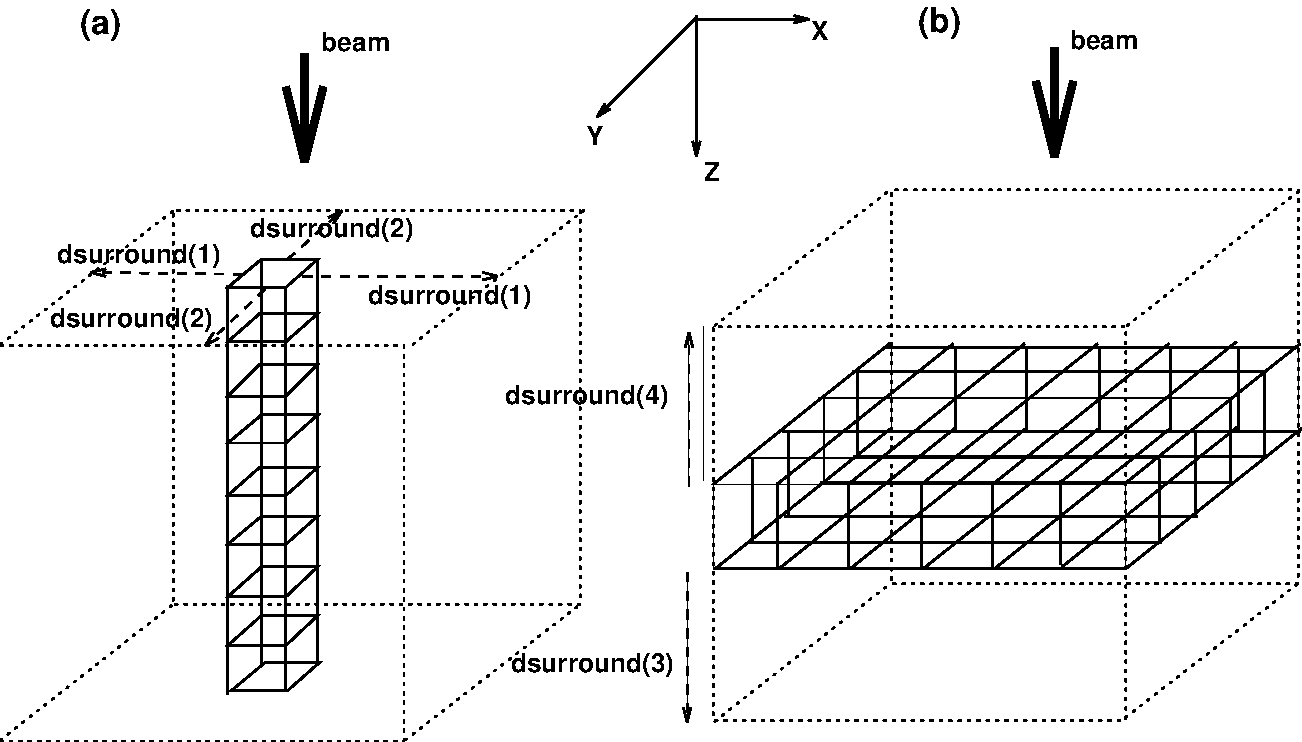
\includegraphics[height=8cm]{figures/dsurround_fig1}
\caption{Two examples of how {\tt dflag} and {\tt dsurround(1...4)} can be used
to
specify a small group of voxels within a larger phantom of the same medium.
In (a) voxels are only specified in a single column for scoring depth-dose,
while the rest of the phantom is defined using {\tt dsurround(1)} and
{\tt dsurround(2)} ({\tt dsurround(3)} and {\tt dsurround(4)} are 0 in this
particular example).  (b) shows voxels specified in a horizontal slice
for scoring the dose profile at a given z value.
In this latter example, the dimensions of the phantom below and above the
slice are defined by {\tt dsurround(3)} and {\tt dsurround(4)} respectively.
{\tt dsurround(1)} and {\tt dsurround(2)} are set to 0 in (b).}
\label{fig_dsurround}
\end{center}
\end{figure}

\lfoot[{{\sffamily \leftmark}}]{{\small Last edited $Date: 2013/09/24 14:49:18 $ }}

Table~\ref{dsurround_table} below shows the results of timing studies
performed using a beam of 10 MeV electrons and a beam
of 6 MV photons incident on a 59x59x10cm water phantom.  For
each beam, 4 cases were simulated: the entire volume filled with 1cm$^{3}$
voxels; 1cm$^{3}$ voxels specified in a column (1x1x10) down
the central (z) axis of the volume (similar to Figure~\ref{fig_dsurround}(a));
1cm$^{3}$ voxels specified in
a vertical slice (1x59x10) through the phantom in the y direction
at x=0; 1cm$^{3}$ voxels specified in a horizontal slice
(59x59x1) through the
phantom at z=2.5cm ($\sim$d$_{max}$)
(similar to Figure~\ref{fig_dsurround}(b)).  In
all cases, simulations were run with and without range rejection.

\begin{table}[htbp]
\caption{Timing results for circular beams of 10 MeV electrons and 6 MV
photons incident on a water phantom.
In all cases, the phantom size is the same (59x59x10 cm$^3$), but the
1x1x1cm$^3$ voxels take up differing parts of the volume (see text).}
\label{dsurround_table}
\begin{tabular}{|p{3cm}|p{3cm}|p{4cm}|p{4cm}|}
\hline
source & number of voxel regions (all 1 cm$^3$) & \multicolumn{2}{|c|}{CPU time (hrs)}\\
\cline{3-4}
       &             & range rejection off & range rejection on \\
\hline
\hline
10 MeV electrons & 59x59x10~~~~~~~ uniform & 0.576 & 0.559 ({\tt ESAVE}=5MeV)\\
\cline{2-4}
(r=10 cm, & 1x1x10 central axis & 0.181 & 0.100 \\
\cline{2-4}
1x10$^{6}$ histories) & 1x59x10 vertical plane & 0.208 & 0.141\\
\cline{2-4}
 & 59x59x1 horizontal plane & 0.345 & 0.300\\
\hline
\hline
6 MV photons & 59x59x10 & 1.623 & 1.525 ({\tt ESAVE}=3MeV)\\
\cline{2-4}
(r=10 cm, & 1x1x10 & 0.785 & 0.479\\
\cline{2-4}
30x10$^{6}$ histories) & 1x59x10 & 0.824 & 0.551\\
\cline{2-4}
 & 59x59x1 & 0.969 & 0.711\\
\hline
\end{tabular}
\end{table}

The table shows that if a depth-dose curve is all that is required, then
specifying voxels only in a 1x1x10cm column can decrease
simulation time by a factor of 5.5 for the electron beam and
a factor of 3 for the photon beam.
In general, the CPU time increases
as the number of voxels specified increases, but orientation of the volume
in which voxels are specified plays a role as well.
The 59x59x1cm horizontal slice
is, relatively, the least efficient use of {\tt dsurround} (saving a factor of
$\sim$2 in CPU time) due to the fact that it has more voxels than the
central-axis phantom and the vertical slice phantom but also due to the fact
that most of the primary and secondary particles from the beam have to be
transported across the
horizontal voxel boundaries defining the slice.  Finally, note that range
rejection is
more efficient when using {\tt dsurround} with a smaller number of
voxels:
turning range rejection on decreases the
simulation time for the case where voxels are only specified in a 1x1x10cm
column by a factor of almost 2, while
its effect on the simulation time when the entire phantom is divided into
voxels is negligible.

Note that this option allows electrons to take much bigger steps in the
{\tt dsurround} regions and this can cause some small inaccuracies unless
the default EGSnrc transport parameters are used.

\section{Pegsless mode}
\indexm{pegsless mode}

As of 2013, DOSXYZnrc can be run independent of the pegs4 cross section data file.  Photon
cross sections had been calculated on the fly since 2006, so the move towards a completely pegsless
version of EGSnrc-based user codes was a logical one.

When running in pegsless mode, all media used in the simulation must be defined
in the {\tt .egsinp} file, between the delimiters, {\tt :start media definition:} and {\tt :stop media definition:}.
{\tt .egsinp} file.  Here, the user has the option of specifying the name of a material data file, containing
\indexm{pegsless mode!material data file}
the compositions, bulk densities, etc, of the media and/or defining media parameters directly in the {\tt .egsinp} file.  The latter method is useful for defining media not included in the material data file or for overriding parameters
in the material data file.  The user also specifies the particle energy limits for cross section calculation:
\indexm{pegsless mode!AE}\indexm{pegsless mode!UE}\indexm{pegsless mode!AP}\indexm{pegsless mode!UP}
{\tt AE} and
{\tt UE} for electrons, {\tt AP} and {\tt UP} for photons.   For more information about the inputs
between the {\tt :start media definition:} and {\tt :stop media definition:} delimiters, including defaults, you are
urged to refer to the BEAMnrc Users Manual\cite{Ro09}.

Pegsless mode is accessible through the DOSXYZnrc GUI by selecting ``Change PEGS4 file'' from the ``File'' menu and
then opting to ``Go PEGSless'' instead of selecting a PEGS4 file.  Once you have done this, a ``Define Media'' button
at the bottom of the main input window becomes active.  Pushing this button will open up a sub-window through
which you have access to the inputs between {\tt :start media definition:} and {\tt :stop media definition:} in
the {\tt .egsinp} file.

\indexm{pegsless mode!running in}
DOSXYZnrc can be run interactively in pegless mode using the command line input:
\begin{verbatim}
dosxyznrc -i inputfile
\end{verbatim}
where {\tt inputfile} is the name of the input file (with no
{\tt .egsinp} extension).

Pegsless batch runs use the command line syntax:
\begin{verbatim}
exb dosxyznrc inputfile pegsless [short|medium|long] [batch=batch_system] [p=N]
\end{verbatim}
This is identical to the syntax of a run with pegs data (see Section~\ref{candrsect} above) but
with the word {\tt pegsless} in place of the name of the pegs data file.

\indexm{pegsless mode!.mederr file}
On termination, pegsless runs output a file, {\tt inputfile.mederr}, containing information about where
the specifications for each medium in the simulation have been read ({\it i.e.} from the material data
file or directly from {\tt inputfile.egsinp}) and various warning messages related to inputs that have
been left blank and have been set to their default values.  The media compositions and settings for other
parameters necessary for calculating cross sections are output to {\tt inputfile.egslst} and
{\tt inputfile.egslog} (for batch runs).

\section{CT Based Phantoms/{\tt ctcreate}}
\indexm{ctcreate}
\indexm{CT!phantoms}

The CT phantom option of DOSXYZnrc allows calculation of dose distributions in
phantoms that are derived from CT data sets. This
allows simulations in realistic anthropomorphic
phantoms. (Please note that the previous sentence does not use the
word patient.)  The creation of CT phantoms from CT data is performed
using the stand-alone code, {\tt ctcreate}.

\indexm{Pinnacle CT}
\indexm{AAPM CT}
\indexm{CT!format!AAPM}
\indexm{CT!format!CADPLAN}
\indexm{CT!format!Pinnacle}
\indexm{CT!format!DICOM}
\indexm{CADPLAN CT}
At this point in time, {\tt ctcreate} supports CT data in DICOM
format (with some restrictions, see below), ADAC
Pinnacle format, and CADPLAN format.
A tool for converting the AAPM CT format into
Pinnacle format is also available.

The process by which CT phantoms are created by {\tt ctcreate}
\indexm{ctcreate}
are outlined here and described in detail in the following sections.

\begin{enumerate}
\item Read in the format of the CT data
\item Read in the CT header parameters (binary or ASCII).
\item Read in the binary CT data.
\item Choose a subset of the CT data set (if desired).
\item Resample the CT data to correspond to volume elements that dose
will be scored in.
\item Convert the CT data to materials and densities for each voxel.
\item Transfer the data via a file to be input to DOSXYZnrc.
\end{enumerate}

\indexm{.egsphant}
\indexm{files!.egsphant}
The relevant CT phantom information
is written into the file, {\tt *.egsphant} (prefix is the same as the
original CT data set name).  A flowchart for the CT phantom code, showing
how it relates to DOSXYZnrc is shown in figure~\ref{fig_ct01}.

Nearly all of the CT phantom functionality takes place outside of
{\tt ctcreate} proper in subroutines.  This
\indexm{ctcreate}
modularity allows for easy changes in the code by ambitious users (for example subroutines for
other CT file formats).  Specifically, this is to provide the user with the
means of reading
their own CT file formats and writing their own dose distribution files
 without rewriting large chunks of
{\tt ctcreate.mortran} and {\tt dosxyznrc.mortran}. This can be accomplished
by creating their
own versions of the subroutines {\tt ReadCT} in {\tt ctcreate.mortran} and
{\tt write\_dose} in {\tt dosxyznrc.mortran}. The
specifications as to what
is required of these subroutines can be found in the codes themselves and
in section~\ref{spec_ReadCT} of this document.

\indexm{CT!coordinate system}
Note that the input CT data set defines the coordinate system for the
calculation, which may be different from the coordinate system of the
accelerator simulation (using BEAM).  For example, for Pinnacle CT
\indexm{Pinnacle CT}
data sets, the Z-axis is typically down the centre of the patient whereas in
the accelerator simulation the Z-axis is the beam's central axis.  This
causes no problems, but must be kept in mind.

\begin{figure}[htbp]
\begin{center}
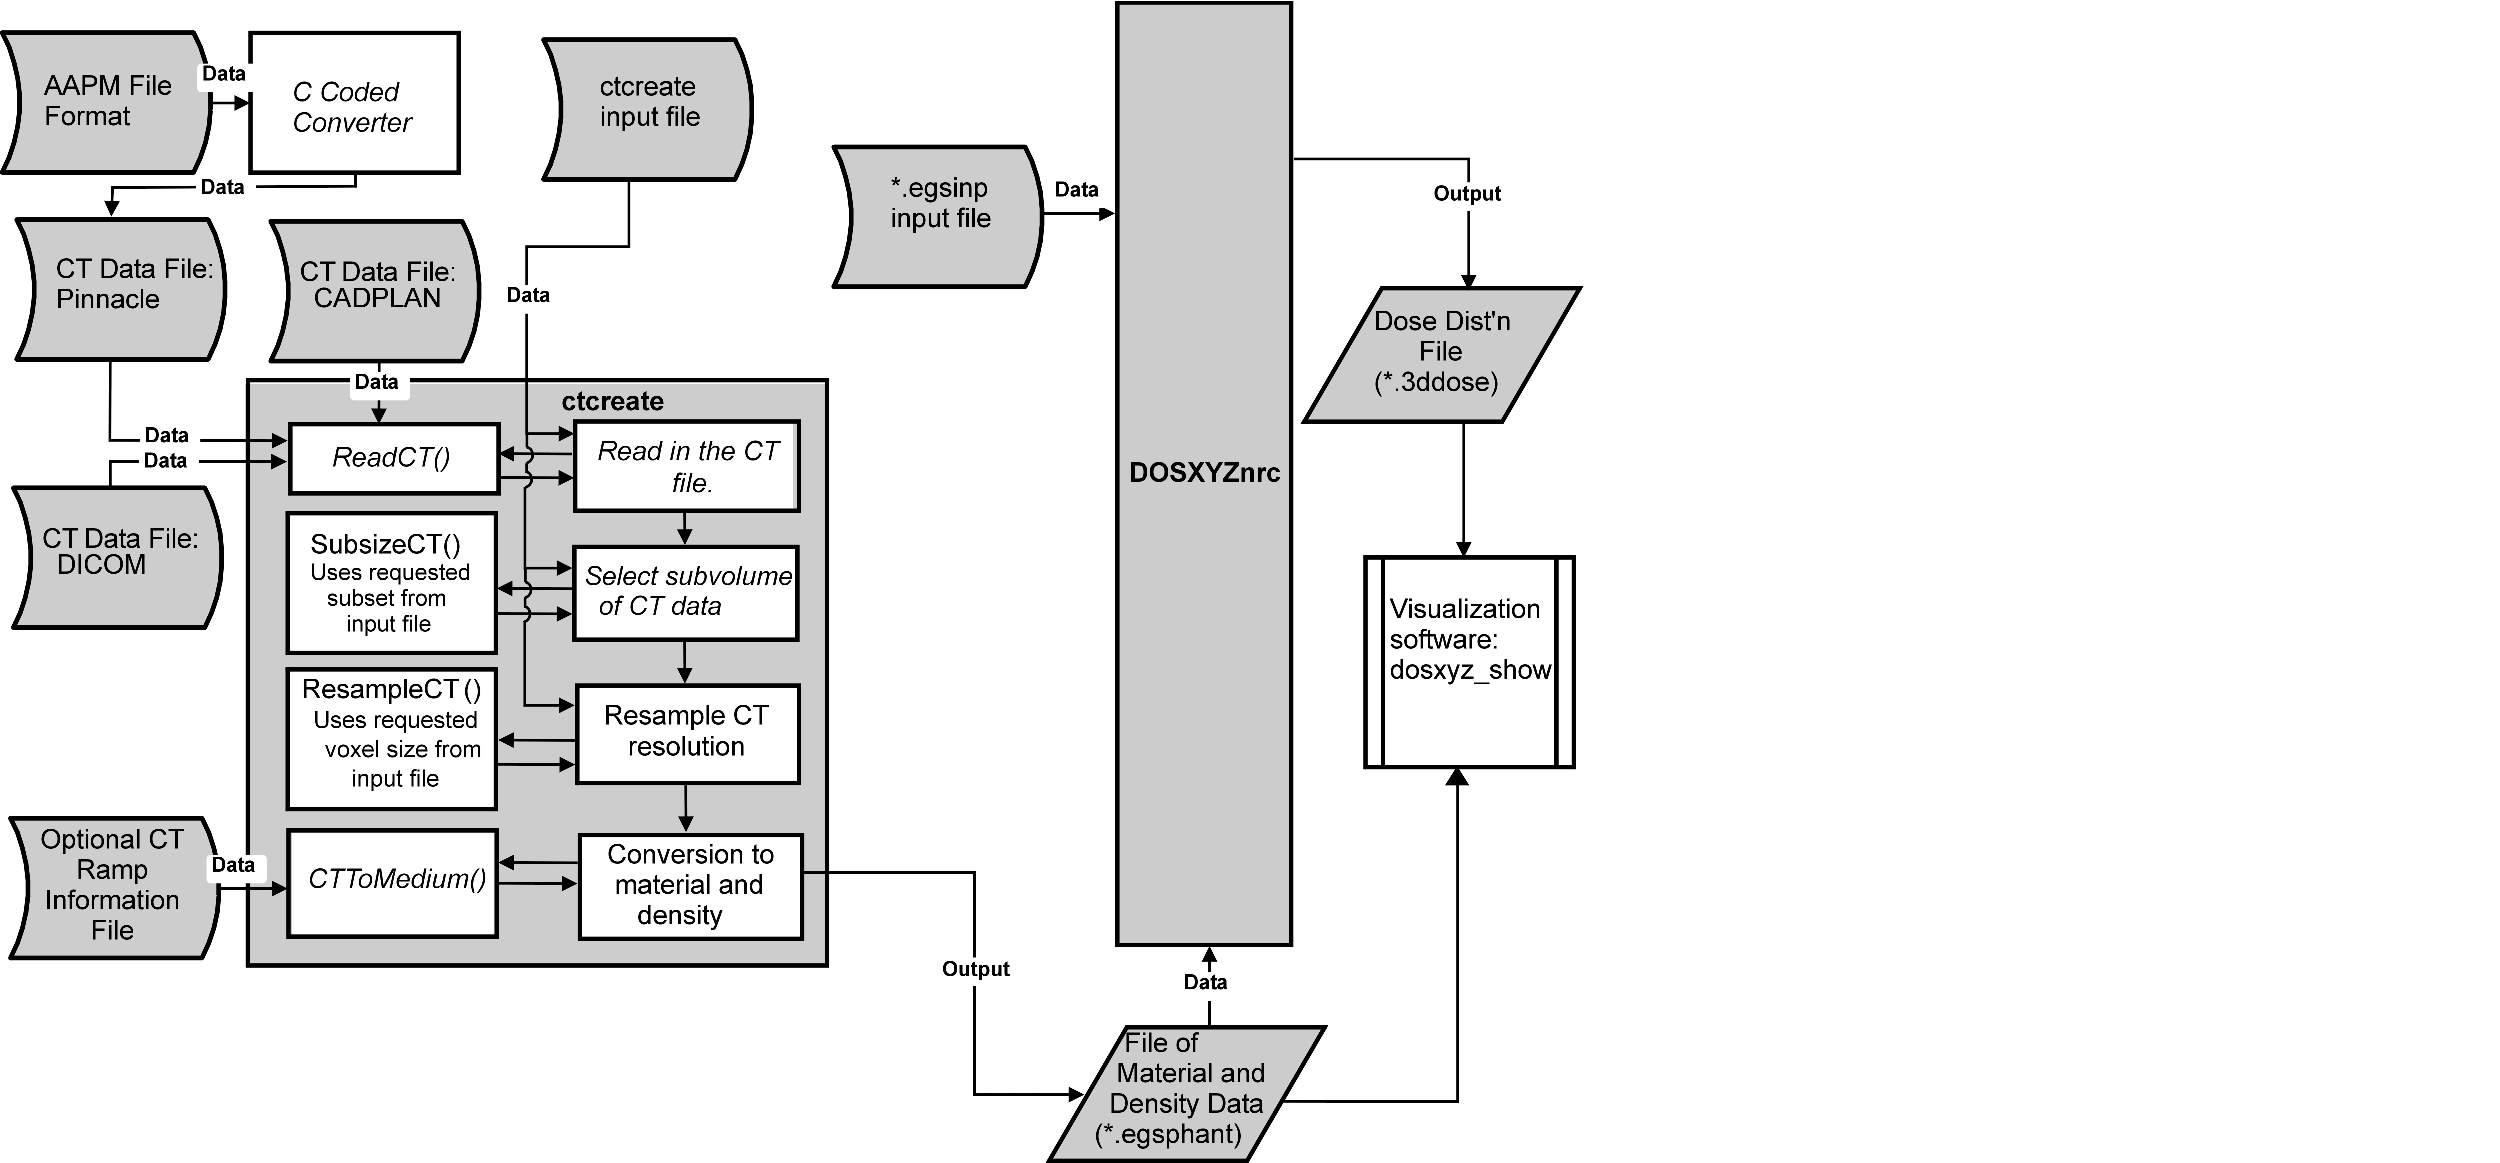
\includegraphics[height=12cm]{figures/ct_fig1}
\caption{A flowchart for use of CT data with  {\tt ctcreate} and DOSXYZnrc. }
\label{fig_ct01}
\end{center}
\end{figure}

\subsection{Using the CT Phantom Option in DOSXYZnrc}

\indexm{CT!option}
\indexm{nmed}
The CT phantom option is used by setting the number of materials,
{\tt nmed} in record 2 of the DOSXYZnrc input file, to zero. This will cause the
program to execute differently than when {\tt nmed} is $>$ 0, and, instead
of geometry, material and density data for the phantom being input explicitly
in the DOSXYZnrc input file,
DOSXYZnrc reads these data from a CT phantom file which has
been created using {\tt ctcreate}.  The input for the
CT and non-CT modes of DOSXYZnrc
are common again after this input (see section~\ref{DOSXYZ_input},
page~\pageref{DOSXYZ_input}).

In short, the input file for DOSXYZnrc is very different if the CT
option is being used.  From section~\ref{DOSXYZ_input} it can be seen
that in CT mode, input records 3-9 in non-CT mode are replaced by
records 3-5, which specify the name of the file containing the CT phantom
data, the transport parameters, and some output parameters.

\subsection{Using {\tt ctcreate}}

\indexm{ctcreate}
\indexm{.egsphant}
\indexm{files!.egsphant}
This section covers the input parameters that {\tt ctcreate} requires
to create a {\tt *.egsphant} CT phantom file that can then be read in and
used by DOSXYZnrc.

It is fairly simple to obtain a
CT phantom from the CT data set since all the required material and geometry
information is contained in the data set.
The additional information that the user is required to provide
are the CT data format, the name of the file containing either the header
info (Pinnacle) or containing the names of the actual CT data files (CADPLAN
and DICOM),
voxel dimensions for the phantom. The user can also select a subset of the full
CT data and specify their own CT ramp (ie function for converting
\indexm{CT!ramp}
CT data to the densities and materials required for the DOSXYZnrc phantom).  Input
of a custom CT ramp is highly recommended.

The following are the input parameters for {\tt ctcreate}.  This description
is found at the beginning of the {\tt ctcreate.mortran} code.
\indexm{ctcreate!input parameters}
\begin{small}
\input{inputs/ctcreate.inp}
\end{small}
\indexm{running ctcreate}

Parameters may be input interactively, by typing:

{\tt ctcreate}

and responding to the prompts;  or stored in an input file
and {\tt ctcreate} run with the input file by typing:

{\tt ctcreate inputfilename}

{\tt ctcreate} input parameters are described in more detail in the subsections below.

\subsubsection{{\tt ctformat}}
\indexm{CT!format}
The first input required by {\tt ctcreate} is the format of the
CT data.  Currently, {\tt ctcreate} supports {\tt Pinnacle}, {\tt
CADPLAN} and {\tt DICOM} formats.
If the data is in AAPM format, then it can be converted to Pinnacle format
using the code
{\tt \$OMEGA\_HOME/progs/ctcreate/CT/AAPM/aapm2pinnacle}
\indexm{aapm2pinnacle}
\indexm{AAPM format}
\indexm{Pinnacle format}
\indexm{CADPLAN format}

\subsubsection{{\tt CTFilename}}
\indexm{CT!data file}
\indexm{CTFilename}
{\tt CTFilename} is the full name of a file, the contents of which depend
on the CT data format:
\begin {description}
\item [Pinnacle format]
\indexm{Pinnacle CT}
{\tt CTFilename} is the full name of the header file of the CT data set
(including the {\tt .header} extension).
The code
will read in all the information that it requires from this file before
moving on to read in the entire binary data file (which has an assumed
extension {\tt .img} and the same prefix as the header file).
  %A sample Pinnacle header file is shown in the next section of this document.
\item [CADPLAN and DICOM formats]
\indexm{CADPLAN CT}
\indexm{DICOM CT}
{\tt CTFilename} is the full name ({\it i.e.} including directory path)
of a file containing the full names of the
individual CT data files (1 file/image slice).  The file names MUST appear
in order of increasing Z position of the slice.
\end{description}

\indexm{.egsphant}
\indexm{files!.egsphant}
On output, the CT phantom will be named:\\
{\tt CTFilename(minus .header extension if using Pinnacle format).egsphant}\\

\subsubsection{{\tt xctsubmin,xctsubmax,yctsubmin,yctsubmax,zctsubmin,zctsubmax}}
\indexm{CT!sub-volume}
\indexm{xctsubmin}
{\tt xctsubmin},{\tt xctsubmax}, {\tt yctsubmin}, {\tt yctsubmax},
{\tt zctsubmin},
and {\tt zctsubmax} are used to create six planes which describe a cube.
The subsection of the original CT data contained in this cube will
be used to create the CT phantom. In this
manner only the portion of interest in the original CT data is used in
the simulation.  This allows the particle simulation
to be performed at a higher resolution than if the calculation used the
entire CT volume, and allows the user to trim some of the air that surrounds
a typical CT image from consideration in the phantom.  Note that if the
sub-volume selected by the user does not fit on an integer number of voxels
from the original CT data, then the sub-volume will automatically be expanded
until it does so.

\subsubsection{{\tt xyz\_xthickness,xyz\_ythickness,xyz\_zthickness}}
\indexm{CT!phantom voxels}
\indexm{voxel size}
\indexm{xyz\_xthickness}
The third line of the input to {\tt ctcreate} is the
spatial resolution that the user requires for the simulation.
{\tt xyz\_xthickness}, {\tt xyz\_ythickness}, {\tt xyz\_zthickness}
are the 3 dimensions of the voxels to be used in the CT phantom.
The maximum voxel dimension in a given direction is
the distance between the planes delimiting the subset of the CT data
to be used in that direction (see previous section).
The minimum voxel dimension in a direction is the distance between
the planes delimiting the subset of CT data in that direction divided
by the maximum number of voxels allowed in that direction (set at
compilation).
{\tt ctcreate} will alert the user when dimensions less than the minimum
or greater than the maximum are input.  Note that, if necessary, the voxel
dimensions will always be increased to fit an integer number of DOSXYZnrc
voxels on the CT sub-volume selected by the user.

\subsubsection{{\tt num\_material}, {\tt material\_ct\_lower\_bound}, and other CT ramp inputs}
\indexm{CT!ramp}

{\tt num\_material} is the
number of materials in the ramp function used
to convert CT number in each voxel to material and density.
If this is set to zero then a
default CT ramp is used in the conversion. The default ramp
is shown in Figure~\ref{fig_ct02} and in the sample input file given in the next section.
{\tt material\_ct\_lower\_bound} defines the lowest CT number of the first ramp
({\it i.e.} the lowest CT number for material  1).  If the default ramp is used, then {\tt material\_ct\_lower\_bound} defaults
to -1024, which is typically the minimum CT number for air in DICOM format data.

If {\tt num\_material} $>$0 then
the CT ramp is read from
the input file.  For each medium in the ramp, there are
two lines of input. \indexm{CT!ramp}
The first of these lines is the name of the material
({\tt material\_name}) which must be identical to a material in the
{\tt PEGS4} material data file being used in the DOSXYZnrc simulation.
The second line specifies the maximum CT number for the medium, {\tt material\_ct\_upper\_bound},
the minimum density of the medium, {\tt material\_density\_lower\_bound}, and the maximum
density of the medium,
{\tt material\_density\_upper\_bound}. Note that the ramp is assumed to be continuous
in CT number.  Thus, for material {\tt n}, {\tt material\_density\_lower\_bound(n)} corresponds
to a CT number of {\tt material\_ct\_upper\_bound(n-1)} (or the overall
minimum CT no. of the ramp, {\tt material\_ct\_lower\_bound}, if
{\tt n}=1), and {\tt material\_density\_upper\_bound(n)} corresponds to
{\tt material\_ct\_upper\_bound(n)}.
Also note that the ramp must be input in order of
increasing {\tt material\_ct\_upper\_bound}.

The CT ramp is then used to determine the medium and density in each voxel of the CT data.
\indexm{CT!ramp}
If a voxel's CT number is $\leq$ {\tt material\_ct\_upper\_bound(n)} and
$>$ \\
{\tt material\_ct\_upper\_bound(n-1)} (or {\tt material\_ct\_lower\_bound} if
{\tt n}=1)
then it is assigned medium {\tt n}. The density is then calculated using a linear
interpolation between the medium's density limits:
\begin{align}
{\tt r}&{\tt hor}_{i,j,k} = {\tt material\_density\_lower\_bound(n)} \nonumber \\
             &+\left(\frac{{\tt material\_density\_upper\_bound(n)}-
 {\tt material\_density\_lower\_bound(n)}}
{{\tt material\_ct\_upper\_bound(n)}-
 {\tt material\_ct\_upper\_bound(n-1)}}\right)        \\
        &*({\tt CT}_{i,j,k}-{\tt material\_ct\_upper\_bound(n-1)}) \nonumber
\end{align}

The default ramp is shown in Figure~\ref{fig_ct02}. This is a modified version of
\indexm{CT!ramp}
a CT ramp given in Kawrakow et al\cite{Ka96a}.  Note that this ramp has been
optimized for typical DICOM format data, where the lowest CT number for air
{\tt material\_ct\_lower\_bound} is -1024.

If the CT number in a voxel is less than {\tt material\_ct\_lower\_bound} then
the medium in that voxel is set to vacuum with density zero.
Those voxels with CT numbers above the
last material's upper CT number ({\tt material\_ct\_upper\_bound(num\_material)})
will have the density set to the maximum
density for the last material.

\begin{figure}[H]
\begin{center}
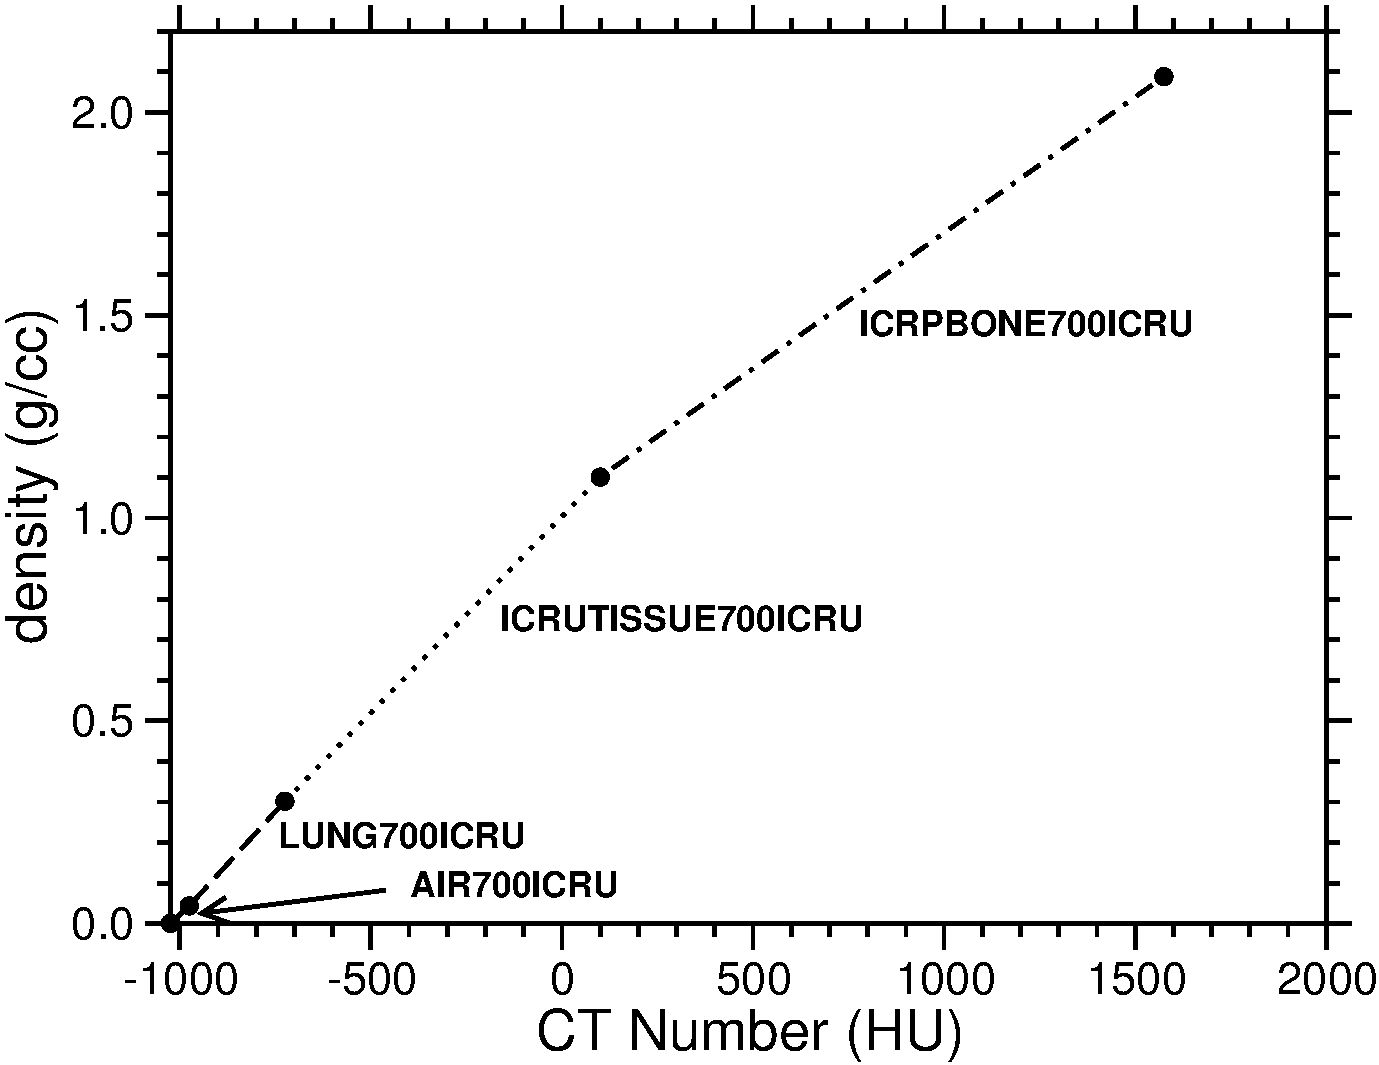
\includegraphics[width=10.5cm]{figures/CTramp}
\caption{The default ramp for converting CT values to material and
density in {\tt ctcreate} modified from Kawrakow et al\cite{Ka96a}.}
\label{fig_ct02}
\end{center}
\end{figure}
\indexm{CT!ramp}

The default CT ramp may be suitable for displaying a {\tt .egsphant} file
using {\tt dosxyz\_show}\cite{Ka98} and for example calculations.  However,
we strongly recommend that you explicitly enter your own CT ramp function
for more detailed simulations, since the CT ramp is
dependent upon the imager and the data acquisition method.

\subsection{Sample {\tt ctcreate} CT Phantom Input File}
\indexm{ctcreate!sample input}
Table~\ref{ctinpex} shows an example {\tt ctcreate} input file, and
a sample DOSXYZnrc input file (excluding EGSnrc inputs)
which uses the CT phantom data from {\tt ctcreate}.

\vspace*{-0.5cm}
\begin{table}[htbp]
%\begin{tabular}{|p{8cm}p{7.7cm}|}
\caption{Sample input files for {\tt ctcreate} and DOSXYZnrc}
\begin{tabular}{|p{7cm}p{8.7cm}|}
\hline
\bf{Input Parameter} & \bf{Description of input fields.} \\
\multicolumn{2}{|c|}{\bf for {\tt ctcreate}      } \\
{\tt DICOM} & CT data is in DICOM format \\
{\tt CTfname} & in DICOM format, this is the name of a file containing the names of the individual image slices (in order
of increasing Z).
\\
%\hline
{\tt -17.64,17.64,-17.64,17.64,-0.7,4.3}
&
The subvolume of the CT data set
that is to be used for the phantom.
\\
%\hline
{\tt 1.0, 1.0, 1.0 }
&
The phantom voxel size.
\\
%\hline
{\tt 4, -1024}
&
{\tt num\_material}, {\tt material\_ct\_lower\_bound}.
If {\tt num\_material}=0
the default ramp will be used.
The default values are
listed explicitly in this example.
\\
%\hline
{\tt AIR700ICRU }
&
The material\_name for the first material.
\\
%\hline
{\tt -974,0.001,0.044}
&
CT ramp parameters for the first material:\\
&{\tt  material\_ct\_upper\_bound}, \\
&{\tt material\_density\_lower\_bound},\\
&{\tt material\_density\_upper\_bound}
\\
%\hline
{\tt LUNG700ICRU }
&
The material name for the second material.
\\
%\hline
{\tt -724,0.044,0.302}
&
The ramp parameters for the second material. \\
%\hline
{\tt ICRUTISSUE700ICRU} & The material name for the third material.
\\
%\hline
{\tt 101,0.302,1.101} & The ramp parameters for the third material.
\\
%\hline
{\tt ICRPBONE700ICRU} & The material name for the fourth material.
\\
%\hline
{\tt 1976,1.101,2.088} & The ramp parameters for the fourth material.
\\
\hline
\multicolumn{2}{|c|}{\bf for DOSXYZnrc} \\
%\hline
{\tt Sample CT Input File } & Title of the simulation and phantom. \\
%\hline
0 & {\tt NMED } - If this is zero the code switches to CT\_Phantom mode. \\
%\hline
{\tt CTfname.egsphant} & The name of the CT phantom file.\\
{\tt 0.7,0.01,5.0} & {\tt ECUTIN}, {\tt PCUTIN}, {\tt SMAX} (dummy inputs)\\
{\tt 1,0,1} & {\tt zeroairdose}, {\tt doseprint} and {\tt MAX20} \\
%\hline
{\tt -1,0,-1.25,1.25,-2.25,2.25,90.0,} & The source description record.
At this point the \\
{\tt 90.0,0.0} &CT phantom input meets up with the manual\\
& phantom inputs.
\\
%\hline
{\tt 0}
&
monoenergetic particle spectrum.
\\
%\hline
{\tt 20.0 }
&
particle energy.
\\
%\hline
{\tt 100,0,500.,7,3,100.,0,0,0,1,5.0,} & Monte Carlo information (note range rejection \\
\hspace*{1cm}{\tt 0,0,0,0}&below 5MeV).  \\
%\hline
\hline
\end{tabular}
\label{ctinpex}
\end{table}

\subsection{Location of {\tt ctcreate} and How to Compile It}
\label{comp_ctcreate}
{\tt ctcreate.mortran} and related files
(see section~\ref{filesect} for a complete list)
\indexm{ctcreate!installation}
reside in the subdirectory {\tt \$OMEGA\_HOME/progs/ctcreate}.
Normally, it is compiled as part of the OMEGA/BEAM installation
(see the BEAMnrc Manual\cite{Ro04a} for installation instructions), however
it can be compiled separately by going into this directory and
typing {\tt make}.

\subsection{{\tt ReadCT()} Subroutines}
\label{spec_ReadCT}
\indexm{ReadCT}
\indexm{CT!format!AAPM}
\indexm{CT!format!CADPLAN}
\indexm{CT!format!DICOM}
\indexm{CT!format!Pinnacle}
{\tt ReadCT} is the most important subroutine in {\tt ctcreate}.  It handles
the reading in of header information and binary CT data.  Currently, there
are three {\tt ReadCT} subroutines within {\tt ctcreate}, one for each of the CT formats
supported: {\tt ReadCT\_Pinnacle} for Pinnacle, {\tt ReadCT\_CADPLAN}
for CADPLAN data and {\tt ReadCT\_DICOM} for DICOM data.

\subsubsection{{\tt ReadCT\_Pinnacle}}
\indexm{ReadCT\_Pinnacle}
\indexm{CT!format!Pinnacle}

{\tt ReadCT\_Pinnacle} is contained
within the {\tt ctcreate.mortran} file and calls
other subroutines and functions in this file:
\begin{description}
\indexm{ReadReal}
\indexm{ReadInt}
\indexm{read\_ct\_data}
\indexm{swap\_bytes}
\item[{\tt ReadReal}] Reads real values from the image header ({\tt .header}) file.
\item[{\tt ReadInt}] Reads integer values from the header file.
\item[{\tt read\_ct\_data}] Reads binary CT data from the image ({\tt .img})
file.
\indexm{swapping bytes}
\item[{\tt swap\_bytes}] Swaps bytes of CT data if there is a
byte order mismatch between the data and the machine you are using.
\end{description}

Note that in Pinnacle format CT numbers are $>$ 0.  Thus, the default CT ramp
in {\tt ctcreate} cannot be used to convert CT numbers to media and densities.
The example {\tt ctcreate} inputfile, {\tt \$OMEGA\_HOME/progs/ctcreate/ctcreate\_examples/CT\_create.inp}
(used in Lab VI in the BEAMnrc Workshop), is used to convert Pinnacle format data and
contains a custom CT ramp which is just the default ramp shifted up by 1025 HU.

\subsubsection{{\tt ReadCT\_CADPLAN}}
\indexm{ReadCT\_CADPLAN}
\indexm{CT!format!CADPLAN}
{\tt ReadCT\_CADPLAN} is also contained
within the {\tt ctcreate.mortran} file.
Unlike {\tt ReadCT\_Pinnacle}, {\tt ReadCT\_CADPLAN} is a self-contained subroutine.
Byte swapping is not required since single bytes are read at a time.


\subsubsection{{\tt ReadCT\_DICOM.c}}
\indexm{CT!format!DICOM}
\indexm{ReadCT\_DICOM}
{\tt ReadCT\_DICOM.c} is a separate C routine whose object file is linked
to {\tt ctcreate} at compile time.  {\tt ReadCT\_DICOM.c} is automatically
compiled when you {\tt make} ctcreate.
{\tt ReadCT\_DICOM.c} requires the C header file {\tt tags\_ct.h}, which
defines hexadecimal tags, or labels, for the DICOM data.  These tags
are defined in the DICOM standard, and if the user modifies
{\tt ReadCT\_DICOM.c} to deal with additional tags, then these can
be added to the {\tt tags\_ct.h} file.
Currently,
{\tt ReadCT\_DICOM} assumes
\indexm{little endian byte order}
\indexm{big endian byte order}
the DICOM data has been collected on a machine with little endian byte order
(ie compatible with Linux), however, if the data was collected on a machine
with big endian byte order, you must go into {\tt ReadCT\_DICOM.c} and
change the line:
\indexm{DICOM\_ENDIAN}
\begin{verbatim}
#define DICOM_ENDIAN 1
\end{verbatim}
to:
\begin{verbatim}
#define DICOM_ENDIAN 0
\end{verbatim}
and recompile {\tt ctcreate}.  The endianness of the machine you
are running {\tt ctcreate} on is automatically detected by
{\tt ReadCT\_DICOM} and then bytes are swapped if necessary.

The DICOM format is known to vary from imager to imager and institute
to institute.  Thus, we cannot guarantee that {\tt ReadCT\_DICOM} will
work with your images without modification.  As a minimum,
the current version of {\tt ReadCT\_DICOM} requires the following
information in the image (slice) header(s):
\begin{enumerate}
\item Number of rows (data tag {\tt 0x00280010}).  This defines the number of voxels in the X-direction.
\item Number of columns (data tag {\tt 0x00280011}). This defines the number of voxels in the Y-direction.
\item Pixel spacing (data tag {\tt 0x00280030}).  Defines the X- and Y-dimensions of the voxels.
\item Image position (data tag {\tt 0x00200032}). Defines the (X,Y,Z) of the centre of the first voxel.  The position
of the first slice (slice with lowest Z) is used to determine the X-, Y- and
Z-offset (starting position) of the CT data, and the Z-positions of the first two slices are used
to established voxel Z-dimension ({\it i.e.} slice thickness).
The Z-positions of slices as read from the header are also used to
sort slices in order of increasing Z, in case the user has not already done so
in the file containing the slice names.
\item A pixel data tag ({\tt 0x7fe00010}) indicating the size of the data array in bytes.  This tag must appear last in the
header, immediately preceding the CT data itself.
\end{enumerate}

{\tt ReadCT\_DICOM} assumes slices are contiguous in Z.  Thus, once the Z-position of the first slice and slice thickness (Z-dimension of voxels) are
established, {\tt ReadCT\_DICOM} positions subsequent slices so that there are no gaps
or overlaps between them.  A warning message is output if the Z-position of
a slice determined by {\tt ReadCT\_DICOM} does not equal the Z-position
of the slice as read from the image position in its header.

We note that {\tt ReadCT\_DICOM.c} has limited flexibility in terms of slice
layout, and it has not been
tested on all possible variations of the DICOM format.  Therefore, if you
require more flexibility or are having trouble converting your DICOM files, you
are strongly urged to either modify {\tt ReadCT\_DICOM} or use your own
stand-alone routine for converting DICOM images to {\tt .egsphant} files.

\indexm{Nick Reynaert}
The initial version of {\tt ReadCT\_DICOM.c} was provided by Nick Reynaert at the University of Ghent.

\subsubsection{Generic {\tt ReadCT}}
\indexm{ReadCT!Generic}

Essentially, {\tt ReadCT} is the subroutine or stand-alone
code which the user will have to
\indexm{ReadCT specs}
customize or program from scratch to deal with any CT format not currently
handled.  The structure and number of subroutines within {\tt ReadCT} is
largely a matter of the programmer's taste.  However, if {\tt ReadCT} is
to be included in {\tt ctcreate} (or linked as an object file when compiling
{\tt ctcreate}), it must
pass certain essential data back to {\tt ctcreate}.   An example call to
a generic {\tt ReadCT} routine is:

\noindent {\tt Subroutine ReadCT(fname,asize,ctdata,offset,vsize,error)}

\noindent where {\tt fname} is a character string containing the name of the
particular CT data set.  The essential CT data returned to {\tt
ctcreate} are:
\begin {description}
\item [{\tt asize(3)}]  An array returning the number of CT voxels in the
                     x,y,z directions.
\item [{\tt vsize(3)}]  An array returning the dimensions of the CT voxels

\item [{\tt offset(3)}] An array returning the lower bounds of the CT data
                      in the x,y,z directions in cm.
\item [{\tt ctdata(\$CTIMAX,\$CTJMAX,\$CTKMAX)}] A 3-D integer array
           returning the CT data (Hounsfield numbers).  In {\tt ctdata},
    {\tt x}$\rightarrow${\tt i},
    {\tt y}$\rightarrow${\tt j},
    {\tt z}$\rightarrow$ {\tt k}, so that {\tt ctdata(i,j,k)} is
    equal to the Hounsfield number in the voxel with lower bounds
    {\tt x=offset(1)+(i-1)*vsize(1)}, {\tt y=offset(2) +} {\tt (j-1)*vsize(2)},
    {\tt z=offset(3)+} {\tt (k-1)*vsize(3)} and
    upper bounds {\tt x=offset(1)+} {\tt i*vsize(1)},
    {\tt y=offset(2)+} {\tt j*vsize(2)}, {\tt z=offset(3)+} {\tt k*vsize(3)}
\item [{\tt error}] Returns the error status of the CT read operation.
                    Currently not used.
\end {description}

\subsection{Description of the {\tt *.egsphant} File}
\label{egsphantsect}
\indexm{.egsphant}
\indexm{files!*.egsphant}
The {\tt *.egsphant} file output by {\tt ctcreate} or by DOSXYZnrc itself
is an ASCII file
containing the following information necessary for DOSXYZnrc to simulate
the CT phantom and for the display program, {\tt dosxyz\_show}\cite{Ka98},
to display the density information:
\begin{enumerate}
\item The number of media in the phantom
\item The names of the media
\item The {\tt ESTEPE} value for each medium (now a dummy input)
\item The number of voxels in the X, Y and Z directions
\item A list of the voxel boundaries in the X direction
\item A list of the voxel boundaries in the Y direction
\item A list of the voxel boundaries in the Z direction
\item For each Z slice, an X-Y array containing the medium
      number in each voxel
\item For each slice in the Z direction, an X-Y array containing the densities
      in each voxel
\end{enumerate}
\vspace*{-0.3cm}
In addition to passing the necessary medium information to DOSXYZnrc, the X-Y
arrays of medium numbers (item 8 above) provide a rough slice-by-slice
view of the CT phantom.  A sample X-Y array of medium numbers from one slice of a CT phantom derived
from a lung image is shown below (hold at a distance, and raw data on
screen is easier to see):

\input{inputs/mednoarray.inp}

The user can use these slice-by-slice views to
determine whether the CT data is being read in correctly by {\tt ReadCT}
or to verify that the sub-volume of the original CT data selected
includes the physiology of interest.

\subsection{Files and Macros for implementation.}
Below is a short description of the files and macros required to compile
and run {\tt ctcreate} and DOSXYZnrc with CT phantoms.
\indexm{ctcreate!files and macros}

\begin{description}
\item[{\tt dosxyznrc\_user\_macros.mortran}]
{\tt ctcreate} uses the version stored in\\
{\tt \$HEN\_HOUSE/user\_codes/dosxyznrc}
to obtain {\$IMAX}, {\$JMAX} and {\$KMAX},
the maximum X, Y and Z dimensions of the CT phantom allowed in DOSXYZnrc.

\item[{\tt \$CTIMAX, \$CTJMAX, \$CTKMAX }]
Macros defining the maximum X, Y and Z dimensions of the CT data to be read in.
These macros are in {\tt ctcreate.mortran}

\item[{\tt lnblnk1.mortran}] {\tt MORTRAN} macro to provide the
FORTRAN {\tt lnblnk} function for Linux, rs6000 and HP9000 machines.
{\tt ctcreate} makes extensive use of this function and DOSXYZnrc uses it
in CT phantom mode.  It
is read from the {\tt \$HEN\_HOUSE/src} directory
\end{description}

\section{Known Bugs/Restrictions}

A resumed run that uses a phase space source with particle recycling will
not produce dose/uncertainty results identical to a single run with
the same total number of histories.  This is because the last particle
used before resuming may not have been recycled the full
{\tt NRCYCL} times, and resuming automatically skips to the next particle.
Results will agree within uncertainty, however.

It is recommended that when using the built-in parallel processing
functionality you do not resume parallel runs that use
a phase space source.  In this case, parallel jobs have lost track
of which chunks of the phase space source they were using in the
original run and the uncertainty analysis after recombining the
resumed runs will not take into account correlations due to reusing
chunks of the phase space source.

\section{Acknowledgments}

Charlie Ma was a major contributor to the DOSXYZ code and was the senior
author of the original DOSXYZ manual. Since he is not directly involved
with DOSXYZnrc, he is no longer an author of the manual, but his
contribution to the original code while he was at NRC still plays a
significant role in the current version.


A variety of people have contributed various pieces of code to the
DOSXYZnrc program.  We wish to thank: Julie Zachman of UW for providing
the aapm2pinnacle tool; Daryoush Sheikh-Bagheri for developing PAW
macros for displaying dose distributions and CT files; Geoff Zhang and
Daryoush again for extensive use of the code and drawing our attention
to bugs; Alex Bielajew for early work on the code; Marc Lauterbach and
Joerg Lehmann for initial coding to read CADPLAN CT data sets.
We also wish to thank Paul Reckwerdt for his work on the original code to
read Pinnacle CT data sets; Mark Holmes for his extensive work on reading
CT data and for coding the correlated sampling routines\cite{Ho99}; Brian
Geiser for the BTREE beam modeling method\cite{Ge95}.  \indexm{CADPLAN CT}

\begin{latexonly}
\section{References}
\end{latexonly}
\renewcommand{\rightmark}{References}
\indexm{references}
\typeout{****references start here}
\setlength{\baselineskip}{0.4cm}
\vspace*{-1cm}
\bibliography{../irs}
\bibliographystyle{unsrt}


\newpage
\setlength{\baselineskip}{0.5cm}

%%%%%%%%%%%%%%%%%%%%%%%%%%%%%%%%%%%%%%%%%%%%%%%%%%%%%%%%%%%%%%%%%%%%%%%%%%%%%%%
%
%  EGSnrc dosxyznrc manual
%  Copyright (C) 2021 National Research Council Canada
%
%  This file is part of EGSnrc.
%
%  EGSnrc is free software: you can redistribute it and/or modify it under
%  the terms of the GNU Affero General Public License as published by the
%  Free Software Foundation, either version 3 of the License, or (at your
%  option) any later version.
%
%  EGSnrc is distributed in the hope that it will be useful, but WITHOUT ANY
%  WARRANTY; without even the implied warranty of MERCHANTABILITY or FITNESS
%  FOR A PARTICULAR PURPOSE.  See the GNU Affero General Public License for
%  more details.
%
%  You should have received a copy of the GNU Affero General Public License
%  along with EGSnrc. If not, see <http://www.gnu.org/licenses/>.
%
%%%%%%%%%%%%%%%%%%%%%%%%%%%%%%%%%%%%%%%%%%%%%%%%%%%%%%%%%%%%%%%%%%%%%%%%%%%%%%%
%
%  Authors:         Blake Walters, 2001
%                   Iwan Kawrakow, 2001
%                   Dave Rogers, 2001
%
%  Contributors:    Frederic Tessier
%                   Marc-Andre Renaud
%
%%%%%%%%%%%%%%%%%%%%%%%%%%%%%%%%%%%%%%%%%%%%%%%%%%%%%%%%%%%%%%%%%%%%%%%%%%%%%%%


%Some conventions:
%	DOSXYZnrc, the code name is in capitals, standard font
%	all file names are in {\tt   }  or \verb+    +
%	the code name ctcreate is also {\tt ctcreate}
%
\documentclass[12pt,twoside]{article}      %twoside messes up indexm and keys
%\usepackage{showkeys}   %this messes up some split commands

%\usepackage[breaklinks]{hyperref}
\usepackage{hyperref}
\hypersetup{colorlinks=true, citecolor=blue, linkcolor=blue, filecolor=blue, urlcolor=blue}
\urlstyle{same}

\usepackage{html}
\usepackage{fancyhdr}
\usepackage{amsmath}  %changed from amstex which is now obsolete
\usepackage{float}
\usepackage{rotating}
\usepackage{enumitem}
\setlength{\textwidth}{16.51cm}
\setlength{\textheight}{23.5cm}
\setlength{\oddsidemargin}{0.0in}
\setlength{\evensidemargin}{0.0in}
\setlength{\topmargin}{-1.5cm}
\setlength{\parindent}{1.5em}
\setlength{\topsep}{0ex}
\setlength{\itemsep}{0ex}

\newcommand{\Co}{$^{60}$Co}
\newcommand{\parsp}{~\hspace*{1.5em}}
\setlength{\parskip}{0.1in}
\setlength{\baselineskip}{0.4in}
\newcommand{\head}[1]{\begin{center}\begin{Large}{\bf #1}
                                              \end{Large}\end{center}}
\newcommand{\cen}[1]{\begin{center} #1 \end{center}                   }
\newcommand{\etal}{{\em et.al.}}
\newcommand{\etc}{{\em etc}}

%*** UW does not have the following files and needs them
%DR  You must have this to use latex2html

\renewcommand{\footrulewidth}{0.4pt}
\renewcommand{\headrulewidth}{0.4pt}

%\rfoot[{\sffamily {\rightmark}}]{{\sffamily {\rightmark}}}

\lhead[{\sffamily \thepage~}]{{\sffamily NRCC Report PIRS-794(revB) }}
\rhead[{\sffamily DOSXYZnrc Users Manual}]{{\sffamily ~\thepage}}
\rfoot[{\sffamily \rightmark}]{{\sffamily \leftmark}}
\lfoot[{{\sffamily \leftmark}}]{{\small Last edited $Date: 2013/09/24 14:49:18 $
}}

\cfoot{}

\makeindex
\newcommand{\indexm}[1]{\index{#1}}
%Use the above for final runs  - following is for drafting
%\newcommand{\indexm}[1]{\marginpar{{\tiny {\sf #1}}}\index{#1}}
%above doesn't work well with twosided

\renewcommand{\refname}{}


\begin{document}

\begin{htmlonly}
For information about the authors and/or institutions involved with this
work, use the links provided in the author list.\\
\begin{rawhtml}
<br><br>
\end{rawhtml}

\begin{rawhtml}
<br><br>
\end{rawhtml}

Postscript versions of the entire paper are available.  You may have to
download the compressed version to disk, uncompress or gunzip them and
then read or print them.
\htmladdnormallink{(pdf version 2.0 Mb)}{pirs794.pdf}
\htmladdnormallink{(uncompressed version 4.5 Mb)}{pirs794.ps}
\htmladdnormallink{(gzip version 2.2 Mb)}{pirs794.ps.gz}
\begin{rawhtml}
<br>
\end{rawhtml}

Use the Up button to get back to this page from within the document.
\begin{rawhtml}
<BR> <HR> <P>
\end{rawhtml}
\copyright
Copyright 1995-2021, National Research Council of Canada
Ottawa
\begin{rawhtml}
<BR> <HR> <P>
\end{rawhtml}
\end{htmlonly}

\pagestyle{empty}

\vspace*{-2cm}

\title{DOSXYZnrc Users Manual}
\begin{center}
{\sffamily \bfseries \Huge DOSXYZnrc Users Manual \vspace{5mm}\\}
\begin{large}
B. Walters, I. Kawrakow and D.W.O. Rogers \\
\end{large}
%\vspace*{0.3cm}
{Ionizing Radiation Standards}\\
{National Research Council of Canada,}
Ottawa K1A 0R6\\

Printed: \today  \vspace{7mm}\\
\hfill NRCC Report {\sf PIRS-794revB       }\\

%\maketitle
\vspace*{-2cm}
\begin{htmlonly}       %%%%%%%%%%%%%%%%%%%%%%%%%%%%%%%%%%%%%%%%%%%%%%
\begin{rawhtml}
<center>
\end{rawhtml}
\end{htmlonly}       %%%%%%%%%%%%%%%%%%%%%%%%%%%%%%%%%%%%%%%%%%%%%%
\begin{figure}[H]
\begin{center}
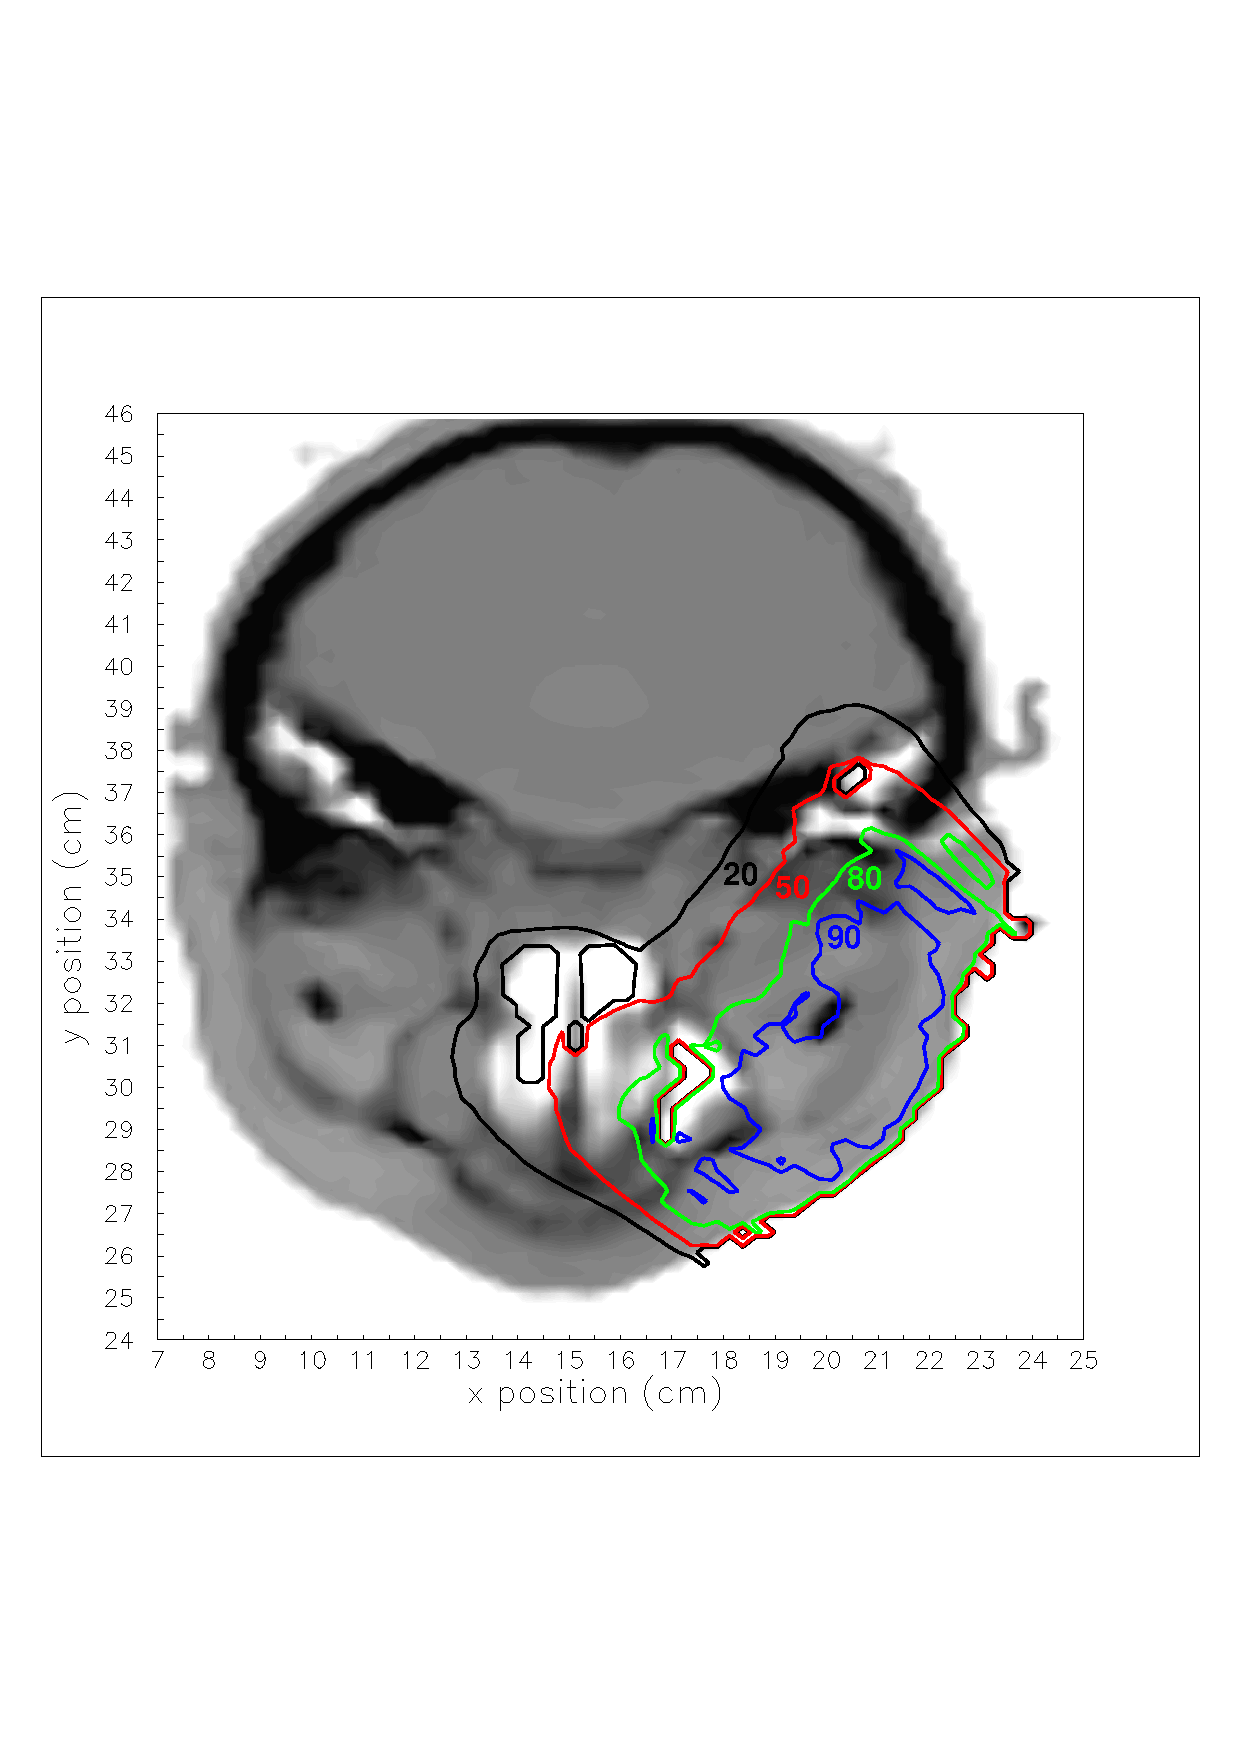
\includegraphics[height=20cm]{figures/CT_example_msmodel}
\end{center}
\end{figure}
\begin{htmlonly}       %%%%%%%%%%%%%%%%%%%%%%%%%%%%%%%%%%%%%%%%%%%%%%
\begin{rawhtml}
</center>
\end{rawhtml}
\end{htmlonly}       %%%%%%%%%%%%%%%%%%%%%%%%%%%%%%%%%%%%%%%%%%%%%%


\vfill
\copyright NRC Canada, 2021
\end{center}

\newpage
\pagestyle{fancy}
\pagenumbering{arabic}
\setcounter{page}{2}

\newpage

\setlength{\parindent}{0em}

\begin{center}
\begin{Large}
{\bf Abstract}
\end{Large}
\end{center}
\indexm{abstract}
DOSXYZnrc is an EGSnrc-based Monte Carlo simulation code for calculating
dose distributions in a rectilinear voxel phantom and is based directly
on the DOSXYZ code developed for the EGS4 code system (see NRC Report
PIRS-509B). DOSXYZnrc is part of the OMEGA-BEAM system of codes developed
at NRC.  Density and material in every voxel may vary.  A variety of beams
may be incident on the phantom, including full phase-space files from
BEAMnrc  and beams characterized using Beam Characterization models. The
companion program {\tt ctcreate} is capable of reading in a CT data set
of Hounsfield numbers and converting it into the information needed by
DOSXYZnrc to simulate transport in a phantom (i.e.  ~the appropriate
material and density are specified in each voxel).  Any of the available
beams can be incident on this CT phantom.  The code includes a resume
option and can be run on parallel computing platforms.  The statistical
analysis is based on a history by history method as opposed to the batch
method used in DOSXYZ.

This user's manual covers general DOSXYZnrc inputs, geometries and outputs.  It
contains information on how to compile and run DOSXYZnrc using the EGSnrcMP
system. It also describes
the use of {\tt ctcreate}.

\begin{latexonly}
\vspace{11.5cm}
\end{latexonly}

\rule{16.3cm}{0.6mm}\\
\begin{small}
The figure on the front page shows a PAW visualisation of the isodose
curves from a DOSXYZ simulation in which a Clinac 2100c 18MeV electron
beam (simulated using a multiple-source model--with 35 million initial
histories) was
incident on the head and neck of a CT phantom.  The visualisation was
implemented by Daryoush Sheikh-Bagheri.

\end{small}

\newpage

\indexm{contents}
\tableofcontents

\newpage

%\pagestyle{myheadings}

\section{Introduction}

\subsection{Overview}
DOSXYZnrc is a general-purpose Monte Carlo EGSnrc\cite{Ka99a,KR00}
\indexm{EGSnrc}
user-code for 3-dimensional absorbed dose calculations. EGSnrc/DOSXYZnrc
simulates the transport of photons and electrons in a Cartesian volume and
scores the energy deposition in the designated voxels. DOSXYZnrc is ``stand
alone'', in the usual EGSnrc sense in that it is controlled by
the {\tt \*.pegs4dat} and {\tt \*.egsinp} files and
is capable of writing out ASCII formatted dose distribution arrays.  The
code uses the EGSnrcMP system which is described in detail in its own
Users Manual\cite{Ka03}.
There is also a graphical user interface (GUI) which allows
input files to be created and executed graphically\cite{TR99}.  Much of the information
in this manual is conveniently accessible via the GUI's help files.


The geometry is a rectilinear volume with
\indexm{geometry coordinate system}
the X-Y plane on the page,  X to the right, Y down the page
and the Z-axis into the page.
Voxel dimensions are completely variable in all three directions. Every
voxel (volume element) can have different materials and/or varying
densities (for use with CT data).  The code allows sources such as a
monoenergetic diverging or parallel beam, phase-space data generated by a
BEAMnrc simulation, or a model-based beam reconstruction produced by BEAMDP.
\indexm{BEAMDP}

DOSXYZnrc has a number of important and unique features such as dose
component calculations, a wide variety of source configurations and beam
reconstruction techniques, CT to phantom conversion
(via {\tt ctcreate}), resume capabilities, phase-space redistribution, \etc.
\indexm{ctcreate}

{\tt ctcreate} is a stand alone program which converts CT data sets into the
data needed for DOSXYZnrc to do a simulation. At present it handles ADAC
Pinnacle, AAPM, CADPLAN and DICOM formats for the CT files.
\indexm{Pinnacle CT}
If you develop extensions, why not
\indexm{CADPLAN CT}
\indexm{DICOM CT}
share them with your colleagues?  Send them to us and we will integrate
them into the standard distribution with full acknowledgement of the
source.

The DOSXYZnrc code, in common with the BEAMnrc system is written for a
preprocessor of Fortran77 called {\tt MORTRAN}. The user does not need
to know {\tt MORTRAN} to use the code, but its elements are needed for
modifications (see refs~\cite{Ne85} or \cite{KR00}).

\subsection{History of DOSXYZnrc}

\indexm{history of DOSXYZnrc}

DOSXYZ started out as a demonstration code that Dave Rogers wrote in March
1986 to show Ralph Nelson that special purpose coding of rectilinear
voxels was faster than using Ralph's more general macros.  At about that time
it was used to estimate the time required to do a full Monte Carlo
treatment planning calculation and the results published 3 years later in
a book chapter\cite{RB90}.  It then became the basis for a Monte Carlo
timing benchmark\cite{BR92} which was regularly updated and available
on the WWW for many years (until 2000).
The OMEGA project took this code over and
added a variety of different source routines with coding contributions
from Charlie Ma, Bruce Faddegon, George Ding, Dave Rogers,  Alex Bielajew,
and Paul Reckwerdt.  More recent modifications have reduced the array
space used by the code, and added beam characterization inputs (Charlie
Ma), btree inputs, (Brian Geiser, but no longer supported), correlated
sampling (Mark Holmes, but no longer supported).
Blake Walters and Mark Holmes added the CT
reading ability in summer 1996.  Blake Walters separated out the
{\tt ctcreate} code in summer 1997 to make the DOSXYZ code much smaller and
thus
able to handle much larger array sizes.  Blake Walters added the
{\tt dsurround} option for reducing simulation time for depth-dose curves
and dose profiles and also the coding for parallel processing in 1998.
\indexm{ctcreate} In 1999, an option was added to allow the user to
run N parallel jobs using a phase space source that exists in N
separate pieces (option now only available using the old
{\tt pprocess} script and not with the new built-in parallel processing
functionality).

Prior to the 1999 revD of this manual, the authors included Paul
Reckwerdt, Mark Holmes and Brian Geiser who had been involved with the
original code to read Pinnacle CT data sets, correlated sampling and
BTREE beam modelling respectively.  These extensions are either no longer
used or are not supported and, thus, these authors are no longer included
as authors of the users manual.  Manuals and/or notes by Geiser and Holmes
are available separately describing BTREE\cite{Ge95} and
correlated sampling\cite{Ho99}.  This latter manual used to be part of
the DOSXYZ Users Manual prior to 1999.

In 2001, with the help of Iwan Kawrakow, Blake Walters ported the
DOSXYZ code to the EGSnrc system to give DOSXYZnrc. At the same time
the statistical analysis routines were converted to a much improved,
history by history approach\cite{Wa02a} instead of the standard batch
approach used in DOSXYZ.

In 2004, Iwan Kawrakow and Blake Walters ported DOSXYZnrc to the new
EGSnrcMP system\cite{Ka03}.  This eliminated the exclusive use of Linux/Unix scripts
and allowed DOSXYZnrc to be compiled and run on Windows-based systems in
addition to Linux/Unix platforms.  At this time, DOSXYZnrc operates
similarly to a standard EGSnrcMP user code, although it is only distributed
as part of the OMEGA/BEAM system.

Although Charlie Ma is no longer an author of the DOSXYZnrc version of the
code, his major contributions to the original EGS4 version still remain.

\vfill

\subsection{Compatibility of DOSXYZ and DOSXYZnrc}

After renaming a DOSXYZ input file from {\tt filename.egs4inp} to {\tt
filename.egsinp}, the file can be used directly by DOSXYZnrc.  This is
because DOSXYZnrc assumes particular default values for all of the
additional EGSnrc input parameters needed.  However, a better approach is
to use the GUI for DOSXYZnrc ({\tt dosxyznrc\_gui}) to read in the DOSXYZ file
and then output the DOSXYZnrc input file with all of the defaults
explicitly stated.  For further information, see
section~\ref{egsnrc_inputs} on page~\pageref{egsnrc_inputs}.

The results of calculations with DOSXYZ and DOSXYZnrc will be very similar
for most situations.  The one systematic difference is that the
relativistic spin corrections to the multiple scattering cause the
depth-dose curves for electron beams to be about 1.5\% more penetrating in
water for a given
electron energy\cite{Wa00}.
\index{DOSXYZ!differences}
\index{DOSXYZ!input file compatibility}
\vfill
\newpage


\section{Compiling/running DOSXYZnrc}
\indexm{compiling!DOSXYZnrc}

\subsection{Files Related to DOSXYZnrc and ctcreate}
\label{filesect}

\indexm{\$HEN\_HOUSE}
As an EGSnrcMP user code, the DOSXYZnrc files are mostly contained in
the directory {\tt \$HEN\_HOUSE/user\_codes/dosxyznrc/},
while {\tt ctcreate} files are
\indexm{ctcreate}
in {\tt \$OMEGA\_HOME/progs/ctcreate/}.  For a general description of the
file structure see Chapter 1 of the BEAMnrc User's Manual \cite{Ro04a}.
\indexm{file structure}

The following describes some files related to DOSXYZnrc:

\begin{description}

\index{dosxyznrc\_gui}
\item[{\tt dosxyznrc\_gui}] This is the Tcl graphical user interface for
creatingi, modifying or executing DOSXYZnrc input files.  Files
related to this are located in
{\tt \$OMEGA\_HOME/progs/gui/dosxyznrc}.  See the GUI manual\cite{TR99}
for more details.
\indexm{graphical user interface}


\item [{\tt egsnrc\_cshrc\_additions} (or {\tt egsnrc\_bashrc\_additions})]
Located in\\ {\tt \$HEN\_HOUSE/scripts}.  If using a Linux/Unix system,
this file must be sourced
in the user's {\tt .cshrc} (or {\tt .bashrc}) file.  It defines useful
aliases for compiling/running DOSXYZnrc.
\indexm{files!egsnrc\_cshrc\_additions}
\indexm{files!egsnrc\_bashrc\_additions}
\indexm{egsnrc\_cshrc\_additions}
\indexm{egsnrc\_bashrc\_additions}

\indexm{Makefile}
\indexm{files!Makefile}
\item [{\tt Makefile}] Located in {\tt \$HEN\_HOUSE/user\_codes/dosxyznrc}.
This file is used by the GNU {\tt make} utility to handle compilation of
\indexm{config.conf}
\indexm{beamnrc.spec}
DOSXYZnrc.  Includes\\ {\tt \$HEN\_HOUSE/specs/config.conf}
(where {\tt config} is the configuration you are using) and
{\tt \$HEN\_HOUSE/specs/beamnrc.spec} files to define environment variables
\indexm{RANDOM}
\indexm{ranmar}
and compiler options.  Also, with the {\tt RANDOM} variable, it defines
the random number generator used (current default is {\tt ranmar}).  Finally,
\indexm{SOURCES}
it defines the variable {\tt SOURCES} which determines the
macros and MORTRAN sources that are
\indexm{mortjob.mortran}
concatenated together to create {\tt mortjob.mortran} (the code that is
actually MORTRAN compiled).
There are two versions of this file, called {\tt Makefile.MS} and  {\tt
Makefile.NOMS}, on the distribution. The default  {\tt Makefile} is  {\tt
Makefile.NOMS} which does not use multiple source models  (source 4, beam
characterization models).  {\tt Makefile.MS} is to be used when Multiple
Source models are to be used (read the file for instructions).
\indexm{beam characterization models}
\indexm{source routines!beam characterization}

\indexm{dosxyznrc.make}
\indexm{files!dosxyznrc.make}
\item[{\tt dosxyznrc.make}] Located in {\tt \$HEN\_HOUSE/user\_codes/dosxyznrc}.  This is an empty file that must exist for compilation using the
{\tt make} utility.

\item[{\tt dosxyznrc.mortran}]  Located in {\tt \$HEN\_HOUSE/user\_codes/dosxyznrc}.  Main {\tt MORTRAN} source code.
\indexm{files!dosxyznrc.mortran}
\indexm{dosxyznrc.mortran}

\item[{\tt srcxyznrc.mortran}]  Located in {\tt \$HEN\_HOUSE/user\_codes/dosxyznrc}.
Subroutines for source configuration inputs + energy spectrum
\indexm{files!srcxyznrc.mortran}
\indexm{srcxyznrc.mortran}

\item[{\tt srcxyznrc.macros}]  Located in {\tt \$HEN\_HOUSE/user\_codes/dosxyznrc}.
{\tt MORTRAN} macros required by {\tt srcxyznrc.mortran}
\indexm{files!srcxyz.macros}
\indexm{srcxyznrc.macros}

\indexm{files!read\_write\_pardose.c}
\indexm{read\_write\_pardose.c}
\indexm{.pardose}
\item[{\tt read\_write\_pardose.c}]  Located in {\tt \$HEN\_HOUSE/user\_codes/dosxyznrc}.  C subroutines used in DOSXYZnrc to
write and read binary {\tt .pardose} output during parallel jobs.  If you
have a C or C++ compiler, then this is compiled when the OMEGA/BEAM
\indexm{read\_write\_pardose.o}
system is installed and {\tt read\_write\_pardose.o} is put
in directory {\tt \$HEN\_HOUSE/lib/config}, where {\tt config} is the
name of your configuration.  If you do not have a C or C++ compiler, then
\indexm{parallel calculations}
this file is not compiled, and the built-in parallel functionality of
DOSXYZnrc cannot be used.

\indexm{files!dosxyznrc\_config.spec}
\indexm{dosxyznrc\_config.spec}
\item[{\tt dosxyznrc\_config.spec}]  (where {\tt config} is the
name of your configuration) Located in\\
{\tt \$HEN\_HOUSE/specs}.  This file is created during OMEGA/BEAM
installation and determines whether or not
the compiled C routines for reading/writing {\tt .pardose} files,
{\tt read\_write\_pardose.o}, are linked in at compile time or not.
If they are to be linked (i.e., you have a C or C++ compiler and
{\tt read\_write\_pardose.c} was compiled successfully), then
\indexm{PARDOSE\_OBJECTS}
the variable {\tt PARDOSE\_OBJECTS} in this file is set
to\\ {\tt \$(EGS\_LIBDIR)read\_write\_pardose.o}, where\\
{\tt \$(EGS\_LIBDIR)}={\tt \$HEN\_HOUSE/lib/config}.  If the
routines are not to be linked at compile time (i.e., you do not
have a C or C++ compiler or {\tt read\_write\_pardose.c} was not
compiled successfully), then {\tt PARDOSE\_OBJECTS} is left blank.

\item[{\tt dosxyznrc\_user\_macros.mortran}] Located in
{\tt \$HEN\_HOUSE/user\_codes/dosxyznrc}.  \\
{\tt MORTRAN} macros that
the user may change  - includes defaults for various options such as beam
models, \etc.  Note that {\tt dosxyznrc\_user\_macros} is also used
by ctcreate to define the maximum dimensions of the DOSXYZnrc phantom
output.
\indexm{files!dosxyznrc\_user\_macros.mortran}
\indexm{dosxyznrc\_user\_macros.mortran}

\item[{\tt dosxyznrc.io}]  Located in {\tt \$HEN\_HOUSE/user\_codes/dosxyznrc}.  This file assigns file names to Fortran unit numbers for output
files not opened explicitly in {\tt dosxyznrc.mortran}.  Currently, the
only files that use this are the {\tt .egslst} file (Fortran unit 1) and
the {\tt .errors} file (Fortran unit 15).
\indexm{files!dosxyznrc.io}
\indexm{dosxyznrc.io}

\indexm{files!phsp\_macros.mortran}
\indexm{phsp\_macros.mortran}
\item[{\tt phsp\_macros.mortran}] {\tt MORTRAN} macros used to read
phase space sources.  This file is always picked up from the
{\tt \$HEN\_HOUSE/utils} directory.

\indexm{files!iaea\_phsp\_macros.mortran}
\indexm{iaea\_phsp\_macros.mortran}
\item[{\tt iaea\_phsp\_macros.mortran}] {\tt MORTRAN} macros used to handle
IAEA-format phase space sources.  Located in the
{\tt \$HEN\_HOUSE/utils} directory, this file is only included if
EGSnrc was installed on a machine with a working C++ compiler and the
library of IAEA phase space handling routines
({\tt \$HEN\_HOUSE/iaea\_phsp/iaea\_phsp.a}) was compiled successfully.
Otherwise, these macros are defined as blank ({\tt \{;\}}) in
{\tt phsp\_macros.mortran} and IAEA functionality does not exist.

\item[{\tt beammodel\_macros.mortran}]    {\tt MORTRAN} macros required
by the multiple-source model for beam reconstruction (source 4), stored in
{\tt \$OMEGA\_HOME/progs/beamdp}.
\indexm{files!beammodel\_macros.mortran}
\indexm{beammodel\_macros.mortran}
\indexm{BEAMDP}

\item[{\tt beammodel\_routines.mortran}]    {\tt MORTRAN} subroutines
required by the multiple-source model for beam reconstruction (source 4),
stored in {\tt \$OMEGA\_HOME/progs/beamdp}.
\indexm{files!beammodel\_routines.mortran}
\indexm{beammodel\_routines.mortran}

\indexm{files!DOSXYZnrc\_examples}
\indexm{DOSXYZnrc\_examples}
\item[{\tt DOSXYZnrc\_examples/}] A subdirectory of
{\tt \$HEN\_HOUSE/user\_codes/dosxyznrc}.  This directory contains sample
input files for DOSXYZnrc.

\end{description}

The following is a description of some of the files related to
{\tt ctcreate}:

\begin{description}

\indexm{files!Makefile}
\indexm{Makefile}
\item[{\tt Makefile}] Located in {\tt \$OMEGA\_HOME/progs/ctcreate}.
Used by the GNU {\tt make} utility, this file
\indexm{SOURCES}
\indexm{mortjob.mortran}
directs the compilation of {\tt ctcreate}.  The {\tt SOURCES} variable defines
the macros and MORTRAN sources concatenated to create {\tt mortjob.mortran}
(which is ultimately MORTRAN compiled)

\item[{\tt ctcreate.mortran}] Located in {\tt \$OMEGA\_HOME/progs/ctcreate}.
This is the main {\tt MORTRAN} source code for
{\tt ctcreate}.
\indexm{files!ctcreate.mortran}
\indexm{ctcreate.mortran}

\indexm{files!ReadCT\_DICOM.c}
\indexm{ReadCT\_DICOM.c}
\indexm{DICOM format}
\item[{\tt ReadCT\_DICOM.c}] Located in {\tt \$OMEGA\_HOME/progs/ctcreate}.
This is a C subroutine for reading CT images in DICOM format.  It is linked
to {\tt ctcreate.mortran} at compile time.

\indexm{files!tags\_ct.h}
\indexm{tags\_ct.h}
\indexm{DICOM format}
\item[{\tt tags\_ct.h}] Located in {\tt \$OMEGA\_HOME/progs/ctcreate}.  This
is a C header file used with {\tt ReadCT\_DICOM.c}.  It defines the
hexadecimal data identifiers used in DICOM image format.

\item[{\tt lnblnk1\_function.mortran}]{\tt MORTRAN} macro to provide the
FORTRAN {\tt lnblnk} function for all configurations.  This is picked
up from {\tt \$HEN\_HOUSE/src}.
\indexm{files!lnblnk1\_function.mortran}
\indexm{lnblnk1\_function.mortran}

\end{description}

\subsection{Compiling and Running DOSXYZnrc}
\label{candrsect}

The commands for compiling and running DOSXYZnrc are
similar to those for other EGSnrcMP user codes
(see the EGSnrcMP Users Manual\cite{Ka03}).
For EGS4 users, please note that file extensions have
changed from, {\em eg,} {\tt file.egs4inp} to {\tt file.egsinp}.
\indexm{.egsinp}
\indexm{.egs4inp}
\indexm{files!.egsinp}
\indexm{files!.egs4inp}

\indexm{DOSXYZnrc!installation}
DOSXYZnrc is normally compiled on your user area as part of the
OMEGA/BEAM user set up
(see the BEAMnrc Manual \cite{Ro04a} for configuration instructions).
To compile DOSXYZnrc independently
(e.g., necessary if you have changed some parameters in \\
{\tt dosxyznrc\_user\_macros.mortran}), ensure that
{\tt Makefile}, {\tt dosxyznrc.make},\\ {\tt dosxyznrc.mortran},
{\tt dosxyznrc\_user\_macros.mortran}, {\tt srcxyznrc.mortran},\\
{\tt srcxyznrc.macros}, and {\tt dosxyznrc.io}
exist in your\\ {\tt \$EGS\_HOME/dosxyznrc} directory (they
should have been copied there automatically from
{\tt \$HEN\_HOUSE/user\_codes/dosxyznrc} during
OMEGA/BEAM configuration).
Then, from {\tt \$EGS\_HOME/dosxyznrc}, compile DOSXYZnrc by typing:
\indexm{make}
\begin{verbatim}
make [options]
\end{verbatim}
The options for {\tt make} are:
\indexm{make!options}
\begin{verbatim}
make              Compile with default optimization
make opt          turned on.  Default optimization is level 2 (-O2).

make noopt        Compile with no optimization

make debug        Compile executable for debugging.

make fortran      Do mortran compilation only, leaving behind the Fortran
                  file dosxyznrc.F.

make clean        Remove the Fortran file, mortjob.mortran file,
                  dosxyznrc.mortlst file and the executable.
\end{verbatim}

\indexm{mf}
\indexm{egsnrc\_cshrc\_additions}
\indexm{egsnrc\_bashrc\_additions}
\indexm{compile\_user\_code}
To preserve compatibility with old usage, the {\tt mf} command is also
available for compiling DOSXYZnrc on a Linux/Unix system (you must have
sourced\\
{\tt \$HEN\_HOUSE/scripts/egsnrc\_cshrc\_additions} or\\
{\tt \$HEN\_HOUSE/scripts/egsnrc\_bashrc\_additions} from your
{\tt .cshrc} or {\tt .bashrc} file).  {\tt mf} is
aliased to the script {\tt \$HEN\_HOUSE/scripts/compile\_user\_code}.

To use {\tt mf}, go into {\tt \$EGS\_HOME/dosxyznrc} and type:
\begin{verbatim}
m[f] dosxyznrc [a] [opt|noopt|debug]
\end{verbatim}
\index{mf!options}
The options for {\tt mf} are:
\verb+mf         =>+ Mortran and Fortran compile and then link\\
\verb+m          =>+ Mortran compile and create the Fortran file\\
\verb+opt        =>+ use optimization (default level 2)\\
\verb+noopt      =>+ use no optimization\\
\verb+debug      =>+ create executable ready for a debug run\\
The parameter ``{\tt a}" is not used and is only present for compatibility
with the previous version of {\tt mf}.

Once you have successfully compiled DOSXYZnrc, the executable,
{\tt dosxyznrc*}, will be left in your {\tt \$EGS\_HOME/bin/config} directory
(where {\tt config} is the name of the configuration that you are using).

\indexm{running DOSXYZnrc}
\indexm{input file}
\indexm{pegs data file}
To run DOSXYZnrc interactively from the command line, go into
{\tt \$EGS\_HOME/dosxyznrc} and type:
\begin{verbatim}
dosxyznrc -i inputfile -p pegsdata
\end{verbatim}
where the input file is {\tt \$EGS\_HOME/dosxyznrc/inputfile.egsinp} and the
file\\
 {\tt pegsdata.pegs4dat} contains the PEGS4 data set (it can be on
{\tt \$EGS\_HOME/pegs4/data} or if not found there, on
{\tt \$HEN\_HOUSE/pegs4/data}).

\index{ex}
If you are using a Unix/Linux system, then you can also start
an interactive DOSXYZnrc run using
the {\tt ex} (aliased to {\tt \$HEN\_HOUSE/scripts/run\_user\_code})
command:
\begin{verbatim}
ex dosxyznrc inputfile pegsdata
\end{verbatim}
{\tt ex} is provided to preserve compatibility with old usage.

\indexm{parallel jobs}
\indexm{batch jobs}
\indexm{running DOSXYZnrc!in batch}
If you are using a Linux/Unix system then you can also run DOSXYZnrc
in batch mode.  Batch submission is required for parallel jobs.
Batch submission uses the {\tt exb} command, which is aliased to
the script {\tt \$HEN\_HOUSE/scripts/run\_user\_code\_batch}.  The syntax
of the {\tt exb} command is:
\begin{verbatim}
exb dosxyznrc inputfile pegsdata [short|medium|long] [batch=batch_sys] [p=N]
\end{verbatim}
\indexm{queues}
\indexm{at} \indexm{NQS} \indexm{PBS} \indexm{keg} \indexm{SGE}
The {\tt [short|medium|long]} option defines the name of the
queue that is used (default is {\tt long} as at NRC).  The {\tt batch\_sys} input
defines the network queuing system to use.  Currently,
{\tt batch\_sys} can be set to {\tt at} (the standard Unix batch
command), {\tt pbs} (to use PBS), {\tt keg} (to use Sun's SGE) or
{\tt nqs} (for NQS).  The default is {\tt at} unless otherwise specified
by setting the environment variable {\tt \$EGS\_BATCH\_SYSTEM}.  Finally,
{\tt N} is used if you are submitting parallel jobs and is set equal to
the number of jobs that you want to split the simulation into.
\indexm{running DOSXYZnrc in parallel}
\indexm{\$EGS\_BATCH\_SYSTEM}

\indexm{temporary working directory}
Once a run is started, a temporary working directory is created as
a subdirectory of\\
{\tt \$EGS\_HOME/dosxyznrc}.  This temporary working directory
has the name\\
{\tt egsrun\_pid\_inputfile\_hostname}, where where {\tt pid} is the process ID number and {\tt hostname} is the name of the
computer the job is running on.  All output files are written
to this temporary directory.  At the end of the run, the files are moved into
{\tt \$EGS\_HOME/dosxyznrc} and the temporary working directory is
deleted.  For more information on temporary working directories, see the
EGSnrcMP Users Manual\cite{Ka03}.

\indexm{.3ddose}
\indexm{files!.3ddose}
\indexm{STATDOSE}
\indexm{output files}
\indexm{.egslst}
\indexm{.pardose}
DOSXYZnrc outputs the following files: {\tt
inputfile.egslst, inputfile.egslog} (for batch runs only, where it
contains screen output), {\tt
inputfile.egsdat} (which can be used to resume the calculation) and {\tt
inputfile.3ddose} which contains a summary of the data in all regions and
can be used by STATDOSE to create {\tt xmgr/xmgrace} graphs (see ``STATDOSE
Users Manual''\cite{MC95} ).  If this is a parallel run, then the
individual jobs will output binary {\tt .pardose} files instead of
{\tt .3ddose} files.  The {\tt .pardose} are then combined automatically at
the end of the parallel run to create a {\tt .3ddose} file.  See section~\ref{parallelcalc} for more information on parallel runs.
Note that the \indexm{inputfile} {\tt
.egslst} file can become VERY long and thereby become useless so use it
carefully for getting the dose which usually can
be more effectively obtained  via the
{\tt .3ddose} output file.
\indexm{xmgrace}
\indexm{xmgr}
\indexm{files!.egslog}
\indexm{.egsinp}
\indexm{files!.egslst}
\indexm{files!.egsdat}
\indexm{.egsdat}
\indexm{.egslog}

\indexm{compiling DOSXYZnrc!from the GUI}
\indexm{running DOSXYZnrc!from the GUI}
\indexm{dosxyznrc\_gui}
The DOSXYZnrc code can also be compiled and run from the
{\tt dosxyznrc\_gui}\cite{TR99}.
To compile DOSXYZnrc, select ``Compile'' from the ``Run'' menu.  This
will open up a window which gives you the different {\tt make} options
(ie optimization vs no optimization, debug, etc).  To run the code
from the GUI, you must first load an existing input file or create a new
one (new inputs or changes to an input file must first be saved before
running).  Then select ``Run'' from the ``Run'' menu.  This will open
up a window in which you can either run DOSXYZnrc interactively
or else submit to a queue (or start a parallel run).  Batch runs will use
the PBS queueing system unless otherwise specified in the
\indexm{\$EGS\_BATCH\_SYSTEM environment\\ variable}
{\tt \$EGS\_BATCH\_SYSTEM} environment variable.  Dialog that would normally
appear on screen during an interactive run now appears in the GUI
run window.

For more information about compiling and running user codes, see the
EGSnrcMP Users Manual\cite{Ka03}.

\subsubsection{Including source 4/beam characterization}

\label{include4}
\indexm{beam characterization models}
\indexm{files!beammodel\_macros.mortran}
\indexm{beammodel\_macros.mortran}
\indexm{files!beammodel\_routines.mortran}
\indexm{beammodel\_routines.mortran}
\indexm{source routines!beam characterization} To implement beam
characterization models in DOSXYZnrc, copy\\ {\tt beammodel\_macros.mortran}
and {\tt beammodel\_routines.mortran}, to the user's {\tt dosxyznrc} area
from {\tt \$OMEGA\_HOME/progs/beamdp}. Also copy {\tt Makefile.MS}
from\\ {\tt \$HEN\_HOUSE/user\_codes/dosxyznrc/} to the user's {\tt
dosxyznrc} area
 and rename it {\tt Makefile}.
Then recompile.
\indexm{BEAMDP}


\subsection{Statistical Analysis}

The statistical analysis in the original DOSXYZ code was done using a standard
batching technique.  Starting with DOSXYZnrc the statistics on the doses are determined by grouping scored quantities
(i.e., energy deposited) on a history-by-history basis
and then determining the uncertainties.
For most sources, this simply means
grouping quantities by incident particle.  However, for phase space sources,
where more than one incident particle may be traced back to a single
primary history, quantities are grouped by primary history.  For more
information, see the published paper on history by history
statistics in DOSXYZnrc and BEAMnrc\cite{Wa02a}.
\indexm{statistics}
\indexm{uncertainties}
\indexm{batch statistics}

It is worth noting that the method used takes into account the latent
variance in any phase space file being used as a source (i.e. the
uncertainty introduced by the statistical variations in the phase space
file). Hence, one cannot reduce the uncertainty in any dose calculation
below that level by recycling the data a large number of times.  However,
one can get an artificially low statistical result which ignores this
latent variance
if the phase space source is allowed to restart the phase space file
instead of using the recycle option (whereby each particle is used multiple
times as it is read in - see section~\ref{nrcycl}, page~\pageref{nrcycl}).
Thus, in order to get accurate uncertainty estimates,
restarting the phase space file should be avoided.
\indexm{NRCYCL}
\indexm{restart phase space}


\section{DOSXYZnrc Input Parameters}
\indexm{input parameters for DOSXYZnrc}

\subsection{Descriptions in DOSXYZnrc Source Code}
\label{DOSXYZ_input}

This section describes input parameters for DOSXYZnrc. The following descriptions
can be found in the beginning of the {\tt dosxyznrc.mortran} source code.
\indexm{graphical user interface}
The graphical user interface facilitates creation of these input files
and contains a great deal of on-line help\cite{TR99}.

\begin{small}
\input{inputs/dosxyznrc.inp}
\end{small}
\clearpage
\section{Source Routines}
\subsection{Source Types in DOSXYZnrc}
\indexm{source routines!summary}
The following source types have been developed for DOSXYZnrc:
\vspace*{-5mm}
\begin{itemize}
\item Parallel rectangular beam incident from the front (isource = 0)
\item Parallel rectangular beam  incident from any direction (isource = 1)
\item Phase-space source, particles incident from any direction
(isource = 2)
\item Point source incident from the front (isource = 3)
\item Beam characterization model, particles incident from any direction
(isource = 4)
\item Uniform isotropically radiating parallelepiped within DOSXYZnrc volume\\
(isource = 6)
\item Parallel rectangular beam incident from multiple angles (isource = 7)
\item Phase-space source incident from multiple angles (isource = 8)
\item Full BEAM treatment head simulation as source (isource = 9)
\item Full BEAM treatment head simulation as source incident from multiple
angles (isource = 10)
\item Phase space source incident
from multiple angles, with multiple SSD's and isocentres--options to run source through a shared library
geometry (defined by BEAM or other MLC code) and synchronize with geometry settings in the case of
a BEAM shared library (isource = 20)
\item BEAM treatment head simulation incident from multiple angles, with multiple SSD's and isocentres--options
to synchronize with BEAM geometry settings and run source through a shared library geometry (other MLC code) (isource = 21)
\end{itemize}
For all sources, the first input record is:\\
{\tt iqin, isource, ......}\\

\clearpage

\subsection{isource = 0: Parallel Rectangular Beam Incident from Front}
\indexm{source routines!isource = 0}
\indexm{source routines!parallel front}

The uniform parallel rectangular beam is always assumed to be incident parallel
to the Z-axis from the front of the phantom. The input parameters are:

\begin{description}
\item [~~~~{\tt iqin}] Charge of the incident beam (-1: electron, 0: photon, 1: positron)
\indexm{iqin}
\item [~~~~{\tt isource}] = 0
\item [~~~~{\tt xinl,xinu}] Lower and upper x-bounds on the phantom surface
\indexm{xinl,xinu}
\item [~~~~{\tt yinl,yinu}] Lower and upper y-bounds on the phantom surface
\indexm{yinl,yinu}
\item [~~~~{\tt thetax}] Angle of the beam relative to the x-axis (degrees)
\indexm{thetax}
\item [~~~~{\tt thetay}] Angle of the beam relative to the y-axis (degrees)
\indexm{thetay}
\item [~~~~{\tt thetaz}] Angle of the beam relative to the z-axis (degrees)
\indexm{thetaz}

\end{description}

\begin{figure}[htbp]
\begin{center}
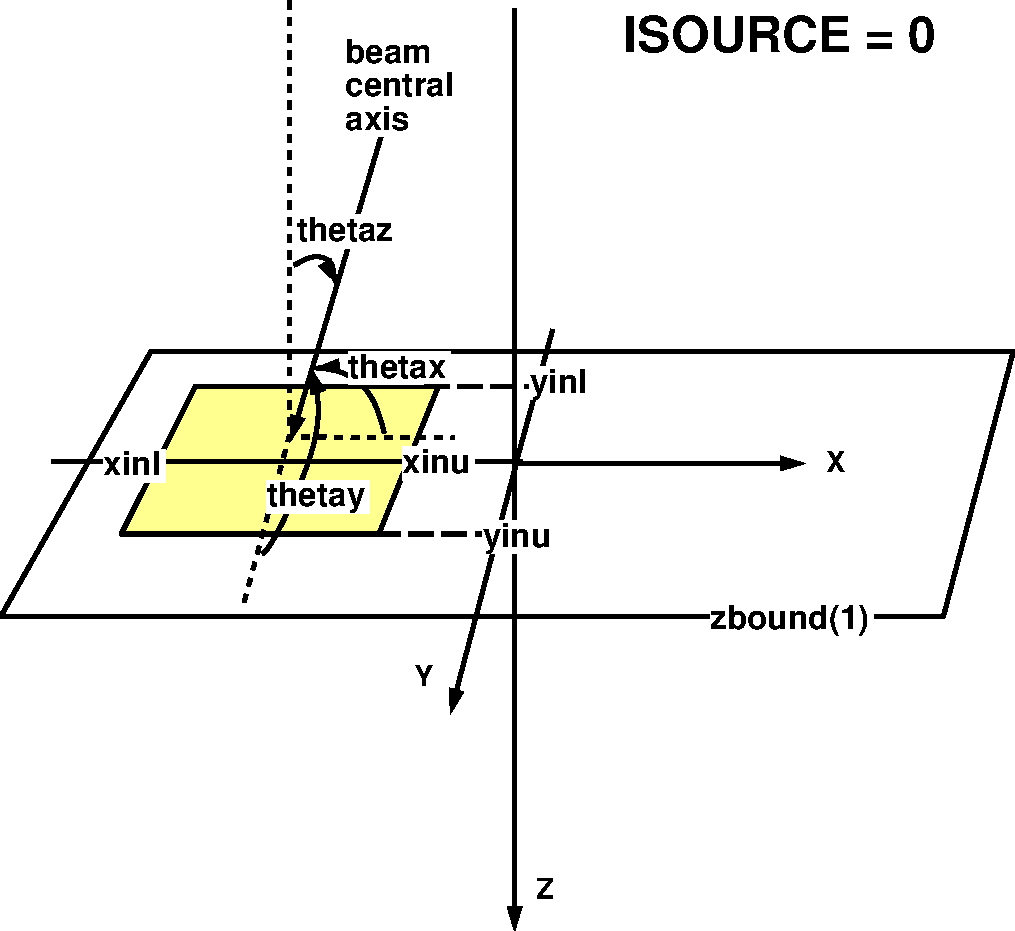
\includegraphics[height=12cm]{figures/src0}
\caption{Parallel rectangular beam (isource=0) showing the beam field, defined by
{\tt xinu}, {\tt xinl, yinu}, and {\tt yinl} on the phantom surface and the
beam directions, {\tt thetax}, {\tt thetay}, and {\tt thetaz}.
The angles {\tt thetax} and {\tt thetay} are relative to the positive x- and y-axes respectively,
while {\tt thetaz} is measured relative to the negative z-axis.}
\label{fig_src0}
\end{center}
\end{figure}
\indexm{xinl,xinu}
\indexm{yinl,yinu}
\indexm{thetax}
\indexm{thetay}
\indexm{thetaz}

\clearpage

\rfoot[]{}

\subsection{isource = 1: Parallel Rectangular Beam Incident from Any Direction}
\indexm{source routines!isource = 1}
\indexm{source routines!parallel any direction}

This uniform parallel rectangular beam may be incident from any direction. The input parameters are:

\begin{description}
\item [~~~~{\tt iqin}] Charge of the incident beam (-1: electron, 0: photon, 1: positron)
\indexm{iqin}
\item [~~~~{\tt isource}] = 1
\item [~~~~{\tt xiso/yiso/ziso}] x-, y-, z-coordinates of the isocenter.  The
isocenter is normally inside the phantom.
\indexm{xiso,yiso,ziso}

\item [~~~~{\tt theta}]   Angle between the +z direction and a line joining
the center of the beam where it strikes the phantom surface to the
isocenter.  In a polar coordinate system, this angle is known as the polar
angle and normally has a range 0-180 degrees.  Note that a centred beam
incident along the +z-axis (ie from the top) has {\tt theta}=180 degrees.
{\tt theta} is
not to be confused with {\tt thetaz} for isource=0, for which case {\tt
thetaz}=0 degrees to aim the source=0 beam along the +z-axis.
\indexm{thetaz}
\indexm{theta}


\item [~~~~{\tt phi}]      Angle  between the +x direction and the
projection on the x-y plane of the line joining the center of the beam on
the phantom surface to the isocenter on the xy plane.  In a polar
coordinate system, this angle is known as the azimuthal angle and normally
has a range 0-360 degrees.
\indexm{phi}

\item [{\tt xcol}/{\tt ycol}]  Total x- and y-widths of the beam on
the plane perpendicular to the beam direction, defined by the center of
the beam and the isocenter
\indexm{ycol}
\indexm{xcol}

\item [{\tt phicol}]  Angle by which the collimator is rotated in the
collimator plane perpendicular to the beam direction.  {\tt phicol} is
determined for {\tt theta}={\tt phi}=0.  The positive sense of rotation is
counterclockwise as one sights down the beam direction.  Note that the
effect of setting {\tt phicol}=90 degrees is the same as switching the
values of {\tt xcol} and {\tt ycol} when {\tt theta} and {\tt phi} are 0
or are both multiples of 90 degrees.
\indexm{theta}
\indexm{phicol}
\end{description}

\clearpage

\rfoot[{\sffamily \rightmark}]{{\sffamily \leftmark}}

\begin{figure}[htbp]
\begin{center}
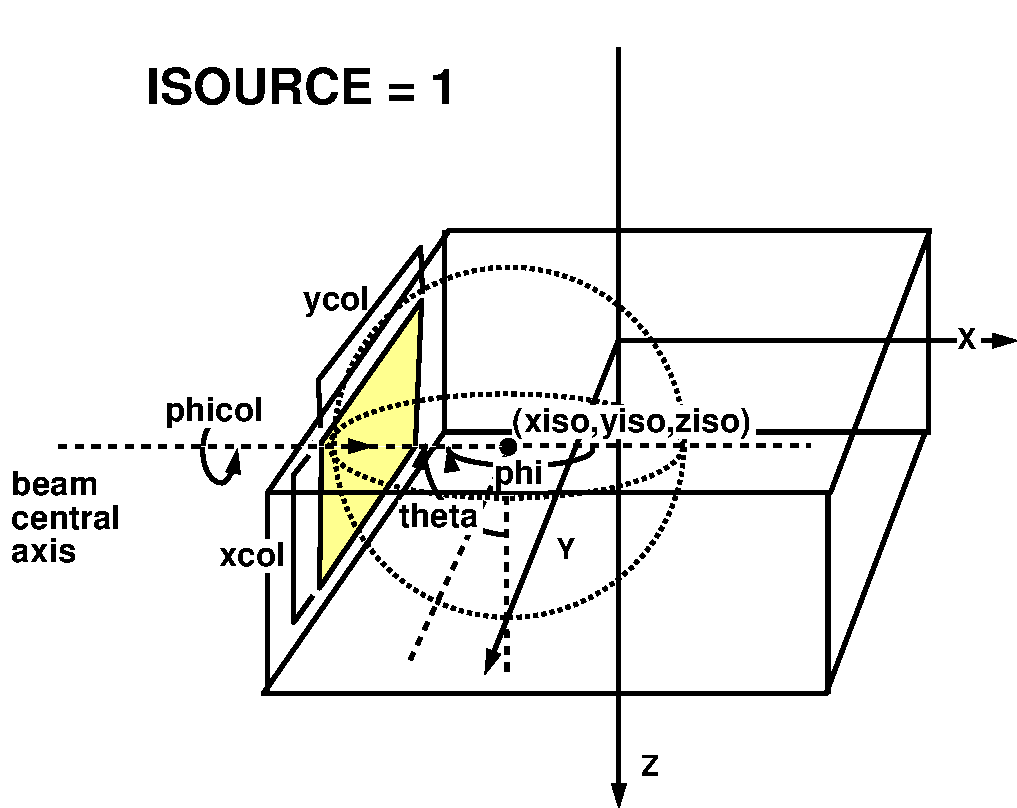
\includegraphics[width=16cm]{figures/src1}
\caption{Parallel rectangular beam incident from any direction (isource=1).  A
polar coordinate system is set up at the isocenter, (xiso,yiso,ziso).  The
position of the beam collimator is then defined using the angles, {\tt
theta} and {\tt phi}.  In the particular example shown in this figure,
with the beam incident on the centre of the negative Y face of the volume,
{\tt theta} is 90 degrees and {\tt phi} is 180 degrees.  The dimensions of
the rectangular collimator are given by {\tt xcol} and {\tt ycol}.  An
additional degree of freedom is available by allowing the collimator to
rotate in its own plane by angle {\tt phicol}.  Note that source 1 is
always incident right on the phantom surface (ie particles do not travel
through air to get to the phantom)}
\label{fig_src1}
\end{center}
\end{figure}
\indexm{xiso,yiso,ziso}
\indexm{theta}
\indexm{phi}
\indexm{phicol}

\clearpage

\subsection{isource = 2: Phase-Space Source Incident from Any Direction}
\label{source2sect}
\indexm{source routines!isource = 2}
\indexm{source routines!phase space}

This source uses a phase-space file generated during a BEAMnrc simulation at
any flat scoring plane of a linear accelerator geometry. A user can choose
any particular type of particles from the phase-space file and score dose
components using the {\tt LATCH} filter. The field size of the incident
\indexm{LATCH} beam can be reduced using the parameter {\tt BEAM\_SIZE}.
There is also a
\indexm{BEAM\_SIZE} parameter called {\tt ISMOOTH} which
can be set to 1 if one wants to shift
\indexm{ISMOOTH} the particles to
their symmetrical positions with respect to x- and y-axis in the
phase-space file for repeated use of these phase-space particles. For {\tt
ISMOOTH} = 0, no shift will be made when phase-space particles are
re-used.  {\tt LATCH} filter, {\tt BEAM\_SIZE} and {\tt ISMOOTH} are input
later in the file.
\indexm{re-use of phase space}

Input parameters for a phase-space source are:
\begin{description}
\item [~~~~{\tt iqin}] Charge of the incident beam (-1: electron, 0:
\indexm{iqin}
            photon, 1: positron, 2: all particle types)
\item [~~~~{\tt isource}] = 2
\item [~~~~{\tt xiso/yiso/ziso}] x-, y-, z-coordinates of the isocenter
\indexm{xiso,yiso,ziso}
                 (normally located within the phantom)
\item [~~~~{\tt theta}]   Same as for isource=1.
\indexm{theta}

\item [~~~~{\tt phi}]     Same as for isource=1.
\indexm{phi}
\item [~~~~{\tt dsource}]      For a BEAMnrc format phase space source, this
is the absolute distance from the isocenter to the
source center, which is, by definition, the origin of the phase-space
plane (origin may not even be in the beam).  For an IAEA format phase
space source, this is the distance from the isocentre to the primary
source ({\it i.e.} the source used to generate the phase space file), or
SAD.
\indexm{dsource}

\item [~~~~{\tt phicol}]  Angle by which the source is rotated in the
                     source plane perpendicular to the beam direction.
                     {\tt phicol} is determined for {\tt theta}={\tt phi}=0.
                     The positive sense of rotation is counterclockwise
                     as one sights down the beam direction.
\indexm{phicol}

\indexm{DBS}
\indexm{directional bremsstrahlung splitting}
\item [~~~~{\tt i\_dbs}] Set to 1 if the phase space source was generated
using directional bremsstrahlung splitting (DBS) in BEAM {\bf AND} you
wish to reject photons directed outside the splitting field (which will
all be fat).  Set to 0 otherwise.  Note that {\tt i\_dbs} is read in as
a real and converted to integer.
\indexm{i\_dbs}

\item [~~~~{\tt r\_dbs}] Radius (in cm) of the DBS splitting field in
the BEAMnrc simulation used to generate this source. Only needed if {\tt
i\_dbs} = 1.
\indexm{r\_dbs}

\item [~~~~{\tt ssd\_dbs}] SSD (in cm) where the DBS splitting field radius
was defined in the BEAMnrc simulation used to generate this source.
Only needed if {\tt i\_dbs} = 1.
\indexm{ssd\_dbs}

\item [~~~~{\tt z\_dbs}] Z value (in cm) in the BEAMnrc simulation
where this phase space source was scored.  This will be at the back of
a component module (CM).  Only needed if {\tt i\_dbs} = 1.
\indexm{{\tt z\_dbs} }

\item [~~~~{\tt e\_split}]  Number of times to split charged particles
as soon as they enter the phantom geometry.  Split particles have their
weight reduced by a factor of 1/{\tt e\_split}.  This is only used
in conjunction with photon splitting ({\tt n\_split}, see Section~\ref{nsplitsect}) and
prevents higher-weight contaminant electrons from compromising statistics
in photon beams.  For maximum efficiency, it is suggested that you
set {\tt e\_split}={\tt n\_split}, the photon splitting number.
\indexm{source 2!charged particle splitting}
\indexm{e\_split}

\indexm{{\tt FILNAM}}
\item [~~~~{\tt FILNAM}] The full name (including extension) of the phase space file
(including the directory path).  In the case of an IAEA-format phase space
source, the full name of the phase space data ({\tt .IAEAphsp}) file
\indexm{IAEA phase space source}
is input here.  The header ({\tt .IAEAheader}) file as assumed to exist
in the same directory.  For more information about IAEA-format date, see
the BEAMnrc Manual.

\end{description}

{\tt theta}, {\tt phi} and {\tt dsource} can be set to place the source
anywhere inside the phantom or the surrounding region; the medium and the
thickness of the surrounding region is input by the user.  Particles from
the phase space which are initially outside both the phantom and surrounding
region are terminated immediately.  If the medium of the surrounding
region is air, for example,  the phase-space particles will be transported
{\it properly} through air to the surface of the phantom. A particle
history is terminated if it is determined that the particle will not make
it to the phantom surface (the particle loses all its energy in the
surrounding region or it escapes through the outer boundaries of the
surrounding region).


Note that, for source 2, the user must set {\tt enflag} = 2 or 3, input
the \indexm{enflag}
mode of the phase-space file (0 or 2), and input the medium number and the
thickness for the surrounding region.  The user should also input the
phase-space file name after the above inputs.  These other inputs are
described in sections 5 and 6 below.  For more information related to
phase-space sources, see the section on phase-space files in the
BEAMnrc User's Manual
\cite{Ro04a}.

The value of {\tt phicol} must be set to 180 degrees in order for the X-Y
coordinates in a BEAMnrc-generated phase space source to map onto the
equivalent X-Y coordinates in DOSXYZnrc.  This is because of the general
coordinate transformation done going from BEAMnrc to DOSXYZnrc.

\subsubsection[DBS Inputs]{Inputs related to directional bremsstrahlung
splitting}
\label{i_dbs_sect}

\indexm{DBS}
\indexm{directional bremsstrahlung splitting}
\indexm{fat photons}
If you have used the directional bremsstrahlung splitting (DBS) variance
reduction technique (see the BEAMnrc User's Manual\cite{Ro04a} for more
details) to
generate the phase space source, then it is recommended that you use
the inputs {\tt i\_dbs}, {\tt r\_dbs}, {\tt ssd\_dbs} and {\tt z\_dbs} to
prevent unsplit, high-weight (``fat") photons which are outside the
splitting field from compromising your dose statistics.
{\tt r\_dbs} and {\tt ssd\_dbs} (the DBS splitting field radius and
SSD in cm) are available directly from the inputs for DBS in the BEAM
simulation, while {\tt z\_dbs} is simply the Z value at the back of the
component module (CM) in the BEAMnrc simulation in which this phase space source was scored.  If
{\tt i\_dbs} is set to 1, then before a photon is used in the DOSXYZnrc
simulation, it is projected along its trajectory from {\tt z\_dbs}
to {\tt ssd\_dbs} (we assume {\tt ssd\_dbs}$\geq${\tt z\_dbs}).  If it
falls outside {\tt r\_dbs} at {\tt ssd\_dbs}, then the photon is
not used in the DOSXYZnrc simulation.  In the context of the BEAM simulation
this photon will not have been split and will be fat (but this information
is not carried in the phase space file except indirectly because of the
larger weight which is not a unique specifier).  To be able to ignore these
fat photons and thereby increase the efficiency considerably, it is
important to ensure that the dose from the photons being ignored is
negligible. This can usually be arranged by making the splitting field big
enough.
\indexm{DBS}
\indexm{directional bremsstrahlung splitting}

Note that charged particles are not
rejected with this technique, which means that if you do not want fat charged
particles to compromise dose statistics (especially near the surface of a
phantom) then you must use the electron splitting option in DBS
(again, see the BEAMnrc User's Manual for more details).

\subsubsection{IAEA format phase space sources}
\label{src2iaeasect}
\indexm{source 2!IAEA format phase space file}
In the case of an IAEA format phase space source, the input, {\tt dsource} (see above), defines the distance
from the primary source ({\it i.e.} the source used to generate the phase space file) to the phantom
isocentre, or SAD.  This is because, unlike BEAMnrc format phase space files, the incident Z-position of
particles is available and read from either the phase space data (in the case of 3-D phase space files) or the header file
(in the case of planar phase space files, such as those scored by BEAMnrc).  The input value of {\tt dsource} is then
subtracted from this Z-position to give the distance along the beam axis from the phantom isocentre to the
particle incident position.

The ability of source 2 to automatically handle IAEA phase space files in which the Z-position for each
particle is scored (3-D data) is particularly useful in cases where the phase space data available for
an accelerator is scored on a non-planar surface (as is the case with the data that Varian has made
available for their TrueBeam accelerators) or when using 3-D phase space data scored by an upstream
DOSXYZnrc simulation (see Section~\ref{phspoutsect}).

\begin{figure}[htbp]
\begin{center}
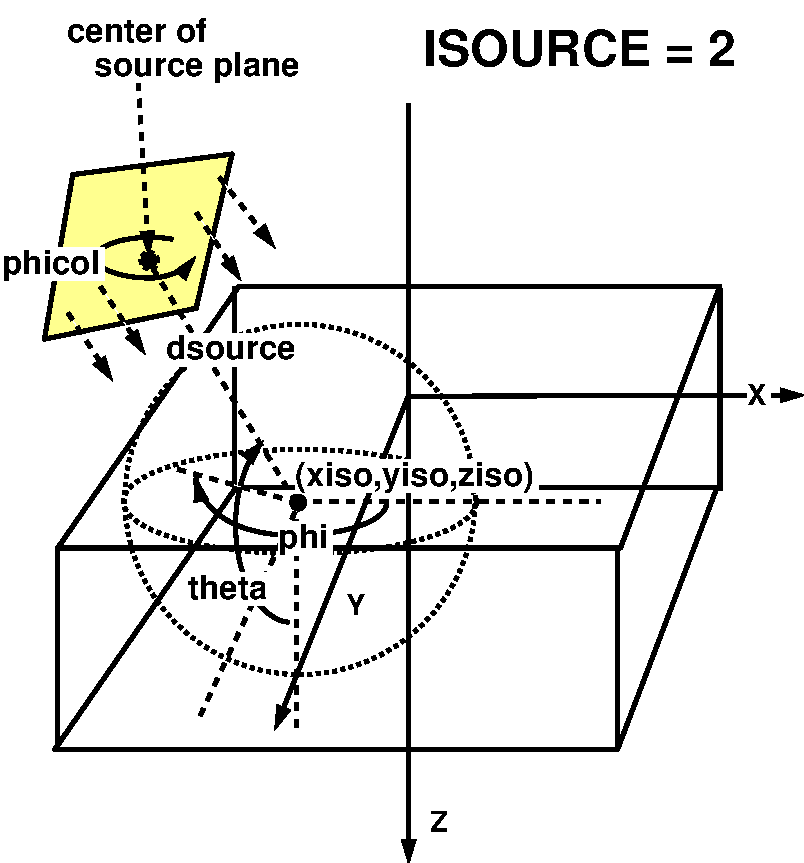
\includegraphics[width=14cm]{figures/src2}
\caption{Phase-space source incident from any direction (isource=2).
Similar to
source 1, a polar coordinate system is set up at the isocenter, (xiso,
yiso, ziso).  The position of the origin in the phase-space plane is then
defined by the angles {\tt theta} and {\tt phi}, and the distance from the
isocenter, {\tt dsource}.  The source can be rotated in its own plane
using the variable {\tt phicol}.  The figure shows that the source plane
does not necessarily have to be right against the surface of the phantom,
however it must be within the surrounding region specified by {\tt dsurround}
 (see section ~\ref{sec5}).}
\label{fig_src2}
\end{center}
\end{figure}
\indexm{dsource}
\indexm{phicol}
\indexm{theta}
\indexm{phi}
\indexm{xiso,yiso,ziso}
\indexm{dsurround}

\clearpage

\subsection{isource = 3: Point Source Rectangular Beam Incident from Front}
\indexm{source routines!isource = 3}
\indexm{source routines!point source rectangle}

The isotropically-radiating point source is placed on the Z-axis.  It is
assumed to be incident on the front surface of the phantom, but can be
placed any distance above the phantom.  The beam field can be asymmetric.

The input parameters for the point source are:
\begin{description}

\item [~~~~{\tt iqin}] Charge of the incident beam (-1: electron, 0:
\indexm{iqin}
                  photon, 1: positron)
\item [~~~~{\tt isource}] = 3
\item [~~~~{\tt xinl,xinu}] Lower and upper x-bounds of the field on the
\indexm{xinl,xinu}
          phantom surface
\item [~~~~{\tt yinl,yinu}] Lower and upper y-bounds of the field on the
\indexm{yinl,yinu}
                   phantom surface
\item [~~~~{\tt ssd}] Distance from the point source to the phantom surface (cm)
\indexm{ssd}
\end{description}

Note that, between the source and the phantom surface the medium is
assumed to be a vacuum for this source.

\begin{figure}[htbp]
\begin{center}
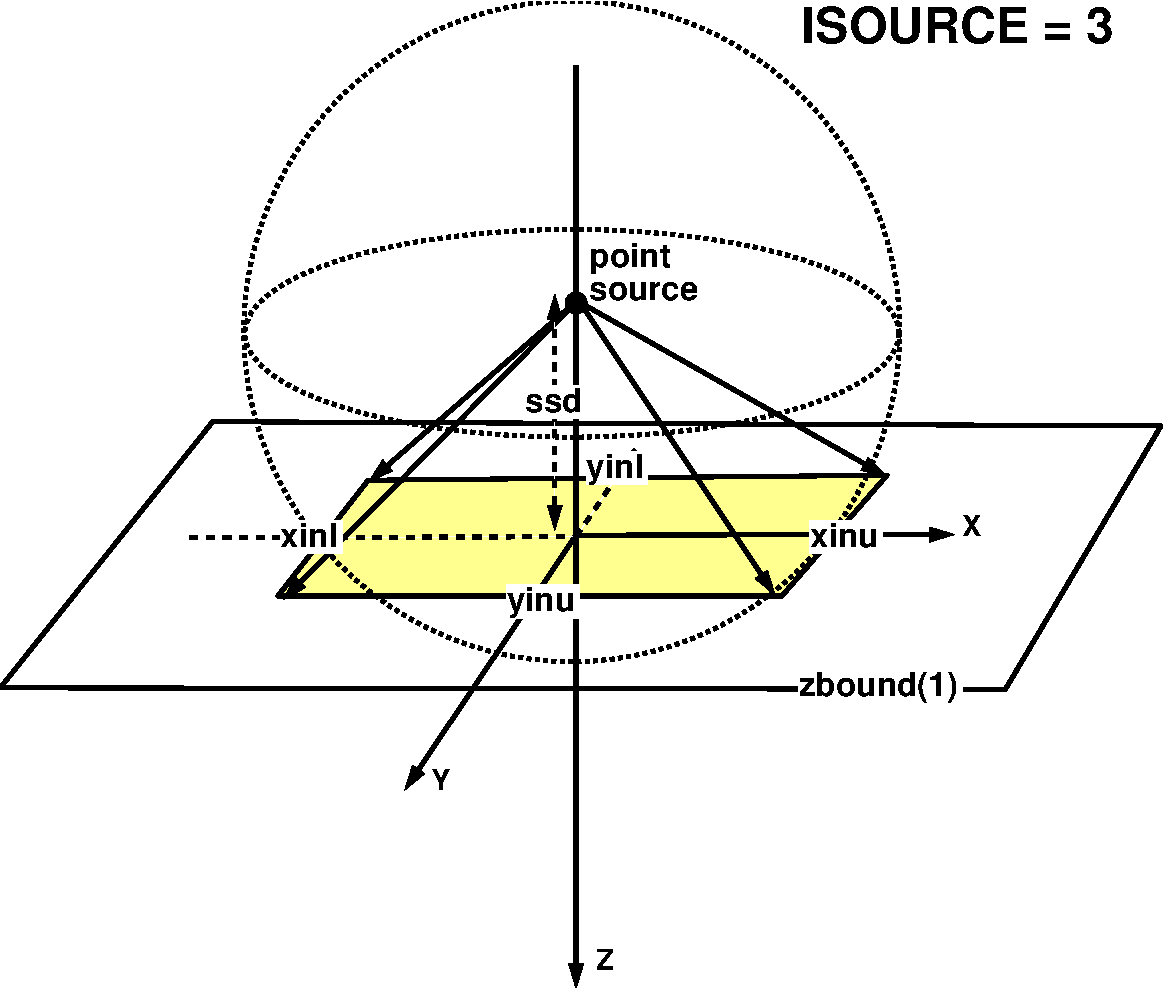
\includegraphics[height=11cm]{figures/src3}
\caption{Point source incident from the front (isource=3).  The
isotropically-radiating point source is located on the Z-axis at distance
ssd above the phantom.  The source is collimated to a rectangular field
defined by xinu, xinl, yinu, yinl on the phantom surface.}
\label{fig_src3}
\end{center}
\end{figure}
\indexm{xinl,xinu}
\indexm{yinl,yinu}

\clearpage


\subsection{isource = 4: Beam Characterization Model Incident
from Any Direction}
\indexm{source routines!isource = 4}
\indexm{source routines!beam characterization}

This source uses the beam characterization models created by BEAMDP from
phase space
data generated by BEAMnrc. This source consists of a variety of sub-sources
for different types of particles coming from different components of a
linear accelerator. Each sub-source has its own spectral and (planar)
fluence distributions and the correlation between the energy, position and
incident angle is retained by sampling the particle positions on the
sub-source (the surface of the component) and on the phase-place plane. A
beam model input file, generated by BEAMDP, is required by this source.
For more details about beam characterization models see the
BEAMnrc User's Manual and associated paper\cite{Ma95c,Ma97}.
\indexm{BEAMDP}

Apart from {\tt isource}, which must be set to 4, input parameters for source 4 are the same as for source 2:

\indexm{enflag}
Note this source requires {\tt enflag} = 4 and to input the beam model
input file name after the {\tt enflag} input. The field size of the
incident beam can be reduced using the parameter {\tt BEAM\_SIZE}.  These
inputs are described in sections 5 and 6 below.
\indexm{BEAM\_SIZE}

The default version of DOSXYZnrc does not include this source. In order to
use it you must recompile DOSXYZnrc using the instructions in
section~\ref{include4}. .

\clearpage

\rfoot[]{}

\subsection{isource = 6: Uniform Isotropically Radiating Parallelepiped
within DOSXYZnrc Volume}
\indexm{source routines!isource = 6}
\indexm{source routines!beam characterization}

This source allows the user to simulate a uniform isotropically radiating
rectangular volume (parallelepiped) within the DOSXYZnrc phantom.
The active volume is restricted to being completely contained within the
DOSXYZnrc phantom.  However, it can be shrunk to a point anywhere within the
phantom.

The input parameters for the uniform isotropically radiating parallelepiped:
\begin{description}

\item [~~~~{\tt iqin}] Charge of the incident beam (-1: electron, 0:
\indexm{iqin}
                  photon, 1: positron)
\item [~~~~{\tt isource}] = 6
\item [~~~~{\tt xinl,xinu}] Lower and upper x-bounds of the active volume (cm)
\indexm{xinl,xinu}
\item [~~~~{\tt yinl,yinu}] Lower and upper y-bounds of the active volume (cm)
\indexm{yinl,yinu}
\item [~~~~{\tt zinl,zinu}] Lower and upper z-bounds of the active volume (cm)
\indexm{zinl,zinu}
\end{description}

\begin{figure}[htbp]
\begin{center}
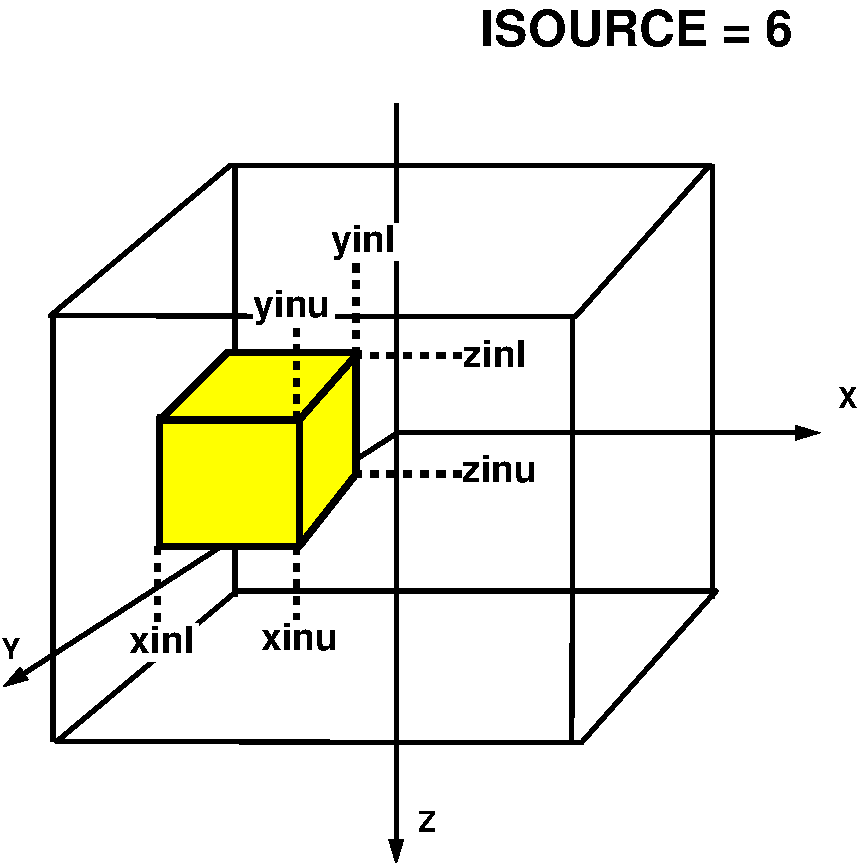
\includegraphics[height=11cm]{figures/src6}
\caption{Uniform isotropically radiating parallelepiped within DOSXYZnrc phantom
(isource=6).  The active volume, specified by {\tt xinl, xinu, yinl,
yinu, zinl, zinu}, must fit within the phantom.  The source can be shrunk
to a point within the phantom by setting {\tt xinu=xinl}, {\tt yinl=yinu}
and {\tt zinl=zinu}.}
\label{fig_src6}
\end{center}
\end{figure}
\indexm{xinl,xinu}
\indexm{yinl,yinu}
\indexm{zinl,zinu}

\clearpage

\subsection{isource = 7: Parallel Rectangular Beam Incident from Multiple Directions}
\label{source7_sec}
\indexm{source routines!isource = 7}
\indexm{source routines!parallel multiple directions}

This is a uniform parallel rectangular beam similar to source 1,
but incident from multiple, user-defined
directions (theta-phi pairs). The input parameters are:

\begin{description}
\item [~~~~{\tt iqin}] Charge of the incident beam (-1: electron, 0: photon, 1: positron)
\indexm{iqin}
\item [~~~~{\tt isource}] = 7
\item [~~~~{\tt xiso/yiso/ziso}] x-, y-, z-coordinates of the isocenter.  The
isocenter is normally inside the phantom.
\indexm{xiso,yiso,ziso}

\item [~~~~{\tt nang}]  The number of incident theta-phi pairs
or, if negative, then abs({\tt nang}) is the number of groups of
incident theta-phi pairs, where, within a group, all theta-phi pairs have
equal probability.  The incident angles theta and phi are defined the
same as they are in source 1.  Theta-phi pairs/groups are specified on
separate lines (see below).
\indexm{nang}
\indexm{theta-phi pairs}

\item [~~~~{\tt xcol}/{\tt ycol}]  Total x- and y-widths of the beam on
the plane perpendicular to the beam direction, defined by the center of
the beam and the isocenter
\indexm{ycol}
\indexm{xcol}

\item [~~~~{\tt phicol}]  Angle by which the collimator is rotated in the
collimator plane perpendicular to the beam direction.  {\tt phicol} is
defined the same way as in source 1.
\indexm{phicol}
\end{description}

And then, on the subsequent {\tt abs(nang)}  lines:\\

{\bf If {\tt nang} $>$ 0:}\\
~~~\\
For i=1,{\tt nang}: {\tt theta(i), phi(i), pang(i)}
\begin{description}
\item [~~~~{\tt theta(i)}]  Theta for pair i (degrees).
\item [~~~~{\tt phi(i)}]  Phi for pair i (degrees).
\item [~~~~{\tt pang(i)}] Probability of particle being incident at
                          Theta(i)-Phi(i).
\indexm{theta(i)}
\indexm{phi(i)}
\indexm{pang(i)}
\end{description}
{\bf If {\tt nang} $<$ 0:}\\
~~~\\
For i=1,-{\tt nang}: {\tt ivary(i), angfixed(i), angmin(i), angmax(i),
ngang(i), pgang(i)}
\begin{description}
\item [~~~~{\tt ivary(i)}] Set to 0 to vary phi in group i; Set to 1 to vary
theta in group i.
\item [~~~~{\tt angfixed(i)}] Fixed theta ({\tt ivary(i)}=0) or phi
({\tt ivary(i)}=1) in group i (degrees).
\item [~~~~{\tt angmin(i)}] Minimum varying phi ({\tt ivary(i)}=0) or
theta ({\tt ivary(i)}=1) in group i (degrees).
\item [~~~~{\tt angmax(i)}] Maximum varying phi ({\tt ivary(i)}=0) or
theta ({\tt ivary(i)}=1) in group i (degrees).
\item [~~~~{\tt ngang(i)}] Number of equally-spaced phi ({\tt ivary(i)}=0) or
theta ({\tt ivary(i)}=1) between and including {\tt angmin(i)} and
{\tt angmax(i)} in group i (Note that, since it includes
{\tt angmin(i)} and {\tt angmax(i)}, {\tt nang(i)} must be $\geq$ 2).
\item [~~~~{\tt pgang(i)}] Probability of particle being in group i.  Within
a group, all theta-phi pairs have equal probability.
\indexm{ivary(i)}
\indexm{angfixed(i)}
\indexm{angmin(i)}
\indexm{angmax(i)}
\indexm{ngang(i)}
\indexm{pgang(i)}
\end{description}

Note that the {\tt pang(i)} are automatically normalized.


\subsection{isource = 8: Phase-Space Source Incident from Multiple Directions}
\label{src8sect}
\indexm{source routines!isource = 8}
\indexm{source routines!phase space from multiple\\ directions}

This source is similar to source 2, except that it is incident from
multiple, user-defined directions (theta-phi pairs).

Input parameters for source 8 are:
\begin{description}
\item [~~~~{\tt iqin}] Charge of the incident beam (-1: electron, 0:
\indexm{iqin}
            photon, 1: positron, 2: all particle types)
\item [~~~~{\tt isource}] = 8
\item [~~~~{\tt xiso/yiso/ziso}] x-, y-, z-coordinates of the isocenter
\indexm{xiso,yiso,ziso}
                 (normally located within the phantom)

\item [~~~~{\tt nang}]  The number of incident theta-phi pairs
or, if negative, then abs({\tt nang}) is the number of groups of
incident theta-phi pairs, where, within a group, all theta-phi pairs have
equal probability.  The incident angles theta and phi are defined the
same as they are in source 2.  Theta-phi pairs/groups are specified the
same way as they are in source 7 (see section~\ref{source7_sec} above).
\indexm{nang}
\indexm{theta-phi pairs}

\item [~~~~{\tt dsource}]      For BEAMnrc phase space files, this
is the absolute distance from the isocenter to the
source center, which is, by definition, the origin of the phase-space
plane (origin may not even be in the beam).  For IAEA phase space files, this
is the primary source to isocentre distance (SAD).
\indexm{dsource}

\item [~~~~{\tt phicol}]  Angle by which the source is rotated in the
                     source plane perpendicular to the beam direction.
                     {\tt phicol} is determined for {\tt theta}={\tt phi}=0.
                     The positive sense of rotation is counterclockwise
                     as one sights down the beam direction.
\indexm{phicol}
\indexm{DBS}
\indexm{directional bremsstrahlung splitting}
\item [~~~~{\tt i\_dbs}] Set to 1 if the phase space source was generated
                     using directional bremsstrahlung splitting (DBS) in
                     BEAMnrc {\bf AND} you wish to reject photons directed outside
                     the splitting field (which will all be fat).  Set to 0 otherwise.
		Note that {\tt i\_dbs} is read in as a real and converted to integer.
\indexm{i\_dbs}
\item [~~~~{\tt r\_dbs}] Radius (in cm) of the DBS splitting field in
the BEAMnrc simulation used to generate this source. Only needed if {\tt
i\_dbs} = 1.  \indexm{r\_dbs}

\item [~~~~{\tt ssd\_dbs}] SSD (in cm) where the DBS splitting field
radius was defined in the BEAMnrc simulation used to generate this
source. Only needed if {\tt i\_dbs} = 1.  \indexm{ssd\_dbs}

\item [~~~~{\tt z\_dbs}] Z value (in cm) in the BEAMnrc simulation
where this phase space source was scored.  This will be at the back of
a component module (CM). Only needed if {\tt i\_dbs} = 1.  \indexm{{\tt
z\_dbs} }

\indexm{e\_split}
\indexm{source 8!charged particle splitting}
\item [~~~~{\tt e\_split}] Number of times to split charged particles
as soon as they enter the phantom.  The weight of split particles
is reduced by a factor of 1/{\tt e\_split}.  This is used in
conjunction with photon splitting (input variable {\tt n\_split}, see
Section~\ref{nsplitsect}) to prevent higher-weight contaminant electrons
from compromising dose statistics.  For optimum efficiency,
set {\tt e\_split}={\tt n\_split}.

\indexm{{\tt FILNAM}}
\item [~~~~{\tt FILNAM}] The full name (including extension) of the phase space
file
(including the directory path).  See the description of
source 2 (Section~\ref{source2sect}) for more details.
\end{description}
An example may help illustrate this input.  The following input:
\typeout{}
\typeout{*******Example end of 4.9 has two extra variables??  *************}
\typeout{*******Example end of 4.9 has two extra variables??  *************}
\typeout{*******Example end of 4.9 has two extra variables??  *************}
\typeout{}
\begin{verbatim}
0, 8, 0.0, 0.0, 0.0, -1.0, 80.0, 90.0, 0.0, 0.0, 0, 0.0, 0.0, 0.0
1, 90.0, 0.0, 356.40, 100, 1.0
\end{verbatim}
is for source 8. The phase space file rotates about the isocenter at
(0,0,0). The centre of the phase-space is 80 cm from the isocenter and the
collimator angle is 90 degrees.
The -1.0 indicates there is only one group of angles. The 1 at the start of
the second line tells us that phi is fixed (at 90 degrees)
and that theta is varying, in
this case in 100 discrete steps between 0 and 356.4 degrees with equal
intensity at each angle.  In this example, {\tt i\_dbs} is set to 0, indicating
that either directional bremsstrahlung splitting (DBS) was not used in the
BEAMnrc simulation that generated this source or else the user does not wish
to reject high-weight (``fat") photons created by DBS.

For more information on how to use the inputs {\tt i\_dbs},
{\tt r\_dbs}, {\tt ssd\_dbs} and {\tt z\_dbs} see section~\ref{source2sect}
on source 2 above.

Similar to source 2, source 8 automatically handles IAEA format phase space sources
with Z-position scored for each particle (3-D phase space).

\subsection{isource = 9: BEAM Treatment Head Simulation Incident from Any
Direction}
\label{src9sect}
\indexm{source routines!isource = 9}
\indexm{source routines!full BEAM simulation}

This source uses particles sampled from a BEAM simulation running
concurrently with the DOSXYZ
\indexm{BEAM accelerator code}
simulation.  The BEAM accelerator code must be compiled as a shared
library (existing in directory {\tt \$EGS\_HOME/bin/config}, where
{\tt config} is the name of your configuration) and must be supplied
with its own input file and pegs data file.  More details about this
are given below.  Source particles for DOSXYZ are then sampled from what
would be the scoring plane during a normal run of the BEAM accelerator.
Thus, this source is similar to {\tt isource}=2 (full phase space file)
without the need to store a phase space file.

\indexm{C/C++ compiler}
\indexm{config.conf file}
\indexm{BEAMLIB\_OBJECTS}
\indexm{BEAMLIB\_EXTRA\_LIBS}
Note that if you are running on Unix/Linux you must have a working C/C++
compiler to use this source and the file
{\tt \$HEN\_HOUSE/specs/config.conf} ({\it i.e.} file {\tt \$EGS\_CONFIG})
must have the variable
{\tt BEAMLIB\_OBJECTS} set to
\indexm{load\_beamlib.o}
{\tt \$(HEN\_HOUSE)lib/\$(my\_machine)/load\_beamlib.o} and\\
{\tt BEAMLIB\_EXTRA\_LIBS} set to {\tt $-$ldl}.
If you have installed EGSnrcMP on a Unix/Linux system with a working C/C++
compiler, the installation will automatically compile the C code
\indexm{load\_beamlib.c}
{\tt \$HEN\_HOUSE/cutils/load\_beamlib.c} to create
{\tt load\_beamlib.o}, and {\tt BEAMLIB\_OBJECTS} and
{\tt BEAMLIB\_EXTRA\_LIBS} will
automatically be set to their proper values.  Otherwise
{\tt BEAMLIB\_OBJECTS} and
{\tt BEAMLIB\_EXTRA\_LIBS} will remain
undefined (ie definitions left blank).

If you are running on Windows, then there is no requirement to have
a working C/C++ compiler to use this source.  In this case, the installation
automatically sets {\tt BEAMLIB\_OBJECTS} in
{\tt \$HEN\_HOUSE/specs/config.conf} to
\indexm{load\_beamlib.obj}
{\tt \$(HEN\_HOUSE)lib/\$(my\_machine)/load\_beamlib.obj}, where
{\tt load\_beamlib.obj} is a precompiled version of {\tt load\_beamlib.o}
included with the installation.  {\tt BEAMLIB\_EXTRA\_LIBS} does not
need to be defined and is left
blank.  See the BEAMnrc Manual\cite{Ro04a} for more information about
{\tt config.conf} files.

Similar to {\tt isource = 2}, you can select particles from the BEAM simulation
\indexm{LATCH}
to use based on their charge and/or {\tt LATCH} values.   You can also
select the maximum size of the BEAM field considered using the
\indexm{BEAM\_SIZE}
{\tt BEAM\_SIZE} input (discussed in more detail in its own section below).

Input parameters for source 9 are:
\begin{description}
\item [~~~~{\tt iqin}] Charge of the incident beam (-1: electron, 0:
\indexm{iqin}
            photon, 1: positron, 2: all particle types)
\item [~~~~{\tt isource}] = 9
\item [~~~~{\tt xiso/yiso/ziso}] x-, y-, z-coordinates of the isocenter
\indexm{xiso,yiso,ziso}
                 (normally located within the phantom)
\item [~~~~{\tt theta}]   Same as for isource=2.  Recall that, for a
beam coming down from the top of the phantom, {\tt theta}=180 degrees.
\indexm{theta}

\item [~~~~{\tt phi}]     Same as for isource=2.
\indexm{phi}
\item [~~~~{\tt dsource}]      Absolute distance from the isocenter to the
centre of the source plane, which is, by definition, the origin of the
scoring plane in the BEAM simulation.
\indexm{dsource}

\item [~~~~{\tt phicol}]  Angle by which the source is rotated about the
                     BEAM central axis.
                     {\tt phicol} is determined for {\tt theta}={\tt phi}=0.
                     The positive sense of rotation is counterclockwise
                     for {\tt theta}=0.  If {\tt theta}=180 degrees
                     (ie beam coming down from the top), then
                     {\tt phicol} must be set to 180 degrees to have the
                     BEAM x-y coordinates match the DOSXYZ x-y coordinates.
\indexm{phicol}

\indexm{DBS}
\indexm{directional bremsstrahlung splitting}
\item [~~~~{\tt i\_dbs}] Set to 1 if directional bremsstrahlung splitting
(DBS) is being used in the BEAM simulation {\bf AND} you wish to reject
fat photons falling outside the DBS splitting field.  This is recommended
so that the fat photons do not compromise dose statistics.  Note that,
with {\tt isource}=9, we have direct access to the BEAM stack variable
({\tt IPHAT}) indicating whether a photon is fat or not, thus we do not
need to reconstruct the DBS splitting field using the additional
inputs {\tt r\_dbs}, {\tt ssd\_dbs} and {\tt z\_dbs} required in
source 2.
\indexm{i\_dbs}

\item [~~~~{\tt e\_split}]  Number of times to split charged particles
as soon as they enter the phantom geometry.  Split particles have their
weight reduced by a factor of 1/{\tt e\_split}.  This is only used
in conjunction with photon splitting ({\tt n\_split}, see Section~\ref{nsplitsect}) and
prevents higher-weight contaminant electrons from compromising statistics
in photon beams.  For maximum efficiency, it is suggested that you
set {\tt e\_split}={\tt n\_split}, the photon splitting number.
\indexm{source 9!charged particle splitting}
\indexm{e\_split}

In addition to the above inputs, the user must input the following
information, all on one line, separated by commas. This line of input
follows the {\tt enflag} input line, {\it i.e.} the second line after the
above input.

\indexm{the\_beam\_code}
\item [~~~~{\tt the\_beam\_code}]  The name of the BEAM accelerator
simulation (ie {\tt BEAM\_accelname}).  This code must have been compiled as
a shared library that exists in your\\ {\tt \$EGS\_HOME/bin/config}
directory.  More information
on compiling a BEAM code as a library is given below.

\indexm{the\_input\_file}
\item [~~~~{\tt the\_input\_file}]  The input file to use for the BEAM
simulation (no {\tt .egsinp} extension).  This file must exist in
your {\tt \$EGS\_HOME/BEAM\_accelname} directory (ie the accelerator
directory).  In the BEAM input file, you must define a single scoring plane
in the accelerator, where
the source particles will be sampled, and the BEAM input
parameter {\tt IO\_OPT} must be set to output a phase space file at
this scoring plane.  See the BEAMnrc Manual\cite{Ro04a} for more information
about scoring planes and {\tt IO\_OPT}.  {\tt the\_input\_file} will
define a value of {\tt NCASE} (no. of histories) for the BEAM simulation,
but this is ignored and the BEAM simulation will always run until
{\tt NCASE} for the DOSXYZ simulation is reached.
\indexm{IO\_OPT}
\indexm{NCASE}

\item [~~~~{\tt the\_pegs\_file}]  The pegs data to be used in the BEAM
\indexm{the\_pegs\_file}
simulation (no {\tt .pegs4dat} extension).  This file must exist in
either {\tt \$HEN\_HOUSE/pegs4/data} or
your\\ {\tt \$EGS\_HOME/pegs4/data} directory.

\end{description}

A graphical representation of source 9 is similar to that of
source 2 shown in Figure~\ref{fig_src2}.  In both sources, the
``source plane'' is the scoring plane in the BEAM simulation, but in source 9
particles are sampled as soon as they cross the scoring plane rather than
stored in a phase space file for later use.  Note that the BEAM central
axis points from the origin of the source plane to the isocenter.

Similar to source 2, {\tt theta}, {\tt phi} and {\tt dsource}
can be set to place the source
plane anywhere inside the phantom or the surrounding region; the medium and the
thickness of the surrounding region are input by the user.  Particles
initially falling outside both the phantom and surrounding
region are terminated immediately. A particle history is terminated if it
is determined that the particle will not make
it to the phantom surface (the particle loses all its energy in the
surrounding region or it escapes through the outer boundaries of the
surrounding region).

The user must also set {\tt enflag} = 2 or 3
the \indexm{enflag}
and input the medium number and the
thickness for the surrounding region.
These inputs are described in sections 5 and 6 below.

\subsubsection[Compiling a BEAM library]{Compiling a BEAM code as
a shared library}
\label{make_library_sect}
\indexm{BEAM shared library}

In order to compile your BEAM accelerator code, {\tt BEAM\_accelname}, as
a shared library, you must already have built the code and created your
\indexm{beam\_build}
directory {\tt \$EGS\_HOME/BEAM\_accelname} using the {\tt beam\_build}
tool.  Building a BEAM code is discussed in detail in the BEAM Manual\cite{Ro04a}.
Of course, if you have already been running {\tt BEAM\_accelname} as a
regular BEAM simulation, then the code will have already been built and
{\tt \$EGS\_HOME/BEAM\_accelname} will exist.  To compile the code as a
shared library, go into your directory \\{\tt \$EGS\_HOME/BEAM\_accelname}
and type:
\indexm{make!BEAM shared library}
\begin{verbatim}
make library
\end{verbatim}
\indexm{BEAM shared library!naming scheme}
If you are using a Unix/Linux system, this will create the
library {\tt libBEAM\_accelname.so}.  On a Windows system, the
library will be named {\tt BEAM\_accelname.dll}.  The library will
automatically be copied to your directory {\tt \$EGS\_HOME/bin/config},
where {\tt config} is the name of your configuration
(e.g. {\tt gcc}, {\tt win2k}, {\tt pgf77}, etc).  See the BEAM Manual for the
differences between the codes concatenated to create a BEAM library and those
used for a standard BEAM accelerator simulation.

\indexm{{\tt libg2c.a}}
In previous versions of BEAMnrc, the library {\tt libg2c.a} was required
when compiling shared library sources on Unix/Linux to avoid confusion of
Fortran units between DOSXYZnrc (the driving code) and BEAMnrc.  Recently,
however, the opening of files in BEAMnrc has been recoded so that only
available Fortran units are used.  This solves the problem of confusion
between Fortran units and eliminates the need for the {\tt libg2c.a}
\indexm{{\tt gfortran}}
library (which caused problems with the {\tt gfortran} compiler).

\indexm{the\_beam\_code}
Recall that when entering the input parameter {\tt the\_beam\_code},
specifying the BEAM simulation to use, you
simply use {\tt BEAM\_accelname}, omitting
the {\tt lib} prefix (in the case of a Unix/Linux library) and
the {\tt .so} or {\tt .dll} extension of the library.

\subsubsection[Efficiency of BEAMnrc simulation source vs. phase space source]
{Efficiency of BEAMnrc simulation source vs. a phase space source}
\indexm{BEAMnrc simulation source!efficiency vs. phase space source}

A BEAMnrc source has the obvious advantage over a phase space source
in that intermediate phase space data need not be stored.  For many
calculations with reasonable precision, this can save tens of
GBytes of disk storage space.  In general, the tradeoff will be a
reduced simulation efficiency, due to the extra
time required to perform a full accelerator simulation to generate
source particles.

Recent research\cite{KW06} has shown, however, that
by using variance reduction techniques in the BEAMnrc simulation
source and in the DOSXYZnrc calculation, the efficiencies of photon
beam dose calculations using BEAMnrc simulation sources can be maximized
so that they are only 3--13\% (depending on beam energy, field size and
phantom voxel size) lower than the peak efficiencies with the equivalent
phase space sources.  The variance reduction techniques required are
directional bremsstrahlung splitting (DBS--see Ref\cite{Ka04a}
and Section 6.3.4 in the BEAMnrc Manual) to maximize the efficiency
of photon production in the BEAMnrc simulation source in conjunction
with
photon splitting ({\tt n\_split}--see Section~\ref{nsplitsect}) to
maximize the efficiency of the DOSXYZnrc calculation.  Efficiencies
quoted for phase space sources include the time required to transport
particles through the accelerator jaws (from ``fixed'' phase space data
collected above the jaws) to generate the source, but even if this
time is omitted, the peak efficiencies with BEAMnrc simulation sources
are only 5--30\% lower than those with phase space sources.

\subsection{isource = 10: Full BEAMnrc Treatment Head Simulation Incident from Multiple Directions}
\indexm{source routines!isource = 10}
\indexm{source routines!BEAMnrc simulation source from\\ multiple directions}

This source is similar to source 9, except that it is incident from
multiple, user-defined directions (theta-phi pairs).

Inputs for source 10 are:
\begin{description}
\item [~~~~{\tt iqin}] Charge of the incident beam (-1: electron, 0:
\indexm{iqin}
            photon, 1: positron, 2: all particle types)
\item [~~~~{\tt isource}] = 10
\item [~~~~{\tt xiso/yiso/ziso}] x-, y-, z-coordinates of the isocenter
\indexm{xiso,yiso,ziso}
                 (normally located within the phantom)

\item [~~~~{\tt nang}]  The number of incident theta-phi pairs
or, if negative, then abs({\tt nang}) is the number of groups of
incident theta-phi pairs, where, within a group, all theta-phi pairs have
equal probability.   Same as for source 8 (see Section~\ref{src8sect} above
for more details).
\indexm{nang}
\indexm{theta-phi pairs}

\item [~~~~{\tt dsource}] Absolute distance from the isocenter to the
centre of the source plane.  Same as for source 9 (Section~\ref{src9sect}).
\indexm{dsource}

\item [~~~~{\tt phicol}] Angle by which the source is rotated about the
                     BEAM central axis.  Same as for source 9 (Section~\ref{src9sect}).
\indexm{phicol}

\indexm{DBS}
\indexm{directional bremsstrahlung splitting}
\item [~~~~{\tt i\_dbs}] Set to 1 if directional bremsstrahlung splitting
(DBS) is being used in the BEAM simulation {\bf AND} you wish to reject
fat photons falling outside the DBS splitting field so that they do not
compromise dose statistics.  Same as for source 9 (Section~\ref{src9sect}).
\indexm{i\_dbs}

\item [~~~~{\tt e\_split}]  Number of times to split charged particles
as soon as they enter the phantom geometry.  This is only used
in conjunction with photon splitting ({\tt n\_split}$>$1).
Same as for source 9 (Section~\ref{src9sect}).
\indexm{source 10!charged particle splitting}
\indexm{e\_split}

\indexm{the\_beam\_code}
\item [~~~~{\tt the\_beam\_code}]  The name of the BEAM accelerator
simulation (ie {\tt BEAM\_accelname}).  Same as for source 9 (Section~\ref{src9sect}).

\indexm{the\_input\_file}
\item [~~~~{\tt the\_input\_file}]  The input file to use for the BEAM
simulation (no {\tt .egsinp} extension).  Same as for source 9.

\item [~~~~{\tt the\_pegs\_file}]  The pegs data to be used in the BEAM
\indexm{the\_pegs\_file}
simulation (no {\tt .pegs4dat} extension).  Same as for source 9.

\end{description}

For an example of how the theta-phi pairs are specified, see the
description at the bottom of Section~\ref{src8sect} above.

Note that, similar to source 9, the user must also set {\tt enflag} = 2 or 3 \indexm{enflag} and input the medium number
and the thickness for the surrounding region. These inputs are described in sections 5 and 6 below.

\subsection{isource = 20: Synchronized phase space source}
\label{src20sect}
\indexm{source routines!isource = 20}
\indexm{source routines!Simulation through moving MLC}
\indexm{source routines!synchronized phase space source}

This source greatly enhances the capabilities of the phase space source incident from multiple directions (isource=8).
Source 20 was developed by Lobo and Popescu\cite{LP10} to allow the user to simulate continuous motion of the phase space
source relative to the DOSXYZnrc phantom over specified ranges of incident
directions, SSD's and isocentre coordinates.  Moreover, the source allows
the user to interpose a geometry, generated using either a BEAM accelerator or a non-EGSnrc code (likely simulating
an MLC geometry) compiled as a shared library, between the source plane and the DOSXYZnrc phantom.  In the case of a BEAM shared library, the source
parameters (range of incident directions, SSD's, isocentres) can be synchronized with the field settings of any synchronized
component modules (see the BEAMnrc Manual\cite{Ro09}).

The geometrical parameters controlling the orientation of the source plane relative to the DOSXYZnrc phantom
have the same definition as those for sources 2, 8, 9 and 10 and are shown in Figure~\ref{fig_src2}.

Input parameters for source 20 are:

\begin{description}
\item [~~~~{\tt iqin}]
\indexm{iqin}
Charge of the incident beam (-1: electron, 0: photon, 1: positron, 2: all particle types)
\item [~~~~{\tt isource}] = 20
\item [~~~~{\tt nset}]
\indexm{nset}
\indexm{\$MXANG}
The number of control points.  Control points define the beginning and end points of ranges of incident direction angles, SSD's and isocentre coordinates over which continuous motion of the source is simulated
(see below).  {\tt nset} must be in the range 2 $\leq$ {\tt nset} $\leq$ {\tt \$MXANG}, where {\tt \$MXANG} is defined in
the file\\ {\tt \$EGS\_HOME/dosxyznrc/dosxyznrc\_user\_macros.mortran}.
\item [~~~~{\tt i\_dbs}]
\indexm{i\_dbs}
Set to 1 if the phase space source was generated using directional bremsstrahlung splitting (DBS) in BEAM and you wish
to reject photons directed outside the splitting field (which will all be fat). Set to 0 otherwise. Note that
{\tt i\_dbs} is read in as a real and converted to integer.
\item [~~~~{\tt r\_dbs}]
\indexm{r\_dbs}
Radius (in cm) of the DBS splitting field in the BEAM simulation used to generate this source. Only needed if {\tt i\_dbs}=1.
\item [~~~~{\tt  ssd\_dbs}]
\indexm{ssd\_dbs}
SSD (in cm) where the DBS splitting field radius was defined in the BEAM simulation used to generate this source. Only needed if
{\tt i\_dbs} = 1.
\item [~~~~{\tt z\_dbs}]
\indexm{z\_dbs}
Z value (in cm) in the BEAM simulation where this phase space source was scored. This will be at the back of a component module (CM). Only needed if {\tt i\_dbs} = 1.
\item [~~~~{\tt e\_split}]
\indexm{e\_split}
Number of times to split charged particles as soon as they enter the phantom geometry. Split particles have their weight reduced by a factor of 1/{\tt e\_split}. This is only used in conjunction with photon splitting ({\tt n\_split}, see Section 8.16) and prevents higher-weight contaminant electrons from compromising statistics in photon beams. For maximum efficiency, it is suggested that you set {\tt e\_split=n\_split}, the photon splitting number.
\item [~~~~{\tt i\_muidx\_out}]
\indexm{i\_muidx\_out}
Set to 1 to include the fractional monitor unit index, {\tt MU}, associated with each particle in IAEA format phase
space output for particles leaving the phantom geometry.  Note that phase space data is not output at all
unless
\indexm{i\_phsp\_out}
{\tt i\_phsp\_out}, the input parameter in the main code controlling phase space output, is set to 1 or 2.
If {\tt MU} is included in the phase space output, then phase space data has a time dimension and is considered 4-D.
Scoring of {\tt MU} allows synchronization between the DOSXYZnrc simulation generating the file and any
downstream simulations--such as BEAMnrc simulations with synchronized component modules--using the file as
a source. See Section~\ref{phspoutsect} for a description of DOSXYZnrc phase space output.
\item [~~~~{\tt calflag}]
\indexm{calflag}
\indexm{NRCYCL}
Set to 1 to skip the calibration run through a BEAM shared library geometry between the source plane and
the phantom. The number of times to recycle each source particle before proceeding to the next one,
{\tt NRCYCL}, will then not take into account the ratio of the number of particles emerging from the
library geometry to the number of incident particles (survival ratio).  The default is to do the calibration run if a BEAM shared library geometry is present.
\end{description}

For i=2,...,{\tt nset} (the no. of control points), the following parameters are entered:
\begin{description}
\item[~~~~{\tt xiso(i)/yiso(i)/ziso(i)}]
\indexm{xiso,yiso,ziso}
x-, y-, z-coordinates of the isocenter.
\item[~~~~{\tt theta(i)}]
\indexm{theta(i)}
Angle of line connecting phase space plane to isocentre relative to the +Z axis.
\item[~~~~{\tt phi(i)}]
\indexm{phi(i)}
Angle of line connecting phase space plane to isocentre relative to the +X axis.
\item[~~~~{\tt phicol(i)}]
\indexm{phicol(i)}
2D Angle of rotation of the phase space plane about its own origin.
\item[~~~~{\tt dsource(i)}]
\indexm{dsource(i)}
The distance from the centre of the phase space plane to the isocentre except when an IAEA format phase space source
is used, in which case input the distance from the primary BEAM source to the isocentre (SAD).  When an IAEA phase space
source is used, the distance from the phase space plane to the isocentre is calculated using the Z position of
the phase space plane read in from the IAEA header file.
\item[~~~~{\tt muIndex(i)}]
\indexm{muIndex(i)}
A monitor unit index in the range $[$0,1$]$ defining the fraction of the total number of incident particles
delivered up to control point i.
Note that {\tt muIndex(i)} $\geq$ {\tt muIndex(i-1)}. Also note that for correct selection of the range
of incident source parameters, {\tt muIndex(i)=0.0} and {\tt muIndex(nset)=1.0}.  See below for more information
on how {\tt muIndex} is used to sample from a range of incident source parameters.
\end{description}
End of inputs required for each control point.

\begin{description}
\item[~~~~{\tt the\_shared\_lib}]
\indexm{the\_shared\_lib}
The name of the BEAM accelerator code or non-EGSnrc MLC simulation code compiled as a
shared library (See below for more information).  Leave this blank if there is no geometry interposed between the
phase space source and the DOSXYZnrc phantom.  This code must have been compiled as a shared library
({\it e.g.} {\tt libBEAM\_accelname.so} if a BEAM accelerator compiled on Unix/Linux) and exist in directory
{\tt \$EGS\_HOME/bin/config}, where {\tt config} is your configuration name.
\item[~~~~{\tt FILNAM}]
\indexm{FILNAM}
The full name (including directory path and file extension) of the phase space source.
\item[~~~~{\tt the\_input\_file}]
\indexm{the\_input\_file}
Input file for the BEAM or non-EGSnrc code defining the shared library geometry interposed between the
phase space source and the DOSXYZnrc phantom.  For a BEAM shared library, this input file must exist in
{\tt \$EGS\_HOME/BEAM\_accelname}   In the case of a BEAM shared library, this file must specify phase space
output at the bottom of the accelerator.
\end{description}

\indexm{MU\_RND}
\indexm{Source 20!Example control point settings}
Prior to each incident particle (Note: not necessarily a statistically-independent primary history)
a random number, {\tt MU\_RND}$\in[$0,1$]$, which can be thought of as a fractional monitor unit, is compared to the {\tt muIndex(i)} of the control points
to determine the incident geometrical parameters.  If source 20 is being run through a BEAM shared library geometry which has
synchronized component modules, such as SYNCJAWS and/or SYNCVMLC (See the BEAMnrc Users Manual\cite{Ro09}), then
the value of {\tt MU\_RND} is passed to BEAM from DOSXYZnrc (more on this below).
If {\tt muIndex(i-1)}$\leq${\tt MU\_RND}$<${\tt muIndex(i)}
then the parameters determining the orientation of the source plane are interpolated
between control points i-1 and i using:

\begin{equation}
{\tt PARAM}={\tt PARAM(i-1)}+\frac{\left[{\tt PARAM(i)}-{\tt PARAM(i-1)}\right]}
{\left[{\tt muIndex(i)}-{\tt muIndex(i-1)}\right]}\left[{\tt MU\_RND}-{\tt muIndex(i-1)}\right]
\end{equation}

Where {\tt PARAM} is the value of the source parameter ({\tt xiso}, {\tt yiso}, {\tt ziso}, {\tt theta}, {\tt phi}, etc) used in the simulation, and {\tt PARAM(i)} and {\tt PARAM(i-1)} are its values defined at control points i and i-1, respectively.
Thus, source parameters are evenly distributed between control points i-1 and i.

The generation of a new value of {\tt MU\_RND} for each incident particle means that particles in the phase space source arising
from the same primary history will be incident from different source orientations.  This was implemented to ensure adequate sampling
of source positions even in cases where where relatively few primary histories are represented in the phase space source
({\it i.e.} if the BEAM simulation used to generate the source used directional bremsstrahlung splitting with a high
splitting number).  Note, however, that regardless of how spatially well-sampled a dose distribution is, its uncertainty is
limited by the number of primary histories simulated.

An simple example input segment for {\tt nset}=7 is:

\begin{verbatim}
0, 0, -9, 90, 0, 0, 15, 0
0, 0, -9, 90, 360, 0, 15, 0.1
0, 0, -5, 90, 0, 45, 15, 0.1
0, 0, -5, 90, 360, 45, 15, 0.5
0, 0, 5, 90, 0, 90, 15, 0.5
0, 0, 5, 90, 360, 90, 15, 0.9
0, 0, 9, 90, 360, 135, 15, 1.0
\end{verbatim}

This sample input defines
four distinct ranges of incident source parameters:

\begin{enumerate}
\item The first two control points ({\tt muIndex(1)}=0.0, {\tt muIndex(2)}=0.1) define 10\% of incident particles
with ({\tt xiso, yiso, ziso})=(0, 0, -9), {\tt theta}=90$^o$ (i.e. incident
from the side of the phantom), {\tt phi} evenly distributed over $[$0,360$^o]$ (i.e. circling the entire phantom in the X-Y plane), {\tt phicol}=0$^o$, and {\tt dsource}=15 cm.
\item Control points 3 and 4, with {\tt muIndex(3)}=0.1 and {\tt muIndex(4)}=0.5, define 40\% of incident particles with
({\tt xiso, yiso, ziso})=(0, 0, -5), {\tt theta}=90$^o$, {\tt phi} evenly distributed over $[$0,360$^o]$, {\tt phicol}=45$^o$, and {\tt dsource}=15 cm.  Note that setting {\tt muIndex(3)} = {\tt muIndex(2)} is used to define a discontinuity between
this range and the previous range, since no parameters will be chosen between control points 2 and 3.
\item Control points 5 and 6, with {\tt muIndex(5)}=0.5 and {\tt muIndex(6)}=0.9, define another range of parameters
(discontinuous with the previous one), in which 40\% of incident particles have
({\tt xiso, yiso, ziso})=(0, 0, 5), {\tt theta}=90$^o$, {\tt phi} evenly distributed over $[$0,360$^o]$, {\tt phicol}=90$^o$, and
{\tt dsource}=15 cm.
\item Control point 7 ({\tt muIndex(7)}=1.0) defines 10\% of particles ({\tt muIndex(7)}-{\tt muIndex(6)}=0.1) with
({\tt xiso, yiso, ziso}) evenly distributed over $[$(0, 0, 5),(0, 0, 9)$]$, {\tt theta}=90$^o$, {\tt phi} evenly distributed over $[$0,360$^o]$, {\tt phicol} evenly distributed over $[$90$^o$,135$^o]$ and {\tt dsource}=15 cm.  Note that this range is
continuous with the previous one.
\end{enumerate}

A realistic simulation of a treatment plan may involve hundreds, or thousands, of control points.  In practice these could
either be extracted from a treatment plan or generated using your own code\cite{LP10}.  Note that a large number of
control points may require you to increase the value of {\tt \$MXANG} in {\tt \$EGS\_HOME/dosxyznrc/dosxyznrc\_user\_macros.mortran} (which defines the maximum value of {\tt nset}) and recompile DOSXYZnrc. \indexm{\$MXANG}

\indexm{i\_dbs}
\indexm{z\_dbs}
\indexm{ssd\_dbs}
\indexm{r\_dbs}
It is recommended that the user set the input {\tt i\_dbs}=1 if directional bremsstrahlung splitting (DBS) was used
to generate the phase space source and they wish to eliminate fat photons, directed outside the splitting field, from
the DOSXYZnrc simulation.  From the BEAM simulation used to generate the phase space source, the user must then input
the DBS splitting radius, {\tt r\_dbs}, the Z-position of the scoring plane, {\tt z\_dbs}, and the SSD used for
DBS, {\tt ssd\_dbs}.  See Section~\ref{i_dbs_sect} for more details.

Just as with other phase space sources (sources 2, 8), source 20 requires setting the input parameter, {\tt enflag}, to 2 or 3
(with or without {\tt LATCH} bit filtering), that the mode of the phase space file (0--no {\tt zlast} scoring, 2--{\tt zlast} scoring) be
input, and that the thickness and medium of the region surrounding the phantom be specified.  See Section~\ref{sec5} for more information.

\index{source 20!incident through a shared library geometry}
\subsubsection{Phase space source incident through a shared library geometry}

\indexm{the\_shared\_lib}\indexm{the\_input\_file}
Using the inputs, {\tt the\_shared\_lib} and {\tt the\_input\_file}, the user is able to interpose
a geometry defined using a code compiled as a shared library between the phase space source and the DOSXYZnrc
phantom geometry.  As mentioned above, the code can be a BEAM accelerator or a non-EGSnrc user code, and
{\tt the\_input\_file} is an input file for the code which defines the geometry parameters (e.g. a BEAM input file).
The compiled shared library ({\it e.g.} {\tt libBEAM\_accelname.so} if the code is a BEAM accelerator and has been compiled
on Unix/Linux) must exist in the {\tt \$EGS\_HOME/bin/config} directory, where {\tt config} is the name of your
configuration.

The system requirements for the use of a shared library geometry are the same as those required for
a BEAM treatment head source and are detailed in Section~\ref{src9sect}.  Instructions on compiling
a BEAM code as a shared library are given in Section~\ref{make_library_sect}.

\index{source 20!BEAM shared library}
\index{source 20!general shared library}
A 2D schematic showing the differences between running source 20 through a BEAM shared library versus a
non-EGSnrc code, {\tt user\_code}, compiled as a shared library is shown in Figure~\ref{fig_src20_1}.

\begin{figure}[htbp]
\begin{center}
\hspace*{-1cm}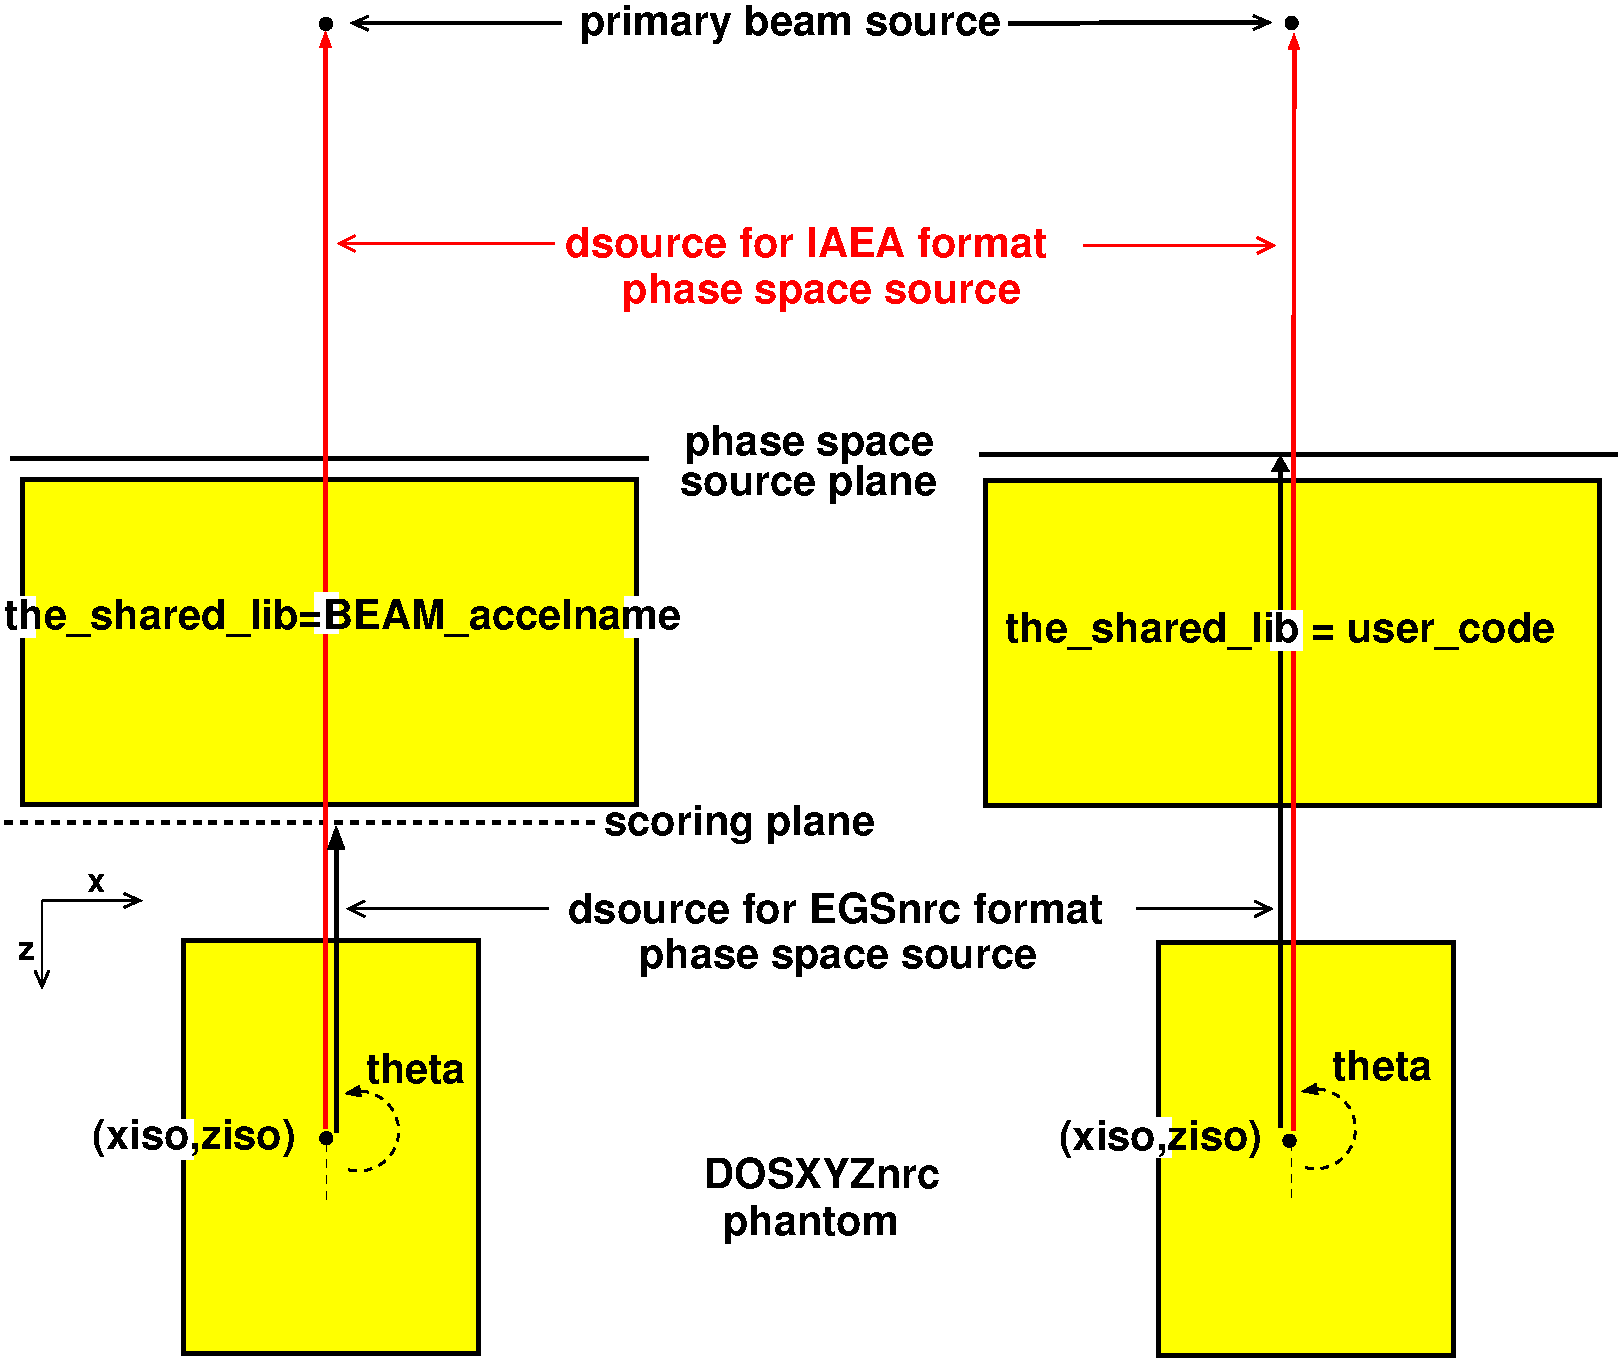
\includegraphics[width=17cm]{figures/src20_1}
\caption{Source 20 incident through a shared library (BEAM or non-EGSnrc user code).  When
the phase space source is run through a BEAM shared library geometry (left), {\tt dsource} defines
the distance between the centre of the scoring plane at the bottom of the geometry and the isocentre (BEAMnrc
phase space source, black arrow), or the distance between the primary source and the isocentre (IAEA phase
space source, red arrow).
When a non-EGSnrc code is used (right), {\tt dsource} defines the distance between the phase space source
and the isocentre (EGSnrc-format phase space source, black arrow) or between the primary source and the isocentre (IAEA phase space
source, red arrow).}
\label{fig_src20_1}
\end{center}
\end{figure}


If a BEAM shared library is used the following conditions apply:
\begin{itemize}
\item The BEAM input file, {\tt the\_input\_file} must define a scoring plane at the bottom of the geometry.  Particle data
at this plane are not actually output but are stored in an internal array for eventual DOSXYZnrc transport through the
phantom.
\item If the source specified in the BEAM input file is a phase space source, it must not make use of the same phase space file as DOSXYZnrc source 20.  This causes a file opening conflict in some versions of
Fortran and will cause the run to fail.  Note that when BEAM is used to define a geometry
for source 20, the BEAM source is not used, so a dummy source of any type can be specified in the BEAM input
file.
\item With a BEAMnrc-format phase space source, the incident Z-position (in the BEAM frame) of the phase space source is
the same as the incident Z-position of the source as defined in the BEAM input file, {\tt the\_input\_file}.  The source 20 input,
{\tt dsource} then defines the distance from the phantom isocentre to the centre of the scoring plane.
\item If an IAEA-format phase space source is used, the incident Z-position of the phase space source is read from
the phase space data itself.  Note that this means the user must ensure consistency between the geometry defined in
BEAM and the incident Z-position of the particles.  The input parameter, {\tt dsource}, defines the distance from
the isocentre to the primary beam source ({\tt i.e.} {\tt dsource}=SAD, see red arrow in figure)
\item The pegs data used in the accelerator simulation is not an input variable and must be the
same as that used in the DOSXYZnrc phantom.
\end{itemize}

If the phase space source is run through a non-EGSnrc shared library (compiled from {\tt user\_code})
the following applies:
\begin{itemize}
\item Phase space data below the defined geometry need not be scored.
\item If a BEAMnrc-format phase space source is used, the incident Z-position (in the {\tt user\_code} frame) is defined
as {\tt dsource}.  Thus, the user must ensure that the source plane is positioned correctly relative to the
defined geometry.
\item For an IAEA-format phase space source, the incident Z-position is read from the phase space source, and
{\tt dsource} defines the primary source-to-isocentre distance.  Again, the user must ensure consistency
between the incident Z-position and the dimensions of the geometry defined in {\tt user\_code}.
\end{itemize}

\indexm{source 20!NRCYCL}
\indexm{source 20!survival ratio}
One issue when running source 20 through a shared library is the determination of how many times
to recycle incident particles so that the phase space source does not rewind, causing loss of information
about particle correlations and subsequent underestimation of dose uncertainties.  As mentioned in Section~\ref{nrcycl}
below, DOSXYZnrc automatically estimates the number of times to recycle each particle, {\tt NRCYCL}, based on
the number of particles in the phase space source, the number of histories requested, and the charge of particles
requested.  However, interactions in the shared library geometry will change the number of particles reaching
the DOSXYZnrc phantom per particle incident from the phase space source.  Thus, the original estimate of
{\tt NRCYCL} is incorrect.  To overcome this when a BEAM shared library is used, an initial calibration comprising
1x10$^6$ particles run through the BEAM geometry only is used to determine the ratio of the number of particles
emerging from the bottom of the BEAM library geometry to the number of incident particles (survival ratio).
{\tt NRCYCL} is then recalculated by multiplying the original estimate by 1/(survival ratio).

\indexm{calflag}
Depending on the shared library geometry, the calibration run can consume
significant CPU time at the beginning of the simulation.  Therefore, if there is a sufficient number of particles in
the phase space source that the user is confident rewinding the source is not an issue, the calibration run can
be skipped by setting the input, {\tt calflag}, to 1.

If a
non-EGSnrc shared library
is used, then the user must provide a routine to estimate the survival ratio of particles passing through the
geometry.  This will be covered in more detail below.

\indexm{synchronized CMs}
When a BEAM shared library geometry includes synchronized component modules (CMs), such as SYNCJAWS, SYNCVMLC or SYNCMLCE,
then the opening coordinates of these component modules (defining the field) can be synchronized with the orientation of the phase space source
plane relative to the phantom.  In this case the value of {\tt MU\_RND}, used to set the incident source orientation (see above), is passed from
DOSXYZnrc to BEAM, where it is then used to set the opening coordinates of any synchronized CMs.
The user controls the synchronization between CM geometries and the incident source orientation using files (one for
each synchronized CM) that associate a field (set of opening coordinates) with a range of fractional monitor units.
See the BEAMnrc Users Manual\cite{Ro09} for more information
about synchronized CMs.

{\bf Non-EGSnrc Geometry Code ({\tt user\_code})}

\indexm{load\_vculib.c}
\index{particleDMLC}
The coding which allows a non-EGSnrc user code compiled as a shared library to communicate with
DOSXYZnrc is found in the C code, {\tt \$HEN\_HOUSE/cutils/load\_vculib.c}. The acronym ``vcu'' stands for
``Virginia Commonwealth University'' and is a reference to the fact that the Lobo and Popescu\cite{LP10}
used a simplified MLC geometry simulation developed at VCU, called {\tt particleDMLC}\cite{Si02}, as a shared
library geometry in simulations with source 20.

\indexm{non-EGSnrc shared library}
\indexm{non-EGSnrc shared library!system requirements}
System requirements for the use of a non-EGSnrc shared library with source 20 (or 21)
are the same as those for a
BEAM simulation source (see Section~\ref{src9sect} above).  Unix/Linux systems must have
a working C/C++ compiler so that {\tt load\_vculib.c} can be compiled to create the
object file, {\tt load\_vculib.o}.  If a working C/C++ compiler is detected on installation
of BEAMnrc/DOSXYZnrc then this is done automatically.  Windows systems do not require
a working C/C++ compiler, since a precompiled version of {\tt load\_vculib.o} is provided.
In addition, the file,
{\tt \$HEN\_HOUSE/specs/dosxyznrc\_config.spec}, where {\tt config} is the configuration
name, must have the
variable {\tt VCULIB\_OBJECTS} set to {\tt \$HEN\_HOUSE/lib/config/load\_vculib.o}
(note that a short form for this is {\tt \$EGS\_LIBDIR/load\_vculib.o})
prior to compiling DOSXYZnrc.  Again, this is set automatically on installation if
{\tt load\_vculib.o} was created successfully.

Currently, {\tt load\_vculib.c} is optimized for calls to subroutines defined in {\tt particleDMLC}. However,
the user can make changes to this file so that it is specific for calls to their own geometry code.  For illustrative
purposes, the following functions must be defined in the user's geometry code, assuming they have made
no changes to {\tt load\_vculib.c} or the DOSXYZnrc coding:

\begin{enumerate}
\indexm{initvcu}
\item{\bf \tt initvcu(char *the\_input\_file, float *survival\_ratio)}
An initialization routine which reads an input file for the geometry code ({\tt the\_input\_file}) and generates
an estimate of the survival ratio of particles between the phase space source and the bottom of the user code
geometry (usually a simulation of an MLC).  The input file would likely specify the geometry parameters and
would also pass the name of the phase space source to the user code.
The survival ratio is used to calculate the number of
times to recycle incident particles, {\tt NRCYCL} (see above).
\indexm{vculib\_sample}
\item{\bf \tt vculib\_sample(float *e, float *x, float *y, float *z, float *u, float *v, float *w, float *wt, int *iq,
 int *latch, int *nhist, int *more\_in\_container)}
A subroutine used to run the geometry code and sample particles reaching the bottom of the geometry.
The subroutine returns the phase space data for a particle at the bottom
of the geometry ({\tt e}=energy; {\tt x,y,z}=particle x,y,z-position; {\tt u,v,w}=x,y,z-direction cosines;
{\tt wt}=particle weight; {\tt iq}=charge; {\tt latch}=latch value), the number of primary histories
run to that point, {\tt nhist}, and an integer, {\tt more\_in\_container}, which is set to 0 if the storage
array for particles reaching the bottom of the geometry is empty ({\tt i.e.} the geometry simulation must
be run on the next call to {\tt vculib\_sample}).
\indexm{vculib\_finish}
\item{\bf \tt vculib\_finish()}
A subroutine called at the end of the simulation to close any files used by the geometry code, free up
reserved memory, etc.
\end{enumerate}

\indexm{source 20!IAEA phase space source}
\label{src20iaeasect}
\subsubsection{IAEA-format phase space sources}

Similar to other phase space sources (sources 2 and 8) source 20 is implemented such that if an IAEA-format phase space source is used, the
incident Z-position of
a particle is automatically read directly from the phase space data.  This eliminates the restriction imposed by BEAMnrc-format
phase space files of all particles being incident in the same plane and, thus, allows more flexibility
in terms of the phase space data that can be used.

\indexm{MU}
\indexm{MU\_RND}
If the IAEA phase space source includes the fractional monitor unit index, {\tt MU}, associated with each particle ({\it i.e.} 4-D data), then
a random value for {\tt MU}, {\tt MU\_RND}, is not chosen at the beginning of each history, and, instead, the value of
{\tt MU} read from the phase space data is automatically
used to set the incident source parameters (isocentre position, incident angle, etc) for the incident particle.
{\tt MU} is automatically
scored in IAEA phase space data output by BEAMnrc simulations using synchronized component modules (CMs) with time-varying opening coordinates
(see the BEAMnrc Users Manual\cite{Ro09}) and can also be included in IAEA phase space data output by DOSXYZnrc
simultions using synchronized sources (20 or 21) by using the {\tt i\_muidx\_out} input flag
(see description of input above and Section~\ref{phspoutsect}).  Thus, use of {\tt MU} read from
the phase space source allows synchronization of source 20 with upstream BEAMnrc simulations having synchronized
CMs or upstream DOSXYZnrc simulations with synchronized sources.

\indexm{spiral CT scan}
\subsubsection{Simulation of Spiral CT Scan}

A recent publication by Kim et al\cite{Ki13} details a modification of Source 8 (See Section~\ref{src8sect} above)
in which the phase space plane can be made to rotate in {\tt phi} about an isocentre which is concurrently
translating in Z, thus simulating exposure in a helical pattern.  Kim et al have used this to simulate dose due
to a spiral CT scan, and their results compare well with measurement.

Spiral scans can be modeled equally well using Source 20 (and 21, see below) using just two control points ({\tt nset}=2).
An example of two control points defining a spiral scan is:

\begin{verbatim}
0, 0, 0, 90, 0, 0, 15, 0
0, 0, 10, 90, 3600, 0, 15, 1.0
\end{verbatim}

These control points define simultaneous translation of the isocentre from {\tt z(1)}=0 to {\tt z(2)}=10 cm and rotation of the source plane
from {\tt phi(1)}=0 at {\tt z(1)} through {\tt phi(2)}=3600$^o$ at {\tt z(2)}.  The angular range, {\tt phi(2)}-{\tt phi(1)}, determines the
pitch of the helix.  In this example, the source rotates ten times (3600$^o$=10$\times$360$^o$) over a Z translation of 10 cm, so the pitch is
equal to 1.  The direction of rotation is determined by the sign of {\tt phi(2)}-{\tt phi(1)}.
If this is positive (as in this example), then rotation is clockwise about the Z-axis; if negative, rotation is counter-clockwise.  Note that the X- and Y-positions of the isocentre in this example remain unchanged, and {\tt theta} is fixed
at 90$^o$, which means the source-isocentre vector is perpendicular to the Z-axis.

The two control points in this example cover the entire range of fractional monitor units ({\it i.e.} {\tt muIndex(1)}=0, {\tt muIndex(2)}=1.0), and, thus,
include all incident particles.
However, using more control points to further subdivide the range, $[$0,1$]$, of fractional monitor units, it would be
possible to generate multiple spiral scans--having different pitch, Z-range, etc--in one simulation.

\subsection{isource = 21: Synchronized BEAM Simulation Source}
\label{src21sect}
\indexm{source routines!isource = 21}
\indexm{source routines!Synchronized BEAM Simulation Source}

Source 21 defines a BEAM treatment head simulation (compiled as a shared library) source incident over multiple ranges
of continuous motion with respect to angle, SSD and isocentre.  The source motion can be synchronized with the settings
of any synchronized component modules (CMs) in the accelerator.  There is also an option to run the source through
a geometry (usually MLC) defined by a non-EGSnrc user code, compiled as a shared library, placed between the treatment
head and the DOSXYZnrc phantom.  Source 21 was developed and contributed by Lobo and Popescu\cite{LP10}.  Just as
source 20 represents a significant enhancement over source 8 (phase space incident from multiple angles), source 21
represents a significant enhancement over source 10 (treatment head incident from multiple angles).

\indexm{source 21!system requirements}
The system requirements for running shared library sources are given in Section~\ref{src9sect} describing source 9 (BEAM
treatment head source incident from one direction).  Instructions on compiling a BEAM accelerator as a shared library
are also given there.

The input parameters for source 21 are:

\begin{description}
\item [~~~~{\tt iqin}]
\indexm{iqin}
Charge of the incident beam (-1: electron, 0: photon, 1: positron, 2: all particle types)
\item [~~~~{\tt isource}] = 21
\item [~~~~{\tt nset}]
\indexm{nset}
\indexm{\$MXANG}
The number of control points defining ranges of continuous source motion.  Same as for source 20 (see above).
{\tt nset} must be in the range 2 $\leq$ {\tt nset} $\leq$ {\tt \$MXANG}, where
{\tt \$MXANG} is defined in
the file {\tt \$EGS\_HOME/dosxyznrc/dosxyznrc\_user\_macros.mortran}.
\item [~~~~{\tt i\_dbs}]
\indexm{i\_dbs}
Set to 1 if directional bremsstrahlung splitting is used in the BEAM simulation and you wish
to reject photons directed outside the splitting field (which will all be fat). Set to 0 otherwise. Note that
{\tt i\_dbs} is read in as a real and converted to integer.
\item [~~~~{\tt e\_split}]
\indexm{e\_split}
Number of times to split charged particles as soon as they enter the phantom geometry. Split particles have their weight reduced by a factor of 1/{\tt e\_split}. This is only used in conjunction with photon splitting ({\tt n\_split}, see Section 8.16) to prevent higher-weight contaminant electrons from compromising statistics in photon beams. For maximum efficiency, it is suggested that you set {\tt e\_split=n\_split}, the photon splitting number.
\item [~~~~{\tt i\_muidx\_out}]
\indexm{i\_muidx\_out}
Set to 1 to include the fractional monitor unit index, {\tt MU}, associated with each particle in IAEA format phase
space output for particles leaving the phantom geometry.  Note that phase space data is not output at all
unless
\indexm{i\_phsp\_out}
{\tt i\_phsp\_out}, the input parameter in the main code controlling phase space output, is set to 1 or 2.
If {\tt MU} is included in the phase space output, then phase space data has a time dimension and is considered 4-D.
Scoring of {\tt MU} allows synchronization between the DOSXYZnrc simulation generating the file and any
downstream simulations--such as BEAMnrc simulations with synchronized component modules--using the file as
a source. See Section~\ref{phspoutsect} for a description of DOSXYZnrc phase space output.
\end{description}

For control points i=1,2,...,{\tt nset}, the following parameters defining the source orientation are entered:
\begin{description}
\item[~~~~{\tt xiso(i)/yiso(i)/ziso(i)}]
\indexm{xiso,yiso,ziso}
x-, y-, z-coordinates of the phantom isocenter.
\item[~~~~{\tt theta(i)}]
\indexm{theta(i)}
Angle of normal connecting origin of the BEAM scoring plane to the isocentre.
\item[~~~~{\tt phi(i)}]
\indexm{phi(i)}
Angle of normal connecting the origin of the BEAM scoring plane to isocentre relative to the +X axis.
\item[~~~~{\tt phicol(i)}]
\indexm{phicol(i)}
2D Angle of rotation of the BEAM scoring plane about its own origin.
\item[~~~~{\tt dsource(i)}]
\indexm{dsource(i)}
The length of the normal from the origin of the BEAM scoring plane to the isocentre.
\item[~~~~{\tt muIndex(i)}]
\indexm{muIndex(i)}
A monitor unit index in the range $[$0,1$]$ defining the fraction of the total number of incident primary histories
delivered up to control point i.  This is slightly different from source 20, where {\tt muIndex(i)} defines the fraction
of incident particles up to control point i.  Thus, for source 21, {\tt muIndex(i)} is actually related to the fractional
monitor units delivered by the BEAM simulation.
Note that {\tt muIndex(i)} $\geq$ {\tt muIndex(i-1)}. Also note that for correct selection of the range
of incident source parameters, {\tt muIndex(1)=0.0} and {\tt muIndex(nset)=1.0}.
\end{description}
This is the end of inputs required for each control point.

\begin{description}
\item[~~~~{\tt the\_beam\_code}]
\indexm{the\_beam\_code}
The name of the BEAM accelerator code ({\it i.e.} {\tt BEAM\_accelname}) used to run the treatment head
simulation.  This must have been compiled as shared library ({\it e.g.} {\tt libBEAM\_accelname.so} on a Linux/Unix system) existing
in your {\tt \$EGS\_HOME/bin/config} directory.
\item[~~~~{\tt the\_input\_file}]
\indexm{the\_input\_file}
The input file for the BEAM treatment head simulation.  This must exist in directory {\tt \$EGS\_HOME/BEAM\_accelname} and must
specify a single scoring plane (usually at the bottom of the accelerator).
\item[~~~~{\tt the\_pegs\_file}]
\indexm{the\_pegs\_file}
The PEGS data to be used in the BEAM treatment head simulation.
\indexm{the\_vcu\_code}
\item[~~~~{\tt the\_vcu\_code}]
This optional input is the name of a non-EGSnrc user code, compiled as a shared library, that can be used to define a geometry
through which particles are run between the bottom of the treatment head and the DOSXYZnrc phantom.  The shared library must
exist in directory {\tt \$EGS\_HOME/bin/config}
\indexm{the\_vcu\_input\_file}
\item[~~~~{\tt the\_vcu\_input\_file}]
Input file for {\tt the\_vcu\_code} defining the geometry interposed between the treatment head simulation and the phantom.
\end{description}

\indexm{\tt MU\_RND}
For each primary history in the treatment head simulation a random fractional monitor unit index, {\tt MU\_RND}$\in[$0,1$]$, is
chosen.  {\tt MU\_RND} is either generated by DOSXZYnrc or, if there are synchronized CMs in the treatment head simulation also
undergoing motion, it is passed to DOSXYZnrc from the BEAM simulation.  More details on the use of synchronized CMs in the BEAM
simulation are given below.  For all particles associated with a given value of {\tt MU\_RND}, the control points, i-1 and i,
within which the source position falls are those for which {\tt muIndex(i-1)}$\leq${\tt MU\_RND}$<${\tt muIndex(i)}, and the
parameters determining the source orientation are calculated using Equation (1) (see Section~\ref{src20sect} above).
Note that, unlike source 20, {\tt MU\_RND} is chosen only for each primary history, not for each incident particle.  Thus,
the {\tt muIndex(i)} for the control points are traceable to actual monitor units in the treatment head.

Recall that the source plane is actually the phase space scoring plane in the BEAM treatment head, defined in {\tt the\_input\_file}.
Phase space data is not output at this plane but is stored in an internal array for use by DOSXYZnrc over the course of the
simulation.

\indexm{i\_dbs}
Similar to source 9 (See section~\ref{src9sect}), since the BEAM simulation is running
concurrently with DOSXYZnrc, if directional bremsstrahlung splitting (DBS) is being used
in BEAM, information about whether or not a particle has been split or has survived
russian roulette (``fat'' particles) is available without having to reconstruct the DBS splitting
field after the fact.  Thus, fat photons can be rejected from the DOSXYZnrc simulation simply
by setting {\tt i\_dbs}=1 and the additional inputs required to reject fat photons from
phase space sources,  {\tt r\_dbs}, {\tt ssd\_dbs}, {\tt z\_dbs} (See Section~\ref{src20sect})
are not required.

\indexm{enflag}\indexm{mode}\indexm{zlast}
As with other phase space and BEAM simulation sources, the input {\tt enflag} must be set
to 2 or 3 to indicate whether {\tt LATCH} bit filtering is to be used, the mode of the
data (with or without {\tt zlast}) being read from the BEAM simulation must be indicated, and
the medium and thickness of the medium surrounding the phantom ({\tt dsurround}) must be
input.  For more information on these inputs, see Section~\ref{sec5}.

\indexm{source 21!use of synchronized CMs}
\subsubsection{Use of synchronized CMs in the BEAM simulation}

If the BEAM treatment head simulation includes synchronized component modules, such as SYNCJAWS, SYNCVMLC, and SYNCMLCE, and
the user is modeling dynamically-changing field coordinates with them, then {\tt MU\_RND} for each primary history is passed
from BEAM to DOSXYZnrc, and the user can synchronize the orientation of the source plane with the field coordinates through
the {\tt muIndex(i)} of the individual control points.  Synchronized CMs are also synchronized with each other.  For more information
on the synchronized CMs, see the BEAMnrc Users Manual\cite{Ro09}.

Figure~\ref{src21_fig} below shows visually how the incident source orientation may be synchronized with the CM settings.

\begin{figure}[htbp]
\begin{center}
\hspace*{-1cm}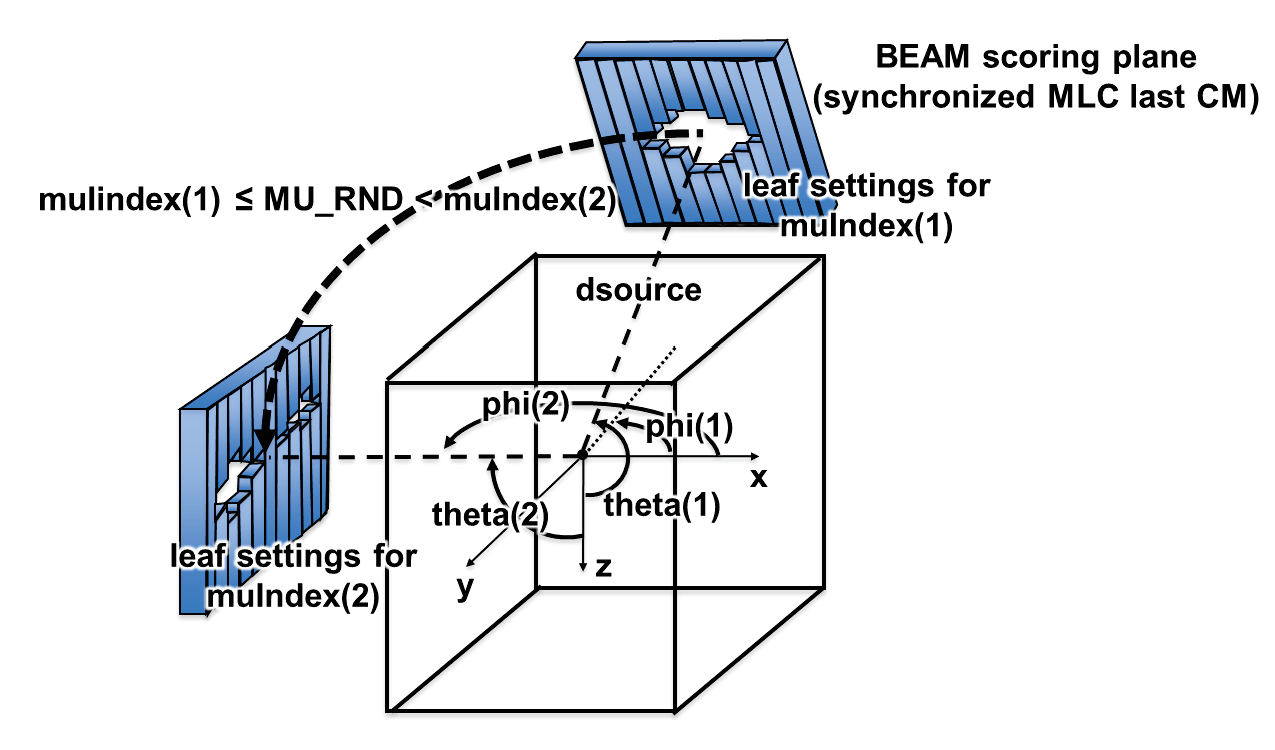
\includegraphics[width=18cm]{figures/src21_fig}
\caption{Source 21, including a synchronized CM, incident on a DOSXYZnrc phantom.  The figure indicates that the final CM in the treatment head
simulation is a synchronized MLC (SYNCVMLC, SYNCMLCE or SYNCHDMLC).  Two control points for the source plane, having different
{\tt muIndex}, {\tt theta} and {\tt phi}, are
indicated.  Different MLC leaf settings are also associated with the values of {\tt muIndex} (the user sets this up in
a file read by the synchronized CM).  Continuous motion of the source between ({\tt theta(1), phi(1)}) and ({\tt theta(2), phi(2)}), along
with dynamic motion of the MLC leaves,
is simulated for values of {\tt MU\_RND} with {\tt muIndex(1)}$\leq${\tt MU\_RND}$<${\tt muIndex(2)}.  Continous motion in
{\tt dource}, isocentre position ({\tt xiso, yiso, ziso}), and the angle of rotation of the source plane in the plane ({\tt phicol}) can
also be simulated.}
\label{src21_fig}
\end{center}
\end{figure}

\indexm{source 21!and non-EGSnrc shared library}
\subsubsection{Running the source through a non-EGSnrc shared library}

\indexm{the\_vcu\_code}\indexm{the\_vcu\_input\_file}
Using the inputs {\tt the\_vcu\_code} and {\tt the\_vcu\_input\_file} the user has the option to interpose another geometry
(usually an MLC) between the source plane and the DOSXYZnrc phantom.  In general, {\tt the\_vcu\_code} is a non-EGSnrc user
code.  Lobo and Popescu\cite{LP10} have used a version of the code particleDMLC\cite{Si02}, developed at Virginia Commonwealth University (hence ``vcu'' in the variable names), to place a simplified MLC simulation between the source and the phantom.

A detailed discussion of potential user codes for creating simplified MLCs is beyond the scope of this manual.  However,
a summary of the subroutines that must exist in {\tt the\_vcu\_code} and the parameters required to communicate
with DOSXYZnrc is given in the description of source 20 (Section~\ref{src20sect}) above.

Note that with source 21, {\tt dsource} always defines the Z-position, in the BEAM frame, of the source plane (scoring plane in the BEAM simulation), and
it is up to the user to ensure that the source is positioned correctly relative to the geometry
defined by {\tt the\_vcu\_code}.


\rfoot[{\sffamily \rightmark}]{{\sffamily \leftmark}}

\section{Other Source-Related Inputs}
\label{sec5}
After the inputs described above, there is another record input with
several other variables related mostly to the source.

\indexm{enflag}
\subsection {{\tt enflag}}
\label{enflag_sect}
The setting of {\tt enflag} determines whether the source is monoenergetic
or has an energy spectrum, or, if the source is a phase space file, whether
or not a dose component is to be calculated.
The possible settings of {\tt enflag} are:
\begin{description}
\item [~~~~= 0] (default) for a monoenergetic source ({\tt isource}=0,1,3,6).
\item [~~~~= 1] for an energy spectrum input ({\tt isource}=0,1,3,6).
\item [~~~~= 2] for a phase space source ({\tt isource}=2) or
full BEAM simulation source ({\tt isource}=9), no dose component
calculation.
\item [~~~~= 3] for a phase space source ({\tt isource}=2) or
full BEAM simulation source ({\tt isource}=9), dose component
calculation using a bit filter (see section~\ref{bitfiltersec} below).
\item [~~~~= 4] for a beam characterization model source ({\tt isource}=4).
\end{description}

\subsection {{\tt mode}}
\indexm{mode}
{\tt mode} only has meaning for a phase space source ({\tt isource}=2).
However, an explicit value for {\tt mode} must exist in the input file
for a full BEAM simulation source ({\tt isource}=9) or
beam characterization model source ({\tt isource}=4), since
{\tt isource}=4 and 9 make use of {\tt medsur}, {\tt dflag} and {\tt dsurround},
which occur after {\tt mode} on the same line.
The possible settings of {\tt mode} are:
\begin{description}
\item [~~~~= 0] (default) the phase space source does not contain
{\tt ZLAST} (for photons, Z of last site of interaction; for electrons,
Z where electron or its ancestor was set in motion by a photon) and, thus,
has 7 variables/record.
\item [~~~~= 2] the phase space source contains {\tt ZLAST} and, thus,
has 8 variables/record.
\end{description}

Note that DOSXYZnrc does not make use of {\tt ZLAST}, but it needs to know
whether {\tt ZLAST} is in the file or not so that the appropriate number
of variables/record can be read.  Thus, if a phase space file is only
going to be used as a source for a DOSXYZnrc calculation, you can save space
by leaving {\tt ZLAST} out of the file.  For more information
about {\tt ZLAST}, see the BEAMnrc Users Manual\cite{Ro09}.

\subsection {{\tt medsur}}
\indexm{medsur}
{\tt medsur} is the medium number for the region surrounding the phantom
as defined by {\tt dsurround}
(see below).  {\tt medsur} is only input for phase space, full BEAM
simulation or beam characterization
model sources ({\tt isource}=2, 4, 8 or 9).  The default setting of {\tt medsur}
is 0, indicating the
surrounding region is vacuum.  However, the user may set this to correspond
to any of the media that they have defined at the top of the DOSXYZnrc input file.
In many cases, the user may wish to fill this region with air and have particles
transported properly through air before reaching the phantom.

\subsection{{\tt dsurround} and {\tt dflag}}
\label{dflagsect}
\indexm{dsurround}
\indexm{dflag}

{\tt dsurround} and {\tt dflag} are required for phase space, full
BEAM simulation and
beam characterization model sources {\tt isource}=2, 4, 8, 9, 10, 20 or 21.
These inputs define the dimensions of the region surrounding the phantom
(ie filled with the medium defined by {\tt medsur}).  Note that
{\tt dsurround} is a 4-dimensional array
with {\tt dsurround(1)} occurring before {\tt dflag} on the input line
and {\tt dsurround(2...4)}, if required, occurring after {\tt dflag}.

The possible settings for {\tt dflag} and their relation to {\tt dsurround}
are as follows:

\begin{description}

\item [~~~~{\tt dflag}=0] (default) {\tt dsurround(1)} defines the thickness
if the surrounding region (in cm) on all sides of the phantom, and the user
need not
input values for {\tt dsurround(2...4)}.  {\tt dsurround(1)}
defaults to 50 cm if it is set $\leq$0.
\item [~~~~{\tt dflag}=1] means that {\tt dsurround(1)} defines the thickness of the
surrounding region in the $\pm$x directions, {\tt dsurround(2)} is the
thickness of the surrounding region in the $\pm$y directions, {\tt dsurround(3)}
is the thickness in the +z direction (bottom of the phantom)
and {\tt dsurround(4)} is the thickness
in the $-$z direction (top of the phantom).  {\tt dsurround(1...4)} default to 0.
\end{description}

Use of {\tt dflag}=1 with {\tt dsurround(1...4)} can save substantial amounts of
computing time if the user is only interested in the dose along a certain axis
or in a specific slice of a DOSXYZnrc phantom (see section~\ref{dsurround_section}
below).

\subsection{{\tt ein}}
\indexm{ein}

{\tt ein} is the kinetic energy of
a monoenergetic incident beam in MeV.  It defaults to 1.25 MeV if
{\tt ein} is set $\leq$ 0.  Note that {\tt ein} is only required if
{\tt isource}=0,1,3,6 and {\tt enflag}=0.

\subsection{{\tt FILNAM}}
\indexm{FILNAM}

{\tt FILNAM} is the file name (with extension) of:

\begin{description}
\item[incident beam energy spectrum] if {\tt isource}=0,1,3 or 6 and
{\tt enflag}=1.  In this case, {\tt FILNAM} has a specific format which
corresponds to the ensrc format used in the original EGSnrc system
\indexm{energy spectrum format}
(see {\tt \$HEN\_HOUSE/spectra} for a large number of
example spectra):

{\tt ENSRC.V5 File format\\
====================}
\begin{tabbing}
\= {\tt SPEC\_TITLE} \\
\> {\tt NENSRC, ENMIN, IMODE} \\
\> {\tt ENSRCD(I), SRCPDF(I) (I = 1 to NENSRC)} \\
\end{tabbing}
\vspace*{-5mm}
where:
\vspace*{-3mm}
\begin{description}
\item [~~~~{\tt SPEC\_TITLE}] is an 80-character spectrum title
\item [~~~~{\tt NENSRC}] = \# of energy bins in the spectrum histogram
\item [~~~~{\tt ENMIN}] = lower energy of first bin in MeV
\item [~~~~{\tt IMODE}] Set to 0 for histogram counts/bin; set to 1 for
counts/MeV
\item [~~~~{\tt ENSRCD(I)}] = upper energy of bin I in MeV
\item [~~~~{\tt SRCPDF(I)}] = probability of finding a particle in bin
I (SRCPDF
need not be normalized)
\end{description}

\item[phase space source:] if {\tt isource}=2 or 8 and {\tt enflag}=2 or 3.
See Section~\ref{source2sect} for more details.
\item[beam characterization model:] if {\tt isource}=4 and {\tt enflag}=4.
\indexm{the\_beam\_code}
\indexm{the\_input\_file}
\indexm{the\_pegs\_file}
\item[{\tt the\_beam\_code}, {\tt the\_input\_file}, {\tt the\_pegs\_file}:]
if {\tt isource}=9 or 10 and {\tt enflag}=2 or 3.  These are the names of the
BEAM accelerator code being used as a source, the input file for the BEAM
simulation, and the pegs data for the BEAM simulation respectively.  See
section~\ref{src9sect} for more details.
\end{description}

\subsection{{\tt IOUTSP}}
\indexm{IOUTSP}
{\tt IOUTSP} is only required with an incident energy spectrum ({\tt enflag}=1).  The
possible settings of {\tt IOUTSP} are:

\begin{description}
\item [~~~~= 0] (default) no output summary of incident energy spectrum
in {\tt .egslst}.
\item [~~~~= 1] output a summary of the incident energy spectrum to the
{\tt .egslst} file.
\end{description}

\section{Phase Space Sources}
\index{phase space sources}

The phase-space files output by BEAMnrc and used by DOSXYZnrc for sources 2 and 8 are
described in detail in section 7 of the BEAMnrc User's Manual.
\cite{Ro04a}.

The phase-space files are binary files  opened with ACCESS = 'direct' and
FORM = 'unformatted'.  Because they are binary files, and because there
are two common byte orders used for binary files by different systems
(eg PCs and DEC machines use one form and SUNs and SGIs use the other),
files written by one system may not be compatible with another system.
The utility {\tt readphsp} found on {\tt \$OMEGA\_HOME/progs/readphsp} can
convert files from one format to the other (see the description in the BEAMnrc
User's Manual. \cite{Ro04a}.)

There are also two types of phase-space files determined by how many
variables they contain.  The shorter format is
called '{\tt MODE0}' and  {\tt ZLAST} is not
scored and the longer format is
'{\tt MODE2}' when {\tt ZLAST} is present.  Since DOSXYZnrc makes no use of
the {\tt ZLAST} variable, it saves space to use {\tt MODE0} files for use with
DOSXYZnrc.  The '{\tt MODE0}' or '{\tt MODE2}'
designation appears in the first record of a phase-space file along
with the total number of particles contained in the file, the number
of photons, maximum energy of any particle in the file,
minimum energy of electrons, and minimum energy of
photons.

\indexm{phase space sources!negative energy marker}
\indexm{phase space sources!using old files}
\indexm{uncertainties}
\indexm{statistics}
Phase space files generated by BEAMnrc use negative
{\tt E} (energy) to mark the first particle scored by each new primary
history.  If the file is used as a source, then the negative {\tt E} marker
allows scored quantities (ie energy deposited) to be grouped according
to primary history.  This ensures that uncertainties estimated account
for the correlations between incident particles in a phase space
source~\cite{Wa02a}.  If an old phase space file without negative {\tt E} markers is used
as a source, then scored quantities will be grouped according to incident
particle instead of primary history.  DOSXYZnrc will then output a warning
that uncertainty may be underestimated because correlations between incident
particles could not be taken into account.  This is not a cause for concern,
because we have found~\cite{Wa02a} that in the cases we studied,
the underestimate is not significant.

When using a phase space source, if the entire phase space file is read
before the requested number of histories is run, then DOSXYZnrc restarts
the phase space file from the beginning.  For the reasons discussed in
section~\ref{nrcycl}, page~\pageref{nrcycl}, this is not a desirable
occurrence and one should strive to avoid this by using the recycling
feature (which also saves on reading time).

\index{IAEA-format phase space sources}
\label{iaeaphspsect}
\subsection{IAEA-format Phase Space Sources}

In addition to the standard BEAMnrc phase space files described
above, DOSXYZnrc can
also use IAEA-format phase space data as a source.  This allows the
user to make use of IAEA's online data base of accelerator phase space
data at:\\
\htmladdnormallink{www-nds.iaea.org/phsp/phsp.htmlx}{http://www-nds.iaea.org/phsp/phsp.htmlx}

\index{C++ compiler}
Note that this functionality requires that EGSnrc/DOSXYZnrc be installed on a machine
with a working C++ compiler.  This is detected automatically during
EGSnrc installation and, if a working C++ compiler is found, the library
of IAEA phase space handling routines is compiled.

\index{{\tt .IAEAheader}}
\index{{\tt .IAEAphsp}}
\index{IAEA phase space data! header file}
\index{IAEA phase space data! phase space data file}
Phase space data in IAEA format comprises both a header
(extension {\tt .IAEAheader}) file and a phase space data
(extension {\tt .IAEAphsp}) file.  When using IAEA phase space data as
a source, only the full name and directory path of the {\tt .IAEAphsp} file needs to be specified
(See Section~\ref{source2sect}).  The {\tt .IAEAheader} file is assumed to be
in the same directory.

Note that when IAEA phase space sources are used the incident Z-position of each particle
is available and is automatically read, either from the header file in the case of
planar phase space data (such as that scored by BEAMnrc), or from the phase space
data itself if it is scored in 3-D (such as that scored by DOSXYZnrc).  The ability to handle
3-D phase space data greatly enhances the flexibility of DOSXYZnrc and allows it to
use non-planar data supplied by manufacturers, such as that supplied by Varian for
their TrueBeam accelerators.  In addition, IAEA phase space files generated by BEAMnrc simulations
with synchronized component modules (CMs) and by DOSXYZnrc simulations using synchronized
sources (20 or 21) may include the fractional monitor unit ({\tt MU}) associated with each particle.
This is automatically read in and used by DOSXYZnrc's synchronized phase space source (source 20) allowing
synchronization between the DOSXYZnrc simulation and the upstream simulation that generated the phase
space file.  See Sections~\ref{src2iaeasect} and \ref{src20iaeasect} for more information.

Form more information on the format of IAEA phase space data, see the
BEAMnrc Manual and IAEA Report INDC(NDS)-0484\cite{CJ05}.

\section{Calculating Dose Components with DOSXYZnrc}
\label{bitfiltersec}
\subsection{Bit Settings}
\indexm{bit setting}

\indexm{LATCH}
The {\tt LATCH} variable, associated with each particle in a
BEAMnrc simulation, is a
32-bit variable used to track the particle's history.  It is discussed in
detail in the BEAMnrc User's Manual \cite{Ro04a}.

Each bit in {\tt LATCH} is designated as follows with bit 0 being the lowest value bit:
\begin{description}
\item [~~~~bit 0] Set to 1 if a photon is created by a bremsstrahlung event or an electron is created by a bremsstrahlung photon; 0
otherwise
\item [~~~~bits 1-23] Used to record the region where a particle has been and/or
has interacted. Note that the bit set for a region is determined by
{\tt IREGION\_TO\_BIT} (which is defined in the BEAMnrc simulation)
for that region.
\item [~~~~bits 24-28] Stores {\tt IREGION\_TO\_BIT} (as a binary number) of the
region in which a secondary particle
is created; if these bits are all 0, the particle is a primary
particle
\item [~~~~bits 29-30] Store the charge of a particle at the time {\tt LATCH} is output
\indexm{LATCH}
to a phase-space file.
\item [~~~~bit 31] Set to 1 if a particle has crossed a scoring plane
more than once when {\tt LATCH} is output to a phase-space file.
\indexm{LATCH}

\end{description}

For secondary particles, recording the {\tt IREGION\_TO\_BIT}'s of
the regions in which they were
created in bits 24-28 is equivalent to multiplying the {\tt IREGION\_TO\_BIT} by
2$^{24}$, or 16777216.  Thus, to retrieve {\tt IREGION\_TO\_BIT} of the region
of origin of a
secondary particle, the {\tt LATCH} value of the particle must be divided by
16777216 (i.e., taking the value {\tt INT(LATCH/16777216)}).
\indexm{LATCH}

When used with a phase space source, DOSXYZnrc has the
capability of selecting from the phase space file only those particles that
have user-specified bits (called a ``bit filter") set in their {\tt LATCH}
variables.
Thus, DOSXYZnrc will score only the dose component arising from these user-selected
particles.  For example, in the BEAMnrc simulation, bit 10 may be associated
with a square applicator, so any particle in the phase space file that has
been in the applicator will have bit 10 set in {\tt LATCH}.  When using
this phase space file as a source in DOSXYZnrc, the user may opt to use only
those particles that have bit 10 set, thus scoring the dose component from
particles that have been in the applicator.

In general, a dose component can be selected
according to what regions particles have passed through/interacted in,
whether the particle is a primary or secondary, if the particle is a
secondary then where it was created, and any combination of these.

\subsection{Input for Dose Component Calculations}

In order to enable dose component calculations with a phase space source
or full BEAM simulation source
({\tt isource}=2, 8 or 9),
the variable {\tt enflag} must be set to 3.  The user then specifies which
\indexm{enflag}
type of bit filter ({\tt I\_BIT\_FILTER}) to use.  Below is a description of the
4 types of bit filters available and the inputs associated with each.

\begin{description}
\indexm{I\_BIT\_FILTER}
\indexm{NBIT1}
\indexm{NBIT2}
\indexm{BIT}
\index{IREGION\_TO\_BIT}
\item [{\tt I\_BIT\_FILTER}=0] This is an inclusive/exclusive bit filter.  On the
same line as {\tt I\_BIT\_FILTER}, the user inputs the integers {\tt NBIT1} and
{\tt NBIT2}.  {\tt NBIT1} is the number of bits to include and {\tt NBIT2} is
the number of bits to exclude.  Restriction is that
0$\leq${\tt NBIT1}+{\tt NBIT2}$\leq$29.
Both {\tt NBIT1} and {\tt NBIT2} can be set to zero.  On the next line, the
user inputs {\tt BIT(I) (I=1,NBIT1)}, the bits to be included, and on
the following line \\ {\tt BIT(I) (I=NBIT1+1,NBIT1+NBIT2)}, the bits to
be excluded.  If any of the first set of {\tt NBIT1} bits are set and none
of the second set of {\tt NBIT2} bits are set in the particle's {\tt LATCH}
variable, the particle is used in the
simulation.

\item [{\tt I\_BIT\_FILTER}=1] This is an exclusive bit filter.  On the same line
as {\tt I\_BIT\_FILTER}, the user inputs the integer {\tt NBIT1}, the
number of bits to be excluded (0$\leq${\tt NBIT1}$\leq$29).  {\tt NBIT2} is
not relevant for this filter and is automatically set to 0.  On the
next line, the user inputs, {\tt BIT(I) (I=1,NBIT1)}, the bits to
be excluded.  If any of these {\tt NBIT1} bits are set in the particle's
{\tt LATCH} variable, the particle
is NOT used in the simulation.

\item [{\tt I\_BIT\_FILTER}=2] An inclusive region-of-origin filter.
The user inputs {\tt NBIT1} on the same line
as {\tt I\_BIT\_FILTER}, where {\tt NBIT1} is the number of regions of origin
to be included.  Since regions of origin are distinguished only by their
values of {\tt IREGION\_TO\_BIT}, {\tt NBIT1} can also be seen as the
number of distinct values of {\tt IREGION\_TO\_BIT} to be included. The
restriction on {\tt NBIT1} is 0$\leq${\tt NBIT1}$\leq$24.  {\tt NBIT2} is
not relevant for this filter and is automatically set to 0.  On the
next line, the user inputs {\tt IREGION\_TO\_BIT(I) (I=1,NBIT1)}, the
{\tt IREGION\_TO\_BIT} values of the {\tt NBIT1} regions of origin to
be included.  If the particle originated in any one of these {\tt NBIT1}
regions, then it will be used in the simulation.  Primary particles will be included if
{\tt IREGION\_TO\_BIT=0} is one of the {\tt NBIT1} values of
{\tt IREGION\_TO\_BIT} to include.

\item [{\tt I\_BIT\_FILTER}=3] An exclusive region-of-origin filter.
The user inputs {\tt NBIT1} (0$\leq${\tt NBIT1}$\leq$24), the number of
regions of origin to be excluded, on the same line as {\tt I\_BIT\_FILTER} and
ignores {\tt NBIT2}, since it is not relevant for this filter.  On the
next line the user inputs {\tt IREGION\_TO\_BIT(I) (I=1,NBIT1)}, the
{\tt IREGION\_TO\_BIT} values of the regions of origin to be excluded.
If a particle originated in any one of these regions, then it is NOT
used in the simulation.  Note that primary particles will be excluded if
{\tt IREGION\_TO\_BIT=0} is one of the {\tt NBIT1} values of
{\tt IREGION\_TO\_BIT} to exclude.

\end{description}

Note that since only one bit filter can be input per simulation, only one
dose component may be calculated at a time using DOSXYZnrc.  This is because
of the large memory requirements for the dose scoring arrays.

\section{Other Input Variables}

This section provides descriptions of main DOSXYZnrc input variables not
covered above.

\vspace*{-0.5cm}
\subsection{{\tt IPHANT}}
\label{iphantsect}
\indexm{IPHANT}

If {\tt IPHANT} is set to 1, DOSXYZnrc outputs phantom data to
a {\tt .egsphant} file.  This file has the same format as the
{\tt .egsphant} file that {\tt ctcreate} outputs for CT data
(see section~\ref{egsphantsect}) and can be read by
{\tt dosxyz\_show}\cite{Ka98},
along with the {\tt .3ddose} dose output file to display isodose contours in
the phantom.  Note that this option is redundant (and, therefore, unavailable)
when using a CT phantom because it is an input file from ctcreate).

\subsection{{\tt MAX20}}
\indexm{MAX20}
\label{MAX20description}

When {\tt MAX20} is set to 1, a summary of the maximum 20 doses in the
phantom is output to the screen (log file) and list file.  This summary
includes an output of the 20 maximum doses with their fractional
uncertainties and coordinates, the average of the 20 maximum doses, the average
fractional uncertainty of these doses (not the uncertainty of the average), the
average fractional uncertainties of all doses $>$ 50\% of the maximum dose,
and the average absolute uncertainty of all doses $>$ 50\% of the maximum dose
as a fraction of the maximum dose.

When not in CT phantom mode, {\tt MAX20} is the last variable on the line(s)
specifying the regions for which dose will be output (ie record 9).  If
{\tt MAX20} is set to 1 on ANY ONE of these lines (including the line of
zeros indicating the end of this record) then the summary of the 20 maximum
doses will be output.

In CT phantom mode, {\tt MAX20} is input
\indexm{MAX20} on the same line as {\tt zeroairdose} and {\tt doseprint}.

This option is useful for timing/efficiency studies.
\subsection{{\tt zeroairdose}}
\indexm{zeroairdose}
\label{zeroairdose}

{\tt zeroairdose} is only used in CT phantom mode.
Setting {\tt zeroairdose} to 1 will set all dose estimates in
voxels with density $<$ 0.044 g/cm$^3$ to zero in the {\tt .3ddose}
\indexm{.3ddose}
\indexm{files!.3ddose}
file.  This has the effect of zeroing dose in voxels filled with air
(see the default CT ramp in Figure~\ref{fig_ct02}--note that ``AIR''
has a density ranging from 0.001-0.044 g/cm$^3$).
Air dose will not be zeroed in the {\tt .egslst} file, this file will
continue to report the precise estimated dose.  {\tt zeroairdose} serves
as a dose visualisation parameter for CT phantom simulations, since, in general, the user is only interested
in seeing the dose within the patient, not in the surrounding air.

\subsection{{\tt doseprint}}
\indexm{doseprint}

This input parameter is also only used in CT phantom mode.

{\tt doseprint} is set to 1 if the user wants a full output of doses in
all voxels of the CT phantom in the {\tt .egslst} file.  Since, in CT
phantom cases, the user is usually not interested in this output and, owing
to the large number of voxels in a CT phantom, it can make the {\tt .egslst}
exceptionally large, the default is to suppress this output (ie set
{\tt doseprint} to 0).

\subsection{{\tt NCASE}}
\indexm{NCASE}

{\tt NCASE} is the number of histories to run in a simulation.  Minimum
value is 100.  Default is 100 if {\tt NCASE} is set $<$ 100.  The number
of histories per output batch is equal to {\tt NCASE}/({\tt \$NBATCH}),
where {\tt \$NBATCH} is currently set to 10.

\subsection{{\tt IWATCH}}
\indexm{IWATCH}

{\tt IWATCH} controls output to the screen (interactive run) or to the
{\tt .egslog} file (batch run) during beam execution.  The possible settings
are:
\begin{description}
\item [~~~~= 0] (default) On completion of each batch, outputs information about the
batch (eg elapsed time, CPU time, elapsed/CPU time, random number used
to begin batch, \# of random seeds used in the batch, total number of
histories run up to and including the current batch, the total number of
particles scored in the first phase-space file)

\item [~~~~= 1] Outputs same information as 0 plus, after every particle
interaction, outputs complete information about the particle(s)
involved (eg interaction type, particle type, position of particle on
stack, particle energy, X-Y-Z position of particle, U-V-W direction
cosines, {\tt LATCH} value of particle, region \# of particle); also informs
\indexm{LATCH}
user when a particle is being discarded, when a particle is passing from
one CM to another

\item [~~~~= 2] Similar to 1 but with complete particle information output at
every step; also outputs total dose in a region whenever energy is
deposited there

\item [~~~~= 3] Similar to 2 but with particle and dose information output
whenever dose is deposited.

\item [~~~~= 4] Outputs same information as 0 plus {\tt .egsgph} and {\tt
.egsgeom} files for graphical representation of the accelerator and
particle paths using {\tt EGS\_Windows.}
\indexm{.egsgph}
\indexm{.egsgeom}
\indexm{files!.egsgph}
\indexm{files!.egsgeom}
\end{description}

\subsection{{\tt TIMMAX}}
\indexm{TIMMAX}

{\tt TIMMAX} is the maximum CPU time in hours allowed for a simulation.
{\tt TIMMAX} defaults to 0.99 hrs if it is set = 0.  However, this time-restriction function is not activated in the current version of DOSXYZnrc except to
print a warning as it starts a batch which will exceed this limit.


\subsection{{\tt INSEED1, INSEED2}}
\indexm{INSEED}
\indexm{RANMAR}
\indexm{RANLUX}
\indexm{random number generator}
\indexm{random number seeds/pointers}

These are random number seeds used to initialize the
RANMAR\cite{MZ91,Ma90a} or RANLUX\cite{La94,Ja94}
random number generator.  Within DOSXYZnrc,
{\tt INSEED1} is limited
to the range\\ 0$<${\tt INSEED1}$\leq$31328
(defaults to 1802), and {\tt INSEED2} has
the range 0$<${\tt INSEED2}$\leq$30081 (defaults to 9373).  These
ranges/defaults are designed for RANMAR (the default random number generator),
however, if
you are using RANLUX then {\tt INSEED1} is the ``luxury level"
of the random number generator and must be in the range
0$<${\tt INSEED1}$\leq$4, otherwise, it will automatically be set to the
default luxury level of 1 (Note: this means that the DOSXYZnrc default value
for {\tt INSEED1} of 1802 will ultimately get reset to 1 by RANLUX).

Note that \verb+INSEED1+ and \verb+INSEED2+ are only used to initialize
the random number generator, and, during a simulation, they no longer
reflect the values of the seeds that are actually used to generate
the random numbers.
When resuming
({\tt IRESUME} = 1), the state of the random number generator at the end
of the previous run is read from the {\tt .egsdat} file and is used when the
simulation resumes.
Thus, a resumed run with a total of
10000+10000 histories should generate results identical to a single run
of the same simulation with 20000 histories.  Also note that
when running parallel jobs
with DOSXYZnrc (see section~\ref{parallelcalc}), {\tt INSEED2} must have
a different value for each of the individual jobs that make up the simulation.
This is taken care of automatically if you use DOSXYZnrc's built-in
parallel processing functionality.

\index{random number generator! switching from RANMAR to RANLUX}
In order to switch from the RANMAR random number generator to RANLUX in
DOSXYZnrc, go into {\tt \$EGS\_HOME/dosxyznrc/Makefile} and
change the line:
\begin{verbatim}
RANDOM = $(EGS_SOURCEDIR)ranmar
\end{verbatim}
to:
\begin{verbatim}
RANDOM = $(EGS_SOURCEDIR)ranlux
\end{verbatim}
Then recompile DOSXYZnrc.

\subsection{{\tt BEAM\_SIZE}}
\indexm{BEAM\_SIZE}

{\tt BEAM\_SIZE} allows the user to control the maximum beam size for phase space sources (sources 2,
8, 20), BEAM simulations sources (souces 9, 10, 21) and the beam model source (source 4).
{\tt BEAM\_SIZE} is the side of a square field in cm. The default value for {\tt BEAM\_SIZE} is 100 cm.
Particles are discarded immediately if they are outside the
square defined by {\tt BEAM\_SIZE} centred on the beam axis in the source scoring plane.

One should be careful with the use of this parameter because particles outside
the specified field (defined by {\tt BEAM\_SIZE)} may have some effects on the dose
distributions calculated and therefore the results may be biased with the use
of {\tt BEAM\_SIZE} smaller than the field size of the original phase-space data. It
should also be noted that this parameter cannot be used as a beam defining tool,
such as a collimator,
because in reality particles outside of the inner opening of any beam confining
components may interact with and be scattered by the components,  resulting in
an increase of the particles within the specified field.

\subsection{{\tt ISMOOTH}}
\label{ismooth}
\indexm{ISMOOTH}

\indexm{re-use of phase space}
When phase-space data are used DOSXYZnrc will re-use the phase-space particles if
\indexm{phase-space input}
the number of histories required by the user is greater than the number of
particles stored in the phase-space file. Clearly, the dose distributions
obtained with more histories have smaller statistical uncertainties.
Although some histories may start with the same incident phase-space, the
particle trajectories will be different because different random numbers will
be used in the simulations in the phantom, resulting in different dose
distributions. However, surface doses are mainly affected by the electron
fluence distribution and therefore would not be improved by re-using the
phase-space particles if the data file contains too few particles
(i.e., the calculated doses
would have small statistical uncertainties but large systematic uncertainties).

In order to reduce the systematic uncertainties due to a small data set,
DOSXYZnrc can re-distribute the phase-space particles {\bf as long as the
simulated linear accelerator geometry is symmetric,  and the treatment
field is centred on the beam axis}. Currently, DOSXYZnrc is allowed to move a
particle  to 3 symmetrical positions (each with modified direction
cosines). This process is accurate as long as the phase space file is
symmetric with respect to the x-axis and also with respect to the
y-axis.  Suppose a particle is at (x,y) with (u,v) the 3 new positions
are
\begin{center}
(-x,y) with (-u,v), \\
(x,-y) with (u,-v), \\
(-x,-y) with (-u,-v)
\end{center}
%%Dave commented the following out since even after corrections, he
%is not at all convinced it is right.
%If further, their is a square symmetry (eg if no jaws are included in the
%simulated linear accelerator geometry or they are all on the same level),
%one can further move the particle
%to 4 other positions (one needs to modify DOSXYZnrc in order to do so), i.e.,
%
%\begin{center}
%
%(x,y) with (-u,-v),
%
%(-x,y) with (u,-v),
%
%(x,-y) with (-u,v),
%
%(-x,-y) with (u,v)
%\end{center}
A user has two options for {\tt ISMOOTH}:
\indexm{ISMOOTH}
\begin{description}
\item [~~~~= 1] DOSXYZnrc re-distributes the phase-space particles when they are used more than once.


\item [~~~~= 0] (default) DOSXYZnrc re-uses the phase-space particles without changing the particle positions

\end{description}
\indexm{re-use of phase space}

See also section~\ref{nrcycl} which discusses recycling phase space data.

\subsection{{\tt NRCYCL}}
\label{nrcycl}
\indexm{NRCYCL}
\indexm{phase space source!recycle}

{\tt NRCYCL} is an essential input when using a phase space source. It
determines the number of times that each particle from a phase space
source is recycled ({\em  ie}, reused each time it is read).
If {\tt NRCYCL}$>$0, then
each source particle is used a total of {\tt NRCYCL} + 1 times
before moving on to the next particle in the source.
When phase space data is sparse, then particles must be re-used to obtain
adequate statistics.  In addition to recycling, particles may also
be re-used whenever a phase space source is restarted
(happens automatically when the simulation has reached
the end of the source).  Restarting is not recommended, however,
because it may lead to underestimates of the uncertainty in the
final results~\cite{Wa02a}.  We recommend setting {\tt NRCYCL} to a value
that will ensure that the entire phase space source gets sampled (ie
the simulation uses almost all the particles in the source) but
prevents the source from being restarted.

If you are unsure of
the correct value of {\tt NRCYCL} to use, then
run with {\tt NRCYCL}=0 and DOSXYZnrc will automatically calculate
a value of {\tt NRCYCL} based on the number of histories and
the number of particles (with appropriate charge) in the phase space source.
There is a possibility
that, even with the automatically calculated value of {\tt NRCYCL},
the phase space source will restart.  This may be due to particles
that have been rejected because they missed the geometry, were multiple
passers and/or were beyond the beam field defined by {\tt BEAM\_SIZE}) or
else the algorithm for calculating {\tt NRCYCL} may have determined that
setting {\tt NRCYCL}$>$ 0 will result in the phase space source not being
sampled adequately.
If the
source has only been restarted once and only a small fraction of it
has been covered on the second pass, this is not likely to have a significant
impact on the estimated uncertainties.  However, if a large portion of the
source is covered on the second pass, or if it is restarted more than once,
we recommend re-running the simulation with a new value of
{\tt NRCYCL} calculated as:
\begin{eqnarray}
\label{nrcycleqn}
{\tt
NRCYCL}=
\frac{{\tt NCASE}}{\left({\tt NPHSP - (NSMISS/NRCYCL}_{prev}) - {\tt NOUTSIDE - NRJCT - NDBSRJCT}\right)}-1
\end{eqnarray}
where {\tt NCASE} is the number of incident histories, {\tt NPHSP} is the
total number of particles in the phase space file, {\tt NSMISS} is
the number of particles that missed the geometry in the previous run,
{\tt NRCYCL$_{prev}$} is the setting of {\tt NRCYCL} in the previous run,
{\tt NOUTSIDE} is the number of particles rejected because they were
outside the field defined by {\tt BEAM\_SIZE} in the previous run,
{\tt NRJCT} is the number of particles rejected because they were
multiple passers in the previous run, and {\tt NDBSRJCT} is the number of
photons rejected because they fall outside the directional bremsstrahlung
splitting (DBS) field radius at the SSD (only if DBS was used in the BEAM
simulation that generated this source AND the user has opted to reject
these photons--see section~\ref{source2sect} for more information about
this).  Note that {\tt NPHSP}, {\tt NSMISS}, {\tt NOUTSIDE},
{\tt NRJCT} and {\tt NDBSRJCT} are all available from the {\tt .egslst} file of the previous run.
Always round your calculated value of {\tt NRCYCL} up to the nearest integer.
\indexm{DBS}
\indexm{NRCYCL}

{\tt NRCYCL} is not automatically calculated if you are only using the
positrons in the phase space source or if you are selecting a sub-set of
the phase space source based on {\tt LATCH} settings.  In these cases,
the information required for an a-priori calculation of {\tt NRCYCL}
is not available in the header of the phase space source.
We recommend setting {\tt NRCYCL} manually to a ``best guess" value.  Then,
if the source restarts, calculate {\tt NRCYCL} using Equation~\ref{nrcycleqn}
where {\tt NRJCT} includes the number of particles rejected because they
were multiple passers, the number of particles rejected because they were
the wrong charge and the number of particles rejected because they did not
have the right {\tt LATCH} setting.

If the phase space source is stored on a remote disk, then using
{\tt NRCYCL} to avoid restarting a phase space source also has
the beneficial effect of reducing network traffic
because it reduces the number of times that a phase space
source is accessed during a run (particle data is stored in temporary
variables during recycling, not re-read from the source).  Repeated
accessing of a phase space source on a remote disk can slow a simulation
down considerably.

{\tt NRCYCL} is compatible with {\tt ISMOOTH} (see section~\ref{ismooth}).
So if {\tt ISMOOTH}=1, then,
during the recycling loop, the initial position and direction cosines of
the particle are shifted according to the scheme outlined in the
{\tt ISMOOTH} subsection above.
\indexm{ISMOOTH}
\indexm{NRCYCL}

Note that the total number of histories is
always limited by {\tt NCASE}.  For example, if the
phase space source has 1000 suitable particles and the user sets {\tt NRCYCL}=9
(so each particle will be used a total of 10 times), but only sets
{\tt NCASE}=5000, then the simulation will only have a chance to use (and
recycle) the first 500 particles before the simulation stops.  In order to
go through the entire phase space source, the user would have to set
{\tt NCASE}=10000.  If {\tt NCASE}$>$10000 then the phase space source
would be restarted at least once during the run.  After restarting, particle
recycling continues as before.

\subsection{{\tt IRESUME}}
\label{iresumesect}
\indexm{IRESUME}
\indexm{resuming}

\indexm{.egsdat}
The possible settings of {\tt IRESUME} are:
\begin{description}
\item [~~~~= 0] (default) DOSXYZnrc initiates a new run, deleting all of the output
files ({\tt .egslog,} {\tt .egslst}, {\tt .egsdat}, \etc) if present
\item [~~~~= 1] Resume a previous run; DOSXYZnrc opens the
{\tt .egsdat} from the previous run and reads:
\begin{enumerate}
\item $\sum_{i=1}^{nhist}edep_i$ and $\sum_{i=1}^{nhist}edep_i^2$ for
all voxels, where {\tt edep$_i$} is energy deposited by primary (non-phase space)
history i
and {\tt nhist} is the number of primary histories in the previous run.
\item number of histories and number of primary histories from the previous run
\item the time taken by the previous run
\item the state of the random number generator at the end of the
previous run
\item other data relating to particle fluence in previous run, number of
electron steps, number of particles rejected from phase space source (if
applicable), etc.
\end{enumerate}
After the current run is complete, dose and
uncertainties are calculated using data from the current run and from
the previous run~\cite{Wa02a}.  Note that the
number of histories to run and the total CPU time allowed for the
simulation do not include the histories and CPU time from the previous run.
Also note that, currently, although a resumed simulation with, for example
100000+100000 histories will have identical dose results to a one-off
simulation
with 200000 histories, the uncertainty estimates on the doses may not be
the same.  We are currently investigating why this is so.
\item [~~~~= 2] DOSXYZnrc creates the {\tt .egsinp} file and then exits without
running the simulation
\item [~~~~= 3] DOSXYZnrc opens the {\tt .egsdat} file from a previous run,
reads the data enumerated above and calculates doses and uncertainties;
no simulation is run.
\indexm{.pardose}
\item [~~~~= 4] DOSXYZnrc recombines the binary {\tt .pardose} files from
parallel jobs and creates {\tt .egslst} and {\tt .3ddose} output
files from the recombined data (see section~\ref{parallelcalc} for
more about parallel jobs).
\end{description}

\subsection{{\tt IDAT}}
\label{idatsect}
\indexm{IDAT}
\indexm{files!.egsdat}
\indexm{.egsdat}

The possible settings of the variable {\tt IDAT} are:
\begin{description}
\item [~~~~= 0] (default) DOSXYZnrc outputs {\tt .egsdat} file with
resume data after every batch.
\item [~~~~= 1] DOSXYZnrc does not output a {\tt .egsdat} file at all.
\item [~~~~= 2] DOSXYZnrc outputs a {\tt .egsdat} with resume data only at
the end of the entire run.
\end{description}
For large phantoms, writing this file will take a lot of time. For
production runs use 2 usually.

\subsection{{\tt IREJECT}}
\indexm{IREJECT}

{\tt IREJECT} is a switch for turning on charged particle range
rejection.  Range rejection can save simulation time by terminating
\indexm{range rejection}
particle histories immediately if they cannot reach
the boundary of the current voxel with energy $>$ {\tt ECUT} and their
current energy is less than {\tt ESAVE\_GLOBAL}. This is the same as the
{\tt IREJECT\_GLOBAL} = 2 option in the BEAMnrc code as discussed in the
BEAMnrc User's Manual \cite{Ro04a}.
\indexm{range rejection}
\indexm{ESAVE\_GLOBAL}
\indexm{ECUT}

The possible settings of {\tt IREJECT} are:
\indexm{IREJECT}

\begin{description}
\item [~~~~= 0] (default) DOSXYZnrc will not perform charged particle range
rejection.
\item [~~~~= 1] DOSXYZnrc will immediately terminate the history of a
charged particle and deposit its remaining energy in the current voxel
if its energy is $<$ {\tt ESAVE\_GLOBAL} (see description
in next section) and if it cannot reach the nearest voxel boundary with
an energy $>$ {\tt ECUT}.
\indexm{ESAVE\_GLOBAL}
\indexm{ECUT}
\end{description}

It is found that for 5~mm$^3$ voxels, range rejection can save 10 to 17\%
on computing time but for smaller voxels it saves less time (3 to 4\%
for 2.5~mm$^3$ voxels).  For non-CT phantoms where one can arrange to
have at least some of the voxels quite large, the savings will be
correspondingly larger, especially using the dsurround option
(see section~\ref{dsurround_section}).

Similar to BEAMnrc, range to {\tt ECUT} is determined by subtracting
the range from {\tt ECUT} to {\tt AE} (determined using EGSnrc macros and
EGSnrc-calculated tables of range to {\tt AE} as a function of particle
energy) from the particle's {\tt range} to {\tt AE} (calculated in EGSnrc)
at every charged particle step.  Rejection of particles based on
range to {\tt ECUT} is performed by a DOSXYZnrc macro and
not by the EGSnrc's built-in range rejection macro.  This
is because the EGSnrc range rejection is based on range to
{\tt AE} and not {\tt ECUT}.
\indexm{range rejection}

\subsection{{\tt ESAVE\_GLOBAL}}
\indexm{ESAVE\_GLOBAL}

{\tt ESAVE\_GLOBAL} is the maximum energy (in MeV) for which range rejection
\indexm{range rejection}
calculations will be performed (ie a particle cannot be rejected if its
energy is $\geq$ {\tt ESAVE\_GLOBAL}).  This option is to prevent
termination of high-energy electrons which are likely to generate
bremsstrahlung.
\indexm{range rejection}

\subsection{{\tt n\_split}}
\label{nsplitsect}
\indexm{n\_split}
\indexm{photon splitting}

{\tt n\_split} is used to control DOSXYZnrc's photon splitting option.
If {\tt n\_split} is set $>$ 1 all photons are split
into {\tt n\_split} photons, each with a weight equal to
$\frac{1}{{\tt n\_split}}$ times the weight of the original photon.  For each
photon, i, where i=1,2,...,{\tt n\_split}:
\begin{itemize}
\item The mean free path to its next interaction, $DPMFP_i$, given by
\begin{equation}
DPMFP_i=-{\tt ln}\left(1-\frac{\eta+i-1}{{\tt n\_split}}\right)
\end{equation}
where $\eta$ is a random number, chosen once for all {\tt n\_split} photons.
\item At the interaction site, each photon i produces charged particles and/or
scattered
photons.  Russian roulette is played on all scattered photons with a
survival probability of $\frac{1}{{\tt n\_split}}$.  Surviving photons
have their weight increased by {\tt n\_split} so that their weight is equal
to the weight of the
original photon before splitting.  All charged particles survive with weight equal
to $\frac{1}{{\tt n\_split}}$ times the original weight.
\item If these charged particles undergo radiative events (bremsstrahlung,
  annihilation, annihilation at rest), Russian roulette is played on the
  resultant photons with a survival probability of $\frac{1}{{\tt n\_split}}$.  Again,
  surviving photons have their weight increased by {\tt n\_split} so that their
  weight is equal to the weight of the original photon before splitting.
\item Photons whose weight has been restored to the original weight are
  subject to splitting again.
\end{itemize}

Photon splitting has the potential to increase the efficiency of a dose
calculation more than photon interaction forcing.  A good rule of thumb for
the setting of {\tt n\_split} is:
\begin{equation}
{\tt n\_split}>=\frac{N}{1-e^{-\lambda}}
\end{equation}
where $\lambda$ is approximately equal to the number of photon mean free paths
in the geometry of interest and {\tt N} $\geq$ 5.  This will increase the
number of primary interactions per incident photon by approximately {\tt N},
so reduce {\tt NCASE} by a factor of {\tt N}.

\indexm{photon splitting!with phase space sources}
\indexm{photon splitting!with BEAMnrc sim. sources}
It has recently been shown\cite{KW06} that the use of photon splitting
with a phase space source (Section~\ref{source2sect}) or BEAMnrc
simulation source (Section~\ref{src9sect}) can increase
the efficiency of dose calculations in simulated photon beams by
a factor of up to 6.5 (depending on beam energy, field size and phantom
voxel size).  Moreover, the optimum efficiency ({\em i.e.} at the
optimum value of {\tt n\_split}) with a BEAMnrc simulation
source is only 3--13\% lower than that with the corresponding
phase space source, potentially eliminating the need to store
phase space data.  Thus, it is highly-recommended that you use photon
splitting to increase the efficiency of photon beam dose calculations.
The optimum setting of {\tt n\_split} for phase space and BEAMnrc simulation
sources depends
on incident beam energy, field size and phantom voxel size.  For
BEAMnrc simulation sources, splitting numbers of
40 ($0.25\times0.25\times0.25$ cm$^3$ voxels) or 32
($0.5\times0.5\times0.5$ cm$^3$ voxels) should give efficiencies close
to the optimum, and for phase space sources, splitting numbers of
32 ($0.25\times0.25\times0.25$ cm$^3$ voxels) or
24 ($0.5\times0.5\times0.5$ cm$^3$ voxels) will be close to the optimum.
Note that these settings of {\tt n\_split} are higher than those
calculated using the rule of thumb given in the paragraph
above.  This is because much of the efficiency improvement is due to the
fact that {\tt n\_split} reduces the number of source particles required,
thus reducing the CPU time spent generating the source particles
(transport through the jaws in the case of a phase space source,
performing an entire treatment head simulation in the case of a BEAMnrc
simulation source), whereas the rule of thumb is based on the efficiency
improvement being solely due to the efficiency inherent in the
splitting algorithm itself.

\indexm{e\_split}
When {\tt n\_split} is used with a phase space or BEAMnrc simulation
source, then contaminant electrons may compromise dose statistics because
they are fewer and will have a higher weight than the split photons
(which contribute most of the dose).  To avoid this, the phase space
sources ({\tt isource}=2,8) and the BEAMnrc simulation source
({\tt isource}=9) have an input, {\tt e\_split}, which can be used to
split charged particles {\tt e\_split} times as soon as they enter
the phantom geometry.  The weight of the particle is reduced by
1/{\tt e\_split}.  To maximize efficiency, it is recommended that you
set {\tt e\_split}={\tt n\_split} if you
are using photon splitting with a phase space or BEAMnrc simulation source.
For more information about {\tt e\_split} see Sections~\ref{source2sect}
and~\ref{src9sect}.

\subsection{{\tt ihowfarless}}
\label{howfarlesssect}
\indexm{ihowfarless}
\indexm{``HOWFARLESS'' option}

If {\tt ihowfarless} is set to 1, then DOSXYZnrc uses the ``HOWFARLESS''
algorithm for transport in the phantom.

The ``HOWFARLESS'' algorithm is used to significantly increase the
efficiency of dose calculations in a homogeneous phantom.  When the option
is used, the {\tt HOWFAR} and {\tt HOWNEAR} subroutines in DOSXYZnrc only
consider the extreme outer boundaries of the phantom when calculating
the distance along the particle trajectory to the next region boundary
and the perpendicular distance
to the nearest region boundary respectively.  This eliminates the need
to stop at voxel boundaries and, hence, speeds up charged particle
transport considerably.  For the purposes of dose deposition, the
total curved charged particle step is approximated by two straight-line
steps joined at a hinge point.  The straight-line steps can be calculated
based on either the known initial position/direction of the particle
or its known final position/direction.  As coded, the ``HOWFARLESS''
algorithm uses a 1:1 mixture of step approximations based
on the initial position/direction and approximations based on the
final position/direction.  This has been found to give accurate dose
results over all energies and maximum allowed step lengths
(input variable {\tt SMAX}, see paragraph below).

When the ``HOWFARLESS'' option is used, the limitations on step
length within the phantom become the maximum allowable charged particle step length,
{\tt SMAX} (see Section~\ref{smaxsect}), and the maximum fractional
energy loss per electron step, {\tt ESTEPE} (see Section~\ref{estepesect}).
It is recommended that you leave {\tt SMAX} at its default
value (5 cm if you are using the {\tt PRESTA-I} boundary crossing
algorithm or electron step algorithm, 1e10 cm if you are using
the {\tt EXACT} boundary crossing algorithm and the {\tt PRESTA-II}
electron step algorithm).  At most beam energies, this will ensure
that step length is only limited by {\tt ESTEPE}, which it is not
recommended that you change.

The efficiency gained using the ``HOWFARLESS'' algorithm depends on
the source type, energy, field size, phantom voxel size, and the
boundary crossing algorithm (BCA) used.  For a photon beam from a
BEAMnrc-simulated linac (using either a phase space source or
full BEAMnrc simulation source),
use of ``HOWFARLESS'' increases the efficiency by $\sim$30\% when the
{\tt PRESTA-I} BCA is used, and by a factor of 2.5-3.5 when the more
accurate (but much slower) {\tt EXACT} BCA is used.  In the case of
a simple photon beam source ({\em e.g.} a parallel beam simulated using
{\tt isource}=1) with an energy spectrum, the efficiency gain with
``HOWFARLESS'' is a factor of 1.5-2.5 with the {\tt PRESTA-I} BCA
and a factor of 5-9 with the {\tt EXACT} BCA.  The highest efficiency
gains occur in monoenergetic electron beams, where ``HOWFARLESS''
increases the efficiency by a factor of 3-4 with the {\tt PRESTA-I}
BCA and 8-14 with the {\tt EXACT} BCA.  Efficiency gains are much
greater with the {\tt EXACT} BCA because calculations with standard
HOWFAR use the BCA at every voxel boundary, while ``HOWFARLESS''
calculations use the BCA only at the extreme outer boundaries of the phantom.
Thus, the standard calculation becomes much slower when the BCA is
switched from {\tt PRESTA-I} to {\tt EXACT}, while the speed of
the ``HOWFARLESS'' calculation does not decrease appreciably.  For
more information about BCA's see Section~\ref{bcasect}.

Use of ``HOWFARLESS'' is recommended in all homogeneous phantom calculations,
such as those used for beam commissioning.  More information about
this option can be found in the ``HOWFARLESS'' paper by
Walters and Kawrakow\cite{WK06}.

\subsection{{\tt i\_phsp\_out}}
\label{phspoutsect}
\indexm{i\_phsp\_out}
\indexm{writing phase space data}

If {\tt i\_phsp\_out} is set to 1 or 2, DOSXYZnrc outputs phase space data in IAEA format
for particles leaving the phantom geometry.  The phase space data is in 3-D, meaning
that it includes
the (X,Y,Z) position for each particle.  If {\tt i\_phsp\_out}=1, then the particle positions
are in the DOSXYZnrc coordinate system, and if {\tt i\_phsp\_out}=2, the particle positions
are transformed into the BEAMnrc, or source, coordinate system.  Note that phase space
output requires the existence of a region surrounding the phantom geometry and, thus, is limited
to phase space sources (source no.'s 2, 8, 20), BEAMnrc simulation sources (source no.'s 9, 10, 21)
and the multiple source model (source no. 4), all of which require the input of
\indexm{dflag}\indexm{dsurround}
{\tt dflag} and {\tt dsurround} to define the dimensions and medium of a surrounding region
(see Section~\ref{dflagsect}).

\indexm{i\_muidx\_out}
If phase space data is output when source 20 (synchronized phase space source) or 21 (synchronized BEAM simulation
source) is used then, through the {\tt i\_muidx\_out} input for those sources (see Sections~\ref{src20sect} and~\ref{src21sect}),
the user has the option to also include the fractional monitor unit index, {\tt MU}, associated with the particle
in the output phase space data.  Thus, the data includes a time dimension and is considered 4-D. Scoring
4-D data allows simulations downstream of the DOSXYZnrc simulation--{\it e.g.} BEAMnrc simulations with
synchronized component modules or further DOSXYZnrc simulations with synchronized sources--that use the
phase space data as a source to be synchronized with the DOSXYZnrc simulation that generated the phase space
file.

Since it includes the Z-position of each particle, the size of an IAEA phase space file written by
DOSXYZnrc may be slightly larger than that written by BEAMnrc, with the minimum record size (bytes/particle) for
DOSXYZnrc being 33 bytes while that for BEAMnrc is 29 bytes.  If {\tt MU} is included in the phase space
data, then the record size increases to 37 bytes.  Note that DOSXYZnrc does not have an option to
\indexm{ZLAST}
include {\tt ZLAST} (Z position of last site of photon interaction or creation of secondary charged particle) in
the phase space output.

\indexm{phase space file output!naming scheme}
Unlike BEAMnrc, DOSXYZnrc does not have the possibility of defining multiple phase space scoring planes.
Thus, the naming scheme for phase space space files output by DOSXYZnrc does not include the scoring plane
number, and the files are simply named {\tt inputfile.IAEAheader} (header file) and {\tt inputfile.IAEAphsp}
(phase space data).

The default directory for phase space output is {\tt \$EGS\_HOME/dosxyznrc} ({\it i.e.} the user code directory).
The user can change the phase space output directory by editing the file\\
 {\tt \$EGS\_HOME/dosxyznrc/dosxyznrc\_user\_macros.mortran}, changing the macro\\ {\tt \$DIRECTORY-FOR-PHSP} to the name of the desired output directory (include
the full path), and then recompiling DOSXYZnrc.

For more information on the IAEA phase space file format, see the BEAMnrc Users Manual\cite{Ro09}.

\subsection{{\tt i\_bindos}}
\indexm{i\_bindos}
If {\tt i\_bindos} is set to 1, DOSXYZnrc outputs a sparse binary dose file instead of a dense ASCII dose file.
The resulting file typically has a much smaller memory footprint than the default {\tt .3ddose} format.
See section~\ref{subsec:bindos_format} for a description of the format.

\subsection{ECUTIN}
\indexm{ECUTIN}
\label{ECUTIN}
\indexm{ECUT}

\verb+ECUTIN+ is used together with the {\tt Global ECUT} input in the
EGSnrc input parameters (see section~\ref{egsnrc_inputs}) to define the
global electron cutoff energy in MeV.
If {\tt ECUTIN} $>$ {\tt Global ECUT}
in the EGSnrc inputs, or if the {\tt Global ECUT} input is missing from the
EGSnrc inputs, then {\tt ECUTIN} is used as global cutoff energy.

As soon as an electron's total energy falls below the cutoff energy, its
history is terminated and its energy deposited in the current region.
The time required for a given calculation is strongly dependent on the
value of \verb+ECUT+ and thus it is important to use as high a value
as possible.

The user can override
the global \verb+ECUT+ with the \verb+ECUT+'s defined for individual regions within
\verb+CMs+ (see CM descriptions below).  However, if the \verb+ECUT+ for an
individual region is $<$ global \verb+ECUT+, then it is set equal to the
global \verb+ECUT+.

Note that \verb+AE+ for the PEGS4 data set used is the lower limit on
the value of \verb+ECUT+ used in a given region.  The selection of
\verb+AE+ also requires some care and is discussed in section 14 of
the BEAMnrc manual.
\index{AE} \index{ECUT!rule of thumb}

Selection of \verb+ECUT+ is complex in general and is very dependent on
what is being calculated\cite{Ro84,RB90}.  For therapy beams,
\verb+ECUT+ can be quite high since low-energy electrons contribute
little to dose in phantom.  For what we consider detailed work, we have
used \verb+ECUT+ = 0.700 MeV but much higher may be possible.  However,
if the dose in the monitor chamber is an important part of the
calculation, lower values of \verb+ECUT+ may be required.

As a general rule of thumb for calculations of dose distributions,
\verb+ECUT+ should be chosen so that the electron's range at \verb+ECUT+
is less than about 1/3 of the smallest dimension in a dose scoring region.
This ensures energy is transported and deposited in the correct region
although for electrons which are moving isotropically, this can be a
very conservative requirement.

\subsection{PCUTIN}
\indexm{PCUTIN}
\label{PCUTIN}
\indexm{PCUT}

\verb+PCUTIN+ is used together with the {\tt Global PCUT} input in the EGSnrc
input section to define the global cutoff energy for photon transport in
MeV.  It is the photon equivalent of \verb+ECUTIN+.  Similar to {\tt ECUTIN},
if {\tt PCUTIN} is $>$ the value input for {\tt Global PCUT} in the EGSnrc
input section, or if {\tt Global PCUT} is omitted from the EGSnrc inputs, then
{\tt PCUTIN} is used as the global {\tt PCUT}.  Also
the user can override global \verb+PCUT+ with \verb+PCUT+s defined for
individual regions within CMs.

The exact value of the global \verb+PCUT+ is not critical in the sense that low
values do not take much more time. A value of 0.01 MeV
should generally be used.

\subsection{{\tt ESTEPM, SMAX}}
\indexm{ESTEPM}
\indexm{SMAX}

These are dummy inputs that used to define the
maximum fractional energy loss per step ({\tt ESTEPM}) and maximum
step length ({\tt SMAX}).  These transport parameters are now handled in the
EGSnrc inputs.  The dummy inputs have been preserved to ensure compatibility
with EGS4/DOSXYZ input files.

\section{EGSnrc inputs}
\label{egsnrc_inputs}
\index{EGSnrc inputs}

The use of EGSnrc to simulate charged particle and photon transport
in DOSXYZnrc allows the user a greater degree of control over the
transport physics
than was previously available in EGS4 versions of DOSXYZ.  For most
accelerator applications, the DOSXYZnrc default settings of the EGSnrc
parameters should be adequate, however, there are some cases, such
as low-energy applications, in which the user will want to vary
the EGSnrc transport parameters using the EGSnrc inputs.

EGSnrc inputs appear at the end of a DOSXYZnrc input file between the
delimiters {\tt :start mc transport parameter:} and
{\tt :stop mc transport parameter:}.  The format follows that of the
general purpose EGSnrc user-codes\cite{Ro00}.


In general, EGSnrc inputs must appear in the input file in
the format:

{\tt PARAMETER NAME= parameter value}

Note that there is a space between the ``=" sign and the parameter value.
Of course, if you are using the DOSXYZnrc GUI to set the EGSnrc inputs, then
the above format is written to the input file automatically when you save
the input parameters.

If any or all of the EGSnrc input parameters is missing, then the default
setting will be used. This feature allows DOSXYZ input files to be used
directly with DOSXYZnrc. A better approach is to read the old DOSXYZ input
file into the {\tt dosxyznrc\_gui} and then save it since this will explicitly
add the required EGSnrc inputs to the file.

The following sections describe the EGSnrc inputs required in
DOSXYZnrc.  For more information, see the EGSnrc manual\cite{KR00}. The
actual internal variable name associated with each input appears in brackets.

\subsection{ {\tt Global ECUT} ({\tt ECUT})}
\index{Global ECUT}
\index{ECUT}
\index{ECUTIN}

{\tt Global ECUT} defines the global electron cutoff energy ({\tt ECUT})
in MeV.
This is one of the two EGSnrc input parameters that is also accessible
through the main DOSXYZnrc input section of the input file (the other
is {\tt Global PCUT} described below).  Specifically, if {\tt ECUTIN}
in the main
DOSXYZnrc inputs is $>$ {\tt Global ECUT}, or if {\tt Global ECUT} is
missing from the EGSnrc input section, then the global value of
{\tt ECUT} is set to {\tt ECUTIN}.  See section~\ref{ECUTIN} for a more
detailed discussion of {\tt ECUT}.

\subsection{ {\tt Global PCUT} ({\tt PCUT})}
\index{Global PCUT}
\index{PCUT}
\index{PCUTIN}

{\tt Global PCUT} defines the global photon cutoff energy ({\tt PCUT})
in MeV.
Similar to {\tt Global ECUT}, this EGSnrc input parameter is also accessible
through the main DOSXYZnrc input section of the input file.
If {\tt PCUTIN} in the main
DOSXYZnrc inputs is $>$ {\tt Global PCUT}, or if {\tt Global PCUT} is
missing from the EGSnrc input section, then the global value of
{\tt PCUT} is set to {\tt PCUTIN}.  See section~\ref{PCUTIN} for a more
detailed discussion of {\tt PCUT}.

\subsection{{\tt Global SMAX} ({\tt SMAXIR})}
\label{smaxsect}
\index{Global SMAX}
\index{SMAX}
\index{SMAXIR}

{\tt Global SMAX} defines the maximum electron step length in cm.  If the
default EGSnrc electron step electron algorithm (see
section~\ref{essect}) and the exact boundary crossing algorithm are used, then no
restriction on maximum step length is needed.  However, if using
PRESTA-I (the EGS4 standard) as the electron step algorithm or the boundary
crossing algorithm, then
{\tt Global SMAX} must be set to a reasonable value (eg 5 cm) to ensure
proper electron transport in low density materials (air).
{\tt Global SMAX} defaults to 5 cm when PRESTA-I BCA or electron step
algorithm is used is used and 1.E10 cm
when the EXACT BCA and PRESTA-II electron step
algorithm are used.

\subsection{{\tt ESTEPE} ({\tt ESTEPE})}
\index{ESTEPE}
\label{estepesect}

{\tt ESTEPE} is the maximum fractional energy loss per electron step.
For accurate electron transport with default EGSnrc electron
step algorithm (see section~\ref{essect} below) {\tt ESTEPE} should
not exceed 0.25 (the default).  {\tt ESTEPE} should not be changed
unless PRESTA-I is being used as
the electron transport algorithm.

\subsection{{\tt XImax} ({\tt XIMAX})}
\index{XIMAX}

{\tt XIMAX} is the maximum first multiple elastic scattering moment per electron
step.  It is equal to roughly half the average multiple scattering angle
squared.  Make sure you do not set {\tt XIMAX} $>$ 1,
since this is beyond the range of available multiple scattering data.
The default value of 0.5 should be sufficient for most applications.

\subsection{{\tt Boundary crossing algorithm} ({\tt bca\_algorithm})}
\index{boundary crossing algorithm}
\index{bca\_algorithm}
\label{bcasect}

This controls the algorithm used to transport electrons across region
boundaries.  There are two possible settings of
{\tt Boundary crossing algorithm}: {\tt EXACT} and
{\tt PRESTA-I} (the default).  In the {\tt PRESTA-I} case boundary
crossing is carried out in a manner similar to EGS4.  Specifically, lateral
pathlength corrections are turned off if the perpendicular distance
from the electron to the boundary is less than
{\tt Skin depth for BCA} (see
section~\ref{skindepthsect} below) and then, once the electron reaches
the boundary, a multiple scattering event is forced.
If {\tt EXACT} boundary crossing is used, electrons are
transported in
single elastic scattering mode as soon as they are within a distance from
the boundary given by the EGSnrc input {\tt Skin depth for BCA} (see
section~\ref{skindepthsect} below).

The {\tt EXACT} boundary
crossing algorithm was introduced in EGSnrc to eliminate a
known fluence singularity caused by forcing a
multiple scattering event at a boundary~\cite{FS95}.  Although
the {\tt PRESTA-I} BCA can be up to 3 times more efficient than
the {\tt EXACT} BCA it has been shown to result in dose overestimation
by up to 2.5\% in simulations where charged particle equilibrium does not
hold ({\em e.g.} small beam field on voxels with dimensions $\sim$ field
size) or when dose voxels are much smaller than the voxels making up the
rest of the phantom\cite{KW06}.  Under such conditions, you must
manually switch to the {\tt EXACT} BCA for accurate results.

\subsection{{\tt  Skin depth for BCA} ({\tt skindepth\_for\_bca})}
\index{skin depth for BCA}
\index{skindepth\_for\_bca}
\label{skindepthsect}

If {\tt Boundary crossing algorithm= PRESTA-I}, then
{\tt Skin depth for BCA} is the perpendicular distance
(in elastic mean free paths) from the boundary
at which lateral pathlength corrections are turned off and the particle
is transported in a straight line until it reaches the boundary.
By default the distance at which to switch off
lateral corrections is a fixed value calculated by EGSnrc to be
the same as that used in the original implementation of PRESTA in EGS4 and
depends on the value of {\tt ECUT}.

If {\tt Boundary crossing algorithm= EXACT}, then {\tt  Skin depth for BCA}
determines the perpendicular distance (in elastic mean
free paths) to the region boundary
at which electron transport will go into
single elastic scattering mode.  A skin depth of 3 elastic mean free
paths has been found to give peak efficiency in this case and is the
default for this case.

If {\tt Boundary crossing algorithm= EXACT} and
{\tt  Skin depth for BCA} is set to a very large number (eg 1e10),
then the entire simulation will be done in single scattering mode.


\subsection{{\tt Electron-step algorithm} ({\tt transport\_algorithm})}
\label{essect}
\index{electron step algorithm}
\index{transport\_algorithm}

This input determines the algorithm used to calculate lateral and
longitudinal corrections to account for elastic scattering in a condensed
history electron step.  There
are 2 possible settings: {\tt PRESTA-II} (the default) and
{\tt PRESTA-I}.  {\tt PRESTA-II} (the name ``PRESTA" is preserved only
for historical reasons) is the new, more accurate, algorithm developed for
use with EGSnrc\cite{KR00}.  {\tt PRESTA-I} is the original
PRESTA algorithm with some modifications
\cite{BR87,Le50}.  The original {\tt PRESTA-I} is
known to underestimate lateral deflections, to underestimate longitudinal
straggling and to produce a singularity in the distribution describing
the lateral spread of electrons in a single condensed history.
While {\tt PRESTA-I} may be accurate enough for high energies
(where elastic scattering is weak), it is not recommended for low
energy applications.

\subsection{{\tt Spin effects} ({\tt spin\_effects})}
\index{spin effects}
\index{spin\_effects}

If {\tt Spin effects= on} (the default), then elastic scattering
cross-sections that take into account relativistic spin effects are used
in electron transport.  If {\tt Spin effects= off},  then
screened Rutherford cross-sections (similar to EGS4) are used for elastic
scattering.  It should be noted that using {\tt Spin effects= on} does
increase calculation time, however, results are more accurate and it
is ABSOLUTELY necessary for good backscatter calculations.

Including spin effects has a small but distinct effect on calculated
depth-dose curves.  In low-Z materials such as water, the value of
$R_{50}$ for a given energy is higher than with EGS4/PRESTA. For high-Z
materials it is the reverse and backscatter also increases.


\subsection{{\tt Brems angular sampling} ({\tt IBRDST})}
\index{bremsstrahlung angular sampling}
\index{IBRDST}

This input determines the type of angular sampling that is done when
a bremsstrahlung photon is created.   If {\tt Brems angular sampling= Simple}
(the default) then bremsstrahlung angles are sampled using only the leading
term of modified equation 2BS of Koch and Motz\cite{Bi89,KM59}. If
{\tt Brems angular sampling= KM}, then the bremsstrahlung angles are sampled
using the entire modified equation.
{\tt Brems angular sampling= Simple} is adequate at high energies,
however, there is little increase in simulation time associated with using
the entire modified 2BS equation and the entire equation is recommended
at low energies.
Note that {\tt Brems angular sampling= KM} is similar to the bremsstrahlung
angular sampling scheme used by the latest version of EGS4/DOSXYZ, with some
modifications.

\subsection{{\tt Brems cross sections} ({\tt IBR\_NIST})}
\index{bremsstrahlung cross sections}
\index{IBR\_NIST}

This input determines the cross-section used for bremsstrahlung interactions.
If {\tt Brems cross sections= BH} (the default), then Bethe-Heitler cross-sections
(Coulomb corrected above 50 MeV)\cite{KM59} are used.  These cross-sections
are similar to those used by EGS4/DOSXYZ.  If {\tt Brems cross sections= NIST}, then
cross-sections from the NIST bremsstrahlung cross-section data base\cite{SB85,SB86a}
are used.  The NIST cross-sections are the basis for radiative stopping powers
recommended by the ICRU\cite{ICRU37}.  The difference between {\tt BH} and
{\tt NIST} is negligible for energies $>$ 10MeV, but becomes significant in
the keV energy range. There is also
a {\tt Brems cross sections= NRC} option.  The NRC cross-sections
are the NIST cross-sections including corrections for electron-electron
bremsstrahlung (typically only
significant for low values of the atomic number Z and for k/T < 0.005).

\subsection{{\tt Bound Compton scattering} ({\tt IBCMP})}
\index{bound Compton scattering}
\index{IBCMP}
\label{bcsect}

The {\tt Bound Compton scattering} input is used to determine whether binding effects
and Doppler broadening are simulated in Compton (incoherent) scattering
events.  If this input is set to {\tt Off} (the default), then the Klein-Nishina
formula\cite{KN29} is used to determine cross-sections for
Compton scattering.  This is similar to the treatment of Compton scattering
in EGS4/DOSXYZ.  If {\tt Bound Compton scattering= On}, then
the original Klein-Nishina formula is augmented with the
impulse approximation\cite{Ri75} to simulate binding effects and
Doppler broadening.  Simulation of binding effects and Doppler broadening takes
extra time and is only important below 1 MeV and/or if Rayleigh
scattering is being simulated (see section~\ref{rayleighsect}).
A third option, {\tt Bound Compton scattering= Norej}, is provided which
uses the total bound Compton cross sections ({em i.e.} no impulse
approximation) and does not reject any Compton interactions at run
time.

Bound Compton scattering may also be turned on in selected regions
(off everywhere else) using
{\tt  Bound Compton scattering= On in regions} together with
the inputs {\tt Bound Compton start region} and {\tt Bound Compton stop region}
to define the region ranges for which bound Compton is to be turned on.
Conversely, bound Compton can be turned off in selected regions
(on everywhere else) by inputting
{\tt  Bound Compton scattering= Off in regions} with
{\tt Bound Compton start region} and {\tt Bound Compton stop region} used
to define the region ranges where bound Compton is to be turned off.  Of
course, turning bound Compton on/off in regions is accomplished much more
easily in the DOSXYZnrc GUI.  Note that the {\tt Norej} option cannot be
used on a region-by-region basis.

\subsection{ {\tt Compton cross sections} ({\tt comp\_xsections})}
\index{Compton cross section data}
\index{comp\_xsections}

If the {\tt Bound Compton scattering= Norej} option is selected (see above), then
the user also has the option of
specifying their own Compton cross section data
using the {\tt Compton cross sections} input.  Cross section data must exist
in the {\tt \$HEN\_HOUSE/data} directory and the file name must have
the form {\tt x\_compton.data}, where {\tt x} is a name
specified by the user.  All values of {\tt x} will appear in the GUI menu where Compton
cross section data can be selected.  Alternatively, if editing
the {\tt .egsinp} file directly, the form of this input is:
\begin{verbatim}
Compton cross sections= x
\end{verbatim}
Default Compton cross section
\index{Compton cross section data!default}
data, {\tt default\_compton.data}, is included in
the EGSnrc system.

\subsection{{\tt Radiative Compton corrections} ({\tt radc\_flag})}
\index{radiative Compton corrections}
\index{radc\_flag}

If set to {\tt Radiative Compton corrections= On}, then radiative
corrections for Compton scattering based on the equations
of Brown and Feynman (Phys. Rev. 85, p 231--1952) are used.
If set to {\tt Off} (the default) no corrections are done.
Note that if set to {\tt On} then the variable {\tt SOURCES} in
{\tt \$EGS\_HOME/dosxyznrc/Makefile} (See Section~\ref{filesect} above)
must be modified to include {\tt \$(EGS\_SOURCEDIR)rad\_compton1.mortran} just
before {\tt \$(EGS\_SOURCEDIR)get\_inputs.mortran}.

\subsection{{\tt Pair angular sampling} ({\tt IPRDST})}
\index{pair angular sampling}
\index{IPRDST}

This input determines the method used to sample the positron/electron emission
angles (relative to the incoming photon) in a pair production event.  There
are three possible settings of this input: {\tt Off}, {\tt Simple} and {\tt KM}.
If it is set to {\tt Off}, then the positron and electron created by pair
production have fixed polar angles, $\theta_{\pm}$, given by
$\theta_{\pm}=\frac{m}{E_{\gamma}}$, where m is the electron rest energy
and $E_{\gamma}$
 is the energy of the original photon.  This is similar to the method used to determine
positron/electron emission angles in the original version of EGS4.
If {\tt Pair angular sampling= KM}, then eqn 3D-2003 in
Motz et al\cite{Mo69} is used to determine the positron/electron emission
angles.  This option is similar to the sampling technique used by the current
version of EGS4/DOSXYZ.  Finally if {\tt Pair angular sampling= Simple} (the default), then only
the first term in the Motz et al eqn 3D-2003 is used.  The {\tt KM} option
becomes less efficient with increasing accelerator energies and, moreover, involves
assumptions that are questionable at low energy.  For these reasons, the default
setting is {\tt Simple}.


\subsection{ {\tt Pair cross sections} ({\tt pair\_nrc})}
\index{Pair cross sections}
\index{pair\_nrc}

The {\tt Pair cross sections} input determines the cross-sections to
use for pair production events.  If set to {\tt BH} (the default), then
Bethe-Heitler cross sections are used.  If set to {\tt NRC}, then the
NRC cross sections found in {\tt \$HEN\_HOUSE/data/pair\_nrc1.data} are
used.  The {\tt NRC} setting is only of interest at low energies, where
these cross-sections take into account assymmetry in the positron-electron
energy distribution.

\subsection{{\tt Photoelectron angular sampling} ({\tt IPHTER})}
\index{photoelectron angular sampling}
\index{IPHTER}

The {\tt Photoelectron angular sampling} input determines the sampling method
used by EGSnrc to determine the angle of emission of photoelectrons.
If {\tt Photoelectron angular sampling= Off}, then
 photoelectrons inherit the direction of the incident photon.  If
{\tt Photoelectron angular sampling= On} (the default), then Sauter's formula
\cite{Sa31} is used to determine the angle of the photoelectron.  Note
that, in most applications, we have not observed any difference between
the ``Off" and ``On" settings of this parameters.  Also note that,
strictly speaking, Sauter's formula is only valid for K-shell photo-absorption
and is also derived from extreme relativistic approximations.  Thus, if
the user has a better approach, they can insert it in the
{\tt \$SELECT-PHOTOELECTRON-DIRECTION;} macro in
{\tt \$HEN\_HOUSE/egsnrc.macros}.

Similar to bound Compton scattering, photoelectron angular sampling
can be turned on or off in selected regions (with the opposite setting
everywhere else) by setting
{\tt Photoelectron angular sampling= On in regions} or
{\tt Photoelectron angular sampling= Off in regions} together with
the inputs {\tt PE sampling start region} and
{\tt PE sampling stop region} to define the region ranges for which
photoelectron angular sampling is to be turned on or off.

\subsection{{\tt Rayleigh scattering} ({\tt IRAYLR})}
\index{Rayleigh scattering}
\index{IRAYLR}
\label{rayleighsect}

This input determines whether Rayleigh (coherent) scattering is
simulated or not.
If {\tt Rayleigh scattering= On} (the default), then Rayleigh events are simulated
using the total coherent cross-sections from Storm and
Israel\cite{SI70} and atomic form factors from Hubbell and {\O}verb{\o}\cite{HO79}.
This data must be included in the PEGS4 material data set.
If {\tt Rayleigh scattering= Off}, then Rayleigh
events are not simulated.  Rayleigh scattering is only recommended for
low-energy ($<$ 1 MeV) simulations.  Also, for proper simulation
of Rayleigh events, bound Compton scattering (see section~\ref{bcsect} above)
must also be turned on.

Rayleigh scattering can be turned on or off in selected regions
(with the opposite setting everywhere else) using
{\tt Rayleigh scattering= On in regions} or {\tt Rayleigh scattering= Off
in regions} and the inputs
{\tt Relaxations start region} and {\tt Relaxations stop region} to
define the region ranges for turning Rayleigh scattering on or off.

\index{custom Rayleigh form factors}
EGSnrc also allows the user to specify custom Rayleigh form factors for
specified media.  To do this, the user must
set {\tt Rayleigh scattering= custom} and then specify the list of
PEGS4 media in additional input {\tt ff media names= } and the list of
files containing custom form factors for each specified
medium in the additional input {\tt ff file names= }.

\subsection{{\tt Atomic Relaxations} ({\tt IEDGFL})}
\index{atomic relaxations}
\index{IEDGFL}

This input determines whether or not the relaxation of atoms to their
ground state after Compton and photoelectric events is simulated.
If {\tt Atomic Relaxations= On} (the default), then relaxation after
Compton and photoelectric events is simulated via the
emission of any combination of K-, L-, M- and N-shell fluorescent photons, Auger electrons
and Coster-Kronig electrons.  The lower energy limit for relaxation processes
is 1 keV.  Thus, only relaxation in shells with binding energy $>$ 1 keV is
simulated.
If {\tt Atomic Relaxations= Off}, then atomic relaxations
are not simulated.  In this case, when there is a
photoelectric event, EGSnrc transfers all of the photon energy to the
photoelectron.  This is different from EGS4/DOSXYZ, where the binding energy
of the electron is subtracted and deposited on the spot.  Both approaches
are approximations, but the EGSnrc approach is more accurate.
{\tt Atomic Relaxations= On} is only recommended for low-energy applications.

Similar to bound Compton, photoelectric angular sampling and
Rayleigh scattering, atomic relaxations can be turned on/off in
selected regions (with the opposite setting everywhere else) using
{\tt Atomic Relaxations= On in regions} or
{\tt Atomic Relaxations= Off in regions} and the inputs
{\tt Relaxations start region} and {\tt Relaxations stop region} to define
the region ranges for which relaxations are to be turned on/off.

\subsection{ {\tt Electron impact ionization} ({\tt eii\_flag})}
\index{electron impact ionization}
\index{IEDGFL}

This input determines what, if any, theory is used to simulate
electron impact ionization.  The possible values are
\index{Casnati}
\index{Kolbenstvedt}
\index{Gryzinski}
``off'' (the default), ``on'', ``Casnati'', ``Kolbenstvedt'',
and ``Gryzinski''.  When ``on'' is selected, Kawrakow's electron
impact ionization theory\cite{Ka02b} is used.  For the other selections,
the theory associated with the name given is used.  See future editions
of the EGSnrc Manual\cite{KR03} for more details.

Since the details of electron impact ionization are only relevant
at keV X-Ray energies, the default ``off'' setting should be used
in most BEAMnrc simulations.

\subsection{ {\tt Photon cross sections} ({\tt photon\_xsections})}
\index{photon cross-sections}
\index{photon\_xsections}

This selects the photon interaction cross-sections to use in
the simulation.  Cross-sections included with the BEAMnrc/DOSXYZnrc
distribution (and, thus, the possible settings of
{\tt photon\_xsections} immediately after installation are):
\index{photon cross-sections!Storm-Israel}
\index{photon cross-sections!EPDL}
\index{photon cross-sections!XCOM}
``Storm-Israel'', ``epdl'' and ``xcom'' (the default).
The Storm-Israel cross-sections are the standard PEGS4 cross-sections.
The ``epdl'' setting will use cross-sections from
the evaluated photon data library (EPDL) from Lawrence Livermore\cite{Cu90}.
The ``xcom'' setting will use the XCOM
photon cross-sections from Burger and Hubbell\cite{BH87}.  Note that
the EGSnrc transport parameter input routine is coded in such a way that,
if you are editing the {\tt .egsinp} file directly instead of using
the BEAMnrc GUI, the default Storm-Israel cross-sections can only be
specified by leaving out the {\tt Photon cross sections} input line
altogether.  This is taken care of automatically if you are using the
GUI to set this parameter.

\index{photon cross-sections!customized}
You can also use your own customized photon cross-section data.  To do this,
you must create the files {\tt x\_pair.data}, {\tt x\_photo.data}, {\tt x\_rayleigh.data} and
{\tt x\_triplet.data} (where ``x'' is the name of your cross-section data)
which contain cross-sections for  pair production, photoelectric events, rayleigh scattering and triplet production, respectively.  These files must be in
your {\tt \$HEN\_HOUSE/data} directory.  Once these files are in place, then
``x'' will appear in the pull-down menu in the GUI where photon
cross-sections are specified.  Alternatively, if you are editing the
{\tt .egsinp} file directly, you can enter the line:
\begin{verbatim}
Photon cross sections= x
\end{verbatim}
inside the block of EGSnrc transport parameter inputs.


\subsection{{\tt Photon cross-sections output} ({\tt xsec\_out})}
\index{Photon cross-sections output}
\index{xsec\_out}

The input {\tt Photon cross-sections output} can be set to {\tt On} to
output the file\\
 {\tt \$EGS\_HOME/dosxyznrc/inputfile.xsections} which
contains the photon cross section data used in the simulation.  Default
is {\tt Off}.

\indexm{Parallel runs}
\section{Parallel Runs using DOSXYZnrc}
\label{parallelcalc}

A DOSXYZnrc simulation may be split into parallel jobs, distributing the
simulation among different processors and greatly reducing the elapsed time
required for a simulation.

In order to take advantage of the parallel functionality described in this
section, the C routines for reading/writing {\tt .pardose}
files,
{\tt read\_write\_pardose.c}, must have been successfully
compiled during OMEGA/BEAM
installation (this requires that your system have a C or C++ compiler), and
the {\tt \$HEN\_HOUSE/specs/dosxyznrc\_config.spec} created during
installation must have the variable {\tt PARDOSE\_OBJECTS}
set to {\tt \$(EGS\_LIBDIR)read\_write\_pardose.o} (done automatically
if {\tt read\_write\_pardose.c} was compiled successfully).  For more
information about {\tt read\_write\_pardose.c} and {\tt
dosxyznrc\_config.spec},see section~\ref{filesect}(page~\pageref{filesect}).

Note that one must
be careful when performing parallel calculations with phase space sources
and/or high resolution
phantoms, since the network traffic generated can be very high.

\indexm{pprocess}
Previously, parallel calculations were submitted using the
{\tt pprocess} script, which created separate input files for
each job, with the same number of histories
(total histories/no. of jobs) in each job.  These input files were
then submitted to the batch queueing system.  The DOSXYZnrc
\indexm{IPARALLEL}
\indexm{PARNUM}
input variables {\tt IPARALLEL} and {\tt PARNUM} were essential
in this former approach because they allowed a phase space source to be
divided up into equal partitions.  {\tt IPARALLEL} was set to the
number of parallel jobs and {\tt PARNUM} took on values
1,2,...,{\tt IPARALLEL}, with each input file having a different
value of {\tt PARNUM}.  For a given input file, then, particles from
a phase space source were sampled from a partition given by:
\begin{equation*}
({\tt PARNUM-1})*\frac{{\tt nshist}}{{\tt IPARALLEL}}+1 \leq {\tt nnphsp} \leq
{\tt PARNUM}*\frac{{\tt nshist}}{{\tt IPARALLEL}}
\end{equation*}
where {\tt nshist} is the total number of particles in the phase space source
and {\tt nnphsp} is the number of the source particle selected.  This ensured
that the entire phase space source was sampled evenly over all parallel
jobs.

The previous approach to parallel calculations was limited by the fact
that each machine ran the same number of histories, making the total
calculation only as efficient as the slowest CPU.

The current approach to parallel calculations with
DOSXYZnrc is similar to that
used by other EGSnrcMP user codes (including BEAMnrc) and uses built-in
functions to run the jobs.  You must be using a Unix/Linux system and
have a batch queueing system, such as PBS or NQS, installed.

\indexm{exb}
\indexm{parallel jobs!submitting}
\indexm{batch\_system}
\indexm{PBS}
\indexm{NQS} \indexm{keg} \index{SGE}
To submit a parallel job, use the {\tt exb} script with the following
syntax:
\begin{verbatim}
exb dosxyznrc inputfile pegsdata [short|medium|long] batch=batch_sys p=N
\end{verbatim}
where {\tt N} is the number of parallel jobs and {\tt batch\_sys} is the
name of the batch queuing system (currently
{\tt batch\_system=pbs}, for PBS, {\tt batch\_system=keg}, for Sun's SGE
and {\tt batch\_system=nqs}, for NQS, are
supported).  See section~\ref{candrsect}
for more on {\tt exb}.  Note that parallel jobs
will not run with the standard Unix batch command {\tt at}.  Thus, you must
explicitly input the {\tt batch\_system} variable as shown above unless
you have set the environment variable {\tt \$EGS\_BATCH\_SYSTEM} to
something other than {\tt at}, in which case that is the default.

\indexm{.lock file}
\indexm{job control file}
The details of how a parallel run is carried out are similar to those
described in the BEAMnrc Users Manual\cite{Ro04a}.  Basically, jobs
are controlled by a job control file,\\
{\tt \$EGS\_HOME/dosxyznrc/inputfile.lock}
(created by the first job submitted).  This file is read from and
updated by all parallel jobs and contains the total number of histories
remaining to be run and the number of jobs running, among other information.
Jobs run until there are no histories remaining in the job control file.
Rather than each job running a fixed {\tt NCASE}/{\tt N} histories
(as in the old {\tt pprocess} scheme), a job is only allowed to run
a fraction, or ``chunk'' of this number at a time.  Thus each run
consists of {\tt NCASE}/({\tt N}*{\tt \$N\_CHUNK}) histories, where
{\tt \$N\_CHUNK} is defined in {\tt \$HEN\_HOUSE/src/egsnrc.macros}
and is set by default to 10.  Breaking the simulation into smaller chunks allows
jobs using faster CPU's to run more histories than those running
on slower CPU's, increasing the efficiency of this new parallel processing
scheme.  If a job finds there are no histories left in
{\tt inputfile.lock}, then it analyzes the results for its own runs
for output to {\tt inputfile\_w[i\_parallel].egslst}, where
{\tt i\_parallel} is the parallel job number (1,2,...{\tt N}), and then quits.
The last job to quit calls a subroutine in DOSXYZnrc ({\tt combine\_results})
which automatically combines and analyzes the output from all
parallel jobs and outputs the results to {\tt inputfile.egslst} and
\indexm{\$N\_CHUNK}
\indexm{i\_parallel}
{\tt inputfile.3ddose}.

Similar to BEAMnrc, each parallel job must begin with a different random
\indexm{random number seeds!for parallel jobs}
\indexm{JXXIN}
number seed.  This is accomplished by incrementing {\tt JXXIN}, the second
random number seed, for each parallel job submitted using:
\begin{equation}
\mbox{\tt JXXIN = JXXIN}_{input} \mbox{ - 1 + i\_parallel}
\end{equation}
where {\tt JXXIN$_{input}$} is the value of {\tt JXXIN} in {\tt inputfile.egsinp}
and {\tt i\_parallel} is the parallel job number (1,2,...,{\tt N}).

\indexm{.pardose files}
During a parallel run, output of {\tt .3ddose} files is suppressed, since
these files can be large and outputting one for each parallel job could
consume large amounts of CPU time/memory.  Instead, each parallel job
outputs a binary {\tt .pardose} file.  These files are output by the
\indexm{write\_pardose.c}
\indexm{read\_write\_pardose.c}
C routine {\tt write\_pardose.c} which is found in the file
{\tt read\_write\_pardose.c} and is linked with DOSXYZnrc at compile
time.  A {\tt .pardose} file contains the following data:
\begin{enumerate}
\item no. of primary histories in the job
\item incident fluence in the job
\item the number of voxels in X, Y and Z directions
\item the voxel boundaries
\item $\frac{\sum_{i=1}^{nhist}edep_i}{rho}$ for all voxels where {\tt edep$_i$}
 is the energy
deposited by primary history i during the job, {\tt nhist} is the number of primary
histories in the job, and {\tt rho} is the density of the voxel
\item $\frac{\sum_{i=1}^{nhist}edep_i^2}{rho^2}$ for all voxels
\end{enumerate}
Thus, a {\tt .pardose} file contains enough information to recreate
a {\tt .3ddose} file.  At the end of a parallel run, when all jobs
\indexm{read\_pardose.c}
are finished, the last job uses the C subroutine {\tt read\_pardose.c}
(also found in {\tt read\_write\_pardose.c}) to read the
{\tt .pardose} files from all jobs and then recombines the data to
create {\tt inputfile.3ddose}.

\indexm{IRESUME}
{\tt .pardose} files can be recombined separately by re-running
DOSXYZnrc with the input parameter, {\tt IRESUME}=4 after all
jobs have completed.
Use of {\tt IRESUME}=4 is generally not necessary
now that the last job automatically recombines parallel results, however,
it may be useful if, for some reason, all of the {\tt .pardose} files were
not moved out of their temporary working directories or if you wish to
add more {\tt .pardose} files from a separate group of parallel runs.
See section~\ref{iresumesect}(page~\pageref{iresumesect}) for more on {\tt IRESUME}.

\indexm{.egsdat}
Note that {\tt .egsdat} files could have been used for recombining after
a parallel run (similar to BEAMnrc).  However, {\tt .egsdat} files from
DOSXYZnrc runs can get quite large.  Thus, we opted to use the much
smaller {\tt .pardose} files, allowing the user to set {\tt IDAT}=1
(option to not output {\tt .egsdat} files -- see section~\ref{idatsect},
page~\pageref{idatsect}) to further save CPU time/memory during a
parallel run.

\indexm{parallel runs!partitioning phase space\\ sources}
\indexm{p\_per\_phsp\_chunk}
Similar to parallel BEAMnrc runs, if you are using a phase space file
as a source, then this source is partitioned so that it is sampled
evenly over all jobs.  Each chunk of the run uses a different partition
of the phase space file, where the number of particles in each
partition
{\tt p\_per\_phsp\_chunk}, is given by:
\begin{equation}
{\tt p\_per\_phsp\_chunk} = \frac{{\tt nshist}}{\left({\tt
N*\$N\_CHUNKS}\right)}
\end{equation}
where {\tt nshist} is the total number of particles in the phase
space source.  See the BEAMnrc Manual\cite{Ro04a} for more details.

\indexm{resuming parallel jobs}
Parallel runs can be resumed, provided that you have the {\tt .egsdat} files
from all of the previous parallel jobs available.  If you are using a
phase space source, however, resuming presents a problem in that a
particular partition of the source may get used by a different job the
second time around.  At the end of the run, results from the second
use of this partition will be recombined with those from its first use
with no attention paid to the correlation between the two results.  This
will result in the uncertainties being underestimated.  We recommend that
you do not resume a parallel run if you are using a phase space source.

\section{Adjustable Parameters in the Source Code}
\label{mortran-parameters}

Within the {\tt MORTRAN} language, one can set a variety of variables
which are used at the compilation stage.  These can all be adjusted by
the user and then the code recompiled as normal.  Many of the parameters
the user might want to adjust are in the file \\
{\tt \$EGS\_HOME/dosxyznrc/dosxyznrc\_user\_macros.mortran}.  If you want
to change any of these parameters from their default values
(values are echoed at the top of the {\tt .egslst} and {\tt .egslog} files)
simply go into this file, change the relevant parameters and recompile
DOSXYZnrc.  Note that a copy of the original
{\tt dosxyznrc\_user\_macros.mortran} file remains in the
{\tt \$HEN\_HOUSE/user\_codes/dosxyznrc} directory so that you can revert
back to the original defaults at any time.
\begin{description}
\item [\$MXMED] the maximum number of media allowed in the phantom
(default 5)
\indexm{\$MXMED}
\item [\$MXSTACK:] The maximum stack allowed by EGSnrc (default 15, code
will warn you if this is too small)
\indexm{\$MXSTACK}
\item [\$IMAX, \$JMAX, \$KMAX:] the maximum number of dose scoring regions
in the x, y, z directions within the phantom.
\indexm{\$IMAX, \$JMAX, \$KMAX}
\item [\$DOSEZERO:] a flag which is either 1 (default) which implies all
doses with uncertainties greater than 50\% are zeroed in the {\tt
.3ddose} output file (since these are usually air regions with wildly
\indexm{\$DOSEZERO}
\indexm{.3ddose}
\indexm{files!.3ddose}
fluctuating doses which destroy display routines) or the flag is 0 which
implies all values are output to the {\tt .3ddose} file.  In all cases,
the values are output to the {\tt .egslst} file if requested. Note that
the input variable {\tt zeroairdose} also tends to get rid of these
\indexm{zeroairdose}
artifacts (see section~\ref{zeroairdose}).

\end{description}

\section{Format of Dose Outputs}

\indexm{.egslst}
The dose distributions calculated by DOSXYZnrc can be found in the output
files, ``{\tt .egslst}'', ``{\tt .3ddose}'', ``{\tt .bindos}'' and ``{\tt .pardose}''.
The file ``{\tt .egslst}''
\indexm{.pardose}
\indexm{.3ddose}
\indexm{.bindos}
\indexm{files!.3ddose}
\indexm{files!.bindos}
\indexm{files!.pardose}
contains not only the dose (when asked for) and statistical data but also the information
about simulation geometry, number of histories run, CPU time used, etc.
The dose output file ``{\tt .3ddose}'' contains the information about the
simulation geometry and the calculation results in a format that can be
read by STATDOSE for generating {\tt xvgr/xmgr/xmgrace} plots.
\indexm{STATDOSE}
\indexm{xmgrace}
\indexm{xmgr}
\indexm{.3ddose}
\indexm{files!.3ddose}

\subsection{Format of {\tt .3ddose}}
\indexm{.3ddose}
\indexm{files!.3ddose}
The following explains the format of {\tt .3ddose}'':

~~~Row/Block 1 --- number of voxels in x,y,z directions (e.g., $n_x, n_y, n_z$)

~~~Row/Block 2 --- voxel boundaries (cm) in x direction($ n_x$ +1 values)

~~~Row/Block 3 --- voxel boundaries (cm) in y direction ($ n_y$ +1 values)

~~~Row/Block 4 --- voxel boundaries (cm) in z direction($ n_z$ +1 values)

~~~Row/Block 5 --- dose values array ($ n_x  n_y  n_z$  values)

~~~Row/Block 6 --- error values array (relative errors, $ n_x  n_y  n_z$  values)

General rules for reading the dose data:

~~~1. Read one by one (across columns) to get dose (error) readings in x direction

~~~2. Read every $(n_x)$-th value to get readings in y direction

~~~3. Read every $(n_xn_y)$-th value to get readings in z direction
%An examples is shown in the next section.

\subsection{A Sample {\tt .3ddose} File}
\indexm{.3ddose}
\indexm{files!.3ddose}
Table 1 shows the dose distributions in a 4x4x4 1 cm$^3$ cube with
x between -2 and 2, y between -2 and 2 and z between 0 and 4.

%\scriptsize
\footnotesize			%any larger is too long and doesn't fit
\begin{table}[htbp]
\begin{center}
\vspace*{-0.5cm}
\caption{Sample {\tt .3ddose} output file}
\vspace*{-0.5cm}
\begin{tabular}[t]{||p{1.5cm}|p{2.5cm}|p{2.5cm}|p{2.5cm}|p{2.5cm}|p{2.5cm}||} \hline\hline
Row (block)& \multicolumn{5}{c||}{Column Number} \\ \cline{2-6}

Number &  1 &        2 &         3       & 4      &  5 \\ \hline
& & & & & \\

1 ~~~~~(1) &    4       &      4       &    4  &  & \\
& & & & & \\

2 ~~~~~(2) &   -2.0000 &    -1.0000 &    0.0000 &    1.0000 &   2.0000 \\
3 ~~~~~(3) &   -2.0000 &    -1.0000 &    0.0000 &    1.0000 &   2.0000  \\
4 ~~~~~(4) &    0.0000 &     1.0000 &    2.0000 &    3.0000 &   4.0000 \\
& & & & & \\

5 ~~~~~(5) &     1.0000 &    2.0000 &    2.0000 &    1.0000 &    2.0000\\
6 &     8.0000 &    8.0000 &    2.0000  &   2.0000 &    8.0000\\
7 &     8.0000 &    2.0000 &    1.0000 &    2.0000 &    2.0000\\
8 &     1.0000 &    2.0000 &    4.0000 &    4.0000 &    2.0000\\
9 &     4.0000 &    16.000 &    16.000 &    4.0000 &    4.0000 \\
10 &    16.000 &    16.000 &    4.0000 &    2.0000 &    4.0000 \\
11 &    4.0000 &    2.0000 &    3.0000 &    6.0000  &   6.0000\\
12 &    3.0000 &    6.0000 &    24.000 &    24.000 &    6.0000  \\
13 &    6.0000 &    24.000 &    24.000 &    6.0000 &    3.0000   \\
14 &    6.0000 &    6.0000 &    3.0000 &    4.0000 &    8.0000 \\
15 &    8.0000 &    4.0000  &   8.0000 &    32.000 &    32.000\\
16 &    8.0000 &    8.0000 &    32.000 &    32.000 &    8.0000 \\
17 &    4.0000 &    8.0000 &    8.0000 &    4.0000 &  \\
& & & & & \\

18 ~~~~(6)    & 1.0000E-01    & 1.0000E-01    & 1.0000E-01    & 1.0000E-01 & 1.0000E-01   \\
19 & 1.0000E-01    & 1.0000E-01    & 1.0000E-01 & 1.0000E-01    & 1.0000E-01  \\
20  & 1.0000E-01    & 1.0000E-01 &  1.0000E-01    & 1.0000E-01    & 1.0000E-01   \\
21 & 1.0000E-01 & 1.0000E-01    & 1.0000E-01    & 1.0000E-01    & 1.0000E-01 \\
22    & 1.0000E-01    & 1.0000E-01    & 1.0000E-01    & 1.0000E-01 & 1.0000E-01   \\
23 & 1.0000E-01    & 1.0000E-01    & 1.0000E-01 &  1.0000E-01    & 1.0000E-01   \\
24 & 1.0000E-01    & 1.0000E-01 & 1.0000E-01    & 1.0000E-01    & 1.0000E-01   \\
25 & 1.0000E-01  &  1.0000E-01    & 1.0000E-01    & 1.0000E-01    & 1.0000E-01 \\
26    & 1.0000E-01    & 1.0000E-01    & 1.0000E-01    & 1.0000E-01 &  1.0000E-01   \\
27 & 1.0000E-01    & 1.0000E-01    & 1.0000E-01 &  1.0000E-01    & 1.0000E-01   \\
28 & 1.0000E-01    & 1.0000E-01 & 1.0000E-01    & 1.0000E-01    & 1.0000E-01    \\
29 & 1.0000E-01 &  1.0000E-01    & 1.0000E-01    & 1.0000E-01    & 1.0000E-01  \\
36    & 1.0000E-01    & 1.0000E-01    & 1.0000E-01    & 1.0000E-01 & \\
& & & & & \\
\hline\hline
\end{tabular}
\end{center}
\end{table}
\normalsize

\lfoot[]{}

\subsection{{\tt .bindos} Files}
\label{subsec:bindos_format}
\indexm{.bindos}
\indexm{files!.bindos}
A ``{\tt .bindos}'' file is output instead of a ``{\tt .3ddose}'' file if the
flag ``{\tt i\_bindos}'' is set to 1. The same dose content is contained in each file,
but ``{\tt .bindos}'' is a sparse format, hence only information about non-zero dose
voxels is included. The linearized start and end indices for blocks of contiguous non-zero
doses are stored. Both integers and floats are stored as 4 bytes each.

\begin{enumerate}
\item Number of voxels in the x, y, z direction (e.g., $n_x$, $n_y$, $n_z$, 3 ints)
\item Voxel boundaries (cm) in x direction($ n_x$ +1 floats)
\item Voxel boundaries (cm) in y direction($ n_y$ +1 floats)
\item Voxel boundaries (cm) in z direction($ n_z$ +1 floats)
\item Number of non-zero dose voxels ($n_{nz}$, 1 int)
\item Number of voxel index pairs ($n_{b}$, 1 int)
\item Linearized voxel index pairs indicating the [start, end) of contiguous non-zero
      voxel doses. ($2 \times n_{b}$ ints)
\item Nonzero voxel doses ($n_{nz}$ floats)
\item Nonzero voxel uncertainties ($n_{nz}$ floats)
\end{enumerate}

The linearization formula is as follows:
\begin{equation}
v_{lin} = (n_x \times n_y) \cdot v_z + (v_x) \cdot v_y + v_x
\end{equation}
where $v_x$, $v_y$, $v_z$ are the voxel indices in the x, y, z axes, respectively.

\subsection{{\tt .pardose} Files}
\indexm{files!.pardose}
\indexm{.pardose}
The ``{\tt .pardose}'' file is output instead of the ``{\tt .3ddose}'' file
by parallel jobs
(see section~\ref{parallelcalc},page~\pageref{parallelcalc}).
``{\tt .pardose}'' is a binary file containing the number of histories
in the run, the number of voxels in the X, Y and Z directions, the
voxel boundaries, and information about energy deposited and energy$^2$
in each voxel.  The binary format allows for much faster reading and
writing and smaller file size.  Enough information is contained in
``{\tt .pardose}'' files from a group of parallel runs to reconstruct a
``{\tt .3ddose}'' file from them.
\indexm{.3ddose}

\section{Dose Normalization}
\indexm{normalizing dose}
\indexm{dose normalization}

Dose normalization depends on what source you are using.  For sources
with a well-defined beam area on the surface of the phantom
(sources 0,1,3,7) dose is normalized by the incident particle fluence,
{\tt ainflu}, given by
\indexm{ainflu}
\[
{\tt ainflu}=\frac{{\tt NCASE+ncaseold-nmissm}}{{\tt (xinu - xinl)*(yinu -
yinl)}}
\]
or
\[
{\tt ainflu}=\frac{{\tt NCASE+ncaseold-nmissm}}{{\tt xcol*ycol}}
\]
where {\tt NCASE} is the number of histories in this run, {\tt ncaseold}
is the number of histories from previous runs (if this is the first run
then this will be 0) and {\tt nmissm} is the total number of particles from the
source that missed the geometry, including in any previous runs.  {\tt
(xinu - xinl)*(yinu - yinl)} is the beam
area for sources 0 and 3, while {\tt xcol*ycol} is the beam area for sources
1 and 7.   If the incident beam area happens to be 0, then dose is normalized
by {\tt (NCASE+ncaseold-nmissm)}.

\indexm{NINCSRC}
\indexm{nsrjct}
\indexm{nsoutside}
\indexm{nsmiss}
\indexm{ndbsrjct}
\indexm{nshist}
\indexm{NP}
For phase space sources (sources 2,8,20), dose is normalized by an estimate
of the number of particles incident from the original, non-phase space
source, {\tt NP}, given by:
\begin{eqnarray}
{\tt NP}&= & {\tt NINCSRC}*  \nonumber \\
  &   &\left[\frac{{\tt
NCASE+ncaseold+nsmiss+(NRCYCL+1)*(nsrjct+nsoutside+ndbsrjct)}}{{\tt nshist}}\right] \nonumber
\end{eqnarray}
where {\tt (nsrjct+nsoutside+ndbsrjct)} is the total number of particles
rejected because they had the wrong charge, {\tt LATCH} bit setting, were
going backwards, had crossed the phase space plane more than once, were
beyond the user-selected field ({\tt BEAM\_SIZE}),
or were fat photons (if directional bremsstrahlung splitting
(DBS) was used in the BEAM simulation that generated this phase space source),
{\tt nsmiss} is the number of particles rejected because they missed the
geometry,
{\tt NRCYCL} is the number of times that each particle is to be recycled,
{\tt nshist} is the total number of particles in the phase space file and
{\tt NINCSRC} is the number of particles from the original, non-phase space
source used to generate this phase space source.  The quantity
{\tt NCASE+ncaseold+nsmiss+(NRCYCL+1)*(nsrjct+nsoutside+ndbsrjct)} is an estimate of the
total number of particles read from the phase space file in the simulation.
By dividing this by {\tt nshist} we obtain an estimate of the number of
times that the phase space source is used which we then multiply by
{\tt NINCSRC} to obtain an estimate of the equivalent number of particles
incident from the original source.

For the isotropically radiating source (source 6), dose is simply
normalized by the total number of histories, {\tt NCASE+ncaseold}.  For
beam characterization models (source 4), dose is normalized by
{\tt NCASE+ncaseold-nsmiss}, since no information about the beam area or
the number of particles incident from the original, non-phase space
source is available.
\indexm{dose normalization}

For the full BEAM simulation source (sources 9,10), doses are normalized by the
\indexm{source 9!dose normalization}
\indexm{source 10!dose normalization}
number of primary histories incident in the BEAM simulation.  This is similar
to sources 2 and 8 (phase space sources), where this number is estimated,
but with source 9 and 10, because the BEAM simulation is being run concurrently
with DOSXYZ, we have access to the exact number of primary histories.

\section[{\tt dflag} and {\tt dsurround}]{Saving Time in Depth-Dose and Dose Profile Calculations using
{\tt dflag} and {\tt dsurround}}
\label{dsurround_section}
\indexm{dsurround}
\indexm{dflag}

\vspace*{-0.5cm}
When {\tt enflag} $>$ 1 ({\it i.e.} phase space source, full BEAM simulation,
or multiple source model) the
user can specify the medium and thickness of a region surrounding the DOSXYZnrc
phantom using {\tt medsur}, {\tt dflag} and {\tt dsurround(1...4)} (see
section~\ref{sec5} above).  Setting {\tt dflag} to 1 allows the user to input separate
thicknesses for the region surrounding the phantom in the $\pm$ x directions,
the $\pm$ y directions, the +z direction and the $-$z direction.  This flexibility
allows the user to divide only a portion of the DOSXYZnrc phantom into voxels.
For example, voxels may be specified in a column
(for depth dose calculations) or slice (for dose profile
and depth dose calculations) within a larger phantom of the same medium (see
figure~\ref{fig_dsurround} below).

Since much of the time in a DOSXYZnrc simulation is taken transporting
particles
to and away from voxel boundaries, having voxels only on the axis/slice
of interest and then defining the rest of the phantom as essentially one region
using {\tt dsurround(1...4)} can save substantial amounts of CPU time in
depth-dose and dose profile calculations.  CPU time can be reduced
even further by turning on range rejection.  Since range rejection of
charged particles is based on whether or not a particle can reach the
boundary of a region, range rejection in the "{\tt dsurround}''
region will be more efficient because, on average, the distance from the
particle to a boundary of the region will be larger than if the entire
phantom was divided into small voxels.
\vspace*{-0.5cm}
\begin{figure}[H]
\begin{center}
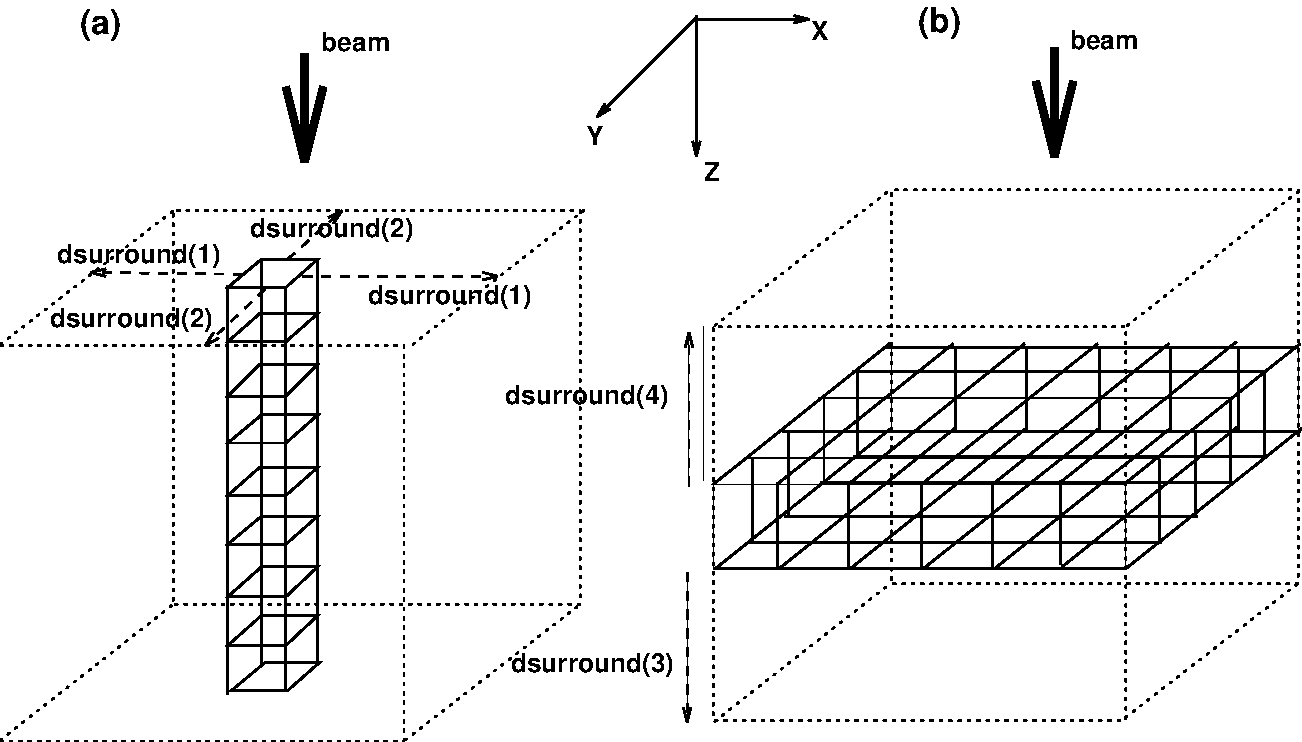
\includegraphics[height=8cm]{figures/dsurround_fig1}
\caption{Two examples of how {\tt dflag} and {\tt dsurround(1...4)} can be used
to
specify a small group of voxels within a larger phantom of the same medium.
In (a) voxels are only specified in a single column for scoring depth-dose,
while the rest of the phantom is defined using {\tt dsurround(1)} and
{\tt dsurround(2)} ({\tt dsurround(3)} and {\tt dsurround(4)} are 0 in this
particular example).  (b) shows voxels specified in a horizontal slice
for scoring the dose profile at a given z value.
In this latter example, the dimensions of the phantom below and above the
slice are defined by {\tt dsurround(3)} and {\tt dsurround(4)} respectively.
{\tt dsurround(1)} and {\tt dsurround(2)} are set to 0 in (b).}
\label{fig_dsurround}
\end{center}
\end{figure}

\lfoot[{{\sffamily \leftmark}}]{{\small Last edited $Date: 2013/09/24 14:49:18 $ }}

Table~\ref{dsurround_table} below shows the results of timing studies
performed using a beam of 10 MeV electrons and a beam
of 6 MV photons incident on a 59x59x10cm water phantom.  For
each beam, 4 cases were simulated: the entire volume filled with 1cm$^{3}$
voxels; 1cm$^{3}$ voxels specified in a column (1x1x10) down
the central (z) axis of the volume (similar to Figure~\ref{fig_dsurround}(a));
1cm$^{3}$ voxels specified in
a vertical slice (1x59x10) through the phantom in the y direction
at x=0; 1cm$^{3}$ voxels specified in a horizontal slice
(59x59x1) through the
phantom at z=2.5cm ($\sim$d$_{max}$)
(similar to Figure~\ref{fig_dsurround}(b)).  In
all cases, simulations were run with and without range rejection.

\begin{table}[htbp]
\caption{Timing results for circular beams of 10 MeV electrons and 6 MV
photons incident on a water phantom.
In all cases, the phantom size is the same (59x59x10 cm$^3$), but the
1x1x1cm$^3$ voxels take up differing parts of the volume (see text).}
\label{dsurround_table}
\begin{tabular}{|p{3cm}|p{3cm}|p{4cm}|p{4cm}|}
\hline
source & number of voxel regions (all 1 cm$^3$) & \multicolumn{2}{|c|}{CPU time (hrs)}\\
\cline{3-4}
       &             & range rejection off & range rejection on \\
\hline
\hline
10 MeV electrons & 59x59x10~~~~~~~ uniform & 0.576 & 0.559 ({\tt ESAVE}=5MeV)\\
\cline{2-4}
(r=10 cm, & 1x1x10 central axis & 0.181 & 0.100 \\
\cline{2-4}
1x10$^{6}$ histories) & 1x59x10 vertical plane & 0.208 & 0.141\\
\cline{2-4}
 & 59x59x1 horizontal plane & 0.345 & 0.300\\
\hline
\hline
6 MV photons & 59x59x10 & 1.623 & 1.525 ({\tt ESAVE}=3MeV)\\
\cline{2-4}
(r=10 cm, & 1x1x10 & 0.785 & 0.479\\
\cline{2-4}
30x10$^{6}$ histories) & 1x59x10 & 0.824 & 0.551\\
\cline{2-4}
 & 59x59x1 & 0.969 & 0.711\\
\hline
\end{tabular}
\end{table}

The table shows that if a depth-dose curve is all that is required, then
specifying voxels only in a 1x1x10cm column can decrease
simulation time by a factor of 5.5 for the electron beam and
a factor of 3 for the photon beam.
In general, the CPU time increases
as the number of voxels specified increases, but orientation of the volume
in which voxels are specified plays a role as well.
The 59x59x1cm horizontal slice
is, relatively, the least efficient use of {\tt dsurround} (saving a factor of
$\sim$2 in CPU time) due to the fact that it has more voxels than the
central-axis phantom and the vertical slice phantom but also due to the fact
that most of the primary and secondary particles from the beam have to be
transported across the
horizontal voxel boundaries defining the slice.  Finally, note that range
rejection is
more efficient when using {\tt dsurround} with a smaller number of
voxels:
turning range rejection on decreases the
simulation time for the case where voxels are only specified in a 1x1x10cm
column by a factor of almost 2, while
its effect on the simulation time when the entire phantom is divided into
voxels is negligible.

Note that this option allows electrons to take much bigger steps in the
{\tt dsurround} regions and this can cause some small inaccuracies unless
the default EGSnrc transport parameters are used.

\section{Pegsless mode}
\indexm{pegsless mode}

As of 2013, DOSXYZnrc can be run independent of the pegs4 cross section data file.  Photon
cross sections had been calculated on the fly since 2006, so the move towards a completely pegsless
version of EGSnrc-based user codes was a logical one.

When running in pegsless mode, all media used in the simulation must be defined
in the {\tt .egsinp} file, between the delimiters, {\tt :start media definition:} and {\tt :stop media definition:}.
{\tt .egsinp} file.  Here, the user has the option of specifying the name of a material data file, containing
\indexm{pegsless mode!material data file}
the compositions, bulk densities, etc, of the media and/or defining media parameters directly in the {\tt .egsinp} file.  The latter method is useful for defining media not included in the material data file or for overriding parameters
in the material data file.  The user also specifies the particle energy limits for cross section calculation:
\indexm{pegsless mode!AE}\indexm{pegsless mode!UE}\indexm{pegsless mode!AP}\indexm{pegsless mode!UP}
{\tt AE} and
{\tt UE} for electrons, {\tt AP} and {\tt UP} for photons.   For more information about the inputs
between the {\tt :start media definition:} and {\tt :stop media definition:} delimiters, including defaults, you are
urged to refer to the BEAMnrc Users Manual\cite{Ro09}.

Pegsless mode is accessible through the DOSXYZnrc GUI by selecting ``Change PEGS4 file'' from the ``File'' menu and
then opting to ``Go PEGSless'' instead of selecting a PEGS4 file.  Once you have done this, a ``Define Media'' button
at the bottom of the main input window becomes active.  Pushing this button will open up a sub-window through
which you have access to the inputs between {\tt :start media definition:} and {\tt :stop media definition:} in
the {\tt .egsinp} file.

\indexm{pegsless mode!running in}
DOSXYZnrc can be run interactively in pegless mode using the command line input:
\begin{verbatim}
dosxyznrc -i inputfile
\end{verbatim}
where {\tt inputfile} is the name of the input file (with no
{\tt .egsinp} extension).

Pegsless batch runs use the command line syntax:
\begin{verbatim}
exb dosxyznrc inputfile pegsless [short|medium|long] [batch=batch_system] [p=N]
\end{verbatim}
This is identical to the syntax of a run with pegs data (see Section~\ref{candrsect} above) but
with the word {\tt pegsless} in place of the name of the pegs data file.

\indexm{pegsless mode!.mederr file}
On termination, pegsless runs output a file, {\tt inputfile.mederr}, containing information about where
the specifications for each medium in the simulation have been read ({\it i.e.} from the material data
file or directly from {\tt inputfile.egsinp}) and various warning messages related to inputs that have
been left blank and have been set to their default values.  The media compositions and settings for other
parameters necessary for calculating cross sections are output to {\tt inputfile.egslst} and
{\tt inputfile.egslog} (for batch runs).

\section{CT Based Phantoms/{\tt ctcreate}}
\indexm{ctcreate}
\indexm{CT!phantoms}

The CT phantom option of DOSXYZnrc allows calculation of dose distributions in
phantoms that are derived from CT data sets. This
allows simulations in realistic anthropomorphic
phantoms. (Please note that the previous sentence does not use the
word patient.)  The creation of CT phantoms from CT data is performed
using the stand-alone code, {\tt ctcreate}.

\indexm{Pinnacle CT}
\indexm{AAPM CT}
\indexm{CT!format!AAPM}
\indexm{CT!format!CADPLAN}
\indexm{CT!format!Pinnacle}
\indexm{CT!format!DICOM}
\indexm{CADPLAN CT}
At this point in time, {\tt ctcreate} supports CT data in DICOM
format (with some restrictions, see below), ADAC
Pinnacle format, and CADPLAN format.
A tool for converting the AAPM CT format into
Pinnacle format is also available.

The process by which CT phantoms are created by {\tt ctcreate}
\indexm{ctcreate}
are outlined here and described in detail in the following sections.

\begin{enumerate}
\item Read in the format of the CT data
\item Read in the CT header parameters (binary or ASCII).
\item Read in the binary CT data.
\item Choose a subset of the CT data set (if desired).
\item Resample the CT data to correspond to volume elements that dose
will be scored in.
\item Convert the CT data to materials and densities for each voxel.
\item Transfer the data via a file to be input to DOSXYZnrc.
\end{enumerate}

\indexm{.egsphant}
\indexm{files!.egsphant}
The relevant CT phantom information
is written into the file, {\tt *.egsphant} (prefix is the same as the
original CT data set name).  A flowchart for the CT phantom code, showing
how it relates to DOSXYZnrc is shown in figure~\ref{fig_ct01}.

Nearly all of the CT phantom functionality takes place outside of
{\tt ctcreate} proper in subroutines.  This
\indexm{ctcreate}
modularity allows for easy changes in the code by ambitious users (for example subroutines for
other CT file formats).  Specifically, this is to provide the user with the
means of reading
their own CT file formats and writing their own dose distribution files
 without rewriting large chunks of
{\tt ctcreate.mortran} and {\tt dosxyznrc.mortran}. This can be accomplished
by creating their
own versions of the subroutines {\tt ReadCT} in {\tt ctcreate.mortran} and
{\tt write\_dose} in {\tt dosxyznrc.mortran}. The
specifications as to what
is required of these subroutines can be found in the codes themselves and
in section~\ref{spec_ReadCT} of this document.

\indexm{CT!coordinate system}
Note that the input CT data set defines the coordinate system for the
calculation, which may be different from the coordinate system of the
accelerator simulation (using BEAM).  For example, for Pinnacle CT
\indexm{Pinnacle CT}
data sets, the Z-axis is typically down the centre of the patient whereas in
the accelerator simulation the Z-axis is the beam's central axis.  This
causes no problems, but must be kept in mind.

\begin{figure}[htbp]
\begin{center}
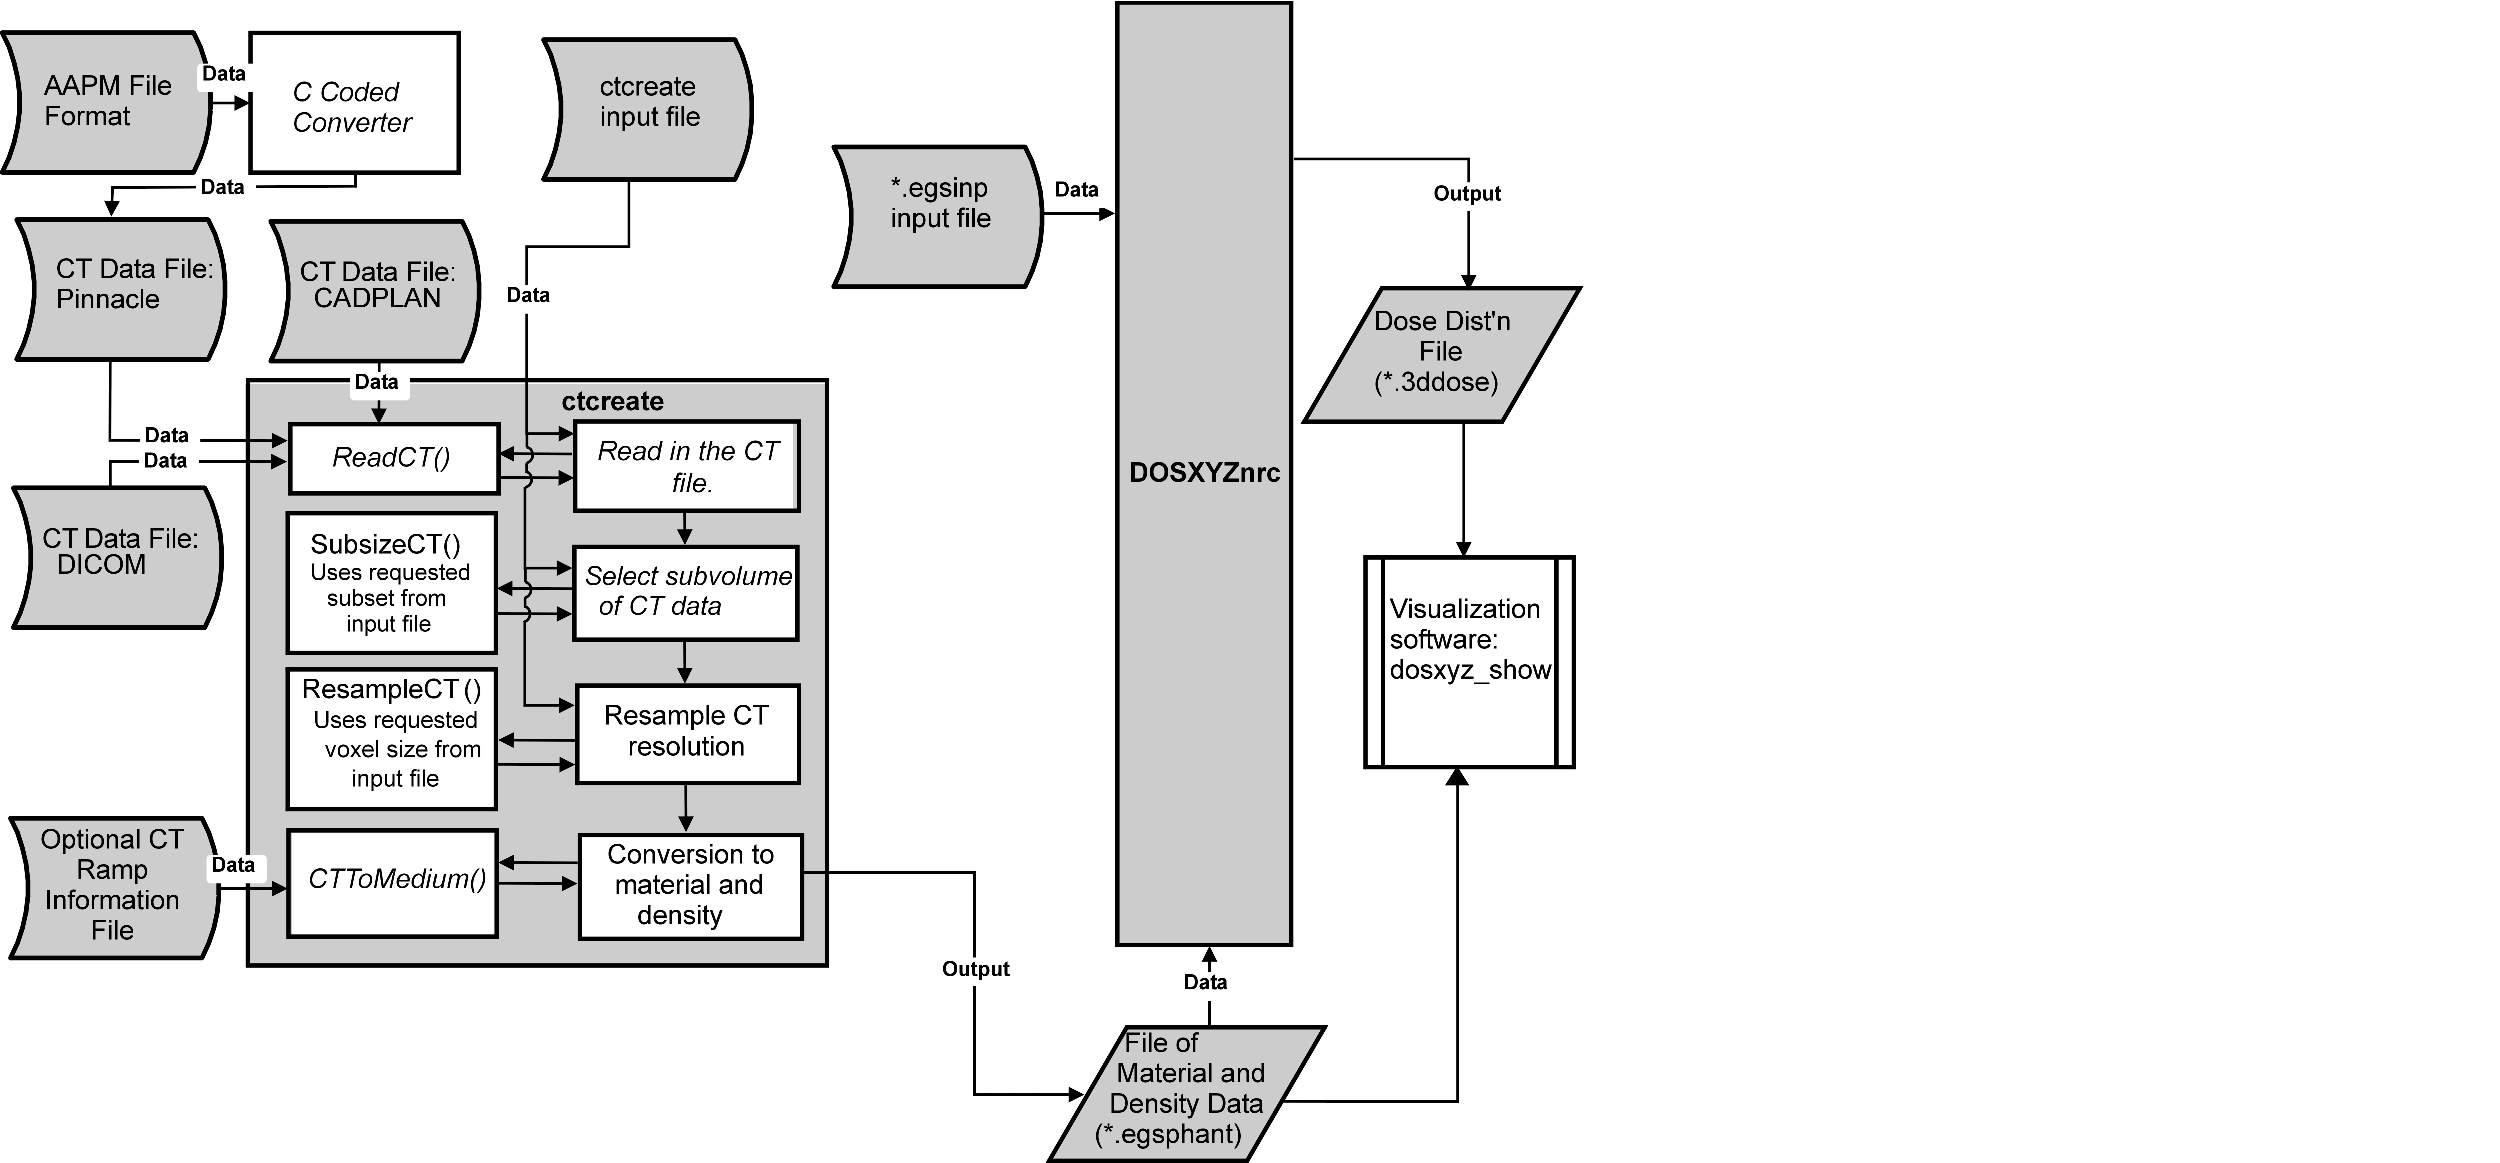
\includegraphics[height=12cm]{figures/ct_fig1}
\caption{A flowchart for use of CT data with  {\tt ctcreate} and DOSXYZnrc. }
\label{fig_ct01}
\end{center}
\end{figure}

\subsection{Using the CT Phantom Option in DOSXYZnrc}

\indexm{CT!option}
\indexm{nmed}
The CT phantom option is used by setting the number of materials,
{\tt nmed} in record 2 of the DOSXYZnrc input file, to zero. This will cause the
program to execute differently than when {\tt nmed} is $>$ 0, and, instead
of geometry, material and density data for the phantom being input explicitly
in the DOSXYZnrc input file,
DOSXYZnrc reads these data from a CT phantom file which has
been created using {\tt ctcreate}.  The input for the
CT and non-CT modes of DOSXYZnrc
are common again after this input (see section~\ref{DOSXYZ_input},
page~\pageref{DOSXYZ_input}).

In short, the input file for DOSXYZnrc is very different if the CT
option is being used.  From section~\ref{DOSXYZ_input} it can be seen
that in CT mode, input records 3-9 in non-CT mode are replaced by
records 3-5, which specify the name of the file containing the CT phantom
data, the transport parameters, and some output parameters.

\subsection{Using {\tt ctcreate}}

\indexm{ctcreate}
\indexm{.egsphant}
\indexm{files!.egsphant}
This section covers the input parameters that {\tt ctcreate} requires
to create a {\tt *.egsphant} CT phantom file that can then be read in and
used by DOSXYZnrc.

It is fairly simple to obtain a
CT phantom from the CT data set since all the required material and geometry
information is contained in the data set.
The additional information that the user is required to provide
are the CT data format, the name of the file containing either the header
info (Pinnacle) or containing the names of the actual CT data files (CADPLAN
and DICOM),
voxel dimensions for the phantom. The user can also select a subset of the full
CT data and specify their own CT ramp (ie function for converting
\indexm{CT!ramp}
CT data to the densities and materials required for the DOSXYZnrc phantom).  Input
of a custom CT ramp is highly recommended.

The following are the input parameters for {\tt ctcreate}.  This description
is found at the beginning of the {\tt ctcreate.mortran} code.
\indexm{ctcreate!input parameters}
\begin{small}
\input{inputs/ctcreate.inp}
\end{small}
\indexm{running ctcreate}

Parameters may be input interactively, by typing:

{\tt ctcreate}

and responding to the prompts;  or stored in an input file
and {\tt ctcreate} run with the input file by typing:

{\tt ctcreate inputfilename}

{\tt ctcreate} input parameters are described in more detail in the subsections below.

\subsubsection{{\tt ctformat}}
\indexm{CT!format}
The first input required by {\tt ctcreate} is the format of the
CT data.  Currently, {\tt ctcreate} supports {\tt Pinnacle}, {\tt
CADPLAN} and {\tt DICOM} formats.
If the data is in AAPM format, then it can be converted to Pinnacle format
using the code
{\tt \$OMEGA\_HOME/progs/ctcreate/CT/AAPM/aapm2pinnacle}
\indexm{aapm2pinnacle}
\indexm{AAPM format}
\indexm{Pinnacle format}
\indexm{CADPLAN format}

\subsubsection{{\tt CTFilename}}
\indexm{CT!data file}
\indexm{CTFilename}
{\tt CTFilename} is the full name of a file, the contents of which depend
on the CT data format:
\begin {description}
\item [Pinnacle format]
\indexm{Pinnacle CT}
{\tt CTFilename} is the full name of the header file of the CT data set
(including the {\tt .header} extension).
The code
will read in all the information that it requires from this file before
moving on to read in the entire binary data file (which has an assumed
extension {\tt .img} and the same prefix as the header file).
  %A sample Pinnacle header file is shown in the next section of this document.
\item [CADPLAN and DICOM formats]
\indexm{CADPLAN CT}
\indexm{DICOM CT}
{\tt CTFilename} is the full name ({\it i.e.} including directory path)
of a file containing the full names of the
individual CT data files (1 file/image slice).  The file names MUST appear
in order of increasing Z position of the slice.
\end{description}

\indexm{.egsphant}
\indexm{files!.egsphant}
On output, the CT phantom will be named:\\
{\tt CTFilename(minus .header extension if using Pinnacle format).egsphant}\\

\subsubsection{{\tt xctsubmin,xctsubmax,yctsubmin,yctsubmax,zctsubmin,zctsubmax}}
\indexm{CT!sub-volume}
\indexm{xctsubmin}
{\tt xctsubmin},{\tt xctsubmax}, {\tt yctsubmin}, {\tt yctsubmax},
{\tt zctsubmin},
and {\tt zctsubmax} are used to create six planes which describe a cube.
The subsection of the original CT data contained in this cube will
be used to create the CT phantom. In this
manner only the portion of interest in the original CT data is used in
the simulation.  This allows the particle simulation
to be performed at a higher resolution than if the calculation used the
entire CT volume, and allows the user to trim some of the air that surrounds
a typical CT image from consideration in the phantom.  Note that if the
sub-volume selected by the user does not fit on an integer number of voxels
from the original CT data, then the sub-volume will automatically be expanded
until it does so.

\subsubsection{{\tt xyz\_xthickness,xyz\_ythickness,xyz\_zthickness}}
\indexm{CT!phantom voxels}
\indexm{voxel size}
\indexm{xyz\_xthickness}
The third line of the input to {\tt ctcreate} is the
spatial resolution that the user requires for the simulation.
{\tt xyz\_xthickness}, {\tt xyz\_ythickness}, {\tt xyz\_zthickness}
are the 3 dimensions of the voxels to be used in the CT phantom.
The maximum voxel dimension in a given direction is
the distance between the planes delimiting the subset of the CT data
to be used in that direction (see previous section).
The minimum voxel dimension in a direction is the distance between
the planes delimiting the subset of CT data in that direction divided
by the maximum number of voxels allowed in that direction (set at
compilation).
{\tt ctcreate} will alert the user when dimensions less than the minimum
or greater than the maximum are input.  Note that, if necessary, the voxel
dimensions will always be increased to fit an integer number of DOSXYZnrc
voxels on the CT sub-volume selected by the user.

\subsubsection{{\tt num\_material}, {\tt material\_ct\_lower\_bound}, and other CT ramp inputs}
\indexm{CT!ramp}

{\tt num\_material} is the
number of materials in the ramp function used
to convert CT number in each voxel to material and density.
If this is set to zero then a
default CT ramp is used in the conversion. The default ramp
is shown in Figure~\ref{fig_ct02} and in the sample input file given in the next section.
{\tt material\_ct\_lower\_bound} defines the lowest CT number of the first ramp
({\it i.e.} the lowest CT number for material  1).  If the default ramp is used, then {\tt material\_ct\_lower\_bound} defaults
to -1024, which is typically the minimum CT number for air in DICOM format data.

If {\tt num\_material} $>$0 then
the CT ramp is read from
the input file.  For each medium in the ramp, there are
two lines of input. \indexm{CT!ramp}
The first of these lines is the name of the material
({\tt material\_name}) which must be identical to a material in the
{\tt PEGS4} material data file being used in the DOSXYZnrc simulation.
The second line specifies the maximum CT number for the medium, {\tt material\_ct\_upper\_bound},
the minimum density of the medium, {\tt material\_density\_lower\_bound}, and the maximum
density of the medium,
{\tt material\_density\_upper\_bound}. Note that the ramp is assumed to be continuous
in CT number.  Thus, for material {\tt n}, {\tt material\_density\_lower\_bound(n)} corresponds
to a CT number of {\tt material\_ct\_upper\_bound(n-1)} (or the overall
minimum CT no. of the ramp, {\tt material\_ct\_lower\_bound}, if
{\tt n}=1), and {\tt material\_density\_upper\_bound(n)} corresponds to
{\tt material\_ct\_upper\_bound(n)}.
Also note that the ramp must be input in order of
increasing {\tt material\_ct\_upper\_bound}.

The CT ramp is then used to determine the medium and density in each voxel of the CT data.
\indexm{CT!ramp}
If a voxel's CT number is $\leq$ {\tt material\_ct\_upper\_bound(n)} and
$>$ \\
{\tt material\_ct\_upper\_bound(n-1)} (or {\tt material\_ct\_lower\_bound} if
{\tt n}=1)
then it is assigned medium {\tt n}. The density is then calculated using a linear
interpolation between the medium's density limits:
\begin{align}
{\tt r}&{\tt hor}_{i,j,k} = {\tt material\_density\_lower\_bound(n)} \nonumber \\
             &+\left(\frac{{\tt material\_density\_upper\_bound(n)}-
 {\tt material\_density\_lower\_bound(n)}}
{{\tt material\_ct\_upper\_bound(n)}-
 {\tt material\_ct\_upper\_bound(n-1)}}\right)        \\
        &*({\tt CT}_{i,j,k}-{\tt material\_ct\_upper\_bound(n-1)}) \nonumber
\end{align}

The default ramp is shown in Figure~\ref{fig_ct02}. This is a modified version of
\indexm{CT!ramp}
a CT ramp given in Kawrakow et al\cite{Ka96a}.  Note that this ramp has been
optimized for typical DICOM format data, where the lowest CT number for air
{\tt material\_ct\_lower\_bound} is -1024.

If the CT number in a voxel is less than {\tt material\_ct\_lower\_bound} then
the medium in that voxel is set to vacuum with density zero.
Those voxels with CT numbers above the
last material's upper CT number ({\tt material\_ct\_upper\_bound(num\_material)})
will have the density set to the maximum
density for the last material.

\begin{figure}[H]
\begin{center}
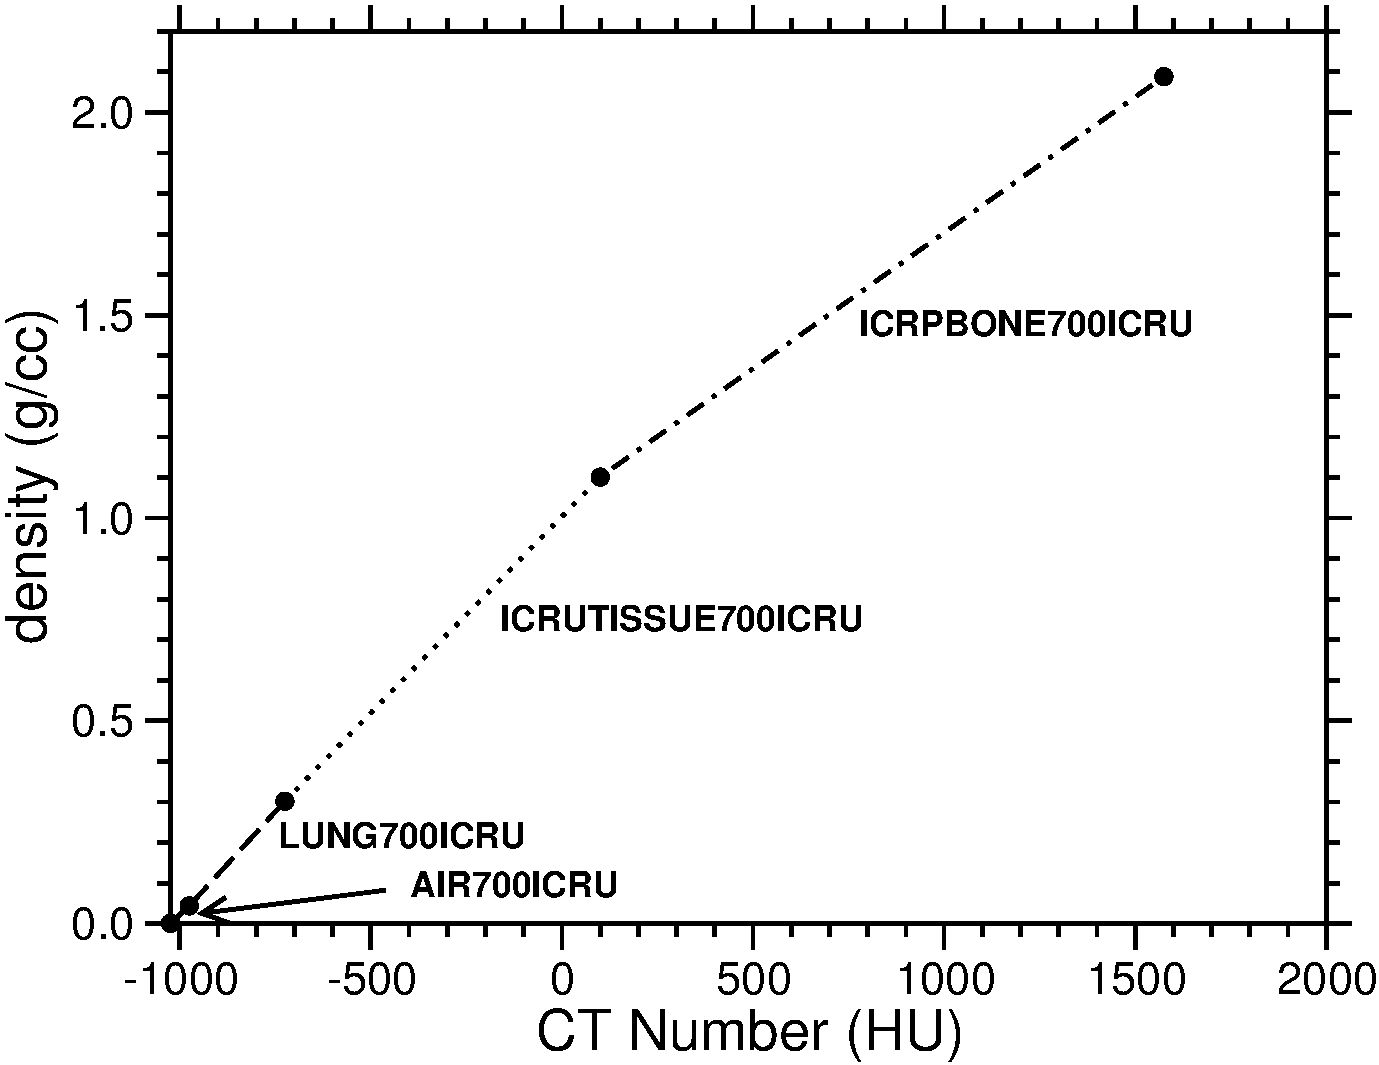
\includegraphics[width=10.5cm]{figures/CTramp}
\caption{The default ramp for converting CT values to material and
density in {\tt ctcreate} modified from Kawrakow et al\cite{Ka96a}.}
\label{fig_ct02}
\end{center}
\end{figure}
\indexm{CT!ramp}

The default CT ramp may be suitable for displaying a {\tt .egsphant} file
using {\tt dosxyz\_show}\cite{Ka98} and for example calculations.  However,
we strongly recommend that you explicitly enter your own CT ramp function
for more detailed simulations, since the CT ramp is
dependent upon the imager and the data acquisition method.

\subsection{Sample {\tt ctcreate} CT Phantom Input File}
\indexm{ctcreate!sample input}
Table~\ref{ctinpex} shows an example {\tt ctcreate} input file, and
a sample DOSXYZnrc input file (excluding EGSnrc inputs)
which uses the CT phantom data from {\tt ctcreate}.

\vspace*{-0.5cm}
\begin{table}[htbp]
%\begin{tabular}{|p{8cm}p{7.7cm}|}
\caption{Sample input files for {\tt ctcreate} and DOSXYZnrc}
\begin{tabular}{|p{7cm}p{8.7cm}|}
\hline
\bf{Input Parameter} & \bf{Description of input fields.} \\
\multicolumn{2}{|c|}{\bf for {\tt ctcreate}      } \\
{\tt DICOM} & CT data is in DICOM format \\
{\tt CTfname} & in DICOM format, this is the name of a file containing the names of the individual image slices (in order
of increasing Z).
\\
%\hline
{\tt -17.64,17.64,-17.64,17.64,-0.7,4.3}
&
The subvolume of the CT data set
that is to be used for the phantom.
\\
%\hline
{\tt 1.0, 1.0, 1.0 }
&
The phantom voxel size.
\\
%\hline
{\tt 4, -1024}
&
{\tt num\_material}, {\tt material\_ct\_lower\_bound}.
If {\tt num\_material}=0
the default ramp will be used.
The default values are
listed explicitly in this example.
\\
%\hline
{\tt AIR700ICRU }
&
The material\_name for the first material.
\\
%\hline
{\tt -974,0.001,0.044}
&
CT ramp parameters for the first material:\\
&{\tt  material\_ct\_upper\_bound}, \\
&{\tt material\_density\_lower\_bound},\\
&{\tt material\_density\_upper\_bound}
\\
%\hline
{\tt LUNG700ICRU }
&
The material name for the second material.
\\
%\hline
{\tt -724,0.044,0.302}
&
The ramp parameters for the second material. \\
%\hline
{\tt ICRUTISSUE700ICRU} & The material name for the third material.
\\
%\hline
{\tt 101,0.302,1.101} & The ramp parameters for the third material.
\\
%\hline
{\tt ICRPBONE700ICRU} & The material name for the fourth material.
\\
%\hline
{\tt 1976,1.101,2.088} & The ramp parameters for the fourth material.
\\
\hline
\multicolumn{2}{|c|}{\bf for DOSXYZnrc} \\
%\hline
{\tt Sample CT Input File } & Title of the simulation and phantom. \\
%\hline
0 & {\tt NMED } - If this is zero the code switches to CT\_Phantom mode. \\
%\hline
{\tt CTfname.egsphant} & The name of the CT phantom file.\\
{\tt 0.7,0.01,5.0} & {\tt ECUTIN}, {\tt PCUTIN}, {\tt SMAX} (dummy inputs)\\
{\tt 1,0,1} & {\tt zeroairdose}, {\tt doseprint} and {\tt MAX20} \\
%\hline
{\tt -1,0,-1.25,1.25,-2.25,2.25,90.0,} & The source description record.
At this point the \\
{\tt 90.0,0.0} &CT phantom input meets up with the manual\\
& phantom inputs.
\\
%\hline
{\tt 0}
&
monoenergetic particle spectrum.
\\
%\hline
{\tt 20.0 }
&
particle energy.
\\
%\hline
{\tt 100,0,500.,7,3,100.,0,0,0,1,5.0,} & Monte Carlo information (note range rejection \\
\hspace*{1cm}{\tt 0,0,0,0}&below 5MeV).  \\
%\hline
\hline
\end{tabular}
\label{ctinpex}
\end{table}

\subsection{Location of {\tt ctcreate} and How to Compile It}
\label{comp_ctcreate}
{\tt ctcreate.mortran} and related files
(see section~\ref{filesect} for a complete list)
\indexm{ctcreate!installation}
reside in the subdirectory {\tt \$OMEGA\_HOME/progs/ctcreate}.
Normally, it is compiled as part of the OMEGA/BEAM installation
(see the BEAMnrc Manual\cite{Ro04a} for installation instructions), however
it can be compiled separately by going into this directory and
typing {\tt make}.

\subsection{{\tt ReadCT()} Subroutines}
\label{spec_ReadCT}
\indexm{ReadCT}
\indexm{CT!format!AAPM}
\indexm{CT!format!CADPLAN}
\indexm{CT!format!DICOM}
\indexm{CT!format!Pinnacle}
{\tt ReadCT} is the most important subroutine in {\tt ctcreate}.  It handles
the reading in of header information and binary CT data.  Currently, there
are three {\tt ReadCT} subroutines within {\tt ctcreate}, one for each of the CT formats
supported: {\tt ReadCT\_Pinnacle} for Pinnacle, {\tt ReadCT\_CADPLAN}
for CADPLAN data and {\tt ReadCT\_DICOM} for DICOM data.

\subsubsection{{\tt ReadCT\_Pinnacle}}
\indexm{ReadCT\_Pinnacle}
\indexm{CT!format!Pinnacle}

{\tt ReadCT\_Pinnacle} is contained
within the {\tt ctcreate.mortran} file and calls
other subroutines and functions in this file:
\begin{description}
\indexm{ReadReal}
\indexm{ReadInt}
\indexm{read\_ct\_data}
\indexm{swap\_bytes}
\item[{\tt ReadReal}] Reads real values from the image header ({\tt .header}) file.
\item[{\tt ReadInt}] Reads integer values from the header file.
\item[{\tt read\_ct\_data}] Reads binary CT data from the image ({\tt .img})
file.
\indexm{swapping bytes}
\item[{\tt swap\_bytes}] Swaps bytes of CT data if there is a
byte order mismatch between the data and the machine you are using.
\end{description}

Note that in Pinnacle format CT numbers are $>$ 0.  Thus, the default CT ramp
in {\tt ctcreate} cannot be used to convert CT numbers to media and densities.
The example {\tt ctcreate} inputfile, {\tt \$OMEGA\_HOME/progs/ctcreate/ctcreate\_examples/CT\_create.inp}
(used in Lab VI in the BEAMnrc Workshop), is used to convert Pinnacle format data and
contains a custom CT ramp which is just the default ramp shifted up by 1025 HU.

\subsubsection{{\tt ReadCT\_CADPLAN}}
\indexm{ReadCT\_CADPLAN}
\indexm{CT!format!CADPLAN}
{\tt ReadCT\_CADPLAN} is also contained
within the {\tt ctcreate.mortran} file.
Unlike {\tt ReadCT\_Pinnacle}, {\tt ReadCT\_CADPLAN} is a self-contained subroutine.
Byte swapping is not required since single bytes are read at a time.


\subsubsection{{\tt ReadCT\_DICOM.c}}
\indexm{CT!format!DICOM}
\indexm{ReadCT\_DICOM}
{\tt ReadCT\_DICOM.c} is a separate C routine whose object file is linked
to {\tt ctcreate} at compile time.  {\tt ReadCT\_DICOM.c} is automatically
compiled when you {\tt make} ctcreate.
{\tt ReadCT\_DICOM.c} requires the C header file {\tt tags\_ct.h}, which
defines hexadecimal tags, or labels, for the DICOM data.  These tags
are defined in the DICOM standard, and if the user modifies
{\tt ReadCT\_DICOM.c} to deal with additional tags, then these can
be added to the {\tt tags\_ct.h} file.
Currently,
{\tt ReadCT\_DICOM} assumes
\indexm{little endian byte order}
\indexm{big endian byte order}
the DICOM data has been collected on a machine with little endian byte order
(ie compatible with Linux), however, if the data was collected on a machine
with big endian byte order, you must go into {\tt ReadCT\_DICOM.c} and
change the line:
\indexm{DICOM\_ENDIAN}
\begin{verbatim}
#define DICOM_ENDIAN 1
\end{verbatim}
to:
\begin{verbatim}
#define DICOM_ENDIAN 0
\end{verbatim}
and recompile {\tt ctcreate}.  The endianness of the machine you
are running {\tt ctcreate} on is automatically detected by
{\tt ReadCT\_DICOM} and then bytes are swapped if necessary.

The DICOM format is known to vary from imager to imager and institute
to institute.  Thus, we cannot guarantee that {\tt ReadCT\_DICOM} will
work with your images without modification.  As a minimum,
the current version of {\tt ReadCT\_DICOM} requires the following
information in the image (slice) header(s):
\begin{enumerate}
\item Number of rows (data tag {\tt 0x00280010}).  This defines the number of voxels in the X-direction.
\item Number of columns (data tag {\tt 0x00280011}). This defines the number of voxels in the Y-direction.
\item Pixel spacing (data tag {\tt 0x00280030}).  Defines the X- and Y-dimensions of the voxels.
\item Image position (data tag {\tt 0x00200032}). Defines the (X,Y,Z) of the centre of the first voxel.  The position
of the first slice (slice with lowest Z) is used to determine the X-, Y- and
Z-offset (starting position) of the CT data, and the Z-positions of the first two slices are used
to established voxel Z-dimension ({\it i.e.} slice thickness).
The Z-positions of slices as read from the header are also used to
sort slices in order of increasing Z, in case the user has not already done so
in the file containing the slice names.
\item A pixel data tag ({\tt 0x7fe00010}) indicating the size of the data array in bytes.  This tag must appear last in the
header, immediately preceding the CT data itself.
\end{enumerate}

{\tt ReadCT\_DICOM} assumes slices are contiguous in Z.  Thus, once the Z-position of the first slice and slice thickness (Z-dimension of voxels) are
established, {\tt ReadCT\_DICOM} positions subsequent slices so that there are no gaps
or overlaps between them.  A warning message is output if the Z-position of
a slice determined by {\tt ReadCT\_DICOM} does not equal the Z-position
of the slice as read from the image position in its header.

We note that {\tt ReadCT\_DICOM.c} has limited flexibility in terms of slice
layout, and it has not been
tested on all possible variations of the DICOM format.  Therefore, if you
require more flexibility or are having trouble converting your DICOM files, you
are strongly urged to either modify {\tt ReadCT\_DICOM} or use your own
stand-alone routine for converting DICOM images to {\tt .egsphant} files.

\indexm{Nick Reynaert}
The initial version of {\tt ReadCT\_DICOM.c} was provided by Nick Reynaert at the University of Ghent.

\subsubsection{Generic {\tt ReadCT}}
\indexm{ReadCT!Generic}

Essentially, {\tt ReadCT} is the subroutine or stand-alone
code which the user will have to
\indexm{ReadCT specs}
customize or program from scratch to deal with any CT format not currently
handled.  The structure and number of subroutines within {\tt ReadCT} is
largely a matter of the programmer's taste.  However, if {\tt ReadCT} is
to be included in {\tt ctcreate} (or linked as an object file when compiling
{\tt ctcreate}), it must
pass certain essential data back to {\tt ctcreate}.   An example call to
a generic {\tt ReadCT} routine is:

\noindent {\tt Subroutine ReadCT(fname,asize,ctdata,offset,vsize,error)}

\noindent where {\tt fname} is a character string containing the name of the
particular CT data set.  The essential CT data returned to {\tt
ctcreate} are:
\begin {description}
\item [{\tt asize(3)}]  An array returning the number of CT voxels in the
                     x,y,z directions.
\item [{\tt vsize(3)}]  An array returning the dimensions of the CT voxels

\item [{\tt offset(3)}] An array returning the lower bounds of the CT data
                      in the x,y,z directions in cm.
\item [{\tt ctdata(\$CTIMAX,\$CTJMAX,\$CTKMAX)}] A 3-D integer array
           returning the CT data (Hounsfield numbers).  In {\tt ctdata},
    {\tt x}$\rightarrow${\tt i},
    {\tt y}$\rightarrow${\tt j},
    {\tt z}$\rightarrow$ {\tt k}, so that {\tt ctdata(i,j,k)} is
    equal to the Hounsfield number in the voxel with lower bounds
    {\tt x=offset(1)+(i-1)*vsize(1)}, {\tt y=offset(2) +} {\tt (j-1)*vsize(2)},
    {\tt z=offset(3)+} {\tt (k-1)*vsize(3)} and
    upper bounds {\tt x=offset(1)+} {\tt i*vsize(1)},
    {\tt y=offset(2)+} {\tt j*vsize(2)}, {\tt z=offset(3)+} {\tt k*vsize(3)}
\item [{\tt error}] Returns the error status of the CT read operation.
                    Currently not used.
\end {description}

\subsection{Description of the {\tt *.egsphant} File}
\label{egsphantsect}
\indexm{.egsphant}
\indexm{files!*.egsphant}
The {\tt *.egsphant} file output by {\tt ctcreate} or by DOSXYZnrc itself
is an ASCII file
containing the following information necessary for DOSXYZnrc to simulate
the CT phantom and for the display program, {\tt dosxyz\_show}\cite{Ka98},
to display the density information:
\begin{enumerate}
\item The number of media in the phantom
\item The names of the media
\item The {\tt ESTEPE} value for each medium (now a dummy input)
\item The number of voxels in the X, Y and Z directions
\item A list of the voxel boundaries in the X direction
\item A list of the voxel boundaries in the Y direction
\item A list of the voxel boundaries in the Z direction
\item For each Z slice, an X-Y array containing the medium
      number in each voxel
\item For each slice in the Z direction, an X-Y array containing the densities
      in each voxel
\end{enumerate}
\vspace*{-0.3cm}
In addition to passing the necessary medium information to DOSXYZnrc, the X-Y
arrays of medium numbers (item 8 above) provide a rough slice-by-slice
view of the CT phantom.  A sample X-Y array of medium numbers from one slice of a CT phantom derived
from a lung image is shown below (hold at a distance, and raw data on
screen is easier to see):

\input{inputs/mednoarray.inp}

The user can use these slice-by-slice views to
determine whether the CT data is being read in correctly by {\tt ReadCT}
or to verify that the sub-volume of the original CT data selected
includes the physiology of interest.

\subsection{Files and Macros for implementation.}
Below is a short description of the files and macros required to compile
and run {\tt ctcreate} and DOSXYZnrc with CT phantoms.
\indexm{ctcreate!files and macros}

\begin{description}
\item[{\tt dosxyznrc\_user\_macros.mortran}]
{\tt ctcreate} uses the version stored in\\
{\tt \$HEN\_HOUSE/user\_codes/dosxyznrc}
to obtain {\$IMAX}, {\$JMAX} and {\$KMAX},
the maximum X, Y and Z dimensions of the CT phantom allowed in DOSXYZnrc.

\item[{\tt \$CTIMAX, \$CTJMAX, \$CTKMAX }]
Macros defining the maximum X, Y and Z dimensions of the CT data to be read in.
These macros are in {\tt ctcreate.mortran}

\item[{\tt lnblnk1.mortran}] {\tt MORTRAN} macro to provide the
FORTRAN {\tt lnblnk} function for Linux, rs6000 and HP9000 machines.
{\tt ctcreate} makes extensive use of this function and DOSXYZnrc uses it
in CT phantom mode.  It
is read from the {\tt \$HEN\_HOUSE/src} directory
\end{description}

\section{Known Bugs/Restrictions}

A resumed run that uses a phase space source with particle recycling will
not produce dose/uncertainty results identical to a single run with
the same total number of histories.  This is because the last particle
used before resuming may not have been recycled the full
{\tt NRCYCL} times, and resuming automatically skips to the next particle.
Results will agree within uncertainty, however.

It is recommended that when using the built-in parallel processing
functionality you do not resume parallel runs that use
a phase space source.  In this case, parallel jobs have lost track
of which chunks of the phase space source they were using in the
original run and the uncertainty analysis after recombining the
resumed runs will not take into account correlations due to reusing
chunks of the phase space source.

\section{Acknowledgments}

Charlie Ma was a major contributor to the DOSXYZ code and was the senior
author of the original DOSXYZ manual. Since he is not directly involved
with DOSXYZnrc, he is no longer an author of the manual, but his
contribution to the original code while he was at NRC still plays a
significant role in the current version.


A variety of people have contributed various pieces of code to the
DOSXYZnrc program.  We wish to thank: Julie Zachman of UW for providing
the aapm2pinnacle tool; Daryoush Sheikh-Bagheri for developing PAW
macros for displaying dose distributions and CT files; Geoff Zhang and
Daryoush again for extensive use of the code and drawing our attention
to bugs; Alex Bielajew for early work on the code; Marc Lauterbach and
Joerg Lehmann for initial coding to read CADPLAN CT data sets.
We also wish to thank Paul Reckwerdt for his work on the original code to
read Pinnacle CT data sets; Mark Holmes for his extensive work on reading
CT data and for coding the correlated sampling routines\cite{Ho99}; Brian
Geiser for the BTREE beam modeling method\cite{Ge95}.  \indexm{CADPLAN CT}

\begin{latexonly}
\section{References}
\end{latexonly}
\renewcommand{\rightmark}{References}
\indexm{references}
\typeout{****references start here}
\setlength{\baselineskip}{0.4cm}
\vspace*{-1cm}
\bibliography{../irs}
\bibliographystyle{unsrt}


\newpage
\setlength{\baselineskip}{0.5cm}
\input{pirs794-dosxyznrc.ind}

\end{document}


\end{document}


\end{document}


\end{document}
